\chapter{Lo básico para redacción}
\label{cha:lo_basico}


Asumiré que leíste el capítulo \ref{cha:introduccion} y sabes utilizar el botón \emph{Recompilar} en Overleaf, o que sabes cómo compilar un documento por tus propios medios (si no es así, ahora es un buen momento para regresar a la sección \ref{sec:un_primer_documento}).

De aquí en delante, no habrá muchas imágenes ni explicaciones paso a paso, simplemente las instrucciones utilizadas y su resultado, dentro del mismo documento.



\section{El idioma español}
\label{sec:el_idioma_espanol}



Aunque ya tenemos el paquete \texttt{inputenc} para introducir caracteres del idioma español, los textos de las figuras aparecen como \emph{Figure}, y el del índice como \emph{Contents}. Además, \LaTeX{} está usando las reglas de segmentación de palabras del idioma inglés (puedes buscar el tema como \emph{hyphenation}).

Para traducir estos diversos textos, y separar bien las palabras, hay que utilizar otro paquete\footnote{Espero que ya vayas captando que así se resuelve la vida en \LaTeX{}}: \texttt{babel}, y debe ser configurado con la opción \texttt{spanish}. Como, por alguna extraña razón, traduce ``Table'' como ``Cuadro'', es necesario agregar alguna de estas opciones:
\begin{itemize}
	\item \texttt{es-tabla}, la cual sirve para traducir ``Cuadro'' como ``Tabla'', como debería ser.
	\item \texttt{mexico}, que incluye el ajuste de \texttt{es-tabla}, entre otros más.
\end{itemize}

Para este libro, yo utilicé la opción \texttt{mexico}. En caso de querer colocar dos valores dentro de un comando de \LaTeX{} es necesario separarlos por coma, por lo que los dos valores a ser pasados al paquete \texttt{babel} se enlistan como \texttt{spanish,mexico}:

\begin{lstlisting}[style=latex,numbers=none]
\usepackage[spanish,mexico]{babel} % Idioma español, texto "Tabla".
\end{lstlisting}

Si quieres saber más respecto a la opción \texttt{mexico}, consulta \cite{bib:opciones_spanish}.



\section{Formato}
\label{sec:formato}



A lo largo del capítulo anterior ya utilizamos \emph{texto en cursiva}, \textbf{texto en negritas}, y \texttt{texto en fuente de ancho fijo}, sin informar qué instrucciones fueron necesarias. La tabla \ref{tab:instrucciones_estilo} muestra las instrucciones correspondientes, con un ejemplo... más el subrayado, que esperemos no tengas que utilizar en exceso. Según se aprecia en el ejemplo, el estilo se aplica al contenido que existe entre llaves (\{ y \}).

\begin{table}[ht!]
\centering
\begin{tabular}{lll}
\hline
\multicolumn{1}{c}{\textbf{Si queremos...}} & \multicolumn{1}{c}{\textbf{Usamos...}} & \multicolumn{1}{c}{\textbf{Y resulta...}}   \\
\hline
Texto en cursiva    & |\emph{¡Qué estilo!}|         & \emph{¡Qué estilo!}             \\
Texto en negritas   & |\textbf{Hola :D}|            & \textbf{Hola :D}                \\
Texto de ancho fijo & |\texttt{suma = 42 + 16;}|    & \texttt{suma = 42 + 16;}        \\
Texto subrayado     & |\underline{subrayado...}|    & \underline{subrayado...}        \\
\hline
\end{tabular}
\caption{Cursivas, negritas, subrayado, y ancho fijo en \LaTeX.} % Leyenda de la tabla.
\label{tab:instrucciones_estilo}
\end{table}



\subsection{Una nota sobre \ttlatex{emph} y \ttlatex{textit}}
\label{sub:una_nota_sobre_emph_y_textit}



Hay otra intrucción en \LaTeX{} que puede hacer letras cursivas\footnote{Varias, de hecho...}. Quizá te topes con la instrucción |\textit|, pues también imprime cursivas en pantalla. No obstante, se prefiere el uso de |\emph| debido a que se puede anidar con negritas, además de otras consideraciones que no son de mucho interés \cite{bib:emph}.

En resumen, puedes utilizar |\textit| para cursivas, pero se recomienda más |\emph| (recomendación hecha también por Overleaf \cite{bib:overleaf_emph}).



\section{Espacio en blanco en \LaTeX}
\label{sec:espacio_en_blanco_en_latex}



Hemos de recordar que \LaTeX{} no es un editor \emph{WYSIWYG}. ¿Y eso qué? Que, en Word, si das un \texttt{Enter}, tienes una nueva línea. Si das dos \texttt{Enter}, tienes dos nuevas líneas. Y si das cincuenta \texttt{Enter}, posiblemente llegues a una nueva página.

En \LaTeX{}, un \texttt{Enter} es un simple espacio. Dos \texttt{Enter} son un cambio de párrafo. Cincuenta \texttt{Enter} siguen siendo un cambio de párrafo. ¿Por qué? Porque \LaTeX{} se basa en instrucciones para posicionar el texto, no en el espacio en blanco. Tanto así que el compilador colapsa el espacio en blanco al momento de traducir tus instrucciones a PDF. Eso implica que los saltos de línea, los espacios, las tabulaciones... todo se colapsa a uno solo. Lo que es más, tú nunca llegas a tener una idea visual de dónde se producirá un cambio de página hasta que ves el PDF producido. De momento, para ver los efectos del espacio en \LaTeX{} tenemos el fragmento del listado \ref{lst:fragmento_espacios}, con el símbolo \lstinline[showspaces=true,columns=fixed]! ! para señalar donde hay espacios en blanco.

\begin{lstlisting}[style=latex,numbers=left,showspaces=true,label=lst:fragmento_espacios,caption={Fragmento de texto para demostración de espacio en blanco.}]
[Hola,            aquí         hay         mucho,          	
pero mucho]       			
        	
           		
[           espacio                    ]
       	
            	
                    	
[				¿No crees?]   	
\end{lstlisting}

A pesar de que el fragmento cuenta con nueve líneas, en el PDF se traducen a:

\begin{displayquote}{}
[Hola,            aquí         hay         mucho,          	
pero mucho]       			
        	
           		
[           espacio                    ]
       	
            	
                    	
[				¿No crees?]   	
\end{displayquote}

¿Qué pasó? Como dijimos anteriormente, \LaTeX{} cuenta un salto de línea como un espacio, razón por la cual las primeras dos líneas del fragmento en el listado \ref{lst:fragmento_espacios} se colapsaron a una sola. Donde había dos o más saltos de línea se produjo un cambio de párrafo. Sobre los demás espacios... bueno, se colapsaron a uno solo. Es decir, no importa si separas una palabra con uno o veinte espacios, \LaTeX{} los colapsará a uno solo. Lo bueno de esto es que ya no tendrás que preguntarte si el espacio entre dos palabras es de uno o dos espacios, o preguntarte por qué se subraya algo con color azul (te estoy viendo a ti, Word).

Fuera de juego, \LaTeX{} nos trae un beneficio: puedes usar todo el espacio en blanco que quieras para acomodar tu documento al estar editando. Claro, todo don trae una maldición: ¿ahora cómo se supone que uno inserte espacios de más?

La respuesta viene de la mano de instrucciones y caracteres especiales, obvio. Así es esto en \LaTeX{}, y espero que ya te estés acostumbrando a ese hecho. Si quieres espacios en blanco, usas el carácter \textbf{\textasciitilde} (sí, la virguilla o tilde de la eñe). Para tener muchos espacios, cambiamos el texto a:

\begin{lstlisting}[style=latex,numbers=none]
[Hola,~~~~~~~~~~~~aquí~~~~~~~~~hay~~~~~~~~~mucho~~~~~~~~~~~
pero mucho]~~~~~~~~~~~~~~~~~
\end{lstlisting}

\noindent Lo que ya nos da el resultado esperado en los espacios entre palabras:

\begin{displayquote}{}
[Hola,~~~~~~~~~~~~aquí~~~~~~~~~hay~~~~~~~~~mucho~~~~~~~~~~~
pero mucho]~~~~~~~~~~~~~~~~~
\end{displayquote}

¿Y qué hay de las tabulaciones? Siempre son un problema. ¿A cuántos espacios equivale una tabulación? ¿Qué comando se utiliza? Aunque hay varios, como |\quad|, recomiendo simplemente usar cuatro tildes consecutivas (|~~~~|) cada vez.

¿Y para insertar líneas adicionales? Se puede utilizar la instrucción |\newline| según la cantidad de líneas que queramos colocar, como se muestra en el listado \ref{lst:espacio}.

\begin{lstlisting}[style=latex,label=lst:espacio,caption={Espacio en blanco en \LaTeX{}.}]
[Hola,~~~~~~~~~~~~aquí~~~~~~~~~hay~~~~~~~~~mucho~~~~~~~~~~~
pero mucho]~~~~~~~~~~~~~~~~~
\newline\newline
[~~~~~~~~~~~espacio~~~~~~~~~~~~~~~~~~~~]
\newline
\newline
[~~~~~~~~~~~~~~~~¿No crees?]
\end{lstlisting}

Ya sea que pongamos ambas instrucciones |\newline| en la misma línea, o cada una en su propia línea, el resultado es el mismo, se muestran dos saltos de línea:

\begin{displayquote}{}
[Hola,~~~~~~~~~~~~aquí~~~~~~~~~hay~~~~~~~~~mucho~~~~~~~~~~~
pero mucho]~~~~~~~~~~~~~~~~~
\newline\newline
[~~~~~~~~~~~espacio~~~~~~~~~~~~~~~~~~~~]
\newline
\newline
[~~~~~~~~~~~~~~~~¿No crees?]
\end{displayquote}

Empero, |\newline| no es el único comando utilizado para realizar saltos de línea, puede que llegues a ver su ``gemelo'' malvado, la instrucción \codigo{\textbackslash}. ¿Por qué malvado? En algunas ocasiones puede ocurrir algún error como el siguiente:

\begin{lstlisting}[style=errores]
Missing number, treated as zero. [[~~~~~~~~~~~espacio~~~~~~~~~~~~~~~~~~~~]]
Illegal unit of measure (pt inserted). [[~~~~~~~~~~~espacio~~~~~~~~~~~~~~~~~~~~]]
Argument of \language@active@arg~ has an extra }. [[~~~~~~~~~~~espacio~~~~~~~~~~~~~~~~~~~~]]
Paragraph ended before \language@active@arg~ was complete. [[~~~~~~~~~~~espacio~~~~~~~~~~~~~~~~~~~~]]
Missing number, treated as zero. [[~~~~~~~~~~~~~~~~¿No crees?]]
Illegal unit of measure (pt inserted). [[~~~~~~~~~~~~~~~~¿No crees?]]
\end{lstlisting}

¿Y qué es todo eso? ¿Qué significa? ¿Por qué pasó? Simplemente cambié los |\newline| por \codigo{\textbackslash} en el listado \ref{lst:espacio}... y se desató el pandemónium. En conclusión: si quieres una nueva línea, usa |\newline|. Sí, es más escribir respecto a \codigo{\textbackslash}, pero da menos dolores de cabeza (adelante, trata de descrifrar el texto de ese error).

Por supuesto, también el comando |\newline| puede darte ocasionalmente dolores de cabeza, cuando la línea anterior no tiene nada de contenido. El error será:

\begin{lstlisting}[style=errores]
LaTeX Error: There's no line here to end.
\end{lstlisting}

\noindent y esto quiere decir que no hay nada a lo que anclarse, a lo que agregar nueva línea. Puedes acercar el |\newline| al párrafo anterior, o simplemente escribir una tilde previo al comando, con \texttt{\textasciitilde}|\newline| (así, ese espacio será la línea a terminar).



\section{Texto entre comillas}
\label{sec:texto_entre_comillas}



En nuestro primer documento, la figura \ref{fig:overleaf_mi_primer_documento} mostró el título como \textbf{''}LaTeX para tesis de ingeniería\textbf{''} (énfasis en las comillas, porque ambas son de cierre).

La verdad es que cuando usas el símbolo \textbf{\texttt{"}} nunca sabes qué esperar. En el mejor de los casos, el compilador te mostrará dos comillas de cierre, que no es lo óptimo pero no está mal. Como ejemplo, el siguiente texto:

\begin{displayquote}
La palabra "Hola" no tiene ningún problema, excepto que en realidad quiero ``Hola'', y Overleaf muestra ''Hola'', sin mencionar que escribí \underline{\texttt{"Hola"}\texttt{ no}} pero no aparece el espacio.
\end{displayquote}

La cosa se pone algo peor cuando empiezas la frase con una vocal:

\begin{displayquote}
"Alto ahí", me dijo el oficial (y sí, esto que acaba de suceder fue escribiendo el texto \underline{\texttt{"}\texttt{Alto"}}). Y, sí, en Overleaf eso se ve como ''Alto ahí''...
\end{displayquote}

Para evitar confusiones, se utiliza un doble acento grave (\`{ }) para las comillas de apertura y doble apóstrofe (\textquotesingle) para las comillas de clausura.

Si se desean comillas simples, solamente utilizamos un acento grave de apertura, y una apóstrofe de clausura. Esto se muestra resumido en la tabla \ref{tab:comillas}.

\begin{table}[ht!]
\centering
\begin{tabular}{lll}
\hline
\multicolumn{1}{c}{\textbf{Si queremos...}} & \multicolumn{1}{c}{\textbf{Usamos...}} & \multicolumn{1}{c}{\textbf{Y resulta...}}   \\
\hline
Comillas dobles  & \`{ }\`{ } y \textquotesingle\textquotesingle & ``Texto entre comillas dobles'' \\
Comillas simples & \`{ } y \textquotesingle                      & `Texto entre comillas simples'  \\
\hline
\end{tabular}
\caption{Comillas dobles y simples en \LaTeX.} % Leyenda de la tabla.
\label{tab:comillas}
\end{table}

Todo muy bonito pero... ¿y si quiero usar unas simples y llanas comillas rectas?



\subsection{¿Y las comillas rectas?}
\label{sub:comillas_rectas}



La verdad es que la cosa se complica un poco cuando se quieren usar comillas dobles o simples como tal, porque, como hemos visto:
\begin{itemize}
  \item las comillas altas (\textquotedbl) se comportan extraño y
  \item las comillas simples se transforman en comillas de cierre (no rectas).
\end{itemize}

Entonces, ¿cómo le hacemos? Para no batallar, incluimos dos paquetes \cite{bib:quotes}:

\begin{lstlisting}[style=latex,numbers=none]
\usepackage{textcomp}    % Permite usar \textquotesingle
\usepackage[T1]{fontenc} % Permite usar \textquotedbl.
\end{lstlisting}

¿Y dónde van estas dos instrucciones? En el preámbulo. ¿Dónde es éso? Todo el espacio antes del |\begin{document}|. Nosotros colocaremos esas dos líneas justo debajo del paquete \texttt{inputenc}. El listado \ref{lst:uso_de_comillas} muestra el código completo del ejemplo\fuenteOverleaf{uso\_de\_comillas.tex}.

\lstinputlisting[style=latex,numbers=left,label=lst:uso_de_comillas,caption=Uso de comillas en \LaTeX.]{ejemplos/uso_de_comillas.tex}

Las líneas 3 y 4 del listado \ref{lst:uso_de_comillas} cargan los paquetes necesarios para usar las instrucciones para las comillas. En las líneas 28 y 29 se utilizan las comillas altas rectas, mediante |\textquotedbl|, mientras que las líneas 33 y 34 hacen uso de |\textquotesingle| para comillas simples rectas.



\section{Escape de símbolos (el problema del guión bajo)}
\label{sec:guion_bajo}



Antes de que te suceda: un guión bajo sin ``escapar'' es una de las peores amenazas que puedes encontrar en tu documento. Si tu tesis incluye código, y en algún momento quieres hablar de la variable \texttt{saldo\_total}, te encontrarás con un desastre:

\begin{lstlisting}[style=errores]
Missing $ inserted
Extra }, or forgotten $
LaTeX Warning: Command \' invalid in math mode
Missing $ inserted
\end{lstlisting}

Sí, todos esos mensajes de error. ¿Tu crimen? Escribir \texttt{saldo\_total} en tu documento cuando debió haber sido \texttt{saldo\textbackslash{}\_total}. Así es, el guión bajo (\_) es un carácter especial que se utiliza en ecuaciones, como veremos en el capítulo \ref{cha:ecuaciones}. De momento, basta decir que si deseas escribir un guión bajo, como texto, es necesario ``escapar'' el símbolo con una diagonal invertida, así: \texttt{\textbackslash{}\_}.

Otros símbolos especiales son las llaves, y para escribirlas en texto se antepone una diagonal invertida (\textbackslash): \{ y \} en realidad se escribieron como \texttt{\textbackslash\{} y \texttt{\textbackslash\}}. A su vez, la diagonal invertida en texto se escribe como |\textbackslash|.



\section{Entornos}
\label{sec:entornos}



Muchas de las instrucciones que veremos de aquí en delante estarán encerradas entre un |\begin| y un |\end|. A esta configuración se le llama ``entorno''. Por lo tanto, si hablamos del entorno \texttt{pewpew}, nos referimos a un segmento de código que luce así:

\begin{lstlisting}[style=latex,numbers=none]
\begin{pewpew}
Este es el contenido del entorno.
\end{pewpew}
\end{lstlisting}

Dicho de otra forma, lo que va entre llaves después del |\begin| es el nombre del entorno que se va a utilizar, y todo lo que va entre el |\begin| y |\end| es su contenido (sí, todo lo que ves en este documento forma parte del entorno \texttt{document}).

Si después de definir el entorno, existen corchetes, como en:

\begin{lstlisting}[style=latex,numbers=none]
\begin{pewpew}[rawr]
Este es el contenido del entorno.
\end{pewpew}
\end{lstlisting}

\noindent entonces decimos que lo que está entre corchetes (\texttt{rawr}) es un argumento del entorno, y se manda para modificar lo que sea que el entorno tenga que realizar con el contenido.



\section{Comentarios}
\label{sec:comentarios}



En \LaTeX{} solo hay una forma nativa para poner comentarios, y es con el símbolo de porcentaje (\%). Son comentarios de una sola línea, y todo lo que esté después de dicho símbolo no se toma en cuenta por el compilador de \LaTeX{}.

El listado \ref{lst:comentarios} muestra comentarios en itálicas\footnote{Y en color verde, por si existe color en tu copia impresa o en tu dispositivo de lectura.}, gracias al resaltado de sintaxis, en varias líneas a través del documento\fuenteOverleaf{comentarios.tex}.

Además,  hace uso del paquete \texttt{comment}, que permite que todo el contenido dentro del entorno \texttt{comment} sea ignorado (comentarios multilínea, por llamarlo de alguna forma).

\lstinputlisting[label=lst:comentarios,style=latex,caption=Comentarios en \LaTeX.]{ejemplos/comentarios.tex}



\section{Listas}
\label{sec:listas}



Respecto a las listas, hay dos opciones: con viñetas (sin orden) y enumeradas (con orden). Revisaremos estos dos tipos y su combinación en listas dentro de listas.



\subsection{Listas sin orden}
\label{sub:listas_sin_orden}



Las listas sin orden se definen mediante el entorno \texttt{itemize}, donde cada viñeta se crea con una instrucción |\item|. A continuación se muestra el código en \LaTeX{} en la columna izquierda, y su resultado visual del lado derecho:

\lstruleb\vspace{-5mm}
\begin{multicols}{2}
% Columna izquierda.
\begin{lstlisting}[style=latex,frame={}]
\begin{itemize}
	\item Primer elemento.
	\item Segundo elemento.
	\item No importa el número.
	\item Son viñetas y ya.
\end{itemize}
\end{lstlisting}

% Columna derecha.
\columnbreak
\begin{itemize}[nosep]
	\item Primer elemento.
	\item Segundo elemento.
	\item No importa el número.
	\item Son viñetas y ya.
\end{itemize}
\end{multicols}
\vspace{-7mm}\lstruleb


\subsection{Listas ordenadas}
\label{sub:listas_ordenadas}



Las listas ordenadas siguen utilizando la instrucción |\item| para cada elemento dentro de la lista, pero dentro del entorno \texttt{enumerate}, como se muestra en el siguiente ejemplo:

\lstruleb\vspace{-5mm}
\begin{multicols}{2}
% Columna izquierda.
\begin{lstlisting}[style=latex,frame={}]
\begin{enumerate}
	\item Primer elemento.
	\item Segundo elemento.
	\item Aquí sí hay números.
	\item Cuatro, cuatro.
\end{enumerate}
\end{lstlisting}

% Columna derecha.
\columnbreak
\begin{enumerate}
	\item Primer elemento.
	\item Segundo elemento.
	\item Aquí sí hay números.
	\item Cuatro, cuatro.
\end{enumerate}
\end{multicols}
\vspace{-7mm}\lstruleb

El conteo empieza en el número 1 para cada nuevo entorno \texttt{enumerate}. Si quieres empezar en un número diferente puedes establecer el valor inicial del contador con la instrucción |\setcounter| y el nombre del contador que se quiere modificar. El contador del primer nivel utilizado por un entorno \texttt{enumerate} se llama \texttt{enumi}:

\lstruleb\vspace{-5mm}
\begin{multicols}{2}
% Columna izquierda.
\begin{lstlisting}[style=latex,frame={}]
\begin{enumerate}
	\setcounter{enumi}{8}
	\item Primer elemento.
	\item Segundo elemento.
	\item Aquí sí hay números.
	\item Cuatro, cuatro.
\end{enumerate}
\end{lstlisting}

% Columna derecha.
\columnbreak
\begin{enumerate}
	\setcounter{enumi}{8}
	\item Primer elemento.
	\item Segundo elemento.
	\item Aquí sí hay números.
	\item Cuatro, cuatro.
\end{enumerate}
\end{multicols}
\vspace{-7mm}\lstruleb

Si el contador se establece en 8, ¿por qué empieza en el número 9? Internamente, \LaTeX{} lleva control de sus contadores, y resulta que la instrucción |\item| le suma uno antes de imprimir tal número en el documento. Lo que quiero decir: si quieres empezar en el número $x$, establece el contador en $x - 1$.



\subsection{Listas anidadas}
\label{sub:listas_anidadas}



Una lista anidada sucede cuando metemos una lista dentro de otra lista, y podemos anidar hasta cuatro niveles (aunque si tienes más allá de tres probablemente algo hiciste mal en tu síntesis).

Para anidar una lista dentro de otra solamente coloca un entorno \texttt{itemize} o \texttt{enumerate} como el contenido de un |\item|, como se muestra en el ejemplo:

\lstruleb\vspace{-5mm}
\begin{multicols}{2}
% Columna izquierda.
\begin{lstlisting}[style=latex,frame={}]
\begin{enumerate}
	\item Primera lista.
	\item Sigue siendo la misma.
	\item Aquí abro otra:
	\begin{itemize}
		\item Segundo nivel.
		\item Todavía segundo...
		\item Sigo bajando:
		\begin{itemize}
			\item Tercer nivel.
			\item 2do sin orden.
			\item Bajamos:
			\begin{enumerate}
				\item Ordenada.
				\item Otro dos.
			\end{enumerate}
		\end{itemize}
		\item Vuelvo a 2do nivel.
	\end{itemize}
	\item Elemento cuatro.
\end{enumerate}
\end{lstlisting}

% Columna derecha.
\columnbreak
\begin{enumerate}
	\item Primera lista.
	\item Sigue siendo la misma.
	\item Aquí abro otra:
	\begin{itemize}
		\item Segundo nivel.
		\item Todavía segundo...
		\item Sigo bajando:
		\begin{itemize}
			\item Tercer nivel.
			\item 2do sin orden.
			\item Bajamos:
			\begin{enumerate}
				\item Ordenada.
				\item Otro dos.
			\end{enumerate}
		\end{itemize}
		\item Vuelvo a 2do nivel.
	\end{itemize}
	\item Elemento cuatro.
\end{enumerate}
\end{multicols}
\vspace{-7mm}\lstruleb

Sobre las listas anidadas anteriores se pueden hacer las siguientes observaciones:
\begin{itemize}
	\item El primer nivel tiene su propio contador, y se las arregla para mantener el número correcto para el último elemento a pesar de todas las listas intermedias.
	\item El segundo nivel, a pesar de ser la segunda lista, sigue siendo el primer nivel no numerado. Por eso, su símbolo es el cuadro negro.
	\item El tercer nivel es no numerado, pero cambia de símbolo para diferenciarse de la primer lista no numerada.
	\item El cuarto nivel es ordenado, pero en lugar de números utiliza letras (y tenemos una \emph{b} en lugar de un \emph{2}).
\end{itemize}

Sí, \LaTeX{} se encarga de eso automáticamente. Y sí, hay forma para poder cambiar esos símbolos, pero no lo necesitas para lo básico de redacción. En caso de necesitarlo puedes consultar la documentación de Overleaf \cite{bib:overleaf_lists}.



\section{Notas al pie}
\label{sec:notas_al_pie}



Puedes agregar información al documento creando notas al pie\footnote{Que espero tengan información útil, no como esta...} con la instrucción |\footnote|. Para la nota en este mismo párrafo, utilicé el siguiente código justo después de la palabra ``pie''\fuenteOverleaf{notas\_al\_pie.tex}:

\begin{lstlisting}[style=latex,numbers=none]
\footnote{Que espero tengan información útil, no como esta...}
\end{lstlisting}

De manera predeterminada, \LaTeX{} muestra las notas numeradas, comenzando en 1. En el caso de un \texttt{book} o \texttt{report}, el contador se reinicia cada capítulo.



\section{Tamaños de fuente}
\label{sec:tamanos_de_fuente}



Podemos ver que las notas al pie cuentan con un tamaño de fuente menor al del texto principal. ¿Qué tamaño de fuente es? Contrario a software como Microsoft Word, en \LaTeX{} solamente configuras el tamaño de fuente una vez, en la primer línea de tu documento, y de ahí en más te olvidas.

Dicha configuración es una opción para la instrucción |\documentclass|. Por ejemplo, para este documento definí un tamaño base de \texttt{10pt}, con:

\begin{lstlisting}[style=latex]
\documentclass[10pt]{book}
\end{lstlisting}

Pero, ¿cómo se calcula el tamaño de los títulos? ¿y el de las secciones? ¿y el de las notas al pie? Otra instancia más de la indiferencia y la ignorancia que debes tener al usar \LaTeX{}: sabrá cómo, y no importa.

En su lugar, \LaTeX{} brinda unidades relativas disponibles para tu uso, con los nombres de |\tiny|, |\scriptsize|, |\footnotesize|, |\small|, |\normalsize|, |\large|, |\Large|, |\LARGE|, |\huge|, y |\Huge|. La tabla \ref{tab:tamanos_fuente} tiene muestras de los tamaños de fuente (todos menos el tamaño regular).

\begin{table}[ht]
\centering
\begin{tabular}{cccccccccccc}
\multicolumn{3}{c}{\tiny Tamaño \codigo{tiny}} & \multicolumn{3}{c}{\scriptsize Tamaño \codigo{scriptsize}} & \multicolumn{3}{c}{\footnotesize Tamaño \codigo{footnotesize}} & \multicolumn{3}{c}{\small Tamaño \codigo{small}} \\
\multicolumn{4}{c}{\large Tamaño \codigo{large}}         & \multicolumn{4}{c}{\Large Tamaño \codigo{Large}}         & \multicolumn{4}{c}{\LARGE Tamaño \codigo{LARGE}}        \\
\multicolumn{6}{c}{{\huge Tamaño \codigo{huge}}} & \multicolumn{6}{c}{{\Huge Tamaño \codigo{Huge}}}\\
\end{tabular}
\caption{Muestra de los tamaños de fuente.}
\label{tab:tamanos_fuente}
\end{table}

Para utilizar los tamaños de fuente puedes colocar el texto que quieres en el nuevo tamaño, encerrado entre llaves con la instrucción pertinente, como {\large\{\codigo{large} este texto que cambia de tamaño\}} o {\scriptsize\{\codigo{scriptsize} este otro\}}.

De nuevo, en \LaTeX{} no es necesario obsesionarse por la fuente o el tamaño, tenemos instrucciones para diversos tamaños, y eso es más que suficiente.



\section{Secciones}
\label{sec:secciones}



Como hablamos de una tesis, la clase de documento a utilizar será \texttt{book} o \texttt{report} (tal vez ni siquiera tengas opinión porque tu institución ya eligió, hace mucho, haciendo una plantilla que tienes que rellenar solamente).

En la sección \ref{sub:clase_del_documento} vimos que la clase \texttt{article} no se divide por capítulos, mientras que un \texttt{book} o \texttt{report} sí. Pero, ¿qué más hay? Hablando de divisiones en \LaTeX{}, podemos encontrar las siguientes:

\begin{table}[ht!]
\centering
\begin{tabular}{ll}
\hline
\multicolumn{1}{c}{\textbf{División}}     & \multicolumn{1}{c}{\textbf{Numeración}} \\
\hline
|\part|          & Parte I                        \\
|\chapter|       & Capítulo 1                     \\
|\section|       & Sección 1.1                    \\
|\subsection|    & Subsección 1.1.1               \\
|\subsubsection| & Subsubsección 1.1.1.1          \\
\hline
\end{tabular}
\caption{Instrucciones para divisiones lógicas en un reporte o libro.} % Leyenda de la tabla.
\label{tab:instrucciones_de_secciones}
\end{table}

Según la tabla \ref{tab:instrucciones_de_secciones}, hay una división arriba de un capítulo (llamada \emph{parte}). Si has leído un libro \emph{All-in-One} de la serie \emph{Para Dummies}, ya lo has visto en acción. En la figura \ref{fig:java_for_dummies} se muestra la tabla de contenido del libro \emph{Java All-in-One For Dummies, 5th Edition}, el cual muestra separaciones en \emph{libros} (o partes). En otras palabras, una parte es una forma de agrupar capítulos.

Ahora, que existan niveles numerados, tres en \texttt{article}\fuenteOverleaf{secciones\_articulo.tex} y cuatro en \texttt{book}\fuenteOverleaf{secciones\_libro.tex}, para organizar el contenido, no significa que tengas que usarlos todos. A menos que tu tesis sea muy extensa, y me refiero a \emph{muy} extensa (ochenta páginas se siente como una eternidad, pero sigue sin contar como \emph{muy}), no veo motivo para que utilices más de tres instrucciones de la tabla \ref{tab:instrucciones_de_secciones}. Y, a menos que venga en la plantilla de tu institución, no existe |\part|.

Si necesitas más de tres niveles, posiblemente tu síntesis o enfoque para el tema tiene algunas fallas (o est\'as cursando la licenciatura en derecho, en cuyo caso este libro no es para ti).

Como ejemplo, a lo largo de este libro no utilizo la instrucción |\subsubsection|, ¿por qué lo haría? Tampoco utilizo |\part|, por lo que utilizo tres niveles únicamente: |\chapter|, |\section|, y |\subsection|.

\begin{figure}[ht!]
  \centering
  \includegraphics[width=0.95\linewidth]{img/java_for_dummies_300ppi.png}
  \caption{Contenido del libro \emph{Java All-in-One For Dummies, 5th Edition}.}
  \label{fig:java_for_dummies}
\end{figure}



\subsection{Párrafos y subpárrafos}
\label{sub:parrafos_y_subparrafos}



La documentación de Overleaf \cite{bib:overleaf_sections} maneja que hay siete niveles, en los que se incluyen |\paragraph| y |\subparagraph|. Decidí separarlos porque estos dos niveles no se numeran ni se presentan como títulos, aunque tienen sus aplicaciones. Como ejemplo, en la página \pageref{page:uso_subparrafos} utilizo |\subparagraph| para el listado de ventajas.

\paragraph{Este texto es el argumento} de una instrucción |\paragraph|, misma que hace que el párrafo se separe verticalmente del contenido vecino, remueva la indentación, y use las negritas para su argumento. Puede ser útil para describir una lista de elementos con mucho texto. El código de este párrafo empieza con:

\begin{lstlisting}[style=latex]
\paragraph{Este texto es el argumento} de una instrucción...
\end{lstlisting}


\subparagraph{El subpárrafo} sigue los mismos lineamientos que el párrafo. Tiene un estilo visual similar al párrafo, aunque con indentación. Cualquiera de estas dos instrucciones puede servir para separar un poco los elementos. En código:

\begin{lstlisting}[style=latex]
\subparagraph{El subpárrafo} sigue los mismos lineamientos...
\end{lstlisting}

Las instrucciones de |\paragraph| o |\subparagraph| no requieren su argumento, e.g. |\subparagraph{}|. Usarlas de esta manera puede servir para separar visualmente bloques de texto. Como ejemplo, el párrafo siguiente empieza con un |\paragraph{}|.

\paragraph{} Dado que este párrafo comenzó con un |\paragraph{}| hay más espacio vertical respecto al párrafo anterior. Además, no tiene la indentación regular porque ésta es removida por la instrucción. En su lugar, la pequeña sangría que se ve es la que corresponde al espacio entre el argumento que se coloca en negritas y el texto sucesor (aunque en este caso no hay nada en negritas).



\subsection{Secciones no numeradas}
\label{sub:secciones_no_numeradas}



En caso que quieras tener secciones no numeradas, como es el caso del resumen al final de cada capítulo de este libro, se puede agregar una estrella o asterisco al final del comando. Por ejemplo, la sección de resumen sin numerar se crea con el código:

\begin{lstlisting}[style=latex,numbers=none]
\section*{Resumen}
\end{lstlisting}

Esto no solo aplica para las secciones, o subsecciones, sino para otras instrucciones o entornos que también tienen su contador incluido.



\section{Etiquetas y referencias}
\label{sec:etiquetas_y_referencias}



Al hacer referencia a la página \pageref{page:uso_subparrafos} en los párrafos anteriores (para un ejemplo de |\paragraph|), o a la tabla \ref{tab:instrucciones_de_secciones} (de las instrucciones de secciones), utilicé una combinación de dos instrucciones: una etiqueta (|\label|) para nombrar la sección (o figura, tabla, ecuación, código, lo que sea) y una referencia (|\ref| o |\pageref|) para obtener el número asociado a la etiqueta.

Por ejemplo, para definir esta sección (Etiquetas y referencias) utilicé el código:

\begin{lstlisting}[style=latex,numbers=none]
\section{Etiquetas y referencias}
\label{sec:etiquetas_y_referencias}
\end{lstlisting}

Ya en el lugar donde quiera colocar el número de sección, utilizo la instrucción |\ref{sec:etiquetas_y_referencias}|, como aquí: \ref{sec:etiquetas_y_referencias}. También puedo referenciar este capítulo con |\ref{cha:lo_basico}|, lo que muestra el número \ref{cha:lo_basico}.

Pero no solo eso, con |\pageref| sé que este capítulo comenzó en la página \pageref{cha:lo_basico}, usando la misma referencia:

\begin{lstlisting}[style=latex,numbers=none,escapechar=!]
\ref{cha:lo_basico}     % Muestra el número de capítulo, que es el !\comentario{\ref{cha:lo_basico}}!.
\pageref{cha:lo_basico} % Muestra el número de página, que es la !\comentario{\pageref{cha:lo_basico}}!.
\end{lstlisting}


Como costumbre, agrega un |\label| a cada nuevo capítulo, sección, figura, lo que sea. ¿Los usarás todos? No. Pero más vale tenerlos a la mano si se te ocurre referenciarlos.



\section{Separación en archivos}
\label{sec:separacion_en_archivos}



En \LaTeX{} es fácil generar muchos errores (hasta con un simple guión bajo), por lo que necesitamos métodos para aislar el dónde. Una forma de hacerlo es crear un archivo por cada capítulo, al menos, y luego mandarlos llamar a todos en el archivo principal mediante la instrucción |\input|.

Este libro está organizado de esta manera, con cada uno de los capítulos en un archivo:
\begin{itemize}
	\item \texttt{ch\_intro.tex}
	\item \texttt{ch\_basico.tex}
	\item \texttt{ch\_figuras.tex}
	\item etcétera...
\end{itemize}

Posteriormente, en el archivo \texttt{LaTeX para tesis de ingeniería.tex} (mi archivo principal) se mandan llamar como:

\begin{lstlisting}[style=latex,numbers=none]
\chapter{Introducción}
\label{cha:introduccion}



Este libro está diseñado con un público muy particular en mente, tal y como se establece en el título: estudiantes de ingeniería que deben escribir toda su tesis en este gran sistema de composición de textos que es \LaTeX{} (cuando lo leas en tu mente, que se escuche algo como \emph{leitec}, no como material de preservativos).

Por supuesto, al empezar a trabajar con \LaTeX{} hace años esos no eran los adjetivos que utilizaba para describir este sistema, y más bien lo definía como ``una herramienta tecnológica de tortura del siglo XX usada por la Inquisición Académica''.

Resulta que las imágenes no se insertaban al ser arrastradas al editor, y tampoco se quedaban donde yo les decía, ¿para qué servía el código entonces? Introducir caracteres en español era un horror, y los fragmentos de código que insertaba solo respetaban el alfabeto inglés, convirtiendo las letras acentuadas en símbolos horribles\footnote{Vale, no eran símbolos extraídos del \emph{Necronomicón}, pero me causaron pesadillas por mi ignorancia.}. Posiblemente, la mitad de mi tesis se fue en una pelea infructuosa en contra de \LaTeX.

Si tanta fue mi agonía, ¿por qué me empeñé tanto en usar \LaTeX{}  como sistema de composición de un documento tan extenso como lo fue mi tesis? Por una razón: era requisito, al menos en mi carrera (un requisito no compartido uniformemente en mi institución, lo que solo sirvió para incrementar mi frustración en aquellos ayeres).

Quizá esta es tu primera exposición a \LaTeX, y has comenzado de una manera similar a la mía: sabrá Dios qué es, sabrá Dios cómo se usa\footnote{Como este es un documento laico, esta es la única referencia a una deidad que verás aquí.}, pero un director de tesis anticuado desea que redactes en esta cosa compleja, que ni interfaz tiene, que parece más código que otra cosa, y que no sabes por qué tienes que utilizar si existe Word.

Lo bueno es que estás de suerte porque este libro lo escribí como respuesta a ``¿Qué hago si tengo que utilizar \LaTeX{} para escribir mi tesis y no sé dónde empezar?''
Mi objetivo es evitarte muchas de las frustraciones que yo sufrí durante la redacción de mi tesis mientras aprendía a utilizar \LaTeX{}. Pero he de advertirte: esta obra contiene algunas de mis vivencias como tesista y algunas opiniones personales, incluidas con el objetivo de hacer amena la lectura. Toma lo que te sirva, desecha lo que no.

Definido el tono del libro, comencemos con la teoría.



\section{¿Qué es?}
\label{sec:que_es}



Si no te preguntas qué es \LaTeX{}, haces bien, ¿para qué saber? Ah, cierto, requisitos que cumplir\footnote{Si estás aquí por gusto, eres de la inimaginable minoría. Igual será un placer ser tu guía.}. Comencemos definiendo lo que \emph{no es}. \LaTeX{} no es un sistema \emph{WYSIWYG} (lo que ves es lo que obtienes\footnote{Del inglés ``What You See Is What You Get''}) como lo es Microsoft Word, a pesar de que ya hay opciones que permiten generar un documento de \LaTeX{} en una interfaz algo similar. No obstante, sigue siendo mejor escribir el ``código'' que será el documento final.

Pero, ¿por qué? Con la existencia de procesadores de texto tan poderosos, con una interfaz amigable, ¿para qué molestarse en aprender a utilizar \LaTeX, que aparenta ser tan arcaico? ¿Por qué nadie se ha preocupado en hacer una interfaz para que \LaTeX{} sea tan \emph{WYSIWYG} como Word?

Esas respuestas solamente se puede obtener indagando en las características de \LaTeX{}, mismas que nos ayudarán a definir qué es.



\subsection{Contenido sobre formato}
\label{ssub:contenido_sobre_formato}



\LaTeX{} se centra en el contenido. Si sabes un poco de páginas web, podríamos decir que \LaTeX{} es el equivalente al HTML de una página en el sentido de que define la estructura de cómo se debe desplegar el documento. Extendiendo la analogía, el código HTML no se puede visualizar sin un navegador que lo interprete. De la misma forma, \LaTeX{} necesita al compilador para pasar de código a documento presentable.

Aún más, podríamos decir que el CSS, la parte de una página que hace que se vea bonita, equivale a configuraciones de \LaTeX{} en el preámbulo, mismas que nos permiten modificar la presentación del contenido sin cambiar nada, o casi nada, del código utilizado durante la redacción.

En otras palabras, al redactar en \LaTeX{} no nos preocuparemos por el formato, al menos no en primera instancia, y posiblemente ni en segunda, ni en tercera. Es decir, no es necesario pensar en cómo se ven los títulos, la numeración de páginas, si el texto va justificado, o qué fuente vamos a utilizar, mientras estemos en la fase de redacción.

Tanto así que este libro empieza de lleno con el contenido, con enfoque en lo que vas a escribir, explicando cómo hacer listas numeradas o sin numerar, cómo meter imágenes, tablas o código, pero no brinda detalles de cómo cambiar cuestiones de estilo. Porque, de nuevo, importa más el contenido que el formato.

Además, si vas a redactar una tesis para tu institución educativa, lo más probable es que ya tengas una plantilla la cual tienes que seguir, a pesar de que la consideres un crimen en contra de todo sentido de la estética. Requisitos son requisitos.

No puedo terminar esta sección sin enfatizar nuevamente: el formato no es el protagonista en \LaTeX{}, ocúpate de escribir. Al último trabajaremos con la apariencia.



\subsection{Instrucciones}
\label{ssub:instrucciones}



Aún no vemos cómo se ve el código de un documento realizado con \LaTeX, pero basta decir que se asemeja mucho a código de computadora, a cosas ininteligibles para seres mortales. Sí, suena a complicaciones innecesarias para realizar un documento que parece destinado a solo satisfacer el ego de unos cuantos.

No obstante, lo que distingue a \LaTeX{} es precisamente esta forma de trabajar, estas instrucciones que al final del día conforman el documento final, y que van mano a mano del punto anterior: el contenido va primero, antes que todo formato.

¿Y qué es una instrucción? Es una orden o comando que la computadora tomará para traducirla desde tu ``yo escribo contenido'' al producto final en PDF\footnote{Se puede realizar una conversión a otros formatos, pero eso escapa el alcance de este libro.} de ``computadora genera formato''. Podemos verlo en términos de la figura \ref{fig:esquema_latex}:

% Código obtenido de https://web.iit.edu/sites/web/files/departments/academic-affairs/graduate-academic-affairs/pdfs/figure-help1.pdf
\begin{figure}[ht!]
	\setlength{\unitlength}{3.5mm} % selección de unidad de medida.
\centering % La figura se centra
\begin{picture}(32, 5)  % ancho * alto
	% Las coordenadas del comando "put" son en base a la esquina inferior izquierda.
	\put(9,0.5){\framebox(14,4){Instrucciones en \LaTeX}}
	\put(1.5,2.5){\vector(1,0){7.5}}
	\put(23,2.5){\vector(1,0){7.5}}
	\put(1.5,3){Nuestro texto}
	\put(24,3) {PDF final}
\end{picture}
	\caption{Esquema de trabajo en \LaTeX.} % Leyenda de la figura.
	\label{fig:esquema_latex}
\end{figure}

Como ejemplo, para generar este libro solo pensé en este capítulo como ``Introducción''. Al momento de escribir, no sabía si sería ``Capítulo 1'', ``Capítulo I'', o solo diría ``1'', o si estaría numerado, siquiera.

No me preocupé de si estaría alineado a la derecha o a la izquierda, o el tamaño de la letra. Simplemente introduje el siguiente código (técnicamente, es más correcto decir ``la siguiente instrucción'' pero suena mejor de esta manera):

\begin{lstlisting}[style=latex]
\chapter{Introducción}
\end{lstlisting}

Y con eso me liberé de preocuparme por el formato. Sí, en algún momento el cómo regresó a perseguirme, pero no mientras estaba escribiendo e investigando.

De la misma forma, no deberás ocuparte del formato mientras estés en la fase de \st{generar resultados falsos y rellenar con mentiras para llegar a un m\'inimo de hojas} investigación, desarrollo, y documentación, sino hasta que tu asesor te diga que el contenido está bien aunque el formato no tanto.



\subsection{\TeX{} y \LaTeX{}}
\label{ssub:tex_latex}



En el punto anterior vimos que \LaTeX{} utiliza instrucciones para generar documentos. Pero, en realidad, \LaTeX{} no es otra cosa que \TeX{} con esteroides. ¿Qué significa ésto? ¿Acaso existen otras versiones? ¿Qué importa si es \LaTeX, \TeX, Lua\TeX, o sabrá que otra abominación con \TeX{} al final?

No es que importe mucho en sí la historia, pero un tío llamado Donald Knuth creó \TeX{} allá por 1978, con una licencia de código abierto. De ahí, otras personas empezaron a empalmar sus modificaciones y atajos, como más formas de estilizar texto, o para sus aplicaciones particulares de fórmulas, código, alfabetos, y más.

Entonces, \LaTeX{} viene a ser la forma más popular de \TeX{} que existe, con macros o instrucciones agregadas por muchísima gente a lo largo de ya más de cuarenta años.

Por tomar otra analogía de los chicos de sistemas, \LaTeX{} vendría a ser como Ubuntu, la versión de Linux más conocida, y \TeX{} algo así como Debian, el papá de los pollitos. Y todas las demás variantes, que encontrarás muchas, son distintos sabores de \TeX{} para aplicaciones particulares.

¿Y eso qué tiene que ver con nosotros? Bueno, es hora de colocar el último clavo sobre el ataúd de la definición de \LaTeX.



\subsection{Infinidad de paquetes}
\label{ssub:infinidad_de_paquetes}



Ahora que hemos hablado de las instrucciones, como |\chapter|, y sabemos que \LaTeX{} es una versión aumentada de \TeX{} gracias a contribuciones de muchas personas, podemos entender la definición de \LaTeX{} (según Wikipedia \cite{bib:wiki_latex}):


\begin{displayquote}
\LaTeX{} es un sistema de composición de textos que está formado mayoritariamente por órdenes construidas a partir de comandos de \TeX.
\end{displayquote}

\noindent Con lo que hemos visto podemos construirnos una definición de mayor utilidad:

\begin{displayquote}
\LaTeX{} es una herramienta quimera, nacida de \TeX, que ha ido creciendo gracias a contribuciones de personas a lo largo de cuarenta años, cuyo objetivo es que podamos crear un documento que luce espectacular, enfocándonos mayormente en el contenido.
\end{displayquote}

Por supuesto, ese objetivo muchas veces se pierde entre tantas instrucciones y sabores. ¡Más de cuarenta años de personas agregando paquetes sin orden ni concierto! Sin una guía, es difícil comprender cómo podemos lograr nuestro objetivo de la manera más sencilla, sin que una instrucción afecte a otra.

Además, esta misma infinidad de paquetes hace que un editor \emph{WYSIWYG} sea poco factible, ¿cómo hacerlo si hay miles de paquetes que pueden modificar el comportamiento de las instrucciones? Sí, claro, el entorno \texttt{itemize} es una lista, por ejemplo, ¿pero cómo debe verse? Volvemos al mismo punto: importa más el hecho de que sea una lista, independientemente del cómo se ve. Por lo tanto, no tiene mucho sentido ver el resultado aproximado en tiempo real (como en Word) sino que podemos esperar para ver el resultado visual tras la fase de compilación.

¿Compila-qué? No te preocupes, ya llegaremos a ello en este mismo capítulo. Por lo pronto, ya tenemos una definición de \LaTeX{} y sabemos más o menos para qué nos sirve. Es tiempo de realizar un primer ejemplo en una plataforma en línea.



\section{Overleaf}
\label{sec:overleaf}



En mis tiempos (\textbf{tose, tose}) no existía una plataforma en línea en la cual realizar un documento en \LaTeX. Ni siquiera era universal el Javascript, mucho menos se podía concebir un equipo que compilara en tiempo real y permitiera generar un PDF al vuelo de varios archivos de código.

Dejando de lado la nostalgia de un viejo, el punto es que existe una plataforma gratuita en línea que permite escribir documentos complejos de \LaTeX{}, sin problemas ni peros (bueno, si quieres colaborar con alguien o compilar desde Dropbox o GitHub sí hay costo, pero estamos empezando y no haremos nada así a lo largo de este libro). Dicha plataforma es \href{https://www.overleaf.com/}{Overleaf}\footnote{Por si ves esto impreso, el sitio es \href{https://www.overleaf.com/}{https://www.overleaf.com/}}, cuya página principal luce similar a la figura \ref{fig:overleaf_home}.

\begin{figure}[ht!]
	\centering
	\includegraphics[width=\linewidth]{img/overleaf_300ppi.png}
	\caption{Página principal de Overleaf.}
	\label{fig:overleaf_home}
\end{figure}

En la figura \ref{fig:overleaf_home} se muestra el formulario de registro, el cual solo pide correo electrónico y contraseña, aunque también te puedes registrar mediante tu cuenta de Google. Una vez estés registrado, podemos empezar a crear el documento de prueba.



\section{Un primer documento}
\label{sec:un_primer_documento}



Dado que un documento de \LaTeX{} puede estar compuesto por muchos archivos, como después veremos, lo primero que hay que hacer es crear un proyecto (alias sofisticado de ``directorio'') en Overleaf, con \opcionMenu{Nuevo proyecto $\rightarrow$ Proyecto vacío}, como muestra la figura \ref{fig:overleaf_nuevo_proyecto_300ppi}. Aunque podemos crear proyectos a partir de ejemplos o de plantillas, empezaremos desde cero.

\begin{figure}[ht!]
	\centering
	\includegraphics[scale=1]{img/overleaf_nuevo_proyecto_300ppi.png}
	\caption{Creando un nuevo proyecto en Overleaf.}
	\label{fig:overleaf_nuevo_proyecto_300ppi}
\end{figure}

Al dar clic en la opción \opcionMenu{Proyecto vacío} surgirá una pantalla modal, como la figura \ref{fig:overleaf_nombre_proyecto}, que preguntará por el nombre del proyecto. En mi caso, colocaré el nombre de \emph{Ejemplos de \textquotedbl{}LaTeX para tesis de ingeniería\textquotedbl{}}.

\begin{figure}[ht!]
	\centering
	\includegraphics[width=112mm]{img/overleaf_nombre_proyecto_300ppi.png}
	\caption{Overleaf preguntando el nombre del nuevo proyecto.}
	\label{fig:overleaf_nombre_proyecto}
\end{figure}

Si todo sale bien, se desplegará una pantalla con información similar a lo que se muestra en la figura \ref{fig:overleaf_mi_primer_documento}, solo con un tamaño de fuente más pequeño. Obviamente el nombre del proyecto para ti será diferente (espero), así como el autor asignado de manera predeterminada. No obstante, en la columna izquierda debes tener un archivo llamado \texttt{main.tex}, en la columna central el contenido de dicho archivo, mientras que el lado derecho muestra el resultado en PDF con el nombre de tu proyecto, tu nombre como autor, y la fecha.

\begin{figure}[ht!]
	\centering
	\includegraphics[width=\linewidth]{img/overleaf_mi_primer_documento_300ppi.png}
	\caption{Primer ejemplo en Overleaf.}
	\label{fig:overleaf_mi_primer_documento}
\end{figure}

Para empezar a comprender cómo funciona \LaTeX, revisemos el código del listado \ref{lst:mi_primer_documento}. En sí, lo que se puede deducir del PDF generado (lado derecho de la figura \ref{fig:overleaf_mi_primer_documento}) es que las líneas 4, 5, y 6 tienen un reflejo directo en el resultado final: se muestra el título del documento, el autor, y la fecha. También la línea 12 aparece en el documento, aunque el texto ``Introduction'' está precedido por un número.

¿Cómo es que esas cuatro líneas aparecen, una tras otra, pero en el código son separadas por la línea 8 y 10? ¿Y de dónde sale ese número asignado al texto en negritas de ``Introduction''? Y, claro, ¿por qué aparecen las comillas de cierre tanto al inicio como al final en nuestro título?

\lstinputlisting[label=lst:mi_primer_documento,numbers=left,style=latex,caption=Mi primer documento en \LaTeX.]{ejemplos/mi_primer_documento.tex}



\subsection{La instrucción \ttlatex{maketitle}}
\label{sub:la_instruccion_maketitle}



Empezaremos a responder las preguntas de manera empírica, eliminando la línea 10 del listado \ref{lst:mi_primer_documento}, que corresponde a la instrucción |\maketitle|. Se presiona el botón de \opcionMenu{Recompilar} y se observa el nuevo resultado, tal como muestra la figura \ref{fig:overleaf_sin_maketitle}.

\begin{figure}[ht!]
	\centering
	\includegraphics[width=\linewidth]{img/overleaf_sin_maketitle_300ppi.png}
	\caption{Primer ejemplo en Overleaf, sin \texttt{\textbackslash{}maketitle}.}
	\label{fig:overleaf_sin_maketitle}
\end{figure}

Dado que al eliminar la instrucción |\maketitle| ya no podemos ver en el PDF ni el título, ni el autor, ni la fecha, podemos asumir que esa instrucción se encargaba de mostrar esos tres datos centrados en el documento.

Y, basados en la misma información, podemos deducir que las instrucciones |\title|, |\author|, y |\date| son instrucciones para almacenar valores (ya que no imprimen en el documento), algo así como variables de \LaTeX, que la instrucción |\maketitle| puede leer e imprimir.

¿Importa cómo? No, solamente que lo hace. Debemos recordar que no tenemos motivos para preocuparnos por el formato o funcionalidad mientras se presente la información correcta en el documento.

Ya que sabemos los efectos de eliminar |\maketitle|, regresamos la línea a donde pertenece antes de continuar.



\subsection{La instrucción \texttt{\textbackslash{}section}}
\label{sub:la_instruccion_section}



La línea 12, |\section{Introduction}|, imprime ``Introduction'' precedido por un uno. Por ello, podemos asumir que \LaTeX, de alguna manera, enumerará consecutivamente las secciones. Haremos dos cosas para probar esta teoría:
\begin{enumerate}
	\item Cambiar el texto de ``Introduction'' a ``Introducción''.
	\item Crear una nueva sección llamada ``Esta sección debería llevar el número dos...''
\end{enumerate}

\begin{figure}[ht!]
	\centering
	\includegraphics[width=\linewidth]{img/overleaf_seccion_dos_300ppi.png}
	\caption{Primer ejemplo en Overleaf, con una sección nueva.}
	\label{fig:overleaf_seccion_dos}
\end{figure}

La figura \ref{fig:overleaf_seccion_dos} refleja los cambios (tras volver a presionar el botón \opcionMenu{Recompilar}), y confirma las sospechas: \LaTeX{} agregará un consecutivo a cada sección, de manera automática, sin nuestra intervención (de nuevo, así nos preocupamos por la estructura del documento, no del cómo se ve). La líneas de código editadas fueron:

\begin{lstlisting}[style=latex]
\section{Introducción}
\section{Esta sección debería llevar el número dos...}
\end{lstlisting}



\subsection{Inicio y final de documento}
\label{sub:inicio_y_final_de_documento}



Siguiendo con el listado \ref{lst:mi_primer_documento}, las líneas 8 y 14 marcan el inicio y final del documento. ¿Esto qué quiere decir? Que todo lo que \emph{se ve} en el documento va entre estas dos instrucciones, por lo que si intentamos ejecutar el |\maketitle| antes de estas instrucciones, posiblemente se genere un error (y sí, la figura \ref{fig:overleaf_error_fuera_de_document} muestra el error que ocurre tras \opcionMenu{Recompilar}).

\begin{figure}[ht!]
	\centering
	\includegraphics[width=\linewidth]{img/overleaf_error_fuera_de_document_300ppi.png}
	\caption{Primer ejemplo en Overleaf, con error fuera del \texttt{\textbackslash{}begin\{document\}}.}
	\label{fig:overleaf_error_fuera_de_document}
\end{figure}

De nuevo, no es nuestra intención conocer el cómo \LaTeX{} hace lo que hace, pero si algo va destinado a imprimirse o verse en pantalla, va entre |\begin{document}| y |\end{document}|. ¿Qué es lo que va fuera? Como en nuestro ejemplo, la declaración de ``variables'' como el autor, el título, y la fecha. También, la inclusión de paquetes que extienden las capacidades de \LaTeX{}.

En este primer documento ya se incluye el paquete \texttt{inputenc}.



\subsection{Texto en español (el paquete \texttt{\textbackslash{}inputenc})}
\label{sub:texto_en_espanol}



La instrucción |\usepackage| permite usar los paquetes que otra persona creó. Es decir, permite usar las instrucciones que alguien más ya hizo y decidió hacer públicas. Pero, en un ejemplo tan sencillo, ¿para qué necesitamos un cargar un paquete?

Cuando Donald Knuth creó \TeX{}, lo más probable es que pensara en sí mismo, sus fines, y su idioma (el inglés). Naturalmente, los acentos y las ``ñ'' no le pasaban por la mente, por lo que no son soportados de manera nativa. Para poder insertar los caracteres propios del idioma español, sin que estos sean convertidos a símbolos raros, se agrega el paquete \texttt{inputenc}, que permite definir en qué idioma estamos escribiendo (lo formal es decir algo como ``define la codificación de los caracteres de entrada'', pero se entiende menos).

Y una codificación\footnote{En inglés, \emph{encoding}.} muy utilizada, y que contiene los caracteres del español, es la UTF-8. No entraremos en detalles técnicos de representación, solo diremos que sin el paquete \texttt{inputenc} con la codificación \texttt{utf8} no se ven los caracteres en español de manera adecuada.

Como dato meramente informativo: este paquete no se incluye solamente porque tu Overleaf se haya configurado en español. El código ASCII quedó atrás hace mucho tiempo, siendo el UTF-8 el nuevo estándar de codificación. Así que, aunque tu documento solo utilice caracteres del idioma inglés, se recomienda utilizar el paquete UTF-8 (razón por la que Overleaf lo carga de manera predeterminada).



\subsection{Clase del documento}
\label{sub:clase_del_documento}



Dejamos la primera línea para el final, donde se define la clase del documento. Hay varias clases de documento, y muchas más si contamos las plantillas como el \href{https://www.latextemplates.com/template/tufte-style-book}{libro Tufte}, pero a lo largo de este libro utilizaremos artículos (clase \texttt{article}) y libros (clase \texttt{book}).

Los artículos serán utilizados para hacer las demostraciones cortas, como el listado \ref{lst:mi_primer_documento}, y el libro es la base de este documento, del cual tienes todo el código fuente a tu disposición.

Aunque existen muchas diferencias entre ambas clases, una de las principales es la estructura, o la forma en la que se subdivide, como se muestra en las siguientes listas:

\begin{multicols}{2}
Libro
\begin{itemize}
	\item Capítulo
	\begin{itemize}
		\item Sección
		\begin{itemize}
			\item Subsección
		\end{itemize}
	\end{itemize}
\end{itemize}

\columnbreak

Artículo
\begin{itemize}
	\item Sección
	\begin{itemize}
		\item Subsección
	\end{itemize}
\end{itemize}
~
\end{multicols}

Dicho de otra forma, un libro tiene más subdivisiones porque cuenta con separación por capítulos mientras que un artículo define su nivel principal a través de secciones.

La otra diferencia es que un artículo coloca el título en la primera hoja, seguido de todo el contenido (lo cual vimos en las figuras \ref{fig:overleaf_sin_maketitle} y \ref{fig:overleaf_seccion_dos}), mientras que un libro crea una portada y comienza el contenido principal a partir de la segunda hoja (como en este mismo documento).

Al experimentar con la clase \texttt{book} solo ten en cuenta que si no tienes un capítulo (|\chapter|), las secciones estarán numeradas como ``0.1'' y ``0.2'', por la falta del nivel superior.



\section{¿Compilar, recompilar?}
\label{sec:_compilar_recompilar_}



Al momento de regenerar el documento dimos clic al botón \emph{Recompilar}, el cual hace la magia que actualiza el documento PDF. Pero ¿qué es? ¿qué hace? ¿por qué tenemos que presionarlo para ver cada cambio?

Dentro de las características de \LaTeX{} se mencionó que no era un editor \emph{WYSIWYG}, lo que implica que al escribir no veremos lo recién escrito en la forma que aparecerá en el documento PDF. Y, si recuerdas la figura \ref{fig:esquema_latex}, hablamos de intrucciones que nos ayudaban a enfocarnos en el contenido, y que esas instrucciones luego se convertían en el documento con formato.

Pero, ¿cómo es que esas instrucciones pasan de lo que escribimos al documento final? El verbo que buscamos es \emph{compilar}. Aquí lo definiremos como:

\begin{displayquote}
La traducción de las instrucciones \textbf{válidas} de \LaTeX{} a un documento hermoso, digno de ser mostrado como tesis.
\end{displayquote}

Es importante el énfasis en la palabra ``válidas''. En Word, si haces algo que no le gusta, desacomoda todo el documento, cosa que arreglas con un \opcionMenu{Ctl + Z}. En \LaTeX{}, si haces algo que no le gusta, no tendrás documento de salida. Nada, cero, inexistente... como tu calificación (tú no te preocupes, para eso tienes este libro).

Siguiendo con el vocabulario: si ya compilaste una vez, la siguiente vez será una \emph{recompilación} (por eso Overleaf utiliza \emph{recompilar}, porque automáticamente genera el PDF la primera vez). A lo largo de este documento no se hace distinción entre ambas acciones: compilar y recompilar se usan de manera intercambiable.



\subsection{Compila frecuentemente}
\label{ssec:compila_frecuentemente}



Antes de continuar, aventurero, escucha mi advertencia: recuerda compilar frecuentemente. ¡Compila, compila! ¿Escribes una línea? Compila. ¿Escribes un párrafo? Compila. ¿Agregas una nueva imagen? Compila. ¿Cambiaste un acentito? Compila.

Créeme, cualquier cosa insospechada puede causar error. Luego, cuando tengas todo un capítulo escrito pero no puedas ver nada mas que errores sobre errores, odiarás \LaTeX{}. Solo confía en mí: compila con la misma paranoia con la que guardas el documento.



\section{Archivos temporales}
\label{sec:archivos_temporales}



En esta obra no veremos cómo es que \LaTeX{} hace su magia (bueno, un poco, y hasta el final), pero hay que responder a la pregunta: ¿dónde pone \LaTeX{} todo lo que necesita para pasar de nuestro texto plano al PDF final?

Después de todo, requiere mantener un contador de en qué capítulo y en qué sección va, traducir comandos a texto dispuesto en el PDF, obtener los valores de variables como el autor o la fecha, entre otras fechorías más.

Debido a todo lo que tiene que hacer, el proceso de compilación genera archivos temporales para ayudarle a llegar del texto plano al documento final. Algunas de las extensiones de los archivos generados en el proceso son: \texttt{*.toc}, \texttt{*.lof}, \texttt{*.bbl}, \texttt{*.aux}, entre otras.

No ocupamos saber para qué requiere tanto archivo, mientras haga bien su trabajo... y es ahí donde viene un problema. Cuando nosotros cometemos un error, e indefectiblemente lo haremos, el compilador no puede acabar su tarea. ¿Y eso qué? Volvemos a iniciar el proceso de compilación y ya, ¿no?

Sí... y no. Como al compilador le gusta ser eficiente, si unos archivos no han presentado cambios entonces no los reescribe con el fin de ahorrar tiempo, lo que puede terminar con un error que se ha quedado guardado en un archivo temporal.

Dicho de otro modo, podemos tener errores fantasma que ya fueron solucionados en el código fuente pero que se han quedado atorados en los archivos temporales. Y es por esta razón que es necesario hablar de ellos: debes saber cómo eliminarlos para cuando tengas un error persistente, para descartar la posibilidad de que el error solo exista en un archivo temporal.

Overleaf nos da la opción de eliminar los archivos temporales, aunque no hay un botón de tan fácil acceso como \opcionMenu{Recompilar}. Para eliminar los archivos primero tenemos que ubicar el botón de \opcionMenu{Logs y archivos de salida}, que se encuentra justo al lado derecho del botón \opcionMenu{Recompilar}, como que se muestra en la figura \ref{fig:overleaf_boton_log}.

\begin{figure}[ht!]
	\centering
	\includegraphics[width=\linewidth]{img/overleaf_boton_log_300ppi.png}
	\caption{Botón de \opcionMenu{Logs y archivos de salida} en Overleaf.}
	\label{fig:overleaf_boton_log}
\end{figure}

Al dar clic sobre dicho botón se abrirá un pequeño menú, como se muestra en la figura \ref{fig:overleaf_boton_cache}, que nos da acceso al botón \opcionMenu{Borrar archivos en la caché}, con el ícono de un bote de basura, que nos permite deshacernos de los archivos temporales asociados al proceso de compilación de nuestro proyecto o archivo.

\begin{figure}[ht!]
	\centering
	\includegraphics[width=\linewidth]{img/overleaf_boton_cache_300ppi.png}
	\caption{Botón de \opcionMenu{Borrar archivos en la caché} en Overleaf.}
	\label{fig:overleaf_boton_cache}
\end{figure}



\newpage
\section*{Resumen}



En este capítulo definimos qué es \LaTeX{} de una manera que facilita su interacción con el sistema e indagamos empíricamente qué hace cada línea del primer documento generado en la plataforma en línea Overleaf.

Además, establecimos dos consejos que te ayudarán mucho en tu aventura de terminar tu tesis con \LaTeX{}: compila frecuentemente y elimina archivos temporales después de una compilación fallida.

Armados con este conocimiento, estamos listos para empezar a ver cómo usar negritas, cursivas, y otras cosas de formato en \LaTeX{}.
\chapter{Lo básico para redacción}
\label{cha:lo_basico}


Asumiré que leíste el capítulo \ref{cha:introduccion} y sabes utilizar el botón \emph{Recompilar} en Overleaf, o que sabes cómo compilar un documento por tus propios medios (si no es así, ahora es un buen momento para regresar a la sección \ref{sec:un_primer_documento}).

De aquí en delante, no habrá muchas imágenes ni explicaciones paso a paso, simplemente las instrucciones utilizadas y su resultado, dentro del mismo documento.



\section{El idioma español}
\label{sec:el_idioma_espanol}



Aunque ya tenemos el paquete \texttt{inputenc} para introducir caracteres del idioma español, los textos de las figuras aparecen como \emph{Figure}, y el del índice como \emph{Contents}. Además, \LaTeX{} está usando las reglas de segmentación de palabras del idioma inglés (puedes buscar el tema como \emph{hyphenation}).

Para traducir estos diversos textos, y separar bien las palabras, hay que utilizar otro paquete\footnote{Espero que ya vayas captando que así se resuelve la vida en \LaTeX{}}: \texttt{babel}, y debe ser configurado con la opción \texttt{spanish}. Como, por alguna extraña razón, traduce ``Table'' como ``Cuadro'', es necesario agregar alguna de estas opciones:
\begin{itemize}
	\item \texttt{es-tabla}, la cual sirve para traducir ``Cuadro'' como ``Tabla'', como debería ser.
	\item \texttt{mexico}, que incluye el ajuste de \texttt{es-tabla}, entre otros más.
\end{itemize}

Para este libro, yo utilicé la opción \texttt{mexico}. En caso de querer colocar dos valores dentro de un comando de \LaTeX{} es necesario separarlos por coma, por lo que los dos valores a ser pasados al paquete \texttt{babel} se enlistan como \texttt{spanish,mexico}:

\begin{lstlisting}[style=latex,numbers=none]
\usepackage[spanish,mexico]{babel} % Idioma español, texto "Tabla".
\end{lstlisting}

Si quieres saber más respecto a la opción \texttt{mexico}, consulta \cite{bib:opciones_spanish}.



\section{Formato}
\label{sec:formato}



A lo largo del capítulo anterior ya utilizamos \emph{texto en cursiva}, \textbf{texto en negritas}, y \texttt{texto en fuente de ancho fijo}, sin informar qué instrucciones fueron necesarias. La tabla \ref{tab:instrucciones_estilo} muestra las instrucciones correspondientes, con un ejemplo... más el subrayado, que esperemos no tengas que utilizar en exceso. Según se aprecia en el ejemplo, el estilo se aplica al contenido que existe entre llaves (\{ y \}).

\begin{table}[ht!]
\centering
\begin{tabular}{lll}
\hline
\multicolumn{1}{c}{\textbf{Si queremos...}} & \multicolumn{1}{c}{\textbf{Usamos...}} & \multicolumn{1}{c}{\textbf{Y resulta...}}   \\
\hline
Texto en cursiva    & |\emph{¡Qué estilo!}|         & \emph{¡Qué estilo!}             \\
Texto en negritas   & |\textbf{Hola :D}|            & \textbf{Hola :D}                \\
Texto de ancho fijo & |\texttt{suma = 42 + 16;}|    & \texttt{suma = 42 + 16;}        \\
Texto subrayado     & |\underline{subrayado...}|    & \underline{subrayado...}        \\
\hline
\end{tabular}
\caption{Cursivas, negritas, subrayado, y ancho fijo en \LaTeX.} % Leyenda de la tabla.
\label{tab:instrucciones_estilo}
\end{table}



\subsection{Una nota sobre \ttlatex{emph} y \ttlatex{textit}}
\label{sub:una_nota_sobre_emph_y_textit}



Hay otra intrucción en \LaTeX{} que puede hacer letras cursivas\footnote{Varias, de hecho...}. Quizá te topes con la instrucción |\textit|, pues también imprime cursivas en pantalla. No obstante, se prefiere el uso de |\emph| debido a que se puede anidar con negritas, además de otras consideraciones que no son de mucho interés \cite{bib:emph}.

En resumen, puedes utilizar |\textit| para cursivas, pero se recomienda más |\emph| (recomendación hecha también por Overleaf \cite{bib:overleaf_emph}).



\section{Espacio en blanco en \LaTeX}
\label{sec:espacio_en_blanco_en_latex}



Hemos de recordar que \LaTeX{} no es un editor \emph{WYSIWYG}. ¿Y eso qué? Que, en Word, si das un \texttt{Enter}, tienes una nueva línea. Si das dos \texttt{Enter}, tienes dos nuevas líneas. Y si das cincuenta \texttt{Enter}, posiblemente llegues a una nueva página.

En \LaTeX{}, un \texttt{Enter} es un simple espacio. Dos \texttt{Enter} son un cambio de párrafo. Cincuenta \texttt{Enter} siguen siendo un cambio de párrafo. ¿Por qué? Porque \LaTeX{} se basa en instrucciones para posicionar el texto, no en el espacio en blanco. Tanto así que el compilador colapsa el espacio en blanco al momento de traducir tus instrucciones a PDF. Eso implica que los saltos de línea, los espacios, las tabulaciones... todo se colapsa a uno solo. Lo que es más, tú nunca llegas a tener una idea visual de dónde se producirá un cambio de página hasta que ves el PDF producido. De momento, para ver los efectos del espacio en \LaTeX{} tenemos el fragmento del listado \ref{lst:fragmento_espacios}, con el símbolo \lstinline[showspaces=true,columns=fixed]! ! para señalar donde hay espacios en blanco.

\begin{lstlisting}[style=latex,numbers=left,showspaces=true,label=lst:fragmento_espacios,caption={Fragmento de texto para demostración de espacio en blanco.}]
[Hola,            aquí         hay         mucho,          	
pero mucho]       			
        	
           		
[           espacio                    ]
       	
            	
                    	
[				¿No crees?]   	
\end{lstlisting}

A pesar de que el fragmento cuenta con nueve líneas, en el PDF se traducen a:

\begin{displayquote}{}
[Hola,            aquí         hay         mucho,          	
pero mucho]       			
        	
           		
[           espacio                    ]
       	
            	
                    	
[				¿No crees?]   	
\end{displayquote}

¿Qué pasó? Como dijimos anteriormente, \LaTeX{} cuenta un salto de línea como un espacio, razón por la cual las primeras dos líneas del fragmento en el listado \ref{lst:fragmento_espacios} se colapsaron a una sola. Donde había dos o más saltos de línea se produjo un cambio de párrafo. Sobre los demás espacios... bueno, se colapsaron a uno solo. Es decir, no importa si separas una palabra con uno o veinte espacios, \LaTeX{} los colapsará a uno solo. Lo bueno de esto es que ya no tendrás que preguntarte si el espacio entre dos palabras es de uno o dos espacios, o preguntarte por qué se subraya algo con color azul (te estoy viendo a ti, Word).

Fuera de juego, \LaTeX{} nos trae un beneficio: puedes usar todo el espacio en blanco que quieras para acomodar tu documento al estar editando. Claro, todo don trae una maldición: ¿ahora cómo se supone que uno inserte espacios de más?

La respuesta viene de la mano de instrucciones y caracteres especiales, obvio. Así es esto en \LaTeX{}, y espero que ya te estés acostumbrando a ese hecho. Si quieres espacios en blanco, usas el carácter \textbf{\textasciitilde} (sí, la virguilla o tilde de la eñe). Para tener muchos espacios, cambiamos el texto a:

\begin{lstlisting}[style=latex,numbers=none]
[Hola,~~~~~~~~~~~~aquí~~~~~~~~~hay~~~~~~~~~mucho~~~~~~~~~~~
pero mucho]~~~~~~~~~~~~~~~~~
\end{lstlisting}

\noindent Lo que ya nos da el resultado esperado en los espacios entre palabras:

\begin{displayquote}{}
[Hola,~~~~~~~~~~~~aquí~~~~~~~~~hay~~~~~~~~~mucho~~~~~~~~~~~
pero mucho]~~~~~~~~~~~~~~~~~
\end{displayquote}

¿Y qué hay de las tabulaciones? Siempre son un problema. ¿A cuántos espacios equivale una tabulación? ¿Qué comando se utiliza? Aunque hay varios, como |\quad|, recomiendo simplemente usar cuatro tildes consecutivas (|~~~~|) cada vez.

¿Y para insertar líneas adicionales? Se puede utilizar la instrucción |\newline| según la cantidad de líneas que queramos colocar, como se muestra en el listado \ref{lst:espacio}.

\begin{lstlisting}[style=latex,label=lst:espacio,caption={Espacio en blanco en \LaTeX{}.}]
[Hola,~~~~~~~~~~~~aquí~~~~~~~~~hay~~~~~~~~~mucho~~~~~~~~~~~
pero mucho]~~~~~~~~~~~~~~~~~
\newline\newline
[~~~~~~~~~~~espacio~~~~~~~~~~~~~~~~~~~~]
\newline
\newline
[~~~~~~~~~~~~~~~~¿No crees?]
\end{lstlisting}

Ya sea que pongamos ambas instrucciones |\newline| en la misma línea, o cada una en su propia línea, el resultado es el mismo, se muestran dos saltos de línea:

\begin{displayquote}{}
[Hola,~~~~~~~~~~~~aquí~~~~~~~~~hay~~~~~~~~~mucho~~~~~~~~~~~
pero mucho]~~~~~~~~~~~~~~~~~
\newline\newline
[~~~~~~~~~~~espacio~~~~~~~~~~~~~~~~~~~~]
\newline
\newline
[~~~~~~~~~~~~~~~~¿No crees?]
\end{displayquote}

Empero, |\newline| no es el único comando utilizado para realizar saltos de línea, puede que llegues a ver su ``gemelo'' malvado, la instrucción \codigo{\textbackslash}. ¿Por qué malvado? En algunas ocasiones puede ocurrir algún error como el siguiente:

\begin{lstlisting}[style=errores]
Missing number, treated as zero. [[~~~~~~~~~~~espacio~~~~~~~~~~~~~~~~~~~~]]
Illegal unit of measure (pt inserted). [[~~~~~~~~~~~espacio~~~~~~~~~~~~~~~~~~~~]]
Argument of \language@active@arg~ has an extra }. [[~~~~~~~~~~~espacio~~~~~~~~~~~~~~~~~~~~]]
Paragraph ended before \language@active@arg~ was complete. [[~~~~~~~~~~~espacio~~~~~~~~~~~~~~~~~~~~]]
Missing number, treated as zero. [[~~~~~~~~~~~~~~~~¿No crees?]]
Illegal unit of measure (pt inserted). [[~~~~~~~~~~~~~~~~¿No crees?]]
\end{lstlisting}

¿Y qué es todo eso? ¿Qué significa? ¿Por qué pasó? Simplemente cambié los |\newline| por \codigo{\textbackslash} en el listado \ref{lst:espacio}... y se desató el pandemónium. En conclusión: si quieres una nueva línea, usa |\newline|. Sí, es más escribir respecto a \codigo{\textbackslash}, pero da menos dolores de cabeza (adelante, trata de descrifrar el texto de ese error).

Por supuesto, también el comando |\newline| puede darte ocasionalmente dolores de cabeza, cuando la línea anterior no tiene nada de contenido. El error será:

\begin{lstlisting}[style=errores]
LaTeX Error: There's no line here to end.
\end{lstlisting}

\noindent y esto quiere decir que no hay nada a lo que anclarse, a lo que agregar nueva línea. Puedes acercar el |\newline| al párrafo anterior, o simplemente escribir una tilde previo al comando, con \texttt{\textasciitilde}|\newline| (así, ese espacio será la línea a terminar).



\section{Texto entre comillas}
\label{sec:texto_entre_comillas}



En nuestro primer documento, la figura \ref{fig:overleaf_mi_primer_documento} mostró el título como \textbf{''}LaTeX para tesis de ingeniería\textbf{''} (énfasis en las comillas, porque ambas son de cierre).

La verdad es que cuando usas el símbolo \textbf{\texttt{"}} nunca sabes qué esperar. En el mejor de los casos, el compilador te mostrará dos comillas de cierre, que no es lo óptimo pero no está mal. Como ejemplo, el siguiente texto:

\begin{displayquote}
La palabra "Hola" no tiene ningún problema, excepto que en realidad quiero ``Hola'', y Overleaf muestra ''Hola'', sin mencionar que escribí \underline{\texttt{"Hola"}\texttt{ no}} pero no aparece el espacio.
\end{displayquote}

La cosa se pone algo peor cuando empiezas la frase con una vocal:

\begin{displayquote}
"Alto ahí", me dijo el oficial (y sí, esto que acaba de suceder fue escribiendo el texto \underline{\texttt{"}\texttt{Alto"}}). Y, sí, en Overleaf eso se ve como ''Alto ahí''...
\end{displayquote}

Para evitar confusiones, se utiliza un doble acento grave (\`{ }) para las comillas de apertura y doble apóstrofe (\textquotesingle) para las comillas de clausura.

Si se desean comillas simples, solamente utilizamos un acento grave de apertura, y una apóstrofe de clausura. Esto se muestra resumido en la tabla \ref{tab:comillas}.

\begin{table}[ht!]
\centering
\begin{tabular}{lll}
\hline
\multicolumn{1}{c}{\textbf{Si queremos...}} & \multicolumn{1}{c}{\textbf{Usamos...}} & \multicolumn{1}{c}{\textbf{Y resulta...}}   \\
\hline
Comillas dobles  & \`{ }\`{ } y \textquotesingle\textquotesingle & ``Texto entre comillas dobles'' \\
Comillas simples & \`{ } y \textquotesingle                      & `Texto entre comillas simples'  \\
\hline
\end{tabular}
\caption{Comillas dobles y simples en \LaTeX.} % Leyenda de la tabla.
\label{tab:comillas}
\end{table}

Todo muy bonito pero... ¿y si quiero usar unas simples y llanas comillas rectas?



\subsection{¿Y las comillas rectas?}
\label{sub:comillas_rectas}



La verdad es que la cosa se complica un poco cuando se quieren usar comillas dobles o simples como tal, porque, como hemos visto:
\begin{itemize}
  \item las comillas altas (\textquotedbl) se comportan extraño y
  \item las comillas simples se transforman en comillas de cierre (no rectas).
\end{itemize}

Entonces, ¿cómo le hacemos? Para no batallar, incluimos dos paquetes \cite{bib:quotes}:

\begin{lstlisting}[style=latex,numbers=none]
\usepackage{textcomp}    % Permite usar \textquotesingle
\usepackage[T1]{fontenc} % Permite usar \textquotedbl.
\end{lstlisting}

¿Y dónde van estas dos instrucciones? En el preámbulo. ¿Dónde es éso? Todo el espacio antes del |\begin{document}|. Nosotros colocaremos esas dos líneas justo debajo del paquete \texttt{inputenc}. El listado \ref{lst:uso_de_comillas} muestra el código completo del ejemplo\fuenteOverleaf{uso\_de\_comillas.tex}.

\lstinputlisting[style=latex,numbers=left,label=lst:uso_de_comillas,caption=Uso de comillas en \LaTeX.]{ejemplos/uso_de_comillas.tex}

Las líneas 3 y 4 del listado \ref{lst:uso_de_comillas} cargan los paquetes necesarios para usar las instrucciones para las comillas. En las líneas 28 y 29 se utilizan las comillas altas rectas, mediante |\textquotedbl|, mientras que las líneas 33 y 34 hacen uso de |\textquotesingle| para comillas simples rectas.



\section{Escape de símbolos (el problema del guión bajo)}
\label{sec:guion_bajo}



Antes de que te suceda: un guión bajo sin ``escapar'' es una de las peores amenazas que puedes encontrar en tu documento. Si tu tesis incluye código, y en algún momento quieres hablar de la variable \texttt{saldo\_total}, te encontrarás con un desastre:

\begin{lstlisting}[style=errores]
Missing $ inserted
Extra }, or forgotten $
LaTeX Warning: Command \' invalid in math mode
Missing $ inserted
\end{lstlisting}

Sí, todos esos mensajes de error. ¿Tu crimen? Escribir \texttt{saldo\_total} en tu documento cuando debió haber sido \texttt{saldo\textbackslash{}\_total}. Así es, el guión bajo (\_) es un carácter especial que se utiliza en ecuaciones, como veremos en el capítulo \ref{cha:ecuaciones}. De momento, basta decir que si deseas escribir un guión bajo, como texto, es necesario ``escapar'' el símbolo con una diagonal invertida, así: \texttt{\textbackslash{}\_}.

Otros símbolos especiales son las llaves, y para escribirlas en texto se antepone una diagonal invertida (\textbackslash): \{ y \} en realidad se escribieron como \texttt{\textbackslash\{} y \texttt{\textbackslash\}}. A su vez, la diagonal invertida en texto se escribe como |\textbackslash|.



\section{Entornos}
\label{sec:entornos}



Muchas de las instrucciones que veremos de aquí en delante estarán encerradas entre un |\begin| y un |\end|. A esta configuración se le llama ``entorno''. Por lo tanto, si hablamos del entorno \texttt{pewpew}, nos referimos a un segmento de código que luce así:

\begin{lstlisting}[style=latex,numbers=none]
\begin{pewpew}
Este es el contenido del entorno.
\end{pewpew}
\end{lstlisting}

Dicho de otra forma, lo que va entre llaves después del |\begin| es el nombre del entorno que se va a utilizar, y todo lo que va entre el |\begin| y |\end| es su contenido (sí, todo lo que ves en este documento forma parte del entorno \texttt{document}).

Si después de definir el entorno, existen corchetes, como en:

\begin{lstlisting}[style=latex,numbers=none]
\begin{pewpew}[rawr]
Este es el contenido del entorno.
\end{pewpew}
\end{lstlisting}

\noindent entonces decimos que lo que está entre corchetes (\texttt{rawr}) es un argumento del entorno, y se manda para modificar lo que sea que el entorno tenga que realizar con el contenido.



\section{Comentarios}
\label{sec:comentarios}



En \LaTeX{} solo hay una forma nativa para poner comentarios, y es con el símbolo de porcentaje (\%). Son comentarios de una sola línea, y todo lo que esté después de dicho símbolo no se toma en cuenta por el compilador de \LaTeX{}.

El listado \ref{lst:comentarios} muestra comentarios en itálicas\footnote{Y en color verde, por si existe color en tu copia impresa o en tu dispositivo de lectura.}, gracias al resaltado de sintaxis, en varias líneas a través del documento\fuenteOverleaf{comentarios.tex}.

Además,  hace uso del paquete \texttt{comment}, que permite que todo el contenido dentro del entorno \texttt{comment} sea ignorado (comentarios multilínea, por llamarlo de alguna forma).

\lstinputlisting[label=lst:comentarios,style=latex,caption=Comentarios en \LaTeX.]{ejemplos/comentarios.tex}



\section{Listas}
\label{sec:listas}



Respecto a las listas, hay dos opciones: con viñetas (sin orden) y enumeradas (con orden). Revisaremos estos dos tipos y su combinación en listas dentro de listas.



\subsection{Listas sin orden}
\label{sub:listas_sin_orden}



Las listas sin orden se definen mediante el entorno \texttt{itemize}, donde cada viñeta se crea con una instrucción |\item|. A continuación se muestra el código en \LaTeX{} en la columna izquierda, y su resultado visual del lado derecho:

\lstruleb\vspace{-5mm}
\begin{multicols}{2}
% Columna izquierda.
\begin{lstlisting}[style=latex,frame={}]
\begin{itemize}
	\item Primer elemento.
	\item Segundo elemento.
	\item No importa el número.
	\item Son viñetas y ya.
\end{itemize}
\end{lstlisting}

% Columna derecha.
\columnbreak
\begin{itemize}[nosep]
	\item Primer elemento.
	\item Segundo elemento.
	\item No importa el número.
	\item Son viñetas y ya.
\end{itemize}
\end{multicols}
\vspace{-7mm}\lstruleb


\subsection{Listas ordenadas}
\label{sub:listas_ordenadas}



Las listas ordenadas siguen utilizando la instrucción |\item| para cada elemento dentro de la lista, pero dentro del entorno \texttt{enumerate}, como se muestra en el siguiente ejemplo:

\lstruleb\vspace{-5mm}
\begin{multicols}{2}
% Columna izquierda.
\begin{lstlisting}[style=latex,frame={}]
\begin{enumerate}
	\item Primer elemento.
	\item Segundo elemento.
	\item Aquí sí hay números.
	\item Cuatro, cuatro.
\end{enumerate}
\end{lstlisting}

% Columna derecha.
\columnbreak
\begin{enumerate}
	\item Primer elemento.
	\item Segundo elemento.
	\item Aquí sí hay números.
	\item Cuatro, cuatro.
\end{enumerate}
\end{multicols}
\vspace{-7mm}\lstruleb

El conteo empieza en el número 1 para cada nuevo entorno \texttt{enumerate}. Si quieres empezar en un número diferente puedes establecer el valor inicial del contador con la instrucción |\setcounter| y el nombre del contador que se quiere modificar. El contador del primer nivel utilizado por un entorno \texttt{enumerate} se llama \texttt{enumi}:

\lstruleb\vspace{-5mm}
\begin{multicols}{2}
% Columna izquierda.
\begin{lstlisting}[style=latex,frame={}]
\begin{enumerate}
	\setcounter{enumi}{8}
	\item Primer elemento.
	\item Segundo elemento.
	\item Aquí sí hay números.
	\item Cuatro, cuatro.
\end{enumerate}
\end{lstlisting}

% Columna derecha.
\columnbreak
\begin{enumerate}
	\setcounter{enumi}{8}
	\item Primer elemento.
	\item Segundo elemento.
	\item Aquí sí hay números.
	\item Cuatro, cuatro.
\end{enumerate}
\end{multicols}
\vspace{-7mm}\lstruleb

Si el contador se establece en 8, ¿por qué empieza en el número 9? Internamente, \LaTeX{} lleva control de sus contadores, y resulta que la instrucción |\item| le suma uno antes de imprimir tal número en el documento. Lo que quiero decir: si quieres empezar en el número $x$, establece el contador en $x - 1$.



\subsection{Listas anidadas}
\label{sub:listas_anidadas}



Una lista anidada sucede cuando metemos una lista dentro de otra lista, y podemos anidar hasta cuatro niveles (aunque si tienes más allá de tres probablemente algo hiciste mal en tu síntesis).

Para anidar una lista dentro de otra solamente coloca un entorno \texttt{itemize} o \texttt{enumerate} como el contenido de un |\item|, como se muestra en el ejemplo:

\lstruleb\vspace{-5mm}
\begin{multicols}{2}
% Columna izquierda.
\begin{lstlisting}[style=latex,frame={}]
\begin{enumerate}
	\item Primera lista.
	\item Sigue siendo la misma.
	\item Aquí abro otra:
	\begin{itemize}
		\item Segundo nivel.
		\item Todavía segundo...
		\item Sigo bajando:
		\begin{itemize}
			\item Tercer nivel.
			\item 2do sin orden.
			\item Bajamos:
			\begin{enumerate}
				\item Ordenada.
				\item Otro dos.
			\end{enumerate}
		\end{itemize}
		\item Vuelvo a 2do nivel.
	\end{itemize}
	\item Elemento cuatro.
\end{enumerate}
\end{lstlisting}

% Columna derecha.
\columnbreak
\begin{enumerate}
	\item Primera lista.
	\item Sigue siendo la misma.
	\item Aquí abro otra:
	\begin{itemize}
		\item Segundo nivel.
		\item Todavía segundo...
		\item Sigo bajando:
		\begin{itemize}
			\item Tercer nivel.
			\item 2do sin orden.
			\item Bajamos:
			\begin{enumerate}
				\item Ordenada.
				\item Otro dos.
			\end{enumerate}
		\end{itemize}
		\item Vuelvo a 2do nivel.
	\end{itemize}
	\item Elemento cuatro.
\end{enumerate}
\end{multicols}
\vspace{-7mm}\lstruleb

Sobre las listas anidadas anteriores se pueden hacer las siguientes observaciones:
\begin{itemize}
	\item El primer nivel tiene su propio contador, y se las arregla para mantener el número correcto para el último elemento a pesar de todas las listas intermedias.
	\item El segundo nivel, a pesar de ser la segunda lista, sigue siendo el primer nivel no numerado. Por eso, su símbolo es el cuadro negro.
	\item El tercer nivel es no numerado, pero cambia de símbolo para diferenciarse de la primer lista no numerada.
	\item El cuarto nivel es ordenado, pero en lugar de números utiliza letras (y tenemos una \emph{b} en lugar de un \emph{2}).
\end{itemize}

Sí, \LaTeX{} se encarga de eso automáticamente. Y sí, hay forma para poder cambiar esos símbolos, pero no lo necesitas para lo básico de redacción. En caso de necesitarlo puedes consultar la documentación de Overleaf \cite{bib:overleaf_lists}.



\section{Notas al pie}
\label{sec:notas_al_pie}



Puedes agregar información al documento creando notas al pie\footnote{Que espero tengan información útil, no como esta...} con la instrucción |\footnote|. Para la nota en este mismo párrafo, utilicé el siguiente código justo después de la palabra ``pie''\fuenteOverleaf{notas\_al\_pie.tex}:

\begin{lstlisting}[style=latex,numbers=none]
\footnote{Que espero tengan información útil, no como esta...}
\end{lstlisting}

De manera predeterminada, \LaTeX{} muestra las notas numeradas, comenzando en 1. En el caso de un \texttt{book} o \texttt{report}, el contador se reinicia cada capítulo.



\section{Tamaños de fuente}
\label{sec:tamanos_de_fuente}



Podemos ver que las notas al pie cuentan con un tamaño de fuente menor al del texto principal. ¿Qué tamaño de fuente es? Contrario a software como Microsoft Word, en \LaTeX{} solamente configuras el tamaño de fuente una vez, en la primer línea de tu documento, y de ahí en más te olvidas.

Dicha configuración es una opción para la instrucción |\documentclass|. Por ejemplo, para este documento definí un tamaño base de \texttt{10pt}, con:

\begin{lstlisting}[style=latex]
\documentclass[10pt]{book}
\end{lstlisting}

Pero, ¿cómo se calcula el tamaño de los títulos? ¿y el de las secciones? ¿y el de las notas al pie? Otra instancia más de la indiferencia y la ignorancia que debes tener al usar \LaTeX{}: sabrá cómo, y no importa.

En su lugar, \LaTeX{} brinda unidades relativas disponibles para tu uso, con los nombres de |\tiny|, |\scriptsize|, |\footnotesize|, |\small|, |\normalsize|, |\large|, |\Large|, |\LARGE|, |\huge|, y |\Huge|. La tabla \ref{tab:tamanos_fuente} tiene muestras de los tamaños de fuente (todos menos el tamaño regular).

\begin{table}[ht]
\centering
\begin{tabular}{cccccccccccc}
\multicolumn{3}{c}{\tiny Tamaño \codigo{tiny}} & \multicolumn{3}{c}{\scriptsize Tamaño \codigo{scriptsize}} & \multicolumn{3}{c}{\footnotesize Tamaño \codigo{footnotesize}} & \multicolumn{3}{c}{\small Tamaño \codigo{small}} \\
\multicolumn{4}{c}{\large Tamaño \codigo{large}}         & \multicolumn{4}{c}{\Large Tamaño \codigo{Large}}         & \multicolumn{4}{c}{\LARGE Tamaño \codigo{LARGE}}        \\
\multicolumn{6}{c}{{\huge Tamaño \codigo{huge}}} & \multicolumn{6}{c}{{\Huge Tamaño \codigo{Huge}}}\\
\end{tabular}
\caption{Muestra de los tamaños de fuente.}
\label{tab:tamanos_fuente}
\end{table}

Para utilizar los tamaños de fuente puedes colocar el texto que quieres en el nuevo tamaño, encerrado entre llaves con la instrucción pertinente, como {\large\{\codigo{large} este texto que cambia de tamaño\}} o {\scriptsize\{\codigo{scriptsize} este otro\}}.

De nuevo, en \LaTeX{} no es necesario obsesionarse por la fuente o el tamaño, tenemos instrucciones para diversos tamaños, y eso es más que suficiente.



\section{Secciones}
\label{sec:secciones}



Como hablamos de una tesis, la clase de documento a utilizar será \texttt{book} o \texttt{report} (tal vez ni siquiera tengas opinión porque tu institución ya eligió, hace mucho, haciendo una plantilla que tienes que rellenar solamente).

En la sección \ref{sub:clase_del_documento} vimos que la clase \texttt{article} no se divide por capítulos, mientras que un \texttt{book} o \texttt{report} sí. Pero, ¿qué más hay? Hablando de divisiones en \LaTeX{}, podemos encontrar las siguientes:

\begin{table}[ht!]
\centering
\begin{tabular}{ll}
\hline
\multicolumn{1}{c}{\textbf{División}}     & \multicolumn{1}{c}{\textbf{Numeración}} \\
\hline
|\part|          & Parte I                        \\
|\chapter|       & Capítulo 1                     \\
|\section|       & Sección 1.1                    \\
|\subsection|    & Subsección 1.1.1               \\
|\subsubsection| & Subsubsección 1.1.1.1          \\
\hline
\end{tabular}
\caption{Instrucciones para divisiones lógicas en un reporte o libro.} % Leyenda de la tabla.
\label{tab:instrucciones_de_secciones}
\end{table}

Según la tabla \ref{tab:instrucciones_de_secciones}, hay una división arriba de un capítulo (llamada \emph{parte}). Si has leído un libro \emph{All-in-One} de la serie \emph{Para Dummies}, ya lo has visto en acción. En la figura \ref{fig:java_for_dummies} se muestra la tabla de contenido del libro \emph{Java All-in-One For Dummies, 5th Edition}, el cual muestra separaciones en \emph{libros} (o partes). En otras palabras, una parte es una forma de agrupar capítulos.

Ahora, que existan niveles numerados, tres en \texttt{article}\fuenteOverleaf{secciones\_articulo.tex} y cuatro en \texttt{book}\fuenteOverleaf{secciones\_libro.tex}, para organizar el contenido, no significa que tengas que usarlos todos. A menos que tu tesis sea muy extensa, y me refiero a \emph{muy} extensa (ochenta páginas se siente como una eternidad, pero sigue sin contar como \emph{muy}), no veo motivo para que utilices más de tres instrucciones de la tabla \ref{tab:instrucciones_de_secciones}. Y, a menos que venga en la plantilla de tu institución, no existe |\part|.

Si necesitas más de tres niveles, posiblemente tu síntesis o enfoque para el tema tiene algunas fallas (o est\'as cursando la licenciatura en derecho, en cuyo caso este libro no es para ti).

Como ejemplo, a lo largo de este libro no utilizo la instrucción |\subsubsection|, ¿por qué lo haría? Tampoco utilizo |\part|, por lo que utilizo tres niveles únicamente: |\chapter|, |\section|, y |\subsection|.

\begin{figure}[ht!]
  \centering
  \includegraphics[width=0.95\linewidth]{img/java_for_dummies_300ppi.png}
  \caption{Contenido del libro \emph{Java All-in-One For Dummies, 5th Edition}.}
  \label{fig:java_for_dummies}
\end{figure}



\subsection{Párrafos y subpárrafos}
\label{sub:parrafos_y_subparrafos}



La documentación de Overleaf \cite{bib:overleaf_sections} maneja que hay siete niveles, en los que se incluyen |\paragraph| y |\subparagraph|. Decidí separarlos porque estos dos niveles no se numeran ni se presentan como títulos, aunque tienen sus aplicaciones. Como ejemplo, en la página \pageref{page:uso_subparrafos} utilizo |\subparagraph| para el listado de ventajas.

\paragraph{Este texto es el argumento} de una instrucción |\paragraph|, misma que hace que el párrafo se separe verticalmente del contenido vecino, remueva la indentación, y use las negritas para su argumento. Puede ser útil para describir una lista de elementos con mucho texto. El código de este párrafo empieza con:

\begin{lstlisting}[style=latex]
\paragraph{Este texto es el argumento} de una instrucción...
\end{lstlisting}


\subparagraph{El subpárrafo} sigue los mismos lineamientos que el párrafo. Tiene un estilo visual similar al párrafo, aunque con indentación. Cualquiera de estas dos instrucciones puede servir para separar un poco los elementos. En código:

\begin{lstlisting}[style=latex]
\subparagraph{El subpárrafo} sigue los mismos lineamientos...
\end{lstlisting}

Las instrucciones de |\paragraph| o |\subparagraph| no requieren su argumento, e.g. |\subparagraph{}|. Usarlas de esta manera puede servir para separar visualmente bloques de texto. Como ejemplo, el párrafo siguiente empieza con un |\paragraph{}|.

\paragraph{} Dado que este párrafo comenzó con un |\paragraph{}| hay más espacio vertical respecto al párrafo anterior. Además, no tiene la indentación regular porque ésta es removida por la instrucción. En su lugar, la pequeña sangría que se ve es la que corresponde al espacio entre el argumento que se coloca en negritas y el texto sucesor (aunque en este caso no hay nada en negritas).



\subsection{Secciones no numeradas}
\label{sub:secciones_no_numeradas}



En caso que quieras tener secciones no numeradas, como es el caso del resumen al final de cada capítulo de este libro, se puede agregar una estrella o asterisco al final del comando. Por ejemplo, la sección de resumen sin numerar se crea con el código:

\begin{lstlisting}[style=latex,numbers=none]
\section*{Resumen}
\end{lstlisting}

Esto no solo aplica para las secciones, o subsecciones, sino para otras instrucciones o entornos que también tienen su contador incluido.



\section{Etiquetas y referencias}
\label{sec:etiquetas_y_referencias}



Al hacer referencia a la página \pageref{page:uso_subparrafos} en los párrafos anteriores (para un ejemplo de |\paragraph|), o a la tabla \ref{tab:instrucciones_de_secciones} (de las instrucciones de secciones), utilicé una combinación de dos instrucciones: una etiqueta (|\label|) para nombrar la sección (o figura, tabla, ecuación, código, lo que sea) y una referencia (|\ref| o |\pageref|) para obtener el número asociado a la etiqueta.

Por ejemplo, para definir esta sección (Etiquetas y referencias) utilicé el código:

\begin{lstlisting}[style=latex,numbers=none]
\section{Etiquetas y referencias}
\label{sec:etiquetas_y_referencias}
\end{lstlisting}

Ya en el lugar donde quiera colocar el número de sección, utilizo la instrucción |\ref{sec:etiquetas_y_referencias}|, como aquí: \ref{sec:etiquetas_y_referencias}. También puedo referenciar este capítulo con |\ref{cha:lo_basico}|, lo que muestra el número \ref{cha:lo_basico}.

Pero no solo eso, con |\pageref| sé que este capítulo comenzó en la página \pageref{cha:lo_basico}, usando la misma referencia:

\begin{lstlisting}[style=latex,numbers=none,escapechar=!]
\ref{cha:lo_basico}     % Muestra el número de capítulo, que es el !\comentario{\ref{cha:lo_basico}}!.
\pageref{cha:lo_basico} % Muestra el número de página, que es la !\comentario{\pageref{cha:lo_basico}}!.
\end{lstlisting}


Como costumbre, agrega un |\label| a cada nuevo capítulo, sección, figura, lo que sea. ¿Los usarás todos? No. Pero más vale tenerlos a la mano si se te ocurre referenciarlos.



\section{Separación en archivos}
\label{sec:separacion_en_archivos}



En \LaTeX{} es fácil generar muchos errores (hasta con un simple guión bajo), por lo que necesitamos métodos para aislar el dónde. Una forma de hacerlo es crear un archivo por cada capítulo, al menos, y luego mandarlos llamar a todos en el archivo principal mediante la instrucción |\input|.

Este libro está organizado de esta manera, con cada uno de los capítulos en un archivo:
\begin{itemize}
	\item \texttt{ch\_intro.tex}
	\item \texttt{ch\_basico.tex}
	\item \texttt{ch\_figuras.tex}
	\item etcétera...
\end{itemize}

Posteriormente, en el archivo \texttt{LaTeX para tesis de ingeniería.tex} (mi archivo principal) se mandan llamar como:

\begin{lstlisting}[style=latex,numbers=none]
\chapter{Introducción}
\label{cha:introduccion}



Este libro está diseñado con un público muy particular en mente, tal y como se establece en el título: estudiantes de ingeniería que deben escribir toda su tesis en este gran sistema de composición de textos que es \LaTeX{} (cuando lo leas en tu mente, que se escuche algo como \emph{leitec}, no como material de preservativos).

Por supuesto, al empezar a trabajar con \LaTeX{} hace años esos no eran los adjetivos que utilizaba para describir este sistema, y más bien lo definía como ``una herramienta tecnológica de tortura del siglo XX usada por la Inquisición Académica''.

Resulta que las imágenes no se insertaban al ser arrastradas al editor, y tampoco se quedaban donde yo les decía, ¿para qué servía el código entonces? Introducir caracteres en español era un horror, y los fragmentos de código que insertaba solo respetaban el alfabeto inglés, convirtiendo las letras acentuadas en símbolos horribles\footnote{Vale, no eran símbolos extraídos del \emph{Necronomicón}, pero me causaron pesadillas por mi ignorancia.}. Posiblemente, la mitad de mi tesis se fue en una pelea infructuosa en contra de \LaTeX.

Si tanta fue mi agonía, ¿por qué me empeñé tanto en usar \LaTeX{}  como sistema de composición de un documento tan extenso como lo fue mi tesis? Por una razón: era requisito, al menos en mi carrera (un requisito no compartido uniformemente en mi institución, lo que solo sirvió para incrementar mi frustración en aquellos ayeres).

Quizá esta es tu primera exposición a \LaTeX, y has comenzado de una manera similar a la mía: sabrá Dios qué es, sabrá Dios cómo se usa\footnote{Como este es un documento laico, esta es la única referencia a una deidad que verás aquí.}, pero un director de tesis anticuado desea que redactes en esta cosa compleja, que ni interfaz tiene, que parece más código que otra cosa, y que no sabes por qué tienes que utilizar si existe Word.

Lo bueno es que estás de suerte porque este libro lo escribí como respuesta a ``¿Qué hago si tengo que utilizar \LaTeX{} para escribir mi tesis y no sé dónde empezar?''
Mi objetivo es evitarte muchas de las frustraciones que yo sufrí durante la redacción de mi tesis mientras aprendía a utilizar \LaTeX{}. Pero he de advertirte: esta obra contiene algunas de mis vivencias como tesista y algunas opiniones personales, incluidas con el objetivo de hacer amena la lectura. Toma lo que te sirva, desecha lo que no.

Definido el tono del libro, comencemos con la teoría.



\section{¿Qué es?}
\label{sec:que_es}



Si no te preguntas qué es \LaTeX{}, haces bien, ¿para qué saber? Ah, cierto, requisitos que cumplir\footnote{Si estás aquí por gusto, eres de la inimaginable minoría. Igual será un placer ser tu guía.}. Comencemos definiendo lo que \emph{no es}. \LaTeX{} no es un sistema \emph{WYSIWYG} (lo que ves es lo que obtienes\footnote{Del inglés ``What You See Is What You Get''}) como lo es Microsoft Word, a pesar de que ya hay opciones que permiten generar un documento de \LaTeX{} en una interfaz algo similar. No obstante, sigue siendo mejor escribir el ``código'' que será el documento final.

Pero, ¿por qué? Con la existencia de procesadores de texto tan poderosos, con una interfaz amigable, ¿para qué molestarse en aprender a utilizar \LaTeX, que aparenta ser tan arcaico? ¿Por qué nadie se ha preocupado en hacer una interfaz para que \LaTeX{} sea tan \emph{WYSIWYG} como Word?

Esas respuestas solamente se puede obtener indagando en las características de \LaTeX{}, mismas que nos ayudarán a definir qué es.



\subsection{Contenido sobre formato}
\label{ssub:contenido_sobre_formato}



\LaTeX{} se centra en el contenido. Si sabes un poco de páginas web, podríamos decir que \LaTeX{} es el equivalente al HTML de una página en el sentido de que define la estructura de cómo se debe desplegar el documento. Extendiendo la analogía, el código HTML no se puede visualizar sin un navegador que lo interprete. De la misma forma, \LaTeX{} necesita al compilador para pasar de código a documento presentable.

Aún más, podríamos decir que el CSS, la parte de una página que hace que se vea bonita, equivale a configuraciones de \LaTeX{} en el preámbulo, mismas que nos permiten modificar la presentación del contenido sin cambiar nada, o casi nada, del código utilizado durante la redacción.

En otras palabras, al redactar en \LaTeX{} no nos preocuparemos por el formato, al menos no en primera instancia, y posiblemente ni en segunda, ni en tercera. Es decir, no es necesario pensar en cómo se ven los títulos, la numeración de páginas, si el texto va justificado, o qué fuente vamos a utilizar, mientras estemos en la fase de redacción.

Tanto así que este libro empieza de lleno con el contenido, con enfoque en lo que vas a escribir, explicando cómo hacer listas numeradas o sin numerar, cómo meter imágenes, tablas o código, pero no brinda detalles de cómo cambiar cuestiones de estilo. Porque, de nuevo, importa más el contenido que el formato.

Además, si vas a redactar una tesis para tu institución educativa, lo más probable es que ya tengas una plantilla la cual tienes que seguir, a pesar de que la consideres un crimen en contra de todo sentido de la estética. Requisitos son requisitos.

No puedo terminar esta sección sin enfatizar nuevamente: el formato no es el protagonista en \LaTeX{}, ocúpate de escribir. Al último trabajaremos con la apariencia.



\subsection{Instrucciones}
\label{ssub:instrucciones}



Aún no vemos cómo se ve el código de un documento realizado con \LaTeX, pero basta decir que se asemeja mucho a código de computadora, a cosas ininteligibles para seres mortales. Sí, suena a complicaciones innecesarias para realizar un documento que parece destinado a solo satisfacer el ego de unos cuantos.

No obstante, lo que distingue a \LaTeX{} es precisamente esta forma de trabajar, estas instrucciones que al final del día conforman el documento final, y que van mano a mano del punto anterior: el contenido va primero, antes que todo formato.

¿Y qué es una instrucción? Es una orden o comando que la computadora tomará para traducirla desde tu ``yo escribo contenido'' al producto final en PDF\footnote{Se puede realizar una conversión a otros formatos, pero eso escapa el alcance de este libro.} de ``computadora genera formato''. Podemos verlo en términos de la figura \ref{fig:esquema_latex}:

% Código obtenido de https://web.iit.edu/sites/web/files/departments/academic-affairs/graduate-academic-affairs/pdfs/figure-help1.pdf
\begin{figure}[ht!]
	\setlength{\unitlength}{3.5mm} % selección de unidad de medida.
\centering % La figura se centra
\begin{picture}(32, 5)  % ancho * alto
	% Las coordenadas del comando "put" son en base a la esquina inferior izquierda.
	\put(9,0.5){\framebox(14,4){Instrucciones en \LaTeX}}
	\put(1.5,2.5){\vector(1,0){7.5}}
	\put(23,2.5){\vector(1,0){7.5}}
	\put(1.5,3){Nuestro texto}
	\put(24,3) {PDF final}
\end{picture}
	\caption{Esquema de trabajo en \LaTeX.} % Leyenda de la figura.
	\label{fig:esquema_latex}
\end{figure}

Como ejemplo, para generar este libro solo pensé en este capítulo como ``Introducción''. Al momento de escribir, no sabía si sería ``Capítulo 1'', ``Capítulo I'', o solo diría ``1'', o si estaría numerado, siquiera.

No me preocupé de si estaría alineado a la derecha o a la izquierda, o el tamaño de la letra. Simplemente introduje el siguiente código (técnicamente, es más correcto decir ``la siguiente instrucción'' pero suena mejor de esta manera):

\begin{lstlisting}[style=latex]
\chapter{Introducción}
\end{lstlisting}

Y con eso me liberé de preocuparme por el formato. Sí, en algún momento el cómo regresó a perseguirme, pero no mientras estaba escribiendo e investigando.

De la misma forma, no deberás ocuparte del formato mientras estés en la fase de \st{generar resultados falsos y rellenar con mentiras para llegar a un m\'inimo de hojas} investigación, desarrollo, y documentación, sino hasta que tu asesor te diga que el contenido está bien aunque el formato no tanto.



\subsection{\TeX{} y \LaTeX{}}
\label{ssub:tex_latex}



En el punto anterior vimos que \LaTeX{} utiliza instrucciones para generar documentos. Pero, en realidad, \LaTeX{} no es otra cosa que \TeX{} con esteroides. ¿Qué significa ésto? ¿Acaso existen otras versiones? ¿Qué importa si es \LaTeX, \TeX, Lua\TeX, o sabrá que otra abominación con \TeX{} al final?

No es que importe mucho en sí la historia, pero un tío llamado Donald Knuth creó \TeX{} allá por 1978, con una licencia de código abierto. De ahí, otras personas empezaron a empalmar sus modificaciones y atajos, como más formas de estilizar texto, o para sus aplicaciones particulares de fórmulas, código, alfabetos, y más.

Entonces, \LaTeX{} viene a ser la forma más popular de \TeX{} que existe, con macros o instrucciones agregadas por muchísima gente a lo largo de ya más de cuarenta años.

Por tomar otra analogía de los chicos de sistemas, \LaTeX{} vendría a ser como Ubuntu, la versión de Linux más conocida, y \TeX{} algo así como Debian, el papá de los pollitos. Y todas las demás variantes, que encontrarás muchas, son distintos sabores de \TeX{} para aplicaciones particulares.

¿Y eso qué tiene que ver con nosotros? Bueno, es hora de colocar el último clavo sobre el ataúd de la definición de \LaTeX.



\subsection{Infinidad de paquetes}
\label{ssub:infinidad_de_paquetes}



Ahora que hemos hablado de las instrucciones, como |\chapter|, y sabemos que \LaTeX{} es una versión aumentada de \TeX{} gracias a contribuciones de muchas personas, podemos entender la definición de \LaTeX{} (según Wikipedia \cite{bib:wiki_latex}):


\begin{displayquote}
\LaTeX{} es un sistema de composición de textos que está formado mayoritariamente por órdenes construidas a partir de comandos de \TeX.
\end{displayquote}

\noindent Con lo que hemos visto podemos construirnos una definición de mayor utilidad:

\begin{displayquote}
\LaTeX{} es una herramienta quimera, nacida de \TeX, que ha ido creciendo gracias a contribuciones de personas a lo largo de cuarenta años, cuyo objetivo es que podamos crear un documento que luce espectacular, enfocándonos mayormente en el contenido.
\end{displayquote}

Por supuesto, ese objetivo muchas veces se pierde entre tantas instrucciones y sabores. ¡Más de cuarenta años de personas agregando paquetes sin orden ni concierto! Sin una guía, es difícil comprender cómo podemos lograr nuestro objetivo de la manera más sencilla, sin que una instrucción afecte a otra.

Además, esta misma infinidad de paquetes hace que un editor \emph{WYSIWYG} sea poco factible, ¿cómo hacerlo si hay miles de paquetes que pueden modificar el comportamiento de las instrucciones? Sí, claro, el entorno \texttt{itemize} es una lista, por ejemplo, ¿pero cómo debe verse? Volvemos al mismo punto: importa más el hecho de que sea una lista, independientemente del cómo se ve. Por lo tanto, no tiene mucho sentido ver el resultado aproximado en tiempo real (como en Word) sino que podemos esperar para ver el resultado visual tras la fase de compilación.

¿Compila-qué? No te preocupes, ya llegaremos a ello en este mismo capítulo. Por lo pronto, ya tenemos una definición de \LaTeX{} y sabemos más o menos para qué nos sirve. Es tiempo de realizar un primer ejemplo en una plataforma en línea.



\section{Overleaf}
\label{sec:overleaf}



En mis tiempos (\textbf{tose, tose}) no existía una plataforma en línea en la cual realizar un documento en \LaTeX. Ni siquiera era universal el Javascript, mucho menos se podía concebir un equipo que compilara en tiempo real y permitiera generar un PDF al vuelo de varios archivos de código.

Dejando de lado la nostalgia de un viejo, el punto es que existe una plataforma gratuita en línea que permite escribir documentos complejos de \LaTeX{}, sin problemas ni peros (bueno, si quieres colaborar con alguien o compilar desde Dropbox o GitHub sí hay costo, pero estamos empezando y no haremos nada así a lo largo de este libro). Dicha plataforma es \href{https://www.overleaf.com/}{Overleaf}\footnote{Por si ves esto impreso, el sitio es \href{https://www.overleaf.com/}{https://www.overleaf.com/}}, cuya página principal luce similar a la figura \ref{fig:overleaf_home}.

\begin{figure}[ht!]
	\centering
	\includegraphics[width=\linewidth]{img/overleaf_300ppi.png}
	\caption{Página principal de Overleaf.}
	\label{fig:overleaf_home}
\end{figure}

En la figura \ref{fig:overleaf_home} se muestra el formulario de registro, el cual solo pide correo electrónico y contraseña, aunque también te puedes registrar mediante tu cuenta de Google. Una vez estés registrado, podemos empezar a crear el documento de prueba.



\section{Un primer documento}
\label{sec:un_primer_documento}



Dado que un documento de \LaTeX{} puede estar compuesto por muchos archivos, como después veremos, lo primero que hay que hacer es crear un proyecto (alias sofisticado de ``directorio'') en Overleaf, con \opcionMenu{Nuevo proyecto $\rightarrow$ Proyecto vacío}, como muestra la figura \ref{fig:overleaf_nuevo_proyecto_300ppi}. Aunque podemos crear proyectos a partir de ejemplos o de plantillas, empezaremos desde cero.

\begin{figure}[ht!]
	\centering
	\includegraphics[scale=1]{img/overleaf_nuevo_proyecto_300ppi.png}
	\caption{Creando un nuevo proyecto en Overleaf.}
	\label{fig:overleaf_nuevo_proyecto_300ppi}
\end{figure}

Al dar clic en la opción \opcionMenu{Proyecto vacío} surgirá una pantalla modal, como la figura \ref{fig:overleaf_nombre_proyecto}, que preguntará por el nombre del proyecto. En mi caso, colocaré el nombre de \emph{Ejemplos de \textquotedbl{}LaTeX para tesis de ingeniería\textquotedbl{}}.

\begin{figure}[ht!]
	\centering
	\includegraphics[width=112mm]{img/overleaf_nombre_proyecto_300ppi.png}
	\caption{Overleaf preguntando el nombre del nuevo proyecto.}
	\label{fig:overleaf_nombre_proyecto}
\end{figure}

Si todo sale bien, se desplegará una pantalla con información similar a lo que se muestra en la figura \ref{fig:overleaf_mi_primer_documento}, solo con un tamaño de fuente más pequeño. Obviamente el nombre del proyecto para ti será diferente (espero), así como el autor asignado de manera predeterminada. No obstante, en la columna izquierda debes tener un archivo llamado \texttt{main.tex}, en la columna central el contenido de dicho archivo, mientras que el lado derecho muestra el resultado en PDF con el nombre de tu proyecto, tu nombre como autor, y la fecha.

\begin{figure}[ht!]
	\centering
	\includegraphics[width=\linewidth]{img/overleaf_mi_primer_documento_300ppi.png}
	\caption{Primer ejemplo en Overleaf.}
	\label{fig:overleaf_mi_primer_documento}
\end{figure}

Para empezar a comprender cómo funciona \LaTeX, revisemos el código del listado \ref{lst:mi_primer_documento}. En sí, lo que se puede deducir del PDF generado (lado derecho de la figura \ref{fig:overleaf_mi_primer_documento}) es que las líneas 4, 5, y 6 tienen un reflejo directo en el resultado final: se muestra el título del documento, el autor, y la fecha. También la línea 12 aparece en el documento, aunque el texto ``Introduction'' está precedido por un número.

¿Cómo es que esas cuatro líneas aparecen, una tras otra, pero en el código son separadas por la línea 8 y 10? ¿Y de dónde sale ese número asignado al texto en negritas de ``Introduction''? Y, claro, ¿por qué aparecen las comillas de cierre tanto al inicio como al final en nuestro título?

\lstinputlisting[label=lst:mi_primer_documento,numbers=left,style=latex,caption=Mi primer documento en \LaTeX.]{ejemplos/mi_primer_documento.tex}



\subsection{La instrucción \ttlatex{maketitle}}
\label{sub:la_instruccion_maketitle}



Empezaremos a responder las preguntas de manera empírica, eliminando la línea 10 del listado \ref{lst:mi_primer_documento}, que corresponde a la instrucción |\maketitle|. Se presiona el botón de \opcionMenu{Recompilar} y se observa el nuevo resultado, tal como muestra la figura \ref{fig:overleaf_sin_maketitle}.

\begin{figure}[ht!]
	\centering
	\includegraphics[width=\linewidth]{img/overleaf_sin_maketitle_300ppi.png}
	\caption{Primer ejemplo en Overleaf, sin \texttt{\textbackslash{}maketitle}.}
	\label{fig:overleaf_sin_maketitle}
\end{figure}

Dado que al eliminar la instrucción |\maketitle| ya no podemos ver en el PDF ni el título, ni el autor, ni la fecha, podemos asumir que esa instrucción se encargaba de mostrar esos tres datos centrados en el documento.

Y, basados en la misma información, podemos deducir que las instrucciones |\title|, |\author|, y |\date| son instrucciones para almacenar valores (ya que no imprimen en el documento), algo así como variables de \LaTeX, que la instrucción |\maketitle| puede leer e imprimir.

¿Importa cómo? No, solamente que lo hace. Debemos recordar que no tenemos motivos para preocuparnos por el formato o funcionalidad mientras se presente la información correcta en el documento.

Ya que sabemos los efectos de eliminar |\maketitle|, regresamos la línea a donde pertenece antes de continuar.



\subsection{La instrucción \texttt{\textbackslash{}section}}
\label{sub:la_instruccion_section}



La línea 12, |\section{Introduction}|, imprime ``Introduction'' precedido por un uno. Por ello, podemos asumir que \LaTeX, de alguna manera, enumerará consecutivamente las secciones. Haremos dos cosas para probar esta teoría:
\begin{enumerate}
	\item Cambiar el texto de ``Introduction'' a ``Introducción''.
	\item Crear una nueva sección llamada ``Esta sección debería llevar el número dos...''
\end{enumerate}

\begin{figure}[ht!]
	\centering
	\includegraphics[width=\linewidth]{img/overleaf_seccion_dos_300ppi.png}
	\caption{Primer ejemplo en Overleaf, con una sección nueva.}
	\label{fig:overleaf_seccion_dos}
\end{figure}

La figura \ref{fig:overleaf_seccion_dos} refleja los cambios (tras volver a presionar el botón \opcionMenu{Recompilar}), y confirma las sospechas: \LaTeX{} agregará un consecutivo a cada sección, de manera automática, sin nuestra intervención (de nuevo, así nos preocupamos por la estructura del documento, no del cómo se ve). La líneas de código editadas fueron:

\begin{lstlisting}[style=latex]
\section{Introducción}
\section{Esta sección debería llevar el número dos...}
\end{lstlisting}



\subsection{Inicio y final de documento}
\label{sub:inicio_y_final_de_documento}



Siguiendo con el listado \ref{lst:mi_primer_documento}, las líneas 8 y 14 marcan el inicio y final del documento. ¿Esto qué quiere decir? Que todo lo que \emph{se ve} en el documento va entre estas dos instrucciones, por lo que si intentamos ejecutar el |\maketitle| antes de estas instrucciones, posiblemente se genere un error (y sí, la figura \ref{fig:overleaf_error_fuera_de_document} muestra el error que ocurre tras \opcionMenu{Recompilar}).

\begin{figure}[ht!]
	\centering
	\includegraphics[width=\linewidth]{img/overleaf_error_fuera_de_document_300ppi.png}
	\caption{Primer ejemplo en Overleaf, con error fuera del \texttt{\textbackslash{}begin\{document\}}.}
	\label{fig:overleaf_error_fuera_de_document}
\end{figure}

De nuevo, no es nuestra intención conocer el cómo \LaTeX{} hace lo que hace, pero si algo va destinado a imprimirse o verse en pantalla, va entre |\begin{document}| y |\end{document}|. ¿Qué es lo que va fuera? Como en nuestro ejemplo, la declaración de ``variables'' como el autor, el título, y la fecha. También, la inclusión de paquetes que extienden las capacidades de \LaTeX{}.

En este primer documento ya se incluye el paquete \texttt{inputenc}.



\subsection{Texto en español (el paquete \texttt{\textbackslash{}inputenc})}
\label{sub:texto_en_espanol}



La instrucción |\usepackage| permite usar los paquetes que otra persona creó. Es decir, permite usar las instrucciones que alguien más ya hizo y decidió hacer públicas. Pero, en un ejemplo tan sencillo, ¿para qué necesitamos un cargar un paquete?

Cuando Donald Knuth creó \TeX{}, lo más probable es que pensara en sí mismo, sus fines, y su idioma (el inglés). Naturalmente, los acentos y las ``ñ'' no le pasaban por la mente, por lo que no son soportados de manera nativa. Para poder insertar los caracteres propios del idioma español, sin que estos sean convertidos a símbolos raros, se agrega el paquete \texttt{inputenc}, que permite definir en qué idioma estamos escribiendo (lo formal es decir algo como ``define la codificación de los caracteres de entrada'', pero se entiende menos).

Y una codificación\footnote{En inglés, \emph{encoding}.} muy utilizada, y que contiene los caracteres del español, es la UTF-8. No entraremos en detalles técnicos de representación, solo diremos que sin el paquete \texttt{inputenc} con la codificación \texttt{utf8} no se ven los caracteres en español de manera adecuada.

Como dato meramente informativo: este paquete no se incluye solamente porque tu Overleaf se haya configurado en español. El código ASCII quedó atrás hace mucho tiempo, siendo el UTF-8 el nuevo estándar de codificación. Así que, aunque tu documento solo utilice caracteres del idioma inglés, se recomienda utilizar el paquete UTF-8 (razón por la que Overleaf lo carga de manera predeterminada).



\subsection{Clase del documento}
\label{sub:clase_del_documento}



Dejamos la primera línea para el final, donde se define la clase del documento. Hay varias clases de documento, y muchas más si contamos las plantillas como el \href{https://www.latextemplates.com/template/tufte-style-book}{libro Tufte}, pero a lo largo de este libro utilizaremos artículos (clase \texttt{article}) y libros (clase \texttt{book}).

Los artículos serán utilizados para hacer las demostraciones cortas, como el listado \ref{lst:mi_primer_documento}, y el libro es la base de este documento, del cual tienes todo el código fuente a tu disposición.

Aunque existen muchas diferencias entre ambas clases, una de las principales es la estructura, o la forma en la que se subdivide, como se muestra en las siguientes listas:

\begin{multicols}{2}
Libro
\begin{itemize}
	\item Capítulo
	\begin{itemize}
		\item Sección
		\begin{itemize}
			\item Subsección
		\end{itemize}
	\end{itemize}
\end{itemize}

\columnbreak

Artículo
\begin{itemize}
	\item Sección
	\begin{itemize}
		\item Subsección
	\end{itemize}
\end{itemize}
~
\end{multicols}

Dicho de otra forma, un libro tiene más subdivisiones porque cuenta con separación por capítulos mientras que un artículo define su nivel principal a través de secciones.

La otra diferencia es que un artículo coloca el título en la primera hoja, seguido de todo el contenido (lo cual vimos en las figuras \ref{fig:overleaf_sin_maketitle} y \ref{fig:overleaf_seccion_dos}), mientras que un libro crea una portada y comienza el contenido principal a partir de la segunda hoja (como en este mismo documento).

Al experimentar con la clase \texttt{book} solo ten en cuenta que si no tienes un capítulo (|\chapter|), las secciones estarán numeradas como ``0.1'' y ``0.2'', por la falta del nivel superior.



\section{¿Compilar, recompilar?}
\label{sec:_compilar_recompilar_}



Al momento de regenerar el documento dimos clic al botón \emph{Recompilar}, el cual hace la magia que actualiza el documento PDF. Pero ¿qué es? ¿qué hace? ¿por qué tenemos que presionarlo para ver cada cambio?

Dentro de las características de \LaTeX{} se mencionó que no era un editor \emph{WYSIWYG}, lo que implica que al escribir no veremos lo recién escrito en la forma que aparecerá en el documento PDF. Y, si recuerdas la figura \ref{fig:esquema_latex}, hablamos de intrucciones que nos ayudaban a enfocarnos en el contenido, y que esas instrucciones luego se convertían en el documento con formato.

Pero, ¿cómo es que esas instrucciones pasan de lo que escribimos al documento final? El verbo que buscamos es \emph{compilar}. Aquí lo definiremos como:

\begin{displayquote}
La traducción de las instrucciones \textbf{válidas} de \LaTeX{} a un documento hermoso, digno de ser mostrado como tesis.
\end{displayquote}

Es importante el énfasis en la palabra ``válidas''. En Word, si haces algo que no le gusta, desacomoda todo el documento, cosa que arreglas con un \opcionMenu{Ctl + Z}. En \LaTeX{}, si haces algo que no le gusta, no tendrás documento de salida. Nada, cero, inexistente... como tu calificación (tú no te preocupes, para eso tienes este libro).

Siguiendo con el vocabulario: si ya compilaste una vez, la siguiente vez será una \emph{recompilación} (por eso Overleaf utiliza \emph{recompilar}, porque automáticamente genera el PDF la primera vez). A lo largo de este documento no se hace distinción entre ambas acciones: compilar y recompilar se usan de manera intercambiable.



\subsection{Compila frecuentemente}
\label{ssec:compila_frecuentemente}



Antes de continuar, aventurero, escucha mi advertencia: recuerda compilar frecuentemente. ¡Compila, compila! ¿Escribes una línea? Compila. ¿Escribes un párrafo? Compila. ¿Agregas una nueva imagen? Compila. ¿Cambiaste un acentito? Compila.

Créeme, cualquier cosa insospechada puede causar error. Luego, cuando tengas todo un capítulo escrito pero no puedas ver nada mas que errores sobre errores, odiarás \LaTeX{}. Solo confía en mí: compila con la misma paranoia con la que guardas el documento.



\section{Archivos temporales}
\label{sec:archivos_temporales}



En esta obra no veremos cómo es que \LaTeX{} hace su magia (bueno, un poco, y hasta el final), pero hay que responder a la pregunta: ¿dónde pone \LaTeX{} todo lo que necesita para pasar de nuestro texto plano al PDF final?

Después de todo, requiere mantener un contador de en qué capítulo y en qué sección va, traducir comandos a texto dispuesto en el PDF, obtener los valores de variables como el autor o la fecha, entre otras fechorías más.

Debido a todo lo que tiene que hacer, el proceso de compilación genera archivos temporales para ayudarle a llegar del texto plano al documento final. Algunas de las extensiones de los archivos generados en el proceso son: \texttt{*.toc}, \texttt{*.lof}, \texttt{*.bbl}, \texttt{*.aux}, entre otras.

No ocupamos saber para qué requiere tanto archivo, mientras haga bien su trabajo... y es ahí donde viene un problema. Cuando nosotros cometemos un error, e indefectiblemente lo haremos, el compilador no puede acabar su tarea. ¿Y eso qué? Volvemos a iniciar el proceso de compilación y ya, ¿no?

Sí... y no. Como al compilador le gusta ser eficiente, si unos archivos no han presentado cambios entonces no los reescribe con el fin de ahorrar tiempo, lo que puede terminar con un error que se ha quedado guardado en un archivo temporal.

Dicho de otro modo, podemos tener errores fantasma que ya fueron solucionados en el código fuente pero que se han quedado atorados en los archivos temporales. Y es por esta razón que es necesario hablar de ellos: debes saber cómo eliminarlos para cuando tengas un error persistente, para descartar la posibilidad de que el error solo exista en un archivo temporal.

Overleaf nos da la opción de eliminar los archivos temporales, aunque no hay un botón de tan fácil acceso como \opcionMenu{Recompilar}. Para eliminar los archivos primero tenemos que ubicar el botón de \opcionMenu{Logs y archivos de salida}, que se encuentra justo al lado derecho del botón \opcionMenu{Recompilar}, como que se muestra en la figura \ref{fig:overleaf_boton_log}.

\begin{figure}[ht!]
	\centering
	\includegraphics[width=\linewidth]{img/overleaf_boton_log_300ppi.png}
	\caption{Botón de \opcionMenu{Logs y archivos de salida} en Overleaf.}
	\label{fig:overleaf_boton_log}
\end{figure}

Al dar clic sobre dicho botón se abrirá un pequeño menú, como se muestra en la figura \ref{fig:overleaf_boton_cache}, que nos da acceso al botón \opcionMenu{Borrar archivos en la caché}, con el ícono de un bote de basura, que nos permite deshacernos de los archivos temporales asociados al proceso de compilación de nuestro proyecto o archivo.

\begin{figure}[ht!]
	\centering
	\includegraphics[width=\linewidth]{img/overleaf_boton_cache_300ppi.png}
	\caption{Botón de \opcionMenu{Borrar archivos en la caché} en Overleaf.}
	\label{fig:overleaf_boton_cache}
\end{figure}



\newpage
\section*{Resumen}



En este capítulo definimos qué es \LaTeX{} de una manera que facilita su interacción con el sistema e indagamos empíricamente qué hace cada línea del primer documento generado en la plataforma en línea Overleaf.

Además, establecimos dos consejos que te ayudarán mucho en tu aventura de terminar tu tesis con \LaTeX{}: compila frecuentemente y elimina archivos temporales después de una compilación fallida.

Armados con este conocimiento, estamos listos para empezar a ver cómo usar negritas, cursivas, y otras cosas de formato en \LaTeX{}.
\chapter{Lo básico para redacción}
\label{cha:lo_basico}


Asumiré que leíste el capítulo \ref{cha:introduccion} y sabes utilizar el botón \emph{Recompilar} en Overleaf, o que sabes cómo compilar un documento por tus propios medios (si no es así, ahora es un buen momento para regresar a la sección \ref{sec:un_primer_documento}).

De aquí en delante, no habrá muchas imágenes ni explicaciones paso a paso, simplemente las instrucciones utilizadas y su resultado, dentro del mismo documento.



\section{El idioma español}
\label{sec:el_idioma_espanol}



Aunque ya tenemos el paquete \texttt{inputenc} para introducir caracteres del idioma español, los textos de las figuras aparecen como \emph{Figure}, y el del índice como \emph{Contents}. Además, \LaTeX{} está usando las reglas de segmentación de palabras del idioma inglés (puedes buscar el tema como \emph{hyphenation}).

Para traducir estos diversos textos, y separar bien las palabras, hay que utilizar otro paquete\footnote{Espero que ya vayas captando que así se resuelve la vida en \LaTeX{}}: \texttt{babel}, y debe ser configurado con la opción \texttt{spanish}. Como, por alguna extraña razón, traduce ``Table'' como ``Cuadro'', es necesario agregar alguna de estas opciones:
\begin{itemize}
	\item \texttt{es-tabla}, la cual sirve para traducir ``Cuadro'' como ``Tabla'', como debería ser.
	\item \texttt{mexico}, que incluye el ajuste de \texttt{es-tabla}, entre otros más.
\end{itemize}

Para este libro, yo utilicé la opción \texttt{mexico}. En caso de querer colocar dos valores dentro de un comando de \LaTeX{} es necesario separarlos por coma, por lo que los dos valores a ser pasados al paquete \texttt{babel} se enlistan como \texttt{spanish,mexico}:

\begin{lstlisting}[style=latex,numbers=none]
\usepackage[spanish,mexico]{babel} % Idioma español, texto "Tabla".
\end{lstlisting}

Si quieres saber más respecto a la opción \texttt{mexico}, consulta \cite{bib:opciones_spanish}.



\section{Formato}
\label{sec:formato}



A lo largo del capítulo anterior ya utilizamos \emph{texto en cursiva}, \textbf{texto en negritas}, y \texttt{texto en fuente de ancho fijo}, sin informar qué instrucciones fueron necesarias. La tabla \ref{tab:instrucciones_estilo} muestra las instrucciones correspondientes, con un ejemplo... más el subrayado, que esperemos no tengas que utilizar en exceso. Según se aprecia en el ejemplo, el estilo se aplica al contenido que existe entre llaves (\{ y \}).

\begin{table}[ht!]
\centering
\begin{tabular}{lll}
\hline
\multicolumn{1}{c}{\textbf{Si queremos...}} & \multicolumn{1}{c}{\textbf{Usamos...}} & \multicolumn{1}{c}{\textbf{Y resulta...}}   \\
\hline
Texto en cursiva    & |\emph{¡Qué estilo!}|         & \emph{¡Qué estilo!}             \\
Texto en negritas   & |\textbf{Hola :D}|            & \textbf{Hola :D}                \\
Texto de ancho fijo & |\texttt{suma = 42 + 16;}|    & \texttt{suma = 42 + 16;}        \\
Texto subrayado     & |\underline{subrayado...}|    & \underline{subrayado...}        \\
\hline
\end{tabular}
\caption{Cursivas, negritas, subrayado, y ancho fijo en \LaTeX.} % Leyenda de la tabla.
\label{tab:instrucciones_estilo}
\end{table}



\subsection{Una nota sobre \ttlatex{emph} y \ttlatex{textit}}
\label{sub:una_nota_sobre_emph_y_textit}



Hay otra intrucción en \LaTeX{} que puede hacer letras cursivas\footnote{Varias, de hecho...}. Quizá te topes con la instrucción |\textit|, pues también imprime cursivas en pantalla. No obstante, se prefiere el uso de |\emph| debido a que se puede anidar con negritas, además de otras consideraciones que no son de mucho interés \cite{bib:emph}.

En resumen, puedes utilizar |\textit| para cursivas, pero se recomienda más |\emph| (recomendación hecha también por Overleaf \cite{bib:overleaf_emph}).



\section{Espacio en blanco en \LaTeX}
\label{sec:espacio_en_blanco_en_latex}



Hemos de recordar que \LaTeX{} no es un editor \emph{WYSIWYG}. ¿Y eso qué? Que, en Word, si das un \texttt{Enter}, tienes una nueva línea. Si das dos \texttt{Enter}, tienes dos nuevas líneas. Y si das cincuenta \texttt{Enter}, posiblemente llegues a una nueva página.

En \LaTeX{}, un \texttt{Enter} es un simple espacio. Dos \texttt{Enter} son un cambio de párrafo. Cincuenta \texttt{Enter} siguen siendo un cambio de párrafo. ¿Por qué? Porque \LaTeX{} se basa en instrucciones para posicionar el texto, no en el espacio en blanco. Tanto así que el compilador colapsa el espacio en blanco al momento de traducir tus instrucciones a PDF. Eso implica que los saltos de línea, los espacios, las tabulaciones... todo se colapsa a uno solo. Lo que es más, tú nunca llegas a tener una idea visual de dónde se producirá un cambio de página hasta que ves el PDF producido. De momento, para ver los efectos del espacio en \LaTeX{} tenemos el fragmento del listado \ref{lst:fragmento_espacios}, con el símbolo \lstinline[showspaces=true,columns=fixed]! ! para señalar donde hay espacios en blanco.

\begin{lstlisting}[style=latex,numbers=left,showspaces=true,label=lst:fragmento_espacios,caption={Fragmento de texto para demostración de espacio en blanco.}]
[Hola,            aquí         hay         mucho,          	
pero mucho]       			
        	
           		
[           espacio                    ]
       	
            	
                    	
[				¿No crees?]   	
\end{lstlisting}

A pesar de que el fragmento cuenta con nueve líneas, en el PDF se traducen a:

\begin{displayquote}{}
[Hola,            aquí         hay         mucho,          	
pero mucho]       			
        	
           		
[           espacio                    ]
       	
            	
                    	
[				¿No crees?]   	
\end{displayquote}

¿Qué pasó? Como dijimos anteriormente, \LaTeX{} cuenta un salto de línea como un espacio, razón por la cual las primeras dos líneas del fragmento en el listado \ref{lst:fragmento_espacios} se colapsaron a una sola. Donde había dos o más saltos de línea se produjo un cambio de párrafo. Sobre los demás espacios... bueno, se colapsaron a uno solo. Es decir, no importa si separas una palabra con uno o veinte espacios, \LaTeX{} los colapsará a uno solo. Lo bueno de esto es que ya no tendrás que preguntarte si el espacio entre dos palabras es de uno o dos espacios, o preguntarte por qué se subraya algo con color azul (te estoy viendo a ti, Word).

Fuera de juego, \LaTeX{} nos trae un beneficio: puedes usar todo el espacio en blanco que quieras para acomodar tu documento al estar editando. Claro, todo don trae una maldición: ¿ahora cómo se supone que uno inserte espacios de más?

La respuesta viene de la mano de instrucciones y caracteres especiales, obvio. Así es esto en \LaTeX{}, y espero que ya te estés acostumbrando a ese hecho. Si quieres espacios en blanco, usas el carácter \textbf{\textasciitilde} (sí, la virguilla o tilde de la eñe). Para tener muchos espacios, cambiamos el texto a:

\begin{lstlisting}[style=latex,numbers=none]
[Hola,~~~~~~~~~~~~aquí~~~~~~~~~hay~~~~~~~~~mucho~~~~~~~~~~~
pero mucho]~~~~~~~~~~~~~~~~~
\end{lstlisting}

\noindent Lo que ya nos da el resultado esperado en los espacios entre palabras:

\begin{displayquote}{}
[Hola,~~~~~~~~~~~~aquí~~~~~~~~~hay~~~~~~~~~mucho~~~~~~~~~~~
pero mucho]~~~~~~~~~~~~~~~~~
\end{displayquote}

¿Y qué hay de las tabulaciones? Siempre son un problema. ¿A cuántos espacios equivale una tabulación? ¿Qué comando se utiliza? Aunque hay varios, como |\quad|, recomiendo simplemente usar cuatro tildes consecutivas (|~~~~|) cada vez.

¿Y para insertar líneas adicionales? Se puede utilizar la instrucción |\newline| según la cantidad de líneas que queramos colocar, como se muestra en el listado \ref{lst:espacio}.

\begin{lstlisting}[style=latex,label=lst:espacio,caption={Espacio en blanco en \LaTeX{}.}]
[Hola,~~~~~~~~~~~~aquí~~~~~~~~~hay~~~~~~~~~mucho~~~~~~~~~~~
pero mucho]~~~~~~~~~~~~~~~~~
\newline\newline
[~~~~~~~~~~~espacio~~~~~~~~~~~~~~~~~~~~]
\newline
\newline
[~~~~~~~~~~~~~~~~¿No crees?]
\end{lstlisting}

Ya sea que pongamos ambas instrucciones |\newline| en la misma línea, o cada una en su propia línea, el resultado es el mismo, se muestran dos saltos de línea:

\begin{displayquote}{}
[Hola,~~~~~~~~~~~~aquí~~~~~~~~~hay~~~~~~~~~mucho~~~~~~~~~~~
pero mucho]~~~~~~~~~~~~~~~~~
\newline\newline
[~~~~~~~~~~~espacio~~~~~~~~~~~~~~~~~~~~]
\newline
\newline
[~~~~~~~~~~~~~~~~¿No crees?]
\end{displayquote}

Empero, |\newline| no es el único comando utilizado para realizar saltos de línea, puede que llegues a ver su ``gemelo'' malvado, la instrucción \codigo{\textbackslash}. ¿Por qué malvado? En algunas ocasiones puede ocurrir algún error como el siguiente:

\begin{lstlisting}[style=errores]
Missing number, treated as zero. [[~~~~~~~~~~~espacio~~~~~~~~~~~~~~~~~~~~]]
Illegal unit of measure (pt inserted). [[~~~~~~~~~~~espacio~~~~~~~~~~~~~~~~~~~~]]
Argument of \language@active@arg~ has an extra }. [[~~~~~~~~~~~espacio~~~~~~~~~~~~~~~~~~~~]]
Paragraph ended before \language@active@arg~ was complete. [[~~~~~~~~~~~espacio~~~~~~~~~~~~~~~~~~~~]]
Missing number, treated as zero. [[~~~~~~~~~~~~~~~~¿No crees?]]
Illegal unit of measure (pt inserted). [[~~~~~~~~~~~~~~~~¿No crees?]]
\end{lstlisting}

¿Y qué es todo eso? ¿Qué significa? ¿Por qué pasó? Simplemente cambié los |\newline| por \codigo{\textbackslash} en el listado \ref{lst:espacio}... y se desató el pandemónium. En conclusión: si quieres una nueva línea, usa |\newline|. Sí, es más escribir respecto a \codigo{\textbackslash}, pero da menos dolores de cabeza (adelante, trata de descrifrar el texto de ese error).

Por supuesto, también el comando |\newline| puede darte ocasionalmente dolores de cabeza, cuando la línea anterior no tiene nada de contenido. El error será:

\begin{lstlisting}[style=errores]
LaTeX Error: There's no line here to end.
\end{lstlisting}

\noindent y esto quiere decir que no hay nada a lo que anclarse, a lo que agregar nueva línea. Puedes acercar el |\newline| al párrafo anterior, o simplemente escribir una tilde previo al comando, con \texttt{\textasciitilde}|\newline| (así, ese espacio será la línea a terminar).



\section{Texto entre comillas}
\label{sec:texto_entre_comillas}



En nuestro primer documento, la figura \ref{fig:overleaf_mi_primer_documento} mostró el título como \textbf{''}LaTeX para tesis de ingeniería\textbf{''} (énfasis en las comillas, porque ambas son de cierre).

La verdad es que cuando usas el símbolo \textbf{\texttt{"}} nunca sabes qué esperar. En el mejor de los casos, el compilador te mostrará dos comillas de cierre, que no es lo óptimo pero no está mal. Como ejemplo, el siguiente texto:

\begin{displayquote}
La palabra "Hola" no tiene ningún problema, excepto que en realidad quiero ``Hola'', y Overleaf muestra ''Hola'', sin mencionar que escribí \underline{\texttt{"Hola"}\texttt{ no}} pero no aparece el espacio.
\end{displayquote}

La cosa se pone algo peor cuando empiezas la frase con una vocal:

\begin{displayquote}
"Alto ahí", me dijo el oficial (y sí, esto que acaba de suceder fue escribiendo el texto \underline{\texttt{"}\texttt{Alto"}}). Y, sí, en Overleaf eso se ve como ''Alto ahí''...
\end{displayquote}

Para evitar confusiones, se utiliza un doble acento grave (\`{ }) para las comillas de apertura y doble apóstrofe (\textquotesingle) para las comillas de clausura.

Si se desean comillas simples, solamente utilizamos un acento grave de apertura, y una apóstrofe de clausura. Esto se muestra resumido en la tabla \ref{tab:comillas}.

\begin{table}[ht!]
\centering
\begin{tabular}{lll}
\hline
\multicolumn{1}{c}{\textbf{Si queremos...}} & \multicolumn{1}{c}{\textbf{Usamos...}} & \multicolumn{1}{c}{\textbf{Y resulta...}}   \\
\hline
Comillas dobles  & \`{ }\`{ } y \textquotesingle\textquotesingle & ``Texto entre comillas dobles'' \\
Comillas simples & \`{ } y \textquotesingle                      & `Texto entre comillas simples'  \\
\hline
\end{tabular}
\caption{Comillas dobles y simples en \LaTeX.} % Leyenda de la tabla.
\label{tab:comillas}
\end{table}

Todo muy bonito pero... ¿y si quiero usar unas simples y llanas comillas rectas?



\subsection{¿Y las comillas rectas?}
\label{sub:comillas_rectas}



La verdad es que la cosa se complica un poco cuando se quieren usar comillas dobles o simples como tal, porque, como hemos visto:
\begin{itemize}
  \item las comillas altas (\textquotedbl) se comportan extraño y
  \item las comillas simples se transforman en comillas de cierre (no rectas).
\end{itemize}

Entonces, ¿cómo le hacemos? Para no batallar, incluimos dos paquetes \cite{bib:quotes}:

\begin{lstlisting}[style=latex,numbers=none]
\usepackage{textcomp}    % Permite usar \textquotesingle
\usepackage[T1]{fontenc} % Permite usar \textquotedbl.
\end{lstlisting}

¿Y dónde van estas dos instrucciones? En el preámbulo. ¿Dónde es éso? Todo el espacio antes del |\begin{document}|. Nosotros colocaremos esas dos líneas justo debajo del paquete \texttt{inputenc}. El listado \ref{lst:uso_de_comillas} muestra el código completo del ejemplo\fuenteOverleaf{uso\_de\_comillas.tex}.

\lstinputlisting[style=latex,numbers=left,label=lst:uso_de_comillas,caption=Uso de comillas en \LaTeX.]{ejemplos/uso_de_comillas.tex}

Las líneas 3 y 4 del listado \ref{lst:uso_de_comillas} cargan los paquetes necesarios para usar las instrucciones para las comillas. En las líneas 28 y 29 se utilizan las comillas altas rectas, mediante |\textquotedbl|, mientras que las líneas 33 y 34 hacen uso de |\textquotesingle| para comillas simples rectas.



\section{Escape de símbolos (el problema del guión bajo)}
\label{sec:guion_bajo}



Antes de que te suceda: un guión bajo sin ``escapar'' es una de las peores amenazas que puedes encontrar en tu documento. Si tu tesis incluye código, y en algún momento quieres hablar de la variable \texttt{saldo\_total}, te encontrarás con un desastre:

\begin{lstlisting}[style=errores]
Missing $ inserted
Extra }, or forgotten $
LaTeX Warning: Command \' invalid in math mode
Missing $ inserted
\end{lstlisting}

Sí, todos esos mensajes de error. ¿Tu crimen? Escribir \texttt{saldo\_total} en tu documento cuando debió haber sido \texttt{saldo\textbackslash{}\_total}. Así es, el guión bajo (\_) es un carácter especial que se utiliza en ecuaciones, como veremos en el capítulo \ref{cha:ecuaciones}. De momento, basta decir que si deseas escribir un guión bajo, como texto, es necesario ``escapar'' el símbolo con una diagonal invertida, así: \texttt{\textbackslash{}\_}.

Otros símbolos especiales son las llaves, y para escribirlas en texto se antepone una diagonal invertida (\textbackslash): \{ y \} en realidad se escribieron como \texttt{\textbackslash\{} y \texttt{\textbackslash\}}. A su vez, la diagonal invertida en texto se escribe como |\textbackslash|.



\section{Entornos}
\label{sec:entornos}



Muchas de las instrucciones que veremos de aquí en delante estarán encerradas entre un |\begin| y un |\end|. A esta configuración se le llama ``entorno''. Por lo tanto, si hablamos del entorno \texttt{pewpew}, nos referimos a un segmento de código que luce así:

\begin{lstlisting}[style=latex,numbers=none]
\begin{pewpew}
Este es el contenido del entorno.
\end{pewpew}
\end{lstlisting}

Dicho de otra forma, lo que va entre llaves después del |\begin| es el nombre del entorno que se va a utilizar, y todo lo que va entre el |\begin| y |\end| es su contenido (sí, todo lo que ves en este documento forma parte del entorno \texttt{document}).

Si después de definir el entorno, existen corchetes, como en:

\begin{lstlisting}[style=latex,numbers=none]
\begin{pewpew}[rawr]
Este es el contenido del entorno.
\end{pewpew}
\end{lstlisting}

\noindent entonces decimos que lo que está entre corchetes (\texttt{rawr}) es un argumento del entorno, y se manda para modificar lo que sea que el entorno tenga que realizar con el contenido.



\section{Comentarios}
\label{sec:comentarios}



En \LaTeX{} solo hay una forma nativa para poner comentarios, y es con el símbolo de porcentaje (\%). Son comentarios de una sola línea, y todo lo que esté después de dicho símbolo no se toma en cuenta por el compilador de \LaTeX{}.

El listado \ref{lst:comentarios} muestra comentarios en itálicas\footnote{Y en color verde, por si existe color en tu copia impresa o en tu dispositivo de lectura.}, gracias al resaltado de sintaxis, en varias líneas a través del documento\fuenteOverleaf{comentarios.tex}.

Además,  hace uso del paquete \texttt{comment}, que permite que todo el contenido dentro del entorno \texttt{comment} sea ignorado (comentarios multilínea, por llamarlo de alguna forma).

\lstinputlisting[label=lst:comentarios,style=latex,caption=Comentarios en \LaTeX.]{ejemplos/comentarios.tex}



\section{Listas}
\label{sec:listas}



Respecto a las listas, hay dos opciones: con viñetas (sin orden) y enumeradas (con orden). Revisaremos estos dos tipos y su combinación en listas dentro de listas.



\subsection{Listas sin orden}
\label{sub:listas_sin_orden}



Las listas sin orden se definen mediante el entorno \texttt{itemize}, donde cada viñeta se crea con una instrucción |\item|. A continuación se muestra el código en \LaTeX{} en la columna izquierda, y su resultado visual del lado derecho:

\lstruleb\vspace{-5mm}
\begin{multicols}{2}
% Columna izquierda.
\begin{lstlisting}[style=latex,frame={}]
\begin{itemize}
	\item Primer elemento.
	\item Segundo elemento.
	\item No importa el número.
	\item Son viñetas y ya.
\end{itemize}
\end{lstlisting}

% Columna derecha.
\columnbreak
\begin{itemize}[nosep]
	\item Primer elemento.
	\item Segundo elemento.
	\item No importa el número.
	\item Son viñetas y ya.
\end{itemize}
\end{multicols}
\vspace{-7mm}\lstruleb


\subsection{Listas ordenadas}
\label{sub:listas_ordenadas}



Las listas ordenadas siguen utilizando la instrucción |\item| para cada elemento dentro de la lista, pero dentro del entorno \texttt{enumerate}, como se muestra en el siguiente ejemplo:

\lstruleb\vspace{-5mm}
\begin{multicols}{2}
% Columna izquierda.
\begin{lstlisting}[style=latex,frame={}]
\begin{enumerate}
	\item Primer elemento.
	\item Segundo elemento.
	\item Aquí sí hay números.
	\item Cuatro, cuatro.
\end{enumerate}
\end{lstlisting}

% Columna derecha.
\columnbreak
\begin{enumerate}
	\item Primer elemento.
	\item Segundo elemento.
	\item Aquí sí hay números.
	\item Cuatro, cuatro.
\end{enumerate}
\end{multicols}
\vspace{-7mm}\lstruleb

El conteo empieza en el número 1 para cada nuevo entorno \texttt{enumerate}. Si quieres empezar en un número diferente puedes establecer el valor inicial del contador con la instrucción |\setcounter| y el nombre del contador que se quiere modificar. El contador del primer nivel utilizado por un entorno \texttt{enumerate} se llama \texttt{enumi}:

\lstruleb\vspace{-5mm}
\begin{multicols}{2}
% Columna izquierda.
\begin{lstlisting}[style=latex,frame={}]
\begin{enumerate}
	\setcounter{enumi}{8}
	\item Primer elemento.
	\item Segundo elemento.
	\item Aquí sí hay números.
	\item Cuatro, cuatro.
\end{enumerate}
\end{lstlisting}

% Columna derecha.
\columnbreak
\begin{enumerate}
	\setcounter{enumi}{8}
	\item Primer elemento.
	\item Segundo elemento.
	\item Aquí sí hay números.
	\item Cuatro, cuatro.
\end{enumerate}
\end{multicols}
\vspace{-7mm}\lstruleb

Si el contador se establece en 8, ¿por qué empieza en el número 9? Internamente, \LaTeX{} lleva control de sus contadores, y resulta que la instrucción |\item| le suma uno antes de imprimir tal número en el documento. Lo que quiero decir: si quieres empezar en el número $x$, establece el contador en $x - 1$.



\subsection{Listas anidadas}
\label{sub:listas_anidadas}



Una lista anidada sucede cuando metemos una lista dentro de otra lista, y podemos anidar hasta cuatro niveles (aunque si tienes más allá de tres probablemente algo hiciste mal en tu síntesis).

Para anidar una lista dentro de otra solamente coloca un entorno \texttt{itemize} o \texttt{enumerate} como el contenido de un |\item|, como se muestra en el ejemplo:

\lstruleb\vspace{-5mm}
\begin{multicols}{2}
% Columna izquierda.
\begin{lstlisting}[style=latex,frame={}]
\begin{enumerate}
	\item Primera lista.
	\item Sigue siendo la misma.
	\item Aquí abro otra:
	\begin{itemize}
		\item Segundo nivel.
		\item Todavía segundo...
		\item Sigo bajando:
		\begin{itemize}
			\item Tercer nivel.
			\item 2do sin orden.
			\item Bajamos:
			\begin{enumerate}
				\item Ordenada.
				\item Otro dos.
			\end{enumerate}
		\end{itemize}
		\item Vuelvo a 2do nivel.
	\end{itemize}
	\item Elemento cuatro.
\end{enumerate}
\end{lstlisting}

% Columna derecha.
\columnbreak
\begin{enumerate}
	\item Primera lista.
	\item Sigue siendo la misma.
	\item Aquí abro otra:
	\begin{itemize}
		\item Segundo nivel.
		\item Todavía segundo...
		\item Sigo bajando:
		\begin{itemize}
			\item Tercer nivel.
			\item 2do sin orden.
			\item Bajamos:
			\begin{enumerate}
				\item Ordenada.
				\item Otro dos.
			\end{enumerate}
		\end{itemize}
		\item Vuelvo a 2do nivel.
	\end{itemize}
	\item Elemento cuatro.
\end{enumerate}
\end{multicols}
\vspace{-7mm}\lstruleb

Sobre las listas anidadas anteriores se pueden hacer las siguientes observaciones:
\begin{itemize}
	\item El primer nivel tiene su propio contador, y se las arregla para mantener el número correcto para el último elemento a pesar de todas las listas intermedias.
	\item El segundo nivel, a pesar de ser la segunda lista, sigue siendo el primer nivel no numerado. Por eso, su símbolo es el cuadro negro.
	\item El tercer nivel es no numerado, pero cambia de símbolo para diferenciarse de la primer lista no numerada.
	\item El cuarto nivel es ordenado, pero en lugar de números utiliza letras (y tenemos una \emph{b} en lugar de un \emph{2}).
\end{itemize}

Sí, \LaTeX{} se encarga de eso automáticamente. Y sí, hay forma para poder cambiar esos símbolos, pero no lo necesitas para lo básico de redacción. En caso de necesitarlo puedes consultar la documentación de Overleaf \cite{bib:overleaf_lists}.



\section{Notas al pie}
\label{sec:notas_al_pie}



Puedes agregar información al documento creando notas al pie\footnote{Que espero tengan información útil, no como esta...} con la instrucción |\footnote|. Para la nota en este mismo párrafo, utilicé el siguiente código justo después de la palabra ``pie''\fuenteOverleaf{notas\_al\_pie.tex}:

\begin{lstlisting}[style=latex,numbers=none]
\footnote{Que espero tengan información útil, no como esta...}
\end{lstlisting}

De manera predeterminada, \LaTeX{} muestra las notas numeradas, comenzando en 1. En el caso de un \texttt{book} o \texttt{report}, el contador se reinicia cada capítulo.



\section{Tamaños de fuente}
\label{sec:tamanos_de_fuente}



Podemos ver que las notas al pie cuentan con un tamaño de fuente menor al del texto principal. ¿Qué tamaño de fuente es? Contrario a software como Microsoft Word, en \LaTeX{} solamente configuras el tamaño de fuente una vez, en la primer línea de tu documento, y de ahí en más te olvidas.

Dicha configuración es una opción para la instrucción |\documentclass|. Por ejemplo, para este documento definí un tamaño base de \texttt{10pt}, con:

\begin{lstlisting}[style=latex]
\documentclass[10pt]{book}
\end{lstlisting}

Pero, ¿cómo se calcula el tamaño de los títulos? ¿y el de las secciones? ¿y el de las notas al pie? Otra instancia más de la indiferencia y la ignorancia que debes tener al usar \LaTeX{}: sabrá cómo, y no importa.

En su lugar, \LaTeX{} brinda unidades relativas disponibles para tu uso, con los nombres de |\tiny|, |\scriptsize|, |\footnotesize|, |\small|, |\normalsize|, |\large|, |\Large|, |\LARGE|, |\huge|, y |\Huge|. La tabla \ref{tab:tamanos_fuente} tiene muestras de los tamaños de fuente (todos menos el tamaño regular).

\begin{table}[ht]
\centering
\begin{tabular}{cccccccccccc}
\multicolumn{3}{c}{\tiny Tamaño \codigo{tiny}} & \multicolumn{3}{c}{\scriptsize Tamaño \codigo{scriptsize}} & \multicolumn{3}{c}{\footnotesize Tamaño \codigo{footnotesize}} & \multicolumn{3}{c}{\small Tamaño \codigo{small}} \\
\multicolumn{4}{c}{\large Tamaño \codigo{large}}         & \multicolumn{4}{c}{\Large Tamaño \codigo{Large}}         & \multicolumn{4}{c}{\LARGE Tamaño \codigo{LARGE}}        \\
\multicolumn{6}{c}{{\huge Tamaño \codigo{huge}}} & \multicolumn{6}{c}{{\Huge Tamaño \codigo{Huge}}}\\
\end{tabular}
\caption{Muestra de los tamaños de fuente.}
\label{tab:tamanos_fuente}
\end{table}

Para utilizar los tamaños de fuente puedes colocar el texto que quieres en el nuevo tamaño, encerrado entre llaves con la instrucción pertinente, como {\large\{\codigo{large} este texto que cambia de tamaño\}} o {\scriptsize\{\codigo{scriptsize} este otro\}}.

De nuevo, en \LaTeX{} no es necesario obsesionarse por la fuente o el tamaño, tenemos instrucciones para diversos tamaños, y eso es más que suficiente.



\section{Secciones}
\label{sec:secciones}



Como hablamos de una tesis, la clase de documento a utilizar será \texttt{book} o \texttt{report} (tal vez ni siquiera tengas opinión porque tu institución ya eligió, hace mucho, haciendo una plantilla que tienes que rellenar solamente).

En la sección \ref{sub:clase_del_documento} vimos que la clase \texttt{article} no se divide por capítulos, mientras que un \texttt{book} o \texttt{report} sí. Pero, ¿qué más hay? Hablando de divisiones en \LaTeX{}, podemos encontrar las siguientes:

\begin{table}[ht!]
\centering
\begin{tabular}{ll}
\hline
\multicolumn{1}{c}{\textbf{División}}     & \multicolumn{1}{c}{\textbf{Numeración}} \\
\hline
|\part|          & Parte I                        \\
|\chapter|       & Capítulo 1                     \\
|\section|       & Sección 1.1                    \\
|\subsection|    & Subsección 1.1.1               \\
|\subsubsection| & Subsubsección 1.1.1.1          \\
\hline
\end{tabular}
\caption{Instrucciones para divisiones lógicas en un reporte o libro.} % Leyenda de la tabla.
\label{tab:instrucciones_de_secciones}
\end{table}

Según la tabla \ref{tab:instrucciones_de_secciones}, hay una división arriba de un capítulo (llamada \emph{parte}). Si has leído un libro \emph{All-in-One} de la serie \emph{Para Dummies}, ya lo has visto en acción. En la figura \ref{fig:java_for_dummies} se muestra la tabla de contenido del libro \emph{Java All-in-One For Dummies, 5th Edition}, el cual muestra separaciones en \emph{libros} (o partes). En otras palabras, una parte es una forma de agrupar capítulos.

Ahora, que existan niveles numerados, tres en \texttt{article}\fuenteOverleaf{secciones\_articulo.tex} y cuatro en \texttt{book}\fuenteOverleaf{secciones\_libro.tex}, para organizar el contenido, no significa que tengas que usarlos todos. A menos que tu tesis sea muy extensa, y me refiero a \emph{muy} extensa (ochenta páginas se siente como una eternidad, pero sigue sin contar como \emph{muy}), no veo motivo para que utilices más de tres instrucciones de la tabla \ref{tab:instrucciones_de_secciones}. Y, a menos que venga en la plantilla de tu institución, no existe |\part|.

Si necesitas más de tres niveles, posiblemente tu síntesis o enfoque para el tema tiene algunas fallas (o est\'as cursando la licenciatura en derecho, en cuyo caso este libro no es para ti).

Como ejemplo, a lo largo de este libro no utilizo la instrucción |\subsubsection|, ¿por qué lo haría? Tampoco utilizo |\part|, por lo que utilizo tres niveles únicamente: |\chapter|, |\section|, y |\subsection|.

\begin{figure}[ht!]
  \centering
  \includegraphics[width=0.95\linewidth]{img/java_for_dummies_300ppi.png}
  \caption{Contenido del libro \emph{Java All-in-One For Dummies, 5th Edition}.}
  \label{fig:java_for_dummies}
\end{figure}



\subsection{Párrafos y subpárrafos}
\label{sub:parrafos_y_subparrafos}



La documentación de Overleaf \cite{bib:overleaf_sections} maneja que hay siete niveles, en los que se incluyen |\paragraph| y |\subparagraph|. Decidí separarlos porque estos dos niveles no se numeran ni se presentan como títulos, aunque tienen sus aplicaciones. Como ejemplo, en la página \pageref{page:uso_subparrafos} utilizo |\subparagraph| para el listado de ventajas.

\paragraph{Este texto es el argumento} de una instrucción |\paragraph|, misma que hace que el párrafo se separe verticalmente del contenido vecino, remueva la indentación, y use las negritas para su argumento. Puede ser útil para describir una lista de elementos con mucho texto. El código de este párrafo empieza con:

\begin{lstlisting}[style=latex]
\paragraph{Este texto es el argumento} de una instrucción...
\end{lstlisting}


\subparagraph{El subpárrafo} sigue los mismos lineamientos que el párrafo. Tiene un estilo visual similar al párrafo, aunque con indentación. Cualquiera de estas dos instrucciones puede servir para separar un poco los elementos. En código:

\begin{lstlisting}[style=latex]
\subparagraph{El subpárrafo} sigue los mismos lineamientos...
\end{lstlisting}

Las instrucciones de |\paragraph| o |\subparagraph| no requieren su argumento, e.g. |\subparagraph{}|. Usarlas de esta manera puede servir para separar visualmente bloques de texto. Como ejemplo, el párrafo siguiente empieza con un |\paragraph{}|.

\paragraph{} Dado que este párrafo comenzó con un |\paragraph{}| hay más espacio vertical respecto al párrafo anterior. Además, no tiene la indentación regular porque ésta es removida por la instrucción. En su lugar, la pequeña sangría que se ve es la que corresponde al espacio entre el argumento que se coloca en negritas y el texto sucesor (aunque en este caso no hay nada en negritas).



\subsection{Secciones no numeradas}
\label{sub:secciones_no_numeradas}



En caso que quieras tener secciones no numeradas, como es el caso del resumen al final de cada capítulo de este libro, se puede agregar una estrella o asterisco al final del comando. Por ejemplo, la sección de resumen sin numerar se crea con el código:

\begin{lstlisting}[style=latex,numbers=none]
\section*{Resumen}
\end{lstlisting}

Esto no solo aplica para las secciones, o subsecciones, sino para otras instrucciones o entornos que también tienen su contador incluido.



\section{Etiquetas y referencias}
\label{sec:etiquetas_y_referencias}



Al hacer referencia a la página \pageref{page:uso_subparrafos} en los párrafos anteriores (para un ejemplo de |\paragraph|), o a la tabla \ref{tab:instrucciones_de_secciones} (de las instrucciones de secciones), utilicé una combinación de dos instrucciones: una etiqueta (|\label|) para nombrar la sección (o figura, tabla, ecuación, código, lo que sea) y una referencia (|\ref| o |\pageref|) para obtener el número asociado a la etiqueta.

Por ejemplo, para definir esta sección (Etiquetas y referencias) utilicé el código:

\begin{lstlisting}[style=latex,numbers=none]
\section{Etiquetas y referencias}
\label{sec:etiquetas_y_referencias}
\end{lstlisting}

Ya en el lugar donde quiera colocar el número de sección, utilizo la instrucción |\ref{sec:etiquetas_y_referencias}|, como aquí: \ref{sec:etiquetas_y_referencias}. También puedo referenciar este capítulo con |\ref{cha:lo_basico}|, lo que muestra el número \ref{cha:lo_basico}.

Pero no solo eso, con |\pageref| sé que este capítulo comenzó en la página \pageref{cha:lo_basico}, usando la misma referencia:

\begin{lstlisting}[style=latex,numbers=none,escapechar=!]
\ref{cha:lo_basico}     % Muestra el número de capítulo, que es el !\comentario{\ref{cha:lo_basico}}!.
\pageref{cha:lo_basico} % Muestra el número de página, que es la !\comentario{\pageref{cha:lo_basico}}!.
\end{lstlisting}


Como costumbre, agrega un |\label| a cada nuevo capítulo, sección, figura, lo que sea. ¿Los usarás todos? No. Pero más vale tenerlos a la mano si se te ocurre referenciarlos.



\section{Separación en archivos}
\label{sec:separacion_en_archivos}



En \LaTeX{} es fácil generar muchos errores (hasta con un simple guión bajo), por lo que necesitamos métodos para aislar el dónde. Una forma de hacerlo es crear un archivo por cada capítulo, al menos, y luego mandarlos llamar a todos en el archivo principal mediante la instrucción |\input|.

Este libro está organizado de esta manera, con cada uno de los capítulos en un archivo:
\begin{itemize}
	\item \texttt{ch\_intro.tex}
	\item \texttt{ch\_basico.tex}
	\item \texttt{ch\_figuras.tex}
	\item etcétera...
\end{itemize}

Posteriormente, en el archivo \texttt{LaTeX para tesis de ingeniería.tex} (mi archivo principal) se mandan llamar como:

\begin{lstlisting}[style=latex,numbers=none]
\chapter{Introducción}
\label{cha:introduccion}



Este libro está diseñado con un público muy particular en mente, tal y como se establece en el título: estudiantes de ingeniería que deben escribir toda su tesis en este gran sistema de composición de textos que es \LaTeX{} (cuando lo leas en tu mente, que se escuche algo como \emph{leitec}, no como material de preservativos).

Por supuesto, al empezar a trabajar con \LaTeX{} hace años esos no eran los adjetivos que utilizaba para describir este sistema, y más bien lo definía como ``una herramienta tecnológica de tortura del siglo XX usada por la Inquisición Académica''.

Resulta que las imágenes no se insertaban al ser arrastradas al editor, y tampoco se quedaban donde yo les decía, ¿para qué servía el código entonces? Introducir caracteres en español era un horror, y los fragmentos de código que insertaba solo respetaban el alfabeto inglés, convirtiendo las letras acentuadas en símbolos horribles\footnote{Vale, no eran símbolos extraídos del \emph{Necronomicón}, pero me causaron pesadillas por mi ignorancia.}. Posiblemente, la mitad de mi tesis se fue en una pelea infructuosa en contra de \LaTeX.

Si tanta fue mi agonía, ¿por qué me empeñé tanto en usar \LaTeX{}  como sistema de composición de un documento tan extenso como lo fue mi tesis? Por una razón: era requisito, al menos en mi carrera (un requisito no compartido uniformemente en mi institución, lo que solo sirvió para incrementar mi frustración en aquellos ayeres).

Quizá esta es tu primera exposición a \LaTeX, y has comenzado de una manera similar a la mía: sabrá Dios qué es, sabrá Dios cómo se usa\footnote{Como este es un documento laico, esta es la única referencia a una deidad que verás aquí.}, pero un director de tesis anticuado desea que redactes en esta cosa compleja, que ni interfaz tiene, que parece más código que otra cosa, y que no sabes por qué tienes que utilizar si existe Word.

Lo bueno es que estás de suerte porque este libro lo escribí como respuesta a ``¿Qué hago si tengo que utilizar \LaTeX{} para escribir mi tesis y no sé dónde empezar?''
Mi objetivo es evitarte muchas de las frustraciones que yo sufrí durante la redacción de mi tesis mientras aprendía a utilizar \LaTeX{}. Pero he de advertirte: esta obra contiene algunas de mis vivencias como tesista y algunas opiniones personales, incluidas con el objetivo de hacer amena la lectura. Toma lo que te sirva, desecha lo que no.

Definido el tono del libro, comencemos con la teoría.



\section{¿Qué es?}
\label{sec:que_es}



Si no te preguntas qué es \LaTeX{}, haces bien, ¿para qué saber? Ah, cierto, requisitos que cumplir\footnote{Si estás aquí por gusto, eres de la inimaginable minoría. Igual será un placer ser tu guía.}. Comencemos definiendo lo que \emph{no es}. \LaTeX{} no es un sistema \emph{WYSIWYG} (lo que ves es lo que obtienes\footnote{Del inglés ``What You See Is What You Get''}) como lo es Microsoft Word, a pesar de que ya hay opciones que permiten generar un documento de \LaTeX{} en una interfaz algo similar. No obstante, sigue siendo mejor escribir el ``código'' que será el documento final.

Pero, ¿por qué? Con la existencia de procesadores de texto tan poderosos, con una interfaz amigable, ¿para qué molestarse en aprender a utilizar \LaTeX, que aparenta ser tan arcaico? ¿Por qué nadie se ha preocupado en hacer una interfaz para que \LaTeX{} sea tan \emph{WYSIWYG} como Word?

Esas respuestas solamente se puede obtener indagando en las características de \LaTeX{}, mismas que nos ayudarán a definir qué es.



\subsection{Contenido sobre formato}
\label{ssub:contenido_sobre_formato}



\LaTeX{} se centra en el contenido. Si sabes un poco de páginas web, podríamos decir que \LaTeX{} es el equivalente al HTML de una página en el sentido de que define la estructura de cómo se debe desplegar el documento. Extendiendo la analogía, el código HTML no se puede visualizar sin un navegador que lo interprete. De la misma forma, \LaTeX{} necesita al compilador para pasar de código a documento presentable.

Aún más, podríamos decir que el CSS, la parte de una página que hace que se vea bonita, equivale a configuraciones de \LaTeX{} en el preámbulo, mismas que nos permiten modificar la presentación del contenido sin cambiar nada, o casi nada, del código utilizado durante la redacción.

En otras palabras, al redactar en \LaTeX{} no nos preocuparemos por el formato, al menos no en primera instancia, y posiblemente ni en segunda, ni en tercera. Es decir, no es necesario pensar en cómo se ven los títulos, la numeración de páginas, si el texto va justificado, o qué fuente vamos a utilizar, mientras estemos en la fase de redacción.

Tanto así que este libro empieza de lleno con el contenido, con enfoque en lo que vas a escribir, explicando cómo hacer listas numeradas o sin numerar, cómo meter imágenes, tablas o código, pero no brinda detalles de cómo cambiar cuestiones de estilo. Porque, de nuevo, importa más el contenido que el formato.

Además, si vas a redactar una tesis para tu institución educativa, lo más probable es que ya tengas una plantilla la cual tienes que seguir, a pesar de que la consideres un crimen en contra de todo sentido de la estética. Requisitos son requisitos.

No puedo terminar esta sección sin enfatizar nuevamente: el formato no es el protagonista en \LaTeX{}, ocúpate de escribir. Al último trabajaremos con la apariencia.



\subsection{Instrucciones}
\label{ssub:instrucciones}



Aún no vemos cómo se ve el código de un documento realizado con \LaTeX, pero basta decir que se asemeja mucho a código de computadora, a cosas ininteligibles para seres mortales. Sí, suena a complicaciones innecesarias para realizar un documento que parece destinado a solo satisfacer el ego de unos cuantos.

No obstante, lo que distingue a \LaTeX{} es precisamente esta forma de trabajar, estas instrucciones que al final del día conforman el documento final, y que van mano a mano del punto anterior: el contenido va primero, antes que todo formato.

¿Y qué es una instrucción? Es una orden o comando que la computadora tomará para traducirla desde tu ``yo escribo contenido'' al producto final en PDF\footnote{Se puede realizar una conversión a otros formatos, pero eso escapa el alcance de este libro.} de ``computadora genera formato''. Podemos verlo en términos de la figura \ref{fig:esquema_latex}:

% Código obtenido de https://web.iit.edu/sites/web/files/departments/academic-affairs/graduate-academic-affairs/pdfs/figure-help1.pdf
\begin{figure}[ht!]
	\input{img/esquema_latex}
	\caption{Esquema de trabajo en \LaTeX.} % Leyenda de la figura.
	\label{fig:esquema_latex}
\end{figure}

Como ejemplo, para generar este libro solo pensé en este capítulo como ``Introducción''. Al momento de escribir, no sabía si sería ``Capítulo 1'', ``Capítulo I'', o solo diría ``1'', o si estaría numerado, siquiera.

No me preocupé de si estaría alineado a la derecha o a la izquierda, o el tamaño de la letra. Simplemente introduje el siguiente código (técnicamente, es más correcto decir ``la siguiente instrucción'' pero suena mejor de esta manera):

\begin{lstlisting}[style=latex]
\chapter{Introducción}
\end{lstlisting}

Y con eso me liberé de preocuparme por el formato. Sí, en algún momento el cómo regresó a perseguirme, pero no mientras estaba escribiendo e investigando.

De la misma forma, no deberás ocuparte del formato mientras estés en la fase de \st{generar resultados falsos y rellenar con mentiras para llegar a un m\'inimo de hojas} investigación, desarrollo, y documentación, sino hasta que tu asesor te diga que el contenido está bien aunque el formato no tanto.



\subsection{\TeX{} y \LaTeX{}}
\label{ssub:tex_latex}



En el punto anterior vimos que \LaTeX{} utiliza instrucciones para generar documentos. Pero, en realidad, \LaTeX{} no es otra cosa que \TeX{} con esteroides. ¿Qué significa ésto? ¿Acaso existen otras versiones? ¿Qué importa si es \LaTeX, \TeX, Lua\TeX, o sabrá que otra abominación con \TeX{} al final?

No es que importe mucho en sí la historia, pero un tío llamado Donald Knuth creó \TeX{} allá por 1978, con una licencia de código abierto. De ahí, otras personas empezaron a empalmar sus modificaciones y atajos, como más formas de estilizar texto, o para sus aplicaciones particulares de fórmulas, código, alfabetos, y más.

Entonces, \LaTeX{} viene a ser la forma más popular de \TeX{} que existe, con macros o instrucciones agregadas por muchísima gente a lo largo de ya más de cuarenta años.

Por tomar otra analogía de los chicos de sistemas, \LaTeX{} vendría a ser como Ubuntu, la versión de Linux más conocida, y \TeX{} algo así como Debian, el papá de los pollitos. Y todas las demás variantes, que encontrarás muchas, son distintos sabores de \TeX{} para aplicaciones particulares.

¿Y eso qué tiene que ver con nosotros? Bueno, es hora de colocar el último clavo sobre el ataúd de la definición de \LaTeX.



\subsection{Infinidad de paquetes}
\label{ssub:infinidad_de_paquetes}



Ahora que hemos hablado de las instrucciones, como |\chapter|, y sabemos que \LaTeX{} es una versión aumentada de \TeX{} gracias a contribuciones de muchas personas, podemos entender la definición de \LaTeX{} (según Wikipedia \cite{bib:wiki_latex}):


\begin{displayquote}
\LaTeX{} es un sistema de composición de textos que está formado mayoritariamente por órdenes construidas a partir de comandos de \TeX.
\end{displayquote}

\noindent Con lo que hemos visto podemos construirnos una definición de mayor utilidad:

\begin{displayquote}
\LaTeX{} es una herramienta quimera, nacida de \TeX, que ha ido creciendo gracias a contribuciones de personas a lo largo de cuarenta años, cuyo objetivo es que podamos crear un documento que luce espectacular, enfocándonos mayormente en el contenido.
\end{displayquote}

Por supuesto, ese objetivo muchas veces se pierde entre tantas instrucciones y sabores. ¡Más de cuarenta años de personas agregando paquetes sin orden ni concierto! Sin una guía, es difícil comprender cómo podemos lograr nuestro objetivo de la manera más sencilla, sin que una instrucción afecte a otra.

Además, esta misma infinidad de paquetes hace que un editor \emph{WYSIWYG} sea poco factible, ¿cómo hacerlo si hay miles de paquetes que pueden modificar el comportamiento de las instrucciones? Sí, claro, el entorno \texttt{itemize} es una lista, por ejemplo, ¿pero cómo debe verse? Volvemos al mismo punto: importa más el hecho de que sea una lista, independientemente del cómo se ve. Por lo tanto, no tiene mucho sentido ver el resultado aproximado en tiempo real (como en Word) sino que podemos esperar para ver el resultado visual tras la fase de compilación.

¿Compila-qué? No te preocupes, ya llegaremos a ello en este mismo capítulo. Por lo pronto, ya tenemos una definición de \LaTeX{} y sabemos más o menos para qué nos sirve. Es tiempo de realizar un primer ejemplo en una plataforma en línea.



\section{Overleaf}
\label{sec:overleaf}



En mis tiempos (\textbf{tose, tose}) no existía una plataforma en línea en la cual realizar un documento en \LaTeX. Ni siquiera era universal el Javascript, mucho menos se podía concebir un equipo que compilara en tiempo real y permitiera generar un PDF al vuelo de varios archivos de código.

Dejando de lado la nostalgia de un viejo, el punto es que existe una plataforma gratuita en línea que permite escribir documentos complejos de \LaTeX{}, sin problemas ni peros (bueno, si quieres colaborar con alguien o compilar desde Dropbox o GitHub sí hay costo, pero estamos empezando y no haremos nada así a lo largo de este libro). Dicha plataforma es \href{https://www.overleaf.com/}{Overleaf}\footnote{Por si ves esto impreso, el sitio es \href{https://www.overleaf.com/}{https://www.overleaf.com/}}, cuya página principal luce similar a la figura \ref{fig:overleaf_home}.

\begin{figure}[ht!]
	\centering
	\includegraphics[width=\linewidth]{img/overleaf_300ppi.png}
	\caption{Página principal de Overleaf.}
	\label{fig:overleaf_home}
\end{figure}

En la figura \ref{fig:overleaf_home} se muestra el formulario de registro, el cual solo pide correo electrónico y contraseña, aunque también te puedes registrar mediante tu cuenta de Google. Una vez estés registrado, podemos empezar a crear el documento de prueba.



\section{Un primer documento}
\label{sec:un_primer_documento}



Dado que un documento de \LaTeX{} puede estar compuesto por muchos archivos, como después veremos, lo primero que hay que hacer es crear un proyecto (alias sofisticado de ``directorio'') en Overleaf, con \opcionMenu{Nuevo proyecto $\rightarrow$ Proyecto vacío}, como muestra la figura \ref{fig:overleaf_nuevo_proyecto_300ppi}. Aunque podemos crear proyectos a partir de ejemplos o de plantillas, empezaremos desde cero.

\begin{figure}[ht!]
	\centering
	\includegraphics[scale=1]{img/overleaf_nuevo_proyecto_300ppi.png}
	\caption{Creando un nuevo proyecto en Overleaf.}
	\label{fig:overleaf_nuevo_proyecto_300ppi}
\end{figure}

Al dar clic en la opción \opcionMenu{Proyecto vacío} surgirá una pantalla modal, como la figura \ref{fig:overleaf_nombre_proyecto}, que preguntará por el nombre del proyecto. En mi caso, colocaré el nombre de \emph{Ejemplos de \textquotedbl{}LaTeX para tesis de ingeniería\textquotedbl{}}.

\begin{figure}[ht!]
	\centering
	\includegraphics[width=112mm]{img/overleaf_nombre_proyecto_300ppi.png}
	\caption{Overleaf preguntando el nombre del nuevo proyecto.}
	\label{fig:overleaf_nombre_proyecto}
\end{figure}

Si todo sale bien, se desplegará una pantalla con información similar a lo que se muestra en la figura \ref{fig:overleaf_mi_primer_documento}, solo con un tamaño de fuente más pequeño. Obviamente el nombre del proyecto para ti será diferente (espero), así como el autor asignado de manera predeterminada. No obstante, en la columna izquierda debes tener un archivo llamado \texttt{main.tex}, en la columna central el contenido de dicho archivo, mientras que el lado derecho muestra el resultado en PDF con el nombre de tu proyecto, tu nombre como autor, y la fecha.

\begin{figure}[ht!]
	\centering
	\includegraphics[width=\linewidth]{img/overleaf_mi_primer_documento_300ppi.png}
	\caption{Primer ejemplo en Overleaf.}
	\label{fig:overleaf_mi_primer_documento}
\end{figure}

Para empezar a comprender cómo funciona \LaTeX, revisemos el código del listado \ref{lst:mi_primer_documento}. En sí, lo que se puede deducir del PDF generado (lado derecho de la figura \ref{fig:overleaf_mi_primer_documento}) es que las líneas 4, 5, y 6 tienen un reflejo directo en el resultado final: se muestra el título del documento, el autor, y la fecha. También la línea 12 aparece en el documento, aunque el texto ``Introduction'' está precedido por un número.

¿Cómo es que esas cuatro líneas aparecen, una tras otra, pero en el código son separadas por la línea 8 y 10? ¿Y de dónde sale ese número asignado al texto en negritas de ``Introduction''? Y, claro, ¿por qué aparecen las comillas de cierre tanto al inicio como al final en nuestro título?

\lstinputlisting[label=lst:mi_primer_documento,numbers=left,style=latex,caption=Mi primer documento en \LaTeX.]{ejemplos/mi_primer_documento.tex}



\subsection{La instrucción \ttlatex{maketitle}}
\label{sub:la_instruccion_maketitle}



Empezaremos a responder las preguntas de manera empírica, eliminando la línea 10 del listado \ref{lst:mi_primer_documento}, que corresponde a la instrucción |\maketitle|. Se presiona el botón de \opcionMenu{Recompilar} y se observa el nuevo resultado, tal como muestra la figura \ref{fig:overleaf_sin_maketitle}.

\begin{figure}[ht!]
	\centering
	\includegraphics[width=\linewidth]{img/overleaf_sin_maketitle_300ppi.png}
	\caption{Primer ejemplo en Overleaf, sin \texttt{\textbackslash{}maketitle}.}
	\label{fig:overleaf_sin_maketitle}
\end{figure}

Dado que al eliminar la instrucción |\maketitle| ya no podemos ver en el PDF ni el título, ni el autor, ni la fecha, podemos asumir que esa instrucción se encargaba de mostrar esos tres datos centrados en el documento.

Y, basados en la misma información, podemos deducir que las instrucciones |\title|, |\author|, y |\date| son instrucciones para almacenar valores (ya que no imprimen en el documento), algo así como variables de \LaTeX, que la instrucción |\maketitle| puede leer e imprimir.

¿Importa cómo? No, solamente que lo hace. Debemos recordar que no tenemos motivos para preocuparnos por el formato o funcionalidad mientras se presente la información correcta en el documento.

Ya que sabemos los efectos de eliminar |\maketitle|, regresamos la línea a donde pertenece antes de continuar.



\subsection{La instrucción \texttt{\textbackslash{}section}}
\label{sub:la_instruccion_section}



La línea 12, |\section{Introduction}|, imprime ``Introduction'' precedido por un uno. Por ello, podemos asumir que \LaTeX, de alguna manera, enumerará consecutivamente las secciones. Haremos dos cosas para probar esta teoría:
\begin{enumerate}
	\item Cambiar el texto de ``Introduction'' a ``Introducción''.
	\item Crear una nueva sección llamada ``Esta sección debería llevar el número dos...''
\end{enumerate}

\begin{figure}[ht!]
	\centering
	\includegraphics[width=\linewidth]{img/overleaf_seccion_dos_300ppi.png}
	\caption{Primer ejemplo en Overleaf, con una sección nueva.}
	\label{fig:overleaf_seccion_dos}
\end{figure}

La figura \ref{fig:overleaf_seccion_dos} refleja los cambios (tras volver a presionar el botón \opcionMenu{Recompilar}), y confirma las sospechas: \LaTeX{} agregará un consecutivo a cada sección, de manera automática, sin nuestra intervención (de nuevo, así nos preocupamos por la estructura del documento, no del cómo se ve). La líneas de código editadas fueron:

\begin{lstlisting}[style=latex]
\section{Introducción}
\section{Esta sección debería llevar el número dos...}
\end{lstlisting}



\subsection{Inicio y final de documento}
\label{sub:inicio_y_final_de_documento}



Siguiendo con el listado \ref{lst:mi_primer_documento}, las líneas 8 y 14 marcan el inicio y final del documento. ¿Esto qué quiere decir? Que todo lo que \emph{se ve} en el documento va entre estas dos instrucciones, por lo que si intentamos ejecutar el |\maketitle| antes de estas instrucciones, posiblemente se genere un error (y sí, la figura \ref{fig:overleaf_error_fuera_de_document} muestra el error que ocurre tras \opcionMenu{Recompilar}).

\begin{figure}[ht!]
	\centering
	\includegraphics[width=\linewidth]{img/overleaf_error_fuera_de_document_300ppi.png}
	\caption{Primer ejemplo en Overleaf, con error fuera del \texttt{\textbackslash{}begin\{document\}}.}
	\label{fig:overleaf_error_fuera_de_document}
\end{figure}

De nuevo, no es nuestra intención conocer el cómo \LaTeX{} hace lo que hace, pero si algo va destinado a imprimirse o verse en pantalla, va entre |\begin{document}| y |\end{document}|. ¿Qué es lo que va fuera? Como en nuestro ejemplo, la declaración de ``variables'' como el autor, el título, y la fecha. También, la inclusión de paquetes que extienden las capacidades de \LaTeX{}.

En este primer documento ya se incluye el paquete \texttt{inputenc}.



\subsection{Texto en español (el paquete \texttt{\textbackslash{}inputenc})}
\label{sub:texto_en_espanol}



La instrucción |\usepackage| permite usar los paquetes que otra persona creó. Es decir, permite usar las instrucciones que alguien más ya hizo y decidió hacer públicas. Pero, en un ejemplo tan sencillo, ¿para qué necesitamos un cargar un paquete?

Cuando Donald Knuth creó \TeX{}, lo más probable es que pensara en sí mismo, sus fines, y su idioma (el inglés). Naturalmente, los acentos y las ``ñ'' no le pasaban por la mente, por lo que no son soportados de manera nativa. Para poder insertar los caracteres propios del idioma español, sin que estos sean convertidos a símbolos raros, se agrega el paquete \texttt{inputenc}, que permite definir en qué idioma estamos escribiendo (lo formal es decir algo como ``define la codificación de los caracteres de entrada'', pero se entiende menos).

Y una codificación\footnote{En inglés, \emph{encoding}.} muy utilizada, y que contiene los caracteres del español, es la UTF-8. No entraremos en detalles técnicos de representación, solo diremos que sin el paquete \texttt{inputenc} con la codificación \texttt{utf8} no se ven los caracteres en español de manera adecuada.

Como dato meramente informativo: este paquete no se incluye solamente porque tu Overleaf se haya configurado en español. El código ASCII quedó atrás hace mucho tiempo, siendo el UTF-8 el nuevo estándar de codificación. Así que, aunque tu documento solo utilice caracteres del idioma inglés, se recomienda utilizar el paquete UTF-8 (razón por la que Overleaf lo carga de manera predeterminada).



\subsection{Clase del documento}
\label{sub:clase_del_documento}



Dejamos la primera línea para el final, donde se define la clase del documento. Hay varias clases de documento, y muchas más si contamos las plantillas como el \href{https://www.latextemplates.com/template/tufte-style-book}{libro Tufte}, pero a lo largo de este libro utilizaremos artículos (clase \texttt{article}) y libros (clase \texttt{book}).

Los artículos serán utilizados para hacer las demostraciones cortas, como el listado \ref{lst:mi_primer_documento}, y el libro es la base de este documento, del cual tienes todo el código fuente a tu disposición.

Aunque existen muchas diferencias entre ambas clases, una de las principales es la estructura, o la forma en la que se subdivide, como se muestra en las siguientes listas:

\begin{multicols}{2}
Libro
\begin{itemize}
	\item Capítulo
	\begin{itemize}
		\item Sección
		\begin{itemize}
			\item Subsección
		\end{itemize}
	\end{itemize}
\end{itemize}

\columnbreak

Artículo
\begin{itemize}
	\item Sección
	\begin{itemize}
		\item Subsección
	\end{itemize}
\end{itemize}
~
\end{multicols}

Dicho de otra forma, un libro tiene más subdivisiones porque cuenta con separación por capítulos mientras que un artículo define su nivel principal a través de secciones.

La otra diferencia es que un artículo coloca el título en la primera hoja, seguido de todo el contenido (lo cual vimos en las figuras \ref{fig:overleaf_sin_maketitle} y \ref{fig:overleaf_seccion_dos}), mientras que un libro crea una portada y comienza el contenido principal a partir de la segunda hoja (como en este mismo documento).

Al experimentar con la clase \texttt{book} solo ten en cuenta que si no tienes un capítulo (|\chapter|), las secciones estarán numeradas como ``0.1'' y ``0.2'', por la falta del nivel superior.



\section{¿Compilar, recompilar?}
\label{sec:_compilar_recompilar_}



Al momento de regenerar el documento dimos clic al botón \emph{Recompilar}, el cual hace la magia que actualiza el documento PDF. Pero ¿qué es? ¿qué hace? ¿por qué tenemos que presionarlo para ver cada cambio?

Dentro de las características de \LaTeX{} se mencionó que no era un editor \emph{WYSIWYG}, lo que implica que al escribir no veremos lo recién escrito en la forma que aparecerá en el documento PDF. Y, si recuerdas la figura \ref{fig:esquema_latex}, hablamos de intrucciones que nos ayudaban a enfocarnos en el contenido, y que esas instrucciones luego se convertían en el documento con formato.

Pero, ¿cómo es que esas instrucciones pasan de lo que escribimos al documento final? El verbo que buscamos es \emph{compilar}. Aquí lo definiremos como:

\begin{displayquote}
La traducción de las instrucciones \textbf{válidas} de \LaTeX{} a un documento hermoso, digno de ser mostrado como tesis.
\end{displayquote}

Es importante el énfasis en la palabra ``válidas''. En Word, si haces algo que no le gusta, desacomoda todo el documento, cosa que arreglas con un \opcionMenu{Ctl + Z}. En \LaTeX{}, si haces algo que no le gusta, no tendrás documento de salida. Nada, cero, inexistente... como tu calificación (tú no te preocupes, para eso tienes este libro).

Siguiendo con el vocabulario: si ya compilaste una vez, la siguiente vez será una \emph{recompilación} (por eso Overleaf utiliza \emph{recompilar}, porque automáticamente genera el PDF la primera vez). A lo largo de este documento no se hace distinción entre ambas acciones: compilar y recompilar se usan de manera intercambiable.



\subsection{Compila frecuentemente}
\label{ssec:compila_frecuentemente}



Antes de continuar, aventurero, escucha mi advertencia: recuerda compilar frecuentemente. ¡Compila, compila! ¿Escribes una línea? Compila. ¿Escribes un párrafo? Compila. ¿Agregas una nueva imagen? Compila. ¿Cambiaste un acentito? Compila.

Créeme, cualquier cosa insospechada puede causar error. Luego, cuando tengas todo un capítulo escrito pero no puedas ver nada mas que errores sobre errores, odiarás \LaTeX{}. Solo confía en mí: compila con la misma paranoia con la que guardas el documento.



\section{Archivos temporales}
\label{sec:archivos_temporales}



En esta obra no veremos cómo es que \LaTeX{} hace su magia (bueno, un poco, y hasta el final), pero hay que responder a la pregunta: ¿dónde pone \LaTeX{} todo lo que necesita para pasar de nuestro texto plano al PDF final?

Después de todo, requiere mantener un contador de en qué capítulo y en qué sección va, traducir comandos a texto dispuesto en el PDF, obtener los valores de variables como el autor o la fecha, entre otras fechorías más.

Debido a todo lo que tiene que hacer, el proceso de compilación genera archivos temporales para ayudarle a llegar del texto plano al documento final. Algunas de las extensiones de los archivos generados en el proceso son: \texttt{*.toc}, \texttt{*.lof}, \texttt{*.bbl}, \texttt{*.aux}, entre otras.

No ocupamos saber para qué requiere tanto archivo, mientras haga bien su trabajo... y es ahí donde viene un problema. Cuando nosotros cometemos un error, e indefectiblemente lo haremos, el compilador no puede acabar su tarea. ¿Y eso qué? Volvemos a iniciar el proceso de compilación y ya, ¿no?

Sí... y no. Como al compilador le gusta ser eficiente, si unos archivos no han presentado cambios entonces no los reescribe con el fin de ahorrar tiempo, lo que puede terminar con un error que se ha quedado guardado en un archivo temporal.

Dicho de otro modo, podemos tener errores fantasma que ya fueron solucionados en el código fuente pero que se han quedado atorados en los archivos temporales. Y es por esta razón que es necesario hablar de ellos: debes saber cómo eliminarlos para cuando tengas un error persistente, para descartar la posibilidad de que el error solo exista en un archivo temporal.

Overleaf nos da la opción de eliminar los archivos temporales, aunque no hay un botón de tan fácil acceso como \opcionMenu{Recompilar}. Para eliminar los archivos primero tenemos que ubicar el botón de \opcionMenu{Logs y archivos de salida}, que se encuentra justo al lado derecho del botón \opcionMenu{Recompilar}, como que se muestra en la figura \ref{fig:overleaf_boton_log}.

\begin{figure}[ht!]
	\centering
	\includegraphics[width=\linewidth]{img/overleaf_boton_log_300ppi.png}
	\caption{Botón de \opcionMenu{Logs y archivos de salida} en Overleaf.}
	\label{fig:overleaf_boton_log}
\end{figure}

Al dar clic sobre dicho botón se abrirá un pequeño menú, como se muestra en la figura \ref{fig:overleaf_boton_cache}, que nos da acceso al botón \opcionMenu{Borrar archivos en la caché}, con el ícono de un bote de basura, que nos permite deshacernos de los archivos temporales asociados al proceso de compilación de nuestro proyecto o archivo.

\begin{figure}[ht!]
	\centering
	\includegraphics[width=\linewidth]{img/overleaf_boton_cache_300ppi.png}
	\caption{Botón de \opcionMenu{Borrar archivos en la caché} en Overleaf.}
	\label{fig:overleaf_boton_cache}
\end{figure}



\newpage
\section*{Resumen}



En este capítulo definimos qué es \LaTeX{} de una manera que facilita su interacción con el sistema e indagamos empíricamente qué hace cada línea del primer documento generado en la plataforma en línea Overleaf.

Además, establecimos dos consejos que te ayudarán mucho en tu aventura de terminar tu tesis con \LaTeX{}: compila frecuentemente y elimina archivos temporales después de una compilación fallida.

Armados con este conocimiento, estamos listos para empezar a ver cómo usar negritas, cursivas, y otras cosas de formato en \LaTeX{}.
\chapter{Lo básico para redacción}
\label{cha:lo_basico}


Asumiré que leíste el capítulo \ref{cha:introduccion} y sabes utilizar el botón \emph{Recompilar} en Overleaf, o que sabes cómo compilar un documento por tus propios medios (si no es así, ahora es un buen momento para regresar a la sección \ref{sec:un_primer_documento}).

De aquí en delante, no habrá muchas imágenes ni explicaciones paso a paso, simplemente las instrucciones utilizadas y su resultado, dentro del mismo documento.



\section{El idioma español}
\label{sec:el_idioma_espanol}



Aunque ya tenemos el paquete \texttt{inputenc} para introducir caracteres del idioma español, los textos de las figuras aparecen como \emph{Figure}, y el del índice como \emph{Contents}. Además, \LaTeX{} está usando las reglas de segmentación de palabras del idioma inglés (puedes buscar el tema como \emph{hyphenation}).

Para traducir estos diversos textos, y separar bien las palabras, hay que utilizar otro paquete\footnote{Espero que ya vayas captando que así se resuelve la vida en \LaTeX{}}: \texttt{babel}, y debe ser configurado con la opción \texttt{spanish}. Como, por alguna extraña razón, traduce ``Table'' como ``Cuadro'', es necesario agregar alguna de estas opciones:
\begin{itemize}
	\item \texttt{es-tabla}, la cual sirve para traducir ``Cuadro'' como ``Tabla'', como debería ser.
	\item \texttt{mexico}, que incluye el ajuste de \texttt{es-tabla}, entre otros más.
\end{itemize}

Para este libro, yo utilicé la opción \texttt{mexico}. En caso de querer colocar dos valores dentro de un comando de \LaTeX{} es necesario separarlos por coma, por lo que los dos valores a ser pasados al paquete \texttt{babel} se enlistan como \texttt{spanish,mexico}:

\begin{lstlisting}[style=latex,numbers=none]
\usepackage[spanish,mexico]{babel} % Idioma español, texto "Tabla".
\end{lstlisting}

Si quieres saber más respecto a la opción \texttt{mexico}, consulta \cite{bib:opciones_spanish}.



\section{Formato}
\label{sec:formato}



A lo largo del capítulo anterior ya utilizamos \emph{texto en cursiva}, \textbf{texto en negritas}, y \texttt{texto en fuente de ancho fijo}, sin informar qué instrucciones fueron necesarias. La tabla \ref{tab:instrucciones_estilo} muestra las instrucciones correspondientes, con un ejemplo... más el subrayado, que esperemos no tengas que utilizar en exceso. Según se aprecia en el ejemplo, el estilo se aplica al contenido que existe entre llaves (\{ y \}).

\begin{table}[ht!]
\centering
\begin{tabular}{lll}
\hline
\multicolumn{1}{c}{\textbf{Si queremos...}} & \multicolumn{1}{c}{\textbf{Usamos...}} & \multicolumn{1}{c}{\textbf{Y resulta...}}   \\
\hline
Texto en cursiva    & |\emph{¡Qué estilo!}|         & \emph{¡Qué estilo!}             \\
Texto en negritas   & |\textbf{Hola :D}|            & \textbf{Hola :D}                \\
Texto de ancho fijo & |\texttt{suma = 42 + 16;}|    & \texttt{suma = 42 + 16;}        \\
Texto subrayado     & |\underline{subrayado...}|    & \underline{subrayado...}        \\
\hline
\end{tabular}
\caption{Cursivas, negritas, subrayado, y ancho fijo en \LaTeX.} % Leyenda de la tabla.
\label{tab:instrucciones_estilo}
\end{table}



\subsection{Una nota sobre \ttlatex{emph} y \ttlatex{textit}}
\label{sub:una_nota_sobre_emph_y_textit}



Hay otra intrucción en \LaTeX{} que puede hacer letras cursivas\footnote{Varias, de hecho...}. Quizá te topes con la instrucción |\textit|, pues también imprime cursivas en pantalla. No obstante, se prefiere el uso de |\emph| debido a que se puede anidar con negritas, además de otras consideraciones que no son de mucho interés \cite{bib:emph}.

En resumen, puedes utilizar |\textit| para cursivas, pero se recomienda más |\emph| (recomendación hecha también por Overleaf \cite{bib:overleaf_emph}).



\section{Espacio en blanco en \LaTeX}
\label{sec:espacio_en_blanco_en_latex}



Hemos de recordar que \LaTeX{} no es un editor \emph{WYSIWYG}. ¿Y eso qué? Que, en Word, si das un \texttt{Enter}, tienes una nueva línea. Si das dos \texttt{Enter}, tienes dos nuevas líneas. Y si das cincuenta \texttt{Enter}, posiblemente llegues a una nueva página.

En \LaTeX{}, un \texttt{Enter} es un simple espacio. Dos \texttt{Enter} son un cambio de párrafo. Cincuenta \texttt{Enter} siguen siendo un cambio de párrafo. ¿Por qué? Porque \LaTeX{} se basa en instrucciones para posicionar el texto, no en el espacio en blanco. Tanto así que el compilador colapsa el espacio en blanco al momento de traducir tus instrucciones a PDF. Eso implica que los saltos de línea, los espacios, las tabulaciones... todo se colapsa a uno solo. Lo que es más, tú nunca llegas a tener una idea visual de dónde se producirá un cambio de página hasta que ves el PDF producido. De momento, para ver los efectos del espacio en \LaTeX{} tenemos el fragmento del listado \ref{lst:fragmento_espacios}, con el símbolo \lstinline[showspaces=true,columns=fixed]! ! para señalar donde hay espacios en blanco.

\begin{lstlisting}[style=latex,numbers=left,showspaces=true,label=lst:fragmento_espacios,caption={Fragmento de texto para demostración de espacio en blanco.}]
[Hola,            aquí         hay         mucho,          	
pero mucho]       			
        	
           		
[           espacio                    ]
       	
            	
                    	
[				¿No crees?]   	
\end{lstlisting}

A pesar de que el fragmento cuenta con nueve líneas, en el PDF se traducen a:

\begin{displayquote}{}
[Hola,            aquí         hay         mucho,          	
pero mucho]       			
        	
           		
[           espacio                    ]
       	
            	
                    	
[				¿No crees?]   	
\end{displayquote}

¿Qué pasó? Como dijimos anteriormente, \LaTeX{} cuenta un salto de línea como un espacio, razón por la cual las primeras dos líneas del fragmento en el listado \ref{lst:fragmento_espacios} se colapsaron a una sola. Donde había dos o más saltos de línea se produjo un cambio de párrafo. Sobre los demás espacios... bueno, se colapsaron a uno solo. Es decir, no importa si separas una palabra con uno o veinte espacios, \LaTeX{} los colapsará a uno solo. Lo bueno de esto es que ya no tendrás que preguntarte si el espacio entre dos palabras es de uno o dos espacios, o preguntarte por qué se subraya algo con color azul (te estoy viendo a ti, Word).

Fuera de juego, \LaTeX{} nos trae un beneficio: puedes usar todo el espacio en blanco que quieras para acomodar tu documento al estar editando. Claro, todo don trae una maldición: ¿ahora cómo se supone que uno inserte espacios de más?

La respuesta viene de la mano de instrucciones y caracteres especiales, obvio. Así es esto en \LaTeX{}, y espero que ya te estés acostumbrando a ese hecho. Si quieres espacios en blanco, usas el carácter \textbf{\textasciitilde} (sí, la virguilla o tilde de la eñe). Para tener muchos espacios, cambiamos el texto a:

\begin{lstlisting}[style=latex,numbers=none]
[Hola,~~~~~~~~~~~~aquí~~~~~~~~~hay~~~~~~~~~mucho~~~~~~~~~~~
pero mucho]~~~~~~~~~~~~~~~~~
\end{lstlisting}

\noindent Lo que ya nos da el resultado esperado en los espacios entre palabras:

\begin{displayquote}{}
[Hola,~~~~~~~~~~~~aquí~~~~~~~~~hay~~~~~~~~~mucho~~~~~~~~~~~
pero mucho]~~~~~~~~~~~~~~~~~
\end{displayquote}

¿Y qué hay de las tabulaciones? Siempre son un problema. ¿A cuántos espacios equivale una tabulación? ¿Qué comando se utiliza? Aunque hay varios, como |\quad|, recomiendo simplemente usar cuatro tildes consecutivas (|~~~~|) cada vez.

¿Y para insertar líneas adicionales? Se puede utilizar la instrucción |\newline| según la cantidad de líneas que queramos colocar, como se muestra en el listado \ref{lst:espacio}.

\begin{lstlisting}[style=latex,label=lst:espacio,caption={Espacio en blanco en \LaTeX{}.}]
[Hola,~~~~~~~~~~~~aquí~~~~~~~~~hay~~~~~~~~~mucho~~~~~~~~~~~
pero mucho]~~~~~~~~~~~~~~~~~
\newline\newline
[~~~~~~~~~~~espacio~~~~~~~~~~~~~~~~~~~~]
\newline
\newline
[~~~~~~~~~~~~~~~~¿No crees?]
\end{lstlisting}

Ya sea que pongamos ambas instrucciones |\newline| en la misma línea, o cada una en su propia línea, el resultado es el mismo, se muestran dos saltos de línea:

\begin{displayquote}{}
[Hola,~~~~~~~~~~~~aquí~~~~~~~~~hay~~~~~~~~~mucho~~~~~~~~~~~
pero mucho]~~~~~~~~~~~~~~~~~
\newline\newline
[~~~~~~~~~~~espacio~~~~~~~~~~~~~~~~~~~~]
\newline
\newline
[~~~~~~~~~~~~~~~~¿No crees?]
\end{displayquote}

Empero, |\newline| no es el único comando utilizado para realizar saltos de línea, puede que llegues a ver su ``gemelo'' malvado, la instrucción \codigo{\textbackslash}. ¿Por qué malvado? En algunas ocasiones puede ocurrir algún error como el siguiente:

\begin{lstlisting}[style=errores]
Missing number, treated as zero. [[~~~~~~~~~~~espacio~~~~~~~~~~~~~~~~~~~~]]
Illegal unit of measure (pt inserted). [[~~~~~~~~~~~espacio~~~~~~~~~~~~~~~~~~~~]]
Argument of \language@active@arg~ has an extra }. [[~~~~~~~~~~~espacio~~~~~~~~~~~~~~~~~~~~]]
Paragraph ended before \language@active@arg~ was complete. [[~~~~~~~~~~~espacio~~~~~~~~~~~~~~~~~~~~]]
Missing number, treated as zero. [[~~~~~~~~~~~~~~~~¿No crees?]]
Illegal unit of measure (pt inserted). [[~~~~~~~~~~~~~~~~¿No crees?]]
\end{lstlisting}

¿Y qué es todo eso? ¿Qué significa? ¿Por qué pasó? Simplemente cambié los |\newline| por \codigo{\textbackslash} en el listado \ref{lst:espacio}... y se desató el pandemónium. En conclusión: si quieres una nueva línea, usa |\newline|. Sí, es más escribir respecto a \codigo{\textbackslash}, pero da menos dolores de cabeza (adelante, trata de descrifrar el texto de ese error).

Por supuesto, también el comando |\newline| puede darte ocasionalmente dolores de cabeza, cuando la línea anterior no tiene nada de contenido. El error será:

\begin{lstlisting}[style=errores]
LaTeX Error: There's no line here to end.
\end{lstlisting}

\noindent y esto quiere decir que no hay nada a lo que anclarse, a lo que agregar nueva línea. Puedes acercar el |\newline| al párrafo anterior, o simplemente escribir una tilde previo al comando, con \texttt{\textasciitilde}|\newline| (así, ese espacio será la línea a terminar).



\section{Texto entre comillas}
\label{sec:texto_entre_comillas}



En nuestro primer documento, la figura \ref{fig:overleaf_mi_primer_documento} mostró el título como \textbf{''}LaTeX para tesis de ingeniería\textbf{''} (énfasis en las comillas, porque ambas son de cierre).

La verdad es que cuando usas el símbolo \textbf{\texttt{"}} nunca sabes qué esperar. En el mejor de los casos, el compilador te mostrará dos comillas de cierre, que no es lo óptimo pero no está mal. Como ejemplo, el siguiente texto:

\begin{displayquote}
La palabra "Hola" no tiene ningún problema, excepto que en realidad quiero ``Hola'', y Overleaf muestra ''Hola'', sin mencionar que escribí \underline{\texttt{"Hola"}\texttt{ no}} pero no aparece el espacio.
\end{displayquote}

La cosa se pone algo peor cuando empiezas la frase con una vocal:

\begin{displayquote}
"Alto ahí", me dijo el oficial (y sí, esto que acaba de suceder fue escribiendo el texto \underline{\texttt{"}\texttt{Alto"}}). Y, sí, en Overleaf eso se ve como ''Alto ahí''...
\end{displayquote}

Para evitar confusiones, se utiliza un doble acento grave (\`{ }) para las comillas de apertura y doble apóstrofe (\textquotesingle) para las comillas de clausura.

Si se desean comillas simples, solamente utilizamos un acento grave de apertura, y una apóstrofe de clausura. Esto se muestra resumido en la tabla \ref{tab:comillas}.

\begin{table}[ht!]
\centering
\begin{tabular}{lll}
\hline
\multicolumn{1}{c}{\textbf{Si queremos...}} & \multicolumn{1}{c}{\textbf{Usamos...}} & \multicolumn{1}{c}{\textbf{Y resulta...}}   \\
\hline
Comillas dobles  & \`{ }\`{ } y \textquotesingle\textquotesingle & ``Texto entre comillas dobles'' \\
Comillas simples & \`{ } y \textquotesingle                      & `Texto entre comillas simples'  \\
\hline
\end{tabular}
\caption{Comillas dobles y simples en \LaTeX.} % Leyenda de la tabla.
\label{tab:comillas}
\end{table}

Todo muy bonito pero... ¿y si quiero usar unas simples y llanas comillas rectas?



\subsection{¿Y las comillas rectas?}
\label{sub:comillas_rectas}



La verdad es que la cosa se complica un poco cuando se quieren usar comillas dobles o simples como tal, porque, como hemos visto:
\begin{itemize}
  \item las comillas altas (\textquotedbl) se comportan extraño y
  \item las comillas simples se transforman en comillas de cierre (no rectas).
\end{itemize}

Entonces, ¿cómo le hacemos? Para no batallar, incluimos dos paquetes \cite{bib:quotes}:

\begin{lstlisting}[style=latex,numbers=none]
\usepackage{textcomp}    % Permite usar \textquotesingle
\usepackage[T1]{fontenc} % Permite usar \textquotedbl.
\end{lstlisting}

¿Y dónde van estas dos instrucciones? En el preámbulo. ¿Dónde es éso? Todo el espacio antes del |\begin{document}|. Nosotros colocaremos esas dos líneas justo debajo del paquete \texttt{inputenc}. El listado \ref{lst:uso_de_comillas} muestra el código completo del ejemplo\fuenteOverleaf{uso\_de\_comillas.tex}.

\lstinputlisting[style=latex,numbers=left,label=lst:uso_de_comillas,caption=Uso de comillas en \LaTeX.]{ejemplos/uso_de_comillas.tex}

Las líneas 3 y 4 del listado \ref{lst:uso_de_comillas} cargan los paquetes necesarios para usar las instrucciones para las comillas. En las líneas 28 y 29 se utilizan las comillas altas rectas, mediante |\textquotedbl|, mientras que las líneas 33 y 34 hacen uso de |\textquotesingle| para comillas simples rectas.



\section{Escape de símbolos (el problema del guión bajo)}
\label{sec:guion_bajo}



Antes de que te suceda: un guión bajo sin ``escapar'' es una de las peores amenazas que puedes encontrar en tu documento. Si tu tesis incluye código, y en algún momento quieres hablar de la variable \texttt{saldo\_total}, te encontrarás con un desastre:

\begin{lstlisting}[style=errores]
Missing $ inserted
Extra }, or forgotten $
LaTeX Warning: Command \' invalid in math mode
Missing $ inserted
\end{lstlisting}

Sí, todos esos mensajes de error. ¿Tu crimen? Escribir \texttt{saldo\_total} en tu documento cuando debió haber sido \texttt{saldo\textbackslash{}\_total}. Así es, el guión bajo (\_) es un carácter especial que se utiliza en ecuaciones, como veremos en el capítulo \ref{cha:ecuaciones}. De momento, basta decir que si deseas escribir un guión bajo, como texto, es necesario ``escapar'' el símbolo con una diagonal invertida, así: \texttt{\textbackslash{}\_}.

Otros símbolos especiales son las llaves, y para escribirlas en texto se antepone una diagonal invertida (\textbackslash): \{ y \} en realidad se escribieron como \texttt{\textbackslash\{} y \texttt{\textbackslash\}}. A su vez, la diagonal invertida en texto se escribe como |\textbackslash|.



\section{Entornos}
\label{sec:entornos}



Muchas de las instrucciones que veremos de aquí en delante estarán encerradas entre un |\begin| y un |\end|. A esta configuración se le llama ``entorno''. Por lo tanto, si hablamos del entorno \texttt{pewpew}, nos referimos a un segmento de código que luce así:

\begin{lstlisting}[style=latex,numbers=none]
\begin{pewpew}
Este es el contenido del entorno.
\end{pewpew}
\end{lstlisting}

Dicho de otra forma, lo que va entre llaves después del |\begin| es el nombre del entorno que se va a utilizar, y todo lo que va entre el |\begin| y |\end| es su contenido (sí, todo lo que ves en este documento forma parte del entorno \texttt{document}).

Si después de definir el entorno, existen corchetes, como en:

\begin{lstlisting}[style=latex,numbers=none]
\begin{pewpew}[rawr]
Este es el contenido del entorno.
\end{pewpew}
\end{lstlisting}

\noindent entonces decimos que lo que está entre corchetes (\texttt{rawr}) es un argumento del entorno, y se manda para modificar lo que sea que el entorno tenga que realizar con el contenido.



\section{Comentarios}
\label{sec:comentarios}



En \LaTeX{} solo hay una forma nativa para poner comentarios, y es con el símbolo de porcentaje (\%). Son comentarios de una sola línea, y todo lo que esté después de dicho símbolo no se toma en cuenta por el compilador de \LaTeX{}.

El listado \ref{lst:comentarios} muestra comentarios en itálicas\footnote{Y en color verde, por si existe color en tu copia impresa o en tu dispositivo de lectura.}, gracias al resaltado de sintaxis, en varias líneas a través del documento\fuenteOverleaf{comentarios.tex}.

Además,  hace uso del paquete \texttt{comment}, que permite que todo el contenido dentro del entorno \texttt{comment} sea ignorado (comentarios multilínea, por llamarlo de alguna forma).

\lstinputlisting[label=lst:comentarios,style=latex,caption=Comentarios en \LaTeX.]{ejemplos/comentarios.tex}



\section{Listas}
\label{sec:listas}



Respecto a las listas, hay dos opciones: con viñetas (sin orden) y enumeradas (con orden). Revisaremos estos dos tipos y su combinación en listas dentro de listas.



\subsection{Listas sin orden}
\label{sub:listas_sin_orden}



Las listas sin orden se definen mediante el entorno \texttt{itemize}, donde cada viñeta se crea con una instrucción |\item|. A continuación se muestra el código en \LaTeX{} en la columna izquierda, y su resultado visual del lado derecho:

\lstruleb\vspace{-5mm}
\begin{multicols}{2}
% Columna izquierda.
\begin{lstlisting}[style=latex,frame={}]
\begin{itemize}
	\item Primer elemento.
	\item Segundo elemento.
	\item No importa el número.
	\item Son viñetas y ya.
\end{itemize}
\end{lstlisting}

% Columna derecha.
\columnbreak
\begin{itemize}[nosep]
	\item Primer elemento.
	\item Segundo elemento.
	\item No importa el número.
	\item Son viñetas y ya.
\end{itemize}
\end{multicols}
\vspace{-7mm}\lstruleb


\subsection{Listas ordenadas}
\label{sub:listas_ordenadas}



Las listas ordenadas siguen utilizando la instrucción |\item| para cada elemento dentro de la lista, pero dentro del entorno \texttt{enumerate}, como se muestra en el siguiente ejemplo:

\lstruleb\vspace{-5mm}
\begin{multicols}{2}
% Columna izquierda.
\begin{lstlisting}[style=latex,frame={}]
\begin{enumerate}
	\item Primer elemento.
	\item Segundo elemento.
	\item Aquí sí hay números.
	\item Cuatro, cuatro.
\end{enumerate}
\end{lstlisting}

% Columna derecha.
\columnbreak
\begin{enumerate}
	\item Primer elemento.
	\item Segundo elemento.
	\item Aquí sí hay números.
	\item Cuatro, cuatro.
\end{enumerate}
\end{multicols}
\vspace{-7mm}\lstruleb

El conteo empieza en el número 1 para cada nuevo entorno \texttt{enumerate}. Si quieres empezar en un número diferente puedes establecer el valor inicial del contador con la instrucción |\setcounter| y el nombre del contador que se quiere modificar. El contador del primer nivel utilizado por un entorno \texttt{enumerate} se llama \texttt{enumi}:

\lstruleb\vspace{-5mm}
\begin{multicols}{2}
% Columna izquierda.
\begin{lstlisting}[style=latex,frame={}]
\begin{enumerate}
	\setcounter{enumi}{8}
	\item Primer elemento.
	\item Segundo elemento.
	\item Aquí sí hay números.
	\item Cuatro, cuatro.
\end{enumerate}
\end{lstlisting}

% Columna derecha.
\columnbreak
\begin{enumerate}
	\setcounter{enumi}{8}
	\item Primer elemento.
	\item Segundo elemento.
	\item Aquí sí hay números.
	\item Cuatro, cuatro.
\end{enumerate}
\end{multicols}
\vspace{-7mm}\lstruleb

Si el contador se establece en 8, ¿por qué empieza en el número 9? Internamente, \LaTeX{} lleva control de sus contadores, y resulta que la instrucción |\item| le suma uno antes de imprimir tal número en el documento. Lo que quiero decir: si quieres empezar en el número $x$, establece el contador en $x - 1$.



\subsection{Listas anidadas}
\label{sub:listas_anidadas}



Una lista anidada sucede cuando metemos una lista dentro de otra lista, y podemos anidar hasta cuatro niveles (aunque si tienes más allá de tres probablemente algo hiciste mal en tu síntesis).

Para anidar una lista dentro de otra solamente coloca un entorno \texttt{itemize} o \texttt{enumerate} como el contenido de un |\item|, como se muestra en el ejemplo:

\lstruleb\vspace{-5mm}
\begin{multicols}{2}
% Columna izquierda.
\begin{lstlisting}[style=latex,frame={}]
\begin{enumerate}
	\item Primera lista.
	\item Sigue siendo la misma.
	\item Aquí abro otra:
	\begin{itemize}
		\item Segundo nivel.
		\item Todavía segundo...
		\item Sigo bajando:
		\begin{itemize}
			\item Tercer nivel.
			\item 2do sin orden.
			\item Bajamos:
			\begin{enumerate}
				\item Ordenada.
				\item Otro dos.
			\end{enumerate}
		\end{itemize}
		\item Vuelvo a 2do nivel.
	\end{itemize}
	\item Elemento cuatro.
\end{enumerate}
\end{lstlisting}

% Columna derecha.
\columnbreak
\begin{enumerate}
	\item Primera lista.
	\item Sigue siendo la misma.
	\item Aquí abro otra:
	\begin{itemize}
		\item Segundo nivel.
		\item Todavía segundo...
		\item Sigo bajando:
		\begin{itemize}
			\item Tercer nivel.
			\item 2do sin orden.
			\item Bajamos:
			\begin{enumerate}
				\item Ordenada.
				\item Otro dos.
			\end{enumerate}
		\end{itemize}
		\item Vuelvo a 2do nivel.
	\end{itemize}
	\item Elemento cuatro.
\end{enumerate}
\end{multicols}
\vspace{-7mm}\lstruleb

Sobre las listas anidadas anteriores se pueden hacer las siguientes observaciones:
\begin{itemize}
	\item El primer nivel tiene su propio contador, y se las arregla para mantener el número correcto para el último elemento a pesar de todas las listas intermedias.
	\item El segundo nivel, a pesar de ser la segunda lista, sigue siendo el primer nivel no numerado. Por eso, su símbolo es el cuadro negro.
	\item El tercer nivel es no numerado, pero cambia de símbolo para diferenciarse de la primer lista no numerada.
	\item El cuarto nivel es ordenado, pero en lugar de números utiliza letras (y tenemos una \emph{b} en lugar de un \emph{2}).
\end{itemize}

Sí, \LaTeX{} se encarga de eso automáticamente. Y sí, hay forma para poder cambiar esos símbolos, pero no lo necesitas para lo básico de redacción. En caso de necesitarlo puedes consultar la documentación de Overleaf \cite{bib:overleaf_lists}.



\section{Notas al pie}
\label{sec:notas_al_pie}



Puedes agregar información al documento creando notas al pie\footnote{Que espero tengan información útil, no como esta...} con la instrucción |\footnote|. Para la nota en este mismo párrafo, utilicé el siguiente código justo después de la palabra ``pie''\fuenteOverleaf{notas\_al\_pie.tex}:

\begin{lstlisting}[style=latex,numbers=none]
\footnote{Que espero tengan información útil, no como esta...}
\end{lstlisting}

De manera predeterminada, \LaTeX{} muestra las notas numeradas, comenzando en 1. En el caso de un \texttt{book} o \texttt{report}, el contador se reinicia cada capítulo.



\section{Tamaños de fuente}
\label{sec:tamanos_de_fuente}



Podemos ver que las notas al pie cuentan con un tamaño de fuente menor al del texto principal. ¿Qué tamaño de fuente es? Contrario a software como Microsoft Word, en \LaTeX{} solamente configuras el tamaño de fuente una vez, en la primer línea de tu documento, y de ahí en más te olvidas.

Dicha configuración es una opción para la instrucción |\documentclass|. Por ejemplo, para este documento definí un tamaño base de \texttt{10pt}, con:

\begin{lstlisting}[style=latex]
\documentclass[10pt]{book}
\end{lstlisting}

Pero, ¿cómo se calcula el tamaño de los títulos? ¿y el de las secciones? ¿y el de las notas al pie? Otra instancia más de la indiferencia y la ignorancia que debes tener al usar \LaTeX{}: sabrá cómo, y no importa.

En su lugar, \LaTeX{} brinda unidades relativas disponibles para tu uso, con los nombres de |\tiny|, |\scriptsize|, |\footnotesize|, |\small|, |\normalsize|, |\large|, |\Large|, |\LARGE|, |\huge|, y |\Huge|. La tabla \ref{tab:tamanos_fuente} tiene muestras de los tamaños de fuente (todos menos el tamaño regular).

\begin{table}[ht]
\centering
\begin{tabular}{cccccccccccc}
\multicolumn{3}{c}{\tiny Tamaño \codigo{tiny}} & \multicolumn{3}{c}{\scriptsize Tamaño \codigo{scriptsize}} & \multicolumn{3}{c}{\footnotesize Tamaño \codigo{footnotesize}} & \multicolumn{3}{c}{\small Tamaño \codigo{small}} \\
\multicolumn{4}{c}{\large Tamaño \codigo{large}}         & \multicolumn{4}{c}{\Large Tamaño \codigo{Large}}         & \multicolumn{4}{c}{\LARGE Tamaño \codigo{LARGE}}        \\
\multicolumn{6}{c}{{\huge Tamaño \codigo{huge}}} & \multicolumn{6}{c}{{\Huge Tamaño \codigo{Huge}}}\\
\end{tabular}
\caption{Muestra de los tamaños de fuente.}
\label{tab:tamanos_fuente}
\end{table}

Para utilizar los tamaños de fuente puedes colocar el texto que quieres en el nuevo tamaño, encerrado entre llaves con la instrucción pertinente, como {\large\{\codigo{large} este texto que cambia de tamaño\}} o {\scriptsize\{\codigo{scriptsize} este otro\}}.

De nuevo, en \LaTeX{} no es necesario obsesionarse por la fuente o el tamaño, tenemos instrucciones para diversos tamaños, y eso es más que suficiente.



\section{Secciones}
\label{sec:secciones}



Como hablamos de una tesis, la clase de documento a utilizar será \texttt{book} o \texttt{report} (tal vez ni siquiera tengas opinión porque tu institución ya eligió, hace mucho, haciendo una plantilla que tienes que rellenar solamente).

En la sección \ref{sub:clase_del_documento} vimos que la clase \texttt{article} no se divide por capítulos, mientras que un \texttt{book} o \texttt{report} sí. Pero, ¿qué más hay? Hablando de divisiones en \LaTeX{}, podemos encontrar las siguientes:

\begin{table}[ht!]
\centering
\begin{tabular}{ll}
\hline
\multicolumn{1}{c}{\textbf{División}}     & \multicolumn{1}{c}{\textbf{Numeración}} \\
\hline
|\part|          & Parte I                        \\
|\chapter|       & Capítulo 1                     \\
|\section|       & Sección 1.1                    \\
|\subsection|    & Subsección 1.1.1               \\
|\subsubsection| & Subsubsección 1.1.1.1          \\
\hline
\end{tabular}
\caption{Instrucciones para divisiones lógicas en un reporte o libro.} % Leyenda de la tabla.
\label{tab:instrucciones_de_secciones}
\end{table}

Según la tabla \ref{tab:instrucciones_de_secciones}, hay una división arriba de un capítulo (llamada \emph{parte}). Si has leído un libro \emph{All-in-One} de la serie \emph{Para Dummies}, ya lo has visto en acción. En la figura \ref{fig:java_for_dummies} se muestra la tabla de contenido del libro \emph{Java All-in-One For Dummies, 5th Edition}, el cual muestra separaciones en \emph{libros} (o partes). En otras palabras, una parte es una forma de agrupar capítulos.

Ahora, que existan niveles numerados, tres en \texttt{article}\fuenteOverleaf{secciones\_articulo.tex} y cuatro en \texttt{book}\fuenteOverleaf{secciones\_libro.tex}, para organizar el contenido, no significa que tengas que usarlos todos. A menos que tu tesis sea muy extensa, y me refiero a \emph{muy} extensa (ochenta páginas se siente como una eternidad, pero sigue sin contar como \emph{muy}), no veo motivo para que utilices más de tres instrucciones de la tabla \ref{tab:instrucciones_de_secciones}. Y, a menos que venga en la plantilla de tu institución, no existe |\part|.

Si necesitas más de tres niveles, posiblemente tu síntesis o enfoque para el tema tiene algunas fallas (o est\'as cursando la licenciatura en derecho, en cuyo caso este libro no es para ti).

Como ejemplo, a lo largo de este libro no utilizo la instrucción |\subsubsection|, ¿por qué lo haría? Tampoco utilizo |\part|, por lo que utilizo tres niveles únicamente: |\chapter|, |\section|, y |\subsection|.

\begin{figure}[ht!]
  \centering
  \includegraphics[width=0.95\linewidth]{img/java_for_dummies_300ppi.png}
  \caption{Contenido del libro \emph{Java All-in-One For Dummies, 5th Edition}.}
  \label{fig:java_for_dummies}
\end{figure}



\subsection{Párrafos y subpárrafos}
\label{sub:parrafos_y_subparrafos}



La documentación de Overleaf \cite{bib:overleaf_sections} maneja que hay siete niveles, en los que se incluyen |\paragraph| y |\subparagraph|. Decidí separarlos porque estos dos niveles no se numeran ni se presentan como títulos, aunque tienen sus aplicaciones. Como ejemplo, en la página \pageref{page:uso_subparrafos} utilizo |\subparagraph| para el listado de ventajas.

\paragraph{Este texto es el argumento} de una instrucción |\paragraph|, misma que hace que el párrafo se separe verticalmente del contenido vecino, remueva la indentación, y use las negritas para su argumento. Puede ser útil para describir una lista de elementos con mucho texto. El código de este párrafo empieza con:

\begin{lstlisting}[style=latex]
\paragraph{Este texto es el argumento} de una instrucción...
\end{lstlisting}


\subparagraph{El subpárrafo} sigue los mismos lineamientos que el párrafo. Tiene un estilo visual similar al párrafo, aunque con indentación. Cualquiera de estas dos instrucciones puede servir para separar un poco los elementos. En código:

\begin{lstlisting}[style=latex]
\subparagraph{El subpárrafo} sigue los mismos lineamientos...
\end{lstlisting}

Las instrucciones de |\paragraph| o |\subparagraph| no requieren su argumento, e.g. |\subparagraph{}|. Usarlas de esta manera puede servir para separar visualmente bloques de texto. Como ejemplo, el párrafo siguiente empieza con un |\paragraph{}|.

\paragraph{} Dado que este párrafo comenzó con un |\paragraph{}| hay más espacio vertical respecto al párrafo anterior. Además, no tiene la indentación regular porque ésta es removida por la instrucción. En su lugar, la pequeña sangría que se ve es la que corresponde al espacio entre el argumento que se coloca en negritas y el texto sucesor (aunque en este caso no hay nada en negritas).



\subsection{Secciones no numeradas}
\label{sub:secciones_no_numeradas}



En caso que quieras tener secciones no numeradas, como es el caso del resumen al final de cada capítulo de este libro, se puede agregar una estrella o asterisco al final del comando. Por ejemplo, la sección de resumen sin numerar se crea con el código:

\begin{lstlisting}[style=latex,numbers=none]
\section*{Resumen}
\end{lstlisting}

Esto no solo aplica para las secciones, o subsecciones, sino para otras instrucciones o entornos que también tienen su contador incluido.



\section{Etiquetas y referencias}
\label{sec:etiquetas_y_referencias}



Al hacer referencia a la página \pageref{page:uso_subparrafos} en los párrafos anteriores (para un ejemplo de |\paragraph|), o a la tabla \ref{tab:instrucciones_de_secciones} (de las instrucciones de secciones), utilicé una combinación de dos instrucciones: una etiqueta (|\label|) para nombrar la sección (o figura, tabla, ecuación, código, lo que sea) y una referencia (|\ref| o |\pageref|) para obtener el número asociado a la etiqueta.

Por ejemplo, para definir esta sección (Etiquetas y referencias) utilicé el código:

\begin{lstlisting}[style=latex,numbers=none]
\section{Etiquetas y referencias}
\label{sec:etiquetas_y_referencias}
\end{lstlisting}

Ya en el lugar donde quiera colocar el número de sección, utilizo la instrucción |\ref{sec:etiquetas_y_referencias}|, como aquí: \ref{sec:etiquetas_y_referencias}. También puedo referenciar este capítulo con |\ref{cha:lo_basico}|, lo que muestra el número \ref{cha:lo_basico}.

Pero no solo eso, con |\pageref| sé que este capítulo comenzó en la página \pageref{cha:lo_basico}, usando la misma referencia:

\begin{lstlisting}[style=latex,numbers=none,escapechar=!]
\ref{cha:lo_basico}     % Muestra el número de capítulo, que es el !\comentario{\ref{cha:lo_basico}}!.
\pageref{cha:lo_basico} % Muestra el número de página, que es la !\comentario{\pageref{cha:lo_basico}}!.
\end{lstlisting}


Como costumbre, agrega un |\label| a cada nuevo capítulo, sección, figura, lo que sea. ¿Los usarás todos? No. Pero más vale tenerlos a la mano si se te ocurre referenciarlos.



\section{Separación en archivos}
\label{sec:separacion_en_archivos}



En \LaTeX{} es fácil generar muchos errores (hasta con un simple guión bajo), por lo que necesitamos métodos para aislar el dónde. Una forma de hacerlo es crear un archivo por cada capítulo, al menos, y luego mandarlos llamar a todos en el archivo principal mediante la instrucción |\input|.

Este libro está organizado de esta manera, con cada uno de los capítulos en un archivo:
\begin{itemize}
	\item \texttt{ch\_intro.tex}
	\item \texttt{ch\_basico.tex}
	\item \texttt{ch\_figuras.tex}
	\item etcétera...
\end{itemize}

Posteriormente, en el archivo \texttt{LaTeX para tesis de ingeniería.tex} (mi archivo principal) se mandan llamar como:

\begin{lstlisting}[style=latex,numbers=none]
\input{ch_intro}
\input{ch_basico}
\input{ch_figuras}
\input{ch_tablas}
\input{ch_math}
\input{ch_no_tan_basico}
\input{ch_codigo_fuente}
\input{ch_bibliografia}
  $\puntitoscodigo$
\end{lstlisting}

Es importante hacer notar dos cosas:
\begin{enumerate}
	\item No se necesita agregar la extensión \texttt{.tex}. El archivo sí se llama \texttt{ch\_intro.tex}, pero el comando |\input| no la necesita.
	\item No incluí el número de capítulo en el nombre de archivo. De esta manera puedo cambiar el orden, sin que luego los nombres de los archivos me causen conflicto. Es decir, no quiero preguntarme ``¿por qué el capítulo \texttt{ch04\_math} va antes que el capítulo \texttt{ch03\_figuras}?''
\end{enumerate}

Además, esta separación permite compilar más rápido cuando ya llevas avanzada la tesis. Simplemente comentas todos los |\input| de los capítulos finalizados (o que no estás editando de momento) y generas el PDF de lo mínimo necesario.



\section{Estructura}
\label{sec:estructura}



Entendiendo las secciones, las etiquetas, y la separación en archivos, puedes comenzar a crear el esqueleto de tu documento solo con eso, e ir rellenando sección por sección. Como ejemplo, este capítulo comenzó en el archivo \texttt{ch\_basico.tex} con el siguiente contenido:

\begin{lstlisting}[style=latex,numbers=none]
\chapter{Lo básico para redacción}
\label{cha:lo_basico}

\section{Formato}
\label{sec:formato}

\section{Texto entre comillas}
\label{sec:texto_entre_comillas}

\section{Comentarios}
\label{sec:comentarios}

\section{Listas}
\label{sec:listas}

\section{Notas al pie}
\label{sec:notas_al_pie}
  $\puntitoscodigo$
\end{lstlisting}

De ahí comencé a rellenar los espacios, a darme cuenta qué información necesitaba antes de llegar a tal sección, a subdividir, a quitar, a poner, pero en base a una guía.

De igual forma, puedes empezar a crear tus archivos para tu tesis:
\begin{itemize}
	\item \texttt{ch\_intro.tex}, para poner la introducción. O tal vez sea el capítulo de ``Planteamiento del problema'' y uses el nombre \texttt{ch\_planteamiento.tex}.
	\item Luego vienen los antecedentes, en \texttt{ch\_antecedentes.tex}.
	\item De ahí, desarrollas todo el marco teórico, en \texttt{ch\_marco.tex}.
	\item Los capítulos que siguen ya son propios de tu tesis, según tu especialidad y lo que necesites hacer.
	\item Invariablemente, tendrás que presentar resultados, en \texttt{ch\_resultados.tex}.
	\item Para finalizar con tus conclusiones, en \texttt{ch\_conclusiones.tex}.
\end{itemize}

Es más fácil realizar una tesis si lo piensas más en términos de rellenar el contenido de las secciones de seis o siete archivos, que como una tesis como tal.

Así que, crea los archivos, establece algunas secciones, y rellénalas. Eso es todo.



\newpage
\section*{Resumen}



\noindent En este capítulo aprendimos lo básico para escribir en \LaTeX{}:
\begin{itemize}
  \item Cómo configurar el documento para usar las reglas del idioma español.
	\item Cómo poner negritas, itálicas, y fuente de ancho fijo.
	\item Cómo usar las comillas (¿quién diría que sería tan difícil?).
	\item Posibles problemas que puedes tener con símbolos especiales (recuerda siempre, siempre, siempre, escapar los guiones bajos al escribir ``texto normal'').
	\item Cómo poner comentarios.
	\item Cómo crear listas: sin orden, numeradas, y anidadas.
	\item Cómo crear secciones y referencias.
	\item Cómo separar el documento en múltiples archivos.
\end{itemize}

Con lo que hemos visto hasta aquí ya podrías escribir una novela. No obstante, en tu tesis probablemente necesites poner imágenes, que es lo que veremos en el siguiente capítulo.
\chapter{Figuras}
\label{cha:figuras}



Lo primero que tienes que aprender sobre las figuras en \LaTeX{} es una máxima de desarrollo personal: aprende a soltar, a no querer el control. Y no, no es broma. \LaTeX{} decidirá por ti el lugar óptimo para colocar una figura dentro de la página.

Ahora repite lo difícil conmigo: ``Eso no está mal''.

Lo segundo que tienes que aprender es que la palabra ``figura'' incluye imágenes (jpg, png, eps, y otras), tablas, dibujitos creados con \LaTeX{}, y muchas cosas más. Pero, despacio, empecemos por una directiva primaria que jamás debes ignorar.



\section{Evita referencias de lugar}
\label{sec:evita_referencias_de_lugar}



Una de mis más grandes frustraciones con \LaTeX{} al inicio fue que hacía lo que quería con las imágenes, las colocaba en todo lugar menos donde yo tenía la intención de que estuvieran. Eso era porque sentía que no podía escribir algo como lo siguiente:

\begin{displayquote}
Podemos observar los resultados en la siguiente figura:

[Y luego... nada]
\end{displayquote}

\LaTeX{} decidía que la imagen se veía mejor en la parte superior de la página, o como tres páginas más abajo. Después de mucho trabajo personal, y estudios en \LaTeX{}, he llagado ha perdonarlo. Gracias a ello, en este capítulo puedo enseñarte que \LaTeX{} tiene su forma particular de determinar qué va dónde, a pesar de las instrucciones o sugerencias que tú le puedas dar en código.

Si vienes de Microsoft Word, como yo venía en ese entonces, deseas una solución con algún comando que permita hacer la imagen flotante para poder ignorar los márgenes del documento y colocar la imagen donde quieres específicamente.

Y, aunque sí hay paquetes para hacerlo, esa no es la manera adecuada para trabajar en \LaTeX{}, porque te estarías concentrando en el formato y no en el contenido. Además, tras una revisión de tu asesor (de las tantas), donde te hace eliminar tres hojas de relleno y meter más datos, ¿crees que habrá valido de algo tu esfuerzo por pelear la posición de una imagen que ha cambiado de lugar?

Lo que sugiero es reescribir la referencia a una imagen de la siguiente manera:

\begin{displayquote}
% Para escribir corchetes después de una instrucción en LaTeX,
% agrupar dentro de llaves: https://tex.stackexchange.com/a/305170
{[La imagen con |\label{imagen_ficticia}| puede estar áquí]}

Los resultados se muestran en la figura |\ref{imagen_ficticia}|.

[La imagen con |\label{imagen_ficticia}| puede estar áquí]
\end{displayquote}

Así ya no importa si la imagen está arriba, abajo, o en otra página, el lector la buscará. Obviamente, la referencia no puede estar tan lejos, y llegará el momento de colocar mejor las imágenes y tablas, pero mientras el trabajo está en proceso no hay necesidad de reacomodar nada.

Cambia tu manera de referenciar las figuras y todo será más fácil.



\section{Figuras}
\label{sec:figuras}


\LaTeX{} tiene un entorno llamado \texttt{figure}, que sirve básicamente para agregar una leyenda y un numerito a lo que dicho entorno contenga. Incluso puedo crear una figura sin agregar una imagen, como se muestra en la figura \ref{fig:figura_vacia} (¿ves? acabo de referenciar por etiqueta, no por ubicación).

\begin{figure}[ht!]
	\caption{¿Una figura vacía?}
	\label{fig:figura_vacia}
\end{figure}

Para ello utilicé el código del listado \ref{lst:figura_vacia}. Cuatro líneas de código son suficientes para que nos duela la cabeza dos veces (al menos, si nadie te explicara lo que sucede).

\begin{lstlisting}[style=latex,caption={Código para una figura vacía.},label=lst:figura_vacia]
\begin{figure}[ht!]
	\caption{¿Una figura vacía?}
	\label{fig:figura_vacia}
\end{figure}
\end{lstlisting}



\subsection{Indicador de ubicación}
\label{sub:indicador_de_ubicacion}



El primer dolor de cabeza ocurre gracias al valor que está entre corchetes en la primera línea del listado \ref{lst:figura_vacia}. En la sección \ref{sec:entornos} aprendimos que el contenido entre corchetes es un argumento cuyo propósito es modificar el contenido del entorno de alguna manera. En este caso, esos tres caracteres, \texttt{ht!}, que parecen inocuos:

\begin{lstlisting}[style=latex,numbers=none]
\begin{figure}[ht!]
\end{lstlisting}

\noindent corresponden al argumento \emph{indicador de ubicación}... que más o menos se refiere a dónde irá colocada la figura.

¿Por qué \emph{más o menos}? Porque este argumento es una \emph{sugerencia} de dónde deben ir colocados los \emph{flotantes}...



\subsection{Elementos flotantes}
\label{sub:elementos_flotantes}



Discúlpame, esto se salió de control muy rápido. Aunque nos podemos poner muy técnicos con esto de la ubicación de las figuras, trataré de tocar solo lo necesario. Los entornos \texttt{figure} y \texttt{table} se conocen como \emph{floats} (``elementos flotantes'', o solo ``flotantes'' en este texto) y lo que eso significa, de una manera simplificada, es esto:

\begin{displayquote}
Un flotante es un elemento que rompe el flujo normal del texto en \LaTeX{} y que, debido a esto, se le debe asignar una ubicación siguiendo ciertas reglas.
\end{displayquote}

De cierta manera, esto de la ubicación de flotantes es como el DIF\footnote{\emph{Desarrollo Integral de las Familias} es una organización mexicana que se encarga, entre otras cosas, de gestionar la adopción de niños.}: un flotante es un niño en busca de un hogar, y tu indicador de ubicación es la familia que lo va a adoptar. Ahora bien, hay muchas familias, y muchos niños, y el DIF revisa las aplicaciones para saber qué niño se va con cuál familia. En última instancia, no es la elección ni del niño ni de la familia si la adopción se realiza a gusto de todos.

Es decir, tú puedes sugerirle a \LaTeX{} dónde quieres que vaya tu figura (imagen, tabla...) pero siempre \LaTeX{} va a tener la decisión final. Si quieres una discusión más profunda, puedes leer el artículo en \cite{bib:figures_float}.

Como ejemplo de regla, digamos que tienes una página con texto que cubre el 51\%. Luego quieres insertar una imagen que ocupa el 50\% de la página. Para \LaTeX{}, $51 + 50$ es más del 100\% del espacio disponible en la hoja y su conclusión es inequívoca: más del 100\% significa que no cabe la imagen en la página actual, y te la mandará a la siguiente.

Puedes pelear todo lo que quieras, pero \LaTeX{} sigue sus reglas. Y, vamos, ¿cómo puedes ganarle a las matemáticas? Volvamos al indicador.



\subsection{Valores del indicador de ubicación}
\label{sub:valores_del_indicador_de_ubicacion}



Los valores posibles de este indicador se definen en la tabla \ref{tab:indicador_ubicacion} (siendo este otro ejemplo más de referencia por etiqueta, no por ubicación espacial).

\begin{table}[ht]
	\centering
	\begin{tabular}{cl}
		\hline
		\textbf{Parámetro} & \multicolumn{1}{c}{\textbf{Posición}}                         \\
		\hline
		\texttt{h}         & Aquí... por favor, y si es posible.                           \\
		\texttt{t}         & En la parte superior de la página (del inglés \emph{top}).    \\
		\texttt{b}         & En la parte inferior de la página (del inglés \emph{bottom}). \\
		\texttt{p}         & Colocar en una página especial para flotantes.                \\
		\texttt{!}         & Ignorar los parámetros que \LaTeX{} considera buenos.         \\
		\texttt{H}         & Sin comentarios...                                            \\
		\hline
	\end{tabular}
	\caption{Posibles valores del indicador de ubicación.} % Leyenda de la tabla.
	\label{tab:indicador_ubicacion}
\end{table}

No obstante, hay que considerar que el orden de evaluación del argumento (lo que escribes entre corchetes) no es tal y como lo escribes. Es decir, no evalúa la \texttt{h}, luego la \texttt{t}, y al final el \texttt{!}, sino que sigue la siguiente lista de prioridad:
\begin{itemize}
	\item Si hay un \texttt{!} presente, \LaTeX{} medio ignorará algo de su buen juicio en tu beneficio para tratar de poner la imagen justo en el lugar donde se encuentra en el código (no necesitas los detalles, pero si los quieres puedes consultar \cite{bib:figures_float}).
	\item Si no hay un \texttt{!}, enseguida buscará un \texttt{h}, para \emph{tratar} de colocar la figura justo donde tú la quieres (aunque con menos vehemencia que con un \texttt{!}).
	\item De ahí, busca la \texttt{t}, para tratar de ubicar la figura en la parte superior de la página.
	\item Al final revisa buscando la \texttt{b}, para colocar la figura en la parte inferior.
\end{itemize}

¿Y qué hay del valor \texttt{p}? Hace referencia a una página dedicada a flotantes, misma que generalmente crea \LaTeX{} cuando no sabe qué más hacer con tus figuras rebeldes.

¿Y el valor \texttt{H}? Es un valor que requiere del paquete \texttt{float} para funcionar, y que no recomiendo porque puede ignorar algunas cuantas reglas más de \LaTeX{} para acomodar tu figura donde tú la pides, pero eso puede terminar resultando desagradable visualmente. Si aún así gustas utilizarlo, puedes leer \cite{bib:float} para aprender sobre el paquete \texttt{float} y el significado del valor \texttt{H}. De nuevo, no considero que lo valga.

En mi opinión, el uso de \texttt{ht!} (o \texttt{!ht} o \texttt{t!h}, da igual) es suficiente para la mayoría de los casos. Y, si no es así, es mejor modificar un poco el contenido para que el documento se vea bien, en lugar de pelear con los flotantes.

Suficiente de la ubicación: ya sabemos qué significa \texttt{ht!} y por qué se utiliza. Vayamos al segundo dolor de cabeza, te prometo que es mucho menor que este que acabamos de pasar.



\subsection{Etiquetas en figuras}
\label{sub:etiquetas_en_figuras}



En la sección \ref{sec:etiquetas_y_referencias} aprendimos que una |\label| te puede dar la referencia a una sección. La misma instrucción puede ser aplicada a una figura, con una salvedad: debe estar incluída \textbf{después} de la |\caption| (leyenda) de la figura, o algo raro pasará con la referencia.

Como un primer ejemplo, tenemos de referencia la figura \ref{fig:figura_vacia} (y esta mención es la prueba de que su numerito asociado funciona). Si ahora creamos una segunda figura vacía, pero colocando la |\label| antes que la |\caption| como muestra el listado \ref{lst:figura_vacia_2}, la referencia hecha con |\ref{fig:figura_vacia_2}| no presenta un número: ``figura \ref{fig:figura_vacia_2}''. ¿Qué pasó aquí?

\begin{figure}[ht!]
	\label{fig:figura_vacia_2}
	\caption{Una segunda figura vacía.}
\end{figure}

\begin{lstlisting}[style=latex,caption=Código para la segunda figura vacía.,label=lst:figura_vacia_2]
\begin{figure}[ht!]
	\label{fig:figura_vacia_2}
	\caption{Una segunda figura vacía.}
\end{figure}
\end{lstlisting}

En mi inocencia, creí que mientras estuviera dentro del entorno \texttt{figure}, la referencia se haría correctamente, pero \LaTeX{} dice que no. Adicional a no imprimir el valor correcto, recibimos dos advertencias cortesía del compilador. La primera,

\begin{lstlisting}[style=advertencias]
Package caption Warning: \label without proper reference on input line 167.
\end{lstlisting}

\noindent sobre el |\caption| en el entorno \texttt{figure}, por tratar de hacer un |\label| antes de que exista un |\caption|; y la segunda,

\begin{lstlisting}[style=advertencias]
LaTeX Warning: Reference `fig:figura_vacia_2' on page 25 undefined on input line 171.
\end{lstlisting}

\noindent al tratar de usar la etiqueta con |\ref|, cuando hubo errores para crearla.

Sigamos con otro ejemplo, haciendo otra figura vacía (listado \ref{lst:figura_vacia_3}). En esta nueva figura se incluyen dos etiquetas, que al usar la instrucción |\ref| dan los números \ref{fig:figura_vacia_3} para |\ref{fig:figura_vacia_3}| mientras que la segunda etiqueta muestra el valor de \ref{fig:figura_vacia_3_adicional} (para |\ref{fig:figura_vacia_3_adicional}|).

\begin{figure}[ht!]
	\caption{Tercera figura vacía.}
	\label{fig:figura_vacia_3}
	\label{fig:figura_vacia_3_adicional}
\end{figure}

Con este ejemplo podemos concluir tres cosas:
\begin{enumerate}
	\item La instrucción |\caption| genera bien el número de referencia para la segunda figura, porque la tercera figura tiene su numeración correcta.
	\item Eso nos dice que la referencia es lo que no funciona, porque no imprime el número de la segunda figura vacía (se tiene acceso al número solo después asignar un |\caption| a la figura).
	\item Por último, que dos etiquetas diferentes sobre el mismo elemento apuntan al mismo elemento.
\end{enumerate}

\begin{lstlisting}[style=latex,caption=Código para la tercera figura vacía.,label=lst:figura_vacia_3]
\begin{figure}[ht!]
	\caption{Tercera figura vacía.}
	\label{fig:figura_vacia_3}
	\label{fig:figura_vacia_3_adicional}
\end{figure}
\end{lstlisting}

De hecho, gracias a ese último punto podemos concluir que es el comando |\caption|, y no el entorno \texttt{figure}, el que define la referencia. ¿Eso quiere decir que si metemos dos |\caption| en un \texttt{figure} tendrémos dos figuras? Veamos.\newline

\begin{figure}[ht!]
	\caption{Cuarta figura vacía.}
	\label{fig:figura_vacia_4}
	\caption{Cuarta figura vacía, pero segunda leyenda.}
	\label{fig:figura_vacia_4_2}
\end{figure}

En terminos de código, como se muestra en el listado \ref{lst:figura_vacia_4}, sí. El entorno resultante cuenta con ``dos figuras'': |\ref{fig:figura_vacia_4}| muestra el número \ref{fig:figura_vacia_4} mientras que |\ref{fig:figura_vacia_4_2}| muestra el valor \ref{fig:figura_vacia_4_2}.

\begin{lstlisting}[style=latex,caption=Código para la cuarta figura vacía.,label=lst:figura_vacia_4]
\begin{figure}[ht!]
	\caption{Cuarta figura vacía.}
	\label{fig:figura_vacia_4}
	\caption{Cuarta figura vacía, pero segunda leyenda.}
	\label{fig:figura_vacia_4_2}
\end{figure}
\end{lstlisting}

De momento, el ejemplo carece de sentido, ¿por qué no colocar cada figura dentro de su propio entorno? ¿Por qué ésto no genera un error o una advertencia? Esto solo fue un ejemplo entender el funcionamiento de \LaTeX{}, para explicar por qué si colocas un |\label| antes del |\caption| no se imprime la referencia. Ya discutiremos la lógica un poco más adelante.

Con esto fuera del camino, creemos imágenes con \LaTeX{}. Sí, crear.



\section{El entorno \texttt{picture}}
\label{sec:el_entorno_picture}



El entorno \texttt{picture} es un entorno que sirve para generar diagramas o imágenes simples en tu documento \cite{bib:overleaf_picture}. Ventajas... solo una: el resultado va a tener una calidad inigualable porque es realizado con vectores y se ve bien con cualquier nivel de zoom. ¿Desventajas? La poca practicidad de tener que dibujar mediante instrucciones y coordenadas (ah, los recuerdos de AutoCAD).

Como ejemplo de dibujo realizado con instrucciones en un entorno \texttt{picture} tenemos el rectángulo de la figura \ref{fig:picture_rectangulo}, cuyo código se muestra en el listado \ref{lst:picture_rectangulo}.

\begin{figure}[ht!]
	\setlength{\unitlength}{1mm} % Selección de unidad de medida.
	\centering % La figura se centra
	\begin{picture}(100, 20)  % ancho * alto
		\put(0, 0){\line(0,1){20}}
		\put(100, 20){\line(-1,0){100}}
		\put(0,0){\line(5,1){100}}
		\put(100, 20){\line(0,-1){20}}
		\put(0, 0){\line(1,0){100}}
	\end{picture}
	\caption{Rectángulo vacío con \texttt{picture}.} % Leyenda de la figura.
	\label{fig:picture_rectangulo}
\end{figure}

\begin{lstlisting}[style=latex,numbers=left,label=lst:picture_rectangulo,caption={Código para crear un rectángulo con \LaTeX{}.}]
\begin{figure}[ht!]
	\setlength{\unitlength}{1mm} % Selección de unidad de medida.
	\centering % La figura se centra
	\begin{picture}(100, 20)  % ancho * alto
		\put(0, 0){\line(0,1){20}}
		\put(100, 20){\line(-1,0){100}}
		\put(0,0){\line(5,1){100}}
		\put(100, 20){\line(0,-1){20}}
		\put(0, 0){\line(1,0){100}}
	\end{picture}
	\caption{Rectángulo vacío con \texttt{picture}.} % Leyenda de la figura.
	\label{fig:picture_rectangulo}
\end{figure}
\end{lstlisting}

La primera línea del listado \ref{lst:picture_rectangulo} abre un entorno \texttt{figure}, que cierra en la línea 13, para contener todas las instrucciones con las que realizamos el rectángulo, además de su |\caption| (línea 11) y |\label| (línea 12).

Antes de empezar a dibujar con \LaTeX{} es necesario establecer la unidad de medida, que es a lo que equivaldrá cada unidad del entorno \texttt{picture} ya en papel. Para evitar confusiones, lo más conveniente es hacer la unidad de medida de un milímetro (o de alguna otra unidad del sistema internacional), con el comando

\begin{lstlisting}[style=latex]
\setlength{\unitlength}{1mm}
\end{lstlisting}

\noindent definido en la línea 2. En la línea 3 se usa la instrucción |\centering| para centrar el contenido. Posteriormente se abre el entorno \texttt{picture}, en la línea 4, recibiendo sus dimensiones en ancho por alto (de la unidad de medida previamente establecida). Si queremos un rectángulo de 10 centímetros de largo por 2 centímetros de alto, usamos la instrucción

\begin{lstlisting}[style=latex]
\begin{picture}(100, 20)
\end{lstlisting}

\noindent porque la unidad de medida es \texttt{1mm}. Para dibujar necesitamos establecer el punto desde donde va a partir el trazo (línea, círculo, rectángulo), siendo la esquina inferior izquierda el punto \texttt{(0, 0)}. En el caso de nuestro rectángulo, la esquina superior derecha está en el punto \texttt{(100, 20)}.

El primer lado del rectángulo lo podemos dibujar con una línea que parte del origen (con |\put{0, 0}|), tiene una longitud de \texttt{20mm}, y va en dirección \texttt{(0, 1)}, porque no avanza horizontalmente pero sí verticalmente. Es decir, el primer trazo del rectángulo se coloca con:

\begin{lstlisting}[style=latex]
\put(0, 0){\line(0,1){20}}
\end{lstlisting}

Hablemos un poco sobre por qué la instrucción |\line(5,1){100}| en la línea 7 muestra una diagonal de esquina a esquina en nuestro rectángulo. La dirección se da con un punto $(x, y)$ que \LaTeX{} usa para calcular la pendiente. No todos los grados son válidos, y solo hay 25 posibles valores si tomamos un solo cuadrante \cite{bib:picture_line}, porque los valores de $x$ y $y$ solo pueden ser enteros, coprimos\footnote{Números primos entre sí, o no divisibles entre sí, o números cuyo máximo común divisor es 1.}, y menores que 7. Complicado, lo sé. Volviendo, la diagonal se creó con:

\begin{lstlisting}[style=latex]
\put(0,0){\line(5,1){100}}
\end{lstlisting}

\noindent porque avanzamos cinco veces más en $x$ que en $y$, y los \texttt{100} que definen la longitud no corresponden a la longitud de la línea sino al desplazamiento horizontal (un total de \texttt{100} unidades en $x$, con un ángulo dado por la relación \texttt{5:1}).

Una vez que hemos evaluado la diagonal, las demás líneas son triviales. El código |\put(0, 0){\line(0,1){20}}| corresponde a una línea que se desplaza \texttt{20} unidades en $y$, hacia arriba, a partir del punto origen.

También podemos desplazarnos con números negativos, los cuales indican un cambio de dirección. Negativo en $x$ quiere decir a la izquierda, mientras que negativo en $y$ quiere decir hacia abajo. Si queremos dibujar la línea superior a partir de la esquina en \texttt{(100, 20)} podemos utilizar la dirección \texttt{(-1, 0)}:

\begin{lstlisting}[style=latex]
\put(100, 20){\line(-1,0){100}}
\end{lstlisting}

Por cierto, ¿mencioné que había una instrucción para crear rectángulos? En lugar de crear cuatro líneas pudimos crear el rectángulo con una sola instrucción: |\framebox(100, 20){}|. Pero, ¿dónde quedaría la diversión de la docencia?




\subsection{Esquema de \LaTeX{}}
\label{sub:esquema_de_latex}



¿Recuerdas la figura \ref{fig:esquema_latex}, el esquema de \LaTeX{} que vimos en la introducción?

\begin{figure}[ht!]
	\input{img/esquema_latex}
\end{figure}

Sí, el verdadero rostro de la figura \ref{fig:esquema_latex} es el código del listado \ref{lst:picture_esquema}. Antes de siquiera entrar al código podemos discernir seis elementos que necesitamos agregar: un recuadro, dos flechas, y tres cajas de texto.

Contrario al sabio caso del rectángulo, cuya unidad era de \texttt{1mm}, el esquema de \LaTeX{} adoptó como unidad de medida los \texttt{3.5mm} (línea 2 del listado \ref{lst:picture_esquema}). Eso complica un poco las operaciones porque ahora hay que calcular. La línea 4 nos dice que el espacio que tomará la figura es de \texttt{32$\times$5} unidades, lo que implica un tamaño de \texttt{112mm$\times$17.5mm} (porque la unidad base ahora mide \texttt{3.5mm}... matemáticas).

\begin{lstlisting}[style=latex,numbers=left,label=lst:picture_esquema,caption={Código de la figura \ref{fig:esquema_latex}.}]
\begin{figure}[ht!]
	\setlength{\unitlength}{3.5mm} % Selección de unidad de medida.
	\centering % La figura se centra
	\begin{picture}(32, 5)  % ancho * alto
		% Las coordenadas de \put son en base a la esquina inferior izquierda
		\put(9,0.5){\framebox(14,4){Instrucciones en \LaTeX}}
		\put(1.5,2.5){\vector(1,0){7.5}}
		\put(23,2.5){\vector(1,0){7.5}}
		\put(1.5,3){Nuestro texto}
		\put(24,3) {PDF final}
	\end{picture}
\end{figure}
\end{lstlisting}

El rectángulo será de un alto de \texttt{4} unidades, por lo que para estar centrado verticalmente nos sobra un margen de \texttt{0.5}. Si queremos centrar horizontalmente tenemos que considerar que si la longitud es de \texttt{14} unidades, entonces sobran \texttt{18} unidades, para ser distribuidas \texttt{9} a cada lado. Sí, esas dos operaciones para decir que el punto de inicio de nuestro rectángulo de tamaño \texttt{(14, 4)} es \texttt{(9, 0.5)} para estar centrado en un lienzo de \texttt{(32, 5)}. Que, por cierto, ninguno de esos números es su tamaño impreso de \texttt{49mm$\times$14mm} (y sí, puedes medirlo con una regla).

Las ``flechitas'' se hacen mediante la instrucción |\vector| y reciben los mismos parámetros que una |\line|. Para que estuvieran centradas se colocaron en el punto \texttt{2.5} en $y$. Su posición horizontal depende de la longitud y, como el rectángulo empieza en \texttt{9}, la flecha izquierda debe iniciar en \texttt{9 - longitud}, mientras que la flecha derecha empieza en \texttt{9+14} (coordenada inicial más largo del rectángulo). Su posición la definimos como:

\begin{lstlisting}[style=latex]
% Formato para realizar los cálculos de la flecha izquierda.
\vector(9 - longitud, 2.5){longitud}
% Con longitud de 7.5:
\vector(1.5, 2.5){7.5}
% Formato para flecha derecha:
\vector(9 + 14, 2.5){longitud}
% Con longitud de 7.5:
\vector(23, 2.5){7.5}
\end{lstlisting}

La posición del texto se deja como ejercicio al lector.



\subsection{Figuras \emph{.tex}}
\label{sub:figuras_emph}



Las figuras hechas con \texttt{picture} pueden crecer en instrucciones y convertirse en monstruos. Es aconsejable colocar las instrucciones de la figura en un archivo separado y guardarlo junto con el resto de las imágenes. Esto nos permitirá saber que el archivo \texttt{tex} corresponde a una imagen.

En el caso del esquema podemos realizar la separación de las instrucciones del listado \ref{lst:img_esquema_tex}. Recomiendo no incluir la |\caption| ni la |\label| por si se desea utilizar la ``imagen'' en múltiples instancias (redefinir una etiqueta marca una advertencia).

\begin{lstlisting}[style=latex,label=lst:img_esquema_tex,caption={Código del archivo \texttt{esquema\_latex.tex}.}]
\setlength{\unitlength}{3.5mm} % Selección de unidad de medida.
\centering % La figura se centra
\begin{picture}(32, 5)  % ancho * alto
	% Las coordenadas de \put son en base a la esquina inferior izquierda.
	\put(9,0.5){\framebox(14,4){Instrucciones en \LaTeX}}
	\put(1.5,2.5){\vector(1,0){7.5}}
	\put(23,2.5){\vector(1,0){7.5}}
	\put(1.5,3){Nuestro texto}
	\put(24,3) {PDF final}
\end{picture}
\end{lstlisting}

Con ese archivo podemos actualizar la llamada a la imagen como:

\begin{lstlisting}[style=latex]
\begin{figure}[ht!]
	\input{img/esquema_latex}
	\caption{Esquema de trabajo en \LaTeX.} % Leyenda de la figura.
	\label{fig:esquema_latex}
\end{figure}
\end{lstlisting}


~\newline
\indent Crear una imagen con código en \LaTeX{} es tedioso e innecesario, pero se justifica si quieres un documento de mayor calidad, tanto impresa como digital. Tu decisión. Si decides realizar dibujos con \LaTeX{}, procura buscar el paquete \texttt{TikZ} y ejemplos en la red \cite{bib:ejemplos_tikz}.



\section{Imágenes}
\label{sec:imagenes}



Puede que para estas alturas ya no te sorprenda tanto el hecho pero... \LaTeX{} no tiene así como que mucho soporte para imágenes de manera nativa. Tenemos que usar un paquete adicional, llamado \texttt{graphicx}. Ya sabes, preámbulo:

\begin{lstlisting}[style=latex,numbers=none]
\usepackage{graphicx} % Permite usar \includegraphics
\end{lstlisting}

Gracias a \texttt{graphicx} podemos insertar una imagen con el código mostrado en el listado \ref{lst:codigo_imagen}, donde solo la línea 3 es nueva: se usa |\includegraphics| para incluir una imagen, y su único argumento obligatorio corresponde al nombre del archivo. Dentro de los corchetes, como parámetro opcional, recibe el ancho de la imagen, que se establece al largo de la línea (con |\linewidth|).

\begin{lstlisting}[style=latex,numbers=left,caption={Código de la figura \ref{fig:overleaf_home}.},label=lst:codigo_imagen]
\begin{figure}[ht!]
	\centering
	\includegraphics[width=\linewidth]{img/overleaf_300ppi.png}
	\caption{Página principal de Overleaf.}
	\label{fig:overleaf_home}
\end{figure}
\end{lstlisting}

La línea 3 nos abre tres temas: la ventaja que supone referenciar por archivo, el directorio predeterminado, y las opciones de la imagen.



\subsection{Ventajas de agregar por archivo}
\label{sub:ventajas_de_agregar_por_archivo}



La sección \ref{sec:figuras} dejó un sabor un tanto amargo al saber que la ubicación de imágenes en una página era un proceso más allá de nuestro control, o algo bastante complicado si pretendemos modificarlo.

No obstante, llegaron las buenas noticias: ¡hay muchas ventajas en medio de este sufrimiento! Sí, claro, no es como Word que permite arrastrar y soltar, y todo se resuelve. No. Pero eso implica ventajas tremendas.

\subparagraph{El tamaño de archivo durante la edición es pequeño.\label{page:uso_subparrafos}} Sí. Un proyecto en \LaTeX{} es un conjunto de archivos. El archivo principal, un archivo por capítulo, y ahora resulta que también las imágenes se quedan aparte.

Eso implica que tú te puedes seguir ocupando de escribir en texto plano, en Overleaf o en Sublime Text, porque trabajar con una imagen, incluso de 20MB, solo implica unos pocos bytes del código que supone incluirla.

Si tienes cien imágenes de 1MB, tú en el editor sigues trabajando con 500 líneas de código (cinco por imagen), sin ver imapactado el desempeño.

¡No hay sufrimiento por periodos de carga del documento mientras escribes!

Esto no es por satanizar a Word o decir que es una mala herramienta\footnote{Para escribir una tesis de ingeniería sí considero que lo es, pero esa es otra historia.}, pero algunas veces al incluir una nueva imagen tienes que esperar a que se cargue en el documento, y hasta llegas a rezar porque esa inclusión no vaya a trabar Word y hacer que pierdas todo tu avance.

\subparagraph{¿Me equivoque de imagen? La cambio y recompilo.} Como \LaTeX{} incluye las imágenes por referencia, realmente no le importa si una imagen cambió o no entre compilación y compilación.

Eso implica que, si te equivocaste de imagen, basta con sobreescribir y recompilar. Los comandos |\caption| y |\label| siguen igual, y sus referencias no cambian. Por supuesto, si hubo mucha diferencia respecto a la imagen anterior, deberás cambiar el tamaño, pero representa muchos menos problemas que cambiar una imagen en Word.

\subparagraph{¿Imagen muy pesada? Bajo resolución y recompilo.} No solo puedes cambiar una imagen por otra. Si descubres que no hay diferencia entre la imagen si pesa 20MB o 2MB, puedes comprimir tu imagen y recompilar. Incluso si cambias un archivo bmp por un png, por temas de compresión, en código solo supone un cambio de extensión. No importa lo que le tengas que hacer a la imagen, a \LaTeX{} solo le importa que esté presente al momento de la compilación.

\subparagraph{Mejor control de versiones.} Aunque es un tema fuera del alcance de este libro, recomiendo que guardes tu tesis utilizando un sistema de versionado, como git. Hay varios servicios en línea que ofrecen repositorios privados gratuitos, como \href{https://bitbucket.org/}{BitBucket}. Puedes guardar los cambios en texto de tu tesis, independiente de las imágenes. En lugar de tener 20 copias de un documento de Word de 10MB cada una, con nombres como \emph{Copia\_20201130}, \emph{Respaldo\_20201131}, \emph{Respaldo\_2}, \emph{TesisFinal}, \emph{TesisFinalRevisada}, y más, esta segmentación permite guardar incrementalmente el texto plano de tu tesis, sin preocuparte por el peso de las imágenes o del PDF que se genera.



\subsection{Directorio de imágenes}
\label{sub:directorio_de_imagenes}



De manera predeterminada, \LaTeX{} lee las imágenes que se encuentran en el mismo directorio que el archivo que está siendo compilado. En un principio, eso puede sonar simple... pero ya separamos nuestra tesis en varios documentos, en la sección \ref{sec:separacion_en_archivos}. Entonces, ¿la imagen se busca desde el directorio del archivo principal o desde el directorio del archivo en el que se incluye la imagen? Si eso ya es demasiado confuso, recomiendo no liarse tanto y seguir la siguiente distribución:
\vspace{\topsep}
\dirtree{%
.1 /\DTcomment{Directorio raíz del proyecto}.
.2 ch\_intro.tex\DTcomment{Cada uno de los capítulos}.
.2 LaTeX para tesis de ingeniería.tex\DTcomment{Archivo principal del proyecto}.
.2 img\DTcomment{Directorio para almacenar las imágenes}.
.3 overleaf\_home.png\DTcomment{Cada una de las imágenes del proyecto}.
}
\vspace{\topsep}

Es decir, colocar todos los capítulos en el mismo directorio que el archivo principal para que no haya diferencia entre \texttt{img} e \texttt{./img} (como se menciona en \cite{bib:overleaf_inserting_images}). Como opción, dado que todas mis imágenes están en el subdirectorio \texttt{img}, podría configurar lo siguiente en el preámbulo:

\begin{lstlisting}[style=latex,numbers=none]
\graphicspath{ {img/} }
\end{lstlisting}

\noindent para incluir las imágenes con:

\begin{lstlisting}[style=latex,numbers=none]
\includegraphics[width=\linewidth]{overleaf.png}
\end{lstlisting}

\noindent lo que sería igual a \texttt{img/overleaf\_home.png} porque el valor de |\graphicspath| se añade al inicio de toda imagen incluida con la instrucción |\includegraphics|.

Puedes no configurar el subdirectorio de imágenes y siempre colocar el \texttt{img/} en cada inclusión de imagen, o configurar el parámetro para escribir un poco menos. Procede de la manera que consideres conveniente.



\section{Opciones de la imagen}
\label{sec:opciones_de_la_imagen}



Hay muchas cosas que podemos hacer con el paquete \texttt{graphicx} \cite{bib:package_graphicx}. Lo que aquí más nos importa es responder a la pregunta ``¿Cómo le digo a \LaTeX{} de qué tamaño quiero la imagen?'' Veamos las opciones.



\subsection{\texttt{scale}}
\label{sub:scale}



La opción \texttt{scale} determina el tamaño que la imagen tendrá en el documento en base al tamaño real de la imagen... al menos, esa es la teoría. Resulta que algunas imágenes no tienen en sus metadatos información sobre los puntos por pulgada (ppi, \emph{pixels per inch}), o no tienen los ppi adecuados. El estándar de impresión dice que una imagen debe contar con 300 ppi, y esa densidad es la que \LaTeX{} utiliza para sus cálculos con el parámetro |scale|. Es decir, \LaTeX{} asumirá que una imagen tiene 300ppi. Si no es así, los resultados pueden no ser los esperados.

Como ejemplo, la figura \ref{fig:overleaf_home_scale} muestra el mismo archivo que la figura \ref{fig:overleaf_home}, pero con el parámetro \texttt{scale=1} (código en el listado \ref{lst:figura_scale}). La densidad de ppi es menor a 300, lo que resulta en una imagen agrandada, con el efecto de la magnificación bastante visible.

\begin{lstlisting}[style=latex,caption=Uso de \texttt{scale=1}.,label=lst:figura_scale]
\begin{figure}[ht!]
	\centering
	\includegraphics[scale=1]{img/overleaf.png}
	\caption{Página principal de Overleaf, usando \texttt{scale=1}.}
	\label{fig:overleaf_home_scale}
\end{figure}
\end{lstlisting}

Otro escenario donde las cosas pueden ir mal es cuando la imagen excede el ancho de línea de la página y se sale de los márgenes del documento. Claro, la figura \ref{fig:overleaf_home_scale} se sale del documento, pero es por falta de resolución. Me refiero a que también puede pasar si incluyes una captura de pantalla de tu monitor 4K con escala igual a 1.

Volviendo a la imagen, hay formas de ajustar los ppi de una imagen, como se menciona en \cite{bib:stack_image_data}, pero algunas veces es mejor evitar tanto conflicto y optar por definir el tamaño de la imagen en términos del parámetro \texttt{width}.

\begin{figure}[ht!]
	\centering
	\includegraphics[scale=1]{img/overleaf.png}
	\caption{Página principal de Overleaf, usando \texttt{scale=1}.}
	\label{fig:overleaf_home_scale}
\end{figure}
\FloatBarrier



\subsection{\texttt{width}}
\label{sub:width}



Establecer el ancho nunca falla, aunque tal vez haya más unidades y valores de referencia de los que podemos digerir (véase \cite{bib:overleaf_units} y \cite{bib:latex_lengths}). Para efectos prácticos, diremos que solamente podemos poner las imágenes en milímetros (con \texttt{mm}) o centímetros (con \texttt{cm}), y eso si necesitas un valor absoluto.

Generalmente, es más práctico establecer el ancho de una imagen a través de longitudes de referencia, entre las que destacan:
\begin{itemize}
	\item |\linewidth|, para el ancho del texto en una línea,
	\item |\paperwidth|, para el ancho completo de la página (de lado a lado, pues),
	\item |\paperheight|, para el alto completo de la página.
\end{itemize}

Si establecemos la anchura de una imagen como |width=\linewidth|, estamos garantizando que no excederemos el ancho del texto (por lo tanto, nuestro documento se verá bonito).

También podemos utilizar esas longitudes como parte de operaciones aritméticas. Es decir, si escribimos |0.50\linewidth|, la imagen ocupará la mitad de la línea, como se muestra en la figura \ref{fig:overleaf_home_width_05}. Su código correspondiente es el listado \ref{lst:figura_width}.

\begin{lstlisting}[style=latex,caption=Uso de \texttt{width}.,label=lst:figura_width]
\begin{figure}[ht!]
	\centering
	\includegraphics[width=0.50\linewidth]{img/overleaf_300ppi.png}
	\caption{Página principal de Overleaf, al 50\% del ancho de línea.}
	\label{fig:overleaf_home_width_05}
\end{figure}
\end{lstlisting}

\begin{figure}[ht!]
	\centering
	\includegraphics[width=0.50\linewidth]{img/overleaf_300ppi.png}
	\caption{Página principal de Overleaf, al 50\% del ancho de línea.}
	\label{fig:overleaf_home_width_05}
\end{figure}



\subsection{\texttt{height}}
\label{sub:height}



Otra opción es establecer el tamaño de la imagen por medio del alto, para lo cual podemos utilizar las mismas unidades y longitudes de referencia que para el ancho. Y podemos combinar tanto |width| como |height| para la misma |\includegraphics|:

\begin{lstlisting}[style=latex]
\includegraphics[width=\linewidth,height=1.8cm]{img/overleaf_300ppi.png}
\end{lstlisting}

No obstante, definir tanto el ancho como el alto puede producir una imagen deformada, como se muestra en la figura \ref{fig:overleaf_home_height}.

\begin{figure}[ht!]
	\centering
	\includegraphics[width=\linewidth,height=1.8cm]{img/overleaf_300ppi.png}
	\caption{Página principal de Overleaf, con \texttt{width} y \texttt{height}.}
	\label{fig:overleaf_home_height}
\end{figure}



\subsection{\texttt{keepaspectratio}}
\label{sub:keepaspectratio}



Para evitar el resultado anterior existe la opción \texttt{keepaspectratio}, cuyo valor puede ser \texttt{false} o \texttt{true}. De manera predeterminada, es falso (y por eso pasó lo que pasó en la figura \ref{fig:overleaf_home_height}).

La figura \ref{fig:overleaf_home_height_aspect} supone un valor entre corchetes que incluye tres valores diferentes para la instrucción |\includegraphics|: \texttt{width}, \texttt{height}, y \texttt{keepaspectratio}. El listado \ref{lst:tres_valores_graphics} muestra cómo podemos dar un mejor formato visual a través de saltos de línea, aunque en efecto sigue siendo el mismo comando.

\begin{lstlisting}[style=latex,numbers=none,caption={Uso de \texttt{width}, \texttt{height}, y \texttt{keepaspectratio}.},label=lst:tres_valores_graphics]
\includegraphics[
	width=0.80\linewidth, height=1.8cm, keepaspectratio=true
]{img/overleaf_300ppi.png}
\end{lstlisting}

Ahora bien, si \LaTeX{} debe preservar el aspecto, y tiene tanto el ancho como el alto, ¿cuál de los dos números conserva? No hay una respuesta absoluta, sino que se basa en cálculos: la primer dimensión que llegue a su límite determinará la restante.

Es decir, en el caso de la figura \ref{fig:overleaf_home_height_aspect}, primero se llega a la altura máxima, haciendo que la anchura no llegue hasta el |\linewidth| esperado, manteniendo el aspecto.

\begin{figure}[ht!]
	\centering
	\includegraphics[width=\linewidth,height=1.8cm,keepaspectratio=true]{img/overleaf_300ppi.png}
	\caption{Página principal de Overleaf, con \texttt{width}, \texttt{height}, y \texttt{keepaspectratio}.}
	\label{fig:overleaf_home_height_aspect}
\end{figure}



\subsection{\texttt{angle}}
\label{sub:angle}



La última opción que veremos aquí es \texttt{angle}. Por supuesto, no son todas las opciones, pero para una guía exhaustiva tienes \cite{bib:package_graphicx}. La razón más común para usar \texttt{angle} es rotar una imagen que queremos mostrar en todo su esplendor... pero no cabe en el ancho de la hoja. Por fortuna, tenemos el alto, ¿no?

La figura \ref{fig:overleaf_home_angle} muestra la misma imagen que hemos usado todo este capítulo, rotada 90 grados en sentido antihorario producto de utilizar el argumento \texttt{angle=90}. También, para ser consistentes con el hecho de que la imagen ahora depende del alto del papel, la medida se cambió al 80\% del alto de la página.

Es importante recordar que |\paperheight| es toda la hoja, incluyendo márgenes, por lo que una imagen a todo lo alto se desbordaría (porque tenemos un margen en la parte superior de la página). El código de la figura \ref{fig:overleaf_home_angle} se muestra en el listado \ref{lst:graphics_angle}.

\begin{figure}[ht!]
	\centering
	\includegraphics[width=0.8\paperheight,angle=90]
		{img/overleaf_300ppi.png}
	\caption{Página principal de Overleaf, rotada 90 grados.}
	\label{fig:overleaf_home_angle}
\end{figure}

\begin{lstlisting}[style=latex,numbers=none,caption={Uso de \texttt{angle=90}},label=lst:graphics_angle]
\begin{figure}[ht!]
	\centering
	\includegraphics[width=0.8\paperheight,angle=90]{img/overleaf_300ppi.png}
	\caption{Página principal de Overleaf, rotada 90 grados.
	\label{fig:overleaf_home_angle}}
\end{figure}
\end{lstlisting}



\subsection{Entorno \texttt{sidewaysfigure}}
\label{sub:sidewaysfigure}



Hay un ligero problema con la figura \ref{fig:overleaf_home_angle}: su leyenda no rota junto con ella. Ese problema lo podemos resolver cargando el paquete \texttt{rotating} y usando su entorno \texttt{sidewaysfigure}, en lugar del \texttt{figure} regular.

El listado \ref{lst:sideways} muestra un ejemplo de código usando este entorno (imagen no incluida en el documento), en el que hay que destacar cuatro cosas:
\begin{enumerate}
	\item El entorno utilizado ahora es \texttt{sidewaysfigure} en lugar de \texttt{figure}.
	\item Se remueve la opción \texttt{angle} porque el entorno rota automáticamente la figura.
	\item Se remueve el indicador de posición porque el entorno tiene el valor \texttt{p}.
	\item Se usa el valor de \texttt{p} porque se asume que la imagen es muy grande para caber horizontalmente y por lo tanto abarcará toda la página.
\end{enumerate}

\begin{lstlisting}[style=latex,numbers=none,caption={Figura en entorno \texttt{sidewaysfigure}.},label=lst:sideways]
\begin{sidewaysfigure}
	\centering
	\includegraphics[width=0.8\paperheight]{img/overleaf_300ppi.png}
	\caption{Página principal de Overleaf, con \texttt{sidewaysfigure}.}
	\label{fig:overleaf_home_sideways}
\end{sidewaysfigure}
\end{lstlisting}



\FloatBarrier % Para contener la figura rotada.
\section{Advertencias de dimensiones}
\label{sec:advertencias_de_dimensiones}



Este documento tiene una advertencia gracias a la figura \ref{fig:overleaf_home_scale}, misma que se desborda de los márgenes, incluso del tamaño de la hoja. Al compilar, la bitácora mostrará una advertencia similar a la siguiente

\begin{lstlisting}[style=advertencias]
LaTeX Warning: Float too large for page by 1055.49106pt on input line 532.
\end{lstlisting}

\noindent por cada elemento que no se haya podido colocar correctamente. Lo que \LaTeX{} nos está diciendo es que no pudo acomodar la imagen dentro del espacio que tiene predefinido para el texto (la página menos los márgenes), y que muy posiblemente se ve fea.

No es un error, \LaTeX{} puede vivir con ello (por eso es una advertencia, y se marca con amarillo en este libro). Es solo una nota para que tú decidas si quieres hacer algo al respecto, o no.

\section{Subfiguras}
\label{sec:subfiguras}



Ahora que ya entendimos las figuras, es tiempo de pasar a las subfiguras. ¿Qué es eso? Varias imágenes, con su propia referencia, dentro de la misma figura. Como posiblemente ya sospechas, sí, necesitamos otro paquete en el preámbulo:

\begin{lstlisting}[style=latex,numbers=none]
\usepackage{subcaption} % Permite crear subfiguras.
\end{lstlisting}

El código de esto se vuelve un poco más complejo, porque ahora ya tenemos la figura \ref{fig:figure_subfigure}, la cual contiene las figuras \ref{fig:sub_1} y \ref{fig:sub_2}. No obstante, analicemos parte por parte del listado \ref{lst:figura_subfiguras}.

\begin{figure}[ht!]
	\begin{subfigure}[ht!]{.5\linewidth} % Ancho del contenedor de la imagen
		\centering
		% Primera imagen
		% Este ancho es de la imagen dentro del contenedor de la subfigura.
		\includegraphics[width=.95\linewidth]{img/overleaf_boton_log_300ppi.png}
		\caption{Lado izquierdo.}
		\label{fig:sub_1}
	\end{subfigure} % No debe haber líneas vacias entre esta y la siguiente subfigura
	~ % O la siguiente subfigura se mostrará debajo, en lugar de a un lado.
	\begin{subfigure}[ht!]{.5\linewidth}
		\centering
		% Segunda imagen
		\includegraphics[width=.95\linewidth]{img/overleaf_boton_cache_300ppi.png}
		\caption{Lado derecho.}
		\label{fig:sub_2}
	\end{subfigure}
	\caption{Figura con dos subfiguras.}
	\label{fig:figure_subfigure}
\end{figure}

Las líneas 1, y de la 18 a la 20, ya las conocemos. Es una figura como tal. Si revisamos las líneas de la 2 a la 9, una subfigura sigue el mismo formato que una figura: instrucción de centrado, inclusión de imagen, leyenda, y etiqueta. ¿Cuál es la diferencia, entonces?

Que una subfigura recibe el tamaño del contenedor donde irá la imagen, como se ve en las líneas 2 y 11. Es importante tomar en cuenta que el 100\% del ancho puede no estar disponible porque existe una distancia entre las subfiguras: a más columnas, menos espacio disponible (lo cual no tiene sentido si las subfiguras ocupan el 50\% de las líneas).

\begin{lstlisting}[style=latex,numbers=left,label=lst:figura_subfiguras,caption={Código para crear subfiguras.}]
\begin{figure}[ht!]
	\begin{subfigure}[ht!]{.5\linewidth} % Ancho del contenedor de img
		\centering
		% Primera imagen
		% Este ancho es de la imagen dentro de la subfigura.
		\includegraphics[width=.8\linewidth]{img/overleaf_300ppi.png}
		\caption{Lado izquierdo.}
		\label{fig:sub_1}
	\end{subfigure} % No debe haber líneas vacias entre las subfiguras
	~ % O la siguiente subfigura se mostrará debajo, no al costado.
	\begin{subfigure}[ht!]{.5\linewidth}
		\centering
		% Segunda imagen
		\includegraphics[width=.8\linewidth]{img/overleaf_seccion_dos.png}
		\caption{Lado derecho.}
		\label{fig:sub_2}
	\end{subfigure}
	\caption{Figura con dos subfiguras.}
	\label{fig:figure_subfigure}
\end{figure}
\end{lstlisting}

Ya lo demás de las subfiguras procede como si fuera una figura, excepto que el entorno \texttt{subfigure} nos da la pauta para que:
\begin{enumerate}
	\item el ancho de línea de la imagen dentro de la subfigura se tome en base al 50\% que le fue asignado, y
	\item el comando |\caption| coloque una letra entre paréntesis, sin número, reconociendo esta referencia subordinada.
\end{enumerate}

Uno de los usos más comunes de la subfigura es para colocar varias gráficas lado a lado, como se muestra en la figura \ref{fig:tres_subfiguras}, donde la figura \ref{fig:sub_grafica_1} muestra una gráfica de la función seno, la figura \ref{fig:sub_grafica_2} muestra una recta, y la figura \ref{fig:sub_grafica_3} muestra una párabola.

\begin{figure}[ht!]
	\begin{subfigure}[ht!]{.32\linewidth}
		\centering
		\includegraphics[width=0.9\linewidth]{img/grafica_seno.eps}
		\caption{Función seno.}
		\label{fig:sub_grafica_1}
	\end{subfigure}
	~ % No remover porque ocasionaría un salto de línea
	\begin{subfigure}[ht!]{.32\linewidth}
		\centering
		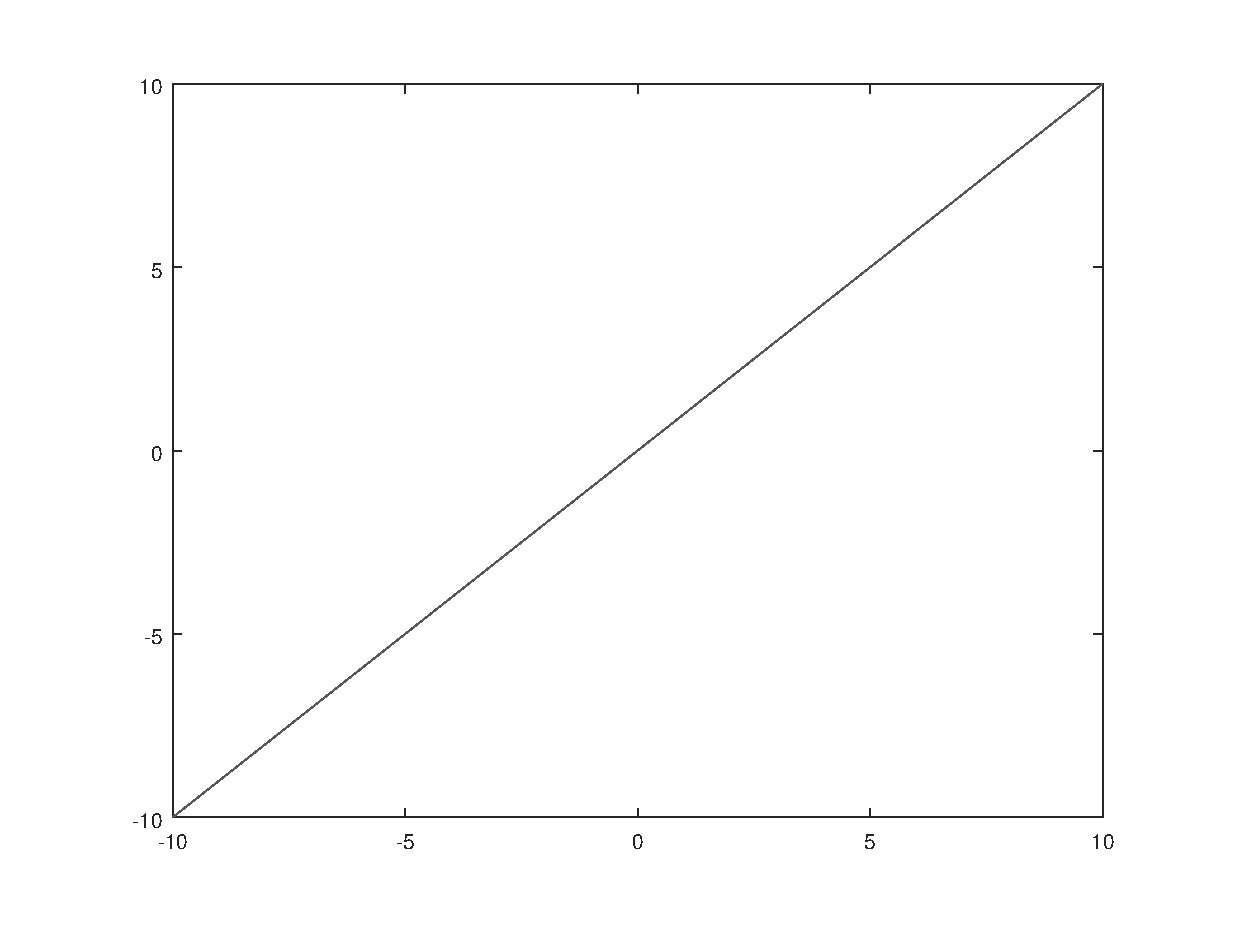
\includegraphics[width=0.9\linewidth]{img/grafica_recta.eps}
		\caption{Una recta.}
		\label{fig:sub_grafica_2}
	\end{subfigure}
	~ % No remover porque ocasionaría un salto de línea
	\begin{subfigure}[ht!]{.32\linewidth}
		\centering
		\includegraphics[width=0.9\linewidth]{img/grafica_parabola.eps}
		\caption{Una parábola.}
		\label{fig:sub_grafica_3}
	\end{subfigure}
	\caption{Tres gráficas de Octave.}
	\label{fig:tres_subfiguras}
\end{figure}

El código de la figura \ref{fig:tres_subfiguras} se muestra en el listado \ref{lst:tres_subfiguras}, donde podemos apreciar que el ancho de cada subfigura es del 32\% del ancho de línea (líneas 2, 9, y 16). Si incremento el tamaño al 33\%, las tres imágenes no caben en la misma línea.

Lo sé, lo sé, dos subfiguras al 50\% sí caben, pero tres al 33\% no... podemos discutir todo el día al respecto, o buscar la explicación pero, al final del día, lo más rápido es disminuir un poquito los porcentajes para que todo se vea bonito (de nuevo, uno no pelea con los flotantes, solo se adapta).

\begin{lstlisting}[style=latex,numbers=left,label=lst:tres_subfiguras,caption={Código para tres subfiguras.},
linebackgroundcolor={%
	\ifnum \value{lstnumber} =  2 \color{codigo_linea_resaltada}
	\else \ifnum \value{lstnumber} =  9 \color{codigo_linea_resaltada}
	\else \ifnum \value{lstnumber} = 16 \color{codigo_linea_resaltada}
	\else \color{codigo_fondo}
	\fi\fi\fi % Tantos \fi como líneas subrayadas.
}]
\begin{figure}[ht!]
	\begin{subfigure}[ht!]{.32\linewidth}
		\centering
		\includegraphics[width=0.9\linewidth]{img/grafica_seno.eps}
		\caption{Función seno.}
		\label{fig:sub_grafica_1}
	\end{subfigure}
	~ % No remover porque ocasionaría un salto de línea
	\begin{subfigure}[ht!]{.32\linewidth}
		\centering
		\includegraphics[width=0.9\linewidth]{img/grafica_recta.eps}
		\caption{Una recta.}
		\label{fig:sub_grafica_2}
	\end{subfigure}
	~ % No remover porque ocasionaría un salto de línea
	\begin{subfigure}[ht!]{.32\linewidth}
		\centering
		\includegraphics[width=0.9\linewidth]{img/grafica_parabola.eps}
		\caption{Una parábola.}
		\label{fig:sub_grafica_3}
	\end{subfigure}
	\caption{Tres gráficas de Octave.}
	\label{fig:figure_subfigure}
\end{figure}
\end{lstlisting}

Espero que con este ejemplo de subfiguras también te quede claro por qué \LaTeX{} no marca error al incluir varias |\caption| en un mismo entorno |figure|: hay usos legítimos que permiten este comportamiento.

Lo que el paquete |subfigure| hace es darnos una forma más fácil de trabajar con este comportamiento donde más de una etiqueta será necesaria dentro de un mismo entorno |figure|.

Y, en general, eso es lo que la mayoría de los paquetes hacen: encapsular la complejidad de \LaTeX{} con más entornos e instrucciones, para facilitarnos la vida a aquellos que no somos expertos en el tema pero deseamos hacer lo mismo.



\section*{Resumen}



En este capítulo aprendimos a ver las figuras en \LaTeX{} con nuevos ojos. Primero, aprendimos que la forma de referenciarlas el 99.9\% de las veces es a través de etiquetas y referencias.

Después, que las imágenes se incluyen gracias al paquete \texttt{graphicx}, y que se incluyen por referencia al nombre de archivo, generando peso en el documento de tesis hasta que se genera el PDF.

Investigamos varias opciones para lidiar con el tamaño de imagen, entre los que están \texttt{scale}, \texttt{width}, \texttt{height}, y \texttt{keepaspectratio}.

Finalmente, aprendimos a incluir subfiguras, que es lo mismo que decir que es una figura con varias figuritas bebé.

Pero aún queda otra especie de flotantes primitivos sin investigar: las tablas.
\lstDeleteShortInline|
\lstMakeShortInline[style=latexi]^

\chapter{Tablas}
\label{cha:tablas}



Hacer tablas en \LaTeX{} es una tarea que puede llevar mucho tiempo, incluso si ya comprendemos su funcionamiento. Para evitar tanto trabajo manual, y reducir la posibilidad de error, el enfoque para la creación de tablas que se recomienda en este capítulo (y que uso al crear mis documentos) es hacer uso de un editor de tablas en línea, para después modificar o corregir detalles.

Comenzaremos creando una tabla simple en el editor para después analizar su código instrucción a instrucción. Luego iremos agregando elementos a la tabla con el fin de tener el conocimiento para crear y modificar tablas sin depender de un editor.



\section{Generador de tablas}
\label{sec:generador_de_tablas}



El generador que yo utilizo reside en \href{https://www.tablesgenerator.com/}{https://www.tablesgenerator.com/}. Es un editor en línea, por lo que no requieres ninguna instalación adicional. La figura \ref{fig:table_editor} muestra la página principal, donde la barra de navegación superior muestra varios formatos en los que se pueden generar las tablas.

\begin{figure}[ht!]
	\centering
	\includegraphics[width=\linewidth]{img/table_editor_300ppi.png}
	\caption{Página principal del editor de tablas en línea.}
	\label{fig:table_editor}
\end{figure}

El primer paso para generar una tabla es comprobar que estamos trabajando en la pestaña de \LaTeX{}. Posteriormente, para lograr una tabla de $3\times3$ como se ve en la figura \ref{fig:table_editor}, se selecciona \opcionMenu{File $\rightarrow$ New table...} y se introducen los valores para filas y columnas en la nueva pantalla (figura \ref{fig:new_table}).

\begin{figure}[ht!]
	\centering
	\includegraphics[scale=0.80]{img/table_new_table_300ppi.png}
	\caption{Diálogo modal para nuevas tablas.}
	\label{fig:new_table}
\end{figure}

En la cuadrícula podemos rellenar cada una de las celdas dando clic sobre ellas para escribir el contenido. Posteriormente, se le puede dar formato. De momento, introduce los valores que se ven en la figura \ref{fig:table_gatito}, simulando una partida de \emph{gato}.

\begin{figure}[ht!]
	\centering
	\includegraphics[width=\linewidth]{img/table_gatito_300ppi.png}
	\caption{Contenido de nuestro primer ejemplo de tabla.}
	\label{fig:table_gatito}
\end{figure}

Tras introducir el contenido damos clic en el botón \opcionMenu{Generate}, ubicado debajo de la tabla que editamos, para generar el código \LaTeX{}, mismo que se ve en la figura \ref{fig:table_gatito_codigo}. Además, puedes copiar todo el código generado gracias al botón \opcionMenu{Copy to clipboard} en el lado derecho, para así colocarlo en Overleaf.

\begin{figure}[ht!]
	\centering
	\includegraphics[width=\linewidth]{img/table_gatito_codigo_300ppi.png}
	\caption{Código generado para nuestro primer ejemplo de tabla.}
	\label{fig:table_gatito_codigo}
\end{figure}

Ahora que hemos llegado al código generado, el resto del capítulo tendrá el código en listados para explicar las líneas relevantes, aunque dicho código proviene del editor en línea. Lo primero que tenemos que revisar es el entorno \texttt{table}.


\section{Entorno \texttt{table}}
\label{sec:entorno_table}


El código generado por el editor se muestra en el listado \ref{lst:primera_tabla}. Y, sí, en esta página puede que veas un ``gatito'' perdido en la esquina superior izquierda, ¿qué pasó?

Si recuerdas la sección de elementos flotantes (página \pageref{sub:elementos_flotantes}), mencioné que la tabla pertencía a esta categoría. Y justo la primera línea de la tabla generada en el listado \ref{lst:primera_tabla} muestra el indicador de posición en unos corchetes vacíos al crear un entorno \texttt{table}.

\begin{lstlisting}[style=latex,caption={Código de primera tabla generada.},label=lst:primera_tabla]
\begin{table}[]
	\begin{tabular}{lll}
	x & o & x \\
	o & x & o \\
	o & o & x
	\end{tabular}
\end{table}
\end{lstlisting}

\begin{table}[]
	\begin{tabular}{lll}
	x & o & x \\
	o & x & o \\
	o & o & x
	\end{tabular}
\end{table}

Como no existe el indicador \texttt{!}, ni el \texttt{h}, lo que sigue en la prioridad es una \texttt{t}, para ubicar el elemento flotante (el entorno \texttt{table}) en la parte superior de la página. Como también carecemos de la instrucción ^\centering^, la tabla aparece alineada a la izquierda, la posición predeterminada del texto en idioma español.

Para terminar, la tabla carece de una leyenda y, por lo tanto, de una etiqueta que nos permita hacer referencias posteriormente. En conclusión, una tabla puede tener los mismos cuatro elementos que la figura:
\begin{enumerate}
	\item Indicador de ubicación \texttt{ht!}, para ubicarla cerca de su posición en el código.
	\item La instrucción ^\centering^, para centrarla horizontalmente.
	\item Una leyenda para describir su propósito.
	\item Una etiqueta, para usar de referencia.
\end{enumerate}

El editor en línea tiene opciones adicionales para agregar casi todo lo anteriormente mencionado, pero primero acabaremos la explicación del código que ya tenemos.



\section{Entorno \texttt{tabular}}
\label{sec:entorno_tabular}



De la misma forma en la que el entorno \texttt{figure} solo envolvía un \texttt{picture} o un ^\includegraphics^, el entorno \texttt{table} sirve solamente para generar la leyenda y la etiqueta, pero la acción de verdad pasa en el entorno \texttt{tabular}.

El entorno \texttt{tabular} comienza en la segunda línea en el listado \ref{lst:primera_tabla}, y recibe un argumento obligatorio (el valor entre llaves) que determina la alineación de cada una de las columnas presentes en la tabla.

Es decir, si decides eliminar por completo este argumento, dejando solamente

\begin{lstlisting}[style=latex,numbers=none]
\begin{tabular}
\end{lstlisting}

\noindent tendrás bastantes errores con los cuales lidiar:

\begin{lstlisting}[style=errores]
LaTeX Error: Illegal character in array arg. [	x]
Extra alignment tab has been changed to \cr. [	x &]
Extra alignment tab has been changed to \cr. [	x & o &]
Extra alignment tab has been changed to \cr. [	o &]
Extra alignment tab has been changed to \cr. [	o & x &]
Extra alignment tab has been changed to \cr. [	o &]
Extra alignment tab has been changed to \cr. [	o & o &]
\end{lstlisting}

Sí, todo un desastre aunque solo quitamos el argumento requerido para el entorno \texttt{tabular}. Únicamente recuerda: si en alguna tabla tienes errores similares, siempre revisa que el argumento esté presente.

No obstante, su sola presencia no basta porque tiene que coincidir con el número de columnas. De lo contrario, si dejamos solamente dos (en este ejemplo), con

\begin{lstlisting}[style=latex,numbers=none]
\begin{tabular}{ll}
\end{lstlisting}

\noindent aún tenemos una parte de los errores que salieron cuando removimos completamente el argumento:

\begin{lstlisting}[style=errores]
Extra alignment tab has been changed to \cr. [	x & o &]
Extra alignment tab has been changed to \cr. [	o & x &]
Extra alignment tab has been changed to \cr. [	o & o &]
\end{lstlisting}

De cualquier forma, el generador hace el conteo de columnas por nosotros y coloca bien la cantidad, así que este conocimiento nos es útil para modificar después si es necesario. Tres columnas, tres letras...

¿Pero por qué \texttt{l}? Para especificar alineación a la izquierda, del inglés \emph{left}. Podemos usar al menos los siguientes tres valores:
\begin{itemize}
	\item \texttt{l}, para alinear a la izquierda,
	\item \texttt{c}, para alinear al centro, y
	\item \texttt{r}, del inglés \emph{right}, para alinear a la derecha.
\end{itemize}

Lo que resta de contenido, las líneas:

\begin{lstlisting}[style=latex,numbers=none]
x & o & x \\
o & x & o \\
o & o & x
\end{lstlisting}

\noindent corresponden a cada una de las filas en la tabla, con cada una de sus tres columnas. ¿Cómo separamos una línea de la otra? Con la instrucción \codigo{\textbackslash{}} al final de la línea. ¿Y cómo se separan las columnas? Con el símbolo \texttt{\&}.

Al editar tablas manualmente tenemos que garantizar que la cantidad de \emph{ampersand} (\texttt{\&}) por fila sea de \texttt{columnas - 1} (se necesitan dos ampersand parar generar tres columnas), y que el argumento del entorno \texttt{tabular} contenga \texttt{columnas} indicadores de alineación (tres columnas, tres letras de alineación).



\section{Generador: opciones adicionales}
\label{sec:generador_opciones_adicionales}



Podemos agregarle a una tabla los mismos elementos que a una figura, desde el generador en línea. Debajo del código producido existe un pequeño \emph{combobox}\footnote{Elemento de la interfaz con una flechita a la derecha, que permite seleccionar varias opciones.} que permite agregar la leyenda y la instrucción de centrado (figura \ref{fig:table_editor_extra_options}). Siguiendo con el formato del libro, colocaremos la leyenda debajo, seleccionando \opcionMenu{Caption below}, y agregaremos la instrucción de centrado horizontal eligiendo \opcionMenu{Center table horizontally}.

\begin{figure}[ht!]
	\centering
	\includegraphics[width=\linewidth]{img/table_editor_extra_options_300ppi.png}
	\caption{Opciones adicionales para la tabla.}
	\label{fig:table_editor_extra_options}
\end{figure}

Tras seleccionar estas dos opciones, el \emph{combobox} se actualizará al valor \texttt{Caption below, center table horizontally}, y agregará dos cajas de texto a la interfaz, sobre el código: una para colocar la leyenda (caja de \texttt{Table caption}) y otra para la etiqueta (caja de \texttt{label}). La interfaz actualiza tras estos cambios se muestra en la figura \ref{fig:table_editor_caption}.

\begin{figure}[ht!]
	\centering
	\includegraphics[width=\linewidth]{img/table_editor_caption_300ppi.png}
	\caption{Caja de texto para introducir leyenda y etiqueta.}
	\label{fig:table_editor_caption}
\end{figure}

Lo único que el generador no permite agregar es el indicador de ubicación, el valor entre corchetes del entorno \texttt{table}. No obstante, como se comporta de manera similar a una figura, utilizamos el indicador \texttt{ht!}. El código nuevo generado, más la ubicación de la tabla, se muestra en el listado \ref{lst:tabla_leyenda}.

\begin{lstlisting}[style=latex,caption={Código para tabla con leyenda.},label=lst:tabla_leyenda]
\begin{table}[ht!]
	\centering
	\begin{tabular}{lll}
		x & o & x \\
		o & x & o \\
		o & o & x
	\end{tabular}
	\caption{Primera tabla, con leyenda.}
	\label{tab:primera_tabla_leyenda}
\end{table}
\end{lstlisting}

Dado que ya tiene una leyenda y una etiqueta, podemos referenciar la tabla mediante un ^\ref{tab:primera_tabla_leyenda}^, similar a una figura. Por lo tanto, ya podemos decir que el código del listado \ref{lst:tabla_leyenda} da como resultado la tabla \ref{tab:primera_tabla_leyenda}.

\begin{table}[ht!]
	\centering
	\begin{tabular}{lll}
		x & o & x \\
		o & x & o \\
		o & o & x
	\end{tabular}
	\caption{Primera tabla con leyenda.}
	\label{tab:primera_tabla_leyenda}
\end{table}



\section{Bordes}
\label{sec:bordes}



Ya que tenemos el contenido, ¿dónde está la rejilla que me permite saber que estoy jugando gato? ¿Cómo colocamos los bordes de las celdas?

Esto tiene dos respuestas, porque depende si quieres bordes entre columnas o bordes entre filas. Para colocar los bordes entre columnas se utiliza el símbolo de línea vertical (\texttt{|}) junto con el argumento de la alineación del entorno \texttt{tabular}. Es decir, si queremos borde entre las columnas 1 y 2, y entre las columnas 2 y 3, el nuevo valor de dicho algumento es \texttt{\{l | l | l\}} (con espacios solo para mejor estética en el código).

Pero si queremos una línea que separe las filas 1 y 2, y las filas 2 y 3, es necesario usar la instrucción ^\hline^ al terminar el renglón. El código del listado \ref{lst:tabla_bordes} genera la tabla que se muestra en la columna derecha:

\noindent \begin{minipage}[ht!]{.80\linewidth}
% Aparentemente, no se pueden meter floats a un minipage,
% por eso no puedo tener mi table dentro de estas dos columnas.
\begin{lstlisting}[style=latex,frame={},caption={Código de tabla con bordes.},label=lst:tabla_bordes]
\begin{tabular}{l|l|l}
	x & o & x \\ \hline
	o & x & o \\ \hline
	o & o & x
\end{tabular}
\end{lstlisting}
\end{minipage}
\begin{minipage}[ht!]{.19\linewidth}
\begin{center}
	\vspace{-0.7cm}
	\begin{tabular}{l|l|l}
		x & o & x \\ \hline
		o & x & o \\ \hline
		o & o & x
	\end{tabular}
\end{center}
\end{minipage}

No obstante, ¿qué pasa si no queremos un borde que cubra de lado a lado, o de arriba a abajo, completamente? En el caso de las filas, sustituimos la instrucción ^\hline^ por una ^\cline^, seguida del rango de columnas que tendrá borde.

Por ejemplo, digamos que queremos que el borde inferior de la primera fila del gato cubra únicamente las columnas 1 y 2, y el borde inferior de la segunda fila solo las columnas 1 y 3. En el primer caso, una instrucción ^\cline{1-2}^ cubrirá lo necesario, pero para el segundo caso serán necesarias dos instrucciones separadas: ^\cline{1-1}^ y ^\cline{3-3}^ (nótese que se utiliza un rango aunque la línea vaya a cubrir una sola celda).

La tabla con estos nuevos bordes se crea en el listado \ref{lst:table_uneven_row_borders}, aunque también se puede generar con el editor en línea seleccionando los bordes deseados con la opción \opcionMenu{Custom Grid Edit}, botón que se encuentra resaltado en naranja en la figura \ref{fig:table_borders}. Ya eligirás tú si prefieres escribir el código o dar clic en los bordes correspondientes.

\begin{figure}[ht!]
	\centering
	\includegraphics[width=\linewidth]{img/table_borders_300ppi.png}
	\caption{Edición de bordes con editor en línea.}
	\label{fig:table_borders}
\end{figure}

\noindent \begin{minipage}[ht!]{.80\linewidth}
\begin{lstlisting}[style=latex,frame={},caption={Código de tabla con bordes incompletos para filas.},label=lst:table_uneven_row_borders]
\begin{tabular}{l|l|l}
	x & o & x \\ \cline{1-2}
	o & x & o \\ \cline{1-1} \cline{3-3}
	o & o & x
\end{tabular}
\end{lstlisting}
\end{minipage}
\begin{minipage}[ht!]{.19\linewidth}
\begin{center}
	\vspace{-0.7cm}
	\begin{tabular}{l|l|l}
		x & o & x \\ \cline{1-2}
		o & x & o \\ \cline{1-1} \cline{3-3} 
		o & o & x
	\end{tabular}
\end{center}
\end{minipage}

¿Cómo colocamos bordes a solo una parte de la columna? En términos del generador en línea, sigue siendo cosa de manualmente elegir con el ratón cada borde. En código... es una nueva instrucción por cada celda con borde entre columnas.

Lo primero que hay que hacer para establecer bordes laterales parciales es remover el borde del indicador del entorno \texttt{tabular}. Después de eso, cada celda con borde lateral debe ser sustituida de su simple contenido (la \texttt{o} u \texttt{x} en el ejemplo) a una instrucción ^\multicolumn^ con el siguiente formato:

\begin{lstlisting}[style=latex,numbers=none]
\multicolumn{1}{alineación y bordes}{contenido}
\end{lstlisting}

Por ejemplo, si en la primera fila queremos conservar solamente el borde a la derecha de la \texttt{o}, sustituimos con un ^\multicolumn{1}{l|}{o}^ (si fuera a la izquierda, sería un ^\multicolumn{1}{|l}{o}^). En la segunda fila no habrá bordes, y en la tercera línea colocamos bordes a ambos lados de la \texttt{o} central. El código generado se muestra en el listado \ref{lst:table_uneven_col_borders}.

\noindent \begin{minipage}[ht!]{.80\linewidth}
\begin{lstlisting}[style=latex,frame={},caption={Código de tabla con bordes incompletos para columnas.},label={lst:table_uneven_col_borders}]
\begin{tabular}{lll}
x                      & \multicolumn{1}{l|}{o} & x \\
\cline{1-2}
o                      & x                      & o \\
\cline{1-1} \cline{3-3}
\multicolumn{1}{l|}{o} & \multicolumn{1}{l|}{o} & x
\end{tabular}
\end{lstlisting}
\end{minipage}
\begin{minipage}[ht!]{.19\linewidth}
\begin{center}
	\vspace{-0.7cm}
	\begin{tabular}{lll}
		x                      & \multicolumn{1}{l|}{o} & x \\ \cline{1-2}
		o                      & x                      & o \\ \cline{1-1} \cline{3-3} 
		\multicolumn{1}{l|}{o} & \multicolumn{1}{l|}{o} & x
	\end{tabular}
\end{center}
\end{minipage}

Sí, sé que te lo preguntas: ¿por qué el generador puso los bordes en dos celdas distintas si pudimos haber puesto los dos bordes sobre una misma celda? Como quizá sospechas, las instrucciones

\begin{lstlisting}[style=latex,numbers=none]
\multicolumn{1}{l|}{o} & \multicolumn{1}{l|}{o} & x
\end{lstlisting}

\noindent y

\begin{lstlisting}[style=latex,numbers=none]
o & \multicolumn{1}{|l|}{o} & x
\end{lstlisting}

\noindent son equivalentes. Ya será cuestión de preferencias el cómo decides redactar el código, mientras el objetivo se logre.


\section{Centrado de encabezados}
\label{sec:centrado_de_encabezados}



Para el centrado de encabezados se utiliza la misma instrucción que para colocar bordes individuales: ^\multicolumn^. Para centrar, o cambiar la alineación respecto al parámetro global del \texttt{tabular}, se utiliza el indicador de alineación. Por ejemplo, para la tabla \ref{tab:instrucciones_de_secciones} (pp.\pageref{tab:instrucciones_de_secciones}) se utilizó el código que se muestra en el listado \ref{lst:table_ubicacion}.

\begin{lstlisting}[style=latex,numbers=left,caption={Código de tabla de indicadores de ubicación.},label={lst:table_ubicacion},
linebackgroundcolor={%
	\ifnum \value{lstnumber} =  5 \color{codigo_linea_resaltada}
	\else \color{codigo_fondo}
	\fi % Tantos \fi como líneas subrayadas.
}]
\begin{table}[ht]
\centering
\begin{tabular}{cl}
\hline
\textbf{Parámetro} & \multicolumn{1}{c}{\textbf{Posición}}
\\
\hline
\texttt{h}         & Aquí... por favor, y si es posible.                           \\
\texttt{t}         & En la parte superior de la página (del inglés \emph{top}).    \\
\texttt{b}         & En la parte inferior de la página (del inglés \emph{bottom}). \\
\texttt{p}         & Colocar en una página especial para flotantes.                \\
\texttt{!}         & Ignorar los parámetros que \LaTeX{} considera buenos.         \\
\texttt{H}         & Sin comentarios...                                            \\
\hline
\end{tabular}
\caption{Posibles valores del indicador de ubicación.} % Leyenda de la tabla.
\label{tab:indicador_ubicacion}
\end{table}
\end{lstlisting}

La línea de nuestro interés en el listado \ref{lst:table_ubicacion} es la 5,

\begin{lstlisting}[style=latex,numbers=none]
\textbf{Parámetro} & \multicolumn{1}{c}{\textbf{Posición}}
\end{lstlisting}

\noindent donde se utiliza la instrucción ^\multicolumn^ para producir el título \emph{Posición} centrado, con el resto del contenido en la columna alineado a la izquierda. El segundo par de llaves en esa instrucción es lo que nos interesa. Tuvimos que escribir todo el ^\multicolumn^, con sus tres pares de llaves, solo para cambiar una \texttt{l}, definida en el entorno \texttt{tabular}, por una \texttt{c}, definida a nivel celda.

Aprovechando la ocasión del desastre que parece el listado \ref{lst:table_ubicacion}, hablemos de uno de los problemas de editar tablas en \LaTeX{}: editar a mano es un dolor de cabeza por el espacio en blanco. En el listado, las líneas 8, 9, 10... bueno, todas las líneas con contenido en los renglones tuvieron que expandirse a dos debido a su longitud por espacio en blanco. No obstante, al editar sin separar las líneas por ancho de página, el código luce como en la figura \ref{fig:codigo_tabla_espacio}, con un orden visual tranquilizador.

El problema es que, con solo dos columnas, ya ocupamos casi todo el espacio disponible para una línea en el monitor, gracias a los encabezados centrados que demandan tanto espacio en términos de caracteres... pero la opción es editar sin alinear columnas y tener que buscar los ampersand para saber dónde tenemos que editar a mano.

De cualquier forma, pierdes: o tienes mucho espacio vacío y la necesidad de usar barra desplazadora, o tienes todo compacto pero sin un apoyo visual que te diga dónde están las columnas. O lo peor de ambos mundos\footnote{Te he fallado, Hannah Montana :(.}, lo que ocurrió en el listado \ref{lst:table_ubicacion} por su necesidad de ser una página impresa: mucho espacio vacío, con líneas separadas para no exceder los márgenes del documento, lo que te quita la habilidad de ver fácilmente dónde están las columnas.

\begin{figure}[ht!]
	\centering
	\includegraphics[width=\linewidth]{img/table_code_space.png}
	\caption{Editando código de tabla en ancho fijo, sin separar líneas.}
	\label{fig:codigo_tabla_espacio}
\end{figure}



\section{Combinación de columnas}
\label{sec:combinacion_de_columnas}



Después de haberla utilizado para bordes y centrar un encabezado, por fin vamos a darle el uso legítimo a la instrucción ^\multicolumn^. Resulta que se llama así porque sirve para hacer que una celda se expanda a múltiples columnas (del inglés \emph{multiple column}). Unir celdas horizontalmente, pues. Y, sí, justo ese primer parámetro, ese \texttt{1} olvidado, es la cantidad de columnas que esta nueva multicolumna debe abarcar dentro de la fila.

\begin{table}[ht]
\centering
\begin{tabular}{l|rrr}
\hline
\multicolumn{4}{c}{\textbf{Calificaciones de 4A}} \\ \hline
Carlos         & 4         & 8         & 4        \\
Ixchel         & 10        & 9         & 8        \\
Abimael        & 9         & 10        & 10       \\ \hline
\end{tabular}
\caption{Tabla con columnas unidas.}
\label{tab:calificaciones}
\end{table}

La tabla \ref{tab:calificaciones} tiene un encabezado que se expande a lo largo de las cuatro columnas, longitud que se indica en la línea 5 del listado \ref{lst:tabla_calificaciones} con el primer parámetro entre llaves. En esta línea ya no utilizamos más ampersands\footnote{Sí, en español se supone que se llama \textbf{et}... la costumbre.} (\&) porque la multicolumna se encarga de representar todas las columnas.

\begin{lstlisting}[style=latex,numbers=left,caption={Tabla con encabezado de cuatro columnas de ancho.},label={lst:tabla_calificaciones},
linebackgroundcolor={%
	\ifnum \value{lstnumber} =  5 \color{codigo_linea_resaltada}
	\else \color{codigo_fondo}
	\fi % Tantos \fi como líneas subrayadas.
}]
\begin{table}[ht]
\centering
\begin{tabular}{l|rrr}
\hline
\multicolumn{4}{c}{\textbf{Calificaciones de 4A}} \\ \hline
Carlos         & 4         & 8         & 4        \\
Ixchel         & 10        & 9         & 8        \\
Abimael        & 9         & 10        & 10       \\ \hline
\end{tabular}
\caption{Tabla con columnas unidas.}
\label{tab:calificaciones}
\end{table}
\end{lstlisting}



\section{Combinación de filas	}
\label{sec:combinacion_de_filas}


Supongamos ahora que debemos incluir una tabla que necesita agrupar un conjunto de filas. Por ejemplo, la tabla \ref{tab:estados_norte} muestra un extracto de los estados de México agrupados por zona. ¿Cómo fue hecha?

\begin{table}[ht]
\centering
\begin{tabular}{ll}
\hline
\multicolumn{1}{c}{\textbf{Zona}} & \multicolumn{1}{c}{\textbf{Estado}}
\\ \hline
\multirow{4}{*}{Norte}            & Chihuahua                           \\
                                  & Durango                             \\
                                  & Coahuila                            \\
                                  & Nuevo León                          \\ \hline
\end{tabular}
\caption{Ejemplo de tabla con \texttt{multirow}.}
\label{tab:estados_norte}
\end{table}

Para la combinación de filas requerimos de un paquete adicional: \texttt{multirow}. Este paquete nos dará la habilidad de usar la instrucción ^\multirow^, que tiene un formato similar a ^\multicolumn^:

\begin{lstlisting}[style=latex,numbers=none]
\multirow{número de filas}{alto}{contenido de las celdas}
\end{lstlisting}

El listado \ref{lst:tabla_estados} nos muestra un ejemplo de tabla con celda multifila. La línea 7 crea una celda de cuatro filas de alto (según su primer parámetro) y tiene el contenido de \emph{Norte} (según el tercer par de llaves). La estrella (\texttt{*}) en el segundo parámetro sirve para indicarle al compilador que debe calcular automáticamente la altura de la celda en base a la cantidad de filas sobre las cuales se expande. Esto con el fin centrar verticalmente el contenido.

Pero, entonces, ¿cómo se cambia la alineación horizontal de una fila que se expande a lo alto de cuatro filas? Justo como lo hicimos para una sola celda, usando ^\multicolumn^. Si quieres más detalles sobre cómo utilizar una multicolumna con una multifila puedes consultar \cite{bib:multicol_multirow}.

\begin{lstlisting}[style=latex,numbers=left,caption={Tabla con columna de cuatro filas de alto.},label={lst:tabla_estados},
linebackgroundcolor={%
	\ifnum \value{lstnumber} =  7 \color{codigo_linea_resaltada}
	\else \color{codigo_fondo}
	\fi % Tantos \fi como líneas subrayadas.
}]
\begin{table}[ht]
\centering
\begin{tabular}{ll}
\hline
\multicolumn{1}{c}{\textbf{Zona}}&\multicolumn{1}{c}{\textbf{Estado}}
\\ \hline
\multirow{4}{*}{Norte} & Chihuahua  \\
                       & Durango    \\
                       & Coahuila   \\
                       & Nuevo León \\ \hline
\end{tabular}
\caption{Ejemplo de tabla con \texttt{multirow}.}
\label{tab:estados_norte}
\end{table}
\end{lstlisting}

También puedes modificar otras cosas estéticas de la tabla, como el ancho de los bordes o los colores de fondo. No obstante, hasta aquí llega lo básico que necesitas para tu tesis. Si requieres estos cambios en el formato de una tabla, consulta \cite{bib:overleaf_tables}.



\section*{Resumen}



En este capítulo vimos que la mejor forma de trabajar con las tablas en \LaTeX{} es dejando que un generador las haga por nosotros. Aún así, analizamos el código necesario para codificar tablas de manera manual, en el no-tan-deseado caso de tener que hacer modificaciones sin ayuda del generador.

Estos cambios incluyen modificar el contenido de la celda, cambiar la alineación, colocar bordes, crear celdas multicolumna, y celdas multifila.

Ahora que hemos visto cómo incluir tablas, viene algo que promete ser aún más divertido: ecuaciones.

\lstDeleteShortInline^
\lstMakeShortInline[style=latexi]|
\lstDeleteShortInline|
\lstMakeShortInline[style=latexi]!

\chapter{Ecuaciones}
\label{cha:ecuaciones}



Aquí es donde separamos las tesis de ingeniería de las tesis de otras carreras: las hermosas matemáticas (que merecen una tipografía para hacerles justicia). Hace mucho tiempo, Word fallaba miserablemente para esto de las ecuaciones (ya ha mejorado bastante), y la única alternativa digna era utilizar \LaTeX{}. En fin.

En este capítulo veremos que la diversidad de entornos matemáticos que \LaTeX{} ofrece, junto con la irrisoria cantidad de símbolos y la facilidad con la que podemos escribir ecuaciones (cuando sabemos cómo), brindan a \LaTeX{} un triunfo devastador sobre su contrincante Word.

Vayamos a descubrir las posibilidades que \LaTeX{} nos ofrece, ya sea que necesitemos ecuaciones de álgebra booleana, evaluación de derivadas, álgebra lineal, expresiones de probabilidad... \LaTeX{} nos ofrece con abundancia.



\section{Ecuaciones en línea con el texto}
\label{sec:ecuaciones_en_linea}



La forma más fácil de introducir ecuaciones en \LaTeX{} es incluirlas en el mismo texto, mediante un entorno que abre y cierra con símbolos de pesos (\texttt{\$}). Por ejemplo, si quiero hablar de la variable $x$, uso este entorno. Porque no es lo mismo una ``x'' de texto que una $x$ de matemáticas: cambia la fuente.

Dicho de otra forma, yo puedo hablar de las variables $x$ y $y$ porque un entorno matemático tiene una fuente diferente que me permite distinguir qué cosas son matemáticas dentro del texto.

Si escribo la ecuación de la recta, $y = mx + b$, fácilmente puedo ver dónde está la ecuación. Y no, no es lo mismo la fuente del entorno matemático al estilo en itálicas: $y = mx + b$ contra \emph{y = mx + b}. Por ejemplo, tenemos $=$ e \emph{=}; $+$ y \emph{+}; $b$ y \emph{b}. No dejes que las letras te engañen, son los símbolos matemáticos los que hacen la diferencia.

No obstante, allí es donde acaban las similitudes. Porque ahora tenemos que evaluar el primer punto de la recta, $y_1$ (cuyo código es !$y_1$!). ¿Cómo colocas ese subíndice en texto en itálicas?

Ahora por fin comprendes por qué \LaTeX{} tiene conflictos con los guiones bajos: son un símbolo que indica que el siguiente carácter es un subíndice. Cuando esta instrucción se hace fuera de un entorno matemático, \LaTeX{} no sabe qué hacer y genera un error.

Esto es solo el principio. Podemos colocar varios caracteres como subíndice, con rodear el texto entre llaves, como en $y_{312}$ (cuyo código es !$y_{312}$!).

Colocar un exponente es igual de trivial, con el uso del símbolo de intercalación, circunflejo, o ``gorrito'' (\^{}). Por ejemplo, una parábola en su forma general se define por $Ax^2 + Bxy + Cy^2 + Dx + Ey + F = 0$, lo cual escribimos en código en línea como !$Ax^2 + Bxy + Cy^2 + Dx + Ey + F = 0$!.

A la hora de querer evaluar el valor del doceavo punto dentro de esa fórmula general basta con agregar los subíndices, sin importar si va primero exponente o subíndice: $Ax^2_{12} + Bx_{12}y_{12} + Cy_{12}^2 + Dx_{12} + Ey_{12} + F = 0$. El código es:

\begin{lstlisting}[style=latex,mathescape=false]
$Ax^2_{12} + Bx_{12}y_{12} + Cy_{12}^2 + Dx_{12} + Ey_{12} + F = 0$
\end{lstlisting}



\section{Letras griegas y otros símbolos}
\label{sec:letras_griegas_y_otros_simbolos}



Por supuesto, las matemáticas no son matemáticas si la $x$ no invita a todas sus compañeras de la Antigua Grecia al baile. Están las más conocidas y queridas, como $\alpha$ (!$\alpha$!), $\beta$ (!$\beta$!), y $\pi$ (!$\pi$!), y también otras conocidas pero odiadas, como $\Sigma$ (!$\Sigma$!). ¿Y cómo olvidar que para llegar a un resultado tenemos que colocar los tres puntitos del ``por lo tanto'' ($\therefore$, !$\therefore$!)?

Por cierto, el símbolo $\therefore$ forma parte del paquete \texttt{amssymb}, por lo que debes verificar que esté presente en el preámbulo. De lo contrario, tendrás el siguiente error:

\begin{lstlisting}[style=errores]
Undefined control sequence. [...puntitos del ``por lo tanto'' ($\therefore]
\end{lstlisting}

Es importante mencionar que $\sigma$ (!$\sigma$!) y $\Sigma$ (!$\Sigma$!) son dos instrucciones diferentes, lo que aplica para aquellas letras del abecedario que tienen una mayúscula que no se incluye en nuestro alfabeto contemporáneo de uso común (la mayúscula de $\alpha$ es $A$).

Si quieres usar \LaTeX{} para la teoría de conjuntos, se puede. Podemos poner la intersección de $A$ y $B$ con $A \cap B$ (!$A \cap B$!), o su unión con $A \cup B$ (!$A \cup B$!). Si $A = \{1, 3, 5\}$, y $B = \{1, 3, 5, 7\}$, entonces $A \subseteq B$ (!$A \subseteq B$!).

¿Y las matemáticas discretas usadas ampliamente en electrónica digital? Si representamos la operación \texttt{AND} como una multiplicación que se hace al estar juntas las variables, \texttt{OR} con un signo de $+$, y \texttt{NOT} con una línea sobre el texto, podemos entender que $x = \overline{\overline{AB} + A\overline{C}D}$ es una expresión válida, cuyo código es:

\begin{lstlisting}[style=latex,numbers=none,mathescape=false]
$x = \overline{\overline{AB} + A\overline{C}D}$
\end{lstlisting}

Antes de perderme en más ejemplos, el punto es que \LaTeX{} tiene el símbolo que necesitas. Puedes consultar \cite{bib:math_symbols} para una lista de las letras en el alfabeto griego, y \cite{bib:math_symbols_subject} para más símbolos agrupados por asignatura. Como dije, hay muchos.



\section{Ecuaciones sin referencia}
\label{sec:ecuaciones_sin_referencia}



Llega un momento en la vida en el que las ecuaciones son tan complejas para caber en línea con el texto y es necesario emigrar a lugares con más espacio. El siguiente entorno, o modo, lo llamaré ``entorno matemático sin referencia''. Es decir, es un entorno que ya nos asigna una línea completa para la ecuación, que centra el contenido, pero que no nos permite asignar una etiqueta para referencia.

Como ejemplo de este entorno tenemos la paradoja de la dicotomía de Zenón, que es la sucesión infinita que converge a 1:

\[
\frac{1}{2} + \frac{1}{4} + \frac{1}{8} + \frac{1}{16} + \frac{1}{32} + \ldots = \sum_{n=1}^{\infty} \left(\frac{1}{2}\right)^n = 1
\]

El código de la sucesión anterior es:

\begin{lstlisting}[style=latex,numbers=none,mathescape=false]
\[
\frac{1}{2} + \frac{1}{4} + \frac{1}{8} + \frac{1}{16} + \frac{1}{32} + \ldots = \sum_{n=1}^{\infty} \left(\frac{1}{2}\right)^n = 1
\]
\end{lstlisting}

Es decir, el entorno matemático sin referencia abre con un \codigo{[} y cierra con un \codigo{]}. Esto automáticamente crea una línea nueva para la ecuación y centra su contenido. En sí, la (casi) única instrucción que utilizamos fue !\frac{numerador}{denominador}!. Dicha instrucción es un ejemplo de la diferencia entre ecuaciones en línea con el texto y el entorno independiente: el mismo !\frac{1}{2}! se muestra más pequeño ($\frac{1}{2}$) en el texto.

Lo demás fueron dos nuevos símbolos: $\sum$ (!$\sum$!) e $\infty$ (!$\infty$!). Nótese que \LaTeX{} colocó automáticamente los límites debajo y encima del símbolo de sumatoria, en lugar de como subíndices y exponentes.

Lo que nos queda por ver es ¿por qué usamos !\left(! y !\right)!?



\section{Llaves y paréntesis}
\label{sec:llaves_y_parentesis}



La respuesta más simple viene de forma empírica. Este es el resultado al remover !\left! y !\right! de la ecuación pasada:

\[
\frac{1}{2} + \frac{1}{4} + \frac{1}{8} + \frac{1}{16} + \frac{1}{32} + \ldots = \sum_{n=1}^{\infty} (\frac{1}{2})^n = 1
\]

¿La diferencia? Sin el modificador, los paréntesis no se agrandan para cubrir completamente la fracción. La lección: en entornos matemáticos, acostumbra a colocar !\left(! y !\right)! a los símbolos de apertura y clausura que utilices. Esto incluye paréntesis, llaves, corchetes, barras verticales, y otros símbolos más, que puedes consultar en \cite{bib:math_brackets}.

En caso de querer modificar manualmente el tamaño de los paréntesis, tienes cuatro modificadores de tamaño, que se muestran en la tabla \ref{tab:math_corchetes}.

\begin{table}[ht]
\centering
\begin{tabular}{ll}
\hline
\multicolumn{1}{c}{\textbf{La instrucción...}} & \multicolumn{1}{c}{\textbf{se ve...}} \\
\hline
!\big(!                        & $1 + \big( \frac{1}{2} \big)$         \\
!\Big(!                        & $1 + \Big( \frac{1}{2} \Big)$         \\
!\bigg(!                       & $1 + \bigg( \frac{1}{2} \bigg)$       \\
!\Bigg(!                       & $1 + \Bigg( \frac{1}{2} \Bigg)$       \\
\hline
\end{tabular}
\caption{Tamaños de paréntesis en \LaTeX.}
\label{tab:math_corchetes}
\end{table}



\section{Ecuaciones con referencia}
\label{sec:ecuaciones_con_referencia}



Si quieres hacer referencia a una ecuación, como a la ecuación (\ref{eq:sucesion}), es necesario usar el entorno \texttt{equation}, como se muestra en el listado \ref{lst:entorno_equation}. Lo demás se mantiene igual, creas una etiqueta con !\label! y después la utilizas con !\ref!.

\begin{equation}
\frac{1}{2} + \frac{1}{4} + \frac{1}{8} + \frac{1}{16} + \frac{1}{32} + \ldots = \sum_{n=1}^{\infty} \left(\frac{1}{2}\right)^n = 1
\label{eq:sucesion}
\end{equation}

No obstante, usar la instrucción !\ref{eq:sucesion}! retorna únicamente el número de la ecuación, no los paréntesis. Ya dependerá de tu plantilla, o de tu institución, si debes agregar paréntesis a cada referencia a ecuación, o si así sin uso de paréntesis es el modo de referencia adecuado.

A lo largo de este capítulo, yo agrego los paréntesis de forma manual, escribiendo !(\ref{eq:sucesion})! para obtener la referencia con paréntesis.

\begin{lstlisting}[style=latex,caption={Código para ecuación con referencia.},label=lst:entorno_equation]
\begin{equation}
\frac{1}{2} + \frac{1}{4} + \frac{1}{8} + \frac{1}{16} + \frac{1}{32} + \ldots = \sum_{n=1}^{\infty} \left(\frac{1}{2}\right)^n = 1
\label{eq:sucesion}
\end{equation}
\end{lstlisting}



\section{Texto en entorno matemático}
\label{sec:texto_en_entorno_matematico}



Si por alguna razón debes escribir texto ``normal'' dentro de un entorno matemático, debes recordar que la fuente cambió y puede no tener todos los símbolos disponibles. Por ejemplo, la ecuación (\ref{eq:dolares}) muestra la tasa de cambio entre dólares y pesos... pero no se ve muy bien. La fuente es el primero de los problemas, dado que las cursivas no es un formato deseado para el texto.

\begin{equation}
tasa_{MXN} = \frac{pesos}{dólares} = \frac{2,968.24 MXN}{150 USD} \approx 19.78
\label{eq:dolares}
\end{equation}

El segundo problema es que ``dólares'' contiene una \texttt{ó} y no se puede desplegar con la fuente del entorno matemático, por lo que arroja la adevertencia:

\begin{lstlisting}[style=advertencias]
Command \' invalid in math mode on input line 159.
\end{lstlisting}

Para resolver este problema podemos utilizar !\mbox!, que permite mostrar texto en fuente del documento dentro del espacio matemático. Agregando !\mbox!, como se muestra en el listado \ref{lst:entorno_equation2}, se obtiene la ecuación (\ref{eq:dolares2}).

\begin{equation}
\mbox{tasa}_{\mbox{MXN}} = \frac{\mbox{pesos}}{\mbox{dólares}} = \frac{2,968.24 \mbox{MXN}}{150 \mbox{USD}} \approx 19.78
\label{eq:dolares2}
\end{equation}

En la ecuación ya se puede observar la fuente regular y la ``ó'' en la palabra ``dólares''. No obstante, queda un problemita más: no existe espacio entre el monto y la moneda (entre el número y el texto ``MXN'' o ``USD'') a pesar de que en el código sí aparece.

\begin{lstlisting}[style=latex,caption={Código con texto usando \texttt{\textbackslash{}mbox}.},label=lst:entorno_equation2]
\begin{equation}
\mbox{tasa}_{\mbox{MXN}} = \frac{\mbox{pesos}}{\mbox{dólares}} = \frac{2,968.24 \mbox{MXN}}{150 \mbox{USD}} \approx 19.78
\label{eq:dolares2}
\end{equation}
\end{lstlisting}

Esto es porque \LaTeX{} es aún más estricto con el espacio en blanco en los entornos matemáticos y simplemente elimina todo. Para mostrar espacios tenemos dos alternativas: o agregar el espacio dentro del !\mbox!, como !\mbox{ MXN}!, o utilizar el caracter de !~! entre el monto y la moneda (i.e. !150~\mbox{USD}!).



\section{Casos}
\label{sec:casos}



Uno de los escenarios donde requerimos usar texto plano dentro de un entorno matemático es en \texttt{cases}. Este entorno sirve para mostrar las condiciones de una función, un caso clásico para definir los valores de $f$ en base a $x$. Por ejemplo, la ecuación (\ref{eq:uso_de_cases}) muestra los valores de la variable $\phi_{xx}$ en base al valor de $i$.

\begin{equation}
\phi_{xx} \approx
\begin{cases}
	\displaystyle \frac{-2 \phi_{0} + 2\phi_{1}}{\Delta x^2}  &  \mbox{ para } i = 0, \\
	\displaystyle \frac{\phi_{i-1} - 2 \phi_{i} + \phi_{i+1}}{\Delta x^2}  &  \mbox{ para } i = 1, \ldots, N - 2, \\
	\displaystyle \frac{2\phi_{N-2} - 2 \phi_{N-1}}{\Delta x^2}  &  \mbox{ para } i = N - 1 \\
\end{cases}
\label{eq:uso_de_cases}
\end{equation}

El listado \ref{lst:math_cases} es el encargado de la ecuación (\ref{eq:uso_de_cases}), donde las líneas 1, 8, y 9 se encargan de crear un entorno \texttt{equation} y su etiqueta para referencias. En la segunda línea empiezan los casos al definir la variable !\phi_{xx}! para recibir el valor dependiendo de las condiciones. La línea 3 abre el entorno \texttt{cases}, mismo que se manejará como una tabla: un ampersand separará las ``columnas'' y dos diagonales invertidas separarán los posibles valores dependientes de $i$, las ``filas''. El uso de los ampersand nos permite que todos los textos ``para $i$'' se muestren alineados perfectamente.

\begin{lstlisting}[style=latex,numbers=left,caption={Uso del entorno \texttt{cases}.},label=lst:math_cases]
\begin{equation}
\phi_{xx} \approx
\begin{cases}
	\displaystyle \frac{-2 \phi_{0} + 2\phi_{1}}{\Delta x^2}  &  \mbox{ para } i = 0, \\
	\displaystyle \frac{\phi_{i-1} - 2 \phi_{i} + \phi_{i+1}}{\Delta x^2}  &  \mbox{ para } i = 1, \ldots, N - 2, \\
	\displaystyle \frac{2\phi_{N-2} - 2 \phi_{N-1}}{\Delta x^2}  &  \mbox{ para } i = N - 1 \\
\end{cases}
\label{eq:uso_de_cases}
\end{equation}
\end{lstlisting}

Lo único que resta especificar es la instrucción !\displaystyle!. La ecuación (\ref{eq:uso_de_cases2}) responde empíricamente a la pregunta: el segundo elemento fue desprovisto de dicha instrucción y se muestra en un tamaño un poco más pequeño. Según se explica en \cite{bib:math_displaystyle}, esta instrucción evita que salgamos del modo de visualización matemática. ¿Ah? Que no tratará de encoger las ecuaciones como si tuvieran que caber en línea con el texto.

\begin{equation}
\phi_{xx} \approx
\begin{cases}
	\displaystyle \frac{-2 \phi_{0} + 2\phi_{1}}{\Delta x^2}  &  \mbox{ para } i = 0, \\
	\frac{\phi_{i-1} - 2 \phi_{i} + \phi_{i+1}}{\Delta x^2}  &  \mbox{ para } i = 1, \ldots, N - 2, \\
	\displaystyle \frac{2\phi_{N-2} - 2 \phi_{N-1}}{\Delta x^2}  &  \mbox{ para } i = N - 1 \\
\end{cases}
\label{eq:uso_de_cases2}
\end{equation}



\section{Ecuaciones multilínea}
\label{sec:ecuaciones_multilinea}



Vamos a expandir la sucesión de la ecuación (\ref{eq:sucesion}) a los primeros quince términos, como se muestra en la ecuación (\ref{eq:sucesion2}), con su código en el listado \ref{lst:sucesion2}. Sí, ocurre un desbordamiento. La ecuación no cabe en la línea a pesar de que los términos en código fuente están distribuidos en cinco líneas. Incluso ignora el \codigo{\textbackslash{}} al final de la línea 4, no hay salto de línea presente. Es necesario resolver un problema así porque, vamos, sabes que es completamente posible que tengas que lidiar con expresiones largas.

\begin{equation}
 \frac{1}{2}   +\frac{1}{4}    +\frac{1}{8}    +\frac{1}{16}
+\frac{1}{32}  +\frac{1}{64}   +\frac{1}{128}  +\frac{1}{256}
+\frac{1}{512} +\frac{1}{1024} +\frac{1}{2048} +\frac{1}{4096}\\
+\frac{1}{8192}+\frac{1}{16384}+\frac{1}{32768}+\ldots
= \sum_{n=1}^{\infty} \left(\frac{1}{2}\right)^n = 1
\label{eq:sucesion2}
\end{equation}

\begin{lstlisting}[style=latex,numbers=left,caption={Sucesión con términos que desbordan una línea.},label=lst:sucesion2]
\begin{equation}
 \frac{1}{2}   +\frac{1}{4}    +\frac{1}{8}    +\frac{1}{16}
+\frac{1}{32}  +\frac{1}{64}   +\frac{1}{128}  +\frac{1}{256}
+\frac{1}{512} +\frac{1}{1024} +\frac{1}{2048} +\frac{1}{4096}\\
+\frac{1}{8192}+\frac{1}{16384}+\frac{1}{32768}+\ldots
= \sum_{n=1}^{\infty} \left(\frac{1}{2}\right)^n = 1
\label{eq:sucesion2}
\end{equation}
\end{lstlisting}

Una posible respuesta es utilizar el entorno matemático \texttt{multline}, como muestra el listado \ref{lst:multline}, para producir la ecuación (\ref{eq:sucesion3}). El código dentro del entorno es idéntico al listado \ref{lst:sucesion2}, lo único que cambia es el entorno, de \texttt{equation} a \texttt{multline}. No obstante, \texttt{multline} lo único que hace es dejar todas las líneas alineadas a la izquierda, con la última alineada hacia la derecha, lo que no resulta exactamente agradable a la vista.

\begin{multline}
 \frac{1}{2}   +\frac{1}{4}    +\frac{1}{8}    +\frac{1}{16}
+\frac{1}{32}  +\frac{1}{64}   +\frac{1}{128}  +\frac{1}{256}
+\frac{1}{512} +\frac{1}{1024} +\frac{1}{2048} +\frac{1}{4096}\\
+\frac{1}{8192}+\frac{1}{16384}+\frac{1}{32768}+\ldots
= \sum_{n=1}^{\infty} \left(\frac{1}{2}\right)^n = 1
\label{eq:sucesion3}
\end{multline}

\begin{lstlisting}[style=latex,caption={Sucesión en dos líneas.},label=lst:multline]
\begin{multline}
 \frac{1}{2}   +\frac{1}{4}    +\frac{1}{8}    +\frac{1}{16}
+\frac{1}{32}  +\frac{1}{64}   +\frac{1}{128}  +\frac{1}{256}
+\frac{1}{512} +\frac{1}{1024} +\frac{1}{2048} +\frac{1}{4096}\\
+\frac{1}{8192}+\frac{1}{16384}+\frac{1}{32768}+\ldots
= \sum_{n=1}^{\infty} \left(\frac{1}{2}\right)^n = 1
\label{eq:sucesion3}
\end{multline}
\end{lstlisting}



\section{Entorno \texttt{split}}
\label{sec:entorno_split}



Una mejor respuesta al problema de ecuaciones que ocupan más de una línea, al menos en términos estéticos, es el entorno \texttt{split}. En este caso, contrario al \texttt{multline}, no se trata de un reemplazo del entorno \texttt{equation} sino de un entorno \texttt{split} dentro del entorno \texttt{equation}, como se muestra en el listado \ref{lst:split}.

\begin{lstlisting}[style=latex,numbers=left,caption={Sucesión en dos líneas, centradas.},label=lst:split]
\begin{equation}
\begin{split}
  \frac{1}{2}    + \frac{1}{4}     + \frac{1}{8}    + \frac{1}{16}
+ \frac{1}{32}   + \frac{1}{64}    + \frac{1}{128}  + \frac{1}{256}
+ \frac{1}{512}  &\\
+ \frac{1}{1024} + \frac{1}{2048}  + \frac{1}{4096} + \frac{1}{8192}
+ \frac{1}{16384}+ \frac{1}{32768} + \ldots
&=\sum_{n=1}^{\infty} \left(\frac{1}{2}\right)^n = 1
\label{eq:sucesion4}
\end{split}
\end{equation}
\end{lstlisting}

Para el entorno \texttt{split} seguimos la misma lógica que para las tablas (entorno \texttt{tabular}) y los casos (entorno \texttt{cases}), usando los \texttt{\&} para separar columnas y los \codigo{\textbackslash{}} para separar las líneas de la ecuación.

¿Cuáles serán las columnas? Como quiero que ambas líneas se muestren alineadas respecto al signo de igualdad, $=$, la primer columna se rompe después del $\frac{1}{512}$, dejando la segunda columna vacía para pasar directo a la segunda línea (en el listado, línea 5), donde la segunda columna se empieza con $=$, en la línea 8 del listado. El resultado visual se muestra en la ecuación (\ref{eq:sucesion4}).

\begin{equation}
\begin{split}
  \frac{1}{2}    + \frac{1}{4}     + \frac{1}{8}    + \frac{1}{16}
+ \frac{1}{32}   + \frac{1}{64}    + \frac{1}{128}  + \frac{1}{256}
+ \frac{1}{512}  &\\
+ \frac{1}{1024} + \frac{1}{2048}  + \frac{1}{4096} + \frac{1}{8192}
+ \frac{1}{16384}+ \frac{1}{32768} + \ldots
&=\sum_{n=1}^{\infty} \left(\frac{1}{2}\right)^n = 1
\label{eq:sucesion4}
\end{split}
\end{equation}



\section{Entorno \texttt{align}}
\label{sec:entorno_align}



Pero, ¿qué pasa si quiero varias ecuaciones, cada una con su referencia, dentro del mismo entorno? Dado que eso no sería una sola ecuación o expresión a lo largo de varias líneas, cambiamos del entorno \texttt{equation} al entorno \texttt{align}, lo que nos da una referencia por cada ecuación, con referencias de la (\ref{eq:i_1}) a la (\ref{eq:i_4}).

\begin{align}
I_1(x,y)&=I'(x,y)+I''(x,y)+2\sqrt{I'(x,y)I''(x,y)}\cos(\phi(x,y)), \label{eq:i_1}\\
I_2(x,y)&=I'(x,y)+I''(x,y)-2\sqrt{I'(x,y)I''(x,y)}\sin(\phi(x,y)), \label{eq:i_2}\\
I_3(x,y)&=I'(x,y)+I''(x,y)-2\sqrt{I'(x,y)I''(x,y)}\cos(\phi(x,y)), \label{eq:i_3}\\
I_4(x,y)&=I'(x,y)+I''(x,y)+2\sqrt{I'(x,y)I''(x,y)}\sin(\phi(x,y)). \label{eq:i_4}
\end{align}

El listado \ref{lst:align} muestra las cuatro ecuaciones y sus referencias individuales. Tenemos que $I_1$ tiene el número (\ref{eq:i_1}), la $I_2$ tiene el número (\ref{eq:i_2}), mientras que $I_3$ se muestra en (\ref{eq:i_3}) y, por último, $I_4$ se referencia por (\ref{eq:i_4}).

Para lograr estas referencias, las etiquetas de cada ecuación se colocan antes de la próxima ecuación en el entorno. Es decir, las etiquetas van antes de \codigo{\textbackslash{}}. En el ejemplo, la etiqueta !\label{eq:i_1}! de la línea 3 pertenece a la primera ecuación, en la línea 2 del listado \ref{lst:align}, debido a que está antes del primer conjunto de diagonales invertidas.

\begin{lstlisting}[style=latex,numbers=left,caption={Entorno \texttt{align} para múltiples ecuaciones numeradas.},label=lst:align]
\begin{align}
I_1(x,y)&=I'(x,y)+I''(x,y)+2\sqrt{I'(x,y)I''(x,y)}\cos(\phi(x,y)),
	\label{eq:i_1}\\
I_2(x,y)&=I'(x,y)+I''(x,y)-2\sqrt{I'(x,y)I''(x,y)}\sin(\phi(x,y)),
	\label{eq:i_2}\\
I_3(x,y)&=I'(x,y)+I''(x,y)-2\sqrt{I'(x,y)I''(x,y)}\cos(\phi(x,y)),
	\label{eq:i_3}\\
I_4(x,y)&=I'(x,y)+I''(x,y)+2\sqrt{I'(x,y)I''(x,y)}\sin(\phi(x,y)).
	\label{eq:i_4}
\end{align}
\end{lstlisting}

Si deseas las ecuaciones alineadas sin numeración individual, puedes utilizar el entorno \texttt{align*}. Hace lo mismo que \texttt{align} pero sin generar las referencias \cite{bib:math_align}.



\section{Evaluación de derivada}
\label{sec:evaluacion_de_derivada}



Al evaluar una derivada se utiliza el símbolo de la barra vertical, pero si lo aplicamos directamente a una fracción, este no se redimensionará correctamente:

\lstrulet
\noindent \begin{minipage}{0.75\linewidth}
\vspace{1.5mm}
\begin{lstlisting}[style=latex,frame={}]
\[ \frac{d \phi}{dx}|_{x = 0} = 1 \]
\end{lstlisting}
\end{minipage}
\begin{minipage}{0.25\linewidth}
\[ \frac{d \phi}{dx}|_{x = 0} = 1 \]
\end{minipage}
\lstruleb

También vimos que utilizando un !\right|! podríamos resolver el problema, excepto que el siguiente código:

\begin{lstlisting}[style=latex,numbers=none]
\[ \frac{d \phi}{dx}\right|_{x = 0} = 1 \]
\end{lstlisting}

\noindent genera el siguiente error:

\begin{lstlisting}[style=errores]
Extra \right. [\[ \frac{d \phi}{dx}\right|]
\end{lstlisting}

Eso nos deja con dos opciones:
\begin{enumerate}
	\item Usar un modificador de tamaño de manera manual.
	\item Utilizar el modificador automático incluyendo un !\left.! (incluye punto).
\end{enumerate}

Resulta que el comando !\left.! se encarga de abrir la instrucción, pero sin impresión a pantalla. Por lo tanto, para evitar el redimensionamiento manual podemos colocar la evaluación con el siguiente código:

\lstrulet
\noindent \begin{minipage}{0.7\linewidth}
\vspace{1.5mm}
\begin{lstlisting}[style=latex,frame={}]
\[ \left.\frac{d \phi}{dx}\right|_{x = 0} = 1 \]
\end{lstlisting}
\end{minipage}
\begin{minipage}{0.3\linewidth}
\[ \left.\frac{d \phi}{dx}\right|_{x = 0} = 1 \]
\end{minipage}
\lstruleb


\section{Ecuaciones lado a lado}
\label{sec:ecuaciones_lado_a_lado}



Yo sé, poco a poco se van haciendo más complicadas las ecuaciones en \LaTeX{}, pero cosas más feas te encontrarás en tu tesis, probablemente, así que vamos con un ejemplo un poco más complicado para colocar ecuaciones lado a lado.

Retomamos el ejemplo anterior, de evaluación de derivadas en un valor específico, para representar dos condiciones de frontera, descritas en (\ref{eq:condiciones_segunda_derivada_x_1}) y (\ref{eq:condiciones_segunda_derivada_x_2}).

Dado que se usan tres columnas, de diferente tamaño cada una, utilizamos el entorno \texttt{minipage}. ¿Por qué tres columnas? Porque quise colocar la palabra ``y'' entre ambas ecuaciones, y para esa sola letra es necesario tener un \texttt{minipage} a parte.

Cabe aclarar que el entorno \texttt{minipage} no es un entorno matemático sino un entorno utilizado para crear columnas. Aquí lo estamos utilizando para crear tres columnas de diferentes tamaños, dos de las cuales contendrán entornos matemáticos.

\noindent\begin{minipage}{0.425\linewidth}
	\begin{equation}
		\left.\frac{d \phi}{dx}\right|_{x = x_1}
			\approx \frac{\phi_{1} - \phi_{-1}}{2 \Delta x} = 0
		\label{eq:condiciones_segunda_derivada_x_1}
	\end{equation}
\end{minipage}
\begin{minipage}{0.10\linewidth}
	\begin{center}
		\vspace{20pt} y
	\end{center}
\end{minipage}
\begin{minipage}{0.425\linewidth}
	\begin{equation}
		\left. \frac{d \phi}{dx}\right|_{x = x_2}
			\approx \frac{\phi_{N} - \phi_{N - 2}}{2 \Delta x} = 0
		\label{eq:condiciones_segunda_derivada_x_2}
	\end{equation}
\end{minipage} \vspace{7pt}

En el listado \ref{lst:math_minipage} se muestra el código de las tres columnas. De las líneas 1 a 7 está el primer \texttt{minipage}, con una anchura del 42.5\% de la línea de texto, según se establece en el parámetro de anchura del entorno (línea 1). Dentro del \texttt{minipage} insertamos la ecuación mediante un \texttt{equation}, y todo discurre con normalidad, hasta el cierre del \texttt{minipage} en la línea 7.

De ahí se contruye el segundo \texttt{minipage} en la línea 8, con una anchura del 10\% de la línea de texto, que se cierra en la línea 12. Dentro de este \texttt{minipage} se crea un entorno \texttt{center} para centrar la ``y'', misma que se tiene que desplazar un poco verticalmente para que parezca centrada respecto a la altura de las ecuaciones que la envuelven. Este espacio vertical se coloca con !\vspace{unidad de medida}!. El valor de \texttt{20pt} fue un valor provisto a prueba y error, hasta que visualmente me satisfizo el resultado.

Finalmente se crea el tercer y último \texttt{minipage}, de las líneas 13 a la 19, con una anchura del 42.5\%, para un total del 95\%. Es necesario dejar algo de margen por el espacio que \LaTeX{} deja entre cada \texttt{minipage}, de lo contrario la última columna sobresaldrá del margen del texto. Este valor, al igual que el del espacio vertical, fue colocado de manera experimental respecto al resultado visual.

\begin{lstlisting}[style=latex,numbers=left,caption={Uso de \texttt{minipage} para ecuaciones lado a lado.},label=lst:math_minipage]
\begin{minipage}{0.425\linewidth}
	\begin{equation}
		\left.\frac{d \phi}{dx}\right|_{x = x_1}
			\approx \frac{\phi_{1} - \phi_{-1}}{2 \Delta x} = 0
		\label{eq:condiciones_segunda_derivada_x_1}
	\end{equation}
\end{minipage}
\begin{minipage}{0.10\linewidth}
	\begin{center}
		\vspace{20pt} y
	\end{center}
\end{minipage}
\begin{minipage}{0.425\linewidth}
	\begin{equation}
		\left. \frac{d \phi}{dx}\right|_{x = x_2}
			\approx \frac{\phi_{N} - \phi_{N - 2}}{2 \Delta x} = 0
		\label{eq:condiciones_segunda_derivada_x_2}
	\end{equation}
\end{minipage} \vspace{1pt}
\end{lstlisting}



\section{Matrices}
\label{sec:matrices}



Tal vez el problema que tienes que resolver llega a un punto donde el álgebra lineal es inevitable y tienes que tratar con un sistema de ecuaciones de la forma $Ax = b$, donde $A$ es la matriz de coeficientes, $b$ es el vector de constantes, y $x$ son las incógnitas que imposibilitan la resolución de la tesis y seguir adelante con la vida. Lo anterior se puede expresar con la ecuación (\ref{eq:sistema_ax_b}), misma que en código \LaTeX{} puede resultar un poco compleja, así que vayamos por partes.

\begin{equation}
\underbrace{
\left(
\begin{array}{ccccc}
a_{0, 0}   & a_{0, 1}   & \hdots & a_{0, n-2}   & a_{0, n-1}   \\
a_{1, 0}   & a_{1, 1}   & \hdots & a_{1, n-2}   & a_{1, n-1}   \\
\vdots     & \vdots     & \ddots & \vdots       & \vdots       \\
a_{n-2, 0} & a_{n-2, 1} & \hdots & a_{n-2, n-2} & a_{n-2, n-1} \\
a_{n-1, 0} & a_{n-1, 1} & \hdots & a_{n-1, n-2} & a_{n-1, n-1} \\
\end{array}
\right)
}_{A}
\underbrace{
\left(
\begin{array}{c}
x_0 \\ x_1 \\ \vdots \\ x_{n-2} \\ x_{n-1} \\
\end{array}
\right)
}_{x}
=
\underbrace{
\left(
\begin{array}{c}
b_{0} \\ b_{1} \\ \vdots \\ b_{n-2} \\ b_{n-1}
\end{array}
\right)
}_{b}
\label{eq:sistema_ax_b}
\end{equation}

Para el contenido de la matriz se utiliza el entorno \texttt{array}, mismo que es similar al \texttt{tabular} dado que recibe la cantidad de términos y su alineación como único parámetro, y los términos se separan por \& y las ecuaciones en el sistema por un \codigo{\textbackslash{}}. No obstante, el \texttt{array} contiene únicamente los coeficientes, no los paréntesis o corchetes que denotan que el contenido es una matriz. Para eso hay que agregar las instrucciones !\left(! y !\right)!, como sigue:

\begin{lstlisting}[style=latex,numbers=none]
\left(
\begin{array}{ccccc}
a_{0, 0}   & a_{0, 1}   & \hdots & a_{0, n-2}   & a_{0, n-1}   \\
a_{1, 0}   & a_{1, 1}   & \hdots & a_{1, n-2}   & a_{1, n-1}   \\
\vdots     & \vdots     & \ddots & \vdots       & \vdots       \\
a_{n-2, 0} & a_{n-2, 1} & \hdots & a_{n-2, n-2} & a_{n-2, n-1} \\
a_{n-1, 0} & a_{n-1, 1} & \hdots & a_{n-1, n-2} & a_{n-1, n-1} \\
\end{array}
\right)
\end{lstlisting}

Las instrucciones !\vdots!, !\ddots!, y !\hdots! son para colocar puntos verticales, diagonales, y horizontales, respectivamente. Ahora, para colocar una llave debajo de cualquier ecuación se utiliza la instrucción !\underbrace{contenido}!, y para colocar texto debajo de esa llave se utiliza el subíndice con el guión bajo, como

\lstrulet
\noindent\begin{minipage}{0.7\linewidth}
\begin{lstlisting}[style=latex,frame={}]
\[ \underbrace{y = mx + b}_{\mbox{Recta}} \]
\end{lstlisting}
\end{minipage}
\begin{minipage}{0.3\linewidth}
\[ \underbrace{y = mx + b}_{\mbox{Recta}} \]
\end{minipage}\vspace{2mm}
\lstruleb

Para los vectores $x$ y $b$ se pueden colocar todos los términos en un solo renglón de código, separados por \codigo{\textbackslash{}}, como sigue:

\begin{lstlisting}[style=latex,numbers=none]
\begin{array}{c}
x_0 \\ x_1 \\ \vdots \\ x_{n-2} \\ x_{n-1} \\
\end{array}
\end{lstlisting}

\noindent rodeados de sus !\left(! y !\right)! respectivos, y su !\underbrace! para denotar el nombre del vector, y listo: el resultado final del código de la matriz se muestra en el listado \ref{lst:math_ax_b}.

\begin{lstlisting}[style=latex,caption={Uso de \texttt{array} para matrices.},label=lst:math_ax_b]
\begin{equation}
\underbrace{
\left(
\begin{array}{ccccc}
a_{0, 0}   & a_{0, 1}   & \hdots & a_{0, n-2}   & a_{0, n-1}   \\
a_{1, 0}   & a_{1, 1}   & \hdots & a_{1, n-2}   & a_{1, n-1}   \\
\vdots     & \vdots     & \ddots & \vdots       & \vdots       \\
a_{n-2, 0} & a_{n-2, 1} & \hdots & a_{n-2, n-2} & a_{n-2, n-1} \\
a_{n-1, 0} & a_{n-1, 1} & \hdots & a_{n-1, n-2} & a_{n-1, n-1} \\
\end{array}
\right)
}_{A}
\underbrace{
\left(
\begin{array}{c}
x_0 \\ x_1 \\ \vdots \\ x_{n-2} \\ x_{n-1} \\
\end{array}
\right)
}_{x}
=
\underbrace{
\left(
\begin{array}{c}
b_{0} \\ b_{1} \\ \vdots \\ b_{n-2} \\ b_{n-1}
\end{array}
\right)
}_{b}
\label{eq:sistema_ax_b}
\end{equation}
\end{lstlisting}



\section{Más matemáticas}
\label{sec:mas_matematicas}



Hay muchos entornos matemáticos disponibles, e infinidad de paquetes para diversas aplicaciones, tantos que no acabaríamos nunca. Por ejemplo, está el paquete \texttt{mathtools} para utilizar sub y superíndices del lado izquierdo de un símbolo (e.g. $\prescript{238}{92}{\mathbf{U}}$), cosa especialmente útil para química \cite{bib:overleaf_mathtools}, con el código:

\begin{lstlisting}[style=latex,numbers=none,mathescape=false]
\prescript{238}{92}{\mathbf{U}}
\end{lstlisting}

También existe el paquete \texttt{cancel}, con documentación en \cite{bib:math_cancel}, para cuando quieres indicar que estás eliminando un término de la ecuación, por ejemplo:

\[ z = \frac{\cancel{x} y}{4 \cancel{x}} = \frac{y}{4} \]
\newline
Su código es:
\begin{lstlisting}[style=latex,numbers=none,mathescape=false]
\[ z = \frac{\cancel{x} y}{4 \cancel{x}} = \frac{y}{4} \]
\end{lstlisting}

Además, existe una gran biblioteca de ejemplos en Overleaf de los cuales podrías tomar prestado código e inspiración (guiño, guiño). Puedes consultarla en el sitio \href{https://es.overleaf.com/gallery/tagged/math}{https://es.overleaf.com/gallery/tagged/math}. Si no encuentras algo similar a lo que necesitas allí, nunca falla la comunidad de Stack Exchange para usuarios de \TeX{}, en \href{https://tex.stackexchange.com/}{https://tex.stackexchange.com/}, aunque requiere conocimiento del idioma inglés.

El punto es: si para alguna aplicación en particular no te sirven los entornos aquí expuestos, posiblemente haya otros paquetes y entornos que resuelvan tu problema. Si tras mucho buscar no encuentras la respuesta, puedes contactarme a través de la plataforma de LeanPub, en \href{https://leanpub.com/tesis-en-latex/email_author/new}{https://leanpub.com/tesis-en-latex/email\_author/new} para encontrar solución al problema. Y, quién sabe, quizá agregar otra sección a este capítulo.



\section*{Resumen}



En este capítulo vimos que hay varios entornos matemáticos, que sirven para diversos usos. Empezamos con ecuaciones en línea con el texto, encerradas entre signos de pesos (\texttt{\$}), para después empezar a usar un entorno matemático sin referencia, rodeado de \codigo{[} y \codigo{]}.

Posteriormente, entramos en otros entornos matemáticos, como \texttt{equation} para una ecuación con referencia, \texttt{cases} para describir los valores de una función en base a condiciones, \texttt{multline} para quebrar una expresión larga en varias líneas, \texttt{split} para un mayor control a la hora de separar la expresión en varias líneas, \texttt{align} para colocar varias ecuaciones dentro del mismo entorno, y \texttt{array} para describir matrices y vectores.

Además vimos otros temas como los símbolos matemáticos, el tamaño de los paréntesis, cómo colocar dos ecuaciones en un renglón, y cómo expresar la evaluación de una derivada.

Dado que el mundo de las matemáticas es vasto, considera este capítulo una introducción a las matemáticas en \LaTeX{}, un punto de inicio que te permitirá encontrar tu camino hacia las representaciones necesarias en tu tesis.

\lstDeleteShortInline!
\lstMakeShortInline[style=latexi]|
\chapter{Más allá de lo básico}
\label{cha:no_tan_basico}



Ahora que sabemos escribir texto y darle formato, e incluir imágenes, tablas, y ecuaciones, es tiempo de entrar en aspectos no tan básicos de \LaTeX{} que mejorarán la calidad final de nuestro documento o nos ayudarán a ser más eficientes al momento de escribir la tesis.

Comenzamos con entornos útiles, mismos que ya se han utilizado a lo largo del libro, para luego conocer un poco más del preámbulo para la modificación de parámetros globales, así como la definición de nuevas instrucciones.



\section{Citas}
\label{sec:citas}



Me refiero a ``cita'' en la siguiente acepción:

\begin{displayquote}
Reproducción de las palabras dichas o escritas por alguien con el fin de apoyar o confirmar algo que se dice\footnote{Tercer definición provista por Google, en \href{https://www.google.com/search?q=definir+cita}{https://www.google.com/search?q=definir+cita}.}.
\end{displayquote}

\noindent y no en el sentido de... bueno, concertar una reunión romántica con una persona de interés (que, por inclusión, ya no se hace referencia a ``persona del sexo opuesto'').

Por ejemplo, la definición anterior es una cita hecha en el entorno \texttt{displayquote}, que requiere del paquete \texttt{csquotes}. Es decir, el código necesario fue:

\begin{lstlisting}[style=latex]
% Agregar el siguiente paquete en el preámbulo:
\usepackage{csquotes} % Mostrar citas de manera bonita, con sangrado.

\begin{displayquote}
Reproducción de las palabras dichas o escritas por alguien con el fin de apoyar o confirmar algo que se dice.
\end{displayquote}
\end{lstlisting}



\section{Columnas con \texttt{multicol}}
\label{sec:columnas_multicol}



En caso de querer $n$ columnas de la misma anchura se puede utilizar el entorno \texttt{multicols}, el cual viene en un paquete casi con el mismo nombre: \texttt{multicol}. Las siguientes dos columnas están hechas gracias a un entorno \texttt{multicols}:

\lstrulet\vspace{-9mm}\begin{multicols}{2}
Esta es la columna izquierda de un entorno \texttt{multicols}. El código base para este tipo de entornos se muestra en la columna derecha: el único parámetro obligatorio del entorno \texttt{multicols} es el número de columnas. Cada columna puede terminar de dos formas. La primera, de forma automática, dejando que \LaTeX{} divida el contenido lo más equitativamente posible. La segunda, de manera manual, utilizando la instrucción |\columnbreak| para terminar la columna actual.

\begin{lstlisting}[style=latex,frame={}]
\begin{multicols}{num de columnas}
Contenido de la primera columna.

\columnbreak

Contenido de la segunda columna.

\columnbreak

   .
   .

Contenido de la n columna...
\end{multicols}
\end{lstlisting}
\end{multicols}\vspace{-6mm}\lstruleb

No obstante, si usamos más |\columnbreak| que el número de columnas establecido no se generará un error: el resultado será contenido mal colocado en las páginas. Lo que sí genera un error es olvidar el único parámetro obligatorio del entorno, que nos obsequia el siguiente texto de error:

\begin{lstlisting}[style=errores]
Missing number, treated as zero. [E]
\end{lstlisting}



\section{Columnas con \texttt{minipage}}
\label{sec:columnas_minipage}



El problema con el entorno \texttt{multicols} es que hace que cada columna tenga la misma anchura, dada por la siguiente fórmula \cite{bib:multicol_multirow}:

\[
\mbox{anchura} = \frac{\mbox{\codigo{linewidth}} - (\mbox{cantidad de columnas} - 1) \times \mbox{separación entre columnas}}{\mbox{cantidad de columnas}}
\]

Si queremos columnas asimétricas, alguna de diferente ancho que las demás, es necesario hacer uso del entorno \texttt{minipage}, mismo que ya utilizamos en la sección \ref{sec:ecuaciones_lado_a_lado} para colocar ecuaciones lado a lado.

Al contrario que \texttt{multicols}, donde un entorno genera las $n$ columnas, para hacer columnas con \texttt{minipage} requerimos un entorno por columna, cada uno con su longitud determinada, y nosotros somos responsables de dar con el 100\% del ancho.

\noindent\begin{minipage}{0.58\linewidth}
Por ejemplo, esta columna tiene un ancho del 58\% del ancho de línea, mientras que el código del lado derecho abarca el 42\% restante. No obstante, no se puede distinguir muy bien dónde acaba la primera columna y empieza la segunda.
\end{minipage}
\begin{minipage}{0.42\linewidth}
\begin{lstlisting}[style=latex,frame={}]
\begin{minipage}{0.58\linewidth}
Contenido en texto.
\end{minipage}
\begin{minipage}{0.42\linewidth}
Código del texto.
\end{minipage}
\end{lstlisting}
\end{minipage}

\begin{minipage}{0.20\linewidth}
Otro problema de este entorno es que, si no usas |\noindent|...
\end{minipage}
\begin{minipage}{0.45\linewidth}\vspace{2pt}
toda la línea de entornos aparece con la indentación, lo que hace que las columnas sobresalgan del lado derecho, como en este ilegible ejemplo.
\end{minipage}
\begin{minipage}{0.35\linewidth}
Por lo tanto, hay que remover la indentación antes del primer \texttt{minipage} para evitar este desbordamiento.
\end{minipage}

\vspace{10pt}
Si no pudiste leer lo anterior, te entiendo. El entorno \texttt{minipage} no se separa de manera vertical del párrafo anterior, y tampoco coloca espacios entre columnas. Las cuatro líneas que sobresalen del margen derecho gracias a la indentación pertenecen a tres columnas, de longitudes de 20\%, 45\%, y 35\% de la línea (sabiendo esto, ya puedes leerlas).

Entonces, al utilizar \texttt{minipage} debes tener en cuenta esos tres detalles:
\begin{enumerate}
	\item La indentación hace que el margen izquierdo esté desplazado, lo que provoca un margen derecho sobresaliente. Es necesario removerla con un |\noindent|.
	\item No hay espacio vertical antes o después de un \texttt{minipage}. Si todo el contenido aparece sin separación, se puede agregar manualmente espacio vertical mediante |\vspace{10pt}|, o cualquier unidad y cantidad que parezca pertinente.
	\item Hay que considerar la división entre columnas de manera manual, lo que se puede realizar con \texttt{minipage} adicionales.
\end{enumerate}

\vspace{-3mm}\lstrulet
\noindent\begin{minipage}{0.02\linewidth}
1 2 3 4 5 6 7 8 9
\end{minipage}
\begin{minipage}{0.01\linewidth}
\end{minipage}
\begin{minipage}{0.47\linewidth}
La numeración a la derecha es un \texttt{minipage} del 2\% de la línea, mientras que el código ocupa el 46\%. Aunque esta columna de texto bien podría ocupar el 52\% restante, se optó por hacer columnas para separar visualmente el contenido, del 1\% a la izquierda, del 3\% a la derecha. El código de las columnas se muestra en la columna derecha.
\end{minipage}
\begin{minipage}{0.04\linewidth}
\end{minipage}
\begin{minipage}{0.46\linewidth}
\begin{lstlisting}[style=latex,frame={}]
\begin{minipage}{0.02\linewidth}
1 2 3 4 5 6 7 8 9
\end{minipage}
\begin{minipage}{0.01\linewidth}
\end{minipage}
\begin{minipage}{0.47\linewidth}
Columna de texto.
\end{minipage}
\begin{minipage}{0.04\linewidth}
\end{minipage}
\begin{minipage}{0.46\linewidth}
\end{lstlisting}
\end{minipage}
\newline\lstruleb

\vspace{5pt}
Para terminar esta sección, este párrafo se muestra visualmente separado del conjunto de columnas anterior gracias a un |\vspace{5pt}|.


\section{El preámbulo}
\label{sec:preambulo}



A lo largo de esta obra se ha hecho solo una cosa en el preámbulo: agregar, agregar, y volver a agregar paquetes. No obstante, sus funciones van más allá: es donde se dan todas las instrucciones de cómo se debe crear el documento.

¿Por qué en el preámbulo? Porque es donde \LaTeX{} toma las decisiones globales, aquellas que afectarán todo el documento. Por ejemplo, en el preámbulo es donde se define el tipo de documento (\texttt{article}, \texttt{book}, \texttt{report}, entre otros) mediante la instrucción |\documentclass|.

Esa sola instrucción cambia cómo se crea el documento, desde la primera página: el \texttt{article} inicia el contenido de su primera sección inmediatamente bajo el título y autor, mientras que el \texttt{book} y \texttt{report} tienen una portada, dejando el contenido para después. Además, \texttt{book} y \texttt{report} son diferentes porque la clase \texttt{book} se encarga de que cada capítulo comience en una página impar (página a la derecha de un libro físico abierto). Estas decisiones las tiene que saber \LaTeX{} de antemano para saber donde introducir páginas en blanco, por ejemplo.

Otra decisión global se tomó al agregar el paquete \texttt{babel}, con la opción de \texttt{mexico}. Lo que esta instrucción le dijo a \LaTeX{} fue algo como ``usa las reglas de separación de palabras del idioma español, y a los entornos \texttt{table} los llamas \emph{tabla}''.

Pero no todos los paquetes agregados impactan visualmente a nuestro documento. Algunos paquetes, como \texttt{csquotes}, agregan instrucciones para darnos más entornos con los cuales trabajar, pero no pasa nada si no los usamos.

Si hasta este momento hemos definido al preámbulo como ``el lugar ese donde se agregan los paquetes'', es momento de dar una definición un poco más completa:

\begin{displayquote}
El preámbulo es el espacio previo a la instrucción |\begin{document}| donde se añaden paquetes para extender la funcionalidad de \LaTeX{} y se realizan diversas configuraciones que pueden afectar todo el documento, según nuestras necesidades.
\end{displayquote}

Estas configuraciones pueden ser modificación de parámetros de ciertos paquetes, redefinición de instrucciones, o creación de nuevas. Antes de ver qué se puede hacer en este espacio, creamos un nuevo documento adicional que será llamado \texttt{package-conf.tex}, o como quieras llamarlo, donde irán todas las instrucciones que le queramos dar a \LaTeX{}. Sí, la configuración en el preámbulo puede convertirse en algo monstruoso, así que es mejor separarlo de una buena vez.

Agregar un archivo para configuración implica un cambio en el archivo principal, como se muestra en el listado \ref{lst:preambulo}. En la línea 7 se muestra la inclusión del archivo \texttt{package-conf.tex} (recuerda que la extensión no se coloca en la instrucción |\input|), mismo que debe ir después de la declaración de todos los paquetes, y antes de iniciar el entorno \texttt{document}.

\begin{lstlisting}[style=latex,numbers=left,caption={Estructura de archivos para incluir configuración en el preámbulo.},label=lst:preambulo,
linebackgroundcolor={%
	\ifnum \value{lstnumber} =  7 \color{codigo_linea_resaltada}
	\else \color{codigo_fondo}
	\fi % Tantos \fi como líneas subrayadas.
}]
\documentclass[12pt]{report}

\usepackage[utf8]{inputenc}
\usepackage[spanish,mexico]{babel}
% \usepackage{Más paquetes...}

\input{package-conf}

\author{Carlos Ramos}

\begin{document}

% Portada y otras instrucciones previas a los capítulos...

\input{ch_intro}
% \input{Más capítulos...}

\end{document}
\end{lstlisting}



\section{Márgenes del documento}
\label{sec:margenes}



Para cambiar los márgenes del documento requerimos de otro paquete:

\begin{lstlisting}[style=latex]
\usepackage{geometry}
\end{lstlisting}

Aunque al incluir los paquetes se pueden establecer los nuevos márgenes, mi preferencia es realizar la configuración con una instrucción aparte, que se incluirá en el archivo \texttt{package-conf.tex} (porque debe estar después de incluir el paquete pero antes del |\begin{document}|).

La instrucción a utilizar es |\geometry|, la cual tiene muchas opciones de configuración (las cuales se pueden ver en \cite{bib:geometry_package}). Las opciones que necesitamos para configurar los márgenes son cuatro:
\begin{enumerate}
	\item \texttt{tmargin}, para el margen superior (del inglés \emph{top margin}).
	\item \texttt{bmargin}, para el margen inferior (del inglés \emph{bottom margin}).
	\item \texttt{rmargin}, para el margen derecho (del inglés \emph{right margin}).
	\item \texttt{lmargin}, para el margen izquierdo (del inglés \emph{left margin}).
\end{enumerate}

Y esto aplica específicamente para este libro digital, cuyo objetivo no es ser impreso. En caso de ser así, tendría que considerar que las páginas se imprimen por ambos lados, y que el documento tendrá un lomo, por lo que el margen interno (cercano al lomo) es diferente al margen externo (la parte de la hoja que tomamos para dar la vuelta a la página). Para expresar eso tenemos las opciones de \texttt{inner} para margen interno, y \texttt{outer} para margen externo. La opción de \texttt{twoside} permite establecer que los parámetros que se prefieren son \texttt{inner} y \texttt{outer} sobre \texttt{left} y \texttt{right}.

No obstante, ¿los márgenes se dan respecto a qué tamaño de hoja? De manera predeterminada, \LaTeX{} utiliza el tamaño de papel A4, aunque muchos más se pueden utilizar. Por ejemplo, está la opción \texttt{letterpaper}, \texttt{legalpaper}, \texttt{a0paper}, \texttt{a1paper}, \texttt{b4paper}, y más (la lista completa está en la sección 5.1 de \cite{bib:geometry_package}). Incluso se puede definir un tamaño personalizado, con las opciones \texttt{paperwidth} y \texttt{paperheight}.

Para una tesis se recomienda el tamaño carta, y ya dependerá de los requisitos si es impresión por un lado o por dos. Como ejemplo, se establece el tipo de papel como tamaño carta, con márgenes inferior y superior de 2cm, y márgenes laterales de 3cm, con la instrucción:

\begin{lstlisting}[style=latex]
\geometry{
	verbose,letterpaper,     % Tamaño carta, con mensajes de advertencia.
	tmargin=2cm,bmargin=2cm, % Margen superior e inferior.
	lmargin=3cm,rmargin=3cm  % Margen izquierdo y derecho.
}
\end{lstlisting}

La opción \texttt{verbose} indica que se debe mostrar una advertencia en terminal cuando algo en el texto salga de los márgenes establecidos. En sí, es un opción que ayuda al momento de estar redactando y compilando el documento, para captar más rápido algunos problemas de visualización antes de verlos realmente en el PDF.



\section{Colores}
\label{sec:colores}



No todo en \LaTeX{} es texto de color negro, podemos incluir colores, \textcolor{red}{como en este pedazo de línea}, o \textcolor{blue}{este otro}. En código, el texto anterior luce como:

\begin{lstlisting}[style=latex]
\textcolor{red}{como en este pedazo de línea}, % texto en color rojo.
o \textcolor{blue}{este otro}.                 % texto en color azul.
\end{lstlisting}

Es decir, la instrucción |\textcolor| recibe dos parámetros necesarios: primero el color, después el texto que sufrirá el cambio.

Pero, ¿qué colores están definidos? ¿será acaso que la instrucción |\textcolor| y los colores están definidos sin tener que agregar otro paquete? ¡Por favor! Espero que no hayas hecho esa pregunta, obviamente pertenece a otro paquete: \texttt{xcolor}. Respecto a la primera pregunta, la documentación en \cite{bib:xcolor_package} muestra la lista de colores base siempre disponibles en su sección 4, replicada aquí debajo:

\begin{multicols}{5}
\noindent\fcolorbox{black}{black}{\rule{0pt}{4pt}\rule{4pt}{0pt}}~\emph{black}\\
\fcolorbox{black}{blue}{\rule{0pt}{4pt}\rule{4pt}{0pt}}~\emph{blue}\\
\fcolorbox{black}{brown}{\rule{0pt}{4pt}\rule{4pt}{0pt}}~\emph{brown}\\
\columnbreak
\fcolorbox{black}{cyan}{\rule{0pt}{4pt}\rule{4pt}{0pt}}~\emph{cyan}\\
\fcolorbox{black}{darkgray}{\rule{0pt}{4pt}\rule{4pt}{0pt}}~\emph{darkgray}\\
\fcolorbox{black}{gray}{\rule{0pt}{4pt}\rule{4pt}{0pt}}~\emph{gray}\\
\fcolorbox{black}{green}{\rule{0pt}{4pt}\rule{4pt}{0pt}}~\emph{green}\\
\columnbreak
\fcolorbox{black}{lightgray}{\rule{0pt}{4pt}\rule{4pt}{0pt}}~\emph{lightgray}\\
\fcolorbox{black}{lime}{\rule{0pt}{4pt}\rule{4pt}{0pt}}~\emph{lime}\\
\fcolorbox{black}{magenta}{\rule{0pt}{4pt}\rule{4pt}{0pt}}~\emph{magenta}\\
\fcolorbox{black}{olive}{\rule{0pt}{4pt}\rule{4pt}{0pt}}~\emph{olive}\\
\columnbreak
\fcolorbox{black}{orange}{\rule{0pt}{4pt}\rule{4pt}{0pt}}~\emph{orange}\\
\fcolorbox{black}{pink}{\rule{0pt}{4pt}\rule{4pt}{0pt}}~\emph{pink}\\
\fcolorbox{black}{purple}{\rule{0pt}{4pt}\rule{4pt}{0pt}}~\emph{purple}\\
\fcolorbox{black}{red}{\rule{0pt}{4pt}\rule{4pt}{0pt}}~\emph{red}\\
\columnbreak
\fcolorbox{black}{teal}{\rule{0pt}{4pt}\rule{4pt}{0pt}}~\emph{teal}\\
\fcolorbox{black}{violet}{\rule{0pt}{4pt}\rule{4pt}{0pt}}~\emph{violet}\\
\fcolorbox{black}{white}{\rule{0pt}{4pt}\rule{4pt}{0pt}}~\emph{white}\\
\fcolorbox{black}{yellow}{\rule{0pt}{4pt}\rule{4pt}{0pt}}~\emph{yellow}\\
\end{multicols}

No obstante, esos colores no son suficientes. El mismo paquete define otros colores, definidos en espacios de nombres como \texttt{dvipsnames}, \texttt{svgnames}, o \texttt{x11names}. Para este documento yo elegí los colores presentes en \texttt{svgnames}, por lo tanto, esta es la manera de incluir el paquete:

\begin{lstlisting}[style=latex]
\usepackage[svgnames]{xcolor} % Colores para el código, portada, etc.
\end{lstlisting}

Por supuesto, de momento no parece algo demasiado útil, ¿por qué querríamos cambiar el color de una línea de texto así? ¿qué aplicaciones tiene? Un primer ejemplo es la portada de este documento, la cual fue hecha con \LaTeX{}. Para ello, el color de la página fue cambiado, al igual que el color del texto. Dichos cambios se realizaron con las siguientes instrucciones:

\begin{lstlisting}[style=latex]
\pagecolor{DeepPink!40!Black} % Cambia el color de fondo de la página.
\color{White}                 % Cambia el color de fonde del texto.
\end{lstlisting}

La instrucción |\pagecolor| sirve para cambiar el color de la página, y la instrucción |\color| cambia el color del texto. Ambas reciben un único parámetro obligatorio: el color.

Los colores utilizados fueron tres, \texttt{DeepPink}, \texttt{Black}, y \texttt{White}, los cuales están definidos en el espacio de nombres \texttt{svgnames} (los colores básicos son \texttt{black} y \texttt{white}, todo en minúsculas).

No obstante, el color de fondo no se define exclusivamente mediante \texttt{DeepPink}, sino que es \texttt{DeepPink!40!Black}, ¿qué significa? Para eso se tendría que entender el modelo de color de \LaTeX{}, que se explica en \cite{bib:latex_colors} y \cite{bib:xcolor_model}, pero lo básico se puede entender con la siguiente formulita:

\[
\texttt{DeepPink!40!Black} = 40\%~\texttt{DeepPink} + 60\%~\texttt{Black}
\]

Es decir, lo que hacemos en esa mezcla es oscurecer el color \texttt{DeepPink}. Si quisieramos realizar la operación contraria, de hacerlo más claro, podemos omitir el segundo color pues automáticamente se mezcla con blanco:

\[
\texttt{DeepPink!40} = 40\%~\texttt{DeepPink} + 60\%~\texttt{White}
\]

Una vez que tienes un color que te gusta, puedes asignarle un nombre. Por ejemplo, a esta mezcla la podemos llamar \texttt{FondoPortada} usando la instrucción |\colorlet|:

\begin{lstlisting}[style=latex]
\colorlet{FondoPortada}{DeepPink!40!Black}
\end{lstlisting}

Así puedes generar toda tu paleta de colores, con referencia a tus colores propios. Estas definiciones van en el preámbulo, después de agregar el paquete \texttt{xcolor}. Sí: en el archivo \texttt{package-conf.tex}. Así es como empieza a crecer.

Con esa nueva definición podemos cambiar el código de la portada para usar nuestro nuevo color:

\begin{lstlisting}[style=latex]
\pagecolor{FondoPortada} % Cambia el color de fondo de la página.
\color{White}            % Cambia el color de fonde del texto.
\end{lstlisting}

También podemos definir colores que no se basen en otro color, mediante su valor de RGB (cantidad de rojo, verde, y azul). Por ejemplo, si usamos el modelo \texttt{rgb} podemos utilizar valores de cada color entre 0 y 1, por lo que la siguiente instrucción crea un gris tenue, 96\% blanco:

\begin{lstlisting}[style=latex]
\definecolor{Resaltado}{rgb}{0.96, 0.96, 0.96}
\end{lstlisting}

En sí, podemos utilizar la instrucción |\definecolor| para definir un color desde cero, o la |\colorlet| para derivar un color nuevo en base a una mezcla de otros existentes.



\section{Enlaces}
\label{sec:enlaces}



En este documento, las referencias a figuras, tablas, código, y ecuaciones están enlazadas a aquello a lo que hacen referencia. Es decir, al dar clic sobre un numerito, este te lleva a la sección, figura, etcétera, a lo que hagan referencia.

Esta característica es algo completamente inútil en un libro impreso (obviamente, espero), pero este PDF está diseñado para ser un documento digital, y las referencias se muestran en color diferente al texto normal. Esto se hace gracias a tres cosas:
\begin{enumerate}
	\item El uso del paquete \texttt{hyperref}.
	\item La configuración de cómo se muestran los enlaces a referencias.
	\item El color diferente, que podemos definir gracias al paquete \texttt{xcolor}.
\end{enumerate}

Es decir, \LaTeX{} no provee esos enlaces de manera predeterminada, pero la inclusión del paquete \texttt{hyperref} hace toda la magia por nosotros. Con agregar la instrucción |\usepackage{hyperref}| se crean todos los enlaces a las referencias, con un solo problemita: se ven algo feas.

Sin configuración apropiada, las referencias se muestran encerradas en recuadros rojos que no son exactamente agradables a la vista, como se ve en \cite{bib:overleaf_hyperref}. Por fortuna, podemos cambiar cómo se muestran gracias a la instrucción |\hypersetup|.

En lugar de subrayar los enlaces, podemos cambiarlos de color con la opción de \texttt{colorlinks}. También, como los URLs\footnote{En español son \emph{LRU}, o ``localizador de recursos uniforme''... pero dudo que alguien los llame así.} pueden ser muy largos, activamos la opción de \texttt{breaklinks} para permitirle al compilador romper los enlaces en varias líneas, en caso de ser necesario.

Por último, establecemos el color de los enlaces a páginas web, de las citas, y de los otros elementos al mismo color, el color \texttt{Enlaces}:

\begin{lstlisting}[style=latex]
\hypersetup{
	colorlinks,        % Usamos color en lugar de caja roja.
	breaklinks,        % Permite dividir el enlace si es muy largo.
	urlcolor=Enlaces,  % Color a páginas web con \url.
	citecolor=Enlaces, % Color de referencias con \cite.
	linkcolor=Enlaces  % Color de \ref y \footnote.
}
\end{lstlisting}

Y el color \texttt{Enlaces} lo definimos en el mismo preámbulo, antes del |\hypersetup|:

\begin{lstlisting}[style=latex]
\colorlet{Enlaces}{FondoPortada}
\end{lstlisting}

Sí, el color \texttt{Enlaces} puede ser solamente un alias de otro color (en este caso, de \texttt{FondoPortada}). No obstante, si posteriormente quiero cambiar el color de los enlaces, puedo hacerlo desde el |\colorlet|, en lugar de buscar el |\hypersetup|.



\section{Texto resaltado}
\label{sec:texto_resaltado}



En caso de requerir resaltar texto en tu documento puedes utilizar la instrucción |\hl| (reducción de \emph{highlight}), que viene incluida con el paquete \hl{\texttt{soul}}. Para resaltar la palabra \hl{\texttt{soul}} se utilizó el código |\hl{\texttt{soul}}|. El discreto color amarillo es el valor predeterminado del resaltado, cual si fuera marcatextos.

No obstante, para el idioma español se requiere el paquete \texttt{soulutf8} para que la instrucción |\hl| acepte acentos. En sí, \texttt{soulutf8} es un parche sobre el paquete \texttt{soul} que añade algo de compatibilidad con UTF-8 (así lo dice la misma documentación oficial del paquete en \cite{bib:soulutf8_package}). Solo usa \texttt{soulutf8} en lugar de \texttt{soul} solamente.

El comando \instruccionlatex{hl\{texto\}} solo funciona si un paquete de color ha sido cargado (como el \texttt{xcolor}). Si el amarillo chillante no parece demasiado útil, se puede cambiar a un color más discreto en cualquier parte del documento, incluyendo el preámbulo para hacer el cambio global. Aquí podemos cambiar al gris claro definido previamente:

\sethlcolor{Resaltado}
\begin{lstlisting}[style=latex]
\sethlcolor{Resaltado}
\end{lstlisting}

Esto nos permite usar un fondo sutil para resaltar código, como la instrucción \hl{\texttt{\textbackslash{}hl}} o \hl{\texttt{\textbackslash{}usepackage}}. Aunque si lo discreto no es lo nuestro, podemos elegir el color \texttt{DeepPink} para cambiar de color otra vez:
\begin{lstlisting}[style=latex]
\sethlcolor{DeepPink}
\end{lstlisting}

\sethlcolor{DeepPink}
\noindent y luego proceder a \hl{resaltar este texto con color rosa}. También podemos alterar un solo resaltado encerrando el contenido entre llaves junto con el cambio de color, |{\sethlcolor{green} \hl{texto resaltado en verde}}|, lo que resulta en {\sethlcolor{green} \hl{texto resaltado en verde}} que no afecta al siguiente \hl{resaltado}.

\sethlcolor{Resaltado}
\noindent Podemos resumir el uso del resaltado con las siguientes instrucciones:
\begin{lstlisting}[style=latex]
\usepackage{soulutf8} % Colocar en el preámbulo para poder resaltar.

\sethlcolor{Resaltado} % Cambia el color de resaltado de aquí en delante.
{\sethlcolor{Resaltado} cambio de una vez}  % Cambia el color solo aquí.
\hl{texto} % Instrucción para resaltar texto.
\end{lstlisting}



\section{Definición de instrucciones}
\label{sec:Definicion_de_instrucciones}



Supongamos ahora que se quiere establecer como estándar que el texto de ancho fijo aparezca resaltado por un leve tono de gris. Eso implica el uso de dos instrucciones en serie: |\texttt{\hl{texto en ancho fijo resaltado}}|. Dos instrucciones, dos pares de llaves a cerrar.

Con el fin de evitar errores con las llaves, podemos unificar los dos comandos en uno mediante la definición de una nueva instrucción, misma que podríamos llamar |\texttthl| (lo sé, no es mi fuerte el nombrar funciones).

Esto es afortunadamente posible dado que \LaTeX{} permite definir comandos propios mediante la instrucción |\newcommand|, la cual requiere dos parámetros:
\begin{enumerate}
	\item El nombre del nuevo comando.
	\item Lo que el nuevo comando va a realizar.
\end{enumerate}

De manera opcional recibe el número de argumentos que recibe el nuevo comando. En código, el formato general es:

\begin{lstlisting}[style=latex]
\newcommand{nombre}[cantidad de argumentos]{acción que realiza}
\end{lstlisting}

Seguimos con la idea del comando |\texttthl|, mismo que recibe el texto a ser resaltado (un único argumento), y lo pasa a través de las otras dos instrucciones (|\hl| y |\texttt|):

\begin{lstlisting}[style=latex]
\newcommand{\texttthl}[1]{\texttt{\hl{#1}}}
\end{lstlisting}

Aquí, el \texttt{\#1} indica la posición del primer argumento recibido (lo que nosotros escribiremos en el primer par de llaves al usar nuestra instrucción): va a ir encerrado por las instrucciones |\texttt| y |\hl|.

Podemos no parar allí. Con ese comando definido, podemos definir otro más: la |\instruccionlatex|. Básicamente, esta nueva instrucción es un |\texttthl| con una diagonal invertida antes de nuestro único argumento:

\begin{lstlisting}[style=latex]
\newcommand{\instruccionlatex}[1]{\texttthl{\textbackslash{}#1}}
\end{lstlisting}

Así podemos ir incrementando gradualmente nuestros comandos propios, hasta crear una biblioteca personal de instrucciones y estilos, construyendo uno sobre otro dependiendo nuestras necesidades. Incluso se pueden crear alias si consideramos que |\instruccionlatex| es mucho para escribir:

\begin{lstlisting}[style=latex]
\newcommand{\hll}[1]{\instruccionlatex{#1}}
\end{lstlisting}

Es decir, creamos el comando |\hll| (que se puede leer como \emph{highlight \LaTeX{}}) como un alias de |\instruccionlatex|, con el único fin de no escribir más. Personalmente, no me siento tan inclinado a utilizar abreviaciones tan arcanas, pero se puede hacer. Tu tesis, tu decisión.

Una advertencia, no obstante: cuida de que tus nuevos comandos no entren en conflicto con otros de otros paquetes. Esto no es mucho problema porque al tratar de hacer un |\newcommand| de un comando existente marcará error:

\begin{lstlisting}[style=errores]
Command \texttt already defined. [\newcommand{\texttt}[1]{\texttt{\hl{#1}}}]
\end{lstlisting}

Como puede que haya conflicto con instrucciones definidas en otros paquetes, estas nuevas instrucciones van en \texttt{package-conf.tex}, después de que todos los paquetes que usamos hayan sido cargados. Así podremos saber que el conflicto se da por nuestro nuevo comando y podemos idear un nuevo nombre que no se empalme con el comando presente en un paquete.

Por supuesto, redefinir un comando existente también es opción, pero eso es bajo tu propio riesgo...



\section{Redefinición de instrucciones}
\label{sec:redefinicion_de_instrucciones}



Quizá te sorprenda saber que ya trabajaste con redefinición de comandos. Al menos, algunos paquetes de los que agregamos en el preámbulo lo hicieron. Si no, ¿cómo sería posible la traducción? Parte de lo que hace el paquete \texttt{babel} lo hizo por medio de una redefinición de comandos. Por ejemplo, la traducción de ``Table'' a ``Tabla'' se realiza mediante:

\begin{lstlisting}[style=latex]
\renewcommand{\spanishtablename}{Tabla}
\end{lstlisting}

Si queremos que las tablas se llamen ``Tablita'', podemos redefinirlo como:

\begin{lstlisting}[style=latex]
\renewcommand{\spanishtablename}{Tablita}
\end{lstlisting}

El lugar para hacer esto es el preámbulo, después de la definición de paquetes (otra vez, el archivo \texttt{package-conf.tex}).

El comando |\renewcommand| funciona de manera similar al |\newcommand| respecto al parámetro opcional y la acción. Es decir, su formato es el siguiente:

\begin{lstlisting}[style=latex]
\renewcommand{comando existente}[# de argumentos]{nueva acción}
\end{lstlisting}

La redefinición de |\spanishtablename| no tiene un valor entre corchetes porque no recibe parámetros, no haría nada con ellos. Es solo escribir un poco de texto en el documento, no tiene nada que procesar.

\LaTeX{} te da la capacidad de redefinir todas sus instrucciones, incluyendo aquellas que se usan para imprimir las secciones y que dan formato al documento. Tienes mucho poder, pero también mucha responsabilidad. Ve con un poco de cautela (total, siempre está el \opcionMenu{Ctl + Z}).



\section{Separación de palabras}
\label{sec:separacion_de_palabras}



De manera automática, \LaTeX{} se encarga de la segmentación de palabras. Si por alguna razón no te gusta la separación, puedes modificar el comportamiento mediante la instrucción |\hyphenation|.

Por ejemplo, puedo poner aquí la palabra más larga del idioma español: electroencefalografista. Sí, está mal separada. Antes de mi redefinición, la palabra era dividida como ``electroen-cefalografista'', de manera correcta, pero ahora se dividió entre la ``t'' y la ``r'', gracias a mi redefinición:

\begin{lstlisting}[style=latex]
\hyphenation{el-e-ct-roenc-ef-al-og-raf-ista}
\end{lstlisting}

Es decir, por cada palabra que quieras cambiar su separación en sílabas puedes dar de alta una instrucción |\hyphenation| en el preámbulo.



\section*{Resumen}



En este capítulo vimos entornos para diversos usos: citas con \texttt{displayquote}, y columnas con \texttt{multicols} y \texttt{minipage}. También vimos que el preámbulo es más que el lugar donde se agregan paquetes, y lo usamos para configurar varias cosas, entre ellas:
\begin{itemize}
	\item Los márgenes del documento.
	\item Los colores del texto o de la página.
	\item Los enlaces para las referencias, citas, y páginas web.
	\item Creación de nuevas instrucciones.
	\item Redefinición de instrucciones existentes.
\end{itemize}
\chapter{Código fuente}
\label{cha:codigo}



A lo largo de todo este libro hemos estado viendo listados de código a diestra y siniestra, cada que se nos cruzaba un ejemplo o una demostración. Es tiempo de ver qué código se oculta detrás de los listados de código fuente... en código fuente\footnote{¿Será esto un ``códigoception''?}.



\section{Paquete necesario}
\label{sec:paquete_necesario}



Primero que nada, como casi todo aquí en \LaTeX{}, se requiere un paquete adicional para hacer que el código fuente se despliegue con el resaltado de sintaxis que hemos venido manejando: el paquete \texttt{listings}. Sí, otra línea al preámbulo:

\begin{lstlisting}[style=latex]
\usepackage{listings} % Para incluir código fuente.
\end{lstlisting}

Sobre este paquete tenemos la documentación en \cite{bib:listings_package}, y algo sobre los lenguajes en \cite{bib:listings_language}. No obstante, ``lenguajes soportados'' hace referencia a lenguajes de programación, como C, VHDL, \TeX{} y Python, no al idioma en el que uno escribe el código.

Vale, vale, uno escribe el código en inglés, sería muy raro escribir \texttt{función}, \texttt{mientras que}, y \texttt{flotante}. Me refiero al uso de cadenas de texto con mensajes en español, o los comentarios que colocamos en el código fuente.

A lo que iba: si quieres hacer que el paquete \texttt{listings} soporte los caracteres del idioma español con un simple parámetro, como lo hicimos con el paquete \texttt{babel}, eso no va a suceder.



\section{Traducción a español}
\label{sec:codigo_traduccion}



Para la traducción al español, y un correcto despliegue de los caracteres propios de nuestro idioma, se requieren dos cosas:
\begin{enumerate}
	\item Redefinir dos comandos que ponen texto en inglés en el documento.
	\item Configurar los caracteres en español para que no generen un error.
\end{enumerate}

En esta sección nos haremos cargo del primer requisito: redefinir los comandos. Los dos comandos son, en primer lugar, el que coloca el nombre de cada listado y, en segundo lugar, el que crea la lista de listados. Para eso, en \texttt{package-conf.tex} se redefine lo siguiente:

\begin{lstlisting}[style=latex]
\renewcommand{\lstlistingname}{Listado}
\renewcommand{\lstlistlistingname}{Índice de listados}
\end{lstlisting}



\section{Caracteres en español en el código}
\label{sec:caracteres_en_espanol}



Utilizar los caracteres en español en código es casi igual de fácil... casi. Lo bueno: solo tendrás que tener el código del listado \ref{lst:listing_encoding} (si no me crees, revisa \cite{bib:listing_encoding}) en el preámbulo.

\begin{lstlisting}[style=latex,label=lst:listing_encoding,caption={Instrucción en preámbulo para incluir caracteres especiales en código}.]
\lstset{
    literate= % Lista de símbolos en español que marcarían un error.
    {á}{{\'a}}1  {é}{{\'e}}1  {í}{{\'i}}1  {ó}{{\'o}}1  {ú}{{\'u}}1
    {Á}{{\'A}}1  {É}{{\'E}}1  {Í}{{\'I}}1  {Ó}{{\'O}}1  {Ú}{{\'U}}1
    {à}{{\`a}}1  {è}{{\`e}}1  {ì}{{\`i}}1  {ò}{{\`o}}1  {ù}{{\`u}}1
    {À}{{\`A}}1  {È}{{\'E}}1  {Ì}{{\`I}}1  {Ò}{{\`O}}1  {Ù}{{\`U}}1
    {ä}{{\"a}}1  {ë}{{\"e}}1  {ï}{{\"i}}1  {ö}{{\"o}}1  {ü}{{\"u}}1
    {Ä}{{\"A}}1  {Ë}{{\"E}}1  {Ï}{{\"I}}1  {Ö}{{\"O}}1  {Ü}{{\"U}}1
    {â}{{\^a}}1  {ê}{{\^e}}1  {î}{{\^i}}1  {ô}{{\^o}}1  {û}{{\^u}}1
    {Â}{{\^A}}1  {Ê}{{\^E}}1  {Î}{{\^I}}1  {Ô}{{\^O}}1  {Û}{{\^U}}1
    {œ}{{\oe}}1  {Œ}{{\OE}}1  {æ}{{\ae}}1  {Æ}{{\AE}}1  {ß}{{\ss}}1
    {ű}{{\H{u}}}1{Ű}{{\H{U}}}1{ő}{{\H{o}}}1{Ő}{{\H{O}}}1{¡}{{!`}}1
    {ç}{{\c c}}1 {Ç}{{\c C}}1 {ø}{{\o}}1   {å}{{\r a}}1 {Å}{{\r A}}1
    {£}{{\pounds}}1           {«}{{\guillemotleft}}1
    {»}{{\guillemotright}}1   {ñ}{{\~n}}1  {Ñ}{{\~N}}1 {¿}{{?`}}1
}
\end{lstlisting}

Elaboremos un poco. Primero, la instrucción |\lstset| acepta una lista de parámetros, con el formato \texttt{key = value}, que sirven para determinar cómo se mostrará el código. En este caso, estamos utilizando solo un parámetro, llamado \texttt{literate}. A su vez, \texttt{literate} acepta una lista de valores, separados por espacio en blanco (que resulta innecesario tras recibir sus tres parámetros), con el formato:

\begin{lstlisting}[style=latex]
{texto original}{texto de reemplazo}{longitud del texto reemplazado}
\end{lstlisting}

Conociendo el formato podemos comprender cada una de las instancias de reemplazo en la lista: como el código incluido con el paquete \texttt{listings} no puede interpretar la \texttt{á}, es necesario sustituirla por \texttt{\textbackslash{}\textquotesingle{}a} (que solamente ocupará un carácter tras la sustitución).

De esta manera, no es que el entorno del paquete \texttt{listings} pueda interpretar la \texttt{á} (o la \texttt{é}, o la \texttt{ñ}) sino que se hace un reemplazo del símbolo antes de que se intente colocar dentro del código fuente que se mostrará en el documento.



\section{Opciones del paquete}
\label{sec:opciones_de_listing}



Sí, apenas hemos redefinido dos comandos e incluído soporte para varios caracteres del idioma español. Aún así, aún no agregaremos código. Antes de ello, veremos otros parámetros que podemos establecer con el |\lstset| de manera global.

\subparagraph{language} Esta opción, de nuevo, hace referencia al lenguaje de programación del código fuente a ser introducido. Si tienes un lenguaje que vas a utilizar de manera única, entonces puedes colocarlo aquí. En caso de tener varios lenguajes de programación para usar en tu documento, recomiendo que uses el valor \texttt{language=\{\}} para definir que es texto plano, y posteriormente definir uno por uno.

\subparagraph{numbers} Esta opción define si el listado tendrá números de línea y, si es así, en que lado del código aparecerán. Tiene tres posibles valores: \texttt{none}, \texttt{left}, y \texttt{right}. Recomiendo el valor global de \texttt{none} pues los únicos listados que deben aparecer con número de línea son aquellos en los cuales planeas usar tal referencia (¿para qué poner números de línea si no los mencionas?).

\subparagraph{numbersep} Determina la separación de los números de línea respecto a su línea. Este documento usa el valor de \texttt{5pt} (para los contados listados que sí tienen números).

\subparagraph{numberstyle} El estilo de los números determina cómo se muestran. Podemos cambiar el color del texto, la fuente, el tamaño. Para este documento cambié el tamaño y el color: |numberstyle=\tiny\color{codigo_numero_linea}|, donde el color es  |\colorlet{codigo_numero_linea}{Black!45}|, un derivado del negro.

\subparagraph{frame} Permite colocar un recuadro alrededor de un listado. En este documento uso el valor |lines|, que coloca las líneas superior e inferior.

\subparagraph{rulecolor} Este parámetro se usa en conjunto con el valor de |frame| pues permite seleccionar el color del recuadro mediante una instrucción |\color|. El valor del parámetro en este libro es |rulecolor=\color{codigo_linea_margen}|, donde el color es |\colorlet{codigo_linea_margen}{DeepPink!20}|.

\subparagraph{backgroundcolor} Este parámetro también acepta un color (por lo que necesitamos del paquete \texttt{xcolor}). Dado que hay problemas con el interlineado, y en el rompimiento de líneas, recomiendo que no se utilice un color de fondo. Y, si este es necesario, se busquen otras alternativas para generar el fondo del entorno.

\subparagraph{tabsize} Este parámetro indica cuántos espacios representará una tabulación. Lo establecí a cuatro con \texttt{tabsize=4}.

\subparagraph{captionpos} Determina la posición de la leyenda. Los posibles valores son \texttt{b} para colocarla después del código, y \texttt{t} para colocarla antes del código. En este documento utilizo \texttt{captionpos=b}.

\subparagraph{breaklines} Es una bandera de falso o verdadero que determina si las líneas muy largas se dividen automáticamente. Si no es así, desbordarán los márgenes, incluso la hoja, de tu documento. Lo recomendable es activar esta bandera, con \texttt{breaklines=true}.

\subparagraph{postbreak} Una vez que se divide una línea de código muy larga, ¿cómo sabes que el contenido de la próxima línea en realidad era parte de la anterior, o si es una nueva e independiente? La respuesta a eso la da esta opción de \texttt{postbreak}, misma que nos permite agregar algún indicador para saber que dividimos una línea. En este documento se muestra una flecha roja (\textcolor{red}{$\hookrightarrow$}), misma que se logra con el valor de |postbreak=\mbox{\textcolor{red}{$\hookrightarrow$}\space}|.

\subparagraph{upquote} ¿Recuerdas el poblema con las comillas que discutimos en el capítulo \ref{cha:lo_basico}? Bueno, resulta que también causan problemas en el código. Como lo más probable es que quieras que tus comillas se mantengan como comillas, sin cambiarse a su versión estilizada de apertura y clausura, debes activar la opción \texttt{upquote} con un \texttt{true} para garantizar que las comillas permanezcan tal como las capturas.

\subparagraph{mathescape} Esta opción sirve si deseas incluir ecuaciones en el código pues permite que los símbolos de \$ te permitan ``escapar'' al entorno matemático. No obstante, esta opción no es recomendada si usas código que utiliza esos símbolos, como PHP. En este libro uso este modo ajustado a |true| para colocar puntos verticales con |$\vdots$|.

\subparagraph{escapechar} Similar a la opción \texttt{mathescape}, pero para salir del código y meter código \LaTeX{} en general. Debes considerar qué símbolo puede servir para escapar del código. Por ejemplo, yo para el código \LaTeX{} de este libro podría usar el símbolo de barra ($\vert$), pero no sería buena idea si usara el lenguaje C porque el símbolo de \texttt{OR} es \texttt{$\vert\vert$}.

\subparagraph{moretexcs} Esta opción es particular para los listados que utilizan código \LaTeX{} (como en esta obra). Dado que el resaltado de sintaxis solo reconoce las instrucciones núcleo de \LaTeX{}, sin tomar en cuenta las que son agregadas por paquetes o las creadas por nosotros mismos, este parámetro es el lugar donde colocas todas aquellas instrucciones precedidas por una \codigo{} para que sean coloreadas como palabras clave.

Este proceso es tedioso y manual, teniendo que añadir cada instrucción que veas sin colorear. En mi caso, agregue las palabras agrupando por paquetes:

\begin{lstlisting}[style=latex]
moretexcs={
    % textcomp
    textquotesingle,
    % graphicx
    scalebox,graphicspath,includegraphics,
    % xcolor
    textcolor, colorlet, pagecolor, color, definecolor,
      $\puntitoscodigo$
}
\end{lstlisting}

\subparagraph{morekeywords} Similar a la opción |moretexcs|, pero aplicable para otros lenguajes de programación. Su sintaxis es:

\begin{lstlisting}[style=latex]
morekeywords={ palabra1, palabra2, ... }
\end{lstlisting}



\subparagraph{opciones de estilo} Aquí agrupo las opciones de fuente, tamaño y color de varios aspectos del código. Estas opciones son: \texttt{basicstyle} (texto en general), \texttt{commentstyle} (comentarios), \texttt{keywordstyle} (palabras clave), \texttt{stringstyle} (cadenas), e \texttt{identifierstyle} (variables, funciones). La configuración del estilo es la siguiente:

\begin{lstlisting}[style=latex]
basicstyle=\footnotesize\ttfamily\color{codigo_base},
commentstyle=\itshape\color{codigo_comentarios},
stringstyle=\color{codigo_cadena},
keywordstyle=\bfseries\color{codigo_palabraclave},
identifierstyle=\color{codigo_identificador},
\end{lstlisting}

El estilo base define el tamaño de fuente, con |\footnotesize|, además de usar la fuente de ancho fijo, con |\ttfamily|, para terminar estableciendo el color de texto al color \texttt{codigo\_base}. Los demás estilos heredan el uso de esta fuente, y solo dos estilos la cambian: los comentarios, que usan estilo cursiva (además de ancho fijo), y las palabras clave, que son negritas. Los otros cambios son de color, definidos con:

\begin{lstlisting}[style=latex]
\colorlet{codigo_base}{Black!75}
\colorlet{codigo_cadena}{DarkGoldenrod!80}
\colorlet{codigo_comentarios}{DarkGreen!80}
\colorlet{codigo_palabraclave}{Navy!40!Black}
\colorlet{codigo_identificador}{DarkRed!80}
\end{lstlisting}

¿Y por qué usar colores para código si realmente son solo alias? En caso de usar más de un lenguaje de programación puedes mantener los mismos colores para comentarios, el color \texttt{codigo\_comentarios}, y cambiar el color en una única instancia. De nuevo, solo es por comodidad.

\subparagraph{} Tras este pequeño recorrido por las opciones del paquete \texttt{listings} terminamos con una configuración similar a la mostrada en el listado \ref{lst:opciones_listing}. Con esto, casi estamos listos para incluir código en nuestro documento. Casi.

\begin{lstlisting}[style=latex,mathescape=false,label=lst:opciones_listing,caption={Opciones globales para listados.}]
\lstset{
    language={},
    numbers=none,
    numbersep=5pt,
    numberstyle=\tiny\color{codigo_numero_linea},
    backgroundcolor=\color{codigo_fondo},
    basicstyle=\footnotesize\ttfamily\color{codigo_base},
    commentstyle=\itshape\color{codigo_comentarios},
    stringstyle=\color{codigo_cadena},
    keywordstyle=\bfseries\color{codigo_palabraclave},
    identifierstyle=\color{codigo_identificador},
    tabsize=4,
    captionpos=b,
    breaklines=true,
    frame=lines,
    rulecolor=\color{codigo_linea_margen},
    postbreak=\mbox{\textcolor{red}{$\hookrightarrow$}\space},
    upquote=true,
}
\end{lstlisting}



\section{Estilos}
\label{sec:estilos_listing}



Tras definir el estilo global con el que se incluirá el código, podemos empezar a construir estilos particulares para cada lenguaje de programación. Si recuerdas, la configuración global no tiene lenguaje definido (su valor es \texttt{language=\{\}}), por lo que no puedo incluir código de \LaTeX{} todavía.

No obstante, puedo definir un nuevo estilo que herede la configuración global para un lenguaje en particular. Esto se logra mediante la instrucción |\lstdefinestyle|, la cual recibe como primer parámetro obligatorio el nombre del estilo y, después, la lista de opciones separadas por coma similar a |\lstset|.

La definición del estilo \texttt{latex} es corta, y se muestra completa en el listado \ref{lst:estilo_latex} (bueno, sin toda las palabras agregadas por \texttt{moretexcs}). Básicamente, el lenguaje de programación se define como \TeX{} en la línea 2 (el valor entre llaves), en su variante de \LaTeX{} (el valor entre corchetes). Es decir, un lenguaje de programación puede tener variantes, mismas que se pueden expresar entre corchetes.

Además, para este documento deseo hacer uso de \texttt{mathescape} en el código de \LaTeX{} (línea 3), y cambio el color del texto de \texttt{identifierstyle} al color base porque, de lo contrario, aparece mucho texto de color rojo (línea 4).

Tal vez la línea más controversial sea la 5, porque usa el parámetro \texttt{texcsstyle}, mismo que no vimos listado anteriormente. En sí, es una opción particular para listados de \TeX{}, que se rige por las mismas reglas de \texttt{keywordstyle} (y por eso es una copia del valor). El símbolo de estrella, *, que se agrega es para que también la diagonal invertida sea coloreada.

\begin{lstlisting}[style=latex,numbers=left,mathescape=false,label=lst:estilo_latex,caption={Estilo para lenguaje de programación \LaTeX{}.}]
\lstdefinestyle{latex}{
    language=[LaTeX]{TeX},
    mathescape=true, % Usado para meter $\vdots$
    identifierstyle=\color{codigo_base},
    texcsstyle=*\bfseries\color{codigo_palabraclave},
}
\end{lstlisting}

Aunque en su mayoría tengo código de \LaTeX{}, también los errores se muestran en un entorno de código, aunque el texto es de color rojo. La configuración del estilo de errores se llama, bueno, \texttt{errores}, y se define mediante la instrucción del listado \ref{lst:estilo_errores}.

\begin{lstlisting}[style=latex,mathescape=false,label=lst:estilo_errores,caption={Estilo para mostrar errores de compilación de \LaTeX{}.}]
\lstdefinestyle{errores}{
    basicstyle=\footnotesize\ttfamily\color{DarkRed},
    commentstyle=\color{DarkRed},
    keywordstyle=\color{DarkRed},
    identifierstyle=\color{DarkRed},
    mathescape=false, % Esto no puede ser true para este estilo, por el texto 'Missing $ inserted' (luego se marca un error)
}
\end{lstlisting}

Básicamente, el estilo \texttt{errores} muestra todo el texto en rojo. El comentario adicional es un recordatorio para no activar la opción \texttt{mathescape} porque en los errores llega a salir el símbolo de \$. Adicionalmente, tengo el estilo llamado \texttt{advertencias}, similar a \texttt{errores} pero en amarillo, como se define en el listado \ref{lst:estilo_advertencias}.

\begin{lstlisting}[style=latex,mathescape=false,label=lst:estilo_advertencias,caption={Estilo para mostrar advertencias de compilación de \LaTeX{}.}]
\lstdefinestyle{advertencias}{
    basicstyle=\footnotesize\ttfamily\color{DarkGoldenrod},
    commentstyle=\color{DarkGoldenrod},
    keywordstyle=\color{DarkGoldenrod},
    identifierstyle=\color{DarkGoldenrod},
    mathescape=false, % No marcar como true por uso de $.
}
\end{lstlisting}

De nuevo, todos estos estilos heredan los parámetros establecidos previamente con el |\lstset| (claro, asumiendo que los estilos fueron definidos después), y solo sobreescriben los parámetros que son asignados nuevamente.



\section{Código dentro de \LaTeX{}}
\label{sec:codigo_dentro_de_latex}



Después de configurar tantas cosas del paquete \texttt{listings}, tanto como para poder usar los acentos y las ñ, como la configuración de colores y otros aspectos de visualización a través de definiciones globales y propias de cada estilo, por fin podemos incluir código de una manera simple con el entorno \texttt{lstlisting}.

Por ejemplo, el código para el listado \ref{lst:estilo_advertencias} se muestra en el listado \ref{lst:codigo_estilo_advertencias}, donde las líneas 1 a 6 son la configuración del listado \ref{lst:estilo_advertencias}, y las líneas 7 a 15 son el contenido que ya habías visto. Lo sé, es un tanto confuso hablar del código del código. Lo primero que hay que notar es que, contrario a las figuras y las tablas, las leyendas y etiquetas se definen dentro de los parámetros opcionales al entorno (entre corchetes).

\lstinputlisting[style=latex,numbers=left,mathescape=false,label=lst:codigo_estilo_advertencias,caption={Código para el listado del estilo \texttt{advertencias}.}]{fragmentos/codigo_estilo_advertencias.tex}

Como el estilo global no tiene lenguaje, para usar el estilo \texttt{latex} es necesario establecerlo como un parámetro en los corchetes, con \texttt{style=latex} (línea 2). Como el código tiene un símbolo de \$ (en la línea 13), y la configuración global dice que está activo el \texttt{mathescape}, es necesario decirle a \LaTeX{} que, para este caso, sobreescriba el valor global para desactivarlo (línea 3).

¿Qué acaba de pasar? El listado \ref{lst:estilo_advertencias} tiene sintaxis de \LaTeX{}, que tiene activo el \texttt{mathescape}. Eso ocasionaría que el símbolo \$ que se encuentra en el comentario de la definición del estilo \texttt{advertencias} ocasionara un error. Es decir, la línea 13 es parte del código que queremos poner bonito, no está definiendo nada, al menos no respecto al estilo \texttt{latex} que estamos empleando.

Continuemos. La referencia se define en la línea 4, siguiendo las mismas reglas de no usar espacios, con el prefijo de \texttt{lst:}. Por último, se muestra la leyenda entre llaves. Aunque en este caso no es necesario, lo más conveniente es siempre utilizar las llaves al momento de definir la leyenda de un \texttt{lstlisting}.

Pero, ¿por qué usar llaves? Resulta que el entorno \texttt{lstlisting} recibe una lista de parámetros separada por comas. En caso de que la leyenda tenga comas, y no esté encerrada entre llaves, \LaTeX{} pensará que la leyenda acabó y lo que sigue es otro parámetro. Si el texto que le sigue a la coma resulta no ser el nombre de un parámetro reconocido, \LaTeX{} arrojará el siguiente error:

\begin{lstlisting}[style=errores]
Package keyval Error: con error undefined.
\end{lstlisting}

Lo que siguió a la coma fueron las palabras \texttt{con error.}, en la leyenda:

\begin{lstlisting}[style=latex, numbers=none]
caption=Estilo para mostrar advertencias de compilación de \LaTeX, con error.
\end{lstlisting}

El punto es: incluso si tu leyenda del listado no requiere llaves, igual ponlas. Mejor que sobren a que falten.

Una vez hemos acabado de analizar el contenido de los parámetros opcionales entre corchetes del entorno \texttt{lstlisting}... pues, hemos acabado. El entorno se encarga de darle estilo a todo el contenido, y trata como código todo lo que esté adentro de él, hasta que se encuentre con el |\end{lstlisting}| (línea 15 del listado \ref{lst:codigo_estilo_advertencias}).


\section{Código de archivo externo}
\label{sec:codigo_archivo_externo}



Por supuesto, incluir código dentro del mismo archivo de \LaTeX{} funciona con definiciones de funciones o pequeños fragmentos que se utilizarán de manera didáctica. ¿Qué pasa cuando debemos incluir un archivo de 500 líneas completamente? ¿Y qué pasa si ese archivo cambia? ¿Tenemos que volver a editar nuestro archivo fuente para actualizar los cambios al código?

Por fortuna, tenemos una solución a todo lo anterior: la inclusión de archivos externos. Es decir, se puede agregar código fuente de manera análoga a como \texttt{graphicx} incluye las figuras, por nombre de archivo. En lugar de usar el entorno \texttt{lstlisting} se usa la instrucción |\lstinputlisting|, misma que recibe los mismos parámetros opcionales que el entorno \texttt{lstlisting}, y como parámetro requerido pide el nombre del archivo a incluir al completo.

De hecho, el listado \ref{lst:codigo_estilo_advertencias} se incluyó mediante archivo externo gracias a esta instrucción porque, de lo contrario, el |\end{lstlisting}| del código a mostrar terminaría el entorno, cuando la intención era mostrar la línea en pantalla.

El código para incluir el listado \ref{lst:codigo_estilo_advertencias} se muestra en el listado \ref{lst:codigo_incluir_estilo_advertencias}. Nótese que los parámetros separados por comas (líneas 2 a 5 del listado \ref{lst:codigo_incluir_estilo_advertencias}) son similares a los parámetros del entorno \texttt{lstlisting} (líneas 2 a 5 del listado \ref{lst:codigo_estilo_advertencias}). Donde difieren es en la línea 6, donde la instrucción |\lstinputlisting| solamente toma el nombre de archivo para copiar su contenido a nuestro documento (en contraste con todo el código copiado manualmente de las líneas 7 a 14 del listado \ref{lst:codigo_estilo_advertencias}).

\begin{lstlisting}[style=latex,label=lst:codigo_incluir_estilo_advertencias,caption={Uso de la instruccion \ttlatex{lstinputlisting} para incluir archivos de código.}]
\lstinputlisting[
	style=latex,
	mathescape=false,
	label=lst:codigo_estilo_advertencias,
	caption={Código para el listado del estilo \texttt{advertencias}.}
]{fragmentos/codigo_estilo_advertencias.tex}
\end{lstlisting}

Así como el paquete \texttt{graphicx} nos brindaba la oportunidad de definir el directorio base para buscar las imágenes, con |\graphicspath|, el paquete \texttt{listings} permite definir el directorio donde se buscará el código con la opción |inputpath|. Dicha opción puede ser configurada globalmente en el primer |\lstset|, o de manera local a cada llamada a |\lstinputlisting|. Si no se define, \LaTeX{} buscará los archivos tomando como raíz el directorio del archivo que estés compilando.



\section{Resaltado de líneas}
\label{sec:resaltado_de_lineas}



Pero no solamente podemos resaltar la sintaxis, también podemos resaltar líneas dentro de nuestro código, en caso de querer llevar nuestra atención hacía una línea (o líneas) en particular. Por ejemplo, en el listado \ref{lst:listado_linea_resaltada} se resalta la línea 4, lo cual constituye la única diferencia respecto al listado \ref{lst:codigo_incluir_estilo_advertencias}.

\begin{lstlisting}[style=latex,numbers=left,label=lst:listado_linea_resaltada,caption={Demostración de listado con línea resaltada.},
linebackgroundcolor={%
    \ifnum \value{lstnumber} =  4 \color{codigo_linea_resaltada}
    \else \color{codigo_fondo}
    \fi % Tantos \fi como líneas subrayadas.
}]
\lstinputlisting[
    style=latex,
    mathescape=false,
    label=lst:codigo_estilo_advertencias,
    caption={Código para el listado del estilo \texttt{advertencias}.}
]{fragmentos/codigo_estilo_advertencias.tex}
\end{lstlisting}

No obstante, la función de resaltar líneas no es propia del paquete \texttt{listings}. Es necesario cargar otro paquete, denominado \texttt{lstlinebgrd}, para agregar la opción \texttt{linebackgroundcolor} a los parámetros aceptados por los entornos de \texttt{listings}.

El problema con resaltar líneas de código es que... bueno... implica un poco más de programación de \LaTeX{}. No mucho, solo lo suficiente como para confundirnos. Ahora bien, el código para el listado \ref{lst:listado_linea_resaltada}, con la línea resaltada, se muestra en el listado \ref{lst:codigo_linea_resaltada}, con los cambios resaltados.

Las líneas 5-9 son las necesarias para resaltar una línea. En la línea 5 se declara el parámetro \texttt{linebackgroundcolor}, mismo que recibirá la lista de líneas a ser coloreadas. Es importante notar que se abren llaves para recibir las instrucciones, y se cierran en la línea 9, al final de todo.

\lstinputlisting[
	style=latex,
	mathescape=false,
    numbers=left,
	label=lst:codigo_linea_resaltada,
	caption={Código para resaltar líneas.},
	linebackgroundcolor={
		\ifnum \value{lstnumber} =  5 \color{codigo_linea_resaltada}
		\else \ifnum \value{lstnumber} =  6 \color{codigo_linea_resaltada}
		\else \ifnum \value{lstnumber} =  7 \color{codigo_linea_resaltada}
		\else \ifnum \value{lstnumber} =  8 \color{codigo_linea_resaltada}
		\else \ifnum \value{lstnumber} =  9 \color{codigo_linea_resaltada}
		\else \color{codigo_fondo}
		\fi\fi\fi\fi\fi % Tantos \fi como líneas subrayadas.
	}
]{fragmentos/codigo_con_una_linea_resaltada.tex}

Lo ideal sería pasar solamente una lista de líneas por resaltar, como en la impresora: \texttt{1}, o \texttt{5-9}, incluso \texttt{1, 5-9}... la verdad, no es el caso. Tendremos que hacer una evaluación del número de línea por cada línea que querramos resaltar, y eso es precisamente lo que pasa en la línea 6, con el siguiente código:

\begin{lstlisting}[style=latex]
\ifnum \value{lstnumber} =  4 \color{codigo_linea_resaltada}
\end{lstlisting}

\noindent que se podría leer como ``Si el número de línea es igual a 4, entonces cambia el color de fondo'' (la primera línea es la 1, de ahí seguimos contando línea por línea hasta llegar a la de interés). Por supuesto, hay que utilizar instrucciones de \LaTeX{} para que el compilador nos entienda. Parte por parte de la línea, tenemos:
\begin{itemize}
	\item |\ifnum| es una instrucción para comparar dos números enteros.
	\item |\value| provee el valor entero del argumento que recibe.
	\item \texttt{lstnumber} es el número de línea que el entorno de código está procesando.
	\item \texttt{4} es la constante, el número de línea que deseamos resaltar.
	\item |\color| es la instrucción que asignará el nuevo color de fondo de línea.
\end{itemize}

En teoría, eso debería ser suficiente para resaltar la línea 4, dejando intactas todas las demás. El problema es que cualquier línea que no sea la 4 pierde el color de fondo. Es decir, utilizar el parámetro \texttt{linebackgroundcolor} implica ignorar el parámetro \texttt{backgroundcolor} (una razón más para evitar el uso de \texttt{backgroundcolor}).

Por esta razón existe la línea 7 (aún estamos en el listado \ref{lst:codigo_linea_resaltada}): el |\else| indica que, en caso de que la línea no vaya a ser resaltada según las condiciones anteriores, el color de fondo debe ser \texttt{codigo\_fondo}.

Para finalizar tenemos la línea 8, misma que debe cerrar todos los |\ifnum| abiertos con un |\fi| por |\ifnum|. Por eso tengo el comentario de recordatorio: tiene que haber tantos |\fi| como líneas resaltadas: una línea resaltada = un |\fi|.

Como ejemplo final de esta sección, el listado \ref{lst:listado_lineas_resaltadas} muestra el valor del parámetro \texttt{linebackgroundcolor} usado para el listado \ref{lst:codigo_linea_resaltada}, donde se resaltaron cinco líneas. Las líneas 2 a 6 muestran un |\ifnum| por cada una de las líneas resaltadas del listado \ref{lst:codigo_linea_resaltada}, la línea 7 muestra el |\else| usado para recolorear el fondo, y cerramos con los condicionales en la línea 8, con un total de cinco |\fi|.

Es importante mencionar que los |\ifnum| no van separados por comas. De hecho, dentro de todo el parámetro de \texttt{linebackgroundcolor} no hay necesidad de comas.

\begin{lstlisting}[style=latex,label=lst:listado_lineas_resaltadas,caption={Parámetro \texttt{linebackgroundcolor} con varias líneas resaltadas.}]
linebackgroundcolor={
	\ifnum \value{lstnumber} =  5 \color{codigo_linea_resaltada}
	\else \ifnum \value{lstnumber} =  6 \color{codigo_linea_resaltada}
	\else \ifnum \value{lstnumber} =  7 \color{codigo_linea_resaltada}
	\else \ifnum \value{lstnumber} =  8 \color{codigo_linea_resaltada}
	\else \ifnum \value{lstnumber} =  9 \color{codigo_linea_resaltada}
	\else \color{codigo_fondo}
	\fi\fi\fi\fi\fi % Tantos \fi como líneas subrayadas.
}
\end{lstlisting}


\subsection{Un error en la Mac}
\label{sub:un_error_en_la_mac}



Al tratar de compilar este documento en MacOS, en lugar de Linux Mint, surgieron los siguientes errores:

\begin{lstlisting}[style=errores]
/usr/local/texlive/2020/texmf-dist/tex/latex/lstaddons/lstlinebgrd.sty:36: Package Listings Error: Numbers none unknown. [...Error{Listings}{Numbers #1 unknown}\@ehc}}]
LaTex para tesis de ingeniería.tex:17: LaTeX Error: File `hyperref.sty' not found. [\usepackage]
\end{lstlisting}

El primer error  se debe a un problema de actualización del paquete \texttt{listings} que no se propagó al paquete \texttt{lstlinebgrd}, según se documenta en \cite{bib:error_lstlinebgrd}. Aparentemente, se cambió el símbolo \texttt{\&} por unos \texttt{:} en el paquete \texttt{listing}, y lo mismo debió haber pasado con \texttt{lstlinebgrd}, motivo de que todo nuestro trabajo se fuera a la... *ahem* lejos.

Debido a este problema de versiones, el código fuente de este libro incluye el archivo \texttt{lstlinebgrd.sty} en el mismo directorio del archivo principal del proyecto. Si el compilador encuentra un archivo de paquete en el mismo directorio, entonces ya no busca en el directorio del sistema.

Por supuesto, si te ha ocurrido el error anterior, deberás limpiar todos los archivos temporales antes de volver a compilar. De lo contrario, incluso con el archivo del paquete ya corregido, volverás a ver el mismo error.

¿Y qué hay del segundo error, con el paquete \texttt{hyperref}? No existe tal error, era un problema derivado del problema con las versiones de \texttt{lstlinebgrd.sty}.



\section{Más parámetros sobre números de línea}
\label{sec:mas_parametros_sobre_numeros_de_linea}



Existen algunos parámetros más que permiten modificar el comportamiento de los números de línea en los listados. Las siguientes opciones son dignas de consideración si no quieres numerar todas las líneas.

\subparagraph{stepnumber} Determina cada cuántas líneas se coloca un número de línea.

\subparagraph{numberfirstline} Este parámetro se usa en conjunto con \texttt{stepnumber} porque determina si la primera línea se numera, independientemente de cada cuántas líneas se deba poner un número.

\subparagraph{firstnumber} Si trabajas con fragmentos de código, lo más probable es que tu código no empiece en la línea 1. En caso de ser así, puedes especificar en cuál número inicia tu listado.

\subparagraph{numberblanklines} En caso de no querer las líneas en blanco numeradas, puedes establecer este parámetro como \texttt{false} (de manera predeterminada es \texttt{true}).

\subparagraph{}~\newline
\indent Un ejemplo con números de línea cada 4, empezando en el número 414, se muestra en el listado \ref{lst:listado_firstnumber}. Nótese que la primera línea numerada es la 416. Es decir, no es la cuarta línea dentro del listado, que sería la 417, sino que es la primera línea múltiple de 4 dentro del listado ($416/4 = 104$, un entero, no hay residuo).

En caso de activar la opción \texttt{numberfirstline} entonces podríamos ver el número 414 también, pues es la primera línea dentro del listado. El resto de los números continuarián igual.

\lstinputlisting[
	style=latex,
    numbers=left,
	label=lst:listado_firstnumber,
	caption={Listado con \texttt{firstnumber} y \texttt{stepnumber} definidos.},
	firstnumber=414,
	stepnumber=4
]{fragmentos/codigo_firstnumber.tex}



\section*{Resumen}



En este capítulo vimos un entorno para incluir código dentro de nuestro archivo \texttt{.tex} (el entorno \texttt{lstlisting}) y una instrucción para incluir todo el código de un archivo externo (la instrucción |\lstinputlisting|).

Claro, nos llevamos una buena parte del capítulo viendo cómo configurar el paquete \texttt{listings}, desde el soporte para caracteres en español hasta el estilo del código dentro de nuestro documento, para que a la hora de meter código todo estuviera listo.

Por último vimos cómo resaltar líneas dentro del código en caso de querer hacer énfasis en una parte en particular. Proceso que, sí, he de admitir es bastante impráctico y tedioso.

Lo bueno es que ya casi acabamos con las instrucciones para el contenido. Solo falta ver cómo incluir fuentes bibliográficas.
\chapter{Manejo de bibliografía}



Sí, sí, a lo largo del documento hemos estado citando fuentes, esos números entre corchetes que evitan que nos demanden por plagio.

Aunque en este documento lo explicamos después de todas las desventuras relacionadas al contenido, espero que tengas un compendio de todas las fuentes que has utilizado para tu tesis, para solo venir a vaciar la información en un formato que \LaTeX{} entienda.

Lo bueno es que todo se reduce a crear un archivo de fuentes (o varios) y compilar... más o menos como lo hemos venido haciendo. Dependiendo de tu compilador, los pasos no cambian, al menos superficialmente.

Por supuesto, no todo es tan fácil como agregar un archivo con las fuentes con un |\input|, ni puedes utilizar las instrucciones |\label| en conjunto con |\ref|... así no funciona la cosa.

Antes de frustrarte con la explicación de cómo se hace, me gustaría contarte el motivo por el cual las referencias no se insertan así de simple (esperando que así no odies tanto a \LaTeX{} por su complejidad aparente).

Y sí, antes de empezar formalmente el capítulo quiero aclararlo: sí, la mayoría de las fuentes son digitales. Sí, rara vez se cita ya un libro. Sí, ``fuentes bibliográficas'' parece un término anacrónico e incorrecto, así como ``bibliografía''. Aún así, es lo que hay. Bienvenido al manejo de la bibliografía, aunque en tus fuentes no existan libros siquiera.



\section{¿Por qué las fuentes precisan otras instrucciones?}
\label{sec:_por_que_las_referencias_precisan_de_diferentes_instrucciones}



Si es tu primer trabajo en \LaTeX{}, y además tu primera investigación formal, entonces no tienes mucha idea de lo que son las fuentes y por qué son importantes (aunque, sí, básicamente se reduce a evitar demandas por plagio...).

En sí, las investigaciones formales tienen su conjunto de reglas en cuanto al contenido y al formato, cosa que hemos cubierto a lo largo de este libro. Eso es obvio, ¿cómo hacer un documento sin un estándar a seguir?

Lo que resulta menos obvio es que también para citar o hacer referencia a otros trabajos se requiere de todo un estándar. Sí, todo un \st{maldito}\footnote{Perdón, tengo sentimientos muy fuertes al respecto.}\textsuperscript{,}\footnote{Mi editor dijo que esta palabra no entraba en una publicación de tintes académicos, así que no está aquí.} estándar para mostrar las referencias a otras publicaciones, libros, páginas de Internet, publicación periódica... en fin, todo un arte.

Y sí, no estoy exagerando con que se podría escribir todo un libro nada más para citar correctamente. Si no me crees, puedes buscar sobre el formato APA\footnote{Del inglés \emph{American Psychological Association}} para referencias, definidas en un libro llamado ``Publication Manual of the American Psychological Association'' \cite{bib:apa}. Por supuesto, no es un libro sobre cómo citar exclusivamente, pero es un ejemplo de lo mucho que te puedes perder en un tema que parece tan insignificante.

Como este es un libro orientado a tesis de ingeniería, estoy casi seguro que a lo largo de la carrera viste artículos de la IEEE o Elsevier. O incluso libros de editoriales como Springer, donde había referencias salpicadas a lo largo del texto, con numeritos entre corchetes. Algo así como el siguiente texto:

\begin{displayquote}
En trabajos como [3] y [4] se tomó la aproximación por vida media. No obstante, trabajos como [5] y [6] demuestran que bajo condiciones de baja luminosidad, los resultados divergen.
\end{displayquote}

Claro, ese enunciado carece de sentido, pero así se leen la mayoría de los artículos académicos que igual no comprendemos (pero deberíamos de).

Y, bueno, ¿eso qué tiene que ver con \LaTeX{} o la forma en la que se citan las fuentes? En ingeniería es muy común hacer referencias con numeritos, como en el ejemplo anterior, porque somos más pragmáticos.

Por otro lado, si fuesemos a mostrar el mismo ejemplo anterior con el formato APA, luciría algo así:

\begin{displayquote}
En trabajos como (Mitchell, 2018) y (Stevensons, 2019) se tomó la aproximación por vida media. No obstante, trabajos como (Cloude y Papathanassiou, 2018) y (Rosen et al., 2000) demuestran que bajo condiciones de baja luminosidad, los resultados divergen.
\end{displayquote}

Como puedes ver, esos de la Asociación Estadounidense de Psicología son menos prácticos que nosotros los ingenieros (diría que más ególatras porque quieren ver sus nombres en cada cita pero... no, solo menos prácticos).

Como \LaTeX{} no fue concebido para uso exclusivo de ingeniería, e incluso nosotros nos tenemos que manchar las manos con ese ridículo formato de referencias mal concebido por la APA, ¿cómo le hacemos para saber si usamos APA o IEEE? ¿Cómo cambiamos fácilmente de un estilo a otro?

Es hora de un nuevo personaje en este ya-no-tan breve cuento de \TeX...



\section{\BibTeX}
\label{sec:bibtex}



En el capítulo \ref{cha:introduccion} aprendimos que existían \TeX{} y \LaTeX{}, así como otras cosas arcanas en las que no nos íbamos a meter... sí... este... mentí. Llegó la hora de agregar otro \TeX{} a nuestro cinturón de cosas por aprender, porque para las referencias tenemos algo llamado \BibTeX.

¿Qué es y por qué existe \BibTeX? Como vimos en el apartado anterior, la presentación de las referencias varía según el formato que se nos pida. La información que tienen es la misma, en el sentido que el libro o artículo sigue teniendo el mismo título, pero no la misma forma de presentarse (llámese formato IEEE o APA).

En síntesis, \BibTeX{} es la respuesta a la pregunta de ``¿cómo hacer un compendio de referencias que tenga la misma información pero varíe la forma de presentarlas?''. Es decir, podemos capturar la referencia a la página de \BibTeX{} con el siguiente código:

\begin{lstlisting}[style=bibtex]
@misc{bib:bibtex,
  title = {Your BibTeX resource},
  howpublished = {\url{http://www.bibtex.org/}},
  note = {Accedido: 2020-11-26}
}
\end{lstlisting}

\noindent y realmente no importa cómo lo tengamos que desplegar, podemos utilizar el comando |\cite{bib:bibtex}| para que aparezca la referencia en el formato que especifiquemos. En este libro, configurado en formato IEEE, ese comando me imprime estos corchetes \cite{bib:bibtex}.

La definición más formal, de acuerdo al sitio oficial, es la siguiente:

\begin{displayquote}
\BibTeX{} es tanto una herramienta como un formato de archivo usados para describir y procesar una lista de fuentes, la mayoría de las veces en conjunto con \LaTeX{}.
\end{displayquote}

Ese parrafito nos quiere decir tres cosas. Primero, que la parte de ``herramienta'' hace referencia a un compilador especial. Sí, al compilar \LaTeX{} en realidad estás ejecutando más procesos, pero son abstraídos de la mayoría de las interfaces gráficas.

Durante todo este tiempo hemos estado corriendo la herramienta \texttt{pdflatex}, que compila \LaTeX{} a un documento PDF (de ahí el nombre). Pero resulta que para agregar fuentes es necesario llamar al compilador de fuentes, llamado \texttt{bibtex}, y posteriormente reconstruir el PDF mandando llamar otra vez a \texttt{pdflatex}.

Espera, ¿qué? Sí, así como lo lees. Compilas el documento, luego las fuentes, luego vuelves a compilar el documento. Como usuario final, este proceso ocurre transparente para ti, pero está sucediendo cada vez que compilas.

Pero, ¿por qué sería necesario este absurdo juego de compilar el PDF una vez, luego compilar las fuentes, y luego el PDF otra vez?

Parte de la explicación está en saber que \BibTeX{} no te va a reportar una fuente que no mandaste llamar. Es decir, si tienes un archivo con 50 fuentes bibliográficas, pero en tu documento mandas llamar 30, entonces te regresará esas treinta que efectivamente utilizaste.

¿Para qué imprimir todas las cincuenta referencias si ni tú sabes el contexto o el por qué las incluiste? Las personas que lean tu documento no sabrán por qué o cómo es que hay veinte fuentes sin utilizar, ni les interesará. Es más, si no están asociadas al texto, ni las verán. O, dime, ¿cuándo fue la última vez que te pusiste a revisar la bibliografía, especialmente para buscar fuentes sin referencia en el artículo o libro? Exacto.

Entonces, la primer compilación con \texttt{pdflatex} es un barrido para hacer una lista con todas las fuentes que referencias, para luego mandar esa lista a \BibTeX. Luego, el compilador \texttt{bibtex} realiza una búsqueda en su almacen para ver si tiene lo que le pides. Si sí, regresa la información. Caso contrario, imprime una advertencia de que la fuente no fue encontrada.

Posteriormente, la nueva compilación con \texttt{pdflatex} colocará las referencias con la información que regresó \texttt{bibtex}, ya sea un número entre corchetes, nombres de los autores entre paréntesis, o algún otro formato de los disponibles.

El segundo dato que la definición formal arroja es que \BibTeX{} es una herramienta independiente de \LaTeX{}, y se puede emplear con otro tipo de documentos. Como ya vimos, el compilador \texttt{bibtex} funge como buscador de las fuentes que le piden, y esa funcionalidad se puede usar de manera independiente.

De cualquier forma, en este libro solo nos planteamos su uso con \LaTeX{}, así que lo demás no importa. Por último, tenemos que \BibTeX{} también es un tipo de archivo, que es lo que cubriremos a continuación.


\section{Archivo de bibliografía}
\label{sec:archivo_de_bibliografia}



Para empezar, un archivo de bibliografía tiene la extensión \texttt{.bib}. Como en este libro no nos complicamos la existencia, el archivo de bibliografía se llama \texttt{bibliografía.bib}.

Este archivo contiene texto plano, como los archivos \texttt{.tex}, y lo puedes editar hasta en bloc de notas. Si esperabas un asistente para dar de alta tus fuentes, de nuevo estás sin suerte.

Para incluir este archivo a nuestro documento se requieren dos instrucciones, ninguna de las cuales es |\input|. La primer instrucción tiene que ver con incluir el archivo tal cual, lo que hacemos con la instrucción |\bibliography| y el nombre del archivo entre llaves, sin la extensión. Algo así:

\begin{lstlisting}[style=latex]
\bibliography{bibliografia}
\end{lstlisting}

No obstante, hasta este punto \LaTeX{} no sabe cómo se van a mostrar esas fuentes en el texto. ¿Como IEEE, como APA, como algo más? Hasta no saber, \LaTeX{} no hará nada. Y no, no tiene un valor predeterminado para esto. Si no le especificas cómo representar la información que \BibTeX{} regresa, tu documento no tendrá referencias, y lo único que verás en la bitácora de compilación serán muchas advertencias, una por cada fuente bibliográfica que no fue encontrada:

\begin{lstlisting}[style=advertencias,mathescape=true]
LaTeX Warning: Citation `bib:opciones_spanish' on page 14 undefined.
LaTeX Warning: Citation `bib:emph' on page 15 undefined.
LaTeX Warning: Citation `bib:overleaf_emph' on page 15 undefined.
LaTeX Warning: Citation `bib:quotes' on page 16 undefined.
LaTeX Warning: Citation `bib:overleaf_lists' on page 23 undefined.
\end{lstlisting}

Esto en realidad no es un problema, simplemente debes especificar en qué formato quieres que se citen las fuentes. Los posibles valores son: \texttt{abbrv}, \texttt{acm}, \texttt{alpha}, \texttt{apalike}, \texttt{ieeetr}, \texttt{plain}, \texttt{siam}, y \texttt{unsrt}. Puedes ver cómo se ve cada una en \cite{bib:overleaf_bibtex}. El estilo seleccionado en este documento es \texttt{ieeetr}, lo cual en código luce así:

\begin{lstlisting}[style=latex]
% \bibliographystyle{estilo_a_usar}
\bibliographystyle{ieeetr}
\end{lstlisting}

Generalmente, la bibliografía es lo último que se imprime en una tesis (o libro), así que estas dos instrucciones suelen venir justo antes del |\end{document}|:

\begin{lstlisting}[style=latex]
\bibliographystyle{ieeetr}
\bibliography{bibliografia}

\end{document}
\end{lstlisting}



\section{Tipos de fuentes bibliográficas}
\label{sec:tipos_de_fuentes_bibliograficas}



Es hora de llenar el compendio de fuentes bibliográficas. Lo primero que hay que saber es qué tipo de fuentes acepta. ¿Puedo agregar libros, películas, artículos, páginas web? ¿Qué está permitido y qué no?

Aquí es donde volvemos a notar el anacronismo: la mayoría de fuentes bibliográficas soportadas directamente son documentos de papel, o documentos surgidos de algún evento de carácter científico.

¿A qué me refiero? Hay catorce tipos de fuente, detalladas en \cite{bib:overleaf_bibtex}, de las cuales tres tienen que ver con congresos (\texttt{conference}, \texttt{inproceeding}, y \texttt{proceedings}), dos tienen que ver con tesis (\texttt{masterthesis} y \texttt{phdthesis}) y otras dos tienen que ver con documentos técnicos (\texttt{manual} y \texttt{techreport}).

Eso nos deja con siete tipos, aunque realmente otros tres se parecen mucho: \texttt{book}, \texttt{inbook}, e \texttt{incollection}. Estos hacen referencia a un libro, a una sección de un libro (como un capítulo), y a una parte del libro (como una historia dentro de la colección).

Quedan cuatro: artículo (\texttt{article}), libreto (\texttt{booklet}, como un libro de menos prestigio), miscelánea (\texttt{misc}), y documento no publicado (\texttt{unpublished}, o manuscritos).

Para tu tesis, la mayoría de referencias debería venir de artículos y conferencias, preferentemente. Tal vez requieras referenciar algunas tesis de tu institución porque continúas el trabajo de años en una línea particular de investigación. En menor medida, tu apoyo vendrá de libros.

¿Pero qué pasa si tienes que citar un video o una página web? En ese caso, tu opción será el tipo \texttt{misc}. Aunque las fuentes en línea siguen teniendo cierto estigma, ya existe mucha más información y presencia en línea, ya sea de fabricantes de equipo especializado, editoriales, o autores de libros. Debido a esto, ya no es tanto problema utilizar este tipo de referencias\footnote{Pero, por favor, que el 90\% de tu bibliografía no sea Wikipedia.}. No obstante, un trabajo con mejores credenciales, que haya pasado por un mayor escrutinio, siempre será preferido sobre uno con menos referencias (en dos sentidos: tener fuentes que lo respalden y a su vez ser citado por otros).

Habiendo dicho esto, veamos cómo dar de alta nuestras fuentes bibliográficas.



\subsection{El formato general de una fuente}
\label{sub:el_formato_general_de_una_fuente}


Para dar de alta una entrada en la bibliografía primero necesitamos saber su tipo. Aquí lidiaremos solo con cinco: \texttt{article}, \texttt{inproceedings}, \texttt{book}, \texttt{masterthesis} y \texttt{misc}. Lo segundo que necesitamos saber es qué nombre o identificador le pondremos. Es decir, lo que usaremos para que \LaTeX{} genere la referencia a nuestra fuente. Entonces, el esqueleto luce así:

\begin{lstlisting}[style=bibtex]
@tipo_de_fuente{bib:identificador,
	% Atributos propios de la fuente.
}
\end{lstlisting}

No es necesario que el identificador inicie con \texttt{bib:} pero es un consenso extraoficial de la comunidad de \LaTeX{}/\BibTeX{}. Dentro de esas llaves van los atributos, mismos que dependen del tipo de fuente que se use.

Antes de entrar en materia de los atributos, podemos agregar una cita con el comando |\cite| y el identificador de la referencia:

\begin{lstlisting}[style=latex]
\cite{bib:identificador}
\end{lstlisting}

Como en este documento se maneja el estilo de la IEEE, el comando imprimirá el número asignado dentro de la bibliografía entre corchetes, como [núm]. Además, si se tiene cargado el paquete \texttt{hyperref}, ese numerito te llevará directo a la bibliografía, para que veas todos los datos de la fuente bibliográfica.

Ahora sí, veamos los atributos de los tipos de fuente que utilizaremos más.



\subsection{Atributos del tipo \texttt{article}}



El tipo \texttt{article} cuenta con cinco atributos requeridos: autor (\texttt{author}), título (\texttt{title}), publicación (\texttt{journal}), año (\texttt{year}), y volumen (\texttt{volume}). Opcionalmente puede contar número (\texttt{number}), y páginas (\texttt{pages}), entre otros, mismos que se pueden ver en la página de presentación del artículo en sitios como IEEE Xplore, como se muestra en la figura \ref{fig:ieee_ejemplo}.

\begin{figure}[ht!]
	\centering
	\includegraphics[width=\linewidth]{img/ejemplo_ieee_edit.png}
	\caption{Página de un artículo de la IEEE.}
	\label{fig:ieee_ejemplo}
\end{figure}

Pero IEEE Xplore no solo muestra la información en su página, también cuenta con el botón \opcionMenu{Cite this} para exportar la cita a \BibTeX{}. La figura \ref{fig:ieee_xplore_cite} muestra los atributos del artículo, listos para ser copiados y pegados, y el resultado se muestra en el listado \ref{lst:bibtex_ieee}.

\begin{figure}[ht!]
	\centering
	\includegraphics[width=0.70\linewidth]{img/ieee_xplore_cite.png}
	\caption{IEEE Xplore y su facilidad para exportar citas a \BibTeX{}.}
	\label{fig:ieee_xplore_cite}
\end{figure}

Lo primero que hay que mencionar del listado \ref{lst:bibtex_ieee} es que utiliza \texttt{@ARTICLE}, en mayúsculas. Esto es perfectamente válido, a \BibTeX{} no le importa si está en mayúsculas o minúsculas el tipo de fuente. En esa misma línea se encuentra el identificador asignado por la IEEE, el número \texttt{838084} (lo cual probablemente significa algo para ellos, pero no para nosotros). Puedes cambiar este identificador, sin problemas, por algo más fácil de recordar a la hora de citar, como \texttt{bib:radar}.

Lo segundo que hay que mencionar es que, de manera similar a los listados, los atributos de la fuente están separados por comas. Eso explica por qué todos los valores de los atributos están delimitados por un par de llaves, su función es proteger el valor del atributo en caso de que contenga comas (como el título del libro ``Comer, rezar, amar'').

Lo que llama más la atención es el atributo del autor por su gran cantidad de llaves. Esa explicación la guardaremos para la próxima sección. De momento podemos mencionar que la palabra \texttt{and} es una palabra clave reservada de \BibTeX{} que sirve para separar a los autores del artículo.

Finalmente, la entrada provista por la IEEE nos da el atributo \texttt{doi}, que proviene del inglés \emph{Digital Object Identifier}, mismo que identifica permanentemente un recurso en línea (el DOI no cambia, los URLs sí).

\begin{lstlisting}[style=bibtex,caption={Entrada de un artículo de la IEEE.},label=lst:bibtex_ieee]
@ARTICLE{838084,
	author={P. A. {Rosen} and S. {Hensley} and I. R. {Joughin} and F. K. {Li} and S. N. {Madsen} and E. {Rodriguez} and R. M. {Goldstein}},
	journal={Proceedings of the IEEE},
	title={Synthetic aperture radar interferometry},
	year={2000},
	volume={88},
	number={3},
	pages={333-382},
	doi={10.1109/5.838084}
}
\end{lstlisting}



\subsection{Atributos del tipo \texttt{inproceedings}}



Este tipo de entrada es sobre una publicación presentada en una serie de conferencias. Generalmente, dichas conferencias terminan en un bonito libro (pero sigue siendo un \texttt{inproceedings}). Este tipo de entrada comparte varios atributos con el \texttt{article}: \texttt{author}, \texttt{title}, \texttt{year}, y \texttt{pages}, y agrega otros propios de las conferencias: ¿dónde fue? (\texttt{address}), nombre del libro resultante (\texttt{booktitle}), serie a la que pertenece el libro (\texttt{series}), y editor (\texttt{publisher}).

\begin{figure}[ht!]
	\centering
	\includegraphics[width=\linewidth]{img/ejemplo_springer.png}
	\caption{Artículo de conferencia disponible en Springer.}
	\label{fig:ejemplo_springer}
\end{figure}

Un ejemplo de una entrada \texttt{inproceedings} se muestra en la figura \ref{fig:ejemplo_springer}, misma que muestra el botón de \opcionMenu{Cite paper} a la derecha, debajo de los botones de venta del libro completo. El código de la fuente bibliográfica provisto por Springer se muestra en el listado \ref{lst:bibtex_springer}. La primera línea muestra el tipo de fuente, en este caso \texttt{@InProceedings}. De nuevo, mayúsculas, minúsculas, o combinado, no importa para \BibTeX{}. Contrario al caso de la IEEE, Springer usa su DOI como identificador... aunque no lo pone como atributo de la fuente.

\begin{lstlisting}[style=bibtex,caption={Entrada de un artículo de Springer.},label=lst:bibtex_springer]
@InProceedings{10.1007/3-540-49255-0_70,
	author="Abadi, Mart{\'i}n",
	editor="Demeyer, Serge and Bosch, Jan",
	title="Protection in Programming-Language Translations: Mobile Object Systems",
	booktitle="Object-Oriented Technology: ECOOP'98 Workshop Reader",
	year="1998",
	publisher="Springer Berlin Heidelberg",
	address="Berlin, Heidelberg",
	pages="291--291",
	abstract="We discuss abstractions for protection and the correctness of their implementations. Relying on the concept of full abstraction, we consider several examples relevant to mobile object systems. The main example is the translation of Java classes to an intermediate bytecode language. Other examples are the implementation of procedures by closures and the implementation of private communication channels in terms of cryptographic operations.",
	isbn="978-3-540-49255-9"
}
\end{lstlisting}

Además, esta entrada contiene más atributos que los anteriormente mencionados, como son \texttt{editor}, \texttt{abstract}, e \texttt{isbn}. El hecho de que tenga más atributos no significa que serán impresos a la hora de imprimir la bibliografía, así que no hacen daño.

Otra cosa a considerar es que en esta entrada se usan comillas para delimitar los valores de los atributos, en lugar de llaves. Y sí, también es totalmente válido.

Finalmente... sí, esta entrada lista los editores con el formato \emph{Apellido, Nombre}, mientras que la de IEEE era \emph{Nombre Apellido}, ¿transformamos manualmente de una a otra? De momento solo estamos viendo los valores de cada atributo, pero no terminaremos el capítulo sin más observaciones al respecto.



\subsection{Atributos del tipo \texttt{book}}



Hay que decirlo: lo más lamentable de incluir libros es que no existen botones que brinden toda la información de la obra para solo colocar en \BibTeX{} (lo sé, ya te estabas acostumbrando a ello). Posiblemente, esta es la razón por la que se deben incluir más artículos y conferencias, para evitar buscar la información necesaria para citar la fuente.

Fuera de bromas, para estas alturas nos hemos quedado sin nuevos atributos requeridos, al menos respecto a los ya vistos en el tipo \texttt{article} e \texttt{inproceedings}, pues un \texttt{book} debe contar con: \texttt{author} o \texttt{editor}, \texttt{title}, \texttt{year}, y \texttt{publisher}.

Por ejemplo, para hacer referencia al presente libro crearíamos una entrada como se muestra en el listado \ref{lst:bibtex_rc_latex}, misma que en la bibliografía se muestra con el número \cite{bib:latex_ingenieria}).

\begin{lstlisting}[style=bibtex,caption={Entrada de \BibTeX{} de un libro.},label=lst:bibtex_rc_latex]
@book{bib:latex_ingenieria,
  author="{Carlos Alberto} {Ramos López}",
  title="LaTeX para tesis de ingeniería",
  year="2021",
  publisher="Leanpub"
}
\end{lstlisting}



\subsection{Atributos del tipo \texttt{masterthesis}}



Una tesis de maestría se referencía con cuatro atributos requeridos: \texttt{author}, \texttt{title}, \texttt{school}, y \texttt{year}. El único atributo nuevo es la escuela, y probablemente solo tengas que utilizar referencias a tu institución educativa o aquellas universidades con las que trabajaste en conjunto (si es que las hay).

El listado \ref{lst:bibtex_rc_tesis} muestra el código para referenciar mi tesis de maestría, con el mínimo de datos capturado. Y sí, ese es el nombre completo de mi trabajo (que tiene asignado el numerito \cite{bib:ejemplo_tesis}). Continuemos.

\begin{lstlisting}[style=bibtex,caption={Entrada de una tesis de maestría.},label=lst:bibtex_rc_tesis]
@masterthesis{bib:ejemplo_tesis,
  author="{Ramos López}, {Carlos Alberto}",
  title="Diseño e Implementación de un Sistema basado en Nios II para la Captura y Procesamiento de Interferogramas en la Caracterización de MEMS",
  year="2014",
  school="Universidad Autónoma de Ciudad Juárez"
}
\end{lstlisting}



\subsection{Atributos del tipo \texttt{misc}}



Para el final dejamos el tipo \texttt{misc}, la panacea para todo lo demás, especialmente contenido en línea. Para citar una página web hacen falta tres atributos: el título de la página (\texttt{title}), el URL (mediante \texttt{howpublished}), y la fecha de acceso (mediante una \texttt{note}).

El atributo \texttt{howpublished} es el que contiene el enlace a la página web, a través del comando |\url| del paquete \texttt{hyperref}. En el listado \ref{lst:ejemplos_misc} se muestran dos ejemplos de contenido en línea.

\begin{lstlisting}[style=bibtex,numbers=left,caption={Entrada de dos recursos en línea.},label=lst:ejemplos_misc]
@misc{bib:overleaf_mathtools,
  title = {{Mathtools - for beautiful math}},
  howpublished = {\url{https://es.overleaf.com/learn/latex/Articles/Mathtools_-_for_beautiful_math}},
  note = {Accedido: 2020-12-22}
}
@misc{bib:math_cancel,
  title = {{The cancel package}},
  author = {Donald Arseneau},
  howpublished = {\url{http://ctan.math.washington.edu/tex-archive/macros/latex/contrib/cancel/cancel.pdf}},
  note = {Accedido: 2020-12-22}
}
\end{lstlisting}

El primer ejemplo, líneas 1 a 5, utiliza únicamente los tres atributos ``requeridos'' (es un tipo \texttt{misc}, en realidad no tiene requisitos). El segundo ejemplo agrega al autor del recurso en línea.

Por último, puedes consultar la lista completa de atributos en \cite{bib:bibtex_fields}. Dicha lista incluye atributos no mencionados aquí, como el \texttt{email} para capturar el correo electrónico del autor, o la \texttt{edition} para especificar la edición de un libro.

Es tiempo de responder por qué las líneas 2 y 7 de listado \ref{lst:ejemplos_misc}, correspondientes a los títulos, están encerradas entre doble llave.



\section{¿Por qué tanta llave?}
\label{sec:por_que_tanta_llave}



En los ejemplos de fuentes bibliográficas de este capítulo nos encontramos con doble llave en dos atributos en particular: \texttt{author} y \texttt{title}. En ambos casos podemos reducir la explicación a un simple enunciado: ``Deja el texto escrito tal y como está''.

Una de las tareas de \BibTeX{} es garantizar que todo esté con el formato correcto, y algunas veces eso significa que se toma privilegios para una tarea... y no sale bien. Uno de tales privilegios tiene que ver con las mayúsculas y minúsculas.

Si en \BibTeX{} colocas el título ``La defenestración de Ermintrude Inch'', \BibTeX{} aplicará una regla de ``¿Qué? ¿Solo la primera letra de toda la oración va mayúscula? Claro que sí, deja convierto en minúsculas todo lo demás'', dejando el nombre propio como ``ermintrude inch'', lo cual es incorrecto.

¿Qué se hace entonces? Se pone un par de llaves adicionales sobre aquello que se pretende proteger, aquello que no queremos que \BibTeX{} modifique. Puede ser sobre el nombre propio, \emph{Ermintrude Inch}, o sobre todo el contenido del atributo \texttt{title}. Para no batallar, lo más fácil es lo segundo. Para resumir:

\begin{lstlisting}[style=bibtex]
% Esto está mal, 'Ermintrude Inch' se transforma en 'ermintrude inch'.
title={La defenestración de Ermintrude Inch}
% Similar al caso anterior, el texto se transforma en 'ermintrude inch'.
title="La defenestración de Ermintrude Inch"
% Mal en muchos niveles, problemas de comillas (delimitan, no protegen).
title={La defenestración de "Ermintrude Inch"}
% Perfecto, las comillas delimitan, las llaves protegen las mayúsculas.
title="{La defenestración de Ermintrude Inch}"
% Perfecto, llaves externas delimitan, llaves del nombre lo protegen.
title={La defenestración de {Ermintrude Inch}}
% Perfecto, protege todo. Una exageración, pero funciona.
title={{La defenestración de Ermintrude Inch}}
\end{lstlisting}

Eso explica también las llaves alrededor de los apellidos de los autores. En el artículo de la IEEE, se puede ver que los apellidos de los autores están resguardados entre llaves:

\begin{lstlisting}[style=bibtex]
author={P. A. {Rosen} and S. {Hensley} and I. R. {Joughin} and F. K. {Li} and S. N. {Madsen} and E. {Rodriguez} and R. M. {Goldstein}},
\end{lstlisting}

\noindent pero no hay ninguna razón aparente para ello. No obstante, si consideras que las fichas para \BibTeX{} son generadas por algún script, todo cobra sentido. En inglés, no hay problema. Las personas tienen un apellido, y los que tienen más aprendemos a esconderlo (después de todo, mi nombre en Estados Unidos se limita a ``Carlos A. Ramos'').

Pero, siendo la IEEE un mecanismo internacional, se necesita garantizar que los apellidos de los autores se mantengan intactos. Así que, ¿qué se hace? Se protegen con llaves para que el apellido se imprima íntegro.

Eso explica porque mi apellido, \emph{Ramos López}, está encerrado entre llaves, así como mi nombre. Pero, para esa explicación mejor vayamos a la próxima sección.



\section{¿Nombre Apellido o Apellido, Nombre?}
\label{sec:nombre_apellido}



Si Springer me da las referencias con \emph{Apellido, Nombre}, y la IEEE como \emph{Nombre Apellido}, ¿cómo debo capturar yo las que restan? ¿Debo convertir de un formato a otro?

¿Recuerdas la parte donde nos complicamos la vida con \BibTeX{} y |\cite|? Es tiempo de que se nos retribuya por tanta complejidad: \BibTeX{} se encarga de todo. ¿Cómo?

Dentro de los ejemplos previos, la referencia al libro tiene como autor:

\begin{lstlisting}[style=bibtex]
author="{Carlos Alberto} {Ramos López}",
\end{lstlisting}

\noindent mientras que para la tesis tiene al autor declarado como \emph{Apellido, Nombre}:

\begin{lstlisting}[style=bibtex]
author="{Ramos López}, {Carlos Alberto}",
\end{lstlisting}

No obstante, al ver las entradas en la bibliografía podemos ver lo siguiente:

\vspace{10pt}
\noindent\begin{minipage}{0.05\linewidth}
\cite{bib:latex_ingenieria}\\
\cite{bib:ejemplo_tesis}\\
~\\
~
\end{minipage}
\begin{minipage}{0.9415\linewidth}
 C. Ramos López, \emph{LaTeX para tesis de ingeniería}. Leanpub, 2021.\\
 C. Ramos López, ``Diseño e Implementación de un Sistema basado en Nios II para la Captura y Procesamiento de Interferogramas en la Caracterización de MEMS,'' 2014.
\end{minipage}
\vspace{1pt}

Esas dos entradas ponen en evidencia tres cosas:
\begin{itemize}
	\item El orden de \emph{Nombre Apellido} o \emph{Apellido, Nombre} a la hora de la captura es irrelevante. \BibTeX{} va a reportar el nombre según el formato que le pidas.
	\item El apellido, \emph{Ramos López}, se mantuvo íntegro gracias a las llaves (y a que sí importa en las referencias en formato IEEE).
	\item Por otra parte, el nombre no importa, ni aunque esté entre llaves. El segundo nombre incluso desaparece, y el primer nombre queda reducido solo a una inicial.
\end{itemize}



\section{Múltiples autores y nombres con comas o ``and''}



Volvamos al ejemplo de múltiples autores, entrada listada con el número \cite{bib:radar}:

\begin{lstlisting}[style=bibtex]
author={P. A. {Rosen} and S. {Hensley} and I. R. {Joughin} and F. K. {Li} and S. N. {Madsen} and E. {Rodriguez} and R. M. {Goldstein}},
\end{lstlisting}

¿Ves presente alguna coma para separar a los autores? No. ¿Ves presente algún ``y'' para decir que es el último autor? Tampoco. Aún así, esa entrada se manifiesta así:

\vspace{10pt}
\noindent\begin{minipage}{0.05\linewidth}
\cite{bib:radar}\\
~\\
\end{minipage}
\begin{minipage}{0.9415\linewidth}
 P. A. Rosen, S. {Hensley}, I. R. Joughin, F. K. Li, S. N. {Madsen}, E. Rodriguez and R. M. Goldstein, ``Synthetic aperture radar interferometry,''	\emph{Proceedings of the IEEE}, vol. 88, no. 3, pp. 333-382, 2000.
\end{minipage}
\vspace{1pt}

Es decir, automáticamente \BibTeX{} separa los autores con comas y agrega un \emph{and} entre los dos últimos autores (sí, sí, eso nos da el problema de la traducción). El punto: separa los múltiples autores siempre con \texttt{and}.

Claro que hay otro problema. El hecho de que la coma se utilice para separar el apellido del nombre, y el \texttt{and} se utilice para separar autores, representa un problema a la hora de citar un trabajo cuyo autor es una organización, como \emph{Barnes and Noble, Inc}.

En base a lo que sabemos, \BibTeX{} pensará que son dos autores, uno llamado \emph{Barnes}, a secas, y otro llamado \emph{Inc. Noble} (de nuevo, apreciaciones incorrectas). La manera de evitar este comportamiento es protegiendo el nombre entre llaves, por ejemplo:

\begin{lstlisting}[style=bibtex]
author={{Barnes and Noble, Inc}},
\end{lstlisting}

\noindent y de esta manera no habrá ruptura en varios autores, ni evaluación de la coma. Todo ese nombre es parte de un único autor.



\section{Traducción}



La traducción del ``and'' a un ``y'' no es tan trivial como un |\renewcommand|. Para esta tarea hay que editar el archivo de definición del estilo \texttt{ieeetr}.

Si deseas saber todo el procedimiento para poder hacer cambios tú mismo al estilo, puedes consultar \cite{bib:bibtex_espanol}. En caso contrario, solo debes saber que el archivo \texttt{ieeetr.bst} que se encuentra en el repositorio de este libro hizo un cambio de ese ``and'' por un ``y''. Recuerda borrar archivos temporales antes de volver a compilar todo el documento.



\section{Otras opciones para compilar bibliografía}



Resulta que \BibTeX{} puede tener ciertas limitaciones con el ordenamiento de las fuentes bibliográficas en caso de querer ordenar por apellidos, o por otro criterio que no sea por orden de aparición (como en el estilo \texttt{ieeetr}).

En caso de que encuentres que \BibTeX{} es muy limitado para tus requerimientos, o difícil de configurar, existen otras opciones, como \BibLaTeX{}. Puedes consultar la documentación de Overleaf para su uso en \cite{bib:overleaf_biblatex}.



\section*{Resumen}



En este capítulo aprendimos cómo crear nuestra bibliografía por medio de \BibTeX{}, mismo que es una herramienta de compilación y un tipo de archivo a la vez.

Descubrimos que existen diversos estilos para citar fuentes, entre los cuales destacamos el de la IEEE y el formato APA, y que podemos elegir el estilo mediante la instrucción |\bibliographystyle{estilo_a_usar}|.

También aprendimos que el comando |\cite| nos permite referenciar una fuente declarada en nuestro compendio, y \LaTeX{} la imprimirá de acuerdo a los datos compilados mediante \BibTeX{}.

Además, aunque hay cierta complejidad al dar de alta las fuentes bibliográficas, desde determinar que tipo de fuente son hasta determinar sus atributos, existen páginas, como IEEE Xplore y Springer, que ya nos brindan toda la información con un par de clics.

Finalmente, lidiamos con unos cuantos problemitas propios de la lógica de \BibTeX{} a la hora de tratar con nombres, para así poder sacarle el máximo a sus facilidades sin sufrir mucho por sus aparentes defectos.

Lo único que resta es terminar unas cuantas secciones adicionales y enfocarnos un poco más en el formato.
  $\puntitoscodigo$
\end{lstlisting}

Es importante hacer notar dos cosas:
\begin{enumerate}
	\item No se necesita agregar la extensión \texttt{.tex}. El archivo sí se llama \texttt{ch\_intro.tex}, pero el comando |\input| no la necesita.
	\item No incluí el número de capítulo en el nombre de archivo. De esta manera puedo cambiar el orden, sin que luego los nombres de los archivos me causen conflicto. Es decir, no quiero preguntarme ``¿por qué el capítulo \texttt{ch04\_math} va antes que el capítulo \texttt{ch03\_figuras}?''
\end{enumerate}

Además, esta separación permite compilar más rápido cuando ya llevas avanzada la tesis. Simplemente comentas todos los |\input| de los capítulos finalizados (o que no estás editando de momento) y generas el PDF de lo mínimo necesario.



\section{Estructura}
\label{sec:estructura}



Entendiendo las secciones, las etiquetas, y la separación en archivos, puedes comenzar a crear el esqueleto de tu documento solo con eso, e ir rellenando sección por sección. Como ejemplo, este capítulo comenzó en el archivo \texttt{ch\_basico.tex} con el siguiente contenido:

\begin{lstlisting}[style=latex,numbers=none]
\chapter{Lo básico para redacción}
\label{cha:lo_basico}

\section{Formato}
\label{sec:formato}

\section{Texto entre comillas}
\label{sec:texto_entre_comillas}

\section{Comentarios}
\label{sec:comentarios}

\section{Listas}
\label{sec:listas}

\section{Notas al pie}
\label{sec:notas_al_pie}
  $\puntitoscodigo$
\end{lstlisting}

De ahí comencé a rellenar los espacios, a darme cuenta qué información necesitaba antes de llegar a tal sección, a subdividir, a quitar, a poner, pero en base a una guía.

De igual forma, puedes empezar a crear tus archivos para tu tesis:
\begin{itemize}
	\item \texttt{ch\_intro.tex}, para poner la introducción. O tal vez sea el capítulo de ``Planteamiento del problema'' y uses el nombre \texttt{ch\_planteamiento.tex}.
	\item Luego vienen los antecedentes, en \texttt{ch\_antecedentes.tex}.
	\item De ahí, desarrollas todo el marco teórico, en \texttt{ch\_marco.tex}.
	\item Los capítulos que siguen ya son propios de tu tesis, según tu especialidad y lo que necesites hacer.
	\item Invariablemente, tendrás que presentar resultados, en \texttt{ch\_resultados.tex}.
	\item Para finalizar con tus conclusiones, en \texttt{ch\_conclusiones.tex}.
\end{itemize}

Es más fácil realizar una tesis si lo piensas más en términos de rellenar el contenido de las secciones de seis o siete archivos, que como una tesis como tal.

Así que, crea los archivos, establece algunas secciones, y rellénalas. Eso es todo.



\newpage
\section*{Resumen}



\noindent En este capítulo aprendimos lo básico para escribir en \LaTeX{}:
\begin{itemize}
  \item Cómo configurar el documento para usar las reglas del idioma español.
	\item Cómo poner negritas, itálicas, y fuente de ancho fijo.
	\item Cómo usar las comillas (¿quién diría que sería tan difícil?).
	\item Posibles problemas que puedes tener con símbolos especiales (recuerda siempre, siempre, siempre, escapar los guiones bajos al escribir ``texto normal'').
	\item Cómo poner comentarios.
	\item Cómo crear listas: sin orden, numeradas, y anidadas.
	\item Cómo crear secciones y referencias.
	\item Cómo separar el documento en múltiples archivos.
\end{itemize}

Con lo que hemos visto hasta aquí ya podrías escribir una novela. No obstante, en tu tesis probablemente necesites poner imágenes, que es lo que veremos en el siguiente capítulo.
\chapter{Figuras}
\label{cha:figuras}



Lo primero que tienes que aprender sobre las figuras en \LaTeX{} es una máxima de desarrollo personal: aprende a soltar, a no querer el control. Y no, no es broma. \LaTeX{} decidirá por ti el lugar óptimo para colocar una figura dentro de la página.

Ahora repite lo difícil conmigo: ``Eso no está mal''.

Lo segundo que tienes que aprender es que la palabra ``figura'' incluye imágenes (jpg, png, eps, y otras), tablas, dibujitos creados con \LaTeX{}, y muchas cosas más. Pero, despacio, empecemos por una directiva primaria que jamás debes ignorar.



\section{Evita referencias de lugar}
\label{sec:evita_referencias_de_lugar}



Una de mis más grandes frustraciones con \LaTeX{} al inicio fue que hacía lo que quería con las imágenes, las colocaba en todo lugar menos donde yo tenía la intención de que estuvieran. Eso era porque sentía que no podía escribir algo como lo siguiente:

\begin{displayquote}
Podemos observar los resultados en la siguiente figura:

[Y luego... nada]
\end{displayquote}

\LaTeX{} decidía que la imagen se veía mejor en la parte superior de la página, o como tres páginas más abajo. Después de mucho trabajo personal, y estudios en \LaTeX{}, he llagado ha perdonarlo. Gracias a ello, en este capítulo puedo enseñarte que \LaTeX{} tiene su forma particular de determinar qué va dónde, a pesar de las instrucciones o sugerencias que tú le puedas dar en código.

Si vienes de Microsoft Word, como yo venía en ese entonces, deseas una solución con algún comando que permita hacer la imagen flotante para poder ignorar los márgenes del documento y colocar la imagen donde quieres específicamente.

Y, aunque sí hay paquetes para hacerlo, esa no es la manera adecuada para trabajar en \LaTeX{}, porque te estarías concentrando en el formato y no en el contenido. Además, tras una revisión de tu asesor (de las tantas), donde te hace eliminar tres hojas de relleno y meter más datos, ¿crees que habrá valido de algo tu esfuerzo por pelear la posición de una imagen que ha cambiado de lugar?

Lo que sugiero es reescribir la referencia a una imagen de la siguiente manera:

\begin{displayquote}
% Para escribir corchetes después de una instrucción en LaTeX,
% agrupar dentro de llaves: https://tex.stackexchange.com/a/305170
{[La imagen con |\label{imagen_ficticia}| puede estar áquí]}

Los resultados se muestran en la figura |\ref{imagen_ficticia}|.

[La imagen con |\label{imagen_ficticia}| puede estar áquí]
\end{displayquote}

Así ya no importa si la imagen está arriba, abajo, o en otra página, el lector la buscará. Obviamente, la referencia no puede estar tan lejos, y llegará el momento de colocar mejor las imágenes y tablas, pero mientras el trabajo está en proceso no hay necesidad de reacomodar nada.

Cambia tu manera de referenciar las figuras y todo será más fácil.



\section{Figuras}
\label{sec:figuras}


\LaTeX{} tiene un entorno llamado \texttt{figure}, que sirve básicamente para agregar una leyenda y un numerito a lo que dicho entorno contenga. Incluso puedo crear una figura sin agregar una imagen, como se muestra en la figura \ref{fig:figura_vacia} (¿ves? acabo de referenciar por etiqueta, no por ubicación).

\begin{figure}[ht!]
	\caption{¿Una figura vacía?}
	\label{fig:figura_vacia}
\end{figure}

Para ello utilicé el código del listado \ref{lst:figura_vacia}. Cuatro líneas de código son suficientes para que nos duela la cabeza dos veces (al menos, si nadie te explicara lo que sucede).

\begin{lstlisting}[style=latex,caption={Código para una figura vacía.},label=lst:figura_vacia]
\begin{figure}[ht!]
	\caption{¿Una figura vacía?}
	\label{fig:figura_vacia}
\end{figure}
\end{lstlisting}



\subsection{Indicador de ubicación}
\label{sub:indicador_de_ubicacion}



El primer dolor de cabeza ocurre gracias al valor que está entre corchetes en la primera línea del listado \ref{lst:figura_vacia}. En la sección \ref{sec:entornos} aprendimos que el contenido entre corchetes es un argumento cuyo propósito es modificar el contenido del entorno de alguna manera. En este caso, esos tres caracteres, \texttt{ht!}, que parecen inocuos:

\begin{lstlisting}[style=latex,numbers=none]
\begin{figure}[ht!]
\end{lstlisting}

\noindent corresponden al argumento \emph{indicador de ubicación}... que más o menos se refiere a dónde irá colocada la figura.

¿Por qué \emph{más o menos}? Porque este argumento es una \emph{sugerencia} de dónde deben ir colocados los \emph{flotantes}...



\subsection{Elementos flotantes}
\label{sub:elementos_flotantes}



Discúlpame, esto se salió de control muy rápido. Aunque nos podemos poner muy técnicos con esto de la ubicación de las figuras, trataré de tocar solo lo necesario. Los entornos \texttt{figure} y \texttt{table} se conocen como \emph{floats} (``elementos flotantes'', o solo ``flotantes'' en este texto) y lo que eso significa, de una manera simplificada, es esto:

\begin{displayquote}
Un flotante es un elemento que rompe el flujo normal del texto en \LaTeX{} y que, debido a esto, se le debe asignar una ubicación siguiendo ciertas reglas.
\end{displayquote}

De cierta manera, esto de la ubicación de flotantes es como el DIF\footnote{\emph{Desarrollo Integral de las Familias} es una organización mexicana que se encarga, entre otras cosas, de gestionar la adopción de niños.}: un flotante es un niño en busca de un hogar, y tu indicador de ubicación es la familia que lo va a adoptar. Ahora bien, hay muchas familias, y muchos niños, y el DIF revisa las aplicaciones para saber qué niño se va con cuál familia. En última instancia, no es la elección ni del niño ni de la familia si la adopción se realiza a gusto de todos.

Es decir, tú puedes sugerirle a \LaTeX{} dónde quieres que vaya tu figura (imagen, tabla...) pero siempre \LaTeX{} va a tener la decisión final. Si quieres una discusión más profunda, puedes leer el artículo en \cite{bib:figures_float}.

Como ejemplo de regla, digamos que tienes una página con texto que cubre el 51\%. Luego quieres insertar una imagen que ocupa el 50\% de la página. Para \LaTeX{}, $51 + 50$ es más del 100\% del espacio disponible en la hoja y su conclusión es inequívoca: más del 100\% significa que no cabe la imagen en la página actual, y te la mandará a la siguiente.

Puedes pelear todo lo que quieras, pero \LaTeX{} sigue sus reglas. Y, vamos, ¿cómo puedes ganarle a las matemáticas? Volvamos al indicador.



\subsection{Valores del indicador de ubicación}
\label{sub:valores_del_indicador_de_ubicacion}



Los valores posibles de este indicador se definen en la tabla \ref{tab:indicador_ubicacion} (siendo este otro ejemplo más de referencia por etiqueta, no por ubicación espacial).

\begin{table}[ht]
	\centering
	\begin{tabular}{cl}
		\hline
		\textbf{Parámetro} & \multicolumn{1}{c}{\textbf{Posición}}                         \\
		\hline
		\texttt{h}         & Aquí... por favor, y si es posible.                           \\
		\texttt{t}         & En la parte superior de la página (del inglés \emph{top}).    \\
		\texttt{b}         & En la parte inferior de la página (del inglés \emph{bottom}). \\
		\texttt{p}         & Colocar en una página especial para flotantes.                \\
		\texttt{!}         & Ignorar los parámetros que \LaTeX{} considera buenos.         \\
		\texttt{H}         & Sin comentarios...                                            \\
		\hline
	\end{tabular}
	\caption{Posibles valores del indicador de ubicación.} % Leyenda de la tabla.
	\label{tab:indicador_ubicacion}
\end{table}

No obstante, hay que considerar que el orden de evaluación del argumento (lo que escribes entre corchetes) no es tal y como lo escribes. Es decir, no evalúa la \texttt{h}, luego la \texttt{t}, y al final el \texttt{!}, sino que sigue la siguiente lista de prioridad:
\begin{itemize}
	\item Si hay un \texttt{!} presente, \LaTeX{} medio ignorará algo de su buen juicio en tu beneficio para tratar de poner la imagen justo en el lugar donde se encuentra en el código (no necesitas los detalles, pero si los quieres puedes consultar \cite{bib:figures_float}).
	\item Si no hay un \texttt{!}, enseguida buscará un \texttt{h}, para \emph{tratar} de colocar la figura justo donde tú la quieres (aunque con menos vehemencia que con un \texttt{!}).
	\item De ahí, busca la \texttt{t}, para tratar de ubicar la figura en la parte superior de la página.
	\item Al final revisa buscando la \texttt{b}, para colocar la figura en la parte inferior.
\end{itemize}

¿Y qué hay del valor \texttt{p}? Hace referencia a una página dedicada a flotantes, misma que generalmente crea \LaTeX{} cuando no sabe qué más hacer con tus figuras rebeldes.

¿Y el valor \texttt{H}? Es un valor que requiere del paquete \texttt{float} para funcionar, y que no recomiendo porque puede ignorar algunas cuantas reglas más de \LaTeX{} para acomodar tu figura donde tú la pides, pero eso puede terminar resultando desagradable visualmente. Si aún así gustas utilizarlo, puedes leer \cite{bib:float} para aprender sobre el paquete \texttt{float} y el significado del valor \texttt{H}. De nuevo, no considero que lo valga.

En mi opinión, el uso de \texttt{ht!} (o \texttt{!ht} o \texttt{t!h}, da igual) es suficiente para la mayoría de los casos. Y, si no es así, es mejor modificar un poco el contenido para que el documento se vea bien, en lugar de pelear con los flotantes.

Suficiente de la ubicación: ya sabemos qué significa \texttt{ht!} y por qué se utiliza. Vayamos al segundo dolor de cabeza, te prometo que es mucho menor que este que acabamos de pasar.



\subsection{Etiquetas en figuras}
\label{sub:etiquetas_en_figuras}



En la sección \ref{sec:etiquetas_y_referencias} aprendimos que una |\label| te puede dar la referencia a una sección. La misma instrucción puede ser aplicada a una figura, con una salvedad: debe estar incluída \textbf{después} de la |\caption| (leyenda) de la figura, o algo raro pasará con la referencia.

Como un primer ejemplo, tenemos de referencia la figura \ref{fig:figura_vacia} (y esta mención es la prueba de que su numerito asociado funciona). Si ahora creamos una segunda figura vacía, pero colocando la |\label| antes que la |\caption| como muestra el listado \ref{lst:figura_vacia_2}, la referencia hecha con |\ref{fig:figura_vacia_2}| no presenta un número: ``figura \ref{fig:figura_vacia_2}''. ¿Qué pasó aquí?

\begin{figure}[ht!]
	\label{fig:figura_vacia_2}
	\caption{Una segunda figura vacía.}
\end{figure}

\begin{lstlisting}[style=latex,caption=Código para la segunda figura vacía.,label=lst:figura_vacia_2]
\begin{figure}[ht!]
	\label{fig:figura_vacia_2}
	\caption{Una segunda figura vacía.}
\end{figure}
\end{lstlisting}

En mi inocencia, creí que mientras estuviera dentro del entorno \texttt{figure}, la referencia se haría correctamente, pero \LaTeX{} dice que no. Adicional a no imprimir el valor correcto, recibimos dos advertencias cortesía del compilador. La primera,

\begin{lstlisting}[style=advertencias]
Package caption Warning: \label without proper reference on input line 167.
\end{lstlisting}

\noindent sobre el |\caption| en el entorno \texttt{figure}, por tratar de hacer un |\label| antes de que exista un |\caption|; y la segunda,

\begin{lstlisting}[style=advertencias]
LaTeX Warning: Reference `fig:figura_vacia_2' on page 25 undefined on input line 171.
\end{lstlisting}

\noindent al tratar de usar la etiqueta con |\ref|, cuando hubo errores para crearla.

Sigamos con otro ejemplo, haciendo otra figura vacía (listado \ref{lst:figura_vacia_3}). En esta nueva figura se incluyen dos etiquetas, que al usar la instrucción |\ref| dan los números \ref{fig:figura_vacia_3} para |\ref{fig:figura_vacia_3}| mientras que la segunda etiqueta muestra el valor de \ref{fig:figura_vacia_3_adicional} (para |\ref{fig:figura_vacia_3_adicional}|).

\begin{figure}[ht!]
	\caption{Tercera figura vacía.}
	\label{fig:figura_vacia_3}
	\label{fig:figura_vacia_3_adicional}
\end{figure}

Con este ejemplo podemos concluir tres cosas:
\begin{enumerate}
	\item La instrucción |\caption| genera bien el número de referencia para la segunda figura, porque la tercera figura tiene su numeración correcta.
	\item Eso nos dice que la referencia es lo que no funciona, porque no imprime el número de la segunda figura vacía (se tiene acceso al número solo después asignar un |\caption| a la figura).
	\item Por último, que dos etiquetas diferentes sobre el mismo elemento apuntan al mismo elemento.
\end{enumerate}

\begin{lstlisting}[style=latex,caption=Código para la tercera figura vacía.,label=lst:figura_vacia_3]
\begin{figure}[ht!]
	\caption{Tercera figura vacía.}
	\label{fig:figura_vacia_3}
	\label{fig:figura_vacia_3_adicional}
\end{figure}
\end{lstlisting}

De hecho, gracias a ese último punto podemos concluir que es el comando |\caption|, y no el entorno \texttt{figure}, el que define la referencia. ¿Eso quiere decir que si metemos dos |\caption| en un \texttt{figure} tendrémos dos figuras? Veamos.\newline

\begin{figure}[ht!]
	\caption{Cuarta figura vacía.}
	\label{fig:figura_vacia_4}
	\caption{Cuarta figura vacía, pero segunda leyenda.}
	\label{fig:figura_vacia_4_2}
\end{figure}

En terminos de código, como se muestra en el listado \ref{lst:figura_vacia_4}, sí. El entorno resultante cuenta con ``dos figuras'': |\ref{fig:figura_vacia_4}| muestra el número \ref{fig:figura_vacia_4} mientras que |\ref{fig:figura_vacia_4_2}| muestra el valor \ref{fig:figura_vacia_4_2}.

\begin{lstlisting}[style=latex,caption=Código para la cuarta figura vacía.,label=lst:figura_vacia_4]
\begin{figure}[ht!]
	\caption{Cuarta figura vacía.}
	\label{fig:figura_vacia_4}
	\caption{Cuarta figura vacía, pero segunda leyenda.}
	\label{fig:figura_vacia_4_2}
\end{figure}
\end{lstlisting}

De momento, el ejemplo carece de sentido, ¿por qué no colocar cada figura dentro de su propio entorno? ¿Por qué ésto no genera un error o una advertencia? Esto solo fue un ejemplo entender el funcionamiento de \LaTeX{}, para explicar por qué si colocas un |\label| antes del |\caption| no se imprime la referencia. Ya discutiremos la lógica un poco más adelante.

Con esto fuera del camino, creemos imágenes con \LaTeX{}. Sí, crear.



\section{El entorno \texttt{picture}}
\label{sec:el_entorno_picture}



El entorno \texttt{picture} es un entorno que sirve para generar diagramas o imágenes simples en tu documento \cite{bib:overleaf_picture}. Ventajas... solo una: el resultado va a tener una calidad inigualable porque es realizado con vectores y se ve bien con cualquier nivel de zoom. ¿Desventajas? La poca practicidad de tener que dibujar mediante instrucciones y coordenadas (ah, los recuerdos de AutoCAD).

Como ejemplo de dibujo realizado con instrucciones en un entorno \texttt{picture} tenemos el rectángulo de la figura \ref{fig:picture_rectangulo}, cuyo código se muestra en el listado \ref{lst:picture_rectangulo}.

\begin{figure}[ht!]
	\setlength{\unitlength}{1mm} % Selección de unidad de medida.
	\centering % La figura se centra
	\begin{picture}(100, 20)  % ancho * alto
		\put(0, 0){\line(0,1){20}}
		\put(100, 20){\line(-1,0){100}}
		\put(0,0){\line(5,1){100}}
		\put(100, 20){\line(0,-1){20}}
		\put(0, 0){\line(1,0){100}}
	\end{picture}
	\caption{Rectángulo vacío con \texttt{picture}.} % Leyenda de la figura.
	\label{fig:picture_rectangulo}
\end{figure}

\begin{lstlisting}[style=latex,numbers=left,label=lst:picture_rectangulo,caption={Código para crear un rectángulo con \LaTeX{}.}]
\begin{figure}[ht!]
	\setlength{\unitlength}{1mm} % Selección de unidad de medida.
	\centering % La figura se centra
	\begin{picture}(100, 20)  % ancho * alto
		\put(0, 0){\line(0,1){20}}
		\put(100, 20){\line(-1,0){100}}
		\put(0,0){\line(5,1){100}}
		\put(100, 20){\line(0,-1){20}}
		\put(0, 0){\line(1,0){100}}
	\end{picture}
	\caption{Rectángulo vacío con \texttt{picture}.} % Leyenda de la figura.
	\label{fig:picture_rectangulo}
\end{figure}
\end{lstlisting}

La primera línea del listado \ref{lst:picture_rectangulo} abre un entorno \texttt{figure}, que cierra en la línea 13, para contener todas las instrucciones con las que realizamos el rectángulo, además de su |\caption| (línea 11) y |\label| (línea 12).

Antes de empezar a dibujar con \LaTeX{} es necesario establecer la unidad de medida, que es a lo que equivaldrá cada unidad del entorno \texttt{picture} ya en papel. Para evitar confusiones, lo más conveniente es hacer la unidad de medida de un milímetro (o de alguna otra unidad del sistema internacional), con el comando

\begin{lstlisting}[style=latex]
\setlength{\unitlength}{1mm}
\end{lstlisting}

\noindent definido en la línea 2. En la línea 3 se usa la instrucción |\centering| para centrar el contenido. Posteriormente se abre el entorno \texttt{picture}, en la línea 4, recibiendo sus dimensiones en ancho por alto (de la unidad de medida previamente establecida). Si queremos un rectángulo de 10 centímetros de largo por 2 centímetros de alto, usamos la instrucción

\begin{lstlisting}[style=latex]
\begin{picture}(100, 20)
\end{lstlisting}

\noindent porque la unidad de medida es \texttt{1mm}. Para dibujar necesitamos establecer el punto desde donde va a partir el trazo (línea, círculo, rectángulo), siendo la esquina inferior izquierda el punto \texttt{(0, 0)}. En el caso de nuestro rectángulo, la esquina superior derecha está en el punto \texttt{(100, 20)}.

El primer lado del rectángulo lo podemos dibujar con una línea que parte del origen (con |\put{0, 0}|), tiene una longitud de \texttt{20mm}, y va en dirección \texttt{(0, 1)}, porque no avanza horizontalmente pero sí verticalmente. Es decir, el primer trazo del rectángulo se coloca con:

\begin{lstlisting}[style=latex]
\put(0, 0){\line(0,1){20}}
\end{lstlisting}

Hablemos un poco sobre por qué la instrucción |\line(5,1){100}| en la línea 7 muestra una diagonal de esquina a esquina en nuestro rectángulo. La dirección se da con un punto $(x, y)$ que \LaTeX{} usa para calcular la pendiente. No todos los grados son válidos, y solo hay 25 posibles valores si tomamos un solo cuadrante \cite{bib:picture_line}, porque los valores de $x$ y $y$ solo pueden ser enteros, coprimos\footnote{Números primos entre sí, o no divisibles entre sí, o números cuyo máximo común divisor es 1.}, y menores que 7. Complicado, lo sé. Volviendo, la diagonal se creó con:

\begin{lstlisting}[style=latex]
\put(0,0){\line(5,1){100}}
\end{lstlisting}

\noindent porque avanzamos cinco veces más en $x$ que en $y$, y los \texttt{100} que definen la longitud no corresponden a la longitud de la línea sino al desplazamiento horizontal (un total de \texttt{100} unidades en $x$, con un ángulo dado por la relación \texttt{5:1}).

Una vez que hemos evaluado la diagonal, las demás líneas son triviales. El código |\put(0, 0){\line(0,1){20}}| corresponde a una línea que se desplaza \texttt{20} unidades en $y$, hacia arriba, a partir del punto origen.

También podemos desplazarnos con números negativos, los cuales indican un cambio de dirección. Negativo en $x$ quiere decir a la izquierda, mientras que negativo en $y$ quiere decir hacia abajo. Si queremos dibujar la línea superior a partir de la esquina en \texttt{(100, 20)} podemos utilizar la dirección \texttt{(-1, 0)}:

\begin{lstlisting}[style=latex]
\put(100, 20){\line(-1,0){100}}
\end{lstlisting}

Por cierto, ¿mencioné que había una instrucción para crear rectángulos? En lugar de crear cuatro líneas pudimos crear el rectángulo con una sola instrucción: |\framebox(100, 20){}|. Pero, ¿dónde quedaría la diversión de la docencia?




\subsection{Esquema de \LaTeX{}}
\label{sub:esquema_de_latex}



¿Recuerdas la figura \ref{fig:esquema_latex}, el esquema de \LaTeX{} que vimos en la introducción?

\begin{figure}[ht!]
	\setlength{\unitlength}{3.5mm} % selección de unidad de medida.
\centering % La figura se centra
\begin{picture}(32, 5)  % ancho * alto
	% Las coordenadas del comando "put" son en base a la esquina inferior izquierda.
	\put(9,0.5){\framebox(14,4){Instrucciones en \LaTeX}}
	\put(1.5,2.5){\vector(1,0){7.5}}
	\put(23,2.5){\vector(1,0){7.5}}
	\put(1.5,3){Nuestro texto}
	\put(24,3) {PDF final}
\end{picture}
\end{figure}

Sí, el verdadero rostro de la figura \ref{fig:esquema_latex} es el código del listado \ref{lst:picture_esquema}. Antes de siquiera entrar al código podemos discernir seis elementos que necesitamos agregar: un recuadro, dos flechas, y tres cajas de texto.

Contrario al sabio caso del rectángulo, cuya unidad era de \texttt{1mm}, el esquema de \LaTeX{} adoptó como unidad de medida los \texttt{3.5mm} (línea 2 del listado \ref{lst:picture_esquema}). Eso complica un poco las operaciones porque ahora hay que calcular. La línea 4 nos dice que el espacio que tomará la figura es de \texttt{32$\times$5} unidades, lo que implica un tamaño de \texttt{112mm$\times$17.5mm} (porque la unidad base ahora mide \texttt{3.5mm}... matemáticas).

\begin{lstlisting}[style=latex,numbers=left,label=lst:picture_esquema,caption={Código de la figura \ref{fig:esquema_latex}.}]
\begin{figure}[ht!]
	\setlength{\unitlength}{3.5mm} % Selección de unidad de medida.
	\centering % La figura se centra
	\begin{picture}(32, 5)  % ancho * alto
		% Las coordenadas de \put son en base a la esquina inferior izquierda
		\put(9,0.5){\framebox(14,4){Instrucciones en \LaTeX}}
		\put(1.5,2.5){\vector(1,0){7.5}}
		\put(23,2.5){\vector(1,0){7.5}}
		\put(1.5,3){Nuestro texto}
		\put(24,3) {PDF final}
	\end{picture}
\end{figure}
\end{lstlisting}

El rectángulo será de un alto de \texttt{4} unidades, por lo que para estar centrado verticalmente nos sobra un margen de \texttt{0.5}. Si queremos centrar horizontalmente tenemos que considerar que si la longitud es de \texttt{14} unidades, entonces sobran \texttt{18} unidades, para ser distribuidas \texttt{9} a cada lado. Sí, esas dos operaciones para decir que el punto de inicio de nuestro rectángulo de tamaño \texttt{(14, 4)} es \texttt{(9, 0.5)} para estar centrado en un lienzo de \texttt{(32, 5)}. Que, por cierto, ninguno de esos números es su tamaño impreso de \texttt{49mm$\times$14mm} (y sí, puedes medirlo con una regla).

Las ``flechitas'' se hacen mediante la instrucción |\vector| y reciben los mismos parámetros que una |\line|. Para que estuvieran centradas se colocaron en el punto \texttt{2.5} en $y$. Su posición horizontal depende de la longitud y, como el rectángulo empieza en \texttt{9}, la flecha izquierda debe iniciar en \texttt{9 - longitud}, mientras que la flecha derecha empieza en \texttt{9+14} (coordenada inicial más largo del rectángulo). Su posición la definimos como:

\begin{lstlisting}[style=latex]
% Formato para realizar los cálculos de la flecha izquierda.
\vector(9 - longitud, 2.5){longitud}
% Con longitud de 7.5:
\vector(1.5, 2.5){7.5}
% Formato para flecha derecha:
\vector(9 + 14, 2.5){longitud}
% Con longitud de 7.5:
\vector(23, 2.5){7.5}
\end{lstlisting}

La posición del texto se deja como ejercicio al lector.



\subsection{Figuras \emph{.tex}}
\label{sub:figuras_emph}



Las figuras hechas con \texttt{picture} pueden crecer en instrucciones y convertirse en monstruos. Es aconsejable colocar las instrucciones de la figura en un archivo separado y guardarlo junto con el resto de las imágenes. Esto nos permitirá saber que el archivo \texttt{tex} corresponde a una imagen.

En el caso del esquema podemos realizar la separación de las instrucciones del listado \ref{lst:img_esquema_tex}. Recomiendo no incluir la |\caption| ni la |\label| por si se desea utilizar la ``imagen'' en múltiples instancias (redefinir una etiqueta marca una advertencia).

\begin{lstlisting}[style=latex,label=lst:img_esquema_tex,caption={Código del archivo \texttt{esquema\_latex.tex}.}]
\setlength{\unitlength}{3.5mm} % Selección de unidad de medida.
\centering % La figura se centra
\begin{picture}(32, 5)  % ancho * alto
	% Las coordenadas de \put son en base a la esquina inferior izquierda.
	\put(9,0.5){\framebox(14,4){Instrucciones en \LaTeX}}
	\put(1.5,2.5){\vector(1,0){7.5}}
	\put(23,2.5){\vector(1,0){7.5}}
	\put(1.5,3){Nuestro texto}
	\put(24,3) {PDF final}
\end{picture}
\end{lstlisting}

Con ese archivo podemos actualizar la llamada a la imagen como:

\begin{lstlisting}[style=latex]
\begin{figure}[ht!]
	\setlength{\unitlength}{3.5mm} % selección de unidad de medida.
\centering % La figura se centra
\begin{picture}(32, 5)  % ancho * alto
	% Las coordenadas del comando "put" son en base a la esquina inferior izquierda.
	\put(9,0.5){\framebox(14,4){Instrucciones en \LaTeX}}
	\put(1.5,2.5){\vector(1,0){7.5}}
	\put(23,2.5){\vector(1,0){7.5}}
	\put(1.5,3){Nuestro texto}
	\put(24,3) {PDF final}
\end{picture}
	\caption{Esquema de trabajo en \LaTeX.} % Leyenda de la figura.
	\label{fig:esquema_latex}
\end{figure}
\end{lstlisting}


~\newline
\indent Crear una imagen con código en \LaTeX{} es tedioso e innecesario, pero se justifica si quieres un documento de mayor calidad, tanto impresa como digital. Tu decisión. Si decides realizar dibujos con \LaTeX{}, procura buscar el paquete \texttt{TikZ} y ejemplos en la red \cite{bib:ejemplos_tikz}.



\section{Imágenes}
\label{sec:imagenes}



Puede que para estas alturas ya no te sorprenda tanto el hecho pero... \LaTeX{} no tiene así como que mucho soporte para imágenes de manera nativa. Tenemos que usar un paquete adicional, llamado \texttt{graphicx}. Ya sabes, preámbulo:

\begin{lstlisting}[style=latex,numbers=none]
\usepackage{graphicx} % Permite usar \includegraphics
\end{lstlisting}

Gracias a \texttt{graphicx} podemos insertar una imagen con el código mostrado en el listado \ref{lst:codigo_imagen}, donde solo la línea 3 es nueva: se usa |\includegraphics| para incluir una imagen, y su único argumento obligatorio corresponde al nombre del archivo. Dentro de los corchetes, como parámetro opcional, recibe el ancho de la imagen, que se establece al largo de la línea (con |\linewidth|).

\begin{lstlisting}[style=latex,numbers=left,caption={Código de la figura \ref{fig:overleaf_home}.},label=lst:codigo_imagen]
\begin{figure}[ht!]
	\centering
	\includegraphics[width=\linewidth]{img/overleaf_300ppi.png}
	\caption{Página principal de Overleaf.}
	\label{fig:overleaf_home}
\end{figure}
\end{lstlisting}

La línea 3 nos abre tres temas: la ventaja que supone referenciar por archivo, el directorio predeterminado, y las opciones de la imagen.



\subsection{Ventajas de agregar por archivo}
\label{sub:ventajas_de_agregar_por_archivo}



La sección \ref{sec:figuras} dejó un sabor un tanto amargo al saber que la ubicación de imágenes en una página era un proceso más allá de nuestro control, o algo bastante complicado si pretendemos modificarlo.

No obstante, llegaron las buenas noticias: ¡hay muchas ventajas en medio de este sufrimiento! Sí, claro, no es como Word que permite arrastrar y soltar, y todo se resuelve. No. Pero eso implica ventajas tremendas.

\subparagraph{El tamaño de archivo durante la edición es pequeño.\label{page:uso_subparrafos}} Sí. Un proyecto en \LaTeX{} es un conjunto de archivos. El archivo principal, un archivo por capítulo, y ahora resulta que también las imágenes se quedan aparte.

Eso implica que tú te puedes seguir ocupando de escribir en texto plano, en Overleaf o en Sublime Text, porque trabajar con una imagen, incluso de 20MB, solo implica unos pocos bytes del código que supone incluirla.

Si tienes cien imágenes de 1MB, tú en el editor sigues trabajando con 500 líneas de código (cinco por imagen), sin ver imapactado el desempeño.

¡No hay sufrimiento por periodos de carga del documento mientras escribes!

Esto no es por satanizar a Word o decir que es una mala herramienta\footnote{Para escribir una tesis de ingeniería sí considero que lo es, pero esa es otra historia.}, pero algunas veces al incluir una nueva imagen tienes que esperar a que se cargue en el documento, y hasta llegas a rezar porque esa inclusión no vaya a trabar Word y hacer que pierdas todo tu avance.

\subparagraph{¿Me equivoque de imagen? La cambio y recompilo.} Como \LaTeX{} incluye las imágenes por referencia, realmente no le importa si una imagen cambió o no entre compilación y compilación.

Eso implica que, si te equivocaste de imagen, basta con sobreescribir y recompilar. Los comandos |\caption| y |\label| siguen igual, y sus referencias no cambian. Por supuesto, si hubo mucha diferencia respecto a la imagen anterior, deberás cambiar el tamaño, pero representa muchos menos problemas que cambiar una imagen en Word.

\subparagraph{¿Imagen muy pesada? Bajo resolución y recompilo.} No solo puedes cambiar una imagen por otra. Si descubres que no hay diferencia entre la imagen si pesa 20MB o 2MB, puedes comprimir tu imagen y recompilar. Incluso si cambias un archivo bmp por un png, por temas de compresión, en código solo supone un cambio de extensión. No importa lo que le tengas que hacer a la imagen, a \LaTeX{} solo le importa que esté presente al momento de la compilación.

\subparagraph{Mejor control de versiones.} Aunque es un tema fuera del alcance de este libro, recomiendo que guardes tu tesis utilizando un sistema de versionado, como git. Hay varios servicios en línea que ofrecen repositorios privados gratuitos, como \href{https://bitbucket.org/}{BitBucket}. Puedes guardar los cambios en texto de tu tesis, independiente de las imágenes. En lugar de tener 20 copias de un documento de Word de 10MB cada una, con nombres como \emph{Copia\_20201130}, \emph{Respaldo\_20201131}, \emph{Respaldo\_2}, \emph{TesisFinal}, \emph{TesisFinalRevisada}, y más, esta segmentación permite guardar incrementalmente el texto plano de tu tesis, sin preocuparte por el peso de las imágenes o del PDF que se genera.



\subsection{Directorio de imágenes}
\label{sub:directorio_de_imagenes}



De manera predeterminada, \LaTeX{} lee las imágenes que se encuentran en el mismo directorio que el archivo que está siendo compilado. En un principio, eso puede sonar simple... pero ya separamos nuestra tesis en varios documentos, en la sección \ref{sec:separacion_en_archivos}. Entonces, ¿la imagen se busca desde el directorio del archivo principal o desde el directorio del archivo en el que se incluye la imagen? Si eso ya es demasiado confuso, recomiendo no liarse tanto y seguir la siguiente distribución:
\vspace{\topsep}
\dirtree{%
.1 /\DTcomment{Directorio raíz del proyecto}.
.2 ch\_intro.tex\DTcomment{Cada uno de los capítulos}.
.2 LaTeX para tesis de ingeniería.tex\DTcomment{Archivo principal del proyecto}.
.2 img\DTcomment{Directorio para almacenar las imágenes}.
.3 overleaf\_home.png\DTcomment{Cada una de las imágenes del proyecto}.
}
\vspace{\topsep}

Es decir, colocar todos los capítulos en el mismo directorio que el archivo principal para que no haya diferencia entre \texttt{img} e \texttt{./img} (como se menciona en \cite{bib:overleaf_inserting_images}). Como opción, dado que todas mis imágenes están en el subdirectorio \texttt{img}, podría configurar lo siguiente en el preámbulo:

\begin{lstlisting}[style=latex,numbers=none]
\graphicspath{ {img/} }
\end{lstlisting}

\noindent para incluir las imágenes con:

\begin{lstlisting}[style=latex,numbers=none]
\includegraphics[width=\linewidth]{overleaf.png}
\end{lstlisting}

\noindent lo que sería igual a \texttt{img/overleaf\_home.png} porque el valor de |\graphicspath| se añade al inicio de toda imagen incluida con la instrucción |\includegraphics|.

Puedes no configurar el subdirectorio de imágenes y siempre colocar el \texttt{img/} en cada inclusión de imagen, o configurar el parámetro para escribir un poco menos. Procede de la manera que consideres conveniente.



\section{Opciones de la imagen}
\label{sec:opciones_de_la_imagen}



Hay muchas cosas que podemos hacer con el paquete \texttt{graphicx} \cite{bib:package_graphicx}. Lo que aquí más nos importa es responder a la pregunta ``¿Cómo le digo a \LaTeX{} de qué tamaño quiero la imagen?'' Veamos las opciones.



\subsection{\texttt{scale}}
\label{sub:scale}



La opción \texttt{scale} determina el tamaño que la imagen tendrá en el documento en base al tamaño real de la imagen... al menos, esa es la teoría. Resulta que algunas imágenes no tienen en sus metadatos información sobre los puntos por pulgada (ppi, \emph{pixels per inch}), o no tienen los ppi adecuados. El estándar de impresión dice que una imagen debe contar con 300 ppi, y esa densidad es la que \LaTeX{} utiliza para sus cálculos con el parámetro |scale|. Es decir, \LaTeX{} asumirá que una imagen tiene 300ppi. Si no es así, los resultados pueden no ser los esperados.

Como ejemplo, la figura \ref{fig:overleaf_home_scale} muestra el mismo archivo que la figura \ref{fig:overleaf_home}, pero con el parámetro \texttt{scale=1} (código en el listado \ref{lst:figura_scale}). La densidad de ppi es menor a 300, lo que resulta en una imagen agrandada, con el efecto de la magnificación bastante visible.

\begin{lstlisting}[style=latex,caption=Uso de \texttt{scale=1}.,label=lst:figura_scale]
\begin{figure}[ht!]
	\centering
	\includegraphics[scale=1]{img/overleaf.png}
	\caption{Página principal de Overleaf, usando \texttt{scale=1}.}
	\label{fig:overleaf_home_scale}
\end{figure}
\end{lstlisting}

Otro escenario donde las cosas pueden ir mal es cuando la imagen excede el ancho de línea de la página y se sale de los márgenes del documento. Claro, la figura \ref{fig:overleaf_home_scale} se sale del documento, pero es por falta de resolución. Me refiero a que también puede pasar si incluyes una captura de pantalla de tu monitor 4K con escala igual a 1.

Volviendo a la imagen, hay formas de ajustar los ppi de una imagen, como se menciona en \cite{bib:stack_image_data}, pero algunas veces es mejor evitar tanto conflicto y optar por definir el tamaño de la imagen en términos del parámetro \texttt{width}.

\begin{figure}[ht!]
	\centering
	\includegraphics[scale=1]{img/overleaf.png}
	\caption{Página principal de Overleaf, usando \texttt{scale=1}.}
	\label{fig:overleaf_home_scale}
\end{figure}
\FloatBarrier



\subsection{\texttt{width}}
\label{sub:width}



Establecer el ancho nunca falla, aunque tal vez haya más unidades y valores de referencia de los que podemos digerir (véase \cite{bib:overleaf_units} y \cite{bib:latex_lengths}). Para efectos prácticos, diremos que solamente podemos poner las imágenes en milímetros (con \texttt{mm}) o centímetros (con \texttt{cm}), y eso si necesitas un valor absoluto.

Generalmente, es más práctico establecer el ancho de una imagen a través de longitudes de referencia, entre las que destacan:
\begin{itemize}
	\item |\linewidth|, para el ancho del texto en una línea,
	\item |\paperwidth|, para el ancho completo de la página (de lado a lado, pues),
	\item |\paperheight|, para el alto completo de la página.
\end{itemize}

Si establecemos la anchura de una imagen como |width=\linewidth|, estamos garantizando que no excederemos el ancho del texto (por lo tanto, nuestro documento se verá bonito).

También podemos utilizar esas longitudes como parte de operaciones aritméticas. Es decir, si escribimos |0.50\linewidth|, la imagen ocupará la mitad de la línea, como se muestra en la figura \ref{fig:overleaf_home_width_05}. Su código correspondiente es el listado \ref{lst:figura_width}.

\begin{lstlisting}[style=latex,caption=Uso de \texttt{width}.,label=lst:figura_width]
\begin{figure}[ht!]
	\centering
	\includegraphics[width=0.50\linewidth]{img/overleaf_300ppi.png}
	\caption{Página principal de Overleaf, al 50\% del ancho de línea.}
	\label{fig:overleaf_home_width_05}
\end{figure}
\end{lstlisting}

\begin{figure}[ht!]
	\centering
	\includegraphics[width=0.50\linewidth]{img/overleaf_300ppi.png}
	\caption{Página principal de Overleaf, al 50\% del ancho de línea.}
	\label{fig:overleaf_home_width_05}
\end{figure}



\subsection{\texttt{height}}
\label{sub:height}



Otra opción es establecer el tamaño de la imagen por medio del alto, para lo cual podemos utilizar las mismas unidades y longitudes de referencia que para el ancho. Y podemos combinar tanto |width| como |height| para la misma |\includegraphics|:

\begin{lstlisting}[style=latex]
\includegraphics[width=\linewidth,height=1.8cm]{img/overleaf_300ppi.png}
\end{lstlisting}

No obstante, definir tanto el ancho como el alto puede producir una imagen deformada, como se muestra en la figura \ref{fig:overleaf_home_height}.

\begin{figure}[ht!]
	\centering
	\includegraphics[width=\linewidth,height=1.8cm]{img/overleaf_300ppi.png}
	\caption{Página principal de Overleaf, con \texttt{width} y \texttt{height}.}
	\label{fig:overleaf_home_height}
\end{figure}



\subsection{\texttt{keepaspectratio}}
\label{sub:keepaspectratio}



Para evitar el resultado anterior existe la opción \texttt{keepaspectratio}, cuyo valor puede ser \texttt{false} o \texttt{true}. De manera predeterminada, es falso (y por eso pasó lo que pasó en la figura \ref{fig:overleaf_home_height}).

La figura \ref{fig:overleaf_home_height_aspect} supone un valor entre corchetes que incluye tres valores diferentes para la instrucción |\includegraphics|: \texttt{width}, \texttt{height}, y \texttt{keepaspectratio}. El listado \ref{lst:tres_valores_graphics} muestra cómo podemos dar un mejor formato visual a través de saltos de línea, aunque en efecto sigue siendo el mismo comando.

\begin{lstlisting}[style=latex,numbers=none,caption={Uso de \texttt{width}, \texttt{height}, y \texttt{keepaspectratio}.},label=lst:tres_valores_graphics]
\includegraphics[
	width=0.80\linewidth, height=1.8cm, keepaspectratio=true
]{img/overleaf_300ppi.png}
\end{lstlisting}

Ahora bien, si \LaTeX{} debe preservar el aspecto, y tiene tanto el ancho como el alto, ¿cuál de los dos números conserva? No hay una respuesta absoluta, sino que se basa en cálculos: la primer dimensión que llegue a su límite determinará la restante.

Es decir, en el caso de la figura \ref{fig:overleaf_home_height_aspect}, primero se llega a la altura máxima, haciendo que la anchura no llegue hasta el |\linewidth| esperado, manteniendo el aspecto.

\begin{figure}[ht!]
	\centering
	\includegraphics[width=\linewidth,height=1.8cm,keepaspectratio=true]{img/overleaf_300ppi.png}
	\caption{Página principal de Overleaf, con \texttt{width}, \texttt{height}, y \texttt{keepaspectratio}.}
	\label{fig:overleaf_home_height_aspect}
\end{figure}



\subsection{\texttt{angle}}
\label{sub:angle}



La última opción que veremos aquí es \texttt{angle}. Por supuesto, no son todas las opciones, pero para una guía exhaustiva tienes \cite{bib:package_graphicx}. La razón más común para usar \texttt{angle} es rotar una imagen que queremos mostrar en todo su esplendor... pero no cabe en el ancho de la hoja. Por fortuna, tenemos el alto, ¿no?

La figura \ref{fig:overleaf_home_angle} muestra la misma imagen que hemos usado todo este capítulo, rotada 90 grados en sentido antihorario producto de utilizar el argumento \texttt{angle=90}. También, para ser consistentes con el hecho de que la imagen ahora depende del alto del papel, la medida se cambió al 80\% del alto de la página.

Es importante recordar que |\paperheight| es toda la hoja, incluyendo márgenes, por lo que una imagen a todo lo alto se desbordaría (porque tenemos un margen en la parte superior de la página). El código de la figura \ref{fig:overleaf_home_angle} se muestra en el listado \ref{lst:graphics_angle}.

\begin{figure}[ht!]
	\centering
	\includegraphics[width=0.8\paperheight,angle=90]
		{img/overleaf_300ppi.png}
	\caption{Página principal de Overleaf, rotada 90 grados.}
	\label{fig:overleaf_home_angle}
\end{figure}

\begin{lstlisting}[style=latex,numbers=none,caption={Uso de \texttt{angle=90}},label=lst:graphics_angle]
\begin{figure}[ht!]
	\centering
	\includegraphics[width=0.8\paperheight,angle=90]{img/overleaf_300ppi.png}
	\caption{Página principal de Overleaf, rotada 90 grados.
	\label{fig:overleaf_home_angle}}
\end{figure}
\end{lstlisting}



\subsection{Entorno \texttt{sidewaysfigure}}
\label{sub:sidewaysfigure}



Hay un ligero problema con la figura \ref{fig:overleaf_home_angle}: su leyenda no rota junto con ella. Ese problema lo podemos resolver cargando el paquete \texttt{rotating} y usando su entorno \texttt{sidewaysfigure}, en lugar del \texttt{figure} regular.

El listado \ref{lst:sideways} muestra un ejemplo de código usando este entorno (imagen no incluida en el documento), en el que hay que destacar cuatro cosas:
\begin{enumerate}
	\item El entorno utilizado ahora es \texttt{sidewaysfigure} en lugar de \texttt{figure}.
	\item Se remueve la opción \texttt{angle} porque el entorno rota automáticamente la figura.
	\item Se remueve el indicador de posición porque el entorno tiene el valor \texttt{p}.
	\item Se usa el valor de \texttt{p} porque se asume que la imagen es muy grande para caber horizontalmente y por lo tanto abarcará toda la página.
\end{enumerate}

\begin{lstlisting}[style=latex,numbers=none,caption={Figura en entorno \texttt{sidewaysfigure}.},label=lst:sideways]
\begin{sidewaysfigure}
	\centering
	\includegraphics[width=0.8\paperheight]{img/overleaf_300ppi.png}
	\caption{Página principal de Overleaf, con \texttt{sidewaysfigure}.}
	\label{fig:overleaf_home_sideways}
\end{sidewaysfigure}
\end{lstlisting}



\FloatBarrier % Para contener la figura rotada.
\section{Advertencias de dimensiones}
\label{sec:advertencias_de_dimensiones}



Este documento tiene una advertencia gracias a la figura \ref{fig:overleaf_home_scale}, misma que se desborda de los márgenes, incluso del tamaño de la hoja. Al compilar, la bitácora mostrará una advertencia similar a la siguiente

\begin{lstlisting}[style=advertencias]
LaTeX Warning: Float too large for page by 1055.49106pt on input line 532.
\end{lstlisting}

\noindent por cada elemento que no se haya podido colocar correctamente. Lo que \LaTeX{} nos está diciendo es que no pudo acomodar la imagen dentro del espacio que tiene predefinido para el texto (la página menos los márgenes), y que muy posiblemente se ve fea.

No es un error, \LaTeX{} puede vivir con ello (por eso es una advertencia, y se marca con amarillo en este libro). Es solo una nota para que tú decidas si quieres hacer algo al respecto, o no.

\section{Subfiguras}
\label{sec:subfiguras}



Ahora que ya entendimos las figuras, es tiempo de pasar a las subfiguras. ¿Qué es eso? Varias imágenes, con su propia referencia, dentro de la misma figura. Como posiblemente ya sospechas, sí, necesitamos otro paquete en el preámbulo:

\begin{lstlisting}[style=latex,numbers=none]
\usepackage{subcaption} % Permite crear subfiguras.
\end{lstlisting}

El código de esto se vuelve un poco más complejo, porque ahora ya tenemos la figura \ref{fig:figure_subfigure}, la cual contiene las figuras \ref{fig:sub_1} y \ref{fig:sub_2}. No obstante, analicemos parte por parte del listado \ref{lst:figura_subfiguras}.

\begin{figure}[ht!]
	\begin{subfigure}[ht!]{.5\linewidth} % Ancho del contenedor de la imagen
		\centering
		% Primera imagen
		% Este ancho es de la imagen dentro del contenedor de la subfigura.
		\includegraphics[width=.95\linewidth]{img/overleaf_boton_log_300ppi.png}
		\caption{Lado izquierdo.}
		\label{fig:sub_1}
	\end{subfigure} % No debe haber líneas vacias entre esta y la siguiente subfigura
	~ % O la siguiente subfigura se mostrará debajo, en lugar de a un lado.
	\begin{subfigure}[ht!]{.5\linewidth}
		\centering
		% Segunda imagen
		\includegraphics[width=.95\linewidth]{img/overleaf_boton_cache_300ppi.png}
		\caption{Lado derecho.}
		\label{fig:sub_2}
	\end{subfigure}
	\caption{Figura con dos subfiguras.}
	\label{fig:figure_subfigure}
\end{figure}

Las líneas 1, y de la 18 a la 20, ya las conocemos. Es una figura como tal. Si revisamos las líneas de la 2 a la 9, una subfigura sigue el mismo formato que una figura: instrucción de centrado, inclusión de imagen, leyenda, y etiqueta. ¿Cuál es la diferencia, entonces?

Que una subfigura recibe el tamaño del contenedor donde irá la imagen, como se ve en las líneas 2 y 11. Es importante tomar en cuenta que el 100\% del ancho puede no estar disponible porque existe una distancia entre las subfiguras: a más columnas, menos espacio disponible (lo cual no tiene sentido si las subfiguras ocupan el 50\% de las líneas).

\begin{lstlisting}[style=latex,numbers=left,label=lst:figura_subfiguras,caption={Código para crear subfiguras.}]
\begin{figure}[ht!]
	\begin{subfigure}[ht!]{.5\linewidth} % Ancho del contenedor de img
		\centering
		% Primera imagen
		% Este ancho es de la imagen dentro de la subfigura.
		\includegraphics[width=.8\linewidth]{img/overleaf_300ppi.png}
		\caption{Lado izquierdo.}
		\label{fig:sub_1}
	\end{subfigure} % No debe haber líneas vacias entre las subfiguras
	~ % O la siguiente subfigura se mostrará debajo, no al costado.
	\begin{subfigure}[ht!]{.5\linewidth}
		\centering
		% Segunda imagen
		\includegraphics[width=.8\linewidth]{img/overleaf_seccion_dos.png}
		\caption{Lado derecho.}
		\label{fig:sub_2}
	\end{subfigure}
	\caption{Figura con dos subfiguras.}
	\label{fig:figure_subfigure}
\end{figure}
\end{lstlisting}

Ya lo demás de las subfiguras procede como si fuera una figura, excepto que el entorno \texttt{subfigure} nos da la pauta para que:
\begin{enumerate}
	\item el ancho de línea de la imagen dentro de la subfigura se tome en base al 50\% que le fue asignado, y
	\item el comando |\caption| coloque una letra entre paréntesis, sin número, reconociendo esta referencia subordinada.
\end{enumerate}

Uno de los usos más comunes de la subfigura es para colocar varias gráficas lado a lado, como se muestra en la figura \ref{fig:tres_subfiguras}, donde la figura \ref{fig:sub_grafica_1} muestra una gráfica de la función seno, la figura \ref{fig:sub_grafica_2} muestra una recta, y la figura \ref{fig:sub_grafica_3} muestra una párabola.

\begin{figure}[ht!]
	\begin{subfigure}[ht!]{.32\linewidth}
		\centering
		\includegraphics[width=0.9\linewidth]{img/grafica_seno.eps}
		\caption{Función seno.}
		\label{fig:sub_grafica_1}
	\end{subfigure}
	~ % No remover porque ocasionaría un salto de línea
	\begin{subfigure}[ht!]{.32\linewidth}
		\centering
		\includegraphics[width=0.9\linewidth]{img/grafica_recta.eps}
		\caption{Una recta.}
		\label{fig:sub_grafica_2}
	\end{subfigure}
	~ % No remover porque ocasionaría un salto de línea
	\begin{subfigure}[ht!]{.32\linewidth}
		\centering
		\includegraphics[width=0.9\linewidth]{img/grafica_parabola.eps}
		\caption{Una parábola.}
		\label{fig:sub_grafica_3}
	\end{subfigure}
	\caption{Tres gráficas de Octave.}
	\label{fig:tres_subfiguras}
\end{figure}

El código de la figura \ref{fig:tres_subfiguras} se muestra en el listado \ref{lst:tres_subfiguras}, donde podemos apreciar que el ancho de cada subfigura es del 32\% del ancho de línea (líneas 2, 9, y 16). Si incremento el tamaño al 33\%, las tres imágenes no caben en la misma línea.

Lo sé, lo sé, dos subfiguras al 50\% sí caben, pero tres al 33\% no... podemos discutir todo el día al respecto, o buscar la explicación pero, al final del día, lo más rápido es disminuir un poquito los porcentajes para que todo se vea bonito (de nuevo, uno no pelea con los flotantes, solo se adapta).

\begin{lstlisting}[style=latex,numbers=left,label=lst:tres_subfiguras,caption={Código para tres subfiguras.},
linebackgroundcolor={%
	\ifnum \value{lstnumber} =  2 \color{codigo_linea_resaltada}
	\else \ifnum \value{lstnumber} =  9 \color{codigo_linea_resaltada}
	\else \ifnum \value{lstnumber} = 16 \color{codigo_linea_resaltada}
	\else \color{codigo_fondo}
	\fi\fi\fi % Tantos \fi como líneas subrayadas.
}]
\begin{figure}[ht!]
	\begin{subfigure}[ht!]{.32\linewidth}
		\centering
		\includegraphics[width=0.9\linewidth]{img/grafica_seno.eps}
		\caption{Función seno.}
		\label{fig:sub_grafica_1}
	\end{subfigure}
	~ % No remover porque ocasionaría un salto de línea
	\begin{subfigure}[ht!]{.32\linewidth}
		\centering
		\includegraphics[width=0.9\linewidth]{img/grafica_recta.eps}
		\caption{Una recta.}
		\label{fig:sub_grafica_2}
	\end{subfigure}
	~ % No remover porque ocasionaría un salto de línea
	\begin{subfigure}[ht!]{.32\linewidth}
		\centering
		\includegraphics[width=0.9\linewidth]{img/grafica_parabola.eps}
		\caption{Una parábola.}
		\label{fig:sub_grafica_3}
	\end{subfigure}
	\caption{Tres gráficas de Octave.}
	\label{fig:figure_subfigure}
\end{figure}
\end{lstlisting}

Espero que con este ejemplo de subfiguras también te quede claro por qué \LaTeX{} no marca error al incluir varias |\caption| en un mismo entorno |figure|: hay usos legítimos que permiten este comportamiento.

Lo que el paquete |subfigure| hace es darnos una forma más fácil de trabajar con este comportamiento donde más de una etiqueta será necesaria dentro de un mismo entorno |figure|.

Y, en general, eso es lo que la mayoría de los paquetes hacen: encapsular la complejidad de \LaTeX{} con más entornos e instrucciones, para facilitarnos la vida a aquellos que no somos expertos en el tema pero deseamos hacer lo mismo.



\section*{Resumen}



En este capítulo aprendimos a ver las figuras en \LaTeX{} con nuevos ojos. Primero, aprendimos que la forma de referenciarlas el 99.9\% de las veces es a través de etiquetas y referencias.

Después, que las imágenes se incluyen gracias al paquete \texttt{graphicx}, y que se incluyen por referencia al nombre de archivo, generando peso en el documento de tesis hasta que se genera el PDF.

Investigamos varias opciones para lidiar con el tamaño de imagen, entre los que están \texttt{scale}, \texttt{width}, \texttt{height}, y \texttt{keepaspectratio}.

Finalmente, aprendimos a incluir subfiguras, que es lo mismo que decir que es una figura con varias figuritas bebé.

Pero aún queda otra especie de flotantes primitivos sin investigar: las tablas.
\lstDeleteShortInline|
\lstMakeShortInline[style=latexi]^

\chapter{Tablas}
\label{cha:tablas}



Hacer tablas en \LaTeX{} es una tarea que puede llevar mucho tiempo, incluso si ya comprendemos su funcionamiento. Para evitar tanto trabajo manual, y reducir la posibilidad de error, el enfoque para la creación de tablas que se recomienda en este capítulo (y que uso al crear mis documentos) es hacer uso de un editor de tablas en línea, para después modificar o corregir detalles.

Comenzaremos creando una tabla simple en el editor para después analizar su código instrucción a instrucción. Luego iremos agregando elementos a la tabla con el fin de tener el conocimiento para crear y modificar tablas sin depender de un editor.



\section{Generador de tablas}
\label{sec:generador_de_tablas}



El generador que yo utilizo reside en \href{https://www.tablesgenerator.com/}{https://www.tablesgenerator.com/}. Es un editor en línea, por lo que no requieres ninguna instalación adicional. La figura \ref{fig:table_editor} muestra la página principal, donde la barra de navegación superior muestra varios formatos en los que se pueden generar las tablas.

\begin{figure}[ht!]
	\centering
	\includegraphics[width=\linewidth]{img/table_editor_300ppi.png}
	\caption{Página principal del editor de tablas en línea.}
	\label{fig:table_editor}
\end{figure}

El primer paso para generar una tabla es comprobar que estamos trabajando en la pestaña de \LaTeX{}. Posteriormente, para lograr una tabla de $3\times3$ como se ve en la figura \ref{fig:table_editor}, se selecciona \opcionMenu{File $\rightarrow$ New table...} y se introducen los valores para filas y columnas en la nueva pantalla (figura \ref{fig:new_table}).

\begin{figure}[ht!]
	\centering
	\includegraphics[scale=0.80]{img/table_new_table_300ppi.png}
	\caption{Diálogo modal para nuevas tablas.}
	\label{fig:new_table}
\end{figure}

En la cuadrícula podemos rellenar cada una de las celdas dando clic sobre ellas para escribir el contenido. Posteriormente, se le puede dar formato. De momento, introduce los valores que se ven en la figura \ref{fig:table_gatito}, simulando una partida de \emph{gato}.

\begin{figure}[ht!]
	\centering
	\includegraphics[width=\linewidth]{img/table_gatito_300ppi.png}
	\caption{Contenido de nuestro primer ejemplo de tabla.}
	\label{fig:table_gatito}
\end{figure}

Tras introducir el contenido damos clic en el botón \opcionMenu{Generate}, ubicado debajo de la tabla que editamos, para generar el código \LaTeX{}, mismo que se ve en la figura \ref{fig:table_gatito_codigo}. Además, puedes copiar todo el código generado gracias al botón \opcionMenu{Copy to clipboard} en el lado derecho, para así colocarlo en Overleaf.

\begin{figure}[ht!]
	\centering
	\includegraphics[width=\linewidth]{img/table_gatito_codigo_300ppi.png}
	\caption{Código generado para nuestro primer ejemplo de tabla.}
	\label{fig:table_gatito_codigo}
\end{figure}

Ahora que hemos llegado al código generado, el resto del capítulo tendrá el código en listados para explicar las líneas relevantes, aunque dicho código proviene del editor en línea. Lo primero que tenemos que revisar es el entorno \texttt{table}.


\section{Entorno \texttt{table}}
\label{sec:entorno_table}


El código generado por el editor se muestra en el listado \ref{lst:primera_tabla}. Y, sí, en esta página puede que veas un ``gatito'' perdido en la esquina superior izquierda, ¿qué pasó?

Si recuerdas la sección de elementos flotantes (página \pageref{sub:elementos_flotantes}), mencioné que la tabla pertencía a esta categoría. Y justo la primera línea de la tabla generada en el listado \ref{lst:primera_tabla} muestra el indicador de posición en unos corchetes vacíos al crear un entorno \texttt{table}.

\begin{lstlisting}[style=latex,caption={Código de primera tabla generada.},label=lst:primera_tabla]
\begin{table}[]
	\begin{tabular}{lll}
	x & o & x \\
	o & x & o \\
	o & o & x
	\end{tabular}
\end{table}
\end{lstlisting}

\begin{table}[]
	\begin{tabular}{lll}
	x & o & x \\
	o & x & o \\
	o & o & x
	\end{tabular}
\end{table}

Como no existe el indicador \texttt{!}, ni el \texttt{h}, lo que sigue en la prioridad es una \texttt{t}, para ubicar el elemento flotante (el entorno \texttt{table}) en la parte superior de la página. Como también carecemos de la instrucción ^\centering^, la tabla aparece alineada a la izquierda, la posición predeterminada del texto en idioma español.

Para terminar, la tabla carece de una leyenda y, por lo tanto, de una etiqueta que nos permita hacer referencias posteriormente. En conclusión, una tabla puede tener los mismos cuatro elementos que la figura:
\begin{enumerate}
	\item Indicador de ubicación \texttt{ht!}, para ubicarla cerca de su posición en el código.
	\item La instrucción ^\centering^, para centrarla horizontalmente.
	\item Una leyenda para describir su propósito.
	\item Una etiqueta, para usar de referencia.
\end{enumerate}

El editor en línea tiene opciones adicionales para agregar casi todo lo anteriormente mencionado, pero primero acabaremos la explicación del código que ya tenemos.



\section{Entorno \texttt{tabular}}
\label{sec:entorno_tabular}



De la misma forma en la que el entorno \texttt{figure} solo envolvía un \texttt{picture} o un ^\includegraphics^, el entorno \texttt{table} sirve solamente para generar la leyenda y la etiqueta, pero la acción de verdad pasa en el entorno \texttt{tabular}.

El entorno \texttt{tabular} comienza en la segunda línea en el listado \ref{lst:primera_tabla}, y recibe un argumento obligatorio (el valor entre llaves) que determina la alineación de cada una de las columnas presentes en la tabla.

Es decir, si decides eliminar por completo este argumento, dejando solamente

\begin{lstlisting}[style=latex,numbers=none]
\begin{tabular}
\end{lstlisting}

\noindent tendrás bastantes errores con los cuales lidiar:

\begin{lstlisting}[style=errores]
LaTeX Error: Illegal character in array arg. [	x]
Extra alignment tab has been changed to \cr. [	x &]
Extra alignment tab has been changed to \cr. [	x & o &]
Extra alignment tab has been changed to \cr. [	o &]
Extra alignment tab has been changed to \cr. [	o & x &]
Extra alignment tab has been changed to \cr. [	o &]
Extra alignment tab has been changed to \cr. [	o & o &]
\end{lstlisting}

Sí, todo un desastre aunque solo quitamos el argumento requerido para el entorno \texttt{tabular}. Únicamente recuerda: si en alguna tabla tienes errores similares, siempre revisa que el argumento esté presente.

No obstante, su sola presencia no basta porque tiene que coincidir con el número de columnas. De lo contrario, si dejamos solamente dos (en este ejemplo), con

\begin{lstlisting}[style=latex,numbers=none]
\begin{tabular}{ll}
\end{lstlisting}

\noindent aún tenemos una parte de los errores que salieron cuando removimos completamente el argumento:

\begin{lstlisting}[style=errores]
Extra alignment tab has been changed to \cr. [	x & o &]
Extra alignment tab has been changed to \cr. [	o & x &]
Extra alignment tab has been changed to \cr. [	o & o &]
\end{lstlisting}

De cualquier forma, el generador hace el conteo de columnas por nosotros y coloca bien la cantidad, así que este conocimiento nos es útil para modificar después si es necesario. Tres columnas, tres letras...

¿Pero por qué \texttt{l}? Para especificar alineación a la izquierda, del inglés \emph{left}. Podemos usar al menos los siguientes tres valores:
\begin{itemize}
	\item \texttt{l}, para alinear a la izquierda,
	\item \texttt{c}, para alinear al centro, y
	\item \texttt{r}, del inglés \emph{right}, para alinear a la derecha.
\end{itemize}

Lo que resta de contenido, las líneas:

\begin{lstlisting}[style=latex,numbers=none]
x & o & x \\
o & x & o \\
o & o & x
\end{lstlisting}

\noindent corresponden a cada una de las filas en la tabla, con cada una de sus tres columnas. ¿Cómo separamos una línea de la otra? Con la instrucción \codigo{\textbackslash{}} al final de la línea. ¿Y cómo se separan las columnas? Con el símbolo \texttt{\&}.

Al editar tablas manualmente tenemos que garantizar que la cantidad de \emph{ampersand} (\texttt{\&}) por fila sea de \texttt{columnas - 1} (se necesitan dos ampersand parar generar tres columnas), y que el argumento del entorno \texttt{tabular} contenga \texttt{columnas} indicadores de alineación (tres columnas, tres letras de alineación).



\section{Generador: opciones adicionales}
\label{sec:generador_opciones_adicionales}



Podemos agregarle a una tabla los mismos elementos que a una figura, desde el generador en línea. Debajo del código producido existe un pequeño \emph{combobox}\footnote{Elemento de la interfaz con una flechita a la derecha, que permite seleccionar varias opciones.} que permite agregar la leyenda y la instrucción de centrado (figura \ref{fig:table_editor_extra_options}). Siguiendo con el formato del libro, colocaremos la leyenda debajo, seleccionando \opcionMenu{Caption below}, y agregaremos la instrucción de centrado horizontal eligiendo \opcionMenu{Center table horizontally}.

\begin{figure}[ht!]
	\centering
	\includegraphics[width=\linewidth]{img/table_editor_extra_options_300ppi.png}
	\caption{Opciones adicionales para la tabla.}
	\label{fig:table_editor_extra_options}
\end{figure}

Tras seleccionar estas dos opciones, el \emph{combobox} se actualizará al valor \texttt{Caption below, center table horizontally}, y agregará dos cajas de texto a la interfaz, sobre el código: una para colocar la leyenda (caja de \texttt{Table caption}) y otra para la etiqueta (caja de \texttt{label}). La interfaz actualiza tras estos cambios se muestra en la figura \ref{fig:table_editor_caption}.

\begin{figure}[ht!]
	\centering
	\includegraphics[width=\linewidth]{img/table_editor_caption_300ppi.png}
	\caption{Caja de texto para introducir leyenda y etiqueta.}
	\label{fig:table_editor_caption}
\end{figure}

Lo único que el generador no permite agregar es el indicador de ubicación, el valor entre corchetes del entorno \texttt{table}. No obstante, como se comporta de manera similar a una figura, utilizamos el indicador \texttt{ht!}. El código nuevo generado, más la ubicación de la tabla, se muestra en el listado \ref{lst:tabla_leyenda}.

\begin{lstlisting}[style=latex,caption={Código para tabla con leyenda.},label=lst:tabla_leyenda]
\begin{table}[ht!]
	\centering
	\begin{tabular}{lll}
		x & o & x \\
		o & x & o \\
		o & o & x
	\end{tabular}
	\caption{Primera tabla, con leyenda.}
	\label{tab:primera_tabla_leyenda}
\end{table}
\end{lstlisting}

Dado que ya tiene una leyenda y una etiqueta, podemos referenciar la tabla mediante un ^\ref{tab:primera_tabla_leyenda}^, similar a una figura. Por lo tanto, ya podemos decir que el código del listado \ref{lst:tabla_leyenda} da como resultado la tabla \ref{tab:primera_tabla_leyenda}.

\begin{table}[ht!]
	\centering
	\begin{tabular}{lll}
		x & o & x \\
		o & x & o \\
		o & o & x
	\end{tabular}
	\caption{Primera tabla con leyenda.}
	\label{tab:primera_tabla_leyenda}
\end{table}



\section{Bordes}
\label{sec:bordes}



Ya que tenemos el contenido, ¿dónde está la rejilla que me permite saber que estoy jugando gato? ¿Cómo colocamos los bordes de las celdas?

Esto tiene dos respuestas, porque depende si quieres bordes entre columnas o bordes entre filas. Para colocar los bordes entre columnas se utiliza el símbolo de línea vertical (\texttt{|}) junto con el argumento de la alineación del entorno \texttt{tabular}. Es decir, si queremos borde entre las columnas 1 y 2, y entre las columnas 2 y 3, el nuevo valor de dicho algumento es \texttt{\{l | l | l\}} (con espacios solo para mejor estética en el código).

Pero si queremos una línea que separe las filas 1 y 2, y las filas 2 y 3, es necesario usar la instrucción ^\hline^ al terminar el renglón. El código del listado \ref{lst:tabla_bordes} genera la tabla que se muestra en la columna derecha:

\noindent \begin{minipage}[ht!]{.80\linewidth}
% Aparentemente, no se pueden meter floats a un minipage,
% por eso no puedo tener mi table dentro de estas dos columnas.
\begin{lstlisting}[style=latex,frame={},caption={Código de tabla con bordes.},label=lst:tabla_bordes]
\begin{tabular}{l|l|l}
	x & o & x \\ \hline
	o & x & o \\ \hline
	o & o & x
\end{tabular}
\end{lstlisting}
\end{minipage}
\begin{minipage}[ht!]{.19\linewidth}
\begin{center}
	\vspace{-0.7cm}
	\begin{tabular}{l|l|l}
		x & o & x \\ \hline
		o & x & o \\ \hline
		o & o & x
	\end{tabular}
\end{center}
\end{minipage}

No obstante, ¿qué pasa si no queremos un borde que cubra de lado a lado, o de arriba a abajo, completamente? En el caso de las filas, sustituimos la instrucción ^\hline^ por una ^\cline^, seguida del rango de columnas que tendrá borde.

Por ejemplo, digamos que queremos que el borde inferior de la primera fila del gato cubra únicamente las columnas 1 y 2, y el borde inferior de la segunda fila solo las columnas 1 y 3. En el primer caso, una instrucción ^\cline{1-2}^ cubrirá lo necesario, pero para el segundo caso serán necesarias dos instrucciones separadas: ^\cline{1-1}^ y ^\cline{3-3}^ (nótese que se utiliza un rango aunque la línea vaya a cubrir una sola celda).

La tabla con estos nuevos bordes se crea en el listado \ref{lst:table_uneven_row_borders}, aunque también se puede generar con el editor en línea seleccionando los bordes deseados con la opción \opcionMenu{Custom Grid Edit}, botón que se encuentra resaltado en naranja en la figura \ref{fig:table_borders}. Ya eligirás tú si prefieres escribir el código o dar clic en los bordes correspondientes.

\begin{figure}[ht!]
	\centering
	\includegraphics[width=\linewidth]{img/table_borders_300ppi.png}
	\caption{Edición de bordes con editor en línea.}
	\label{fig:table_borders}
\end{figure}

\noindent \begin{minipage}[ht!]{.80\linewidth}
\begin{lstlisting}[style=latex,frame={},caption={Código de tabla con bordes incompletos para filas.},label=lst:table_uneven_row_borders]
\begin{tabular}{l|l|l}
	x & o & x \\ \cline{1-2}
	o & x & o \\ \cline{1-1} \cline{3-3}
	o & o & x
\end{tabular}
\end{lstlisting}
\end{minipage}
\begin{minipage}[ht!]{.19\linewidth}
\begin{center}
	\vspace{-0.7cm}
	\begin{tabular}{l|l|l}
		x & o & x \\ \cline{1-2}
		o & x & o \\ \cline{1-1} \cline{3-3} 
		o & o & x
	\end{tabular}
\end{center}
\end{minipage}

¿Cómo colocamos bordes a solo una parte de la columna? En términos del generador en línea, sigue siendo cosa de manualmente elegir con el ratón cada borde. En código... es una nueva instrucción por cada celda con borde entre columnas.

Lo primero que hay que hacer para establecer bordes laterales parciales es remover el borde del indicador del entorno \texttt{tabular}. Después de eso, cada celda con borde lateral debe ser sustituida de su simple contenido (la \texttt{o} u \texttt{x} en el ejemplo) a una instrucción ^\multicolumn^ con el siguiente formato:

\begin{lstlisting}[style=latex,numbers=none]
\multicolumn{1}{alineación y bordes}{contenido}
\end{lstlisting}

Por ejemplo, si en la primera fila queremos conservar solamente el borde a la derecha de la \texttt{o}, sustituimos con un ^\multicolumn{1}{l|}{o}^ (si fuera a la izquierda, sería un ^\multicolumn{1}{|l}{o}^). En la segunda fila no habrá bordes, y en la tercera línea colocamos bordes a ambos lados de la \texttt{o} central. El código generado se muestra en el listado \ref{lst:table_uneven_col_borders}.

\noindent \begin{minipage}[ht!]{.80\linewidth}
\begin{lstlisting}[style=latex,frame={},caption={Código de tabla con bordes incompletos para columnas.},label={lst:table_uneven_col_borders}]
\begin{tabular}{lll}
x                      & \multicolumn{1}{l|}{o} & x \\
\cline{1-2}
o                      & x                      & o \\
\cline{1-1} \cline{3-3}
\multicolumn{1}{l|}{o} & \multicolumn{1}{l|}{o} & x
\end{tabular}
\end{lstlisting}
\end{minipage}
\begin{minipage}[ht!]{.19\linewidth}
\begin{center}
	\vspace{-0.7cm}
	\begin{tabular}{lll}
		x                      & \multicolumn{1}{l|}{o} & x \\ \cline{1-2}
		o                      & x                      & o \\ \cline{1-1} \cline{3-3} 
		\multicolumn{1}{l|}{o} & \multicolumn{1}{l|}{o} & x
	\end{tabular}
\end{center}
\end{minipage}

Sí, sé que te lo preguntas: ¿por qué el generador puso los bordes en dos celdas distintas si pudimos haber puesto los dos bordes sobre una misma celda? Como quizá sospechas, las instrucciones

\begin{lstlisting}[style=latex,numbers=none]
\multicolumn{1}{l|}{o} & \multicolumn{1}{l|}{o} & x
\end{lstlisting}

\noindent y

\begin{lstlisting}[style=latex,numbers=none]
o & \multicolumn{1}{|l|}{o} & x
\end{lstlisting}

\noindent son equivalentes. Ya será cuestión de preferencias el cómo decides redactar el código, mientras el objetivo se logre.


\section{Centrado de encabezados}
\label{sec:centrado_de_encabezados}



Para el centrado de encabezados se utiliza la misma instrucción que para colocar bordes individuales: ^\multicolumn^. Para centrar, o cambiar la alineación respecto al parámetro global del \texttt{tabular}, se utiliza el indicador de alineación. Por ejemplo, para la tabla \ref{tab:instrucciones_de_secciones} (pp.\pageref{tab:instrucciones_de_secciones}) se utilizó el código que se muestra en el listado \ref{lst:table_ubicacion}.

\begin{lstlisting}[style=latex,numbers=left,caption={Código de tabla de indicadores de ubicación.},label={lst:table_ubicacion},
linebackgroundcolor={%
	\ifnum \value{lstnumber} =  5 \color{codigo_linea_resaltada}
	\else \color{codigo_fondo}
	\fi % Tantos \fi como líneas subrayadas.
}]
\begin{table}[ht]
\centering
\begin{tabular}{cl}
\hline
\textbf{Parámetro} & \multicolumn{1}{c}{\textbf{Posición}}
\\
\hline
\texttt{h}         & Aquí... por favor, y si es posible.                           \\
\texttt{t}         & En la parte superior de la página (del inglés \emph{top}).    \\
\texttt{b}         & En la parte inferior de la página (del inglés \emph{bottom}). \\
\texttt{p}         & Colocar en una página especial para flotantes.                \\
\texttt{!}         & Ignorar los parámetros que \LaTeX{} considera buenos.         \\
\texttt{H}         & Sin comentarios...                                            \\
\hline
\end{tabular}
\caption{Posibles valores del indicador de ubicación.} % Leyenda de la tabla.
\label{tab:indicador_ubicacion}
\end{table}
\end{lstlisting}

La línea de nuestro interés en el listado \ref{lst:table_ubicacion} es la 5,

\begin{lstlisting}[style=latex,numbers=none]
\textbf{Parámetro} & \multicolumn{1}{c}{\textbf{Posición}}
\end{lstlisting}

\noindent donde se utiliza la instrucción ^\multicolumn^ para producir el título \emph{Posición} centrado, con el resto del contenido en la columna alineado a la izquierda. El segundo par de llaves en esa instrucción es lo que nos interesa. Tuvimos que escribir todo el ^\multicolumn^, con sus tres pares de llaves, solo para cambiar una \texttt{l}, definida en el entorno \texttt{tabular}, por una \texttt{c}, definida a nivel celda.

Aprovechando la ocasión del desastre que parece el listado \ref{lst:table_ubicacion}, hablemos de uno de los problemas de editar tablas en \LaTeX{}: editar a mano es un dolor de cabeza por el espacio en blanco. En el listado, las líneas 8, 9, 10... bueno, todas las líneas con contenido en los renglones tuvieron que expandirse a dos debido a su longitud por espacio en blanco. No obstante, al editar sin separar las líneas por ancho de página, el código luce como en la figura \ref{fig:codigo_tabla_espacio}, con un orden visual tranquilizador.

El problema es que, con solo dos columnas, ya ocupamos casi todo el espacio disponible para una línea en el monitor, gracias a los encabezados centrados que demandan tanto espacio en términos de caracteres... pero la opción es editar sin alinear columnas y tener que buscar los ampersand para saber dónde tenemos que editar a mano.

De cualquier forma, pierdes: o tienes mucho espacio vacío y la necesidad de usar barra desplazadora, o tienes todo compacto pero sin un apoyo visual que te diga dónde están las columnas. O lo peor de ambos mundos\footnote{Te he fallado, Hannah Montana :(.}, lo que ocurrió en el listado \ref{lst:table_ubicacion} por su necesidad de ser una página impresa: mucho espacio vacío, con líneas separadas para no exceder los márgenes del documento, lo que te quita la habilidad de ver fácilmente dónde están las columnas.

\begin{figure}[ht!]
	\centering
	\includegraphics[width=\linewidth]{img/table_code_space.png}
	\caption{Editando código de tabla en ancho fijo, sin separar líneas.}
	\label{fig:codigo_tabla_espacio}
\end{figure}



\section{Combinación de columnas}
\label{sec:combinacion_de_columnas}



Después de haberla utilizado para bordes y centrar un encabezado, por fin vamos a darle el uso legítimo a la instrucción ^\multicolumn^. Resulta que se llama así porque sirve para hacer que una celda se expanda a múltiples columnas (del inglés \emph{multiple column}). Unir celdas horizontalmente, pues. Y, sí, justo ese primer parámetro, ese \texttt{1} olvidado, es la cantidad de columnas que esta nueva multicolumna debe abarcar dentro de la fila.

\begin{table}[ht]
\centering
\begin{tabular}{l|rrr}
\hline
\multicolumn{4}{c}{\textbf{Calificaciones de 4A}} \\ \hline
Carlos         & 4         & 8         & 4        \\
Ixchel         & 10        & 9         & 8        \\
Abimael        & 9         & 10        & 10       \\ \hline
\end{tabular}
\caption{Tabla con columnas unidas.}
\label{tab:calificaciones}
\end{table}

La tabla \ref{tab:calificaciones} tiene un encabezado que se expande a lo largo de las cuatro columnas, longitud que se indica en la línea 5 del listado \ref{lst:tabla_calificaciones} con el primer parámetro entre llaves. En esta línea ya no utilizamos más ampersands\footnote{Sí, en español se supone que se llama \textbf{et}... la costumbre.} (\&) porque la multicolumna se encarga de representar todas las columnas.

\begin{lstlisting}[style=latex,numbers=left,caption={Tabla con encabezado de cuatro columnas de ancho.},label={lst:tabla_calificaciones},
linebackgroundcolor={%
	\ifnum \value{lstnumber} =  5 \color{codigo_linea_resaltada}
	\else \color{codigo_fondo}
	\fi % Tantos \fi como líneas subrayadas.
}]
\begin{table}[ht]
\centering
\begin{tabular}{l|rrr}
\hline
\multicolumn{4}{c}{\textbf{Calificaciones de 4A}} \\ \hline
Carlos         & 4         & 8         & 4        \\
Ixchel         & 10        & 9         & 8        \\
Abimael        & 9         & 10        & 10       \\ \hline
\end{tabular}
\caption{Tabla con columnas unidas.}
\label{tab:calificaciones}
\end{table}
\end{lstlisting}



\section{Combinación de filas	}
\label{sec:combinacion_de_filas}


Supongamos ahora que debemos incluir una tabla que necesita agrupar un conjunto de filas. Por ejemplo, la tabla \ref{tab:estados_norte} muestra un extracto de los estados de México agrupados por zona. ¿Cómo fue hecha?

\begin{table}[ht]
\centering
\begin{tabular}{ll}
\hline
\multicolumn{1}{c}{\textbf{Zona}} & \multicolumn{1}{c}{\textbf{Estado}}
\\ \hline
\multirow{4}{*}{Norte}            & Chihuahua                           \\
                                  & Durango                             \\
                                  & Coahuila                            \\
                                  & Nuevo León                          \\ \hline
\end{tabular}
\caption{Ejemplo de tabla con \texttt{multirow}.}
\label{tab:estados_norte}
\end{table}

Para la combinación de filas requerimos de un paquete adicional: \texttt{multirow}. Este paquete nos dará la habilidad de usar la instrucción ^\multirow^, que tiene un formato similar a ^\multicolumn^:

\begin{lstlisting}[style=latex,numbers=none]
\multirow{número de filas}{alto}{contenido de las celdas}
\end{lstlisting}

El listado \ref{lst:tabla_estados} nos muestra un ejemplo de tabla con celda multifila. La línea 7 crea una celda de cuatro filas de alto (según su primer parámetro) y tiene el contenido de \emph{Norte} (según el tercer par de llaves). La estrella (\texttt{*}) en el segundo parámetro sirve para indicarle al compilador que debe calcular automáticamente la altura de la celda en base a la cantidad de filas sobre las cuales se expande. Esto con el fin centrar verticalmente el contenido.

Pero, entonces, ¿cómo se cambia la alineación horizontal de una fila que se expande a lo alto de cuatro filas? Justo como lo hicimos para una sola celda, usando ^\multicolumn^. Si quieres más detalles sobre cómo utilizar una multicolumna con una multifila puedes consultar \cite{bib:multicol_multirow}.

\begin{lstlisting}[style=latex,numbers=left,caption={Tabla con columna de cuatro filas de alto.},label={lst:tabla_estados},
linebackgroundcolor={%
	\ifnum \value{lstnumber} =  7 \color{codigo_linea_resaltada}
	\else \color{codigo_fondo}
	\fi % Tantos \fi como líneas subrayadas.
}]
\begin{table}[ht]
\centering
\begin{tabular}{ll}
\hline
\multicolumn{1}{c}{\textbf{Zona}}&\multicolumn{1}{c}{\textbf{Estado}}
\\ \hline
\multirow{4}{*}{Norte} & Chihuahua  \\
                       & Durango    \\
                       & Coahuila   \\
                       & Nuevo León \\ \hline
\end{tabular}
\caption{Ejemplo de tabla con \texttt{multirow}.}
\label{tab:estados_norte}
\end{table}
\end{lstlisting}

También puedes modificar otras cosas estéticas de la tabla, como el ancho de los bordes o los colores de fondo. No obstante, hasta aquí llega lo básico que necesitas para tu tesis. Si requieres estos cambios en el formato de una tabla, consulta \cite{bib:overleaf_tables}.



\section*{Resumen}



En este capítulo vimos que la mejor forma de trabajar con las tablas en \LaTeX{} es dejando que un generador las haga por nosotros. Aún así, analizamos el código necesario para codificar tablas de manera manual, en el no-tan-deseado caso de tener que hacer modificaciones sin ayuda del generador.

Estos cambios incluyen modificar el contenido de la celda, cambiar la alineación, colocar bordes, crear celdas multicolumna, y celdas multifila.

Ahora que hemos visto cómo incluir tablas, viene algo que promete ser aún más divertido: ecuaciones.

\lstDeleteShortInline^
\lstMakeShortInline[style=latexi]|
\lstDeleteShortInline|
\lstMakeShortInline[style=latexi]!

\chapter{Ecuaciones}
\label{cha:ecuaciones}



Aquí es donde separamos las tesis de ingeniería de las tesis de otras carreras: las hermosas matemáticas (que merecen una tipografía para hacerles justicia). Hace mucho tiempo, Word fallaba miserablemente para esto de las ecuaciones (ya ha mejorado bastante), y la única alternativa digna era utilizar \LaTeX{}. En fin.

En este capítulo veremos que la diversidad de entornos matemáticos que \LaTeX{} ofrece, junto con la irrisoria cantidad de símbolos y la facilidad con la que podemos escribir ecuaciones (cuando sabemos cómo), brindan a \LaTeX{} un triunfo devastador sobre su contrincante Word.

Vayamos a descubrir las posibilidades que \LaTeX{} nos ofrece, ya sea que necesitemos ecuaciones de álgebra booleana, evaluación de derivadas, álgebra lineal, expresiones de probabilidad... \LaTeX{} nos ofrece con abundancia.



\section{Ecuaciones en línea con el texto}
\label{sec:ecuaciones_en_linea}



La forma más fácil de introducir ecuaciones en \LaTeX{} es incluirlas en el mismo texto, mediante un entorno que abre y cierra con símbolos de pesos (\texttt{\$}). Por ejemplo, si quiero hablar de la variable $x$, uso este entorno. Porque no es lo mismo una ``x'' de texto que una $x$ de matemáticas: cambia la fuente.

Dicho de otra forma, yo puedo hablar de las variables $x$ y $y$ porque un entorno matemático tiene una fuente diferente que me permite distinguir qué cosas son matemáticas dentro del texto.

Si escribo la ecuación de la recta, $y = mx + b$, fácilmente puedo ver dónde está la ecuación. Y no, no es lo mismo la fuente del entorno matemático al estilo en itálicas: $y = mx + b$ contra \emph{y = mx + b}. Por ejemplo, tenemos $=$ e \emph{=}; $+$ y \emph{+}; $b$ y \emph{b}. No dejes que las letras te engañen, son los símbolos matemáticos los que hacen la diferencia.

No obstante, allí es donde acaban las similitudes. Porque ahora tenemos que evaluar el primer punto de la recta, $y_1$ (cuyo código es !$y_1$!). ¿Cómo colocas ese subíndice en texto en itálicas?

Ahora por fin comprendes por qué \LaTeX{} tiene conflictos con los guiones bajos: son un símbolo que indica que el siguiente carácter es un subíndice. Cuando esta instrucción se hace fuera de un entorno matemático, \LaTeX{} no sabe qué hacer y genera un error.

Esto es solo el principio. Podemos colocar varios caracteres como subíndice, con rodear el texto entre llaves, como en $y_{312}$ (cuyo código es !$y_{312}$!).

Colocar un exponente es igual de trivial, con el uso del símbolo de intercalación, circunflejo, o ``gorrito'' (\^{}). Por ejemplo, una parábola en su forma general se define por $Ax^2 + Bxy + Cy^2 + Dx + Ey + F = 0$, lo cual escribimos en código en línea como !$Ax^2 + Bxy + Cy^2 + Dx + Ey + F = 0$!.

A la hora de querer evaluar el valor del doceavo punto dentro de esa fórmula general basta con agregar los subíndices, sin importar si va primero exponente o subíndice: $Ax^2_{12} + Bx_{12}y_{12} + Cy_{12}^2 + Dx_{12} + Ey_{12} + F = 0$. El código es:

\begin{lstlisting}[style=latex,mathescape=false]
$Ax^2_{12} + Bx_{12}y_{12} + Cy_{12}^2 + Dx_{12} + Ey_{12} + F = 0$
\end{lstlisting}



\section{Letras griegas y otros símbolos}
\label{sec:letras_griegas_y_otros_simbolos}



Por supuesto, las matemáticas no son matemáticas si la $x$ no invita a todas sus compañeras de la Antigua Grecia al baile. Están las más conocidas y queridas, como $\alpha$ (!$\alpha$!), $\beta$ (!$\beta$!), y $\pi$ (!$\pi$!), y también otras conocidas pero odiadas, como $\Sigma$ (!$\Sigma$!). ¿Y cómo olvidar que para llegar a un resultado tenemos que colocar los tres puntitos del ``por lo tanto'' ($\therefore$, !$\therefore$!)?

Por cierto, el símbolo $\therefore$ forma parte del paquete \texttt{amssymb}, por lo que debes verificar que esté presente en el preámbulo. De lo contrario, tendrás el siguiente error:

\begin{lstlisting}[style=errores]
Undefined control sequence. [...puntitos del ``por lo tanto'' ($\therefore]
\end{lstlisting}

Es importante mencionar que $\sigma$ (!$\sigma$!) y $\Sigma$ (!$\Sigma$!) son dos instrucciones diferentes, lo que aplica para aquellas letras del abecedario que tienen una mayúscula que no se incluye en nuestro alfabeto contemporáneo de uso común (la mayúscula de $\alpha$ es $A$).

Si quieres usar \LaTeX{} para la teoría de conjuntos, se puede. Podemos poner la intersección de $A$ y $B$ con $A \cap B$ (!$A \cap B$!), o su unión con $A \cup B$ (!$A \cup B$!). Si $A = \{1, 3, 5\}$, y $B = \{1, 3, 5, 7\}$, entonces $A \subseteq B$ (!$A \subseteq B$!).

¿Y las matemáticas discretas usadas ampliamente en electrónica digital? Si representamos la operación \texttt{AND} como una multiplicación que se hace al estar juntas las variables, \texttt{OR} con un signo de $+$, y \texttt{NOT} con una línea sobre el texto, podemos entender que $x = \overline{\overline{AB} + A\overline{C}D}$ es una expresión válida, cuyo código es:

\begin{lstlisting}[style=latex,numbers=none,mathescape=false]
$x = \overline{\overline{AB} + A\overline{C}D}$
\end{lstlisting}

Antes de perderme en más ejemplos, el punto es que \LaTeX{} tiene el símbolo que necesitas. Puedes consultar \cite{bib:math_symbols} para una lista de las letras en el alfabeto griego, y \cite{bib:math_symbols_subject} para más símbolos agrupados por asignatura. Como dije, hay muchos.



\section{Ecuaciones sin referencia}
\label{sec:ecuaciones_sin_referencia}



Llega un momento en la vida en el que las ecuaciones son tan complejas para caber en línea con el texto y es necesario emigrar a lugares con más espacio. El siguiente entorno, o modo, lo llamaré ``entorno matemático sin referencia''. Es decir, es un entorno que ya nos asigna una línea completa para la ecuación, que centra el contenido, pero que no nos permite asignar una etiqueta para referencia.

Como ejemplo de este entorno tenemos la paradoja de la dicotomía de Zenón, que es la sucesión infinita que converge a 1:

\[
\frac{1}{2} + \frac{1}{4} + \frac{1}{8} + \frac{1}{16} + \frac{1}{32} + \ldots = \sum_{n=1}^{\infty} \left(\frac{1}{2}\right)^n = 1
\]

El código de la sucesión anterior es:

\begin{lstlisting}[style=latex,numbers=none,mathescape=false]
\[
\frac{1}{2} + \frac{1}{4} + \frac{1}{8} + \frac{1}{16} + \frac{1}{32} + \ldots = \sum_{n=1}^{\infty} \left(\frac{1}{2}\right)^n = 1
\]
\end{lstlisting}

Es decir, el entorno matemático sin referencia abre con un \codigo{[} y cierra con un \codigo{]}. Esto automáticamente crea una línea nueva para la ecuación y centra su contenido. En sí, la (casi) única instrucción que utilizamos fue !\frac{numerador}{denominador}!. Dicha instrucción es un ejemplo de la diferencia entre ecuaciones en línea con el texto y el entorno independiente: el mismo !\frac{1}{2}! se muestra más pequeño ($\frac{1}{2}$) en el texto.

Lo demás fueron dos nuevos símbolos: $\sum$ (!$\sum$!) e $\infty$ (!$\infty$!). Nótese que \LaTeX{} colocó automáticamente los límites debajo y encima del símbolo de sumatoria, en lugar de como subíndices y exponentes.

Lo que nos queda por ver es ¿por qué usamos !\left(! y !\right)!?



\section{Llaves y paréntesis}
\label{sec:llaves_y_parentesis}



La respuesta más simple viene de forma empírica. Este es el resultado al remover !\left! y !\right! de la ecuación pasada:

\[
\frac{1}{2} + \frac{1}{4} + \frac{1}{8} + \frac{1}{16} + \frac{1}{32} + \ldots = \sum_{n=1}^{\infty} (\frac{1}{2})^n = 1
\]

¿La diferencia? Sin el modificador, los paréntesis no se agrandan para cubrir completamente la fracción. La lección: en entornos matemáticos, acostumbra a colocar !\left(! y !\right)! a los símbolos de apertura y clausura que utilices. Esto incluye paréntesis, llaves, corchetes, barras verticales, y otros símbolos más, que puedes consultar en \cite{bib:math_brackets}.

En caso de querer modificar manualmente el tamaño de los paréntesis, tienes cuatro modificadores de tamaño, que se muestran en la tabla \ref{tab:math_corchetes}.

\begin{table}[ht]
\centering
\begin{tabular}{ll}
\hline
\multicolumn{1}{c}{\textbf{La instrucción...}} & \multicolumn{1}{c}{\textbf{se ve...}} \\
\hline
!\big(!                        & $1 + \big( \frac{1}{2} \big)$         \\
!\Big(!                        & $1 + \Big( \frac{1}{2} \Big)$         \\
!\bigg(!                       & $1 + \bigg( \frac{1}{2} \bigg)$       \\
!\Bigg(!                       & $1 + \Bigg( \frac{1}{2} \Bigg)$       \\
\hline
\end{tabular}
\caption{Tamaños de paréntesis en \LaTeX.}
\label{tab:math_corchetes}
\end{table}



\section{Ecuaciones con referencia}
\label{sec:ecuaciones_con_referencia}



Si quieres hacer referencia a una ecuación, como a la ecuación (\ref{eq:sucesion}), es necesario usar el entorno \texttt{equation}, como se muestra en el listado \ref{lst:entorno_equation}. Lo demás se mantiene igual, creas una etiqueta con !\label! y después la utilizas con !\ref!.

\begin{equation}
\frac{1}{2} + \frac{1}{4} + \frac{1}{8} + \frac{1}{16} + \frac{1}{32} + \ldots = \sum_{n=1}^{\infty} \left(\frac{1}{2}\right)^n = 1
\label{eq:sucesion}
\end{equation}

No obstante, usar la instrucción !\ref{eq:sucesion}! retorna únicamente el número de la ecuación, no los paréntesis. Ya dependerá de tu plantilla, o de tu institución, si debes agregar paréntesis a cada referencia a ecuación, o si así sin uso de paréntesis es el modo de referencia adecuado.

A lo largo de este capítulo, yo agrego los paréntesis de forma manual, escribiendo !(\ref{eq:sucesion})! para obtener la referencia con paréntesis.

\begin{lstlisting}[style=latex,caption={Código para ecuación con referencia.},label=lst:entorno_equation]
\begin{equation}
\frac{1}{2} + \frac{1}{4} + \frac{1}{8} + \frac{1}{16} + \frac{1}{32} + \ldots = \sum_{n=1}^{\infty} \left(\frac{1}{2}\right)^n = 1
\label{eq:sucesion}
\end{equation}
\end{lstlisting}



\section{Texto en entorno matemático}
\label{sec:texto_en_entorno_matematico}



Si por alguna razón debes escribir texto ``normal'' dentro de un entorno matemático, debes recordar que la fuente cambió y puede no tener todos los símbolos disponibles. Por ejemplo, la ecuación (\ref{eq:dolares}) muestra la tasa de cambio entre dólares y pesos... pero no se ve muy bien. La fuente es el primero de los problemas, dado que las cursivas no es un formato deseado para el texto.

\begin{equation}
tasa_{MXN} = \frac{pesos}{dólares} = \frac{2,968.24 MXN}{150 USD} \approx 19.78
\label{eq:dolares}
\end{equation}

El segundo problema es que ``dólares'' contiene una \texttt{ó} y no se puede desplegar con la fuente del entorno matemático, por lo que arroja la adevertencia:

\begin{lstlisting}[style=advertencias]
Command \' invalid in math mode on input line 159.
\end{lstlisting}

Para resolver este problema podemos utilizar !\mbox!, que permite mostrar texto en fuente del documento dentro del espacio matemático. Agregando !\mbox!, como se muestra en el listado \ref{lst:entorno_equation2}, se obtiene la ecuación (\ref{eq:dolares2}).

\begin{equation}
\mbox{tasa}_{\mbox{MXN}} = \frac{\mbox{pesos}}{\mbox{dólares}} = \frac{2,968.24 \mbox{MXN}}{150 \mbox{USD}} \approx 19.78
\label{eq:dolares2}
\end{equation}

En la ecuación ya se puede observar la fuente regular y la ``ó'' en la palabra ``dólares''. No obstante, queda un problemita más: no existe espacio entre el monto y la moneda (entre el número y el texto ``MXN'' o ``USD'') a pesar de que en el código sí aparece.

\begin{lstlisting}[style=latex,caption={Código con texto usando \texttt{\textbackslash{}mbox}.},label=lst:entorno_equation2]
\begin{equation}
\mbox{tasa}_{\mbox{MXN}} = \frac{\mbox{pesos}}{\mbox{dólares}} = \frac{2,968.24 \mbox{MXN}}{150 \mbox{USD}} \approx 19.78
\label{eq:dolares2}
\end{equation}
\end{lstlisting}

Esto es porque \LaTeX{} es aún más estricto con el espacio en blanco en los entornos matemáticos y simplemente elimina todo. Para mostrar espacios tenemos dos alternativas: o agregar el espacio dentro del !\mbox!, como !\mbox{ MXN}!, o utilizar el caracter de !~! entre el monto y la moneda (i.e. !150~\mbox{USD}!).



\section{Casos}
\label{sec:casos}



Uno de los escenarios donde requerimos usar texto plano dentro de un entorno matemático es en \texttt{cases}. Este entorno sirve para mostrar las condiciones de una función, un caso clásico para definir los valores de $f$ en base a $x$. Por ejemplo, la ecuación (\ref{eq:uso_de_cases}) muestra los valores de la variable $\phi_{xx}$ en base al valor de $i$.

\begin{equation}
\phi_{xx} \approx
\begin{cases}
	\displaystyle \frac{-2 \phi_{0} + 2\phi_{1}}{\Delta x^2}  &  \mbox{ para } i = 0, \\
	\displaystyle \frac{\phi_{i-1} - 2 \phi_{i} + \phi_{i+1}}{\Delta x^2}  &  \mbox{ para } i = 1, \ldots, N - 2, \\
	\displaystyle \frac{2\phi_{N-2} - 2 \phi_{N-1}}{\Delta x^2}  &  \mbox{ para } i = N - 1 \\
\end{cases}
\label{eq:uso_de_cases}
\end{equation}

El listado \ref{lst:math_cases} es el encargado de la ecuación (\ref{eq:uso_de_cases}), donde las líneas 1, 8, y 9 se encargan de crear un entorno \texttt{equation} y su etiqueta para referencias. En la segunda línea empiezan los casos al definir la variable !\phi_{xx}! para recibir el valor dependiendo de las condiciones. La línea 3 abre el entorno \texttt{cases}, mismo que se manejará como una tabla: un ampersand separará las ``columnas'' y dos diagonales invertidas separarán los posibles valores dependientes de $i$, las ``filas''. El uso de los ampersand nos permite que todos los textos ``para $i$'' se muestren alineados perfectamente.

\begin{lstlisting}[style=latex,numbers=left,caption={Uso del entorno \texttt{cases}.},label=lst:math_cases]
\begin{equation}
\phi_{xx} \approx
\begin{cases}
	\displaystyle \frac{-2 \phi_{0} + 2\phi_{1}}{\Delta x^2}  &  \mbox{ para } i = 0, \\
	\displaystyle \frac{\phi_{i-1} - 2 \phi_{i} + \phi_{i+1}}{\Delta x^2}  &  \mbox{ para } i = 1, \ldots, N - 2, \\
	\displaystyle \frac{2\phi_{N-2} - 2 \phi_{N-1}}{\Delta x^2}  &  \mbox{ para } i = N - 1 \\
\end{cases}
\label{eq:uso_de_cases}
\end{equation}
\end{lstlisting}

Lo único que resta especificar es la instrucción !\displaystyle!. La ecuación (\ref{eq:uso_de_cases2}) responde empíricamente a la pregunta: el segundo elemento fue desprovisto de dicha instrucción y se muestra en un tamaño un poco más pequeño. Según se explica en \cite{bib:math_displaystyle}, esta instrucción evita que salgamos del modo de visualización matemática. ¿Ah? Que no tratará de encoger las ecuaciones como si tuvieran que caber en línea con el texto.

\begin{equation}
\phi_{xx} \approx
\begin{cases}
	\displaystyle \frac{-2 \phi_{0} + 2\phi_{1}}{\Delta x^2}  &  \mbox{ para } i = 0, \\
	\frac{\phi_{i-1} - 2 \phi_{i} + \phi_{i+1}}{\Delta x^2}  &  \mbox{ para } i = 1, \ldots, N - 2, \\
	\displaystyle \frac{2\phi_{N-2} - 2 \phi_{N-1}}{\Delta x^2}  &  \mbox{ para } i = N - 1 \\
\end{cases}
\label{eq:uso_de_cases2}
\end{equation}



\section{Ecuaciones multilínea}
\label{sec:ecuaciones_multilinea}



Vamos a expandir la sucesión de la ecuación (\ref{eq:sucesion}) a los primeros quince términos, como se muestra en la ecuación (\ref{eq:sucesion2}), con su código en el listado \ref{lst:sucesion2}. Sí, ocurre un desbordamiento. La ecuación no cabe en la línea a pesar de que los términos en código fuente están distribuidos en cinco líneas. Incluso ignora el \codigo{\textbackslash{}} al final de la línea 4, no hay salto de línea presente. Es necesario resolver un problema así porque, vamos, sabes que es completamente posible que tengas que lidiar con expresiones largas.

\begin{equation}
 \frac{1}{2}   +\frac{1}{4}    +\frac{1}{8}    +\frac{1}{16}
+\frac{1}{32}  +\frac{1}{64}   +\frac{1}{128}  +\frac{1}{256}
+\frac{1}{512} +\frac{1}{1024} +\frac{1}{2048} +\frac{1}{4096}\\
+\frac{1}{8192}+\frac{1}{16384}+\frac{1}{32768}+\ldots
= \sum_{n=1}^{\infty} \left(\frac{1}{2}\right)^n = 1
\label{eq:sucesion2}
\end{equation}

\begin{lstlisting}[style=latex,numbers=left,caption={Sucesión con términos que desbordan una línea.},label=lst:sucesion2]
\begin{equation}
 \frac{1}{2}   +\frac{1}{4}    +\frac{1}{8}    +\frac{1}{16}
+\frac{1}{32}  +\frac{1}{64}   +\frac{1}{128}  +\frac{1}{256}
+\frac{1}{512} +\frac{1}{1024} +\frac{1}{2048} +\frac{1}{4096}\\
+\frac{1}{8192}+\frac{1}{16384}+\frac{1}{32768}+\ldots
= \sum_{n=1}^{\infty} \left(\frac{1}{2}\right)^n = 1
\label{eq:sucesion2}
\end{equation}
\end{lstlisting}

Una posible respuesta es utilizar el entorno matemático \texttt{multline}, como muestra el listado \ref{lst:multline}, para producir la ecuación (\ref{eq:sucesion3}). El código dentro del entorno es idéntico al listado \ref{lst:sucesion2}, lo único que cambia es el entorno, de \texttt{equation} a \texttt{multline}. No obstante, \texttt{multline} lo único que hace es dejar todas las líneas alineadas a la izquierda, con la última alineada hacia la derecha, lo que no resulta exactamente agradable a la vista.

\begin{multline}
 \frac{1}{2}   +\frac{1}{4}    +\frac{1}{8}    +\frac{1}{16}
+\frac{1}{32}  +\frac{1}{64}   +\frac{1}{128}  +\frac{1}{256}
+\frac{1}{512} +\frac{1}{1024} +\frac{1}{2048} +\frac{1}{4096}\\
+\frac{1}{8192}+\frac{1}{16384}+\frac{1}{32768}+\ldots
= \sum_{n=1}^{\infty} \left(\frac{1}{2}\right)^n = 1
\label{eq:sucesion3}
\end{multline}

\begin{lstlisting}[style=latex,caption={Sucesión en dos líneas.},label=lst:multline]
\begin{multline}
 \frac{1}{2}   +\frac{1}{4}    +\frac{1}{8}    +\frac{1}{16}
+\frac{1}{32}  +\frac{1}{64}   +\frac{1}{128}  +\frac{1}{256}
+\frac{1}{512} +\frac{1}{1024} +\frac{1}{2048} +\frac{1}{4096}\\
+\frac{1}{8192}+\frac{1}{16384}+\frac{1}{32768}+\ldots
= \sum_{n=1}^{\infty} \left(\frac{1}{2}\right)^n = 1
\label{eq:sucesion3}
\end{multline}
\end{lstlisting}



\section{Entorno \texttt{split}}
\label{sec:entorno_split}



Una mejor respuesta al problema de ecuaciones que ocupan más de una línea, al menos en términos estéticos, es el entorno \texttt{split}. En este caso, contrario al \texttt{multline}, no se trata de un reemplazo del entorno \texttt{equation} sino de un entorno \texttt{split} dentro del entorno \texttt{equation}, como se muestra en el listado \ref{lst:split}.

\begin{lstlisting}[style=latex,numbers=left,caption={Sucesión en dos líneas, centradas.},label=lst:split]
\begin{equation}
\begin{split}
  \frac{1}{2}    + \frac{1}{4}     + \frac{1}{8}    + \frac{1}{16}
+ \frac{1}{32}   + \frac{1}{64}    + \frac{1}{128}  + \frac{1}{256}
+ \frac{1}{512}  &\\
+ \frac{1}{1024} + \frac{1}{2048}  + \frac{1}{4096} + \frac{1}{8192}
+ \frac{1}{16384}+ \frac{1}{32768} + \ldots
&=\sum_{n=1}^{\infty} \left(\frac{1}{2}\right)^n = 1
\label{eq:sucesion4}
\end{split}
\end{equation}
\end{lstlisting}

Para el entorno \texttt{split} seguimos la misma lógica que para las tablas (entorno \texttt{tabular}) y los casos (entorno \texttt{cases}), usando los \texttt{\&} para separar columnas y los \codigo{\textbackslash{}} para separar las líneas de la ecuación.

¿Cuáles serán las columnas? Como quiero que ambas líneas se muestren alineadas respecto al signo de igualdad, $=$, la primer columna se rompe después del $\frac{1}{512}$, dejando la segunda columna vacía para pasar directo a la segunda línea (en el listado, línea 5), donde la segunda columna se empieza con $=$, en la línea 8 del listado. El resultado visual se muestra en la ecuación (\ref{eq:sucesion4}).

\begin{equation}
\begin{split}
  \frac{1}{2}    + \frac{1}{4}     + \frac{1}{8}    + \frac{1}{16}
+ \frac{1}{32}   + \frac{1}{64}    + \frac{1}{128}  + \frac{1}{256}
+ \frac{1}{512}  &\\
+ \frac{1}{1024} + \frac{1}{2048}  + \frac{1}{4096} + \frac{1}{8192}
+ \frac{1}{16384}+ \frac{1}{32768} + \ldots
&=\sum_{n=1}^{\infty} \left(\frac{1}{2}\right)^n = 1
\label{eq:sucesion4}
\end{split}
\end{equation}



\section{Entorno \texttt{align}}
\label{sec:entorno_align}



Pero, ¿qué pasa si quiero varias ecuaciones, cada una con su referencia, dentro del mismo entorno? Dado que eso no sería una sola ecuación o expresión a lo largo de varias líneas, cambiamos del entorno \texttt{equation} al entorno \texttt{align}, lo que nos da una referencia por cada ecuación, con referencias de la (\ref{eq:i_1}) a la (\ref{eq:i_4}).

\begin{align}
I_1(x,y)&=I'(x,y)+I''(x,y)+2\sqrt{I'(x,y)I''(x,y)}\cos(\phi(x,y)), \label{eq:i_1}\\
I_2(x,y)&=I'(x,y)+I''(x,y)-2\sqrt{I'(x,y)I''(x,y)}\sin(\phi(x,y)), \label{eq:i_2}\\
I_3(x,y)&=I'(x,y)+I''(x,y)-2\sqrt{I'(x,y)I''(x,y)}\cos(\phi(x,y)), \label{eq:i_3}\\
I_4(x,y)&=I'(x,y)+I''(x,y)+2\sqrt{I'(x,y)I''(x,y)}\sin(\phi(x,y)). \label{eq:i_4}
\end{align}

El listado \ref{lst:align} muestra las cuatro ecuaciones y sus referencias individuales. Tenemos que $I_1$ tiene el número (\ref{eq:i_1}), la $I_2$ tiene el número (\ref{eq:i_2}), mientras que $I_3$ se muestra en (\ref{eq:i_3}) y, por último, $I_4$ se referencia por (\ref{eq:i_4}).

Para lograr estas referencias, las etiquetas de cada ecuación se colocan antes de la próxima ecuación en el entorno. Es decir, las etiquetas van antes de \codigo{\textbackslash{}}. En el ejemplo, la etiqueta !\label{eq:i_1}! de la línea 3 pertenece a la primera ecuación, en la línea 2 del listado \ref{lst:align}, debido a que está antes del primer conjunto de diagonales invertidas.

\begin{lstlisting}[style=latex,numbers=left,caption={Entorno \texttt{align} para múltiples ecuaciones numeradas.},label=lst:align]
\begin{align}
I_1(x,y)&=I'(x,y)+I''(x,y)+2\sqrt{I'(x,y)I''(x,y)}\cos(\phi(x,y)),
	\label{eq:i_1}\\
I_2(x,y)&=I'(x,y)+I''(x,y)-2\sqrt{I'(x,y)I''(x,y)}\sin(\phi(x,y)),
	\label{eq:i_2}\\
I_3(x,y)&=I'(x,y)+I''(x,y)-2\sqrt{I'(x,y)I''(x,y)}\cos(\phi(x,y)),
	\label{eq:i_3}\\
I_4(x,y)&=I'(x,y)+I''(x,y)+2\sqrt{I'(x,y)I''(x,y)}\sin(\phi(x,y)).
	\label{eq:i_4}
\end{align}
\end{lstlisting}

Si deseas las ecuaciones alineadas sin numeración individual, puedes utilizar el entorno \texttt{align*}. Hace lo mismo que \texttt{align} pero sin generar las referencias \cite{bib:math_align}.



\section{Evaluación de derivada}
\label{sec:evaluacion_de_derivada}



Al evaluar una derivada se utiliza el símbolo de la barra vertical, pero si lo aplicamos directamente a una fracción, este no se redimensionará correctamente:

\lstrulet
\noindent \begin{minipage}{0.75\linewidth}
\vspace{1.5mm}
\begin{lstlisting}[style=latex,frame={}]
\[ \frac{d \phi}{dx}|_{x = 0} = 1 \]
\end{lstlisting}
\end{minipage}
\begin{minipage}{0.25\linewidth}
\[ \frac{d \phi}{dx}|_{x = 0} = 1 \]
\end{minipage}
\lstruleb

También vimos que utilizando un !\right|! podríamos resolver el problema, excepto que el siguiente código:

\begin{lstlisting}[style=latex,numbers=none]
\[ \frac{d \phi}{dx}\right|_{x = 0} = 1 \]
\end{lstlisting}

\noindent genera el siguiente error:

\begin{lstlisting}[style=errores]
Extra \right. [\[ \frac{d \phi}{dx}\right|]
\end{lstlisting}

Eso nos deja con dos opciones:
\begin{enumerate}
	\item Usar un modificador de tamaño de manera manual.
	\item Utilizar el modificador automático incluyendo un !\left.! (incluye punto).
\end{enumerate}

Resulta que el comando !\left.! se encarga de abrir la instrucción, pero sin impresión a pantalla. Por lo tanto, para evitar el redimensionamiento manual podemos colocar la evaluación con el siguiente código:

\lstrulet
\noindent \begin{minipage}{0.7\linewidth}
\vspace{1.5mm}
\begin{lstlisting}[style=latex,frame={}]
\[ \left.\frac{d \phi}{dx}\right|_{x = 0} = 1 \]
\end{lstlisting}
\end{minipage}
\begin{minipage}{0.3\linewidth}
\[ \left.\frac{d \phi}{dx}\right|_{x = 0} = 1 \]
\end{minipage}
\lstruleb


\section{Ecuaciones lado a lado}
\label{sec:ecuaciones_lado_a_lado}



Yo sé, poco a poco se van haciendo más complicadas las ecuaciones en \LaTeX{}, pero cosas más feas te encontrarás en tu tesis, probablemente, así que vamos con un ejemplo un poco más complicado para colocar ecuaciones lado a lado.

Retomamos el ejemplo anterior, de evaluación de derivadas en un valor específico, para representar dos condiciones de frontera, descritas en (\ref{eq:condiciones_segunda_derivada_x_1}) y (\ref{eq:condiciones_segunda_derivada_x_2}).

Dado que se usan tres columnas, de diferente tamaño cada una, utilizamos el entorno \texttt{minipage}. ¿Por qué tres columnas? Porque quise colocar la palabra ``y'' entre ambas ecuaciones, y para esa sola letra es necesario tener un \texttt{minipage} a parte.

Cabe aclarar que el entorno \texttt{minipage} no es un entorno matemático sino un entorno utilizado para crear columnas. Aquí lo estamos utilizando para crear tres columnas de diferentes tamaños, dos de las cuales contendrán entornos matemáticos.

\noindent\begin{minipage}{0.425\linewidth}
	\begin{equation}
		\left.\frac{d \phi}{dx}\right|_{x = x_1}
			\approx \frac{\phi_{1} - \phi_{-1}}{2 \Delta x} = 0
		\label{eq:condiciones_segunda_derivada_x_1}
	\end{equation}
\end{minipage}
\begin{minipage}{0.10\linewidth}
	\begin{center}
		\vspace{20pt} y
	\end{center}
\end{minipage}
\begin{minipage}{0.425\linewidth}
	\begin{equation}
		\left. \frac{d \phi}{dx}\right|_{x = x_2}
			\approx \frac{\phi_{N} - \phi_{N - 2}}{2 \Delta x} = 0
		\label{eq:condiciones_segunda_derivada_x_2}
	\end{equation}
\end{minipage} \vspace{7pt}

En el listado \ref{lst:math_minipage} se muestra el código de las tres columnas. De las líneas 1 a 7 está el primer \texttt{minipage}, con una anchura del 42.5\% de la línea de texto, según se establece en el parámetro de anchura del entorno (línea 1). Dentro del \texttt{minipage} insertamos la ecuación mediante un \texttt{equation}, y todo discurre con normalidad, hasta el cierre del \texttt{minipage} en la línea 7.

De ahí se contruye el segundo \texttt{minipage} en la línea 8, con una anchura del 10\% de la línea de texto, que se cierra en la línea 12. Dentro de este \texttt{minipage} se crea un entorno \texttt{center} para centrar la ``y'', misma que se tiene que desplazar un poco verticalmente para que parezca centrada respecto a la altura de las ecuaciones que la envuelven. Este espacio vertical se coloca con !\vspace{unidad de medida}!. El valor de \texttt{20pt} fue un valor provisto a prueba y error, hasta que visualmente me satisfizo el resultado.

Finalmente se crea el tercer y último \texttt{minipage}, de las líneas 13 a la 19, con una anchura del 42.5\%, para un total del 95\%. Es necesario dejar algo de margen por el espacio que \LaTeX{} deja entre cada \texttt{minipage}, de lo contrario la última columna sobresaldrá del margen del texto. Este valor, al igual que el del espacio vertical, fue colocado de manera experimental respecto al resultado visual.

\begin{lstlisting}[style=latex,numbers=left,caption={Uso de \texttt{minipage} para ecuaciones lado a lado.},label=lst:math_minipage]
\begin{minipage}{0.425\linewidth}
	\begin{equation}
		\left.\frac{d \phi}{dx}\right|_{x = x_1}
			\approx \frac{\phi_{1} - \phi_{-1}}{2 \Delta x} = 0
		\label{eq:condiciones_segunda_derivada_x_1}
	\end{equation}
\end{minipage}
\begin{minipage}{0.10\linewidth}
	\begin{center}
		\vspace{20pt} y
	\end{center}
\end{minipage}
\begin{minipage}{0.425\linewidth}
	\begin{equation}
		\left. \frac{d \phi}{dx}\right|_{x = x_2}
			\approx \frac{\phi_{N} - \phi_{N - 2}}{2 \Delta x} = 0
		\label{eq:condiciones_segunda_derivada_x_2}
	\end{equation}
\end{minipage} \vspace{1pt}
\end{lstlisting}



\section{Matrices}
\label{sec:matrices}



Tal vez el problema que tienes que resolver llega a un punto donde el álgebra lineal es inevitable y tienes que tratar con un sistema de ecuaciones de la forma $Ax = b$, donde $A$ es la matriz de coeficientes, $b$ es el vector de constantes, y $x$ son las incógnitas que imposibilitan la resolución de la tesis y seguir adelante con la vida. Lo anterior se puede expresar con la ecuación (\ref{eq:sistema_ax_b}), misma que en código \LaTeX{} puede resultar un poco compleja, así que vayamos por partes.

\begin{equation}
\underbrace{
\left(
\begin{array}{ccccc}
a_{0, 0}   & a_{0, 1}   & \hdots & a_{0, n-2}   & a_{0, n-1}   \\
a_{1, 0}   & a_{1, 1}   & \hdots & a_{1, n-2}   & a_{1, n-1}   \\
\vdots     & \vdots     & \ddots & \vdots       & \vdots       \\
a_{n-2, 0} & a_{n-2, 1} & \hdots & a_{n-2, n-2} & a_{n-2, n-1} \\
a_{n-1, 0} & a_{n-1, 1} & \hdots & a_{n-1, n-2} & a_{n-1, n-1} \\
\end{array}
\right)
}_{A}
\underbrace{
\left(
\begin{array}{c}
x_0 \\ x_1 \\ \vdots \\ x_{n-2} \\ x_{n-1} \\
\end{array}
\right)
}_{x}
=
\underbrace{
\left(
\begin{array}{c}
b_{0} \\ b_{1} \\ \vdots \\ b_{n-2} \\ b_{n-1}
\end{array}
\right)
}_{b}
\label{eq:sistema_ax_b}
\end{equation}

Para el contenido de la matriz se utiliza el entorno \texttt{array}, mismo que es similar al \texttt{tabular} dado que recibe la cantidad de términos y su alineación como único parámetro, y los términos se separan por \& y las ecuaciones en el sistema por un \codigo{\textbackslash{}}. No obstante, el \texttt{array} contiene únicamente los coeficientes, no los paréntesis o corchetes que denotan que el contenido es una matriz. Para eso hay que agregar las instrucciones !\left(! y !\right)!, como sigue:

\begin{lstlisting}[style=latex,numbers=none]
\left(
\begin{array}{ccccc}
a_{0, 0}   & a_{0, 1}   & \hdots & a_{0, n-2}   & a_{0, n-1}   \\
a_{1, 0}   & a_{1, 1}   & \hdots & a_{1, n-2}   & a_{1, n-1}   \\
\vdots     & \vdots     & \ddots & \vdots       & \vdots       \\
a_{n-2, 0} & a_{n-2, 1} & \hdots & a_{n-2, n-2} & a_{n-2, n-1} \\
a_{n-1, 0} & a_{n-1, 1} & \hdots & a_{n-1, n-2} & a_{n-1, n-1} \\
\end{array}
\right)
\end{lstlisting}

Las instrucciones !\vdots!, !\ddots!, y !\hdots! son para colocar puntos verticales, diagonales, y horizontales, respectivamente. Ahora, para colocar una llave debajo de cualquier ecuación se utiliza la instrucción !\underbrace{contenido}!, y para colocar texto debajo de esa llave se utiliza el subíndice con el guión bajo, como

\lstrulet
\noindent\begin{minipage}{0.7\linewidth}
\begin{lstlisting}[style=latex,frame={}]
\[ \underbrace{y = mx + b}_{\mbox{Recta}} \]
\end{lstlisting}
\end{minipage}
\begin{minipage}{0.3\linewidth}
\[ \underbrace{y = mx + b}_{\mbox{Recta}} \]
\end{minipage}\vspace{2mm}
\lstruleb

Para los vectores $x$ y $b$ se pueden colocar todos los términos en un solo renglón de código, separados por \codigo{\textbackslash{}}, como sigue:

\begin{lstlisting}[style=latex,numbers=none]
\begin{array}{c}
x_0 \\ x_1 \\ \vdots \\ x_{n-2} \\ x_{n-1} \\
\end{array}
\end{lstlisting}

\noindent rodeados de sus !\left(! y !\right)! respectivos, y su !\underbrace! para denotar el nombre del vector, y listo: el resultado final del código de la matriz se muestra en el listado \ref{lst:math_ax_b}.

\begin{lstlisting}[style=latex,caption={Uso de \texttt{array} para matrices.},label=lst:math_ax_b]
\begin{equation}
\underbrace{
\left(
\begin{array}{ccccc}
a_{0, 0}   & a_{0, 1}   & \hdots & a_{0, n-2}   & a_{0, n-1}   \\
a_{1, 0}   & a_{1, 1}   & \hdots & a_{1, n-2}   & a_{1, n-1}   \\
\vdots     & \vdots     & \ddots & \vdots       & \vdots       \\
a_{n-2, 0} & a_{n-2, 1} & \hdots & a_{n-2, n-2} & a_{n-2, n-1} \\
a_{n-1, 0} & a_{n-1, 1} & \hdots & a_{n-1, n-2} & a_{n-1, n-1} \\
\end{array}
\right)
}_{A}
\underbrace{
\left(
\begin{array}{c}
x_0 \\ x_1 \\ \vdots \\ x_{n-2} \\ x_{n-1} \\
\end{array}
\right)
}_{x}
=
\underbrace{
\left(
\begin{array}{c}
b_{0} \\ b_{1} \\ \vdots \\ b_{n-2} \\ b_{n-1}
\end{array}
\right)
}_{b}
\label{eq:sistema_ax_b}
\end{equation}
\end{lstlisting}



\section{Más matemáticas}
\label{sec:mas_matematicas}



Hay muchos entornos matemáticos disponibles, e infinidad de paquetes para diversas aplicaciones, tantos que no acabaríamos nunca. Por ejemplo, está el paquete \texttt{mathtools} para utilizar sub y superíndices del lado izquierdo de un símbolo (e.g. $\prescript{238}{92}{\mathbf{U}}$), cosa especialmente útil para química \cite{bib:overleaf_mathtools}, con el código:

\begin{lstlisting}[style=latex,numbers=none,mathescape=false]
\prescript{238}{92}{\mathbf{U}}
\end{lstlisting}

También existe el paquete \texttt{cancel}, con documentación en \cite{bib:math_cancel}, para cuando quieres indicar que estás eliminando un término de la ecuación, por ejemplo:

\[ z = \frac{\cancel{x} y}{4 \cancel{x}} = \frac{y}{4} \]
\newline
Su código es:
\begin{lstlisting}[style=latex,numbers=none,mathescape=false]
\[ z = \frac{\cancel{x} y}{4 \cancel{x}} = \frac{y}{4} \]
\end{lstlisting}

Además, existe una gran biblioteca de ejemplos en Overleaf de los cuales podrías tomar prestado código e inspiración (guiño, guiño). Puedes consultarla en el sitio \href{https://es.overleaf.com/gallery/tagged/math}{https://es.overleaf.com/gallery/tagged/math}. Si no encuentras algo similar a lo que necesitas allí, nunca falla la comunidad de Stack Exchange para usuarios de \TeX{}, en \href{https://tex.stackexchange.com/}{https://tex.stackexchange.com/}, aunque requiere conocimiento del idioma inglés.

El punto es: si para alguna aplicación en particular no te sirven los entornos aquí expuestos, posiblemente haya otros paquetes y entornos que resuelvan tu problema. Si tras mucho buscar no encuentras la respuesta, puedes contactarme a través de la plataforma de LeanPub, en \href{https://leanpub.com/tesis-en-latex/email_author/new}{https://leanpub.com/tesis-en-latex/email\_author/new} para encontrar solución al problema. Y, quién sabe, quizá agregar otra sección a este capítulo.



\section*{Resumen}



En este capítulo vimos que hay varios entornos matemáticos, que sirven para diversos usos. Empezamos con ecuaciones en línea con el texto, encerradas entre signos de pesos (\texttt{\$}), para después empezar a usar un entorno matemático sin referencia, rodeado de \codigo{[} y \codigo{]}.

Posteriormente, entramos en otros entornos matemáticos, como \texttt{equation} para una ecuación con referencia, \texttt{cases} para describir los valores de una función en base a condiciones, \texttt{multline} para quebrar una expresión larga en varias líneas, \texttt{split} para un mayor control a la hora de separar la expresión en varias líneas, \texttt{align} para colocar varias ecuaciones dentro del mismo entorno, y \texttt{array} para describir matrices y vectores.

Además vimos otros temas como los símbolos matemáticos, el tamaño de los paréntesis, cómo colocar dos ecuaciones en un renglón, y cómo expresar la evaluación de una derivada.

Dado que el mundo de las matemáticas es vasto, considera este capítulo una introducción a las matemáticas en \LaTeX{}, un punto de inicio que te permitirá encontrar tu camino hacia las representaciones necesarias en tu tesis.

\lstDeleteShortInline!
\lstMakeShortInline[style=latexi]|
\chapter{Más allá de lo básico}
\label{cha:no_tan_basico}



Ahora que sabemos escribir texto y darle formato, e incluir imágenes, tablas, y ecuaciones, es tiempo de entrar en aspectos no tan básicos de \LaTeX{} que mejorarán la calidad final de nuestro documento o nos ayudarán a ser más eficientes al momento de escribir la tesis.

Comenzamos con entornos útiles, mismos que ya se han utilizado a lo largo del libro, para luego conocer un poco más del preámbulo para la modificación de parámetros globales, así como la definición de nuevas instrucciones.



\section{Citas}
\label{sec:citas}



Me refiero a ``cita'' en la siguiente acepción:

\begin{displayquote}
Reproducción de las palabras dichas o escritas por alguien con el fin de apoyar o confirmar algo que se dice\footnote{Tercer definición provista por Google, en \href{https://www.google.com/search?q=definir+cita}{https://www.google.com/search?q=definir+cita}.}.
\end{displayquote}

\noindent y no en el sentido de... bueno, concertar una reunión romántica con una persona de interés (que, por inclusión, ya no se hace referencia a ``persona del sexo opuesto'').

Por ejemplo, la definición anterior es una cita hecha en el entorno \texttt{displayquote}, que requiere del paquete \texttt{csquotes}. Es decir, el código necesario fue:

\begin{lstlisting}[style=latex]
% Agregar el siguiente paquete en el preámbulo:
\usepackage{csquotes} % Mostrar citas de manera bonita, con sangrado.

\begin{displayquote}
Reproducción de las palabras dichas o escritas por alguien con el fin de apoyar o confirmar algo que se dice.
\end{displayquote}
\end{lstlisting}



\section{Columnas con \texttt{multicol}}
\label{sec:columnas_multicol}



En caso de querer $n$ columnas de la misma anchura se puede utilizar el entorno \texttt{multicols}, el cual viene en un paquete casi con el mismo nombre: \texttt{multicol}. Las siguientes dos columnas están hechas gracias a un entorno \texttt{multicols}:

\lstrulet\vspace{-9mm}\begin{multicols}{2}
Esta es la columna izquierda de un entorno \texttt{multicols}. El código base para este tipo de entornos se muestra en la columna derecha: el único parámetro obligatorio del entorno \texttt{multicols} es el número de columnas. Cada columna puede terminar de dos formas. La primera, de forma automática, dejando que \LaTeX{} divida el contenido lo más equitativamente posible. La segunda, de manera manual, utilizando la instrucción |\columnbreak| para terminar la columna actual.

\begin{lstlisting}[style=latex,frame={}]
\begin{multicols}{num de columnas}
Contenido de la primera columna.

\columnbreak

Contenido de la segunda columna.

\columnbreak

   .
   .

Contenido de la n columna...
\end{multicols}
\end{lstlisting}
\end{multicols}\vspace{-6mm}\lstruleb

No obstante, si usamos más |\columnbreak| que el número de columnas establecido no se generará un error: el resultado será contenido mal colocado en las páginas. Lo que sí genera un error es olvidar el único parámetro obligatorio del entorno, que nos obsequia el siguiente texto de error:

\begin{lstlisting}[style=errores]
Missing number, treated as zero. [E]
\end{lstlisting}



\section{Columnas con \texttt{minipage}}
\label{sec:columnas_minipage}



El problema con el entorno \texttt{multicols} es que hace que cada columna tenga la misma anchura, dada por la siguiente fórmula \cite{bib:multicol_multirow}:

\[
\mbox{anchura} = \frac{\mbox{\codigo{linewidth}} - (\mbox{cantidad de columnas} - 1) \times \mbox{separación entre columnas}}{\mbox{cantidad de columnas}}
\]

Si queremos columnas asimétricas, alguna de diferente ancho que las demás, es necesario hacer uso del entorno \texttt{minipage}, mismo que ya utilizamos en la sección \ref{sec:ecuaciones_lado_a_lado} para colocar ecuaciones lado a lado.

Al contrario que \texttt{multicols}, donde un entorno genera las $n$ columnas, para hacer columnas con \texttt{minipage} requerimos un entorno por columna, cada uno con su longitud determinada, y nosotros somos responsables de dar con el 100\% del ancho.

\noindent\begin{minipage}{0.58\linewidth}
Por ejemplo, esta columna tiene un ancho del 58\% del ancho de línea, mientras que el código del lado derecho abarca el 42\% restante. No obstante, no se puede distinguir muy bien dónde acaba la primera columna y empieza la segunda.
\end{minipage}
\begin{minipage}{0.42\linewidth}
\begin{lstlisting}[style=latex,frame={}]
\begin{minipage}{0.58\linewidth}
Contenido en texto.
\end{minipage}
\begin{minipage}{0.42\linewidth}
Código del texto.
\end{minipage}
\end{lstlisting}
\end{minipage}

\begin{minipage}{0.20\linewidth}
Otro problema de este entorno es que, si no usas |\noindent|...
\end{minipage}
\begin{minipage}{0.45\linewidth}\vspace{2pt}
toda la línea de entornos aparece con la indentación, lo que hace que las columnas sobresalgan del lado derecho, como en este ilegible ejemplo.
\end{minipage}
\begin{minipage}{0.35\linewidth}
Por lo tanto, hay que remover la indentación antes del primer \texttt{minipage} para evitar este desbordamiento.
\end{minipage}

\vspace{10pt}
Si no pudiste leer lo anterior, te entiendo. El entorno \texttt{minipage} no se separa de manera vertical del párrafo anterior, y tampoco coloca espacios entre columnas. Las cuatro líneas que sobresalen del margen derecho gracias a la indentación pertenecen a tres columnas, de longitudes de 20\%, 45\%, y 35\% de la línea (sabiendo esto, ya puedes leerlas).

Entonces, al utilizar \texttt{minipage} debes tener en cuenta esos tres detalles:
\begin{enumerate}
	\item La indentación hace que el margen izquierdo esté desplazado, lo que provoca un margen derecho sobresaliente. Es necesario removerla con un |\noindent|.
	\item No hay espacio vertical antes o después de un \texttt{minipage}. Si todo el contenido aparece sin separación, se puede agregar manualmente espacio vertical mediante |\vspace{10pt}|, o cualquier unidad y cantidad que parezca pertinente.
	\item Hay que considerar la división entre columnas de manera manual, lo que se puede realizar con \texttt{minipage} adicionales.
\end{enumerate}

\vspace{-3mm}\lstrulet
\noindent\begin{minipage}{0.02\linewidth}
1 2 3 4 5 6 7 8 9
\end{minipage}
\begin{minipage}{0.01\linewidth}
\end{minipage}
\begin{minipage}{0.47\linewidth}
La numeración a la derecha es un \texttt{minipage} del 2\% de la línea, mientras que el código ocupa el 46\%. Aunque esta columna de texto bien podría ocupar el 52\% restante, se optó por hacer columnas para separar visualmente el contenido, del 1\% a la izquierda, del 3\% a la derecha. El código de las columnas se muestra en la columna derecha.
\end{minipage}
\begin{minipage}{0.04\linewidth}
\end{minipage}
\begin{minipage}{0.46\linewidth}
\begin{lstlisting}[style=latex,frame={}]
\begin{minipage}{0.02\linewidth}
1 2 3 4 5 6 7 8 9
\end{minipage}
\begin{minipage}{0.01\linewidth}
\end{minipage}
\begin{minipage}{0.47\linewidth}
Columna de texto.
\end{minipage}
\begin{minipage}{0.04\linewidth}
\end{minipage}
\begin{minipage}{0.46\linewidth}
\end{lstlisting}
\end{minipage}
\newline\lstruleb

\vspace{5pt}
Para terminar esta sección, este párrafo se muestra visualmente separado del conjunto de columnas anterior gracias a un |\vspace{5pt}|.


\section{El preámbulo}
\label{sec:preambulo}



A lo largo de esta obra se ha hecho solo una cosa en el preámbulo: agregar, agregar, y volver a agregar paquetes. No obstante, sus funciones van más allá: es donde se dan todas las instrucciones de cómo se debe crear el documento.

¿Por qué en el preámbulo? Porque es donde \LaTeX{} toma las decisiones globales, aquellas que afectarán todo el documento. Por ejemplo, en el preámbulo es donde se define el tipo de documento (\texttt{article}, \texttt{book}, \texttt{report}, entre otros) mediante la instrucción |\documentclass|.

Esa sola instrucción cambia cómo se crea el documento, desde la primera página: el \texttt{article} inicia el contenido de su primera sección inmediatamente bajo el título y autor, mientras que el \texttt{book} y \texttt{report} tienen una portada, dejando el contenido para después. Además, \texttt{book} y \texttt{report} son diferentes porque la clase \texttt{book} se encarga de que cada capítulo comience en una página impar (página a la derecha de un libro físico abierto). Estas decisiones las tiene que saber \LaTeX{} de antemano para saber donde introducir páginas en blanco, por ejemplo.

Otra decisión global se tomó al agregar el paquete \texttt{babel}, con la opción de \texttt{mexico}. Lo que esta instrucción le dijo a \LaTeX{} fue algo como ``usa las reglas de separación de palabras del idioma español, y a los entornos \texttt{table} los llamas \emph{tabla}''.

Pero no todos los paquetes agregados impactan visualmente a nuestro documento. Algunos paquetes, como \texttt{csquotes}, agregan instrucciones para darnos más entornos con los cuales trabajar, pero no pasa nada si no los usamos.

Si hasta este momento hemos definido al preámbulo como ``el lugar ese donde se agregan los paquetes'', es momento de dar una definición un poco más completa:

\begin{displayquote}
El preámbulo es el espacio previo a la instrucción |\begin{document}| donde se añaden paquetes para extender la funcionalidad de \LaTeX{} y se realizan diversas configuraciones que pueden afectar todo el documento, según nuestras necesidades.
\end{displayquote}

Estas configuraciones pueden ser modificación de parámetros de ciertos paquetes, redefinición de instrucciones, o creación de nuevas. Antes de ver qué se puede hacer en este espacio, creamos un nuevo documento adicional que será llamado \texttt{package-conf.tex}, o como quieras llamarlo, donde irán todas las instrucciones que le queramos dar a \LaTeX{}. Sí, la configuración en el preámbulo puede convertirse en algo monstruoso, así que es mejor separarlo de una buena vez.

Agregar un archivo para configuración implica un cambio en el archivo principal, como se muestra en el listado \ref{lst:preambulo}. En la línea 7 se muestra la inclusión del archivo \texttt{package-conf.tex} (recuerda que la extensión no se coloca en la instrucción |\input|), mismo que debe ir después de la declaración de todos los paquetes, y antes de iniciar el entorno \texttt{document}.

\begin{lstlisting}[style=latex,numbers=left,caption={Estructura de archivos para incluir configuración en el preámbulo.},label=lst:preambulo,
linebackgroundcolor={%
	\ifnum \value{lstnumber} =  7 \color{codigo_linea_resaltada}
	\else \color{codigo_fondo}
	\fi % Tantos \fi como líneas subrayadas.
}]
\documentclass[12pt]{report}

\usepackage[utf8]{inputenc}
\usepackage[spanish,mexico]{babel}
% \usepackage{Más paquetes...}

% === División de palabras ====================================================
\hyphenation{el-e-ct-roenc-ef-al-og-raf-ista}

%%%%%%%%%%%%%%%%%%%%%%%%%%%%%%%%%%%%%%%%%%%%%%%%%%%%%%%%%%%%%%%%%%%%%%%%%%%%%%%
%%%%% Definición de constantes %%%%%%%%%%%%%%%%%%%%%%%%%%%%%%%%%%%%%%%%%%%%%%%%
%%%%%%%%%%%%%%%%%%%%%%%%%%%%%%%%%%%%%%%%%%%%%%%%%%%%%%%%%%%%%%%%%%%%%%%%%%%%%%%
% Las constantes aquí definidas se usan en más de una instrucción y, para evitar
% cambiar todas las instancias, mejor se declaran una vez para afectar todos los
% lugares donde se tengan que utilizar.

\newcommand{\espacioleyenda}{2pt} % Espacio entre leyenda y figuras, listados.

%%%%%%%%%%%%%%%%%%%%%%%%%%%%%%%%%%%%%%%%%%%%%%%%%%%%%%%%%%%%%%%%%%%%%%%%%%%%%%%
%%%%% Definición de colores usados en el documento (requiere xcolor) %%%%%%%%%%
%%%%%%%%%%%%%%%%%%%%%%%%%%%%%%%%%%%%%%%%%%%%%%%%%%%%%%%%%%%%%%%%%%%%%%%%%%%%%%%

% Definiendo un color en base a otros requiere \colorlet, no \definecolor.
%     https://tex.stackexchange.com/a/34913
%     https://texblog.org/2015/12/08/custom-colors-in-latex/
% Colores de prueba (amarrillo, verde limón, claro que sí).
\colorlet{ColorBase}{DeepPink}
\colorlet{Prueba1}{Gold}
\colorlet{Prueba2}{LimeGreen}
% Colores de la portada.
\colorlet{FondoPortada}{ColorBase!40!Black}
\colorlet{TextoPortada}{White}
\colorlet{FondoCodigoPortada}{ColorBase!15!Black}
% Colores de encabezado y pie de página.
\colorlet{PiePaginaNumeroPagina}{Black!85}
\colorlet{PiePaginaCapitulo}{Black!70}
% Colores del título de cada capítulo.
\colorlet{FondoCapitulo}{FondoPortada}
\colorlet{TextoCapitulo}{TextoPortada}
% Color de los enlaces.
\colorlet{Enlaces}{FondoPortada}
% Color del resaltado para instrucciones de LaTeX.
\definecolor{Resaltado}{rgb}{0.96, 0.96, 0.96}
% Colores para el código.
\colorlet{codigo_linea_margen}{ColorBase!50}
\colorlet{codigo_fondo}{White} % Cambiado a sin fondo para poder colocar \vdots sin blanco entre líneas.
\colorlet{codigo_numero_linea}{Black!45}
\colorlet{codigo_base}{Black!90}
\colorlet{codigo_cadena}{DarkGoldenrod!80}
\colorlet{codigo_comentarios}{Green!90!Black}
\colorlet{codigo_palabraclave}{Navy!70!Black} % Valor de impresión
% \colorlet{codigo_palabraclave}{Navy!80} % Valor de prueba para daltónicos.
\colorlet{codigo_identificador}{DarkRed!80}
\colorlet{codigo_linea_resaltada}{DarkGoldenrod!10}
% Color de las leyendas.
\colorlet{Leyendas}{Black!85}

%%%%%%%%%%%%%%%%%%%%%%%%%%%%%%%%%%%%%%%%%%%%%%%%%%%%%%%%%%%%%%%%%%%%%%%%%%%%%%%
%%%%% Configuración del paquete listings %%%%%%%%%%%%%%%%%%%%%%%%%%%%%%%%%%%%%%
%%%%%%%%%%%%%%%%%%%%%%%%%%%%%%%%%%%%%%%%%%%%%%%%%%%%%%%%%%%%%%%%%%%%%%%%%%%%%%%

% Cambio de los nombres utilizados a español.
\renewcommand{\lstlistingname}{Listado}
\renewcommand{\lstlistlistingname}{Índice de listados}
% Ajuste para aceptar caracteres del idioma español.
\lstset{
    literate= % Lista de símbolos en español que marcarían un error.
    {á}{{\'a}}1  {é}{{\'e}}1  {í}{{\'i}}1  {ó}{{\'o}}1  {ú}{{\'u}}1
    {Á}{{\'A}}1  {É}{{\'E}}1  {Í}{{\'I}}1  {Ó}{{\'O}}1  {Ú}{{\'U}}1
    {à}{{\`a}}1  {è}{{\`e}}1  {ì}{{\`i}}1  {ò}{{\`o}}1  {ù}{{\`u}}1
    {À}{{\`A}}1  {È}{{\'E}}1  {Ì}{{\`I}}1  {Ò}{{\`O}}1  {Ù}{{\`U}}1
    {ä}{{\"a}}1  {ë}{{\"e}}1  {ï}{{\"i}}1  {ö}{{\"o}}1  {ü}{{\"u}}1
    {Ä}{{\"A}}1  {Ë}{{\"E}}1  {Ï}{{\"I}}1  {Ö}{{\"O}}1  {Ü}{{\"U}}1
    {â}{{\^a}}1  {ê}{{\^e}}1  {î}{{\^i}}1  {ô}{{\^o}}1  {û}{{\^u}}1
    {Â}{{\^A}}1  {Ê}{{\^E}}1  {Î}{{\^I}}1  {Ô}{{\^O}}1  {Û}{{\^U}}1
    {œ}{{\oe}}1  {Œ}{{\OE}}1  {æ}{{\ae}}1  {Æ}{{\AE}}1  {ß}{{\ss}}1
    {ű}{{\H{u}}}1{Ű}{{\H{U}}}1{ő}{{\H{o}}}1{Ő}{{\H{O}}}1{¡}{{!`}}1
    {ç}{{\c c}}1 {Ç}{{\c C}}1 {ø}{{\o}}1   {å}{{\r a}}1 {Å}{{\r A}}1
    {€}{{\euro}}1{£}{{\pounds}}1           {«}{{\guillemotleft}}1
    {»}{{\guillemotright}}1   {ñ}{{\~n}}1  {Ñ}{{\~N}}1 {¿}{{?`}}1
}
% Opciones adicionales que afectarán a todos los listados del documento.
\lstset{
    language={},
    numbers=none,
    numbersep=5pt,
    numberstyle=\tiny\color{codigo_numero_linea},
    backgroundcolor=\color{codigo_fondo},
    basicstyle=\footnotesize\ttfamily\color{codigo_base},
    commentstyle=\itshape\color{codigo_comentarios},
    stringstyle=\color{codigo_cadena},
    keywordstyle=\bfseries\color{codigo_palabraclave},
    identifierstyle=\color{codigo_identificador},
    tabsize=4,
    captionpos=b,
    breaklines=true,
    frame=lines,
    rulecolor=\color{codigo_linea_margen},
    postbreak=\mbox{\textcolor{red}{$\hookrightarrow$}\space},
    upquote=true, % Tomado de https://tex.stackexchange.com/questions/166790/how-can-i-get-straight-double-quotes-in-listings
    abovecaptionskip=\espacioleyenda
    % Si se usa el escapechar | las tablas marcan error por el uso en alineación.
    % escapechar=|, %Tomado de https://tex.stackexchange.com/a/144171
}
% Estilo del código LaTeX utilizado exclusivamente en la portada.
\iflulu
\lstdefinestyle{portada}{
    language=[LaTeX]{TeX},
    frame={},
    basicstyle=\Large\ttfamily\color{TextoPortada},
    backgroundcolor={},
    keywordstyle=\color{ColorBase!50},
    identifierstyle=\color{TextoPortada},
    lineskip=20pt
}
\else
\lstdefinestyle{portada}{
    language=[LaTeX]{TeX},
    frame={},
    basicstyle=\LARGE\ttfamily\color{TextoPortada},
    backgroundcolor={},
    keywordstyle=\color{ColorBase!50},
    identifierstyle=\color{TextoPortada},
    lineskip=20pt
}
\fi
% Estilo del código LaTeX usado a lo largo del documento.
\lstdefinestyle{latex}{
    mathescape=true, % Usado para meter $\vdots$
    language=[LaTeX]{TeX},
    identifierstyle=\color{codigo_base},
    texcsstyle=*\bfseries\color{codigo_palabraclave},
    moretexcs={
    % Deberían estar pero no están.
    maketitle, part, subsection, subsubsection, paragraph, subparagraph,
    setlength, tableofcontents, addto, contentsname, listoffigures,
    listoftables, listfigurename, listtablename, guillemotright, guillemotright,
    % fontenc
    textquotedbl,
    % textcomp
    textquotesingle,
    % graphicx
    scalebox,graphicspath,includegraphics,
    % xcolor
    textcolor, colorlet, pagecolor, color, definecolor,
    % geometry
    geometry,
    % fancyhdr
    chaptermark, thechapter, chaptername,thepage,chapter,
    fancyhead, fancyfoot, fancypagestyle, headrule,
    % setspace
    doublespacing, onehalfspacing, setstretch,
    % caption.
    DeclareCaptionFont, captionsetup,
    % multirow
    multirow,
    % multicol
    columnbreak,
    % amssymb
    therefore, hdots,
    % mathtools
    prescript,
    % listings
    lstdefinestyle, lstset, lstinputlisting, lstlistlistingname, lstlistoflistings,
    % blindtext
    blindtext,
    % lipsum
    lipsum,
    % babel
    spanishtablename, captionsspanish,
    % titlesec
    titleformat, titleformat, titlespacing,
    % enumitem
    setlist,
    % hyperref
    hypersetup, url,
    % soulut8
    sethlcolor, hl,
    % Mis propios comandos.
    espacioleyenda, margenIzquierdo, margenDerecho,
    texttthl, instruccionlatex, hll
    }
}
\lstdefinestyle{latexi}{ % LaTeX inline
    style=latex,
    mathescape=false,
    basicstyle=\normalsize\ttfamily\color{codigo_base},
    columns=fixed,
    frame={},
}
% Texto rojo para resaltar errores.
\lstdefinestyle{errores}{
    basicstyle=\footnotesize\ttfamily\color{DarkRed!80!Black},
    commentstyle=\color{DarkRed!80!Black},
    keywordstyle=\color{DarkRed!80!Black},
    identifierstyle=\color{DarkRed!80!Black},
    mathescape=false, % Esto no puede ser true para este estilo, por el texto 'Missing $ inserted' (luego se marca un error)
}
% Texto amarillo para resaltar advertencias de compilación.
\lstdefinestyle{advertencias}{
    basicstyle=\footnotesize\ttfamily\color{DarkGoldenrod!70!Black},
    commentstyle=\color{DarkGoldenrod!70!Black},
    keywordstyle=\color{DarkGoldenrod!70!Black},
    identifierstyle=\color{DarkGoldenrod!70!Black},
    mathescape=false, % No marcar como true por uso de $.
}
% Definición del lenguaje BibTeX, para que tenga un poco de sintaxis.
\lstdefinelanguage{BibTeX}{
    keywords={%
        @tipo_de_fuente,@article,@book,@collectedbook,@conference,@electronic,@ieeetranbstctl,%
        @inbook,@incollectedbook,@incollection,@injournal,@inproceedings,%
        @manual,@mastersthesis,@masterthesis,@misc,@patent,@periodical,@phdthesis,@preamble,%
        @proceedings,@standard,@string,@techreport,@unpublished%
    },
    comment=[l]{\%},
    sensitive=false
}
% Definición del estilo BibTeX, para el capítulo de fuentes bibliográficas.
\lstdefinestyle{bibtex}{
    language=BibTeX,
    identifierstyle=\color{codigo_base},
    texcsstyle=*\bfseries\color{codigo_palabraclave},
    moretexcs={url}
}
% Permite usar las barras verticales para crear entornos en línea con el texto de estilo LaTeX.
%     Tomado de https://tex.stackexchange.com/questions/264293/cant-escape-curly-braces-in-lstinline
\lstMakeShortInline[style=latexi]|

%%%%%%%%%%%%%%%%%%%%%%%%%%%%%%%%%%%%%%%%%%%%%%%%%%%%%%%%%%%%%%%%%%%%%%%%%%%%%%%
%%%%% Configuración del paquete fancyhdr %%%%%%%%%%%%%%%%%%%%%%%%%%%%%%%%%%%%%%
%%%%%%%%%%%%%%%%%%%%%%%%%%%%%%%%%%%%%%%%%%%%%%%%%%%%%%%%%%%%%%%%%%%%%%%%%%%%%%%
\pagestyle{fancy}
\renewcommand{\chaptermark}[1]{\markboth{#1}{}}
\renewcommand{\headrule}{} % Remueve línea horizontal propia de fancyhdr.
\fancyhfoffset[L]{\margenAdicional}
\fancyhead[LE,CE,RE,LO,CO,RO]{} % Remover todo lo del encabezado.
\fancyfoot[LE,CE,RE,LO,CO,RO]{} % Remover todo lo del pie de página.
\fancyfoot[RO]{ % Para el pie de página de una página impar, a la derecha.
    \footnotesize % Todo el pie estará en este tamaño.
    \textcolor{PiePaginaCapitulo}{ % Color para nombre de capítulo.
        \leftmark % Imprimir el nombre del capítulo.
    } % Fin de cambio de color
    \kern10pt % Dejar un espacio de 10pt respecto a lo que siga.
    \textcolor{PiePaginaNumeroPagina}{ % Color para número de página.
        \textbf{\thepage} % Imprimir el número de página.
    } % Fin del otro cambio de color.
}
\fancyfoot[LE]{ % Para el pie de página de un página par, a la izquierda.
    \footnotesize % Todo el pie estará en este tamaño.
    \textcolor{PiePaginaNumeroPagina}{
        \textbf{\thepage} % Imprime el número de página.
    }
    \ifnum\value{chapter}>0 % \ifnum evita "Capítulo 0" en el índice.
        \kern10pt % Espacio entre número de página y otro texto.
        \textcolor{PiePaginaCapitulo}{
            \chaptername~\thechapter % Imprime "Capítulo" y número.
        }
    \fi % Fin del \ifnum.
}
\fancypagestyle{plain}{
    \fancyhead{} % Nada en el header.
    \renewcommand*{\headrule}{} % Eliminar la regla horizontal.
    \fancyfoot{} % Nada en el footer.
}

%%%%%%%%%%%%%%%%%%%%%%%%%%%%%%%%%%%%%%%%%%%%%%%%%%%%%%%%%%%%%%%%%%%%%%%%%%%%%%%
%%%%% Configuración del paquete fncychap %%%%%%%%%%%%%%%%%%%%%%%%%%%%%%%%%%%%%%
%%%%%%%%%%%%%%%%%%%%%%%%%%%%%%%%%%%%%%%%%%%%%%%%%%%%%%%%%%%%%%%%%%%%%%%%%%%%%%%

\renewcommand\DOCH{ % DOCH aplica para los capitulos con número y nombre.
\begin{adjustwidth}{-\margenIzquierdo-\margenAdicional}{-\margenDerecho}
    \nointerlineskip%
    \vspace{-1.625in}%
    \settowidth{\py}{\CNoV\thechapter}%
    \addtolength{\py}{\margenDerecho}%
    \addtolength{\py}{0.05in}%
    \fboxsep=0pt%
    \colorbox{FondoCapitulo}{\rule{0pt}{1.75in}\parbox[b]{1.01\paperwidth}{\hfill}}%
    \kern-\py\raise20pt%
    \hbox{\color{TextoCapitulo}\CNoV\thechapter}\\%
\end{adjustwidth}
}
\renewcommand\DOTI[1]{ % DOTI es para \chapter
\begin{adjustwidth}{-\margenIzquierdo-\margenAdicional}{0in}
    \nointerlineskip%
    \fboxsep=\myhi%
    \vskip-0.20in%
    \colorbox{FondoCapitulo}{\parbox[t]{\paperwidth}{\CTV\FmTi{\color{TextoCapitulo}#1}\kern\margenDerecho\kern0.055in}}\par\nobreak%
    \vskip-1ex%
    \colorbox{FondoCapitulo}{\rule{0pt}{10pt}\parbox[b]{\paperwidth}{\hfill}}%
    \vskip 30pt%
\end{adjustwidth}
}
\renewcommand\DOTIS[1]{ % DOTIS aplica para los capítulos sin número y sin nombre (\chapter*).
\begin{adjustwidth}{-\margenIzquierdo-\margenAdicional}{0in}
    \vspace{-1.85in}
    \fboxsep=0pt
    \colorbox{FondoCapitulo}{\rule{0pt}{120pt}\parbox[b]{1.01\paperwidth}{\hfill}}\\%
    \nointerlineskip%
    \fboxsep=\myhi%`
    \vskip-1ex%
    \colorbox{FondoCapitulo}{\parbox[t]{\paperwidth}{\CTV\FmTi{\color{TextoCapitulo}#1}\kern\margenDerecho}}\par\nobreak%
    \vskip-1ex%
    \colorbox{FondoCapitulo}{\rule{0pt}{10pt}\parbox[b]{\paperwidth}{\hfill}}%
    \vskip 30pt%
\end{adjustwidth}
}

%%%%%%%%%%%%%%%%%%%%%%%%%%%%%%%%%%%%%%%%%%%%%%%%%%%%%%%%%%%%%%%%%%%%%%%%%%%%%%%
%%%%% Ajustes de titlesec %%%%%%%%%%%%%%%%%%%%%%%%%%%%%%%%%%%%%%%%%%%%%%%%%%%%%
%%%%%%%%%%%%%%%%%%%%%%%%%%%%%%%%%%%%%%%%%%%%%%%%%%%%%%%%%%%%%%%%%%%%%%%%%%%%%%%

% Esta línea se activa en caso de no querer números en las secciones (usar en conjunto con secnumdepth)
% \titleformat{\section}{\normalfont\bfseries\Large}{}{0pt}{}{}
% Modifica el espacio entre el título y el texto que tiene debajo.
\titlespacing{\section}{-\margenAdicional}{*4}{*1.5}

% SE aplica una lógica similar para la subsección.
\titleformat*{\subsection}{\itshape\Large}
\titlespacing{\subsection}{0in}{*3}{*1.0}

%%%%%%%%%%%%%%%%%%%%%%%%%%%%%%%%%%%%%%%%%%%%%%%%%%%%%%%%%%%%%%%%%%%%%%%%%%%%%%%
%%%%% Configuración de otros paquetes %%%%%%%%%%%%%%%%%%%%%%%%%%%%%%%%%%%%%%%%%
%%%%%%%%%%%%%%%%%%%%%%%%%%%%%%%%%%%%%%%%%%%%%%%%%%%%%%%%%%%%%%%%%%%%%%%%%%%%%%%

% Configuración del enlaces (requiere hyperref).
\hypersetup{colorlinks, breaklinks, urlcolor=Enlaces, citecolor=Enlaces, linkcolor=Enlaces}

% Color del texto resaltado (requiere soulutf8).
% \sethlcolor{Resaltado} % Obtenido de https://tex.stackexchange.com/a/42964

% Configuración de las leyendas de figuras (requiere caption).
\DeclareCaptionFont{color_leyenda}{\color{Leyendas}}
\captionsetup{
    font={small,color_leyenda}, % Color y tamaño de la leyenda.
    skip=\espacioleyenda        % Espacio entre leyenda y figura. Default = 10pt.
}

% Ajuste del interlineado (requiere setspace).
\setstretch{1.1875}

% Elimina el espacio entre elementos de una lista (requiere enumitem).
\setlist{noitemsep}

%%%%%%%%%%%%%%%%%%%%%%%%%%%%%%%%%%%%%%%%%%%%%%%%%%%%%%%%%%%%%%%%%%%%%%%%%%%%%%%
%%%%% Otras configuraciones que afectan el comportamiento de LaTeX %%%%%%%%%%%%
%%%%%%%%%%%%%%%%%%%%%%%%%%%%%%%%%%%%%%%%%%%%%%%%%%%%%%%%%%%%%%%%%%%%%%%%%%%%%%%

% Longitud del sangrado de párrafos.
\setlength\parindent{0.25in}

% No numerar secciones (los mantenemos en el libro para dar apariencia de tesis, donde todo va numerado).
% \setcounter{secnumdepth}{0}
% Numerar capítulos y secciones solamente (pero no subsecciones y debajo).
\setcounter{secnumdepth}{1}

% Nombre de tabla de contenido.
\addto\captionsspanish{\renewcommand{\contentsname}{Contenido}}
% \setcounter{tocdepth}{1} % Capítulos y secciones en el índice.
\setcounter{tocdepth}{2} % Capítulos, secciones, y subsecciones en el índice.

% No "justificar" verticalmente (que LaTeX no busque que la última línea de todas las páginas quede donde mismo).
\raggedbottom

% Valores que afectan a cómo LaTeX maneja las líneas huérfanas (líneas que alcanzan a cruzar a otras páginas, solas).
\widowpenalty=10000
\clubpenalty=10000

%%%%%%%%%%%%%%%%%%%%%%%%%%%%%%%%%%%%%%%%%%%%%%%%%%%%%%%%%%%%%%%%%%%%%%%%%%%%%%%
%%%%% Nuevos comandos %%%%%%%%%%%%%%%%%%%%%%%%%%%%%%%%%%%%%%%%%%%%%%%%%%%%%%%%%
%%%%%%%%%%%%%%%%%%%%%%%%%%%%%%%%%%%%%%%%%%%%%%%%%%%%%%%%%%%%%%%%%%%%%%%%%%%%%%%

% Comando para encapsular texto que hace referencia a una opción de un menú de interfaz.
\newcommand{\opcionMenu}[1]{\emph{\texttt{#1}}}
% Puntos verticales a ser usados en los listados.
\newcommand{\puntitoscodigo}{\scalebox{0.80}{\vdots}}
% Parche para la doble diagonal en línea con el texto.
\newcommand{\diagonalesCodigo}{\textcolor{codigo_palabraclave}{\textbf{\texttt{\textbackslash\textbackslash}}}}
\newcommand{\codigo}[1]{\textcolor{codigo_palabraclave}{\textbf{\texttt{\textbackslash{}#1}}}}
\newcommand{\comentario}[1]{\textcolor{codigo_comentarios}{{\hypersetup{linkcolor=codigo_comentarios}\emph{\texttt{#1}}}}}
% Parte de la explicación de instrucciones.
\newcommand{\texttthl}[1]{\texttt{\hl{#1}}}
\newcommand{\ttlatex}[1]{\texttt{\textbackslash{}#1}}
\newcommand{\instruccionlatex}[1]{\texttthl{\textbackslash{}#1}}

\newcommand{\BibTeX}{\textsc{Bib}\TeX{}}
\newcommand{\BibLaTeX}{\textsc{Bib}\LaTeX{}}

\newcommand{\fuenteOverleaf}[1]{\footnote{Ejemplo en Overleaf, en \href{http://overleaf.ramoscarlos.com}{http://overleaf.ramoscarlos.com}, archivo \texttt{#1}.}}

% Comando para hacer capítulo sin numerar, pero que aparezca en el índice.
\newcommand\chap[1]{
    \cleardoublepage
    \phantomsection
    \addcontentsline{toc}{chapter}{#1}
    \chapter*{#1}
}

\newcommand{\lstrulet}{\noindent\textcolor{codigo_linea_margen}{\rule{\textwidth}{0.4pt}}\newline}
\newcommand{\lstruleb}{\noindent\textcolor{codigo_linea_margen}{\rule{\textwidth}{0.4pt}}}

\author{Carlos Ramos}

\begin{document}

% Portada y otras instrucciones previas a los capítulos...

\chapter{Introducción}
\label{cha:introduccion}



Este libro está diseñado con un público muy particular en mente, tal y como se establece en el título: estudiantes de ingeniería que deben escribir toda su tesis en este gran sistema de composición de textos que es \LaTeX{} (cuando lo leas en tu mente, que se escuche algo como \emph{leitec}, no como material de preservativos).

Por supuesto, al empezar a trabajar con \LaTeX{} hace años esos no eran los adjetivos que utilizaba para describir este sistema, y más bien lo definía como ``una herramienta tecnológica de tortura del siglo XX usada por la Inquisición Académica''.

Resulta que las imágenes no se insertaban al ser arrastradas al editor, y tampoco se quedaban donde yo les decía, ¿para qué servía el código entonces? Introducir caracteres en español era un horror, y los fragmentos de código que insertaba solo respetaban el alfabeto inglés, convirtiendo las letras acentuadas en símbolos horribles\footnote{Vale, no eran símbolos extraídos del \emph{Necronomicón}, pero me causaron pesadillas por mi ignorancia.}. Posiblemente, la mitad de mi tesis se fue en una pelea infructuosa en contra de \LaTeX.

Si tanta fue mi agonía, ¿por qué me empeñé tanto en usar \LaTeX{}  como sistema de composición de un documento tan extenso como lo fue mi tesis? Por una razón: era requisito, al menos en mi carrera (un requisito no compartido uniformemente en mi institución, lo que solo sirvió para incrementar mi frustración en aquellos ayeres).

Quizá esta es tu primera exposición a \LaTeX, y has comenzado de una manera similar a la mía: sabrá Dios qué es, sabrá Dios cómo se usa\footnote{Como este es un documento laico, esta es la única referencia a una deidad que verás aquí.}, pero un director de tesis anticuado desea que redactes en esta cosa compleja, que ni interfaz tiene, que parece más código que otra cosa, y que no sabes por qué tienes que utilizar si existe Word.

Lo bueno es que estás de suerte porque este libro lo escribí como respuesta a ``¿Qué hago si tengo que utilizar \LaTeX{} para escribir mi tesis y no sé dónde empezar?''
Mi objetivo es evitarte muchas de las frustraciones que yo sufrí durante la redacción de mi tesis mientras aprendía a utilizar \LaTeX{}. Pero he de advertirte: esta obra contiene algunas de mis vivencias como tesista y algunas opiniones personales, incluidas con el objetivo de hacer amena la lectura. Toma lo que te sirva, desecha lo que no.

Definido el tono del libro, comencemos con la teoría.



\section{¿Qué es?}
\label{sec:que_es}



Si no te preguntas qué es \LaTeX{}, haces bien, ¿para qué saber? Ah, cierto, requisitos que cumplir\footnote{Si estás aquí por gusto, eres de la inimaginable minoría. Igual será un placer ser tu guía.}. Comencemos definiendo lo que \emph{no es}. \LaTeX{} no es un sistema \emph{WYSIWYG} (lo que ves es lo que obtienes\footnote{Del inglés ``What You See Is What You Get''}) como lo es Microsoft Word, a pesar de que ya hay opciones que permiten generar un documento de \LaTeX{} en una interfaz algo similar. No obstante, sigue siendo mejor escribir el ``código'' que será el documento final.

Pero, ¿por qué? Con la existencia de procesadores de texto tan poderosos, con una interfaz amigable, ¿para qué molestarse en aprender a utilizar \LaTeX, que aparenta ser tan arcaico? ¿Por qué nadie se ha preocupado en hacer una interfaz para que \LaTeX{} sea tan \emph{WYSIWYG} como Word?

Esas respuestas solamente se puede obtener indagando en las características de \LaTeX{}, mismas que nos ayudarán a definir qué es.



\subsection{Contenido sobre formato}
\label{ssub:contenido_sobre_formato}



\LaTeX{} se centra en el contenido. Si sabes un poco de páginas web, podríamos decir que \LaTeX{} es el equivalente al HTML de una página en el sentido de que define la estructura de cómo se debe desplegar el documento. Extendiendo la analogía, el código HTML no se puede visualizar sin un navegador que lo interprete. De la misma forma, \LaTeX{} necesita al compilador para pasar de código a documento presentable.

Aún más, podríamos decir que el CSS, la parte de una página que hace que se vea bonita, equivale a configuraciones de \LaTeX{} en el preámbulo, mismas que nos permiten modificar la presentación del contenido sin cambiar nada, o casi nada, del código utilizado durante la redacción.

En otras palabras, al redactar en \LaTeX{} no nos preocuparemos por el formato, al menos no en primera instancia, y posiblemente ni en segunda, ni en tercera. Es decir, no es necesario pensar en cómo se ven los títulos, la numeración de páginas, si el texto va justificado, o qué fuente vamos a utilizar, mientras estemos en la fase de redacción.

Tanto así que este libro empieza de lleno con el contenido, con enfoque en lo que vas a escribir, explicando cómo hacer listas numeradas o sin numerar, cómo meter imágenes, tablas o código, pero no brinda detalles de cómo cambiar cuestiones de estilo. Porque, de nuevo, importa más el contenido que el formato.

Además, si vas a redactar una tesis para tu institución educativa, lo más probable es que ya tengas una plantilla la cual tienes que seguir, a pesar de que la consideres un crimen en contra de todo sentido de la estética. Requisitos son requisitos.

No puedo terminar esta sección sin enfatizar nuevamente: el formato no es el protagonista en \LaTeX{}, ocúpate de escribir. Al último trabajaremos con la apariencia.



\subsection{Instrucciones}
\label{ssub:instrucciones}



Aún no vemos cómo se ve el código de un documento realizado con \LaTeX, pero basta decir que se asemeja mucho a código de computadora, a cosas ininteligibles para seres mortales. Sí, suena a complicaciones innecesarias para realizar un documento que parece destinado a solo satisfacer el ego de unos cuantos.

No obstante, lo que distingue a \LaTeX{} es precisamente esta forma de trabajar, estas instrucciones que al final del día conforman el documento final, y que van mano a mano del punto anterior: el contenido va primero, antes que todo formato.

¿Y qué es una instrucción? Es una orden o comando que la computadora tomará para traducirla desde tu ``yo escribo contenido'' al producto final en PDF\footnote{Se puede realizar una conversión a otros formatos, pero eso escapa el alcance de este libro.} de ``computadora genera formato''. Podemos verlo en términos de la figura \ref{fig:esquema_latex}:

% Código obtenido de https://web.iit.edu/sites/web/files/departments/academic-affairs/graduate-academic-affairs/pdfs/figure-help1.pdf
\begin{figure}[ht!]
	\input{img/esquema_latex}
	\caption{Esquema de trabajo en \LaTeX.} % Leyenda de la figura.
	\label{fig:esquema_latex}
\end{figure}

Como ejemplo, para generar este libro solo pensé en este capítulo como ``Introducción''. Al momento de escribir, no sabía si sería ``Capítulo 1'', ``Capítulo I'', o solo diría ``1'', o si estaría numerado, siquiera.

No me preocupé de si estaría alineado a la derecha o a la izquierda, o el tamaño de la letra. Simplemente introduje el siguiente código (técnicamente, es más correcto decir ``la siguiente instrucción'' pero suena mejor de esta manera):

\begin{lstlisting}[style=latex]
\chapter{Introducción}
\end{lstlisting}

Y con eso me liberé de preocuparme por el formato. Sí, en algún momento el cómo regresó a perseguirme, pero no mientras estaba escribiendo e investigando.

De la misma forma, no deberás ocuparte del formato mientras estés en la fase de \st{generar resultados falsos y rellenar con mentiras para llegar a un m\'inimo de hojas} investigación, desarrollo, y documentación, sino hasta que tu asesor te diga que el contenido está bien aunque el formato no tanto.



\subsection{\TeX{} y \LaTeX{}}
\label{ssub:tex_latex}



En el punto anterior vimos que \LaTeX{} utiliza instrucciones para generar documentos. Pero, en realidad, \LaTeX{} no es otra cosa que \TeX{} con esteroides. ¿Qué significa ésto? ¿Acaso existen otras versiones? ¿Qué importa si es \LaTeX, \TeX, Lua\TeX, o sabrá que otra abominación con \TeX{} al final?

No es que importe mucho en sí la historia, pero un tío llamado Donald Knuth creó \TeX{} allá por 1978, con una licencia de código abierto. De ahí, otras personas empezaron a empalmar sus modificaciones y atajos, como más formas de estilizar texto, o para sus aplicaciones particulares de fórmulas, código, alfabetos, y más.

Entonces, \LaTeX{} viene a ser la forma más popular de \TeX{} que existe, con macros o instrucciones agregadas por muchísima gente a lo largo de ya más de cuarenta años.

Por tomar otra analogía de los chicos de sistemas, \LaTeX{} vendría a ser como Ubuntu, la versión de Linux más conocida, y \TeX{} algo así como Debian, el papá de los pollitos. Y todas las demás variantes, que encontrarás muchas, son distintos sabores de \TeX{} para aplicaciones particulares.

¿Y eso qué tiene que ver con nosotros? Bueno, es hora de colocar el último clavo sobre el ataúd de la definición de \LaTeX.



\subsection{Infinidad de paquetes}
\label{ssub:infinidad_de_paquetes}



Ahora que hemos hablado de las instrucciones, como |\chapter|, y sabemos que \LaTeX{} es una versión aumentada de \TeX{} gracias a contribuciones de muchas personas, podemos entender la definición de \LaTeX{} (según Wikipedia \cite{bib:wiki_latex}):


\begin{displayquote}
\LaTeX{} es un sistema de composición de textos que está formado mayoritariamente por órdenes construidas a partir de comandos de \TeX.
\end{displayquote}

\noindent Con lo que hemos visto podemos construirnos una definición de mayor utilidad:

\begin{displayquote}
\LaTeX{} es una herramienta quimera, nacida de \TeX, que ha ido creciendo gracias a contribuciones de personas a lo largo de cuarenta años, cuyo objetivo es que podamos crear un documento que luce espectacular, enfocándonos mayormente en el contenido.
\end{displayquote}

Por supuesto, ese objetivo muchas veces se pierde entre tantas instrucciones y sabores. ¡Más de cuarenta años de personas agregando paquetes sin orden ni concierto! Sin una guía, es difícil comprender cómo podemos lograr nuestro objetivo de la manera más sencilla, sin que una instrucción afecte a otra.

Además, esta misma infinidad de paquetes hace que un editor \emph{WYSIWYG} sea poco factible, ¿cómo hacerlo si hay miles de paquetes que pueden modificar el comportamiento de las instrucciones? Sí, claro, el entorno \texttt{itemize} es una lista, por ejemplo, ¿pero cómo debe verse? Volvemos al mismo punto: importa más el hecho de que sea una lista, independientemente del cómo se ve. Por lo tanto, no tiene mucho sentido ver el resultado aproximado en tiempo real (como en Word) sino que podemos esperar para ver el resultado visual tras la fase de compilación.

¿Compila-qué? No te preocupes, ya llegaremos a ello en este mismo capítulo. Por lo pronto, ya tenemos una definición de \LaTeX{} y sabemos más o menos para qué nos sirve. Es tiempo de realizar un primer ejemplo en una plataforma en línea.



\section{Overleaf}
\label{sec:overleaf}



En mis tiempos (\textbf{tose, tose}) no existía una plataforma en línea en la cual realizar un documento en \LaTeX. Ni siquiera era universal el Javascript, mucho menos se podía concebir un equipo que compilara en tiempo real y permitiera generar un PDF al vuelo de varios archivos de código.

Dejando de lado la nostalgia de un viejo, el punto es que existe una plataforma gratuita en línea que permite escribir documentos complejos de \LaTeX{}, sin problemas ni peros (bueno, si quieres colaborar con alguien o compilar desde Dropbox o GitHub sí hay costo, pero estamos empezando y no haremos nada así a lo largo de este libro). Dicha plataforma es \href{https://www.overleaf.com/}{Overleaf}\footnote{Por si ves esto impreso, el sitio es \href{https://www.overleaf.com/}{https://www.overleaf.com/}}, cuya página principal luce similar a la figura \ref{fig:overleaf_home}.

\begin{figure}[ht!]
	\centering
	\includegraphics[width=\linewidth]{img/overleaf_300ppi.png}
	\caption{Página principal de Overleaf.}
	\label{fig:overleaf_home}
\end{figure}

En la figura \ref{fig:overleaf_home} se muestra el formulario de registro, el cual solo pide correo electrónico y contraseña, aunque también te puedes registrar mediante tu cuenta de Google. Una vez estés registrado, podemos empezar a crear el documento de prueba.



\section{Un primer documento}
\label{sec:un_primer_documento}



Dado que un documento de \LaTeX{} puede estar compuesto por muchos archivos, como después veremos, lo primero que hay que hacer es crear un proyecto (alias sofisticado de ``directorio'') en Overleaf, con \opcionMenu{Nuevo proyecto $\rightarrow$ Proyecto vacío}, como muestra la figura \ref{fig:overleaf_nuevo_proyecto_300ppi}. Aunque podemos crear proyectos a partir de ejemplos o de plantillas, empezaremos desde cero.

\begin{figure}[ht!]
	\centering
	\includegraphics[scale=1]{img/overleaf_nuevo_proyecto_300ppi.png}
	\caption{Creando un nuevo proyecto en Overleaf.}
	\label{fig:overleaf_nuevo_proyecto_300ppi}
\end{figure}

Al dar clic en la opción \opcionMenu{Proyecto vacío} surgirá una pantalla modal, como la figura \ref{fig:overleaf_nombre_proyecto}, que preguntará por el nombre del proyecto. En mi caso, colocaré el nombre de \emph{Ejemplos de \textquotedbl{}LaTeX para tesis de ingeniería\textquotedbl{}}.

\begin{figure}[ht!]
	\centering
	\includegraphics[width=112mm]{img/overleaf_nombre_proyecto_300ppi.png}
	\caption{Overleaf preguntando el nombre del nuevo proyecto.}
	\label{fig:overleaf_nombre_proyecto}
\end{figure}

Si todo sale bien, se desplegará una pantalla con información similar a lo que se muestra en la figura \ref{fig:overleaf_mi_primer_documento}, solo con un tamaño de fuente más pequeño. Obviamente el nombre del proyecto para ti será diferente (espero), así como el autor asignado de manera predeterminada. No obstante, en la columna izquierda debes tener un archivo llamado \texttt{main.tex}, en la columna central el contenido de dicho archivo, mientras que el lado derecho muestra el resultado en PDF con el nombre de tu proyecto, tu nombre como autor, y la fecha.

\begin{figure}[ht!]
	\centering
	\includegraphics[width=\linewidth]{img/overleaf_mi_primer_documento_300ppi.png}
	\caption{Primer ejemplo en Overleaf.}
	\label{fig:overleaf_mi_primer_documento}
\end{figure}

Para empezar a comprender cómo funciona \LaTeX, revisemos el código del listado \ref{lst:mi_primer_documento}. En sí, lo que se puede deducir del PDF generado (lado derecho de la figura \ref{fig:overleaf_mi_primer_documento}) es que las líneas 4, 5, y 6 tienen un reflejo directo en el resultado final: se muestra el título del documento, el autor, y la fecha. También la línea 12 aparece en el documento, aunque el texto ``Introduction'' está precedido por un número.

¿Cómo es que esas cuatro líneas aparecen, una tras otra, pero en el código son separadas por la línea 8 y 10? ¿Y de dónde sale ese número asignado al texto en negritas de ``Introduction''? Y, claro, ¿por qué aparecen las comillas de cierre tanto al inicio como al final en nuestro título?

\lstinputlisting[label=lst:mi_primer_documento,numbers=left,style=latex,caption=Mi primer documento en \LaTeX.]{ejemplos/mi_primer_documento.tex}



\subsection{La instrucción \ttlatex{maketitle}}
\label{sub:la_instruccion_maketitle}



Empezaremos a responder las preguntas de manera empírica, eliminando la línea 10 del listado \ref{lst:mi_primer_documento}, que corresponde a la instrucción |\maketitle|. Se presiona el botón de \opcionMenu{Recompilar} y se observa el nuevo resultado, tal como muestra la figura \ref{fig:overleaf_sin_maketitle}.

\begin{figure}[ht!]
	\centering
	\includegraphics[width=\linewidth]{img/overleaf_sin_maketitle_300ppi.png}
	\caption{Primer ejemplo en Overleaf, sin \texttt{\textbackslash{}maketitle}.}
	\label{fig:overleaf_sin_maketitle}
\end{figure}

Dado que al eliminar la instrucción |\maketitle| ya no podemos ver en el PDF ni el título, ni el autor, ni la fecha, podemos asumir que esa instrucción se encargaba de mostrar esos tres datos centrados en el documento.

Y, basados en la misma información, podemos deducir que las instrucciones |\title|, |\author|, y |\date| son instrucciones para almacenar valores (ya que no imprimen en el documento), algo así como variables de \LaTeX, que la instrucción |\maketitle| puede leer e imprimir.

¿Importa cómo? No, solamente que lo hace. Debemos recordar que no tenemos motivos para preocuparnos por el formato o funcionalidad mientras se presente la información correcta en el documento.

Ya que sabemos los efectos de eliminar |\maketitle|, regresamos la línea a donde pertenece antes de continuar.



\subsection{La instrucción \texttt{\textbackslash{}section}}
\label{sub:la_instruccion_section}



La línea 12, |\section{Introduction}|, imprime ``Introduction'' precedido por un uno. Por ello, podemos asumir que \LaTeX, de alguna manera, enumerará consecutivamente las secciones. Haremos dos cosas para probar esta teoría:
\begin{enumerate}
	\item Cambiar el texto de ``Introduction'' a ``Introducción''.
	\item Crear una nueva sección llamada ``Esta sección debería llevar el número dos...''
\end{enumerate}

\begin{figure}[ht!]
	\centering
	\includegraphics[width=\linewidth]{img/overleaf_seccion_dos_300ppi.png}
	\caption{Primer ejemplo en Overleaf, con una sección nueva.}
	\label{fig:overleaf_seccion_dos}
\end{figure}

La figura \ref{fig:overleaf_seccion_dos} refleja los cambios (tras volver a presionar el botón \opcionMenu{Recompilar}), y confirma las sospechas: \LaTeX{} agregará un consecutivo a cada sección, de manera automática, sin nuestra intervención (de nuevo, así nos preocupamos por la estructura del documento, no del cómo se ve). La líneas de código editadas fueron:

\begin{lstlisting}[style=latex]
\section{Introducción}
\section{Esta sección debería llevar el número dos...}
\end{lstlisting}



\subsection{Inicio y final de documento}
\label{sub:inicio_y_final_de_documento}



Siguiendo con el listado \ref{lst:mi_primer_documento}, las líneas 8 y 14 marcan el inicio y final del documento. ¿Esto qué quiere decir? Que todo lo que \emph{se ve} en el documento va entre estas dos instrucciones, por lo que si intentamos ejecutar el |\maketitle| antes de estas instrucciones, posiblemente se genere un error (y sí, la figura \ref{fig:overleaf_error_fuera_de_document} muestra el error que ocurre tras \opcionMenu{Recompilar}).

\begin{figure}[ht!]
	\centering
	\includegraphics[width=\linewidth]{img/overleaf_error_fuera_de_document_300ppi.png}
	\caption{Primer ejemplo en Overleaf, con error fuera del \texttt{\textbackslash{}begin\{document\}}.}
	\label{fig:overleaf_error_fuera_de_document}
\end{figure}

De nuevo, no es nuestra intención conocer el cómo \LaTeX{} hace lo que hace, pero si algo va destinado a imprimirse o verse en pantalla, va entre |\begin{document}| y |\end{document}|. ¿Qué es lo que va fuera? Como en nuestro ejemplo, la declaración de ``variables'' como el autor, el título, y la fecha. También, la inclusión de paquetes que extienden las capacidades de \LaTeX{}.

En este primer documento ya se incluye el paquete \texttt{inputenc}.



\subsection{Texto en español (el paquete \texttt{\textbackslash{}inputenc})}
\label{sub:texto_en_espanol}



La instrucción |\usepackage| permite usar los paquetes que otra persona creó. Es decir, permite usar las instrucciones que alguien más ya hizo y decidió hacer públicas. Pero, en un ejemplo tan sencillo, ¿para qué necesitamos un cargar un paquete?

Cuando Donald Knuth creó \TeX{}, lo más probable es que pensara en sí mismo, sus fines, y su idioma (el inglés). Naturalmente, los acentos y las ``ñ'' no le pasaban por la mente, por lo que no son soportados de manera nativa. Para poder insertar los caracteres propios del idioma español, sin que estos sean convertidos a símbolos raros, se agrega el paquete \texttt{inputenc}, que permite definir en qué idioma estamos escribiendo (lo formal es decir algo como ``define la codificación de los caracteres de entrada'', pero se entiende menos).

Y una codificación\footnote{En inglés, \emph{encoding}.} muy utilizada, y que contiene los caracteres del español, es la UTF-8. No entraremos en detalles técnicos de representación, solo diremos que sin el paquete \texttt{inputenc} con la codificación \texttt{utf8} no se ven los caracteres en español de manera adecuada.

Como dato meramente informativo: este paquete no se incluye solamente porque tu Overleaf se haya configurado en español. El código ASCII quedó atrás hace mucho tiempo, siendo el UTF-8 el nuevo estándar de codificación. Así que, aunque tu documento solo utilice caracteres del idioma inglés, se recomienda utilizar el paquete UTF-8 (razón por la que Overleaf lo carga de manera predeterminada).



\subsection{Clase del documento}
\label{sub:clase_del_documento}



Dejamos la primera línea para el final, donde se define la clase del documento. Hay varias clases de documento, y muchas más si contamos las plantillas como el \href{https://www.latextemplates.com/template/tufte-style-book}{libro Tufte}, pero a lo largo de este libro utilizaremos artículos (clase \texttt{article}) y libros (clase \texttt{book}).

Los artículos serán utilizados para hacer las demostraciones cortas, como el listado \ref{lst:mi_primer_documento}, y el libro es la base de este documento, del cual tienes todo el código fuente a tu disposición.

Aunque existen muchas diferencias entre ambas clases, una de las principales es la estructura, o la forma en la que se subdivide, como se muestra en las siguientes listas:

\begin{multicols}{2}
Libro
\begin{itemize}
	\item Capítulo
	\begin{itemize}
		\item Sección
		\begin{itemize}
			\item Subsección
		\end{itemize}
	\end{itemize}
\end{itemize}

\columnbreak

Artículo
\begin{itemize}
	\item Sección
	\begin{itemize}
		\item Subsección
	\end{itemize}
\end{itemize}
~
\end{multicols}

Dicho de otra forma, un libro tiene más subdivisiones porque cuenta con separación por capítulos mientras que un artículo define su nivel principal a través de secciones.

La otra diferencia es que un artículo coloca el título en la primera hoja, seguido de todo el contenido (lo cual vimos en las figuras \ref{fig:overleaf_sin_maketitle} y \ref{fig:overleaf_seccion_dos}), mientras que un libro crea una portada y comienza el contenido principal a partir de la segunda hoja (como en este mismo documento).

Al experimentar con la clase \texttt{book} solo ten en cuenta que si no tienes un capítulo (|\chapter|), las secciones estarán numeradas como ``0.1'' y ``0.2'', por la falta del nivel superior.



\section{¿Compilar, recompilar?}
\label{sec:_compilar_recompilar_}



Al momento de regenerar el documento dimos clic al botón \emph{Recompilar}, el cual hace la magia que actualiza el documento PDF. Pero ¿qué es? ¿qué hace? ¿por qué tenemos que presionarlo para ver cada cambio?

Dentro de las características de \LaTeX{} se mencionó que no era un editor \emph{WYSIWYG}, lo que implica que al escribir no veremos lo recién escrito en la forma que aparecerá en el documento PDF. Y, si recuerdas la figura \ref{fig:esquema_latex}, hablamos de intrucciones que nos ayudaban a enfocarnos en el contenido, y que esas instrucciones luego se convertían en el documento con formato.

Pero, ¿cómo es que esas instrucciones pasan de lo que escribimos al documento final? El verbo que buscamos es \emph{compilar}. Aquí lo definiremos como:

\begin{displayquote}
La traducción de las instrucciones \textbf{válidas} de \LaTeX{} a un documento hermoso, digno de ser mostrado como tesis.
\end{displayquote}

Es importante el énfasis en la palabra ``válidas''. En Word, si haces algo que no le gusta, desacomoda todo el documento, cosa que arreglas con un \opcionMenu{Ctl + Z}. En \LaTeX{}, si haces algo que no le gusta, no tendrás documento de salida. Nada, cero, inexistente... como tu calificación (tú no te preocupes, para eso tienes este libro).

Siguiendo con el vocabulario: si ya compilaste una vez, la siguiente vez será una \emph{recompilación} (por eso Overleaf utiliza \emph{recompilar}, porque automáticamente genera el PDF la primera vez). A lo largo de este documento no se hace distinción entre ambas acciones: compilar y recompilar se usan de manera intercambiable.



\subsection{Compila frecuentemente}
\label{ssec:compila_frecuentemente}



Antes de continuar, aventurero, escucha mi advertencia: recuerda compilar frecuentemente. ¡Compila, compila! ¿Escribes una línea? Compila. ¿Escribes un párrafo? Compila. ¿Agregas una nueva imagen? Compila. ¿Cambiaste un acentito? Compila.

Créeme, cualquier cosa insospechada puede causar error. Luego, cuando tengas todo un capítulo escrito pero no puedas ver nada mas que errores sobre errores, odiarás \LaTeX{}. Solo confía en mí: compila con la misma paranoia con la que guardas el documento.



\section{Archivos temporales}
\label{sec:archivos_temporales}



En esta obra no veremos cómo es que \LaTeX{} hace su magia (bueno, un poco, y hasta el final), pero hay que responder a la pregunta: ¿dónde pone \LaTeX{} todo lo que necesita para pasar de nuestro texto plano al PDF final?

Después de todo, requiere mantener un contador de en qué capítulo y en qué sección va, traducir comandos a texto dispuesto en el PDF, obtener los valores de variables como el autor o la fecha, entre otras fechorías más.

Debido a todo lo que tiene que hacer, el proceso de compilación genera archivos temporales para ayudarle a llegar del texto plano al documento final. Algunas de las extensiones de los archivos generados en el proceso son: \texttt{*.toc}, \texttt{*.lof}, \texttt{*.bbl}, \texttt{*.aux}, entre otras.

No ocupamos saber para qué requiere tanto archivo, mientras haga bien su trabajo... y es ahí donde viene un problema. Cuando nosotros cometemos un error, e indefectiblemente lo haremos, el compilador no puede acabar su tarea. ¿Y eso qué? Volvemos a iniciar el proceso de compilación y ya, ¿no?

Sí... y no. Como al compilador le gusta ser eficiente, si unos archivos no han presentado cambios entonces no los reescribe con el fin de ahorrar tiempo, lo que puede terminar con un error que se ha quedado guardado en un archivo temporal.

Dicho de otro modo, podemos tener errores fantasma que ya fueron solucionados en el código fuente pero que se han quedado atorados en los archivos temporales. Y es por esta razón que es necesario hablar de ellos: debes saber cómo eliminarlos para cuando tengas un error persistente, para descartar la posibilidad de que el error solo exista en un archivo temporal.

Overleaf nos da la opción de eliminar los archivos temporales, aunque no hay un botón de tan fácil acceso como \opcionMenu{Recompilar}. Para eliminar los archivos primero tenemos que ubicar el botón de \opcionMenu{Logs y archivos de salida}, que se encuentra justo al lado derecho del botón \opcionMenu{Recompilar}, como que se muestra en la figura \ref{fig:overleaf_boton_log}.

\begin{figure}[ht!]
	\centering
	\includegraphics[width=\linewidth]{img/overleaf_boton_log_300ppi.png}
	\caption{Botón de \opcionMenu{Logs y archivos de salida} en Overleaf.}
	\label{fig:overleaf_boton_log}
\end{figure}

Al dar clic sobre dicho botón se abrirá un pequeño menú, como se muestra en la figura \ref{fig:overleaf_boton_cache}, que nos da acceso al botón \opcionMenu{Borrar archivos en la caché}, con el ícono de un bote de basura, que nos permite deshacernos de los archivos temporales asociados al proceso de compilación de nuestro proyecto o archivo.

\begin{figure}[ht!]
	\centering
	\includegraphics[width=\linewidth]{img/overleaf_boton_cache_300ppi.png}
	\caption{Botón de \opcionMenu{Borrar archivos en la caché} en Overleaf.}
	\label{fig:overleaf_boton_cache}
\end{figure}



\newpage
\section*{Resumen}



En este capítulo definimos qué es \LaTeX{} de una manera que facilita su interacción con el sistema e indagamos empíricamente qué hace cada línea del primer documento generado en la plataforma en línea Overleaf.

Además, establecimos dos consejos que te ayudarán mucho en tu aventura de terminar tu tesis con \LaTeX{}: compila frecuentemente y elimina archivos temporales después de una compilación fallida.

Armados con este conocimiento, estamos listos para empezar a ver cómo usar negritas, cursivas, y otras cosas de formato en \LaTeX{}.
% \input{Más capítulos...}

\end{document}
\end{lstlisting}



\section{Márgenes del documento}
\label{sec:margenes}



Para cambiar los márgenes del documento requerimos de otro paquete:

\begin{lstlisting}[style=latex]
\usepackage{geometry}
\end{lstlisting}

Aunque al incluir los paquetes se pueden establecer los nuevos márgenes, mi preferencia es realizar la configuración con una instrucción aparte, que se incluirá en el archivo \texttt{package-conf.tex} (porque debe estar después de incluir el paquete pero antes del |\begin{document}|).

La instrucción a utilizar es |\geometry|, la cual tiene muchas opciones de configuración (las cuales se pueden ver en \cite{bib:geometry_package}). Las opciones que necesitamos para configurar los márgenes son cuatro:
\begin{enumerate}
	\item \texttt{tmargin}, para el margen superior (del inglés \emph{top margin}).
	\item \texttt{bmargin}, para el margen inferior (del inglés \emph{bottom margin}).
	\item \texttt{rmargin}, para el margen derecho (del inglés \emph{right margin}).
	\item \texttt{lmargin}, para el margen izquierdo (del inglés \emph{left margin}).
\end{enumerate}

Y esto aplica específicamente para este libro digital, cuyo objetivo no es ser impreso. En caso de ser así, tendría que considerar que las páginas se imprimen por ambos lados, y que el documento tendrá un lomo, por lo que el margen interno (cercano al lomo) es diferente al margen externo (la parte de la hoja que tomamos para dar la vuelta a la página). Para expresar eso tenemos las opciones de \texttt{inner} para margen interno, y \texttt{outer} para margen externo. La opción de \texttt{twoside} permite establecer que los parámetros que se prefieren son \texttt{inner} y \texttt{outer} sobre \texttt{left} y \texttt{right}.

No obstante, ¿los márgenes se dan respecto a qué tamaño de hoja? De manera predeterminada, \LaTeX{} utiliza el tamaño de papel A4, aunque muchos más se pueden utilizar. Por ejemplo, está la opción \texttt{letterpaper}, \texttt{legalpaper}, \texttt{a0paper}, \texttt{a1paper}, \texttt{b4paper}, y más (la lista completa está en la sección 5.1 de \cite{bib:geometry_package}). Incluso se puede definir un tamaño personalizado, con las opciones \texttt{paperwidth} y \texttt{paperheight}.

Para una tesis se recomienda el tamaño carta, y ya dependerá de los requisitos si es impresión por un lado o por dos. Como ejemplo, se establece el tipo de papel como tamaño carta, con márgenes inferior y superior de 2cm, y márgenes laterales de 3cm, con la instrucción:

\begin{lstlisting}[style=latex]
\geometry{
	verbose,letterpaper,     % Tamaño carta, con mensajes de advertencia.
	tmargin=2cm,bmargin=2cm, % Margen superior e inferior.
	lmargin=3cm,rmargin=3cm  % Margen izquierdo y derecho.
}
\end{lstlisting}

La opción \texttt{verbose} indica que se debe mostrar una advertencia en terminal cuando algo en el texto salga de los márgenes establecidos. En sí, es un opción que ayuda al momento de estar redactando y compilando el documento, para captar más rápido algunos problemas de visualización antes de verlos realmente en el PDF.



\section{Colores}
\label{sec:colores}



No todo en \LaTeX{} es texto de color negro, podemos incluir colores, \textcolor{red}{como en este pedazo de línea}, o \textcolor{blue}{este otro}. En código, el texto anterior luce como:

\begin{lstlisting}[style=latex]
\textcolor{red}{como en este pedazo de línea}, % texto en color rojo.
o \textcolor{blue}{este otro}.                 % texto en color azul.
\end{lstlisting}

Es decir, la instrucción |\textcolor| recibe dos parámetros necesarios: primero el color, después el texto que sufrirá el cambio.

Pero, ¿qué colores están definidos? ¿será acaso que la instrucción |\textcolor| y los colores están definidos sin tener que agregar otro paquete? ¡Por favor! Espero que no hayas hecho esa pregunta, obviamente pertenece a otro paquete: \texttt{xcolor}. Respecto a la primera pregunta, la documentación en \cite{bib:xcolor_package} muestra la lista de colores base siempre disponibles en su sección 4, replicada aquí debajo:

\begin{multicols}{5}
\noindent\fcolorbox{black}{black}{\rule{0pt}{4pt}\rule{4pt}{0pt}}~\emph{black}\\
\fcolorbox{black}{blue}{\rule{0pt}{4pt}\rule{4pt}{0pt}}~\emph{blue}\\
\fcolorbox{black}{brown}{\rule{0pt}{4pt}\rule{4pt}{0pt}}~\emph{brown}\\
\columnbreak
\fcolorbox{black}{cyan}{\rule{0pt}{4pt}\rule{4pt}{0pt}}~\emph{cyan}\\
\fcolorbox{black}{darkgray}{\rule{0pt}{4pt}\rule{4pt}{0pt}}~\emph{darkgray}\\
\fcolorbox{black}{gray}{\rule{0pt}{4pt}\rule{4pt}{0pt}}~\emph{gray}\\
\fcolorbox{black}{green}{\rule{0pt}{4pt}\rule{4pt}{0pt}}~\emph{green}\\
\columnbreak
\fcolorbox{black}{lightgray}{\rule{0pt}{4pt}\rule{4pt}{0pt}}~\emph{lightgray}\\
\fcolorbox{black}{lime}{\rule{0pt}{4pt}\rule{4pt}{0pt}}~\emph{lime}\\
\fcolorbox{black}{magenta}{\rule{0pt}{4pt}\rule{4pt}{0pt}}~\emph{magenta}\\
\fcolorbox{black}{olive}{\rule{0pt}{4pt}\rule{4pt}{0pt}}~\emph{olive}\\
\columnbreak
\fcolorbox{black}{orange}{\rule{0pt}{4pt}\rule{4pt}{0pt}}~\emph{orange}\\
\fcolorbox{black}{pink}{\rule{0pt}{4pt}\rule{4pt}{0pt}}~\emph{pink}\\
\fcolorbox{black}{purple}{\rule{0pt}{4pt}\rule{4pt}{0pt}}~\emph{purple}\\
\fcolorbox{black}{red}{\rule{0pt}{4pt}\rule{4pt}{0pt}}~\emph{red}\\
\columnbreak
\fcolorbox{black}{teal}{\rule{0pt}{4pt}\rule{4pt}{0pt}}~\emph{teal}\\
\fcolorbox{black}{violet}{\rule{0pt}{4pt}\rule{4pt}{0pt}}~\emph{violet}\\
\fcolorbox{black}{white}{\rule{0pt}{4pt}\rule{4pt}{0pt}}~\emph{white}\\
\fcolorbox{black}{yellow}{\rule{0pt}{4pt}\rule{4pt}{0pt}}~\emph{yellow}\\
\end{multicols}

No obstante, esos colores no son suficientes. El mismo paquete define otros colores, definidos en espacios de nombres como \texttt{dvipsnames}, \texttt{svgnames}, o \texttt{x11names}. Para este documento yo elegí los colores presentes en \texttt{svgnames}, por lo tanto, esta es la manera de incluir el paquete:

\begin{lstlisting}[style=latex]
\usepackage[svgnames]{xcolor} % Colores para el código, portada, etc.
\end{lstlisting}

Por supuesto, de momento no parece algo demasiado útil, ¿por qué querríamos cambiar el color de una línea de texto así? ¿qué aplicaciones tiene? Un primer ejemplo es la portada de este documento, la cual fue hecha con \LaTeX{}. Para ello, el color de la página fue cambiado, al igual que el color del texto. Dichos cambios se realizaron con las siguientes instrucciones:

\begin{lstlisting}[style=latex]
\pagecolor{DeepPink!40!Black} % Cambia el color de fondo de la página.
\color{White}                 % Cambia el color de fonde del texto.
\end{lstlisting}

La instrucción |\pagecolor| sirve para cambiar el color de la página, y la instrucción |\color| cambia el color del texto. Ambas reciben un único parámetro obligatorio: el color.

Los colores utilizados fueron tres, \texttt{DeepPink}, \texttt{Black}, y \texttt{White}, los cuales están definidos en el espacio de nombres \texttt{svgnames} (los colores básicos son \texttt{black} y \texttt{white}, todo en minúsculas).

No obstante, el color de fondo no se define exclusivamente mediante \texttt{DeepPink}, sino que es \texttt{DeepPink!40!Black}, ¿qué significa? Para eso se tendría que entender el modelo de color de \LaTeX{}, que se explica en \cite{bib:latex_colors} y \cite{bib:xcolor_model}, pero lo básico se puede entender con la siguiente formulita:

\[
\texttt{DeepPink!40!Black} = 40\%~\texttt{DeepPink} + 60\%~\texttt{Black}
\]

Es decir, lo que hacemos en esa mezcla es oscurecer el color \texttt{DeepPink}. Si quisieramos realizar la operación contraria, de hacerlo más claro, podemos omitir el segundo color pues automáticamente se mezcla con blanco:

\[
\texttt{DeepPink!40} = 40\%~\texttt{DeepPink} + 60\%~\texttt{White}
\]

Una vez que tienes un color que te gusta, puedes asignarle un nombre. Por ejemplo, a esta mezcla la podemos llamar \texttt{FondoPortada} usando la instrucción |\colorlet|:

\begin{lstlisting}[style=latex]
\colorlet{FondoPortada}{DeepPink!40!Black}
\end{lstlisting}

Así puedes generar toda tu paleta de colores, con referencia a tus colores propios. Estas definiciones van en el preámbulo, después de agregar el paquete \texttt{xcolor}. Sí: en el archivo \texttt{package-conf.tex}. Así es como empieza a crecer.

Con esa nueva definición podemos cambiar el código de la portada para usar nuestro nuevo color:

\begin{lstlisting}[style=latex]
\pagecolor{FondoPortada} % Cambia el color de fondo de la página.
\color{White}            % Cambia el color de fonde del texto.
\end{lstlisting}

También podemos definir colores que no se basen en otro color, mediante su valor de RGB (cantidad de rojo, verde, y azul). Por ejemplo, si usamos el modelo \texttt{rgb} podemos utilizar valores de cada color entre 0 y 1, por lo que la siguiente instrucción crea un gris tenue, 96\% blanco:

\begin{lstlisting}[style=latex]
\definecolor{Resaltado}{rgb}{0.96, 0.96, 0.96}
\end{lstlisting}

En sí, podemos utilizar la instrucción |\definecolor| para definir un color desde cero, o la |\colorlet| para derivar un color nuevo en base a una mezcla de otros existentes.



\section{Enlaces}
\label{sec:enlaces}



En este documento, las referencias a figuras, tablas, código, y ecuaciones están enlazadas a aquello a lo que hacen referencia. Es decir, al dar clic sobre un numerito, este te lleva a la sección, figura, etcétera, a lo que hagan referencia.

Esta característica es algo completamente inútil en un libro impreso (obviamente, espero), pero este PDF está diseñado para ser un documento digital, y las referencias se muestran en color diferente al texto normal. Esto se hace gracias a tres cosas:
\begin{enumerate}
	\item El uso del paquete \texttt{hyperref}.
	\item La configuración de cómo se muestran los enlaces a referencias.
	\item El color diferente, que podemos definir gracias al paquete \texttt{xcolor}.
\end{enumerate}

Es decir, \LaTeX{} no provee esos enlaces de manera predeterminada, pero la inclusión del paquete \texttt{hyperref} hace toda la magia por nosotros. Con agregar la instrucción |\usepackage{hyperref}| se crean todos los enlaces a las referencias, con un solo problemita: se ven algo feas.

Sin configuración apropiada, las referencias se muestran encerradas en recuadros rojos que no son exactamente agradables a la vista, como se ve en \cite{bib:overleaf_hyperref}. Por fortuna, podemos cambiar cómo se muestran gracias a la instrucción |\hypersetup|.

En lugar de subrayar los enlaces, podemos cambiarlos de color con la opción de \texttt{colorlinks}. También, como los URLs\footnote{En español son \emph{LRU}, o ``localizador de recursos uniforme''... pero dudo que alguien los llame así.} pueden ser muy largos, activamos la opción de \texttt{breaklinks} para permitirle al compilador romper los enlaces en varias líneas, en caso de ser necesario.

Por último, establecemos el color de los enlaces a páginas web, de las citas, y de los otros elementos al mismo color, el color \texttt{Enlaces}:

\begin{lstlisting}[style=latex]
\hypersetup{
	colorlinks,        % Usamos color en lugar de caja roja.
	breaklinks,        % Permite dividir el enlace si es muy largo.
	urlcolor=Enlaces,  % Color a páginas web con \url.
	citecolor=Enlaces, % Color de referencias con \cite.
	linkcolor=Enlaces  % Color de \ref y \footnote.
}
\end{lstlisting}

Y el color \texttt{Enlaces} lo definimos en el mismo preámbulo, antes del |\hypersetup|:

\begin{lstlisting}[style=latex]
\colorlet{Enlaces}{FondoPortada}
\end{lstlisting}

Sí, el color \texttt{Enlaces} puede ser solamente un alias de otro color (en este caso, de \texttt{FondoPortada}). No obstante, si posteriormente quiero cambiar el color de los enlaces, puedo hacerlo desde el |\colorlet|, en lugar de buscar el |\hypersetup|.



\section{Texto resaltado}
\label{sec:texto_resaltado}



En caso de requerir resaltar texto en tu documento puedes utilizar la instrucción |\hl| (reducción de \emph{highlight}), que viene incluida con el paquete \hl{\texttt{soul}}. Para resaltar la palabra \hl{\texttt{soul}} se utilizó el código |\hl{\texttt{soul}}|. El discreto color amarillo es el valor predeterminado del resaltado, cual si fuera marcatextos.

No obstante, para el idioma español se requiere el paquete \texttt{soulutf8} para que la instrucción |\hl| acepte acentos. En sí, \texttt{soulutf8} es un parche sobre el paquete \texttt{soul} que añade algo de compatibilidad con UTF-8 (así lo dice la misma documentación oficial del paquete en \cite{bib:soulutf8_package}). Solo usa \texttt{soulutf8} en lugar de \texttt{soul} solamente.

El comando \instruccionlatex{hl\{texto\}} solo funciona si un paquete de color ha sido cargado (como el \texttt{xcolor}). Si el amarillo chillante no parece demasiado útil, se puede cambiar a un color más discreto en cualquier parte del documento, incluyendo el preámbulo para hacer el cambio global. Aquí podemos cambiar al gris claro definido previamente:

\sethlcolor{Resaltado}
\begin{lstlisting}[style=latex]
\sethlcolor{Resaltado}
\end{lstlisting}

Esto nos permite usar un fondo sutil para resaltar código, como la instrucción \hl{\texttt{\textbackslash{}hl}} o \hl{\texttt{\textbackslash{}usepackage}}. Aunque si lo discreto no es lo nuestro, podemos elegir el color \texttt{DeepPink} para cambiar de color otra vez:
\begin{lstlisting}[style=latex]
\sethlcolor{DeepPink}
\end{lstlisting}

\sethlcolor{DeepPink}
\noindent y luego proceder a \hl{resaltar este texto con color rosa}. También podemos alterar un solo resaltado encerrando el contenido entre llaves junto con el cambio de color, |{\sethlcolor{green} \hl{texto resaltado en verde}}|, lo que resulta en {\sethlcolor{green} \hl{texto resaltado en verde}} que no afecta al siguiente \hl{resaltado}.

\sethlcolor{Resaltado}
\noindent Podemos resumir el uso del resaltado con las siguientes instrucciones:
\begin{lstlisting}[style=latex]
\usepackage{soulutf8} % Colocar en el preámbulo para poder resaltar.

\sethlcolor{Resaltado} % Cambia el color de resaltado de aquí en delante.
{\sethlcolor{Resaltado} cambio de una vez}  % Cambia el color solo aquí.
\hl{texto} % Instrucción para resaltar texto.
\end{lstlisting}



\section{Definición de instrucciones}
\label{sec:Definicion_de_instrucciones}



Supongamos ahora que se quiere establecer como estándar que el texto de ancho fijo aparezca resaltado por un leve tono de gris. Eso implica el uso de dos instrucciones en serie: |\texttt{\hl{texto en ancho fijo resaltado}}|. Dos instrucciones, dos pares de llaves a cerrar.

Con el fin de evitar errores con las llaves, podemos unificar los dos comandos en uno mediante la definición de una nueva instrucción, misma que podríamos llamar |\texttthl| (lo sé, no es mi fuerte el nombrar funciones).

Esto es afortunadamente posible dado que \LaTeX{} permite definir comandos propios mediante la instrucción |\newcommand|, la cual requiere dos parámetros:
\begin{enumerate}
	\item El nombre del nuevo comando.
	\item Lo que el nuevo comando va a realizar.
\end{enumerate}

De manera opcional recibe el número de argumentos que recibe el nuevo comando. En código, el formato general es:

\begin{lstlisting}[style=latex]
\newcommand{nombre}[cantidad de argumentos]{acción que realiza}
\end{lstlisting}

Seguimos con la idea del comando |\texttthl|, mismo que recibe el texto a ser resaltado (un único argumento), y lo pasa a través de las otras dos instrucciones (|\hl| y |\texttt|):

\begin{lstlisting}[style=latex]
\newcommand{\texttthl}[1]{\texttt{\hl{#1}}}
\end{lstlisting}

Aquí, el \texttt{\#1} indica la posición del primer argumento recibido (lo que nosotros escribiremos en el primer par de llaves al usar nuestra instrucción): va a ir encerrado por las instrucciones |\texttt| y |\hl|.

Podemos no parar allí. Con ese comando definido, podemos definir otro más: la |\instruccionlatex|. Básicamente, esta nueva instrucción es un |\texttthl| con una diagonal invertida antes de nuestro único argumento:

\begin{lstlisting}[style=latex]
\newcommand{\instruccionlatex}[1]{\texttthl{\textbackslash{}#1}}
\end{lstlisting}

Así podemos ir incrementando gradualmente nuestros comandos propios, hasta crear una biblioteca personal de instrucciones y estilos, construyendo uno sobre otro dependiendo nuestras necesidades. Incluso se pueden crear alias si consideramos que |\instruccionlatex| es mucho para escribir:

\begin{lstlisting}[style=latex]
\newcommand{\hll}[1]{\instruccionlatex{#1}}
\end{lstlisting}

Es decir, creamos el comando |\hll| (que se puede leer como \emph{highlight \LaTeX{}}) como un alias de |\instruccionlatex|, con el único fin de no escribir más. Personalmente, no me siento tan inclinado a utilizar abreviaciones tan arcanas, pero se puede hacer. Tu tesis, tu decisión.

Una advertencia, no obstante: cuida de que tus nuevos comandos no entren en conflicto con otros de otros paquetes. Esto no es mucho problema porque al tratar de hacer un |\newcommand| de un comando existente marcará error:

\begin{lstlisting}[style=errores]
Command \texttt already defined. [\newcommand{\texttt}[1]{\texttt{\hl{#1}}}]
\end{lstlisting}

Como puede que haya conflicto con instrucciones definidas en otros paquetes, estas nuevas instrucciones van en \texttt{package-conf.tex}, después de que todos los paquetes que usamos hayan sido cargados. Así podremos saber que el conflicto se da por nuestro nuevo comando y podemos idear un nuevo nombre que no se empalme con el comando presente en un paquete.

Por supuesto, redefinir un comando existente también es opción, pero eso es bajo tu propio riesgo...



\section{Redefinición de instrucciones}
\label{sec:redefinicion_de_instrucciones}



Quizá te sorprenda saber que ya trabajaste con redefinición de comandos. Al menos, algunos paquetes de los que agregamos en el preámbulo lo hicieron. Si no, ¿cómo sería posible la traducción? Parte de lo que hace el paquete \texttt{babel} lo hizo por medio de una redefinición de comandos. Por ejemplo, la traducción de ``Table'' a ``Tabla'' se realiza mediante:

\begin{lstlisting}[style=latex]
\renewcommand{\spanishtablename}{Tabla}
\end{lstlisting}

Si queremos que las tablas se llamen ``Tablita'', podemos redefinirlo como:

\begin{lstlisting}[style=latex]
\renewcommand{\spanishtablename}{Tablita}
\end{lstlisting}

El lugar para hacer esto es el preámbulo, después de la definición de paquetes (otra vez, el archivo \texttt{package-conf.tex}).

El comando |\renewcommand| funciona de manera similar al |\newcommand| respecto al parámetro opcional y la acción. Es decir, su formato es el siguiente:

\begin{lstlisting}[style=latex]
\renewcommand{comando existente}[# de argumentos]{nueva acción}
\end{lstlisting}

La redefinición de |\spanishtablename| no tiene un valor entre corchetes porque no recibe parámetros, no haría nada con ellos. Es solo escribir un poco de texto en el documento, no tiene nada que procesar.

\LaTeX{} te da la capacidad de redefinir todas sus instrucciones, incluyendo aquellas que se usan para imprimir las secciones y que dan formato al documento. Tienes mucho poder, pero también mucha responsabilidad. Ve con un poco de cautela (total, siempre está el \opcionMenu{Ctl + Z}).



\section{Separación de palabras}
\label{sec:separacion_de_palabras}



De manera automática, \LaTeX{} se encarga de la segmentación de palabras. Si por alguna razón no te gusta la separación, puedes modificar el comportamiento mediante la instrucción |\hyphenation|.

Por ejemplo, puedo poner aquí la palabra más larga del idioma español: electroencefalografista. Sí, está mal separada. Antes de mi redefinición, la palabra era dividida como ``electroen-cefalografista'', de manera correcta, pero ahora se dividió entre la ``t'' y la ``r'', gracias a mi redefinición:

\begin{lstlisting}[style=latex]
\hyphenation{el-e-ct-roenc-ef-al-og-raf-ista}
\end{lstlisting}

Es decir, por cada palabra que quieras cambiar su separación en sílabas puedes dar de alta una instrucción |\hyphenation| en el preámbulo.



\section*{Resumen}



En este capítulo vimos entornos para diversos usos: citas con \texttt{displayquote}, y columnas con \texttt{multicols} y \texttt{minipage}. También vimos que el preámbulo es más que el lugar donde se agregan paquetes, y lo usamos para configurar varias cosas, entre ellas:
\begin{itemize}
	\item Los márgenes del documento.
	\item Los colores del texto o de la página.
	\item Los enlaces para las referencias, citas, y páginas web.
	\item Creación de nuevas instrucciones.
	\item Redefinición de instrucciones existentes.
\end{itemize}
\chapter{Código fuente}
\label{cha:codigo}



A lo largo de todo este libro hemos estado viendo listados de código a diestra y siniestra, cada que se nos cruzaba un ejemplo o una demostración. Es tiempo de ver qué código se oculta detrás de los listados de código fuente... en código fuente\footnote{¿Será esto un ``códigoception''?}.



\section{Paquete necesario}
\label{sec:paquete_necesario}



Primero que nada, como casi todo aquí en \LaTeX{}, se requiere un paquete adicional para hacer que el código fuente se despliegue con el resaltado de sintaxis que hemos venido manejando: el paquete \texttt{listings}. Sí, otra línea al preámbulo:

\begin{lstlisting}[style=latex]
\usepackage{listings} % Para incluir código fuente.
\end{lstlisting}

Sobre este paquete tenemos la documentación en \cite{bib:listings_package}, y algo sobre los lenguajes en \cite{bib:listings_language}. No obstante, ``lenguajes soportados'' hace referencia a lenguajes de programación, como C, VHDL, \TeX{} y Python, no al idioma en el que uno escribe el código.

Vale, vale, uno escribe el código en inglés, sería muy raro escribir \texttt{función}, \texttt{mientras que}, y \texttt{flotante}. Me refiero al uso de cadenas de texto con mensajes en español, o los comentarios que colocamos en el código fuente.

A lo que iba: si quieres hacer que el paquete \texttt{listings} soporte los caracteres del idioma español con un simple parámetro, como lo hicimos con el paquete \texttt{babel}, eso no va a suceder.



\section{Traducción a español}
\label{sec:codigo_traduccion}



Para la traducción al español, y un correcto despliegue de los caracteres propios de nuestro idioma, se requieren dos cosas:
\begin{enumerate}
	\item Redefinir dos comandos que ponen texto en inglés en el documento.
	\item Configurar los caracteres en español para que no generen un error.
\end{enumerate}

En esta sección nos haremos cargo del primer requisito: redefinir los comandos. Los dos comandos son, en primer lugar, el que coloca el nombre de cada listado y, en segundo lugar, el que crea la lista de listados. Para eso, en \texttt{package-conf.tex} se redefine lo siguiente:

\begin{lstlisting}[style=latex]
\renewcommand{\lstlistingname}{Listado}
\renewcommand{\lstlistlistingname}{Índice de listados}
\end{lstlisting}



\section{Caracteres en español en el código}
\label{sec:caracteres_en_espanol}



Utilizar los caracteres en español en código es casi igual de fácil... casi. Lo bueno: solo tendrás que tener el código del listado \ref{lst:listing_encoding} (si no me crees, revisa \cite{bib:listing_encoding}) en el preámbulo.

\begin{lstlisting}[style=latex,label=lst:listing_encoding,caption={Instrucción en preámbulo para incluir caracteres especiales en código}.]
\lstset{
    literate= % Lista de símbolos en español que marcarían un error.
    {á}{{\'a}}1  {é}{{\'e}}1  {í}{{\'i}}1  {ó}{{\'o}}1  {ú}{{\'u}}1
    {Á}{{\'A}}1  {É}{{\'E}}1  {Í}{{\'I}}1  {Ó}{{\'O}}1  {Ú}{{\'U}}1
    {à}{{\`a}}1  {è}{{\`e}}1  {ì}{{\`i}}1  {ò}{{\`o}}1  {ù}{{\`u}}1
    {À}{{\`A}}1  {È}{{\'E}}1  {Ì}{{\`I}}1  {Ò}{{\`O}}1  {Ù}{{\`U}}1
    {ä}{{\"a}}1  {ë}{{\"e}}1  {ï}{{\"i}}1  {ö}{{\"o}}1  {ü}{{\"u}}1
    {Ä}{{\"A}}1  {Ë}{{\"E}}1  {Ï}{{\"I}}1  {Ö}{{\"O}}1  {Ü}{{\"U}}1
    {â}{{\^a}}1  {ê}{{\^e}}1  {î}{{\^i}}1  {ô}{{\^o}}1  {û}{{\^u}}1
    {Â}{{\^A}}1  {Ê}{{\^E}}1  {Î}{{\^I}}1  {Ô}{{\^O}}1  {Û}{{\^U}}1
    {œ}{{\oe}}1  {Œ}{{\OE}}1  {æ}{{\ae}}1  {Æ}{{\AE}}1  {ß}{{\ss}}1
    {ű}{{\H{u}}}1{Ű}{{\H{U}}}1{ő}{{\H{o}}}1{Ő}{{\H{O}}}1{¡}{{!`}}1
    {ç}{{\c c}}1 {Ç}{{\c C}}1 {ø}{{\o}}1   {å}{{\r a}}1 {Å}{{\r A}}1
    {£}{{\pounds}}1           {«}{{\guillemotleft}}1
    {»}{{\guillemotright}}1   {ñ}{{\~n}}1  {Ñ}{{\~N}}1 {¿}{{?`}}1
}
\end{lstlisting}

Elaboremos un poco. Primero, la instrucción |\lstset| acepta una lista de parámetros, con el formato \texttt{key = value}, que sirven para determinar cómo se mostrará el código. En este caso, estamos utilizando solo un parámetro, llamado \texttt{literate}. A su vez, \texttt{literate} acepta una lista de valores, separados por espacio en blanco (que resulta innecesario tras recibir sus tres parámetros), con el formato:

\begin{lstlisting}[style=latex]
{texto original}{texto de reemplazo}{longitud del texto reemplazado}
\end{lstlisting}

Conociendo el formato podemos comprender cada una de las instancias de reemplazo en la lista: como el código incluido con el paquete \texttt{listings} no puede interpretar la \texttt{á}, es necesario sustituirla por \texttt{\textbackslash{}\textquotesingle{}a} (que solamente ocupará un carácter tras la sustitución).

De esta manera, no es que el entorno del paquete \texttt{listings} pueda interpretar la \texttt{á} (o la \texttt{é}, o la \texttt{ñ}) sino que se hace un reemplazo del símbolo antes de que se intente colocar dentro del código fuente que se mostrará en el documento.



\section{Opciones del paquete}
\label{sec:opciones_de_listing}



Sí, apenas hemos redefinido dos comandos e incluído soporte para varios caracteres del idioma español. Aún así, aún no agregaremos código. Antes de ello, veremos otros parámetros que podemos establecer con el |\lstset| de manera global.

\subparagraph{language} Esta opción, de nuevo, hace referencia al lenguaje de programación del código fuente a ser introducido. Si tienes un lenguaje que vas a utilizar de manera única, entonces puedes colocarlo aquí. En caso de tener varios lenguajes de programación para usar en tu documento, recomiendo que uses el valor \texttt{language=\{\}} para definir que es texto plano, y posteriormente definir uno por uno.

\subparagraph{numbers} Esta opción define si el listado tendrá números de línea y, si es así, en que lado del código aparecerán. Tiene tres posibles valores: \texttt{none}, \texttt{left}, y \texttt{right}. Recomiendo el valor global de \texttt{none} pues los únicos listados que deben aparecer con número de línea son aquellos en los cuales planeas usar tal referencia (¿para qué poner números de línea si no los mencionas?).

\subparagraph{numbersep} Determina la separación de los números de línea respecto a su línea. Este documento usa el valor de \texttt{5pt} (para los contados listados que sí tienen números).

\subparagraph{numberstyle} El estilo de los números determina cómo se muestran. Podemos cambiar el color del texto, la fuente, el tamaño. Para este documento cambié el tamaño y el color: |numberstyle=\tiny\color{codigo_numero_linea}|, donde el color es  |\colorlet{codigo_numero_linea}{Black!45}|, un derivado del negro.

\subparagraph{frame} Permite colocar un recuadro alrededor de un listado. En este documento uso el valor |lines|, que coloca las líneas superior e inferior.

\subparagraph{rulecolor} Este parámetro se usa en conjunto con el valor de |frame| pues permite seleccionar el color del recuadro mediante una instrucción |\color|. El valor del parámetro en este libro es |rulecolor=\color{codigo_linea_margen}|, donde el color es |\colorlet{codigo_linea_margen}{DeepPink!20}|.

\subparagraph{backgroundcolor} Este parámetro también acepta un color (por lo que necesitamos del paquete \texttt{xcolor}). Dado que hay problemas con el interlineado, y en el rompimiento de líneas, recomiendo que no se utilice un color de fondo. Y, si este es necesario, se busquen otras alternativas para generar el fondo del entorno.

\subparagraph{tabsize} Este parámetro indica cuántos espacios representará una tabulación. Lo establecí a cuatro con \texttt{tabsize=4}.

\subparagraph{captionpos} Determina la posición de la leyenda. Los posibles valores son \texttt{b} para colocarla después del código, y \texttt{t} para colocarla antes del código. En este documento utilizo \texttt{captionpos=b}.

\subparagraph{breaklines} Es una bandera de falso o verdadero que determina si las líneas muy largas se dividen automáticamente. Si no es así, desbordarán los márgenes, incluso la hoja, de tu documento. Lo recomendable es activar esta bandera, con \texttt{breaklines=true}.

\subparagraph{postbreak} Una vez que se divide una línea de código muy larga, ¿cómo sabes que el contenido de la próxima línea en realidad era parte de la anterior, o si es una nueva e independiente? La respuesta a eso la da esta opción de \texttt{postbreak}, misma que nos permite agregar algún indicador para saber que dividimos una línea. En este documento se muestra una flecha roja (\textcolor{red}{$\hookrightarrow$}), misma que se logra con el valor de |postbreak=\mbox{\textcolor{red}{$\hookrightarrow$}\space}|.

\subparagraph{upquote} ¿Recuerdas el poblema con las comillas que discutimos en el capítulo \ref{cha:lo_basico}? Bueno, resulta que también causan problemas en el código. Como lo más probable es que quieras que tus comillas se mantengan como comillas, sin cambiarse a su versión estilizada de apertura y clausura, debes activar la opción \texttt{upquote} con un \texttt{true} para garantizar que las comillas permanezcan tal como las capturas.

\subparagraph{mathescape} Esta opción sirve si deseas incluir ecuaciones en el código pues permite que los símbolos de \$ te permitan ``escapar'' al entorno matemático. No obstante, esta opción no es recomendada si usas código que utiliza esos símbolos, como PHP. En este libro uso este modo ajustado a |true| para colocar puntos verticales con |$\vdots$|.

\subparagraph{escapechar} Similar a la opción \texttt{mathescape}, pero para salir del código y meter código \LaTeX{} en general. Debes considerar qué símbolo puede servir para escapar del código. Por ejemplo, yo para el código \LaTeX{} de este libro podría usar el símbolo de barra ($\vert$), pero no sería buena idea si usara el lenguaje C porque el símbolo de \texttt{OR} es \texttt{$\vert\vert$}.

\subparagraph{moretexcs} Esta opción es particular para los listados que utilizan código \LaTeX{} (como en esta obra). Dado que el resaltado de sintaxis solo reconoce las instrucciones núcleo de \LaTeX{}, sin tomar en cuenta las que son agregadas por paquetes o las creadas por nosotros mismos, este parámetro es el lugar donde colocas todas aquellas instrucciones precedidas por una \codigo{} para que sean coloreadas como palabras clave.

Este proceso es tedioso y manual, teniendo que añadir cada instrucción que veas sin colorear. En mi caso, agregue las palabras agrupando por paquetes:

\begin{lstlisting}[style=latex]
moretexcs={
    % textcomp
    textquotesingle,
    % graphicx
    scalebox,graphicspath,includegraphics,
    % xcolor
    textcolor, colorlet, pagecolor, color, definecolor,
      $\puntitoscodigo$
}
\end{lstlisting}

\subparagraph{morekeywords} Similar a la opción |moretexcs|, pero aplicable para otros lenguajes de programación. Su sintaxis es:

\begin{lstlisting}[style=latex]
morekeywords={ palabra1, palabra2, ... }
\end{lstlisting}



\subparagraph{opciones de estilo} Aquí agrupo las opciones de fuente, tamaño y color de varios aspectos del código. Estas opciones son: \texttt{basicstyle} (texto en general), \texttt{commentstyle} (comentarios), \texttt{keywordstyle} (palabras clave), \texttt{stringstyle} (cadenas), e \texttt{identifierstyle} (variables, funciones). La configuración del estilo es la siguiente:

\begin{lstlisting}[style=latex]
basicstyle=\footnotesize\ttfamily\color{codigo_base},
commentstyle=\itshape\color{codigo_comentarios},
stringstyle=\color{codigo_cadena},
keywordstyle=\bfseries\color{codigo_palabraclave},
identifierstyle=\color{codigo_identificador},
\end{lstlisting}

El estilo base define el tamaño de fuente, con |\footnotesize|, además de usar la fuente de ancho fijo, con |\ttfamily|, para terminar estableciendo el color de texto al color \texttt{codigo\_base}. Los demás estilos heredan el uso de esta fuente, y solo dos estilos la cambian: los comentarios, que usan estilo cursiva (además de ancho fijo), y las palabras clave, que son negritas. Los otros cambios son de color, definidos con:

\begin{lstlisting}[style=latex]
\colorlet{codigo_base}{Black!75}
\colorlet{codigo_cadena}{DarkGoldenrod!80}
\colorlet{codigo_comentarios}{DarkGreen!80}
\colorlet{codigo_palabraclave}{Navy!40!Black}
\colorlet{codigo_identificador}{DarkRed!80}
\end{lstlisting}

¿Y por qué usar colores para código si realmente son solo alias? En caso de usar más de un lenguaje de programación puedes mantener los mismos colores para comentarios, el color \texttt{codigo\_comentarios}, y cambiar el color en una única instancia. De nuevo, solo es por comodidad.

\subparagraph{} Tras este pequeño recorrido por las opciones del paquete \texttt{listings} terminamos con una configuración similar a la mostrada en el listado \ref{lst:opciones_listing}. Con esto, casi estamos listos para incluir código en nuestro documento. Casi.

\begin{lstlisting}[style=latex,mathescape=false,label=lst:opciones_listing,caption={Opciones globales para listados.}]
\lstset{
    language={},
    numbers=none,
    numbersep=5pt,
    numberstyle=\tiny\color{codigo_numero_linea},
    backgroundcolor=\color{codigo_fondo},
    basicstyle=\footnotesize\ttfamily\color{codigo_base},
    commentstyle=\itshape\color{codigo_comentarios},
    stringstyle=\color{codigo_cadena},
    keywordstyle=\bfseries\color{codigo_palabraclave},
    identifierstyle=\color{codigo_identificador},
    tabsize=4,
    captionpos=b,
    breaklines=true,
    frame=lines,
    rulecolor=\color{codigo_linea_margen},
    postbreak=\mbox{\textcolor{red}{$\hookrightarrow$}\space},
    upquote=true,
}
\end{lstlisting}



\section{Estilos}
\label{sec:estilos_listing}



Tras definir el estilo global con el que se incluirá el código, podemos empezar a construir estilos particulares para cada lenguaje de programación. Si recuerdas, la configuración global no tiene lenguaje definido (su valor es \texttt{language=\{\}}), por lo que no puedo incluir código de \LaTeX{} todavía.

No obstante, puedo definir un nuevo estilo que herede la configuración global para un lenguaje en particular. Esto se logra mediante la instrucción |\lstdefinestyle|, la cual recibe como primer parámetro obligatorio el nombre del estilo y, después, la lista de opciones separadas por coma similar a |\lstset|.

La definición del estilo \texttt{latex} es corta, y se muestra completa en el listado \ref{lst:estilo_latex} (bueno, sin toda las palabras agregadas por \texttt{moretexcs}). Básicamente, el lenguaje de programación se define como \TeX{} en la línea 2 (el valor entre llaves), en su variante de \LaTeX{} (el valor entre corchetes). Es decir, un lenguaje de programación puede tener variantes, mismas que se pueden expresar entre corchetes.

Además, para este documento deseo hacer uso de \texttt{mathescape} en el código de \LaTeX{} (línea 3), y cambio el color del texto de \texttt{identifierstyle} al color base porque, de lo contrario, aparece mucho texto de color rojo (línea 4).

Tal vez la línea más controversial sea la 5, porque usa el parámetro \texttt{texcsstyle}, mismo que no vimos listado anteriormente. En sí, es una opción particular para listados de \TeX{}, que se rige por las mismas reglas de \texttt{keywordstyle} (y por eso es una copia del valor). El símbolo de estrella, *, que se agrega es para que también la diagonal invertida sea coloreada.

\begin{lstlisting}[style=latex,numbers=left,mathescape=false,label=lst:estilo_latex,caption={Estilo para lenguaje de programación \LaTeX{}.}]
\lstdefinestyle{latex}{
    language=[LaTeX]{TeX},
    mathescape=true, % Usado para meter $\vdots$
    identifierstyle=\color{codigo_base},
    texcsstyle=*\bfseries\color{codigo_palabraclave},
}
\end{lstlisting}

Aunque en su mayoría tengo código de \LaTeX{}, también los errores se muestran en un entorno de código, aunque el texto es de color rojo. La configuración del estilo de errores se llama, bueno, \texttt{errores}, y se define mediante la instrucción del listado \ref{lst:estilo_errores}.

\begin{lstlisting}[style=latex,mathescape=false,label=lst:estilo_errores,caption={Estilo para mostrar errores de compilación de \LaTeX{}.}]
\lstdefinestyle{errores}{
    basicstyle=\footnotesize\ttfamily\color{DarkRed},
    commentstyle=\color{DarkRed},
    keywordstyle=\color{DarkRed},
    identifierstyle=\color{DarkRed},
    mathescape=false, % Esto no puede ser true para este estilo, por el texto 'Missing $ inserted' (luego se marca un error)
}
\end{lstlisting}

Básicamente, el estilo \texttt{errores} muestra todo el texto en rojo. El comentario adicional es un recordatorio para no activar la opción \texttt{mathescape} porque en los errores llega a salir el símbolo de \$. Adicionalmente, tengo el estilo llamado \texttt{advertencias}, similar a \texttt{errores} pero en amarillo, como se define en el listado \ref{lst:estilo_advertencias}.

\begin{lstlisting}[style=latex,mathescape=false,label=lst:estilo_advertencias,caption={Estilo para mostrar advertencias de compilación de \LaTeX{}.}]
\lstdefinestyle{advertencias}{
    basicstyle=\footnotesize\ttfamily\color{DarkGoldenrod},
    commentstyle=\color{DarkGoldenrod},
    keywordstyle=\color{DarkGoldenrod},
    identifierstyle=\color{DarkGoldenrod},
    mathescape=false, % No marcar como true por uso de $.
}
\end{lstlisting}

De nuevo, todos estos estilos heredan los parámetros establecidos previamente con el |\lstset| (claro, asumiendo que los estilos fueron definidos después), y solo sobreescriben los parámetros que son asignados nuevamente.



\section{Código dentro de \LaTeX{}}
\label{sec:codigo_dentro_de_latex}



Después de configurar tantas cosas del paquete \texttt{listings}, tanto como para poder usar los acentos y las ñ, como la configuración de colores y otros aspectos de visualización a través de definiciones globales y propias de cada estilo, por fin podemos incluir código de una manera simple con el entorno \texttt{lstlisting}.

Por ejemplo, el código para el listado \ref{lst:estilo_advertencias} se muestra en el listado \ref{lst:codigo_estilo_advertencias}, donde las líneas 1 a 6 son la configuración del listado \ref{lst:estilo_advertencias}, y las líneas 7 a 15 son el contenido que ya habías visto. Lo sé, es un tanto confuso hablar del código del código. Lo primero que hay que notar es que, contrario a las figuras y las tablas, las leyendas y etiquetas se definen dentro de los parámetros opcionales al entorno (entre corchetes).

\lstinputlisting[style=latex,numbers=left,mathescape=false,label=lst:codigo_estilo_advertencias,caption={Código para el listado del estilo \texttt{advertencias}.}]{fragmentos/codigo_estilo_advertencias.tex}

Como el estilo global no tiene lenguaje, para usar el estilo \texttt{latex} es necesario establecerlo como un parámetro en los corchetes, con \texttt{style=latex} (línea 2). Como el código tiene un símbolo de \$ (en la línea 13), y la configuración global dice que está activo el \texttt{mathescape}, es necesario decirle a \LaTeX{} que, para este caso, sobreescriba el valor global para desactivarlo (línea 3).

¿Qué acaba de pasar? El listado \ref{lst:estilo_advertencias} tiene sintaxis de \LaTeX{}, que tiene activo el \texttt{mathescape}. Eso ocasionaría que el símbolo \$ que se encuentra en el comentario de la definición del estilo \texttt{advertencias} ocasionara un error. Es decir, la línea 13 es parte del código que queremos poner bonito, no está definiendo nada, al menos no respecto al estilo \texttt{latex} que estamos empleando.

Continuemos. La referencia se define en la línea 4, siguiendo las mismas reglas de no usar espacios, con el prefijo de \texttt{lst:}. Por último, se muestra la leyenda entre llaves. Aunque en este caso no es necesario, lo más conveniente es siempre utilizar las llaves al momento de definir la leyenda de un \texttt{lstlisting}.

Pero, ¿por qué usar llaves? Resulta que el entorno \texttt{lstlisting} recibe una lista de parámetros separada por comas. En caso de que la leyenda tenga comas, y no esté encerrada entre llaves, \LaTeX{} pensará que la leyenda acabó y lo que sigue es otro parámetro. Si el texto que le sigue a la coma resulta no ser el nombre de un parámetro reconocido, \LaTeX{} arrojará el siguiente error:

\begin{lstlisting}[style=errores]
Package keyval Error: con error undefined.
\end{lstlisting}

Lo que siguió a la coma fueron las palabras \texttt{con error.}, en la leyenda:

\begin{lstlisting}[style=latex, numbers=none]
caption=Estilo para mostrar advertencias de compilación de \LaTeX, con error.
\end{lstlisting}

El punto es: incluso si tu leyenda del listado no requiere llaves, igual ponlas. Mejor que sobren a que falten.

Una vez hemos acabado de analizar el contenido de los parámetros opcionales entre corchetes del entorno \texttt{lstlisting}... pues, hemos acabado. El entorno se encarga de darle estilo a todo el contenido, y trata como código todo lo que esté adentro de él, hasta que se encuentre con el |\end{lstlisting}| (línea 15 del listado \ref{lst:codigo_estilo_advertencias}).


\section{Código de archivo externo}
\label{sec:codigo_archivo_externo}



Por supuesto, incluir código dentro del mismo archivo de \LaTeX{} funciona con definiciones de funciones o pequeños fragmentos que se utilizarán de manera didáctica. ¿Qué pasa cuando debemos incluir un archivo de 500 líneas completamente? ¿Y qué pasa si ese archivo cambia? ¿Tenemos que volver a editar nuestro archivo fuente para actualizar los cambios al código?

Por fortuna, tenemos una solución a todo lo anterior: la inclusión de archivos externos. Es decir, se puede agregar código fuente de manera análoga a como \texttt{graphicx} incluye las figuras, por nombre de archivo. En lugar de usar el entorno \texttt{lstlisting} se usa la instrucción |\lstinputlisting|, misma que recibe los mismos parámetros opcionales que el entorno \texttt{lstlisting}, y como parámetro requerido pide el nombre del archivo a incluir al completo.

De hecho, el listado \ref{lst:codigo_estilo_advertencias} se incluyó mediante archivo externo gracias a esta instrucción porque, de lo contrario, el |\end{lstlisting}| del código a mostrar terminaría el entorno, cuando la intención era mostrar la línea en pantalla.

El código para incluir el listado \ref{lst:codigo_estilo_advertencias} se muestra en el listado \ref{lst:codigo_incluir_estilo_advertencias}. Nótese que los parámetros separados por comas (líneas 2 a 5 del listado \ref{lst:codigo_incluir_estilo_advertencias}) son similares a los parámetros del entorno \texttt{lstlisting} (líneas 2 a 5 del listado \ref{lst:codigo_estilo_advertencias}). Donde difieren es en la línea 6, donde la instrucción |\lstinputlisting| solamente toma el nombre de archivo para copiar su contenido a nuestro documento (en contraste con todo el código copiado manualmente de las líneas 7 a 14 del listado \ref{lst:codigo_estilo_advertencias}).

\begin{lstlisting}[style=latex,label=lst:codigo_incluir_estilo_advertencias,caption={Uso de la instruccion \ttlatex{lstinputlisting} para incluir archivos de código.}]
\lstinputlisting[
	style=latex,
	mathescape=false,
	label=lst:codigo_estilo_advertencias,
	caption={Código para el listado del estilo \texttt{advertencias}.}
]{fragmentos/codigo_estilo_advertencias.tex}
\end{lstlisting}

Así como el paquete \texttt{graphicx} nos brindaba la oportunidad de definir el directorio base para buscar las imágenes, con |\graphicspath|, el paquete \texttt{listings} permite definir el directorio donde se buscará el código con la opción |inputpath|. Dicha opción puede ser configurada globalmente en el primer |\lstset|, o de manera local a cada llamada a |\lstinputlisting|. Si no se define, \LaTeX{} buscará los archivos tomando como raíz el directorio del archivo que estés compilando.



\section{Resaltado de líneas}
\label{sec:resaltado_de_lineas}



Pero no solamente podemos resaltar la sintaxis, también podemos resaltar líneas dentro de nuestro código, en caso de querer llevar nuestra atención hacía una línea (o líneas) en particular. Por ejemplo, en el listado \ref{lst:listado_linea_resaltada} se resalta la línea 4, lo cual constituye la única diferencia respecto al listado \ref{lst:codigo_incluir_estilo_advertencias}.

\begin{lstlisting}[style=latex,numbers=left,label=lst:listado_linea_resaltada,caption={Demostración de listado con línea resaltada.},
linebackgroundcolor={%
    \ifnum \value{lstnumber} =  4 \color{codigo_linea_resaltada}
    \else \color{codigo_fondo}
    \fi % Tantos \fi como líneas subrayadas.
}]
\lstinputlisting[
    style=latex,
    mathescape=false,
    label=lst:codigo_estilo_advertencias,
    caption={Código para el listado del estilo \texttt{advertencias}.}
]{fragmentos/codigo_estilo_advertencias.tex}
\end{lstlisting}

No obstante, la función de resaltar líneas no es propia del paquete \texttt{listings}. Es necesario cargar otro paquete, denominado \texttt{lstlinebgrd}, para agregar la opción \texttt{linebackgroundcolor} a los parámetros aceptados por los entornos de \texttt{listings}.

El problema con resaltar líneas de código es que... bueno... implica un poco más de programación de \LaTeX{}. No mucho, solo lo suficiente como para confundirnos. Ahora bien, el código para el listado \ref{lst:listado_linea_resaltada}, con la línea resaltada, se muestra en el listado \ref{lst:codigo_linea_resaltada}, con los cambios resaltados.

Las líneas 5-9 son las necesarias para resaltar una línea. En la línea 5 se declara el parámetro \texttt{linebackgroundcolor}, mismo que recibirá la lista de líneas a ser coloreadas. Es importante notar que se abren llaves para recibir las instrucciones, y se cierran en la línea 9, al final de todo.

\lstinputlisting[
	style=latex,
	mathescape=false,
    numbers=left,
	label=lst:codigo_linea_resaltada,
	caption={Código para resaltar líneas.},
	linebackgroundcolor={
		\ifnum \value{lstnumber} =  5 \color{codigo_linea_resaltada}
		\else \ifnum \value{lstnumber} =  6 \color{codigo_linea_resaltada}
		\else \ifnum \value{lstnumber} =  7 \color{codigo_linea_resaltada}
		\else \ifnum \value{lstnumber} =  8 \color{codigo_linea_resaltada}
		\else \ifnum \value{lstnumber} =  9 \color{codigo_linea_resaltada}
		\else \color{codigo_fondo}
		\fi\fi\fi\fi\fi % Tantos \fi como líneas subrayadas.
	}
]{fragmentos/codigo_con_una_linea_resaltada.tex}

Lo ideal sería pasar solamente una lista de líneas por resaltar, como en la impresora: \texttt{1}, o \texttt{5-9}, incluso \texttt{1, 5-9}... la verdad, no es el caso. Tendremos que hacer una evaluación del número de línea por cada línea que querramos resaltar, y eso es precisamente lo que pasa en la línea 6, con el siguiente código:

\begin{lstlisting}[style=latex]
\ifnum \value{lstnumber} =  4 \color{codigo_linea_resaltada}
\end{lstlisting}

\noindent que se podría leer como ``Si el número de línea es igual a 4, entonces cambia el color de fondo'' (la primera línea es la 1, de ahí seguimos contando línea por línea hasta llegar a la de interés). Por supuesto, hay que utilizar instrucciones de \LaTeX{} para que el compilador nos entienda. Parte por parte de la línea, tenemos:
\begin{itemize}
	\item |\ifnum| es una instrucción para comparar dos números enteros.
	\item |\value| provee el valor entero del argumento que recibe.
	\item \texttt{lstnumber} es el número de línea que el entorno de código está procesando.
	\item \texttt{4} es la constante, el número de línea que deseamos resaltar.
	\item |\color| es la instrucción que asignará el nuevo color de fondo de línea.
\end{itemize}

En teoría, eso debería ser suficiente para resaltar la línea 4, dejando intactas todas las demás. El problema es que cualquier línea que no sea la 4 pierde el color de fondo. Es decir, utilizar el parámetro \texttt{linebackgroundcolor} implica ignorar el parámetro \texttt{backgroundcolor} (una razón más para evitar el uso de \texttt{backgroundcolor}).

Por esta razón existe la línea 7 (aún estamos en el listado \ref{lst:codigo_linea_resaltada}): el |\else| indica que, en caso de que la línea no vaya a ser resaltada según las condiciones anteriores, el color de fondo debe ser \texttt{codigo\_fondo}.

Para finalizar tenemos la línea 8, misma que debe cerrar todos los |\ifnum| abiertos con un |\fi| por |\ifnum|. Por eso tengo el comentario de recordatorio: tiene que haber tantos |\fi| como líneas resaltadas: una línea resaltada = un |\fi|.

Como ejemplo final de esta sección, el listado \ref{lst:listado_lineas_resaltadas} muestra el valor del parámetro \texttt{linebackgroundcolor} usado para el listado \ref{lst:codigo_linea_resaltada}, donde se resaltaron cinco líneas. Las líneas 2 a 6 muestran un |\ifnum| por cada una de las líneas resaltadas del listado \ref{lst:codigo_linea_resaltada}, la línea 7 muestra el |\else| usado para recolorear el fondo, y cerramos con los condicionales en la línea 8, con un total de cinco |\fi|.

Es importante mencionar que los |\ifnum| no van separados por comas. De hecho, dentro de todo el parámetro de \texttt{linebackgroundcolor} no hay necesidad de comas.

\begin{lstlisting}[style=latex,label=lst:listado_lineas_resaltadas,caption={Parámetro \texttt{linebackgroundcolor} con varias líneas resaltadas.}]
linebackgroundcolor={
	\ifnum \value{lstnumber} =  5 \color{codigo_linea_resaltada}
	\else \ifnum \value{lstnumber} =  6 \color{codigo_linea_resaltada}
	\else \ifnum \value{lstnumber} =  7 \color{codigo_linea_resaltada}
	\else \ifnum \value{lstnumber} =  8 \color{codigo_linea_resaltada}
	\else \ifnum \value{lstnumber} =  9 \color{codigo_linea_resaltada}
	\else \color{codigo_fondo}
	\fi\fi\fi\fi\fi % Tantos \fi como líneas subrayadas.
}
\end{lstlisting}


\subsection{Un error en la Mac}
\label{sub:un_error_en_la_mac}



Al tratar de compilar este documento en MacOS, en lugar de Linux Mint, surgieron los siguientes errores:

\begin{lstlisting}[style=errores]
/usr/local/texlive/2020/texmf-dist/tex/latex/lstaddons/lstlinebgrd.sty:36: Package Listings Error: Numbers none unknown. [...Error{Listings}{Numbers #1 unknown}\@ehc}}]
LaTex para tesis de ingeniería.tex:17: LaTeX Error: File `hyperref.sty' not found. [\usepackage]
\end{lstlisting}

El primer error  se debe a un problema de actualización del paquete \texttt{listings} que no se propagó al paquete \texttt{lstlinebgrd}, según se documenta en \cite{bib:error_lstlinebgrd}. Aparentemente, se cambió el símbolo \texttt{\&} por unos \texttt{:} en el paquete \texttt{listing}, y lo mismo debió haber pasado con \texttt{lstlinebgrd}, motivo de que todo nuestro trabajo se fuera a la... *ahem* lejos.

Debido a este problema de versiones, el código fuente de este libro incluye el archivo \texttt{lstlinebgrd.sty} en el mismo directorio del archivo principal del proyecto. Si el compilador encuentra un archivo de paquete en el mismo directorio, entonces ya no busca en el directorio del sistema.

Por supuesto, si te ha ocurrido el error anterior, deberás limpiar todos los archivos temporales antes de volver a compilar. De lo contrario, incluso con el archivo del paquete ya corregido, volverás a ver el mismo error.

¿Y qué hay del segundo error, con el paquete \texttt{hyperref}? No existe tal error, era un problema derivado del problema con las versiones de \texttt{lstlinebgrd.sty}.



\section{Más parámetros sobre números de línea}
\label{sec:mas_parametros_sobre_numeros_de_linea}



Existen algunos parámetros más que permiten modificar el comportamiento de los números de línea en los listados. Las siguientes opciones son dignas de consideración si no quieres numerar todas las líneas.

\subparagraph{stepnumber} Determina cada cuántas líneas se coloca un número de línea.

\subparagraph{numberfirstline} Este parámetro se usa en conjunto con \texttt{stepnumber} porque determina si la primera línea se numera, independientemente de cada cuántas líneas se deba poner un número.

\subparagraph{firstnumber} Si trabajas con fragmentos de código, lo más probable es que tu código no empiece en la línea 1. En caso de ser así, puedes especificar en cuál número inicia tu listado.

\subparagraph{numberblanklines} En caso de no querer las líneas en blanco numeradas, puedes establecer este parámetro como \texttt{false} (de manera predeterminada es \texttt{true}).

\subparagraph{}~\newline
\indent Un ejemplo con números de línea cada 4, empezando en el número 414, se muestra en el listado \ref{lst:listado_firstnumber}. Nótese que la primera línea numerada es la 416. Es decir, no es la cuarta línea dentro del listado, que sería la 417, sino que es la primera línea múltiple de 4 dentro del listado ($416/4 = 104$, un entero, no hay residuo).

En caso de activar la opción \texttt{numberfirstline} entonces podríamos ver el número 414 también, pues es la primera línea dentro del listado. El resto de los números continuarián igual.

\lstinputlisting[
	style=latex,
    numbers=left,
	label=lst:listado_firstnumber,
	caption={Listado con \texttt{firstnumber} y \texttt{stepnumber} definidos.},
	firstnumber=414,
	stepnumber=4
]{fragmentos/codigo_firstnumber.tex}



\section*{Resumen}



En este capítulo vimos un entorno para incluir código dentro de nuestro archivo \texttt{.tex} (el entorno \texttt{lstlisting}) y una instrucción para incluir todo el código de un archivo externo (la instrucción |\lstinputlisting|).

Claro, nos llevamos una buena parte del capítulo viendo cómo configurar el paquete \texttt{listings}, desde el soporte para caracteres en español hasta el estilo del código dentro de nuestro documento, para que a la hora de meter código todo estuviera listo.

Por último vimos cómo resaltar líneas dentro del código en caso de querer hacer énfasis en una parte en particular. Proceso que, sí, he de admitir es bastante impráctico y tedioso.

Lo bueno es que ya casi acabamos con las instrucciones para el contenido. Solo falta ver cómo incluir fuentes bibliográficas.
\chapter{Manejo de bibliografía}



Sí, sí, a lo largo del documento hemos estado citando fuentes, esos números entre corchetes que evitan que nos demanden por plagio.

Aunque en este documento lo explicamos después de todas las desventuras relacionadas al contenido, espero que tengas un compendio de todas las fuentes que has utilizado para tu tesis, para solo venir a vaciar la información en un formato que \LaTeX{} entienda.

Lo bueno es que todo se reduce a crear un archivo de fuentes (o varios) y compilar... más o menos como lo hemos venido haciendo. Dependiendo de tu compilador, los pasos no cambian, al menos superficialmente.

Por supuesto, no todo es tan fácil como agregar un archivo con las fuentes con un |\input|, ni puedes utilizar las instrucciones |\label| en conjunto con |\ref|... así no funciona la cosa.

Antes de frustrarte con la explicación de cómo se hace, me gustaría contarte el motivo por el cual las referencias no se insertan así de simple (esperando que así no odies tanto a \LaTeX{} por su complejidad aparente).

Y sí, antes de empezar formalmente el capítulo quiero aclararlo: sí, la mayoría de las fuentes son digitales. Sí, rara vez se cita ya un libro. Sí, ``fuentes bibliográficas'' parece un término anacrónico e incorrecto, así como ``bibliografía''. Aún así, es lo que hay. Bienvenido al manejo de la bibliografía, aunque en tus fuentes no existan libros siquiera.



\section{¿Por qué las fuentes precisan otras instrucciones?}
\label{sec:_por_que_las_referencias_precisan_de_diferentes_instrucciones}



Si es tu primer trabajo en \LaTeX{}, y además tu primera investigación formal, entonces no tienes mucha idea de lo que son las fuentes y por qué son importantes (aunque, sí, básicamente se reduce a evitar demandas por plagio...).

En sí, las investigaciones formales tienen su conjunto de reglas en cuanto al contenido y al formato, cosa que hemos cubierto a lo largo de este libro. Eso es obvio, ¿cómo hacer un documento sin un estándar a seguir?

Lo que resulta menos obvio es que también para citar o hacer referencia a otros trabajos se requiere de todo un estándar. Sí, todo un \st{maldito}\footnote{Perdón, tengo sentimientos muy fuertes al respecto.}\textsuperscript{,}\footnote{Mi editor dijo que esta palabra no entraba en una publicación de tintes académicos, así que no está aquí.} estándar para mostrar las referencias a otras publicaciones, libros, páginas de Internet, publicación periódica... en fin, todo un arte.

Y sí, no estoy exagerando con que se podría escribir todo un libro nada más para citar correctamente. Si no me crees, puedes buscar sobre el formato APA\footnote{Del inglés \emph{American Psychological Association}} para referencias, definidas en un libro llamado ``Publication Manual of the American Psychological Association'' \cite{bib:apa}. Por supuesto, no es un libro sobre cómo citar exclusivamente, pero es un ejemplo de lo mucho que te puedes perder en un tema que parece tan insignificante.

Como este es un libro orientado a tesis de ingeniería, estoy casi seguro que a lo largo de la carrera viste artículos de la IEEE o Elsevier. O incluso libros de editoriales como Springer, donde había referencias salpicadas a lo largo del texto, con numeritos entre corchetes. Algo así como el siguiente texto:

\begin{displayquote}
En trabajos como [3] y [4] se tomó la aproximación por vida media. No obstante, trabajos como [5] y [6] demuestran que bajo condiciones de baja luminosidad, los resultados divergen.
\end{displayquote}

Claro, ese enunciado carece de sentido, pero así se leen la mayoría de los artículos académicos que igual no comprendemos (pero deberíamos de).

Y, bueno, ¿eso qué tiene que ver con \LaTeX{} o la forma en la que se citan las fuentes? En ingeniería es muy común hacer referencias con numeritos, como en el ejemplo anterior, porque somos más pragmáticos.

Por otro lado, si fuesemos a mostrar el mismo ejemplo anterior con el formato APA, luciría algo así:

\begin{displayquote}
En trabajos como (Mitchell, 2018) y (Stevensons, 2019) se tomó la aproximación por vida media. No obstante, trabajos como (Cloude y Papathanassiou, 2018) y (Rosen et al., 2000) demuestran que bajo condiciones de baja luminosidad, los resultados divergen.
\end{displayquote}

Como puedes ver, esos de la Asociación Estadounidense de Psicología son menos prácticos que nosotros los ingenieros (diría que más ególatras porque quieren ver sus nombres en cada cita pero... no, solo menos prácticos).

Como \LaTeX{} no fue concebido para uso exclusivo de ingeniería, e incluso nosotros nos tenemos que manchar las manos con ese ridículo formato de referencias mal concebido por la APA, ¿cómo le hacemos para saber si usamos APA o IEEE? ¿Cómo cambiamos fácilmente de un estilo a otro?

Es hora de un nuevo personaje en este ya-no-tan breve cuento de \TeX...



\section{\BibTeX}
\label{sec:bibtex}



En el capítulo \ref{cha:introduccion} aprendimos que existían \TeX{} y \LaTeX{}, así como otras cosas arcanas en las que no nos íbamos a meter... sí... este... mentí. Llegó la hora de agregar otro \TeX{} a nuestro cinturón de cosas por aprender, porque para las referencias tenemos algo llamado \BibTeX.

¿Qué es y por qué existe \BibTeX? Como vimos en el apartado anterior, la presentación de las referencias varía según el formato que se nos pida. La información que tienen es la misma, en el sentido que el libro o artículo sigue teniendo el mismo título, pero no la misma forma de presentarse (llámese formato IEEE o APA).

En síntesis, \BibTeX{} es la respuesta a la pregunta de ``¿cómo hacer un compendio de referencias que tenga la misma información pero varíe la forma de presentarlas?''. Es decir, podemos capturar la referencia a la página de \BibTeX{} con el siguiente código:

\begin{lstlisting}[style=bibtex]
@misc{bib:bibtex,
  title = {Your BibTeX resource},
  howpublished = {\url{http://www.bibtex.org/}},
  note = {Accedido: 2020-11-26}
}
\end{lstlisting}

\noindent y realmente no importa cómo lo tengamos que desplegar, podemos utilizar el comando |\cite{bib:bibtex}| para que aparezca la referencia en el formato que especifiquemos. En este libro, configurado en formato IEEE, ese comando me imprime estos corchetes \cite{bib:bibtex}.

La definición más formal, de acuerdo al sitio oficial, es la siguiente:

\begin{displayquote}
\BibTeX{} es tanto una herramienta como un formato de archivo usados para describir y procesar una lista de fuentes, la mayoría de las veces en conjunto con \LaTeX{}.
\end{displayquote}

Ese parrafito nos quiere decir tres cosas. Primero, que la parte de ``herramienta'' hace referencia a un compilador especial. Sí, al compilar \LaTeX{} en realidad estás ejecutando más procesos, pero son abstraídos de la mayoría de las interfaces gráficas.

Durante todo este tiempo hemos estado corriendo la herramienta \texttt{pdflatex}, que compila \LaTeX{} a un documento PDF (de ahí el nombre). Pero resulta que para agregar fuentes es necesario llamar al compilador de fuentes, llamado \texttt{bibtex}, y posteriormente reconstruir el PDF mandando llamar otra vez a \texttt{pdflatex}.

Espera, ¿qué? Sí, así como lo lees. Compilas el documento, luego las fuentes, luego vuelves a compilar el documento. Como usuario final, este proceso ocurre transparente para ti, pero está sucediendo cada vez que compilas.

Pero, ¿por qué sería necesario este absurdo juego de compilar el PDF una vez, luego compilar las fuentes, y luego el PDF otra vez?

Parte de la explicación está en saber que \BibTeX{} no te va a reportar una fuente que no mandaste llamar. Es decir, si tienes un archivo con 50 fuentes bibliográficas, pero en tu documento mandas llamar 30, entonces te regresará esas treinta que efectivamente utilizaste.

¿Para qué imprimir todas las cincuenta referencias si ni tú sabes el contexto o el por qué las incluiste? Las personas que lean tu documento no sabrán por qué o cómo es que hay veinte fuentes sin utilizar, ni les interesará. Es más, si no están asociadas al texto, ni las verán. O, dime, ¿cuándo fue la última vez que te pusiste a revisar la bibliografía, especialmente para buscar fuentes sin referencia en el artículo o libro? Exacto.

Entonces, la primer compilación con \texttt{pdflatex} es un barrido para hacer una lista con todas las fuentes que referencias, para luego mandar esa lista a \BibTeX. Luego, el compilador \texttt{bibtex} realiza una búsqueda en su almacen para ver si tiene lo que le pides. Si sí, regresa la información. Caso contrario, imprime una advertencia de que la fuente no fue encontrada.

Posteriormente, la nueva compilación con \texttt{pdflatex} colocará las referencias con la información que regresó \texttt{bibtex}, ya sea un número entre corchetes, nombres de los autores entre paréntesis, o algún otro formato de los disponibles.

El segundo dato que la definición formal arroja es que \BibTeX{} es una herramienta independiente de \LaTeX{}, y se puede emplear con otro tipo de documentos. Como ya vimos, el compilador \texttt{bibtex} funge como buscador de las fuentes que le piden, y esa funcionalidad se puede usar de manera independiente.

De cualquier forma, en este libro solo nos planteamos su uso con \LaTeX{}, así que lo demás no importa. Por último, tenemos que \BibTeX{} también es un tipo de archivo, que es lo que cubriremos a continuación.


\section{Archivo de bibliografía}
\label{sec:archivo_de_bibliografia}



Para empezar, un archivo de bibliografía tiene la extensión \texttt{.bib}. Como en este libro no nos complicamos la existencia, el archivo de bibliografía se llama \texttt{bibliografía.bib}.

Este archivo contiene texto plano, como los archivos \texttt{.tex}, y lo puedes editar hasta en bloc de notas. Si esperabas un asistente para dar de alta tus fuentes, de nuevo estás sin suerte.

Para incluir este archivo a nuestro documento se requieren dos instrucciones, ninguna de las cuales es |\input|. La primer instrucción tiene que ver con incluir el archivo tal cual, lo que hacemos con la instrucción |\bibliography| y el nombre del archivo entre llaves, sin la extensión. Algo así:

\begin{lstlisting}[style=latex]
\bibliography{bibliografia}
\end{lstlisting}

No obstante, hasta este punto \LaTeX{} no sabe cómo se van a mostrar esas fuentes en el texto. ¿Como IEEE, como APA, como algo más? Hasta no saber, \LaTeX{} no hará nada. Y no, no tiene un valor predeterminado para esto. Si no le especificas cómo representar la información que \BibTeX{} regresa, tu documento no tendrá referencias, y lo único que verás en la bitácora de compilación serán muchas advertencias, una por cada fuente bibliográfica que no fue encontrada:

\begin{lstlisting}[style=advertencias,mathescape=true]
LaTeX Warning: Citation `bib:opciones_spanish' on page 14 undefined.
LaTeX Warning: Citation `bib:emph' on page 15 undefined.
LaTeX Warning: Citation `bib:overleaf_emph' on page 15 undefined.
LaTeX Warning: Citation `bib:quotes' on page 16 undefined.
LaTeX Warning: Citation `bib:overleaf_lists' on page 23 undefined.
\end{lstlisting}

Esto en realidad no es un problema, simplemente debes especificar en qué formato quieres que se citen las fuentes. Los posibles valores son: \texttt{abbrv}, \texttt{acm}, \texttt{alpha}, \texttt{apalike}, \texttt{ieeetr}, \texttt{plain}, \texttt{siam}, y \texttt{unsrt}. Puedes ver cómo se ve cada una en \cite{bib:overleaf_bibtex}. El estilo seleccionado en este documento es \texttt{ieeetr}, lo cual en código luce así:

\begin{lstlisting}[style=latex]
% \bibliographystyle{estilo_a_usar}
\bibliographystyle{ieeetr}
\end{lstlisting}

Generalmente, la bibliografía es lo último que se imprime en una tesis (o libro), así que estas dos instrucciones suelen venir justo antes del |\end{document}|:

\begin{lstlisting}[style=latex]
\bibliographystyle{ieeetr}
\bibliography{bibliografia}

\end{document}
\end{lstlisting}



\section{Tipos de fuentes bibliográficas}
\label{sec:tipos_de_fuentes_bibliograficas}



Es hora de llenar el compendio de fuentes bibliográficas. Lo primero que hay que saber es qué tipo de fuentes acepta. ¿Puedo agregar libros, películas, artículos, páginas web? ¿Qué está permitido y qué no?

Aquí es donde volvemos a notar el anacronismo: la mayoría de fuentes bibliográficas soportadas directamente son documentos de papel, o documentos surgidos de algún evento de carácter científico.

¿A qué me refiero? Hay catorce tipos de fuente, detalladas en \cite{bib:overleaf_bibtex}, de las cuales tres tienen que ver con congresos (\texttt{conference}, \texttt{inproceeding}, y \texttt{proceedings}), dos tienen que ver con tesis (\texttt{masterthesis} y \texttt{phdthesis}) y otras dos tienen que ver con documentos técnicos (\texttt{manual} y \texttt{techreport}).

Eso nos deja con siete tipos, aunque realmente otros tres se parecen mucho: \texttt{book}, \texttt{inbook}, e \texttt{incollection}. Estos hacen referencia a un libro, a una sección de un libro (como un capítulo), y a una parte del libro (como una historia dentro de la colección).

Quedan cuatro: artículo (\texttt{article}), libreto (\texttt{booklet}, como un libro de menos prestigio), miscelánea (\texttt{misc}), y documento no publicado (\texttt{unpublished}, o manuscritos).

Para tu tesis, la mayoría de referencias debería venir de artículos y conferencias, preferentemente. Tal vez requieras referenciar algunas tesis de tu institución porque continúas el trabajo de años en una línea particular de investigación. En menor medida, tu apoyo vendrá de libros.

¿Pero qué pasa si tienes que citar un video o una página web? En ese caso, tu opción será el tipo \texttt{misc}. Aunque las fuentes en línea siguen teniendo cierto estigma, ya existe mucha más información y presencia en línea, ya sea de fabricantes de equipo especializado, editoriales, o autores de libros. Debido a esto, ya no es tanto problema utilizar este tipo de referencias\footnote{Pero, por favor, que el 90\% de tu bibliografía no sea Wikipedia.}. No obstante, un trabajo con mejores credenciales, que haya pasado por un mayor escrutinio, siempre será preferido sobre uno con menos referencias (en dos sentidos: tener fuentes que lo respalden y a su vez ser citado por otros).

Habiendo dicho esto, veamos cómo dar de alta nuestras fuentes bibliográficas.



\subsection{El formato general de una fuente}
\label{sub:el_formato_general_de_una_fuente}


Para dar de alta una entrada en la bibliografía primero necesitamos saber su tipo. Aquí lidiaremos solo con cinco: \texttt{article}, \texttt{inproceedings}, \texttt{book}, \texttt{masterthesis} y \texttt{misc}. Lo segundo que necesitamos saber es qué nombre o identificador le pondremos. Es decir, lo que usaremos para que \LaTeX{} genere la referencia a nuestra fuente. Entonces, el esqueleto luce así:

\begin{lstlisting}[style=bibtex]
@tipo_de_fuente{bib:identificador,
	% Atributos propios de la fuente.
}
\end{lstlisting}

No es necesario que el identificador inicie con \texttt{bib:} pero es un consenso extraoficial de la comunidad de \LaTeX{}/\BibTeX{}. Dentro de esas llaves van los atributos, mismos que dependen del tipo de fuente que se use.

Antes de entrar en materia de los atributos, podemos agregar una cita con el comando |\cite| y el identificador de la referencia:

\begin{lstlisting}[style=latex]
\cite{bib:identificador}
\end{lstlisting}

Como en este documento se maneja el estilo de la IEEE, el comando imprimirá el número asignado dentro de la bibliografía entre corchetes, como [núm]. Además, si se tiene cargado el paquete \texttt{hyperref}, ese numerito te llevará directo a la bibliografía, para que veas todos los datos de la fuente bibliográfica.

Ahora sí, veamos los atributos de los tipos de fuente que utilizaremos más.



\subsection{Atributos del tipo \texttt{article}}



El tipo \texttt{article} cuenta con cinco atributos requeridos: autor (\texttt{author}), título (\texttt{title}), publicación (\texttt{journal}), año (\texttt{year}), y volumen (\texttt{volume}). Opcionalmente puede contar número (\texttt{number}), y páginas (\texttt{pages}), entre otros, mismos que se pueden ver en la página de presentación del artículo en sitios como IEEE Xplore, como se muestra en la figura \ref{fig:ieee_ejemplo}.

\begin{figure}[ht!]
	\centering
	\includegraphics[width=\linewidth]{img/ejemplo_ieee_edit.png}
	\caption{Página de un artículo de la IEEE.}
	\label{fig:ieee_ejemplo}
\end{figure}

Pero IEEE Xplore no solo muestra la información en su página, también cuenta con el botón \opcionMenu{Cite this} para exportar la cita a \BibTeX{}. La figura \ref{fig:ieee_xplore_cite} muestra los atributos del artículo, listos para ser copiados y pegados, y el resultado se muestra en el listado \ref{lst:bibtex_ieee}.

\begin{figure}[ht!]
	\centering
	\includegraphics[width=0.70\linewidth]{img/ieee_xplore_cite.png}
	\caption{IEEE Xplore y su facilidad para exportar citas a \BibTeX{}.}
	\label{fig:ieee_xplore_cite}
\end{figure}

Lo primero que hay que mencionar del listado \ref{lst:bibtex_ieee} es que utiliza \texttt{@ARTICLE}, en mayúsculas. Esto es perfectamente válido, a \BibTeX{} no le importa si está en mayúsculas o minúsculas el tipo de fuente. En esa misma línea se encuentra el identificador asignado por la IEEE, el número \texttt{838084} (lo cual probablemente significa algo para ellos, pero no para nosotros). Puedes cambiar este identificador, sin problemas, por algo más fácil de recordar a la hora de citar, como \texttt{bib:radar}.

Lo segundo que hay que mencionar es que, de manera similar a los listados, los atributos de la fuente están separados por comas. Eso explica por qué todos los valores de los atributos están delimitados por un par de llaves, su función es proteger el valor del atributo en caso de que contenga comas (como el título del libro ``Comer, rezar, amar'').

Lo que llama más la atención es el atributo del autor por su gran cantidad de llaves. Esa explicación la guardaremos para la próxima sección. De momento podemos mencionar que la palabra \texttt{and} es una palabra clave reservada de \BibTeX{} que sirve para separar a los autores del artículo.

Finalmente, la entrada provista por la IEEE nos da el atributo \texttt{doi}, que proviene del inglés \emph{Digital Object Identifier}, mismo que identifica permanentemente un recurso en línea (el DOI no cambia, los URLs sí).

\begin{lstlisting}[style=bibtex,caption={Entrada de un artículo de la IEEE.},label=lst:bibtex_ieee]
@ARTICLE{838084,
	author={P. A. {Rosen} and S. {Hensley} and I. R. {Joughin} and F. K. {Li} and S. N. {Madsen} and E. {Rodriguez} and R. M. {Goldstein}},
	journal={Proceedings of the IEEE},
	title={Synthetic aperture radar interferometry},
	year={2000},
	volume={88},
	number={3},
	pages={333-382},
	doi={10.1109/5.838084}
}
\end{lstlisting}



\subsection{Atributos del tipo \texttt{inproceedings}}



Este tipo de entrada es sobre una publicación presentada en una serie de conferencias. Generalmente, dichas conferencias terminan en un bonito libro (pero sigue siendo un \texttt{inproceedings}). Este tipo de entrada comparte varios atributos con el \texttt{article}: \texttt{author}, \texttt{title}, \texttt{year}, y \texttt{pages}, y agrega otros propios de las conferencias: ¿dónde fue? (\texttt{address}), nombre del libro resultante (\texttt{booktitle}), serie a la que pertenece el libro (\texttt{series}), y editor (\texttt{publisher}).

\begin{figure}[ht!]
	\centering
	\includegraphics[width=\linewidth]{img/ejemplo_springer.png}
	\caption{Artículo de conferencia disponible en Springer.}
	\label{fig:ejemplo_springer}
\end{figure}

Un ejemplo de una entrada \texttt{inproceedings} se muestra en la figura \ref{fig:ejemplo_springer}, misma que muestra el botón de \opcionMenu{Cite paper} a la derecha, debajo de los botones de venta del libro completo. El código de la fuente bibliográfica provisto por Springer se muestra en el listado \ref{lst:bibtex_springer}. La primera línea muestra el tipo de fuente, en este caso \texttt{@InProceedings}. De nuevo, mayúsculas, minúsculas, o combinado, no importa para \BibTeX{}. Contrario al caso de la IEEE, Springer usa su DOI como identificador... aunque no lo pone como atributo de la fuente.

\begin{lstlisting}[style=bibtex,caption={Entrada de un artículo de Springer.},label=lst:bibtex_springer]
@InProceedings{10.1007/3-540-49255-0_70,
	author="Abadi, Mart{\'i}n",
	editor="Demeyer, Serge and Bosch, Jan",
	title="Protection in Programming-Language Translations: Mobile Object Systems",
	booktitle="Object-Oriented Technology: ECOOP'98 Workshop Reader",
	year="1998",
	publisher="Springer Berlin Heidelberg",
	address="Berlin, Heidelberg",
	pages="291--291",
	abstract="We discuss abstractions for protection and the correctness of their implementations. Relying on the concept of full abstraction, we consider several examples relevant to mobile object systems. The main example is the translation of Java classes to an intermediate bytecode language. Other examples are the implementation of procedures by closures and the implementation of private communication channels in terms of cryptographic operations.",
	isbn="978-3-540-49255-9"
}
\end{lstlisting}

Además, esta entrada contiene más atributos que los anteriormente mencionados, como son \texttt{editor}, \texttt{abstract}, e \texttt{isbn}. El hecho de que tenga más atributos no significa que serán impresos a la hora de imprimir la bibliografía, así que no hacen daño.

Otra cosa a considerar es que en esta entrada se usan comillas para delimitar los valores de los atributos, en lugar de llaves. Y sí, también es totalmente válido.

Finalmente... sí, esta entrada lista los editores con el formato \emph{Apellido, Nombre}, mientras que la de IEEE era \emph{Nombre Apellido}, ¿transformamos manualmente de una a otra? De momento solo estamos viendo los valores de cada atributo, pero no terminaremos el capítulo sin más observaciones al respecto.



\subsection{Atributos del tipo \texttt{book}}



Hay que decirlo: lo más lamentable de incluir libros es que no existen botones que brinden toda la información de la obra para solo colocar en \BibTeX{} (lo sé, ya te estabas acostumbrando a ello). Posiblemente, esta es la razón por la que se deben incluir más artículos y conferencias, para evitar buscar la información necesaria para citar la fuente.

Fuera de bromas, para estas alturas nos hemos quedado sin nuevos atributos requeridos, al menos respecto a los ya vistos en el tipo \texttt{article} e \texttt{inproceedings}, pues un \texttt{book} debe contar con: \texttt{author} o \texttt{editor}, \texttt{title}, \texttt{year}, y \texttt{publisher}.

Por ejemplo, para hacer referencia al presente libro crearíamos una entrada como se muestra en el listado \ref{lst:bibtex_rc_latex}, misma que en la bibliografía se muestra con el número \cite{bib:latex_ingenieria}).

\begin{lstlisting}[style=bibtex,caption={Entrada de \BibTeX{} de un libro.},label=lst:bibtex_rc_latex]
@book{bib:latex_ingenieria,
  author="{Carlos Alberto} {Ramos López}",
  title="LaTeX para tesis de ingeniería",
  year="2021",
  publisher="Leanpub"
}
\end{lstlisting}



\subsection{Atributos del tipo \texttt{masterthesis}}



Una tesis de maestría se referencía con cuatro atributos requeridos: \texttt{author}, \texttt{title}, \texttt{school}, y \texttt{year}. El único atributo nuevo es la escuela, y probablemente solo tengas que utilizar referencias a tu institución educativa o aquellas universidades con las que trabajaste en conjunto (si es que las hay).

El listado \ref{lst:bibtex_rc_tesis} muestra el código para referenciar mi tesis de maestría, con el mínimo de datos capturado. Y sí, ese es el nombre completo de mi trabajo (que tiene asignado el numerito \cite{bib:ejemplo_tesis}). Continuemos.

\begin{lstlisting}[style=bibtex,caption={Entrada de una tesis de maestría.},label=lst:bibtex_rc_tesis]
@masterthesis{bib:ejemplo_tesis,
  author="{Ramos López}, {Carlos Alberto}",
  title="Diseño e Implementación de un Sistema basado en Nios II para la Captura y Procesamiento de Interferogramas en la Caracterización de MEMS",
  year="2014",
  school="Universidad Autónoma de Ciudad Juárez"
}
\end{lstlisting}



\subsection{Atributos del tipo \texttt{misc}}



Para el final dejamos el tipo \texttt{misc}, la panacea para todo lo demás, especialmente contenido en línea. Para citar una página web hacen falta tres atributos: el título de la página (\texttt{title}), el URL (mediante \texttt{howpublished}), y la fecha de acceso (mediante una \texttt{note}).

El atributo \texttt{howpublished} es el que contiene el enlace a la página web, a través del comando |\url| del paquete \texttt{hyperref}. En el listado \ref{lst:ejemplos_misc} se muestran dos ejemplos de contenido en línea.

\begin{lstlisting}[style=bibtex,numbers=left,caption={Entrada de dos recursos en línea.},label=lst:ejemplos_misc]
@misc{bib:overleaf_mathtools,
  title = {{Mathtools - for beautiful math}},
  howpublished = {\url{https://es.overleaf.com/learn/latex/Articles/Mathtools_-_for_beautiful_math}},
  note = {Accedido: 2020-12-22}
}
@misc{bib:math_cancel,
  title = {{The cancel package}},
  author = {Donald Arseneau},
  howpublished = {\url{http://ctan.math.washington.edu/tex-archive/macros/latex/contrib/cancel/cancel.pdf}},
  note = {Accedido: 2020-12-22}
}
\end{lstlisting}

El primer ejemplo, líneas 1 a 5, utiliza únicamente los tres atributos ``requeridos'' (es un tipo \texttt{misc}, en realidad no tiene requisitos). El segundo ejemplo agrega al autor del recurso en línea.

Por último, puedes consultar la lista completa de atributos en \cite{bib:bibtex_fields}. Dicha lista incluye atributos no mencionados aquí, como el \texttt{email} para capturar el correo electrónico del autor, o la \texttt{edition} para especificar la edición de un libro.

Es tiempo de responder por qué las líneas 2 y 7 de listado \ref{lst:ejemplos_misc}, correspondientes a los títulos, están encerradas entre doble llave.



\section{¿Por qué tanta llave?}
\label{sec:por_que_tanta_llave}



En los ejemplos de fuentes bibliográficas de este capítulo nos encontramos con doble llave en dos atributos en particular: \texttt{author} y \texttt{title}. En ambos casos podemos reducir la explicación a un simple enunciado: ``Deja el texto escrito tal y como está''.

Una de las tareas de \BibTeX{} es garantizar que todo esté con el formato correcto, y algunas veces eso significa que se toma privilegios para una tarea... y no sale bien. Uno de tales privilegios tiene que ver con las mayúsculas y minúsculas.

Si en \BibTeX{} colocas el título ``La defenestración de Ermintrude Inch'', \BibTeX{} aplicará una regla de ``¿Qué? ¿Solo la primera letra de toda la oración va mayúscula? Claro que sí, deja convierto en minúsculas todo lo demás'', dejando el nombre propio como ``ermintrude inch'', lo cual es incorrecto.

¿Qué se hace entonces? Se pone un par de llaves adicionales sobre aquello que se pretende proteger, aquello que no queremos que \BibTeX{} modifique. Puede ser sobre el nombre propio, \emph{Ermintrude Inch}, o sobre todo el contenido del atributo \texttt{title}. Para no batallar, lo más fácil es lo segundo. Para resumir:

\begin{lstlisting}[style=bibtex]
% Esto está mal, 'Ermintrude Inch' se transforma en 'ermintrude inch'.
title={La defenestración de Ermintrude Inch}
% Similar al caso anterior, el texto se transforma en 'ermintrude inch'.
title="La defenestración de Ermintrude Inch"
% Mal en muchos niveles, problemas de comillas (delimitan, no protegen).
title={La defenestración de "Ermintrude Inch"}
% Perfecto, las comillas delimitan, las llaves protegen las mayúsculas.
title="{La defenestración de Ermintrude Inch}"
% Perfecto, llaves externas delimitan, llaves del nombre lo protegen.
title={La defenestración de {Ermintrude Inch}}
% Perfecto, protege todo. Una exageración, pero funciona.
title={{La defenestración de Ermintrude Inch}}
\end{lstlisting}

Eso explica también las llaves alrededor de los apellidos de los autores. En el artículo de la IEEE, se puede ver que los apellidos de los autores están resguardados entre llaves:

\begin{lstlisting}[style=bibtex]
author={P. A. {Rosen} and S. {Hensley} and I. R. {Joughin} and F. K. {Li} and S. N. {Madsen} and E. {Rodriguez} and R. M. {Goldstein}},
\end{lstlisting}

\noindent pero no hay ninguna razón aparente para ello. No obstante, si consideras que las fichas para \BibTeX{} son generadas por algún script, todo cobra sentido. En inglés, no hay problema. Las personas tienen un apellido, y los que tienen más aprendemos a esconderlo (después de todo, mi nombre en Estados Unidos se limita a ``Carlos A. Ramos'').

Pero, siendo la IEEE un mecanismo internacional, se necesita garantizar que los apellidos de los autores se mantengan intactos. Así que, ¿qué se hace? Se protegen con llaves para que el apellido se imprima íntegro.

Eso explica porque mi apellido, \emph{Ramos López}, está encerrado entre llaves, así como mi nombre. Pero, para esa explicación mejor vayamos a la próxima sección.



\section{¿Nombre Apellido o Apellido, Nombre?}
\label{sec:nombre_apellido}



Si Springer me da las referencias con \emph{Apellido, Nombre}, y la IEEE como \emph{Nombre Apellido}, ¿cómo debo capturar yo las que restan? ¿Debo convertir de un formato a otro?

¿Recuerdas la parte donde nos complicamos la vida con \BibTeX{} y |\cite|? Es tiempo de que se nos retribuya por tanta complejidad: \BibTeX{} se encarga de todo. ¿Cómo?

Dentro de los ejemplos previos, la referencia al libro tiene como autor:

\begin{lstlisting}[style=bibtex]
author="{Carlos Alberto} {Ramos López}",
\end{lstlisting}

\noindent mientras que para la tesis tiene al autor declarado como \emph{Apellido, Nombre}:

\begin{lstlisting}[style=bibtex]
author="{Ramos López}, {Carlos Alberto}",
\end{lstlisting}

No obstante, al ver las entradas en la bibliografía podemos ver lo siguiente:

\vspace{10pt}
\noindent\begin{minipage}{0.05\linewidth}
\cite{bib:latex_ingenieria}\\
\cite{bib:ejemplo_tesis}\\
~\\
~
\end{minipage}
\begin{minipage}{0.9415\linewidth}
 C. Ramos López, \emph{LaTeX para tesis de ingeniería}. Leanpub, 2021.\\
 C. Ramos López, ``Diseño e Implementación de un Sistema basado en Nios II para la Captura y Procesamiento de Interferogramas en la Caracterización de MEMS,'' 2014.
\end{minipage}
\vspace{1pt}

Esas dos entradas ponen en evidencia tres cosas:
\begin{itemize}
	\item El orden de \emph{Nombre Apellido} o \emph{Apellido, Nombre} a la hora de la captura es irrelevante. \BibTeX{} va a reportar el nombre según el formato que le pidas.
	\item El apellido, \emph{Ramos López}, se mantuvo íntegro gracias a las llaves (y a que sí importa en las referencias en formato IEEE).
	\item Por otra parte, el nombre no importa, ni aunque esté entre llaves. El segundo nombre incluso desaparece, y el primer nombre queda reducido solo a una inicial.
\end{itemize}



\section{Múltiples autores y nombres con comas o ``and''}



Volvamos al ejemplo de múltiples autores, entrada listada con el número \cite{bib:radar}:

\begin{lstlisting}[style=bibtex]
author={P. A. {Rosen} and S. {Hensley} and I. R. {Joughin} and F. K. {Li} and S. N. {Madsen} and E. {Rodriguez} and R. M. {Goldstein}},
\end{lstlisting}

¿Ves presente alguna coma para separar a los autores? No. ¿Ves presente algún ``y'' para decir que es el último autor? Tampoco. Aún así, esa entrada se manifiesta así:

\vspace{10pt}
\noindent\begin{minipage}{0.05\linewidth}
\cite{bib:radar}\\
~\\
\end{minipage}
\begin{minipage}{0.9415\linewidth}
 P. A. Rosen, S. {Hensley}, I. R. Joughin, F. K. Li, S. N. {Madsen}, E. Rodriguez and R. M. Goldstein, ``Synthetic aperture radar interferometry,''	\emph{Proceedings of the IEEE}, vol. 88, no. 3, pp. 333-382, 2000.
\end{minipage}
\vspace{1pt}

Es decir, automáticamente \BibTeX{} separa los autores con comas y agrega un \emph{and} entre los dos últimos autores (sí, sí, eso nos da el problema de la traducción). El punto: separa los múltiples autores siempre con \texttt{and}.

Claro que hay otro problema. El hecho de que la coma se utilice para separar el apellido del nombre, y el \texttt{and} se utilice para separar autores, representa un problema a la hora de citar un trabajo cuyo autor es una organización, como \emph{Barnes and Noble, Inc}.

En base a lo que sabemos, \BibTeX{} pensará que son dos autores, uno llamado \emph{Barnes}, a secas, y otro llamado \emph{Inc. Noble} (de nuevo, apreciaciones incorrectas). La manera de evitar este comportamiento es protegiendo el nombre entre llaves, por ejemplo:

\begin{lstlisting}[style=bibtex]
author={{Barnes and Noble, Inc}},
\end{lstlisting}

\noindent y de esta manera no habrá ruptura en varios autores, ni evaluación de la coma. Todo ese nombre es parte de un único autor.



\section{Traducción}



La traducción del ``and'' a un ``y'' no es tan trivial como un |\renewcommand|. Para esta tarea hay que editar el archivo de definición del estilo \texttt{ieeetr}.

Si deseas saber todo el procedimiento para poder hacer cambios tú mismo al estilo, puedes consultar \cite{bib:bibtex_espanol}. En caso contrario, solo debes saber que el archivo \texttt{ieeetr.bst} que se encuentra en el repositorio de este libro hizo un cambio de ese ``and'' por un ``y''. Recuerda borrar archivos temporales antes de volver a compilar todo el documento.



\section{Otras opciones para compilar bibliografía}



Resulta que \BibTeX{} puede tener ciertas limitaciones con el ordenamiento de las fuentes bibliográficas en caso de querer ordenar por apellidos, o por otro criterio que no sea por orden de aparición (como en el estilo \texttt{ieeetr}).

En caso de que encuentres que \BibTeX{} es muy limitado para tus requerimientos, o difícil de configurar, existen otras opciones, como \BibLaTeX{}. Puedes consultar la documentación de Overleaf para su uso en \cite{bib:overleaf_biblatex}.



\section*{Resumen}



En este capítulo aprendimos cómo crear nuestra bibliografía por medio de \BibTeX{}, mismo que es una herramienta de compilación y un tipo de archivo a la vez.

Descubrimos que existen diversos estilos para citar fuentes, entre los cuales destacamos el de la IEEE y el formato APA, y que podemos elegir el estilo mediante la instrucción |\bibliographystyle{estilo_a_usar}|.

También aprendimos que el comando |\cite| nos permite referenciar una fuente declarada en nuestro compendio, y \LaTeX{} la imprimirá de acuerdo a los datos compilados mediante \BibTeX{}.

Además, aunque hay cierta complejidad al dar de alta las fuentes bibliográficas, desde determinar que tipo de fuente son hasta determinar sus atributos, existen páginas, como IEEE Xplore y Springer, que ya nos brindan toda la información con un par de clics.

Finalmente, lidiamos con unos cuantos problemitas propios de la lógica de \BibTeX{} a la hora de tratar con nombres, para así poder sacarle el máximo a sus facilidades sin sufrir mucho por sus aparentes defectos.

Lo único que resta es terminar unas cuantas secciones adicionales y enfocarnos un poco más en el formato.
  $\puntitoscodigo$
\end{lstlisting}

Es importante hacer notar dos cosas:
\begin{enumerate}
	\item No se necesita agregar la extensión \texttt{.tex}. El archivo sí se llama \texttt{ch\_intro.tex}, pero el comando |\input| no la necesita.
	\item No incluí el número de capítulo en el nombre de archivo. De esta manera puedo cambiar el orden, sin que luego los nombres de los archivos me causen conflicto. Es decir, no quiero preguntarme ``¿por qué el capítulo \texttt{ch04\_math} va antes que el capítulo \texttt{ch03\_figuras}?''
\end{enumerate}

Además, esta separación permite compilar más rápido cuando ya llevas avanzada la tesis. Simplemente comentas todos los |\input| de los capítulos finalizados (o que no estás editando de momento) y generas el PDF de lo mínimo necesario.



\section{Estructura}
\label{sec:estructura}



Entendiendo las secciones, las etiquetas, y la separación en archivos, puedes comenzar a crear el esqueleto de tu documento solo con eso, e ir rellenando sección por sección. Como ejemplo, este capítulo comenzó en el archivo \texttt{ch\_basico.tex} con el siguiente contenido:

\begin{lstlisting}[style=latex,numbers=none]
\chapter{Lo básico para redacción}
\label{cha:lo_basico}

\section{Formato}
\label{sec:formato}

\section{Texto entre comillas}
\label{sec:texto_entre_comillas}

\section{Comentarios}
\label{sec:comentarios}

\section{Listas}
\label{sec:listas}

\section{Notas al pie}
\label{sec:notas_al_pie}
  $\puntitoscodigo$
\end{lstlisting}

De ahí comencé a rellenar los espacios, a darme cuenta qué información necesitaba antes de llegar a tal sección, a subdividir, a quitar, a poner, pero en base a una guía.

De igual forma, puedes empezar a crear tus archivos para tu tesis:
\begin{itemize}
	\item \texttt{ch\_intro.tex}, para poner la introducción. O tal vez sea el capítulo de ``Planteamiento del problema'' y uses el nombre \texttt{ch\_planteamiento.tex}.
	\item Luego vienen los antecedentes, en \texttt{ch\_antecedentes.tex}.
	\item De ahí, desarrollas todo el marco teórico, en \texttt{ch\_marco.tex}.
	\item Los capítulos que siguen ya son propios de tu tesis, según tu especialidad y lo que necesites hacer.
	\item Invariablemente, tendrás que presentar resultados, en \texttt{ch\_resultados.tex}.
	\item Para finalizar con tus conclusiones, en \texttt{ch\_conclusiones.tex}.
\end{itemize}

Es más fácil realizar una tesis si lo piensas más en términos de rellenar el contenido de las secciones de seis o siete archivos, que como una tesis como tal.

Así que, crea los archivos, establece algunas secciones, y rellénalas. Eso es todo.



\newpage
\section*{Resumen}



\noindent En este capítulo aprendimos lo básico para escribir en \LaTeX{}:
\begin{itemize}
  \item Cómo configurar el documento para usar las reglas del idioma español.
	\item Cómo poner negritas, itálicas, y fuente de ancho fijo.
	\item Cómo usar las comillas (¿quién diría que sería tan difícil?).
	\item Posibles problemas que puedes tener con símbolos especiales (recuerda siempre, siempre, siempre, escapar los guiones bajos al escribir ``texto normal'').
	\item Cómo poner comentarios.
	\item Cómo crear listas: sin orden, numeradas, y anidadas.
	\item Cómo crear secciones y referencias.
	\item Cómo separar el documento en múltiples archivos.
\end{itemize}

Con lo que hemos visto hasta aquí ya podrías escribir una novela. No obstante, en tu tesis probablemente necesites poner imágenes, que es lo que veremos en el siguiente capítulo.
\chapter{Figuras}
\label{cha:figuras}



Lo primero que tienes que aprender sobre las figuras en \LaTeX{} es una máxima de desarrollo personal: aprende a soltar, a no querer el control. Y no, no es broma. \LaTeX{} decidirá por ti el lugar óptimo para colocar una figura dentro de la página.

Ahora repite lo difícil conmigo: ``Eso no está mal''.

Lo segundo que tienes que aprender es que la palabra ``figura'' incluye imágenes (jpg, png, eps, y otras), tablas, dibujitos creados con \LaTeX{}, y muchas cosas más. Pero, despacio, empecemos por una directiva primaria que jamás debes ignorar.



\section{Evita referencias de lugar}
\label{sec:evita_referencias_de_lugar}



Una de mis más grandes frustraciones con \LaTeX{} al inicio fue que hacía lo que quería con las imágenes, las colocaba en todo lugar menos donde yo tenía la intención de que estuvieran. Eso era porque sentía que no podía escribir algo como lo siguiente:

\begin{displayquote}
Podemos observar los resultados en la siguiente figura:

[Y luego... nada]
\end{displayquote}

\LaTeX{} decidía que la imagen se veía mejor en la parte superior de la página, o como tres páginas más abajo. Después de mucho trabajo personal, y estudios en \LaTeX{}, he llagado ha perdonarlo. Gracias a ello, en este capítulo puedo enseñarte que \LaTeX{} tiene su forma particular de determinar qué va dónde, a pesar de las instrucciones o sugerencias que tú le puedas dar en código.

Si vienes de Microsoft Word, como yo venía en ese entonces, deseas una solución con algún comando que permita hacer la imagen flotante para poder ignorar los márgenes del documento y colocar la imagen donde quieres específicamente.

Y, aunque sí hay paquetes para hacerlo, esa no es la manera adecuada para trabajar en \LaTeX{}, porque te estarías concentrando en el formato y no en el contenido. Además, tras una revisión de tu asesor (de las tantas), donde te hace eliminar tres hojas de relleno y meter más datos, ¿crees que habrá valido de algo tu esfuerzo por pelear la posición de una imagen que ha cambiado de lugar?

Lo que sugiero es reescribir la referencia a una imagen de la siguiente manera:

\begin{displayquote}
% Para escribir corchetes después de una instrucción en LaTeX,
% agrupar dentro de llaves: https://tex.stackexchange.com/a/305170
{[La imagen con |\label{imagen_ficticia}| puede estar áquí]}

Los resultados se muestran en la figura |\ref{imagen_ficticia}|.

[La imagen con |\label{imagen_ficticia}| puede estar áquí]
\end{displayquote}

Así ya no importa si la imagen está arriba, abajo, o en otra página, el lector la buscará. Obviamente, la referencia no puede estar tan lejos, y llegará el momento de colocar mejor las imágenes y tablas, pero mientras el trabajo está en proceso no hay necesidad de reacomodar nada.

Cambia tu manera de referenciar las figuras y todo será más fácil.



\section{Figuras}
\label{sec:figuras}


\LaTeX{} tiene un entorno llamado \texttt{figure}, que sirve básicamente para agregar una leyenda y un numerito a lo que dicho entorno contenga. Incluso puedo crear una figura sin agregar una imagen, como se muestra en la figura \ref{fig:figura_vacia} (¿ves? acabo de referenciar por etiqueta, no por ubicación).

\begin{figure}[ht!]
	\caption{¿Una figura vacía?}
	\label{fig:figura_vacia}
\end{figure}

Para ello utilicé el código del listado \ref{lst:figura_vacia}. Cuatro líneas de código son suficientes para que nos duela la cabeza dos veces (al menos, si nadie te explicara lo que sucede).

\begin{lstlisting}[style=latex,caption={Código para una figura vacía.},label=lst:figura_vacia]
\begin{figure}[ht!]
	\caption{¿Una figura vacía?}
	\label{fig:figura_vacia}
\end{figure}
\end{lstlisting}



\subsection{Indicador de ubicación}
\label{sub:indicador_de_ubicacion}



El primer dolor de cabeza ocurre gracias al valor que está entre corchetes en la primera línea del listado \ref{lst:figura_vacia}. En la sección \ref{sec:entornos} aprendimos que el contenido entre corchetes es un argumento cuyo propósito es modificar el contenido del entorno de alguna manera. En este caso, esos tres caracteres, \texttt{ht!}, que parecen inocuos:

\begin{lstlisting}[style=latex,numbers=none]
\begin{figure}[ht!]
\end{lstlisting}

\noindent corresponden al argumento \emph{indicador de ubicación}... que más o menos se refiere a dónde irá colocada la figura.

¿Por qué \emph{más o menos}? Porque este argumento es una \emph{sugerencia} de dónde deben ir colocados los \emph{flotantes}...



\subsection{Elementos flotantes}
\label{sub:elementos_flotantes}



Discúlpame, esto se salió de control muy rápido. Aunque nos podemos poner muy técnicos con esto de la ubicación de las figuras, trataré de tocar solo lo necesario. Los entornos \texttt{figure} y \texttt{table} se conocen como \emph{floats} (``elementos flotantes'', o solo ``flotantes'' en este texto) y lo que eso significa, de una manera simplificada, es esto:

\begin{displayquote}
Un flotante es un elemento que rompe el flujo normal del texto en \LaTeX{} y que, debido a esto, se le debe asignar una ubicación siguiendo ciertas reglas.
\end{displayquote}

De cierta manera, esto de la ubicación de flotantes es como el DIF\footnote{\emph{Desarrollo Integral de las Familias} es una organización mexicana que se encarga, entre otras cosas, de gestionar la adopción de niños.}: un flotante es un niño en busca de un hogar, y tu indicador de ubicación es la familia que lo va a adoptar. Ahora bien, hay muchas familias, y muchos niños, y el DIF revisa las aplicaciones para saber qué niño se va con cuál familia. En última instancia, no es la elección ni del niño ni de la familia si la adopción se realiza a gusto de todos.

Es decir, tú puedes sugerirle a \LaTeX{} dónde quieres que vaya tu figura (imagen, tabla...) pero siempre \LaTeX{} va a tener la decisión final. Si quieres una discusión más profunda, puedes leer el artículo en \cite{bib:figures_float}.

Como ejemplo de regla, digamos que tienes una página con texto que cubre el 51\%. Luego quieres insertar una imagen que ocupa el 50\% de la página. Para \LaTeX{}, $51 + 50$ es más del 100\% del espacio disponible en la hoja y su conclusión es inequívoca: más del 100\% significa que no cabe la imagen en la página actual, y te la mandará a la siguiente.

Puedes pelear todo lo que quieras, pero \LaTeX{} sigue sus reglas. Y, vamos, ¿cómo puedes ganarle a las matemáticas? Volvamos al indicador.



\subsection{Valores del indicador de ubicación}
\label{sub:valores_del_indicador_de_ubicacion}



Los valores posibles de este indicador se definen en la tabla \ref{tab:indicador_ubicacion} (siendo este otro ejemplo más de referencia por etiqueta, no por ubicación espacial).

\begin{table}[ht]
	\centering
	\begin{tabular}{cl}
		\hline
		\textbf{Parámetro} & \multicolumn{1}{c}{\textbf{Posición}}                         \\
		\hline
		\texttt{h}         & Aquí... por favor, y si es posible.                           \\
		\texttt{t}         & En la parte superior de la página (del inglés \emph{top}).    \\
		\texttt{b}         & En la parte inferior de la página (del inglés \emph{bottom}). \\
		\texttt{p}         & Colocar en una página especial para flotantes.                \\
		\texttt{!}         & Ignorar los parámetros que \LaTeX{} considera buenos.         \\
		\texttt{H}         & Sin comentarios...                                            \\
		\hline
	\end{tabular}
	\caption{Posibles valores del indicador de ubicación.} % Leyenda de la tabla.
	\label{tab:indicador_ubicacion}
\end{table}

No obstante, hay que considerar que el orden de evaluación del argumento (lo que escribes entre corchetes) no es tal y como lo escribes. Es decir, no evalúa la \texttt{h}, luego la \texttt{t}, y al final el \texttt{!}, sino que sigue la siguiente lista de prioridad:
\begin{itemize}
	\item Si hay un \texttt{!} presente, \LaTeX{} medio ignorará algo de su buen juicio en tu beneficio para tratar de poner la imagen justo en el lugar donde se encuentra en el código (no necesitas los detalles, pero si los quieres puedes consultar \cite{bib:figures_float}).
	\item Si no hay un \texttt{!}, enseguida buscará un \texttt{h}, para \emph{tratar} de colocar la figura justo donde tú la quieres (aunque con menos vehemencia que con un \texttt{!}).
	\item De ahí, busca la \texttt{t}, para tratar de ubicar la figura en la parte superior de la página.
	\item Al final revisa buscando la \texttt{b}, para colocar la figura en la parte inferior.
\end{itemize}

¿Y qué hay del valor \texttt{p}? Hace referencia a una página dedicada a flotantes, misma que generalmente crea \LaTeX{} cuando no sabe qué más hacer con tus figuras rebeldes.

¿Y el valor \texttt{H}? Es un valor que requiere del paquete \texttt{float} para funcionar, y que no recomiendo porque puede ignorar algunas cuantas reglas más de \LaTeX{} para acomodar tu figura donde tú la pides, pero eso puede terminar resultando desagradable visualmente. Si aún así gustas utilizarlo, puedes leer \cite{bib:float} para aprender sobre el paquete \texttt{float} y el significado del valor \texttt{H}. De nuevo, no considero que lo valga.

En mi opinión, el uso de \texttt{ht!} (o \texttt{!ht} o \texttt{t!h}, da igual) es suficiente para la mayoría de los casos. Y, si no es así, es mejor modificar un poco el contenido para que el documento se vea bien, en lugar de pelear con los flotantes.

Suficiente de la ubicación: ya sabemos qué significa \texttt{ht!} y por qué se utiliza. Vayamos al segundo dolor de cabeza, te prometo que es mucho menor que este que acabamos de pasar.



\subsection{Etiquetas en figuras}
\label{sub:etiquetas_en_figuras}



En la sección \ref{sec:etiquetas_y_referencias} aprendimos que una |\label| te puede dar la referencia a una sección. La misma instrucción puede ser aplicada a una figura, con una salvedad: debe estar incluída \textbf{después} de la |\caption| (leyenda) de la figura, o algo raro pasará con la referencia.

Como un primer ejemplo, tenemos de referencia la figura \ref{fig:figura_vacia} (y esta mención es la prueba de que su numerito asociado funciona). Si ahora creamos una segunda figura vacía, pero colocando la |\label| antes que la |\caption| como muestra el listado \ref{lst:figura_vacia_2}, la referencia hecha con |\ref{fig:figura_vacia_2}| no presenta un número: ``figura \ref{fig:figura_vacia_2}''. ¿Qué pasó aquí?

\begin{figure}[ht!]
	\label{fig:figura_vacia_2}
	\caption{Una segunda figura vacía.}
\end{figure}

\begin{lstlisting}[style=latex,caption=Código para la segunda figura vacía.,label=lst:figura_vacia_2]
\begin{figure}[ht!]
	\label{fig:figura_vacia_2}
	\caption{Una segunda figura vacía.}
\end{figure}
\end{lstlisting}

En mi inocencia, creí que mientras estuviera dentro del entorno \texttt{figure}, la referencia se haría correctamente, pero \LaTeX{} dice que no. Adicional a no imprimir el valor correcto, recibimos dos advertencias cortesía del compilador. La primera,

\begin{lstlisting}[style=advertencias]
Package caption Warning: \label without proper reference on input line 167.
\end{lstlisting}

\noindent sobre el |\caption| en el entorno \texttt{figure}, por tratar de hacer un |\label| antes de que exista un |\caption|; y la segunda,

\begin{lstlisting}[style=advertencias]
LaTeX Warning: Reference `fig:figura_vacia_2' on page 25 undefined on input line 171.
\end{lstlisting}

\noindent al tratar de usar la etiqueta con |\ref|, cuando hubo errores para crearla.

Sigamos con otro ejemplo, haciendo otra figura vacía (listado \ref{lst:figura_vacia_3}). En esta nueva figura se incluyen dos etiquetas, que al usar la instrucción |\ref| dan los números \ref{fig:figura_vacia_3} para |\ref{fig:figura_vacia_3}| mientras que la segunda etiqueta muestra el valor de \ref{fig:figura_vacia_3_adicional} (para |\ref{fig:figura_vacia_3_adicional}|).

\begin{figure}[ht!]
	\caption{Tercera figura vacía.}
	\label{fig:figura_vacia_3}
	\label{fig:figura_vacia_3_adicional}
\end{figure}

Con este ejemplo podemos concluir tres cosas:
\begin{enumerate}
	\item La instrucción |\caption| genera bien el número de referencia para la segunda figura, porque la tercera figura tiene su numeración correcta.
	\item Eso nos dice que la referencia es lo que no funciona, porque no imprime el número de la segunda figura vacía (se tiene acceso al número solo después asignar un |\caption| a la figura).
	\item Por último, que dos etiquetas diferentes sobre el mismo elemento apuntan al mismo elemento.
\end{enumerate}

\begin{lstlisting}[style=latex,caption=Código para la tercera figura vacía.,label=lst:figura_vacia_3]
\begin{figure}[ht!]
	\caption{Tercera figura vacía.}
	\label{fig:figura_vacia_3}
	\label{fig:figura_vacia_3_adicional}
\end{figure}
\end{lstlisting}

De hecho, gracias a ese último punto podemos concluir que es el comando |\caption|, y no el entorno \texttt{figure}, el que define la referencia. ¿Eso quiere decir que si metemos dos |\caption| en un \texttt{figure} tendrémos dos figuras? Veamos.\newline

\begin{figure}[ht!]
	\caption{Cuarta figura vacía.}
	\label{fig:figura_vacia_4}
	\caption{Cuarta figura vacía, pero segunda leyenda.}
	\label{fig:figura_vacia_4_2}
\end{figure}

En terminos de código, como se muestra en el listado \ref{lst:figura_vacia_4}, sí. El entorno resultante cuenta con ``dos figuras'': |\ref{fig:figura_vacia_4}| muestra el número \ref{fig:figura_vacia_4} mientras que |\ref{fig:figura_vacia_4_2}| muestra el valor \ref{fig:figura_vacia_4_2}.

\begin{lstlisting}[style=latex,caption=Código para la cuarta figura vacía.,label=lst:figura_vacia_4]
\begin{figure}[ht!]
	\caption{Cuarta figura vacía.}
	\label{fig:figura_vacia_4}
	\caption{Cuarta figura vacía, pero segunda leyenda.}
	\label{fig:figura_vacia_4_2}
\end{figure}
\end{lstlisting}

De momento, el ejemplo carece de sentido, ¿por qué no colocar cada figura dentro de su propio entorno? ¿Por qué ésto no genera un error o una advertencia? Esto solo fue un ejemplo entender el funcionamiento de \LaTeX{}, para explicar por qué si colocas un |\label| antes del |\caption| no se imprime la referencia. Ya discutiremos la lógica un poco más adelante.

Con esto fuera del camino, creemos imágenes con \LaTeX{}. Sí, crear.



\section{El entorno \texttt{picture}}
\label{sec:el_entorno_picture}



El entorno \texttt{picture} es un entorno que sirve para generar diagramas o imágenes simples en tu documento \cite{bib:overleaf_picture}. Ventajas... solo una: el resultado va a tener una calidad inigualable porque es realizado con vectores y se ve bien con cualquier nivel de zoom. ¿Desventajas? La poca practicidad de tener que dibujar mediante instrucciones y coordenadas (ah, los recuerdos de AutoCAD).

Como ejemplo de dibujo realizado con instrucciones en un entorno \texttt{picture} tenemos el rectángulo de la figura \ref{fig:picture_rectangulo}, cuyo código se muestra en el listado \ref{lst:picture_rectangulo}.

\begin{figure}[ht!]
	\setlength{\unitlength}{1mm} % Selección de unidad de medida.
	\centering % La figura se centra
	\begin{picture}(100, 20)  % ancho * alto
		\put(0, 0){\line(0,1){20}}
		\put(100, 20){\line(-1,0){100}}
		\put(0,0){\line(5,1){100}}
		\put(100, 20){\line(0,-1){20}}
		\put(0, 0){\line(1,0){100}}
	\end{picture}
	\caption{Rectángulo vacío con \texttt{picture}.} % Leyenda de la figura.
	\label{fig:picture_rectangulo}
\end{figure}

\begin{lstlisting}[style=latex,numbers=left,label=lst:picture_rectangulo,caption={Código para crear un rectángulo con \LaTeX{}.}]
\begin{figure}[ht!]
	\setlength{\unitlength}{1mm} % Selección de unidad de medida.
	\centering % La figura se centra
	\begin{picture}(100, 20)  % ancho * alto
		\put(0, 0){\line(0,1){20}}
		\put(100, 20){\line(-1,0){100}}
		\put(0,0){\line(5,1){100}}
		\put(100, 20){\line(0,-1){20}}
		\put(0, 0){\line(1,0){100}}
	\end{picture}
	\caption{Rectángulo vacío con \texttt{picture}.} % Leyenda de la figura.
	\label{fig:picture_rectangulo}
\end{figure}
\end{lstlisting}

La primera línea del listado \ref{lst:picture_rectangulo} abre un entorno \texttt{figure}, que cierra en la línea 13, para contener todas las instrucciones con las que realizamos el rectángulo, además de su |\caption| (línea 11) y |\label| (línea 12).

Antes de empezar a dibujar con \LaTeX{} es necesario establecer la unidad de medida, que es a lo que equivaldrá cada unidad del entorno \texttt{picture} ya en papel. Para evitar confusiones, lo más conveniente es hacer la unidad de medida de un milímetro (o de alguna otra unidad del sistema internacional), con el comando

\begin{lstlisting}[style=latex]
\setlength{\unitlength}{1mm}
\end{lstlisting}

\noindent definido en la línea 2. En la línea 3 se usa la instrucción |\centering| para centrar el contenido. Posteriormente se abre el entorno \texttt{picture}, en la línea 4, recibiendo sus dimensiones en ancho por alto (de la unidad de medida previamente establecida). Si queremos un rectángulo de 10 centímetros de largo por 2 centímetros de alto, usamos la instrucción

\begin{lstlisting}[style=latex]
\begin{picture}(100, 20)
\end{lstlisting}

\noindent porque la unidad de medida es \texttt{1mm}. Para dibujar necesitamos establecer el punto desde donde va a partir el trazo (línea, círculo, rectángulo), siendo la esquina inferior izquierda el punto \texttt{(0, 0)}. En el caso de nuestro rectángulo, la esquina superior derecha está en el punto \texttt{(100, 20)}.

El primer lado del rectángulo lo podemos dibujar con una línea que parte del origen (con |\put{0, 0}|), tiene una longitud de \texttt{20mm}, y va en dirección \texttt{(0, 1)}, porque no avanza horizontalmente pero sí verticalmente. Es decir, el primer trazo del rectángulo se coloca con:

\begin{lstlisting}[style=latex]
\put(0, 0){\line(0,1){20}}
\end{lstlisting}

Hablemos un poco sobre por qué la instrucción |\line(5,1){100}| en la línea 7 muestra una diagonal de esquina a esquina en nuestro rectángulo. La dirección se da con un punto $(x, y)$ que \LaTeX{} usa para calcular la pendiente. No todos los grados son válidos, y solo hay 25 posibles valores si tomamos un solo cuadrante \cite{bib:picture_line}, porque los valores de $x$ y $y$ solo pueden ser enteros, coprimos\footnote{Números primos entre sí, o no divisibles entre sí, o números cuyo máximo común divisor es 1.}, y menores que 7. Complicado, lo sé. Volviendo, la diagonal se creó con:

\begin{lstlisting}[style=latex]
\put(0,0){\line(5,1){100}}
\end{lstlisting}

\noindent porque avanzamos cinco veces más en $x$ que en $y$, y los \texttt{100} que definen la longitud no corresponden a la longitud de la línea sino al desplazamiento horizontal (un total de \texttt{100} unidades en $x$, con un ángulo dado por la relación \texttt{5:1}).

Una vez que hemos evaluado la diagonal, las demás líneas son triviales. El código |\put(0, 0){\line(0,1){20}}| corresponde a una línea que se desplaza \texttt{20} unidades en $y$, hacia arriba, a partir del punto origen.

También podemos desplazarnos con números negativos, los cuales indican un cambio de dirección. Negativo en $x$ quiere decir a la izquierda, mientras que negativo en $y$ quiere decir hacia abajo. Si queremos dibujar la línea superior a partir de la esquina en \texttt{(100, 20)} podemos utilizar la dirección \texttt{(-1, 0)}:

\begin{lstlisting}[style=latex]
\put(100, 20){\line(-1,0){100}}
\end{lstlisting}

Por cierto, ¿mencioné que había una instrucción para crear rectángulos? En lugar de crear cuatro líneas pudimos crear el rectángulo con una sola instrucción: |\framebox(100, 20){}|. Pero, ¿dónde quedaría la diversión de la docencia?




\subsection{Esquema de \LaTeX{}}
\label{sub:esquema_de_latex}



¿Recuerdas la figura \ref{fig:esquema_latex}, el esquema de \LaTeX{} que vimos en la introducción?

\begin{figure}[ht!]
	\setlength{\unitlength}{3.5mm} % selección de unidad de medida.
\centering % La figura se centra
\begin{picture}(32, 5)  % ancho * alto
	% Las coordenadas del comando "put" son en base a la esquina inferior izquierda.
	\put(9,0.5){\framebox(14,4){Instrucciones en \LaTeX}}
	\put(1.5,2.5){\vector(1,0){7.5}}
	\put(23,2.5){\vector(1,0){7.5}}
	\put(1.5,3){Nuestro texto}
	\put(24,3) {PDF final}
\end{picture}
\end{figure}

Sí, el verdadero rostro de la figura \ref{fig:esquema_latex} es el código del listado \ref{lst:picture_esquema}. Antes de siquiera entrar al código podemos discernir seis elementos que necesitamos agregar: un recuadro, dos flechas, y tres cajas de texto.

Contrario al sabio caso del rectángulo, cuya unidad era de \texttt{1mm}, el esquema de \LaTeX{} adoptó como unidad de medida los \texttt{3.5mm} (línea 2 del listado \ref{lst:picture_esquema}). Eso complica un poco las operaciones porque ahora hay que calcular. La línea 4 nos dice que el espacio que tomará la figura es de \texttt{32$\times$5} unidades, lo que implica un tamaño de \texttt{112mm$\times$17.5mm} (porque la unidad base ahora mide \texttt{3.5mm}... matemáticas).

\begin{lstlisting}[style=latex,numbers=left,label=lst:picture_esquema,caption={Código de la figura \ref{fig:esquema_latex}.}]
\begin{figure}[ht!]
	\setlength{\unitlength}{3.5mm} % Selección de unidad de medida.
	\centering % La figura se centra
	\begin{picture}(32, 5)  % ancho * alto
		% Las coordenadas de \put son en base a la esquina inferior izquierda
		\put(9,0.5){\framebox(14,4){Instrucciones en \LaTeX}}
		\put(1.5,2.5){\vector(1,0){7.5}}
		\put(23,2.5){\vector(1,0){7.5}}
		\put(1.5,3){Nuestro texto}
		\put(24,3) {PDF final}
	\end{picture}
\end{figure}
\end{lstlisting}

El rectángulo será de un alto de \texttt{4} unidades, por lo que para estar centrado verticalmente nos sobra un margen de \texttt{0.5}. Si queremos centrar horizontalmente tenemos que considerar que si la longitud es de \texttt{14} unidades, entonces sobran \texttt{18} unidades, para ser distribuidas \texttt{9} a cada lado. Sí, esas dos operaciones para decir que el punto de inicio de nuestro rectángulo de tamaño \texttt{(14, 4)} es \texttt{(9, 0.5)} para estar centrado en un lienzo de \texttt{(32, 5)}. Que, por cierto, ninguno de esos números es su tamaño impreso de \texttt{49mm$\times$14mm} (y sí, puedes medirlo con una regla).

Las ``flechitas'' se hacen mediante la instrucción |\vector| y reciben los mismos parámetros que una |\line|. Para que estuvieran centradas se colocaron en el punto \texttt{2.5} en $y$. Su posición horizontal depende de la longitud y, como el rectángulo empieza en \texttt{9}, la flecha izquierda debe iniciar en \texttt{9 - longitud}, mientras que la flecha derecha empieza en \texttt{9+14} (coordenada inicial más largo del rectángulo). Su posición la definimos como:

\begin{lstlisting}[style=latex]
% Formato para realizar los cálculos de la flecha izquierda.
\vector(9 - longitud, 2.5){longitud}
% Con longitud de 7.5:
\vector(1.5, 2.5){7.5}
% Formato para flecha derecha:
\vector(9 + 14, 2.5){longitud}
% Con longitud de 7.5:
\vector(23, 2.5){7.5}
\end{lstlisting}

La posición del texto se deja como ejercicio al lector.



\subsection{Figuras \emph{.tex}}
\label{sub:figuras_emph}



Las figuras hechas con \texttt{picture} pueden crecer en instrucciones y convertirse en monstruos. Es aconsejable colocar las instrucciones de la figura en un archivo separado y guardarlo junto con el resto de las imágenes. Esto nos permitirá saber que el archivo \texttt{tex} corresponde a una imagen.

En el caso del esquema podemos realizar la separación de las instrucciones del listado \ref{lst:img_esquema_tex}. Recomiendo no incluir la |\caption| ni la |\label| por si se desea utilizar la ``imagen'' en múltiples instancias (redefinir una etiqueta marca una advertencia).

\begin{lstlisting}[style=latex,label=lst:img_esquema_tex,caption={Código del archivo \texttt{esquema\_latex.tex}.}]
\setlength{\unitlength}{3.5mm} % Selección de unidad de medida.
\centering % La figura se centra
\begin{picture}(32, 5)  % ancho * alto
	% Las coordenadas de \put son en base a la esquina inferior izquierda.
	\put(9,0.5){\framebox(14,4){Instrucciones en \LaTeX}}
	\put(1.5,2.5){\vector(1,0){7.5}}
	\put(23,2.5){\vector(1,0){7.5}}
	\put(1.5,3){Nuestro texto}
	\put(24,3) {PDF final}
\end{picture}
\end{lstlisting}

Con ese archivo podemos actualizar la llamada a la imagen como:

\begin{lstlisting}[style=latex]
\begin{figure}[ht!]
	\setlength{\unitlength}{3.5mm} % selección de unidad de medida.
\centering % La figura se centra
\begin{picture}(32, 5)  % ancho * alto
	% Las coordenadas del comando "put" son en base a la esquina inferior izquierda.
	\put(9,0.5){\framebox(14,4){Instrucciones en \LaTeX}}
	\put(1.5,2.5){\vector(1,0){7.5}}
	\put(23,2.5){\vector(1,0){7.5}}
	\put(1.5,3){Nuestro texto}
	\put(24,3) {PDF final}
\end{picture}
	\caption{Esquema de trabajo en \LaTeX.} % Leyenda de la figura.
	\label{fig:esquema_latex}
\end{figure}
\end{lstlisting}


~\newline
\indent Crear una imagen con código en \LaTeX{} es tedioso e innecesario, pero se justifica si quieres un documento de mayor calidad, tanto impresa como digital. Tu decisión. Si decides realizar dibujos con \LaTeX{}, procura buscar el paquete \texttt{TikZ} y ejemplos en la red \cite{bib:ejemplos_tikz}.



\section{Imágenes}
\label{sec:imagenes}



Puede que para estas alturas ya no te sorprenda tanto el hecho pero... \LaTeX{} no tiene así como que mucho soporte para imágenes de manera nativa. Tenemos que usar un paquete adicional, llamado \texttt{graphicx}. Ya sabes, preámbulo:

\begin{lstlisting}[style=latex,numbers=none]
\usepackage{graphicx} % Permite usar \includegraphics
\end{lstlisting}

Gracias a \texttt{graphicx} podemos insertar una imagen con el código mostrado en el listado \ref{lst:codigo_imagen}, donde solo la línea 3 es nueva: se usa |\includegraphics| para incluir una imagen, y su único argumento obligatorio corresponde al nombre del archivo. Dentro de los corchetes, como parámetro opcional, recibe el ancho de la imagen, que se establece al largo de la línea (con |\linewidth|).

\begin{lstlisting}[style=latex,numbers=left,caption={Código de la figura \ref{fig:overleaf_home}.},label=lst:codigo_imagen]
\begin{figure}[ht!]
	\centering
	\includegraphics[width=\linewidth]{img/overleaf_300ppi.png}
	\caption{Página principal de Overleaf.}
	\label{fig:overleaf_home}
\end{figure}
\end{lstlisting}

La línea 3 nos abre tres temas: la ventaja que supone referenciar por archivo, el directorio predeterminado, y las opciones de la imagen.



\subsection{Ventajas de agregar por archivo}
\label{sub:ventajas_de_agregar_por_archivo}



La sección \ref{sec:figuras} dejó un sabor un tanto amargo al saber que la ubicación de imágenes en una página era un proceso más allá de nuestro control, o algo bastante complicado si pretendemos modificarlo.

No obstante, llegaron las buenas noticias: ¡hay muchas ventajas en medio de este sufrimiento! Sí, claro, no es como Word que permite arrastrar y soltar, y todo se resuelve. No. Pero eso implica ventajas tremendas.

\subparagraph{El tamaño de archivo durante la edición es pequeño.\label{page:uso_subparrafos}} Sí. Un proyecto en \LaTeX{} es un conjunto de archivos. El archivo principal, un archivo por capítulo, y ahora resulta que también las imágenes se quedan aparte.

Eso implica que tú te puedes seguir ocupando de escribir en texto plano, en Overleaf o en Sublime Text, porque trabajar con una imagen, incluso de 20MB, solo implica unos pocos bytes del código que supone incluirla.

Si tienes cien imágenes de 1MB, tú en el editor sigues trabajando con 500 líneas de código (cinco por imagen), sin ver imapactado el desempeño.

¡No hay sufrimiento por periodos de carga del documento mientras escribes!

Esto no es por satanizar a Word o decir que es una mala herramienta\footnote{Para escribir una tesis de ingeniería sí considero que lo es, pero esa es otra historia.}, pero algunas veces al incluir una nueva imagen tienes que esperar a que se cargue en el documento, y hasta llegas a rezar porque esa inclusión no vaya a trabar Word y hacer que pierdas todo tu avance.

\subparagraph{¿Me equivoque de imagen? La cambio y recompilo.} Como \LaTeX{} incluye las imágenes por referencia, realmente no le importa si una imagen cambió o no entre compilación y compilación.

Eso implica que, si te equivocaste de imagen, basta con sobreescribir y recompilar. Los comandos |\caption| y |\label| siguen igual, y sus referencias no cambian. Por supuesto, si hubo mucha diferencia respecto a la imagen anterior, deberás cambiar el tamaño, pero representa muchos menos problemas que cambiar una imagen en Word.

\subparagraph{¿Imagen muy pesada? Bajo resolución y recompilo.} No solo puedes cambiar una imagen por otra. Si descubres que no hay diferencia entre la imagen si pesa 20MB o 2MB, puedes comprimir tu imagen y recompilar. Incluso si cambias un archivo bmp por un png, por temas de compresión, en código solo supone un cambio de extensión. No importa lo que le tengas que hacer a la imagen, a \LaTeX{} solo le importa que esté presente al momento de la compilación.

\subparagraph{Mejor control de versiones.} Aunque es un tema fuera del alcance de este libro, recomiendo que guardes tu tesis utilizando un sistema de versionado, como git. Hay varios servicios en línea que ofrecen repositorios privados gratuitos, como \href{https://bitbucket.org/}{BitBucket}. Puedes guardar los cambios en texto de tu tesis, independiente de las imágenes. En lugar de tener 20 copias de un documento de Word de 10MB cada una, con nombres como \emph{Copia\_20201130}, \emph{Respaldo\_20201131}, \emph{Respaldo\_2}, \emph{TesisFinal}, \emph{TesisFinalRevisada}, y más, esta segmentación permite guardar incrementalmente el texto plano de tu tesis, sin preocuparte por el peso de las imágenes o del PDF que se genera.



\subsection{Directorio de imágenes}
\label{sub:directorio_de_imagenes}



De manera predeterminada, \LaTeX{} lee las imágenes que se encuentran en el mismo directorio que el archivo que está siendo compilado. En un principio, eso puede sonar simple... pero ya separamos nuestra tesis en varios documentos, en la sección \ref{sec:separacion_en_archivos}. Entonces, ¿la imagen se busca desde el directorio del archivo principal o desde el directorio del archivo en el que se incluye la imagen? Si eso ya es demasiado confuso, recomiendo no liarse tanto y seguir la siguiente distribución:
\vspace{\topsep}
\dirtree{%
.1 /\DTcomment{Directorio raíz del proyecto}.
.2 ch\_intro.tex\DTcomment{Cada uno de los capítulos}.
.2 LaTeX para tesis de ingeniería.tex\DTcomment{Archivo principal del proyecto}.
.2 img\DTcomment{Directorio para almacenar las imágenes}.
.3 overleaf\_home.png\DTcomment{Cada una de las imágenes del proyecto}.
}
\vspace{\topsep}

Es decir, colocar todos los capítulos en el mismo directorio que el archivo principal para que no haya diferencia entre \texttt{img} e \texttt{./img} (como se menciona en \cite{bib:overleaf_inserting_images}). Como opción, dado que todas mis imágenes están en el subdirectorio \texttt{img}, podría configurar lo siguiente en el preámbulo:

\begin{lstlisting}[style=latex,numbers=none]
\graphicspath{ {img/} }
\end{lstlisting}

\noindent para incluir las imágenes con:

\begin{lstlisting}[style=latex,numbers=none]
\includegraphics[width=\linewidth]{overleaf.png}
\end{lstlisting}

\noindent lo que sería igual a \texttt{img/overleaf\_home.png} porque el valor de |\graphicspath| se añade al inicio de toda imagen incluida con la instrucción |\includegraphics|.

Puedes no configurar el subdirectorio de imágenes y siempre colocar el \texttt{img/} en cada inclusión de imagen, o configurar el parámetro para escribir un poco menos. Procede de la manera que consideres conveniente.



\section{Opciones de la imagen}
\label{sec:opciones_de_la_imagen}



Hay muchas cosas que podemos hacer con el paquete \texttt{graphicx} \cite{bib:package_graphicx}. Lo que aquí más nos importa es responder a la pregunta ``¿Cómo le digo a \LaTeX{} de qué tamaño quiero la imagen?'' Veamos las opciones.



\subsection{\texttt{scale}}
\label{sub:scale}



La opción \texttt{scale} determina el tamaño que la imagen tendrá en el documento en base al tamaño real de la imagen... al menos, esa es la teoría. Resulta que algunas imágenes no tienen en sus metadatos información sobre los puntos por pulgada (ppi, \emph{pixels per inch}), o no tienen los ppi adecuados. El estándar de impresión dice que una imagen debe contar con 300 ppi, y esa densidad es la que \LaTeX{} utiliza para sus cálculos con el parámetro |scale|. Es decir, \LaTeX{} asumirá que una imagen tiene 300ppi. Si no es así, los resultados pueden no ser los esperados.

Como ejemplo, la figura \ref{fig:overleaf_home_scale} muestra el mismo archivo que la figura \ref{fig:overleaf_home}, pero con el parámetro \texttt{scale=1} (código en el listado \ref{lst:figura_scale}). La densidad de ppi es menor a 300, lo que resulta en una imagen agrandada, con el efecto de la magnificación bastante visible.

\begin{lstlisting}[style=latex,caption=Uso de \texttt{scale=1}.,label=lst:figura_scale]
\begin{figure}[ht!]
	\centering
	\includegraphics[scale=1]{img/overleaf.png}
	\caption{Página principal de Overleaf, usando \texttt{scale=1}.}
	\label{fig:overleaf_home_scale}
\end{figure}
\end{lstlisting}

Otro escenario donde las cosas pueden ir mal es cuando la imagen excede el ancho de línea de la página y se sale de los márgenes del documento. Claro, la figura \ref{fig:overleaf_home_scale} se sale del documento, pero es por falta de resolución. Me refiero a que también puede pasar si incluyes una captura de pantalla de tu monitor 4K con escala igual a 1.

Volviendo a la imagen, hay formas de ajustar los ppi de una imagen, como se menciona en \cite{bib:stack_image_data}, pero algunas veces es mejor evitar tanto conflicto y optar por definir el tamaño de la imagen en términos del parámetro \texttt{width}.

\begin{figure}[ht!]
	\centering
	\includegraphics[scale=1]{img/overleaf.png}
	\caption{Página principal de Overleaf, usando \texttt{scale=1}.}
	\label{fig:overleaf_home_scale}
\end{figure}
\FloatBarrier



\subsection{\texttt{width}}
\label{sub:width}



Establecer el ancho nunca falla, aunque tal vez haya más unidades y valores de referencia de los que podemos digerir (véase \cite{bib:overleaf_units} y \cite{bib:latex_lengths}). Para efectos prácticos, diremos que solamente podemos poner las imágenes en milímetros (con \texttt{mm}) o centímetros (con \texttt{cm}), y eso si necesitas un valor absoluto.

Generalmente, es más práctico establecer el ancho de una imagen a través de longitudes de referencia, entre las que destacan:
\begin{itemize}
	\item |\linewidth|, para el ancho del texto en una línea,
	\item |\paperwidth|, para el ancho completo de la página (de lado a lado, pues),
	\item |\paperheight|, para el alto completo de la página.
\end{itemize}

Si establecemos la anchura de una imagen como |width=\linewidth|, estamos garantizando que no excederemos el ancho del texto (por lo tanto, nuestro documento se verá bonito).

También podemos utilizar esas longitudes como parte de operaciones aritméticas. Es decir, si escribimos |0.50\linewidth|, la imagen ocupará la mitad de la línea, como se muestra en la figura \ref{fig:overleaf_home_width_05}. Su código correspondiente es el listado \ref{lst:figura_width}.

\begin{lstlisting}[style=latex,caption=Uso de \texttt{width}.,label=lst:figura_width]
\begin{figure}[ht!]
	\centering
	\includegraphics[width=0.50\linewidth]{img/overleaf_300ppi.png}
	\caption{Página principal de Overleaf, al 50\% del ancho de línea.}
	\label{fig:overleaf_home_width_05}
\end{figure}
\end{lstlisting}

\begin{figure}[ht!]
	\centering
	\includegraphics[width=0.50\linewidth]{img/overleaf_300ppi.png}
	\caption{Página principal de Overleaf, al 50\% del ancho de línea.}
	\label{fig:overleaf_home_width_05}
\end{figure}



\subsection{\texttt{height}}
\label{sub:height}



Otra opción es establecer el tamaño de la imagen por medio del alto, para lo cual podemos utilizar las mismas unidades y longitudes de referencia que para el ancho. Y podemos combinar tanto |width| como |height| para la misma |\includegraphics|:

\begin{lstlisting}[style=latex]
\includegraphics[width=\linewidth,height=1.8cm]{img/overleaf_300ppi.png}
\end{lstlisting}

No obstante, definir tanto el ancho como el alto puede producir una imagen deformada, como se muestra en la figura \ref{fig:overleaf_home_height}.

\begin{figure}[ht!]
	\centering
	\includegraphics[width=\linewidth,height=1.8cm]{img/overleaf_300ppi.png}
	\caption{Página principal de Overleaf, con \texttt{width} y \texttt{height}.}
	\label{fig:overleaf_home_height}
\end{figure}



\subsection{\texttt{keepaspectratio}}
\label{sub:keepaspectratio}



Para evitar el resultado anterior existe la opción \texttt{keepaspectratio}, cuyo valor puede ser \texttt{false} o \texttt{true}. De manera predeterminada, es falso (y por eso pasó lo que pasó en la figura \ref{fig:overleaf_home_height}).

La figura \ref{fig:overleaf_home_height_aspect} supone un valor entre corchetes que incluye tres valores diferentes para la instrucción |\includegraphics|: \texttt{width}, \texttt{height}, y \texttt{keepaspectratio}. El listado \ref{lst:tres_valores_graphics} muestra cómo podemos dar un mejor formato visual a través de saltos de línea, aunque en efecto sigue siendo el mismo comando.

\begin{lstlisting}[style=latex,numbers=none,caption={Uso de \texttt{width}, \texttt{height}, y \texttt{keepaspectratio}.},label=lst:tres_valores_graphics]
\includegraphics[
	width=0.80\linewidth, height=1.8cm, keepaspectratio=true
]{img/overleaf_300ppi.png}
\end{lstlisting}

Ahora bien, si \LaTeX{} debe preservar el aspecto, y tiene tanto el ancho como el alto, ¿cuál de los dos números conserva? No hay una respuesta absoluta, sino que se basa en cálculos: la primer dimensión que llegue a su límite determinará la restante.

Es decir, en el caso de la figura \ref{fig:overleaf_home_height_aspect}, primero se llega a la altura máxima, haciendo que la anchura no llegue hasta el |\linewidth| esperado, manteniendo el aspecto.

\begin{figure}[ht!]
	\centering
	\includegraphics[width=\linewidth,height=1.8cm,keepaspectratio=true]{img/overleaf_300ppi.png}
	\caption{Página principal de Overleaf, con \texttt{width}, \texttt{height}, y \texttt{keepaspectratio}.}
	\label{fig:overleaf_home_height_aspect}
\end{figure}



\subsection{\texttt{angle}}
\label{sub:angle}



La última opción que veremos aquí es \texttt{angle}. Por supuesto, no son todas las opciones, pero para una guía exhaustiva tienes \cite{bib:package_graphicx}. La razón más común para usar \texttt{angle} es rotar una imagen que queremos mostrar en todo su esplendor... pero no cabe en el ancho de la hoja. Por fortuna, tenemos el alto, ¿no?

La figura \ref{fig:overleaf_home_angle} muestra la misma imagen que hemos usado todo este capítulo, rotada 90 grados en sentido antihorario producto de utilizar el argumento \texttt{angle=90}. También, para ser consistentes con el hecho de que la imagen ahora depende del alto del papel, la medida se cambió al 80\% del alto de la página.

Es importante recordar que |\paperheight| es toda la hoja, incluyendo márgenes, por lo que una imagen a todo lo alto se desbordaría (porque tenemos un margen en la parte superior de la página). El código de la figura \ref{fig:overleaf_home_angle} se muestra en el listado \ref{lst:graphics_angle}.

\begin{figure}[ht!]
	\centering
	\includegraphics[width=0.8\paperheight,angle=90]
		{img/overleaf_300ppi.png}
	\caption{Página principal de Overleaf, rotada 90 grados.}
	\label{fig:overleaf_home_angle}
\end{figure}

\begin{lstlisting}[style=latex,numbers=none,caption={Uso de \texttt{angle=90}},label=lst:graphics_angle]
\begin{figure}[ht!]
	\centering
	\includegraphics[width=0.8\paperheight,angle=90]{img/overleaf_300ppi.png}
	\caption{Página principal de Overleaf, rotada 90 grados.
	\label{fig:overleaf_home_angle}}
\end{figure}
\end{lstlisting}



\subsection{Entorno \texttt{sidewaysfigure}}
\label{sub:sidewaysfigure}



Hay un ligero problema con la figura \ref{fig:overleaf_home_angle}: su leyenda no rota junto con ella. Ese problema lo podemos resolver cargando el paquete \texttt{rotating} y usando su entorno \texttt{sidewaysfigure}, en lugar del \texttt{figure} regular.

El listado \ref{lst:sideways} muestra un ejemplo de código usando este entorno (imagen no incluida en el documento), en el que hay que destacar cuatro cosas:
\begin{enumerate}
	\item El entorno utilizado ahora es \texttt{sidewaysfigure} en lugar de \texttt{figure}.
	\item Se remueve la opción \texttt{angle} porque el entorno rota automáticamente la figura.
	\item Se remueve el indicador de posición porque el entorno tiene el valor \texttt{p}.
	\item Se usa el valor de \texttt{p} porque se asume que la imagen es muy grande para caber horizontalmente y por lo tanto abarcará toda la página.
\end{enumerate}

\begin{lstlisting}[style=latex,numbers=none,caption={Figura en entorno \texttt{sidewaysfigure}.},label=lst:sideways]
\begin{sidewaysfigure}
	\centering
	\includegraphics[width=0.8\paperheight]{img/overleaf_300ppi.png}
	\caption{Página principal de Overleaf, con \texttt{sidewaysfigure}.}
	\label{fig:overleaf_home_sideways}
\end{sidewaysfigure}
\end{lstlisting}



\FloatBarrier % Para contener la figura rotada.
\section{Advertencias de dimensiones}
\label{sec:advertencias_de_dimensiones}



Este documento tiene una advertencia gracias a la figura \ref{fig:overleaf_home_scale}, misma que se desborda de los márgenes, incluso del tamaño de la hoja. Al compilar, la bitácora mostrará una advertencia similar a la siguiente

\begin{lstlisting}[style=advertencias]
LaTeX Warning: Float too large for page by 1055.49106pt on input line 532.
\end{lstlisting}

\noindent por cada elemento que no se haya podido colocar correctamente. Lo que \LaTeX{} nos está diciendo es que no pudo acomodar la imagen dentro del espacio que tiene predefinido para el texto (la página menos los márgenes), y que muy posiblemente se ve fea.

No es un error, \LaTeX{} puede vivir con ello (por eso es una advertencia, y se marca con amarillo en este libro). Es solo una nota para que tú decidas si quieres hacer algo al respecto, o no.

\section{Subfiguras}
\label{sec:subfiguras}



Ahora que ya entendimos las figuras, es tiempo de pasar a las subfiguras. ¿Qué es eso? Varias imágenes, con su propia referencia, dentro de la misma figura. Como posiblemente ya sospechas, sí, necesitamos otro paquete en el preámbulo:

\begin{lstlisting}[style=latex,numbers=none]
\usepackage{subcaption} % Permite crear subfiguras.
\end{lstlisting}

El código de esto se vuelve un poco más complejo, porque ahora ya tenemos la figura \ref{fig:figure_subfigure}, la cual contiene las figuras \ref{fig:sub_1} y \ref{fig:sub_2}. No obstante, analicemos parte por parte del listado \ref{lst:figura_subfiguras}.

\begin{figure}[ht!]
	\begin{subfigure}[ht!]{.5\linewidth} % Ancho del contenedor de la imagen
		\centering
		% Primera imagen
		% Este ancho es de la imagen dentro del contenedor de la subfigura.
		\includegraphics[width=.95\linewidth]{img/overleaf_boton_log_300ppi.png}
		\caption{Lado izquierdo.}
		\label{fig:sub_1}
	\end{subfigure} % No debe haber líneas vacias entre esta y la siguiente subfigura
	~ % O la siguiente subfigura se mostrará debajo, en lugar de a un lado.
	\begin{subfigure}[ht!]{.5\linewidth}
		\centering
		% Segunda imagen
		\includegraphics[width=.95\linewidth]{img/overleaf_boton_cache_300ppi.png}
		\caption{Lado derecho.}
		\label{fig:sub_2}
	\end{subfigure}
	\caption{Figura con dos subfiguras.}
	\label{fig:figure_subfigure}
\end{figure}

Las líneas 1, y de la 18 a la 20, ya las conocemos. Es una figura como tal. Si revisamos las líneas de la 2 a la 9, una subfigura sigue el mismo formato que una figura: instrucción de centrado, inclusión de imagen, leyenda, y etiqueta. ¿Cuál es la diferencia, entonces?

Que una subfigura recibe el tamaño del contenedor donde irá la imagen, como se ve en las líneas 2 y 11. Es importante tomar en cuenta que el 100\% del ancho puede no estar disponible porque existe una distancia entre las subfiguras: a más columnas, menos espacio disponible (lo cual no tiene sentido si las subfiguras ocupan el 50\% de las líneas).

\begin{lstlisting}[style=latex,numbers=left,label=lst:figura_subfiguras,caption={Código para crear subfiguras.}]
\begin{figure}[ht!]
	\begin{subfigure}[ht!]{.5\linewidth} % Ancho del contenedor de img
		\centering
		% Primera imagen
		% Este ancho es de la imagen dentro de la subfigura.
		\includegraphics[width=.8\linewidth]{img/overleaf_300ppi.png}
		\caption{Lado izquierdo.}
		\label{fig:sub_1}
	\end{subfigure} % No debe haber líneas vacias entre las subfiguras
	~ % O la siguiente subfigura se mostrará debajo, no al costado.
	\begin{subfigure}[ht!]{.5\linewidth}
		\centering
		% Segunda imagen
		\includegraphics[width=.8\linewidth]{img/overleaf_seccion_dos.png}
		\caption{Lado derecho.}
		\label{fig:sub_2}
	\end{subfigure}
	\caption{Figura con dos subfiguras.}
	\label{fig:figure_subfigure}
\end{figure}
\end{lstlisting}

Ya lo demás de las subfiguras procede como si fuera una figura, excepto que el entorno \texttt{subfigure} nos da la pauta para que:
\begin{enumerate}
	\item el ancho de línea de la imagen dentro de la subfigura se tome en base al 50\% que le fue asignado, y
	\item el comando |\caption| coloque una letra entre paréntesis, sin número, reconociendo esta referencia subordinada.
\end{enumerate}

Uno de los usos más comunes de la subfigura es para colocar varias gráficas lado a lado, como se muestra en la figura \ref{fig:tres_subfiguras}, donde la figura \ref{fig:sub_grafica_1} muestra una gráfica de la función seno, la figura \ref{fig:sub_grafica_2} muestra una recta, y la figura \ref{fig:sub_grafica_3} muestra una párabola.

\begin{figure}[ht!]
	\begin{subfigure}[ht!]{.32\linewidth}
		\centering
		\includegraphics[width=0.9\linewidth]{img/grafica_seno.eps}
		\caption{Función seno.}
		\label{fig:sub_grafica_1}
	\end{subfigure}
	~ % No remover porque ocasionaría un salto de línea
	\begin{subfigure}[ht!]{.32\linewidth}
		\centering
		\includegraphics[width=0.9\linewidth]{img/grafica_recta.eps}
		\caption{Una recta.}
		\label{fig:sub_grafica_2}
	\end{subfigure}
	~ % No remover porque ocasionaría un salto de línea
	\begin{subfigure}[ht!]{.32\linewidth}
		\centering
		\includegraphics[width=0.9\linewidth]{img/grafica_parabola.eps}
		\caption{Una parábola.}
		\label{fig:sub_grafica_3}
	\end{subfigure}
	\caption{Tres gráficas de Octave.}
	\label{fig:tres_subfiguras}
\end{figure}

El código de la figura \ref{fig:tres_subfiguras} se muestra en el listado \ref{lst:tres_subfiguras}, donde podemos apreciar que el ancho de cada subfigura es del 32\% del ancho de línea (líneas 2, 9, y 16). Si incremento el tamaño al 33\%, las tres imágenes no caben en la misma línea.

Lo sé, lo sé, dos subfiguras al 50\% sí caben, pero tres al 33\% no... podemos discutir todo el día al respecto, o buscar la explicación pero, al final del día, lo más rápido es disminuir un poquito los porcentajes para que todo se vea bonito (de nuevo, uno no pelea con los flotantes, solo se adapta).

\begin{lstlisting}[style=latex,numbers=left,label=lst:tres_subfiguras,caption={Código para tres subfiguras.},
linebackgroundcolor={%
	\ifnum \value{lstnumber} =  2 \color{codigo_linea_resaltada}
	\else \ifnum \value{lstnumber} =  9 \color{codigo_linea_resaltada}
	\else \ifnum \value{lstnumber} = 16 \color{codigo_linea_resaltada}
	\else \color{codigo_fondo}
	\fi\fi\fi % Tantos \fi como líneas subrayadas.
}]
\begin{figure}[ht!]
	\begin{subfigure}[ht!]{.32\linewidth}
		\centering
		\includegraphics[width=0.9\linewidth]{img/grafica_seno.eps}
		\caption{Función seno.}
		\label{fig:sub_grafica_1}
	\end{subfigure}
	~ % No remover porque ocasionaría un salto de línea
	\begin{subfigure}[ht!]{.32\linewidth}
		\centering
		\includegraphics[width=0.9\linewidth]{img/grafica_recta.eps}
		\caption{Una recta.}
		\label{fig:sub_grafica_2}
	\end{subfigure}
	~ % No remover porque ocasionaría un salto de línea
	\begin{subfigure}[ht!]{.32\linewidth}
		\centering
		\includegraphics[width=0.9\linewidth]{img/grafica_parabola.eps}
		\caption{Una parábola.}
		\label{fig:sub_grafica_3}
	\end{subfigure}
	\caption{Tres gráficas de Octave.}
	\label{fig:figure_subfigure}
\end{figure}
\end{lstlisting}

Espero que con este ejemplo de subfiguras también te quede claro por qué \LaTeX{} no marca error al incluir varias |\caption| en un mismo entorno |figure|: hay usos legítimos que permiten este comportamiento.

Lo que el paquete |subfigure| hace es darnos una forma más fácil de trabajar con este comportamiento donde más de una etiqueta será necesaria dentro de un mismo entorno |figure|.

Y, en general, eso es lo que la mayoría de los paquetes hacen: encapsular la complejidad de \LaTeX{} con más entornos e instrucciones, para facilitarnos la vida a aquellos que no somos expertos en el tema pero deseamos hacer lo mismo.



\section*{Resumen}



En este capítulo aprendimos a ver las figuras en \LaTeX{} con nuevos ojos. Primero, aprendimos que la forma de referenciarlas el 99.9\% de las veces es a través de etiquetas y referencias.

Después, que las imágenes se incluyen gracias al paquete \texttt{graphicx}, y que se incluyen por referencia al nombre de archivo, generando peso en el documento de tesis hasta que se genera el PDF.

Investigamos varias opciones para lidiar con el tamaño de imagen, entre los que están \texttt{scale}, \texttt{width}, \texttt{height}, y \texttt{keepaspectratio}.

Finalmente, aprendimos a incluir subfiguras, que es lo mismo que decir que es una figura con varias figuritas bebé.

Pero aún queda otra especie de flotantes primitivos sin investigar: las tablas.
\lstDeleteShortInline|
\lstMakeShortInline[style=latexi]^

\chapter{Tablas}
\label{cha:tablas}



Hacer tablas en \LaTeX{} es una tarea que puede llevar mucho tiempo, incluso si ya comprendemos su funcionamiento. Para evitar tanto trabajo manual, y reducir la posibilidad de error, el enfoque para la creación de tablas que se recomienda en este capítulo (y que uso al crear mis documentos) es hacer uso de un editor de tablas en línea, para después modificar o corregir detalles.

Comenzaremos creando una tabla simple en el editor para después analizar su código instrucción a instrucción. Luego iremos agregando elementos a la tabla con el fin de tener el conocimiento para crear y modificar tablas sin depender de un editor.



\section{Generador de tablas}
\label{sec:generador_de_tablas}



El generador que yo utilizo reside en \href{https://www.tablesgenerator.com/}{https://www.tablesgenerator.com/}. Es un editor en línea, por lo que no requieres ninguna instalación adicional. La figura \ref{fig:table_editor} muestra la página principal, donde la barra de navegación superior muestra varios formatos en los que se pueden generar las tablas.

\begin{figure}[ht!]
	\centering
	\includegraphics[width=\linewidth]{img/table_editor_300ppi.png}
	\caption{Página principal del editor de tablas en línea.}
	\label{fig:table_editor}
\end{figure}

El primer paso para generar una tabla es comprobar que estamos trabajando en la pestaña de \LaTeX{}. Posteriormente, para lograr una tabla de $3\times3$ como se ve en la figura \ref{fig:table_editor}, se selecciona \opcionMenu{File $\rightarrow$ New table...} y se introducen los valores para filas y columnas en la nueva pantalla (figura \ref{fig:new_table}).

\begin{figure}[ht!]
	\centering
	\includegraphics[scale=0.80]{img/table_new_table_300ppi.png}
	\caption{Diálogo modal para nuevas tablas.}
	\label{fig:new_table}
\end{figure}

En la cuadrícula podemos rellenar cada una de las celdas dando clic sobre ellas para escribir el contenido. Posteriormente, se le puede dar formato. De momento, introduce los valores que se ven en la figura \ref{fig:table_gatito}, simulando una partida de \emph{gato}.

\begin{figure}[ht!]
	\centering
	\includegraphics[width=\linewidth]{img/table_gatito_300ppi.png}
	\caption{Contenido de nuestro primer ejemplo de tabla.}
	\label{fig:table_gatito}
\end{figure}

Tras introducir el contenido damos clic en el botón \opcionMenu{Generate}, ubicado debajo de la tabla que editamos, para generar el código \LaTeX{}, mismo que se ve en la figura \ref{fig:table_gatito_codigo}. Además, puedes copiar todo el código generado gracias al botón \opcionMenu{Copy to clipboard} en el lado derecho, para así colocarlo en Overleaf.

\begin{figure}[ht!]
	\centering
	\includegraphics[width=\linewidth]{img/table_gatito_codigo_300ppi.png}
	\caption{Código generado para nuestro primer ejemplo de tabla.}
	\label{fig:table_gatito_codigo}
\end{figure}

Ahora que hemos llegado al código generado, el resto del capítulo tendrá el código en listados para explicar las líneas relevantes, aunque dicho código proviene del editor en línea. Lo primero que tenemos que revisar es el entorno \texttt{table}.


\section{Entorno \texttt{table}}
\label{sec:entorno_table}


El código generado por el editor se muestra en el listado \ref{lst:primera_tabla}. Y, sí, en esta página puede que veas un ``gatito'' perdido en la esquina superior izquierda, ¿qué pasó?

Si recuerdas la sección de elementos flotantes (página \pageref{sub:elementos_flotantes}), mencioné que la tabla pertencía a esta categoría. Y justo la primera línea de la tabla generada en el listado \ref{lst:primera_tabla} muestra el indicador de posición en unos corchetes vacíos al crear un entorno \texttt{table}.

\begin{lstlisting}[style=latex,caption={Código de primera tabla generada.},label=lst:primera_tabla]
\begin{table}[]
	\begin{tabular}{lll}
	x & o & x \\
	o & x & o \\
	o & o & x
	\end{tabular}
\end{table}
\end{lstlisting}

\begin{table}[]
	\begin{tabular}{lll}
	x & o & x \\
	o & x & o \\
	o & o & x
	\end{tabular}
\end{table}

Como no existe el indicador \texttt{!}, ni el \texttt{h}, lo que sigue en la prioridad es una \texttt{t}, para ubicar el elemento flotante (el entorno \texttt{table}) en la parte superior de la página. Como también carecemos de la instrucción ^\centering^, la tabla aparece alineada a la izquierda, la posición predeterminada del texto en idioma español.

Para terminar, la tabla carece de una leyenda y, por lo tanto, de una etiqueta que nos permita hacer referencias posteriormente. En conclusión, una tabla puede tener los mismos cuatro elementos que la figura:
\begin{enumerate}
	\item Indicador de ubicación \texttt{ht!}, para ubicarla cerca de su posición en el código.
	\item La instrucción ^\centering^, para centrarla horizontalmente.
	\item Una leyenda para describir su propósito.
	\item Una etiqueta, para usar de referencia.
\end{enumerate}

El editor en línea tiene opciones adicionales para agregar casi todo lo anteriormente mencionado, pero primero acabaremos la explicación del código que ya tenemos.



\section{Entorno \texttt{tabular}}
\label{sec:entorno_tabular}



De la misma forma en la que el entorno \texttt{figure} solo envolvía un \texttt{picture} o un ^\includegraphics^, el entorno \texttt{table} sirve solamente para generar la leyenda y la etiqueta, pero la acción de verdad pasa en el entorno \texttt{tabular}.

El entorno \texttt{tabular} comienza en la segunda línea en el listado \ref{lst:primera_tabla}, y recibe un argumento obligatorio (el valor entre llaves) que determina la alineación de cada una de las columnas presentes en la tabla.

Es decir, si decides eliminar por completo este argumento, dejando solamente

\begin{lstlisting}[style=latex,numbers=none]
\begin{tabular}
\end{lstlisting}

\noindent tendrás bastantes errores con los cuales lidiar:

\begin{lstlisting}[style=errores]
LaTeX Error: Illegal character in array arg. [	x]
Extra alignment tab has been changed to \cr. [	x &]
Extra alignment tab has been changed to \cr. [	x & o &]
Extra alignment tab has been changed to \cr. [	o &]
Extra alignment tab has been changed to \cr. [	o & x &]
Extra alignment tab has been changed to \cr. [	o &]
Extra alignment tab has been changed to \cr. [	o & o &]
\end{lstlisting}

Sí, todo un desastre aunque solo quitamos el argumento requerido para el entorno \texttt{tabular}. Únicamente recuerda: si en alguna tabla tienes errores similares, siempre revisa que el argumento esté presente.

No obstante, su sola presencia no basta porque tiene que coincidir con el número de columnas. De lo contrario, si dejamos solamente dos (en este ejemplo), con

\begin{lstlisting}[style=latex,numbers=none]
\begin{tabular}{ll}
\end{lstlisting}

\noindent aún tenemos una parte de los errores que salieron cuando removimos completamente el argumento:

\begin{lstlisting}[style=errores]
Extra alignment tab has been changed to \cr. [	x & o &]
Extra alignment tab has been changed to \cr. [	o & x &]
Extra alignment tab has been changed to \cr. [	o & o &]
\end{lstlisting}

De cualquier forma, el generador hace el conteo de columnas por nosotros y coloca bien la cantidad, así que este conocimiento nos es útil para modificar después si es necesario. Tres columnas, tres letras...

¿Pero por qué \texttt{l}? Para especificar alineación a la izquierda, del inglés \emph{left}. Podemos usar al menos los siguientes tres valores:
\begin{itemize}
	\item \texttt{l}, para alinear a la izquierda,
	\item \texttt{c}, para alinear al centro, y
	\item \texttt{r}, del inglés \emph{right}, para alinear a la derecha.
\end{itemize}

Lo que resta de contenido, las líneas:

\begin{lstlisting}[style=latex,numbers=none]
x & o & x \\
o & x & o \\
o & o & x
\end{lstlisting}

\noindent corresponden a cada una de las filas en la tabla, con cada una de sus tres columnas. ¿Cómo separamos una línea de la otra? Con la instrucción \codigo{\textbackslash{}} al final de la línea. ¿Y cómo se separan las columnas? Con el símbolo \texttt{\&}.

Al editar tablas manualmente tenemos que garantizar que la cantidad de \emph{ampersand} (\texttt{\&}) por fila sea de \texttt{columnas - 1} (se necesitan dos ampersand parar generar tres columnas), y que el argumento del entorno \texttt{tabular} contenga \texttt{columnas} indicadores de alineación (tres columnas, tres letras de alineación).



\section{Generador: opciones adicionales}
\label{sec:generador_opciones_adicionales}



Podemos agregarle a una tabla los mismos elementos que a una figura, desde el generador en línea. Debajo del código producido existe un pequeño \emph{combobox}\footnote{Elemento de la interfaz con una flechita a la derecha, que permite seleccionar varias opciones.} que permite agregar la leyenda y la instrucción de centrado (figura \ref{fig:table_editor_extra_options}). Siguiendo con el formato del libro, colocaremos la leyenda debajo, seleccionando \opcionMenu{Caption below}, y agregaremos la instrucción de centrado horizontal eligiendo \opcionMenu{Center table horizontally}.

\begin{figure}[ht!]
	\centering
	\includegraphics[width=\linewidth]{img/table_editor_extra_options_300ppi.png}
	\caption{Opciones adicionales para la tabla.}
	\label{fig:table_editor_extra_options}
\end{figure}

Tras seleccionar estas dos opciones, el \emph{combobox} se actualizará al valor \texttt{Caption below, center table horizontally}, y agregará dos cajas de texto a la interfaz, sobre el código: una para colocar la leyenda (caja de \texttt{Table caption}) y otra para la etiqueta (caja de \texttt{label}). La interfaz actualiza tras estos cambios se muestra en la figura \ref{fig:table_editor_caption}.

\begin{figure}[ht!]
	\centering
	\includegraphics[width=\linewidth]{img/table_editor_caption_300ppi.png}
	\caption{Caja de texto para introducir leyenda y etiqueta.}
	\label{fig:table_editor_caption}
\end{figure}

Lo único que el generador no permite agregar es el indicador de ubicación, el valor entre corchetes del entorno \texttt{table}. No obstante, como se comporta de manera similar a una figura, utilizamos el indicador \texttt{ht!}. El código nuevo generado, más la ubicación de la tabla, se muestra en el listado \ref{lst:tabla_leyenda}.

\begin{lstlisting}[style=latex,caption={Código para tabla con leyenda.},label=lst:tabla_leyenda]
\begin{table}[ht!]
	\centering
	\begin{tabular}{lll}
		x & o & x \\
		o & x & o \\
		o & o & x
	\end{tabular}
	\caption{Primera tabla, con leyenda.}
	\label{tab:primera_tabla_leyenda}
\end{table}
\end{lstlisting}

Dado que ya tiene una leyenda y una etiqueta, podemos referenciar la tabla mediante un ^\ref{tab:primera_tabla_leyenda}^, similar a una figura. Por lo tanto, ya podemos decir que el código del listado \ref{lst:tabla_leyenda} da como resultado la tabla \ref{tab:primera_tabla_leyenda}.

\begin{table}[ht!]
	\centering
	\begin{tabular}{lll}
		x & o & x \\
		o & x & o \\
		o & o & x
	\end{tabular}
	\caption{Primera tabla con leyenda.}
	\label{tab:primera_tabla_leyenda}
\end{table}



\section{Bordes}
\label{sec:bordes}



Ya que tenemos el contenido, ¿dónde está la rejilla que me permite saber que estoy jugando gato? ¿Cómo colocamos los bordes de las celdas?

Esto tiene dos respuestas, porque depende si quieres bordes entre columnas o bordes entre filas. Para colocar los bordes entre columnas se utiliza el símbolo de línea vertical (\texttt{|}) junto con el argumento de la alineación del entorno \texttt{tabular}. Es decir, si queremos borde entre las columnas 1 y 2, y entre las columnas 2 y 3, el nuevo valor de dicho algumento es \texttt{\{l | l | l\}} (con espacios solo para mejor estética en el código).

Pero si queremos una línea que separe las filas 1 y 2, y las filas 2 y 3, es necesario usar la instrucción ^\hline^ al terminar el renglón. El código del listado \ref{lst:tabla_bordes} genera la tabla que se muestra en la columna derecha:

\noindent \begin{minipage}[ht!]{.80\linewidth}
% Aparentemente, no se pueden meter floats a un minipage,
% por eso no puedo tener mi table dentro de estas dos columnas.
\begin{lstlisting}[style=latex,frame={},caption={Código de tabla con bordes.},label=lst:tabla_bordes]
\begin{tabular}{l|l|l}
	x & o & x \\ \hline
	o & x & o \\ \hline
	o & o & x
\end{tabular}
\end{lstlisting}
\end{minipage}
\begin{minipage}[ht!]{.19\linewidth}
\begin{center}
	\vspace{-0.7cm}
	\begin{tabular}{l|l|l}
		x & o & x \\ \hline
		o & x & o \\ \hline
		o & o & x
	\end{tabular}
\end{center}
\end{minipage}

No obstante, ¿qué pasa si no queremos un borde que cubra de lado a lado, o de arriba a abajo, completamente? En el caso de las filas, sustituimos la instrucción ^\hline^ por una ^\cline^, seguida del rango de columnas que tendrá borde.

Por ejemplo, digamos que queremos que el borde inferior de la primera fila del gato cubra únicamente las columnas 1 y 2, y el borde inferior de la segunda fila solo las columnas 1 y 3. En el primer caso, una instrucción ^\cline{1-2}^ cubrirá lo necesario, pero para el segundo caso serán necesarias dos instrucciones separadas: ^\cline{1-1}^ y ^\cline{3-3}^ (nótese que se utiliza un rango aunque la línea vaya a cubrir una sola celda).

La tabla con estos nuevos bordes se crea en el listado \ref{lst:table_uneven_row_borders}, aunque también se puede generar con el editor en línea seleccionando los bordes deseados con la opción \opcionMenu{Custom Grid Edit}, botón que se encuentra resaltado en naranja en la figura \ref{fig:table_borders}. Ya eligirás tú si prefieres escribir el código o dar clic en los bordes correspondientes.

\begin{figure}[ht!]
	\centering
	\includegraphics[width=\linewidth]{img/table_borders_300ppi.png}
	\caption{Edición de bordes con editor en línea.}
	\label{fig:table_borders}
\end{figure}

\noindent \begin{minipage}[ht!]{.80\linewidth}
\begin{lstlisting}[style=latex,frame={},caption={Código de tabla con bordes incompletos para filas.},label=lst:table_uneven_row_borders]
\begin{tabular}{l|l|l}
	x & o & x \\ \cline{1-2}
	o & x & o \\ \cline{1-1} \cline{3-3}
	o & o & x
\end{tabular}
\end{lstlisting}
\end{minipage}
\begin{minipage}[ht!]{.19\linewidth}
\begin{center}
	\vspace{-0.7cm}
	\begin{tabular}{l|l|l}
		x & o & x \\ \cline{1-2}
		o & x & o \\ \cline{1-1} \cline{3-3} 
		o & o & x
	\end{tabular}
\end{center}
\end{minipage}

¿Cómo colocamos bordes a solo una parte de la columna? En términos del generador en línea, sigue siendo cosa de manualmente elegir con el ratón cada borde. En código... es una nueva instrucción por cada celda con borde entre columnas.

Lo primero que hay que hacer para establecer bordes laterales parciales es remover el borde del indicador del entorno \texttt{tabular}. Después de eso, cada celda con borde lateral debe ser sustituida de su simple contenido (la \texttt{o} u \texttt{x} en el ejemplo) a una instrucción ^\multicolumn^ con el siguiente formato:

\begin{lstlisting}[style=latex,numbers=none]
\multicolumn{1}{alineación y bordes}{contenido}
\end{lstlisting}

Por ejemplo, si en la primera fila queremos conservar solamente el borde a la derecha de la \texttt{o}, sustituimos con un ^\multicolumn{1}{l|}{o}^ (si fuera a la izquierda, sería un ^\multicolumn{1}{|l}{o}^). En la segunda fila no habrá bordes, y en la tercera línea colocamos bordes a ambos lados de la \texttt{o} central. El código generado se muestra en el listado \ref{lst:table_uneven_col_borders}.

\noindent \begin{minipage}[ht!]{.80\linewidth}
\begin{lstlisting}[style=latex,frame={},caption={Código de tabla con bordes incompletos para columnas.},label={lst:table_uneven_col_borders}]
\begin{tabular}{lll}
x                      & \multicolumn{1}{l|}{o} & x \\
\cline{1-2}
o                      & x                      & o \\
\cline{1-1} \cline{3-3}
\multicolumn{1}{l|}{o} & \multicolumn{1}{l|}{o} & x
\end{tabular}
\end{lstlisting}
\end{minipage}
\begin{minipage}[ht!]{.19\linewidth}
\begin{center}
	\vspace{-0.7cm}
	\begin{tabular}{lll}
		x                      & \multicolumn{1}{l|}{o} & x \\ \cline{1-2}
		o                      & x                      & o \\ \cline{1-1} \cline{3-3} 
		\multicolumn{1}{l|}{o} & \multicolumn{1}{l|}{o} & x
	\end{tabular}
\end{center}
\end{minipage}

Sí, sé que te lo preguntas: ¿por qué el generador puso los bordes en dos celdas distintas si pudimos haber puesto los dos bordes sobre una misma celda? Como quizá sospechas, las instrucciones

\begin{lstlisting}[style=latex,numbers=none]
\multicolumn{1}{l|}{o} & \multicolumn{1}{l|}{o} & x
\end{lstlisting}

\noindent y

\begin{lstlisting}[style=latex,numbers=none]
o & \multicolumn{1}{|l|}{o} & x
\end{lstlisting}

\noindent son equivalentes. Ya será cuestión de preferencias el cómo decides redactar el código, mientras el objetivo se logre.


\section{Centrado de encabezados}
\label{sec:centrado_de_encabezados}



Para el centrado de encabezados se utiliza la misma instrucción que para colocar bordes individuales: ^\multicolumn^. Para centrar, o cambiar la alineación respecto al parámetro global del \texttt{tabular}, se utiliza el indicador de alineación. Por ejemplo, para la tabla \ref{tab:instrucciones_de_secciones} (pp.\pageref{tab:instrucciones_de_secciones}) se utilizó el código que se muestra en el listado \ref{lst:table_ubicacion}.

\begin{lstlisting}[style=latex,numbers=left,caption={Código de tabla de indicadores de ubicación.},label={lst:table_ubicacion},
linebackgroundcolor={%
	\ifnum \value{lstnumber} =  5 \color{codigo_linea_resaltada}
	\else \color{codigo_fondo}
	\fi % Tantos \fi como líneas subrayadas.
}]
\begin{table}[ht]
\centering
\begin{tabular}{cl}
\hline
\textbf{Parámetro} & \multicolumn{1}{c}{\textbf{Posición}}
\\
\hline
\texttt{h}         & Aquí... por favor, y si es posible.                           \\
\texttt{t}         & En la parte superior de la página (del inglés \emph{top}).    \\
\texttt{b}         & En la parte inferior de la página (del inglés \emph{bottom}). \\
\texttt{p}         & Colocar en una página especial para flotantes.                \\
\texttt{!}         & Ignorar los parámetros que \LaTeX{} considera buenos.         \\
\texttt{H}         & Sin comentarios...                                            \\
\hline
\end{tabular}
\caption{Posibles valores del indicador de ubicación.} % Leyenda de la tabla.
\label{tab:indicador_ubicacion}
\end{table}
\end{lstlisting}

La línea de nuestro interés en el listado \ref{lst:table_ubicacion} es la 5,

\begin{lstlisting}[style=latex,numbers=none]
\textbf{Parámetro} & \multicolumn{1}{c}{\textbf{Posición}}
\end{lstlisting}

\noindent donde se utiliza la instrucción ^\multicolumn^ para producir el título \emph{Posición} centrado, con el resto del contenido en la columna alineado a la izquierda. El segundo par de llaves en esa instrucción es lo que nos interesa. Tuvimos que escribir todo el ^\multicolumn^, con sus tres pares de llaves, solo para cambiar una \texttt{l}, definida en el entorno \texttt{tabular}, por una \texttt{c}, definida a nivel celda.

Aprovechando la ocasión del desastre que parece el listado \ref{lst:table_ubicacion}, hablemos de uno de los problemas de editar tablas en \LaTeX{}: editar a mano es un dolor de cabeza por el espacio en blanco. En el listado, las líneas 8, 9, 10... bueno, todas las líneas con contenido en los renglones tuvieron que expandirse a dos debido a su longitud por espacio en blanco. No obstante, al editar sin separar las líneas por ancho de página, el código luce como en la figura \ref{fig:codigo_tabla_espacio}, con un orden visual tranquilizador.

El problema es que, con solo dos columnas, ya ocupamos casi todo el espacio disponible para una línea en el monitor, gracias a los encabezados centrados que demandan tanto espacio en términos de caracteres... pero la opción es editar sin alinear columnas y tener que buscar los ampersand para saber dónde tenemos que editar a mano.

De cualquier forma, pierdes: o tienes mucho espacio vacío y la necesidad de usar barra desplazadora, o tienes todo compacto pero sin un apoyo visual que te diga dónde están las columnas. O lo peor de ambos mundos\footnote{Te he fallado, Hannah Montana :(.}, lo que ocurrió en el listado \ref{lst:table_ubicacion} por su necesidad de ser una página impresa: mucho espacio vacío, con líneas separadas para no exceder los márgenes del documento, lo que te quita la habilidad de ver fácilmente dónde están las columnas.

\begin{figure}[ht!]
	\centering
	\includegraphics[width=\linewidth]{img/table_code_space.png}
	\caption{Editando código de tabla en ancho fijo, sin separar líneas.}
	\label{fig:codigo_tabla_espacio}
\end{figure}



\section{Combinación de columnas}
\label{sec:combinacion_de_columnas}



Después de haberla utilizado para bordes y centrar un encabezado, por fin vamos a darle el uso legítimo a la instrucción ^\multicolumn^. Resulta que se llama así porque sirve para hacer que una celda se expanda a múltiples columnas (del inglés \emph{multiple column}). Unir celdas horizontalmente, pues. Y, sí, justo ese primer parámetro, ese \texttt{1} olvidado, es la cantidad de columnas que esta nueva multicolumna debe abarcar dentro de la fila.

\begin{table}[ht]
\centering
\begin{tabular}{l|rrr}
\hline
\multicolumn{4}{c}{\textbf{Calificaciones de 4A}} \\ \hline
Carlos         & 4         & 8         & 4        \\
Ixchel         & 10        & 9         & 8        \\
Abimael        & 9         & 10        & 10       \\ \hline
\end{tabular}
\caption{Tabla con columnas unidas.}
\label{tab:calificaciones}
\end{table}

La tabla \ref{tab:calificaciones} tiene un encabezado que se expande a lo largo de las cuatro columnas, longitud que se indica en la línea 5 del listado \ref{lst:tabla_calificaciones} con el primer parámetro entre llaves. En esta línea ya no utilizamos más ampersands\footnote{Sí, en español se supone que se llama \textbf{et}... la costumbre.} (\&) porque la multicolumna se encarga de representar todas las columnas.

\begin{lstlisting}[style=latex,numbers=left,caption={Tabla con encabezado de cuatro columnas de ancho.},label={lst:tabla_calificaciones},
linebackgroundcolor={%
	\ifnum \value{lstnumber} =  5 \color{codigo_linea_resaltada}
	\else \color{codigo_fondo}
	\fi % Tantos \fi como líneas subrayadas.
}]
\begin{table}[ht]
\centering
\begin{tabular}{l|rrr}
\hline
\multicolumn{4}{c}{\textbf{Calificaciones de 4A}} \\ \hline
Carlos         & 4         & 8         & 4        \\
Ixchel         & 10        & 9         & 8        \\
Abimael        & 9         & 10        & 10       \\ \hline
\end{tabular}
\caption{Tabla con columnas unidas.}
\label{tab:calificaciones}
\end{table}
\end{lstlisting}



\section{Combinación de filas	}
\label{sec:combinacion_de_filas}


Supongamos ahora que debemos incluir una tabla que necesita agrupar un conjunto de filas. Por ejemplo, la tabla \ref{tab:estados_norte} muestra un extracto de los estados de México agrupados por zona. ¿Cómo fue hecha?

\begin{table}[ht]
\centering
\begin{tabular}{ll}
\hline
\multicolumn{1}{c}{\textbf{Zona}} & \multicolumn{1}{c}{\textbf{Estado}}
\\ \hline
\multirow{4}{*}{Norte}            & Chihuahua                           \\
                                  & Durango                             \\
                                  & Coahuila                            \\
                                  & Nuevo León                          \\ \hline
\end{tabular}
\caption{Ejemplo de tabla con \texttt{multirow}.}
\label{tab:estados_norte}
\end{table}

Para la combinación de filas requerimos de un paquete adicional: \texttt{multirow}. Este paquete nos dará la habilidad de usar la instrucción ^\multirow^, que tiene un formato similar a ^\multicolumn^:

\begin{lstlisting}[style=latex,numbers=none]
\multirow{número de filas}{alto}{contenido de las celdas}
\end{lstlisting}

El listado \ref{lst:tabla_estados} nos muestra un ejemplo de tabla con celda multifila. La línea 7 crea una celda de cuatro filas de alto (según su primer parámetro) y tiene el contenido de \emph{Norte} (según el tercer par de llaves). La estrella (\texttt{*}) en el segundo parámetro sirve para indicarle al compilador que debe calcular automáticamente la altura de la celda en base a la cantidad de filas sobre las cuales se expande. Esto con el fin centrar verticalmente el contenido.

Pero, entonces, ¿cómo se cambia la alineación horizontal de una fila que se expande a lo alto de cuatro filas? Justo como lo hicimos para una sola celda, usando ^\multicolumn^. Si quieres más detalles sobre cómo utilizar una multicolumna con una multifila puedes consultar \cite{bib:multicol_multirow}.

\begin{lstlisting}[style=latex,numbers=left,caption={Tabla con columna de cuatro filas de alto.},label={lst:tabla_estados},
linebackgroundcolor={%
	\ifnum \value{lstnumber} =  7 \color{codigo_linea_resaltada}
	\else \color{codigo_fondo}
	\fi % Tantos \fi como líneas subrayadas.
}]
\begin{table}[ht]
\centering
\begin{tabular}{ll}
\hline
\multicolumn{1}{c}{\textbf{Zona}}&\multicolumn{1}{c}{\textbf{Estado}}
\\ \hline
\multirow{4}{*}{Norte} & Chihuahua  \\
                       & Durango    \\
                       & Coahuila   \\
                       & Nuevo León \\ \hline
\end{tabular}
\caption{Ejemplo de tabla con \texttt{multirow}.}
\label{tab:estados_norte}
\end{table}
\end{lstlisting}

También puedes modificar otras cosas estéticas de la tabla, como el ancho de los bordes o los colores de fondo. No obstante, hasta aquí llega lo básico que necesitas para tu tesis. Si requieres estos cambios en el formato de una tabla, consulta \cite{bib:overleaf_tables}.



\section*{Resumen}



En este capítulo vimos que la mejor forma de trabajar con las tablas en \LaTeX{} es dejando que un generador las haga por nosotros. Aún así, analizamos el código necesario para codificar tablas de manera manual, en el no-tan-deseado caso de tener que hacer modificaciones sin ayuda del generador.

Estos cambios incluyen modificar el contenido de la celda, cambiar la alineación, colocar bordes, crear celdas multicolumna, y celdas multifila.

Ahora que hemos visto cómo incluir tablas, viene algo que promete ser aún más divertido: ecuaciones.

\lstDeleteShortInline^
\lstMakeShortInline[style=latexi]|
\lstDeleteShortInline|
\lstMakeShortInline[style=latexi]!

\chapter{Ecuaciones}
\label{cha:ecuaciones}



Aquí es donde separamos las tesis de ingeniería de las tesis de otras carreras: las hermosas matemáticas (que merecen una tipografía para hacerles justicia). Hace mucho tiempo, Word fallaba miserablemente para esto de las ecuaciones (ya ha mejorado bastante), y la única alternativa digna era utilizar \LaTeX{}. En fin.

En este capítulo veremos que la diversidad de entornos matemáticos que \LaTeX{} ofrece, junto con la irrisoria cantidad de símbolos y la facilidad con la que podemos escribir ecuaciones (cuando sabemos cómo), brindan a \LaTeX{} un triunfo devastador sobre su contrincante Word.

Vayamos a descubrir las posibilidades que \LaTeX{} nos ofrece, ya sea que necesitemos ecuaciones de álgebra booleana, evaluación de derivadas, álgebra lineal, expresiones de probabilidad... \LaTeX{} nos ofrece con abundancia.



\section{Ecuaciones en línea con el texto}
\label{sec:ecuaciones_en_linea}



La forma más fácil de introducir ecuaciones en \LaTeX{} es incluirlas en el mismo texto, mediante un entorno que abre y cierra con símbolos de pesos (\texttt{\$}). Por ejemplo, si quiero hablar de la variable $x$, uso este entorno. Porque no es lo mismo una ``x'' de texto que una $x$ de matemáticas: cambia la fuente.

Dicho de otra forma, yo puedo hablar de las variables $x$ y $y$ porque un entorno matemático tiene una fuente diferente que me permite distinguir qué cosas son matemáticas dentro del texto.

Si escribo la ecuación de la recta, $y = mx + b$, fácilmente puedo ver dónde está la ecuación. Y no, no es lo mismo la fuente del entorno matemático al estilo en itálicas: $y = mx + b$ contra \emph{y = mx + b}. Por ejemplo, tenemos $=$ e \emph{=}; $+$ y \emph{+}; $b$ y \emph{b}. No dejes que las letras te engañen, son los símbolos matemáticos los que hacen la diferencia.

No obstante, allí es donde acaban las similitudes. Porque ahora tenemos que evaluar el primer punto de la recta, $y_1$ (cuyo código es !$y_1$!). ¿Cómo colocas ese subíndice en texto en itálicas?

Ahora por fin comprendes por qué \LaTeX{} tiene conflictos con los guiones bajos: son un símbolo que indica que el siguiente carácter es un subíndice. Cuando esta instrucción se hace fuera de un entorno matemático, \LaTeX{} no sabe qué hacer y genera un error.

Esto es solo el principio. Podemos colocar varios caracteres como subíndice, con rodear el texto entre llaves, como en $y_{312}$ (cuyo código es !$y_{312}$!).

Colocar un exponente es igual de trivial, con el uso del símbolo de intercalación, circunflejo, o ``gorrito'' (\^{}). Por ejemplo, una parábola en su forma general se define por $Ax^2 + Bxy + Cy^2 + Dx + Ey + F = 0$, lo cual escribimos en código en línea como !$Ax^2 + Bxy + Cy^2 + Dx + Ey + F = 0$!.

A la hora de querer evaluar el valor del doceavo punto dentro de esa fórmula general basta con agregar los subíndices, sin importar si va primero exponente o subíndice: $Ax^2_{12} + Bx_{12}y_{12} + Cy_{12}^2 + Dx_{12} + Ey_{12} + F = 0$. El código es:

\begin{lstlisting}[style=latex,mathescape=false]
$Ax^2_{12} + Bx_{12}y_{12} + Cy_{12}^2 + Dx_{12} + Ey_{12} + F = 0$
\end{lstlisting}



\section{Letras griegas y otros símbolos}
\label{sec:letras_griegas_y_otros_simbolos}



Por supuesto, las matemáticas no son matemáticas si la $x$ no invita a todas sus compañeras de la Antigua Grecia al baile. Están las más conocidas y queridas, como $\alpha$ (!$\alpha$!), $\beta$ (!$\beta$!), y $\pi$ (!$\pi$!), y también otras conocidas pero odiadas, como $\Sigma$ (!$\Sigma$!). ¿Y cómo olvidar que para llegar a un resultado tenemos que colocar los tres puntitos del ``por lo tanto'' ($\therefore$, !$\therefore$!)?

Por cierto, el símbolo $\therefore$ forma parte del paquete \texttt{amssymb}, por lo que debes verificar que esté presente en el preámbulo. De lo contrario, tendrás el siguiente error:

\begin{lstlisting}[style=errores]
Undefined control sequence. [...puntitos del ``por lo tanto'' ($\therefore]
\end{lstlisting}

Es importante mencionar que $\sigma$ (!$\sigma$!) y $\Sigma$ (!$\Sigma$!) son dos instrucciones diferentes, lo que aplica para aquellas letras del abecedario que tienen una mayúscula que no se incluye en nuestro alfabeto contemporáneo de uso común (la mayúscula de $\alpha$ es $A$).

Si quieres usar \LaTeX{} para la teoría de conjuntos, se puede. Podemos poner la intersección de $A$ y $B$ con $A \cap B$ (!$A \cap B$!), o su unión con $A \cup B$ (!$A \cup B$!). Si $A = \{1, 3, 5\}$, y $B = \{1, 3, 5, 7\}$, entonces $A \subseteq B$ (!$A \subseteq B$!).

¿Y las matemáticas discretas usadas ampliamente en electrónica digital? Si representamos la operación \texttt{AND} como una multiplicación que se hace al estar juntas las variables, \texttt{OR} con un signo de $+$, y \texttt{NOT} con una línea sobre el texto, podemos entender que $x = \overline{\overline{AB} + A\overline{C}D}$ es una expresión válida, cuyo código es:

\begin{lstlisting}[style=latex,numbers=none,mathescape=false]
$x = \overline{\overline{AB} + A\overline{C}D}$
\end{lstlisting}

Antes de perderme en más ejemplos, el punto es que \LaTeX{} tiene el símbolo que necesitas. Puedes consultar \cite{bib:math_symbols} para una lista de las letras en el alfabeto griego, y \cite{bib:math_symbols_subject} para más símbolos agrupados por asignatura. Como dije, hay muchos.



\section{Ecuaciones sin referencia}
\label{sec:ecuaciones_sin_referencia}



Llega un momento en la vida en el que las ecuaciones son tan complejas para caber en línea con el texto y es necesario emigrar a lugares con más espacio. El siguiente entorno, o modo, lo llamaré ``entorno matemático sin referencia''. Es decir, es un entorno que ya nos asigna una línea completa para la ecuación, que centra el contenido, pero que no nos permite asignar una etiqueta para referencia.

Como ejemplo de este entorno tenemos la paradoja de la dicotomía de Zenón, que es la sucesión infinita que converge a 1:

\[
\frac{1}{2} + \frac{1}{4} + \frac{1}{8} + \frac{1}{16} + \frac{1}{32} + \ldots = \sum_{n=1}^{\infty} \left(\frac{1}{2}\right)^n = 1
\]

El código de la sucesión anterior es:

\begin{lstlisting}[style=latex,numbers=none,mathescape=false]
\[
\frac{1}{2} + \frac{1}{4} + \frac{1}{8} + \frac{1}{16} + \frac{1}{32} + \ldots = \sum_{n=1}^{\infty} \left(\frac{1}{2}\right)^n = 1
\]
\end{lstlisting}

Es decir, el entorno matemático sin referencia abre con un \codigo{[} y cierra con un \codigo{]}. Esto automáticamente crea una línea nueva para la ecuación y centra su contenido. En sí, la (casi) única instrucción que utilizamos fue !\frac{numerador}{denominador}!. Dicha instrucción es un ejemplo de la diferencia entre ecuaciones en línea con el texto y el entorno independiente: el mismo !\frac{1}{2}! se muestra más pequeño ($\frac{1}{2}$) en el texto.

Lo demás fueron dos nuevos símbolos: $\sum$ (!$\sum$!) e $\infty$ (!$\infty$!). Nótese que \LaTeX{} colocó automáticamente los límites debajo y encima del símbolo de sumatoria, en lugar de como subíndices y exponentes.

Lo que nos queda por ver es ¿por qué usamos !\left(! y !\right)!?



\section{Llaves y paréntesis}
\label{sec:llaves_y_parentesis}



La respuesta más simple viene de forma empírica. Este es el resultado al remover !\left! y !\right! de la ecuación pasada:

\[
\frac{1}{2} + \frac{1}{4} + \frac{1}{8} + \frac{1}{16} + \frac{1}{32} + \ldots = \sum_{n=1}^{\infty} (\frac{1}{2})^n = 1
\]

¿La diferencia? Sin el modificador, los paréntesis no se agrandan para cubrir completamente la fracción. La lección: en entornos matemáticos, acostumbra a colocar !\left(! y !\right)! a los símbolos de apertura y clausura que utilices. Esto incluye paréntesis, llaves, corchetes, barras verticales, y otros símbolos más, que puedes consultar en \cite{bib:math_brackets}.

En caso de querer modificar manualmente el tamaño de los paréntesis, tienes cuatro modificadores de tamaño, que se muestran en la tabla \ref{tab:math_corchetes}.

\begin{table}[ht]
\centering
\begin{tabular}{ll}
\hline
\multicolumn{1}{c}{\textbf{La instrucción...}} & \multicolumn{1}{c}{\textbf{se ve...}} \\
\hline
!\big(!                        & $1 + \big( \frac{1}{2} \big)$         \\
!\Big(!                        & $1 + \Big( \frac{1}{2} \Big)$         \\
!\bigg(!                       & $1 + \bigg( \frac{1}{2} \bigg)$       \\
!\Bigg(!                       & $1 + \Bigg( \frac{1}{2} \Bigg)$       \\
\hline
\end{tabular}
\caption{Tamaños de paréntesis en \LaTeX.}
\label{tab:math_corchetes}
\end{table}



\section{Ecuaciones con referencia}
\label{sec:ecuaciones_con_referencia}



Si quieres hacer referencia a una ecuación, como a la ecuación (\ref{eq:sucesion}), es necesario usar el entorno \texttt{equation}, como se muestra en el listado \ref{lst:entorno_equation}. Lo demás se mantiene igual, creas una etiqueta con !\label! y después la utilizas con !\ref!.

\begin{equation}
\frac{1}{2} + \frac{1}{4} + \frac{1}{8} + \frac{1}{16} + \frac{1}{32} + \ldots = \sum_{n=1}^{\infty} \left(\frac{1}{2}\right)^n = 1
\label{eq:sucesion}
\end{equation}

No obstante, usar la instrucción !\ref{eq:sucesion}! retorna únicamente el número de la ecuación, no los paréntesis. Ya dependerá de tu plantilla, o de tu institución, si debes agregar paréntesis a cada referencia a ecuación, o si así sin uso de paréntesis es el modo de referencia adecuado.

A lo largo de este capítulo, yo agrego los paréntesis de forma manual, escribiendo !(\ref{eq:sucesion})! para obtener la referencia con paréntesis.

\begin{lstlisting}[style=latex,caption={Código para ecuación con referencia.},label=lst:entorno_equation]
\begin{equation}
\frac{1}{2} + \frac{1}{4} + \frac{1}{8} + \frac{1}{16} + \frac{1}{32} + \ldots = \sum_{n=1}^{\infty} \left(\frac{1}{2}\right)^n = 1
\label{eq:sucesion}
\end{equation}
\end{lstlisting}



\section{Texto en entorno matemático}
\label{sec:texto_en_entorno_matematico}



Si por alguna razón debes escribir texto ``normal'' dentro de un entorno matemático, debes recordar que la fuente cambió y puede no tener todos los símbolos disponibles. Por ejemplo, la ecuación (\ref{eq:dolares}) muestra la tasa de cambio entre dólares y pesos... pero no se ve muy bien. La fuente es el primero de los problemas, dado que las cursivas no es un formato deseado para el texto.

\begin{equation}
tasa_{MXN} = \frac{pesos}{dólares} = \frac{2,968.24 MXN}{150 USD} \approx 19.78
\label{eq:dolares}
\end{equation}

El segundo problema es que ``dólares'' contiene una \texttt{ó} y no se puede desplegar con la fuente del entorno matemático, por lo que arroja la adevertencia:

\begin{lstlisting}[style=advertencias]
Command \' invalid in math mode on input line 159.
\end{lstlisting}

Para resolver este problema podemos utilizar !\mbox!, que permite mostrar texto en fuente del documento dentro del espacio matemático. Agregando !\mbox!, como se muestra en el listado \ref{lst:entorno_equation2}, se obtiene la ecuación (\ref{eq:dolares2}).

\begin{equation}
\mbox{tasa}_{\mbox{MXN}} = \frac{\mbox{pesos}}{\mbox{dólares}} = \frac{2,968.24 \mbox{MXN}}{150 \mbox{USD}} \approx 19.78
\label{eq:dolares2}
\end{equation}

En la ecuación ya se puede observar la fuente regular y la ``ó'' en la palabra ``dólares''. No obstante, queda un problemita más: no existe espacio entre el monto y la moneda (entre el número y el texto ``MXN'' o ``USD'') a pesar de que en el código sí aparece.

\begin{lstlisting}[style=latex,caption={Código con texto usando \texttt{\textbackslash{}mbox}.},label=lst:entorno_equation2]
\begin{equation}
\mbox{tasa}_{\mbox{MXN}} = \frac{\mbox{pesos}}{\mbox{dólares}} = \frac{2,968.24 \mbox{MXN}}{150 \mbox{USD}} \approx 19.78
\label{eq:dolares2}
\end{equation}
\end{lstlisting}

Esto es porque \LaTeX{} es aún más estricto con el espacio en blanco en los entornos matemáticos y simplemente elimina todo. Para mostrar espacios tenemos dos alternativas: o agregar el espacio dentro del !\mbox!, como !\mbox{ MXN}!, o utilizar el caracter de !~! entre el monto y la moneda (i.e. !150~\mbox{USD}!).



\section{Casos}
\label{sec:casos}



Uno de los escenarios donde requerimos usar texto plano dentro de un entorno matemático es en \texttt{cases}. Este entorno sirve para mostrar las condiciones de una función, un caso clásico para definir los valores de $f$ en base a $x$. Por ejemplo, la ecuación (\ref{eq:uso_de_cases}) muestra los valores de la variable $\phi_{xx}$ en base al valor de $i$.

\begin{equation}
\phi_{xx} \approx
\begin{cases}
	\displaystyle \frac{-2 \phi_{0} + 2\phi_{1}}{\Delta x^2}  &  \mbox{ para } i = 0, \\
	\displaystyle \frac{\phi_{i-1} - 2 \phi_{i} + \phi_{i+1}}{\Delta x^2}  &  \mbox{ para } i = 1, \ldots, N - 2, \\
	\displaystyle \frac{2\phi_{N-2} - 2 \phi_{N-1}}{\Delta x^2}  &  \mbox{ para } i = N - 1 \\
\end{cases}
\label{eq:uso_de_cases}
\end{equation}

El listado \ref{lst:math_cases} es el encargado de la ecuación (\ref{eq:uso_de_cases}), donde las líneas 1, 8, y 9 se encargan de crear un entorno \texttt{equation} y su etiqueta para referencias. En la segunda línea empiezan los casos al definir la variable !\phi_{xx}! para recibir el valor dependiendo de las condiciones. La línea 3 abre el entorno \texttt{cases}, mismo que se manejará como una tabla: un ampersand separará las ``columnas'' y dos diagonales invertidas separarán los posibles valores dependientes de $i$, las ``filas''. El uso de los ampersand nos permite que todos los textos ``para $i$'' se muestren alineados perfectamente.

\begin{lstlisting}[style=latex,numbers=left,caption={Uso del entorno \texttt{cases}.},label=lst:math_cases]
\begin{equation}
\phi_{xx} \approx
\begin{cases}
	\displaystyle \frac{-2 \phi_{0} + 2\phi_{1}}{\Delta x^2}  &  \mbox{ para } i = 0, \\
	\displaystyle \frac{\phi_{i-1} - 2 \phi_{i} + \phi_{i+1}}{\Delta x^2}  &  \mbox{ para } i = 1, \ldots, N - 2, \\
	\displaystyle \frac{2\phi_{N-2} - 2 \phi_{N-1}}{\Delta x^2}  &  \mbox{ para } i = N - 1 \\
\end{cases}
\label{eq:uso_de_cases}
\end{equation}
\end{lstlisting}

Lo único que resta especificar es la instrucción !\displaystyle!. La ecuación (\ref{eq:uso_de_cases2}) responde empíricamente a la pregunta: el segundo elemento fue desprovisto de dicha instrucción y se muestra en un tamaño un poco más pequeño. Según se explica en \cite{bib:math_displaystyle}, esta instrucción evita que salgamos del modo de visualización matemática. ¿Ah? Que no tratará de encoger las ecuaciones como si tuvieran que caber en línea con el texto.

\begin{equation}
\phi_{xx} \approx
\begin{cases}
	\displaystyle \frac{-2 \phi_{0} + 2\phi_{1}}{\Delta x^2}  &  \mbox{ para } i = 0, \\
	\frac{\phi_{i-1} - 2 \phi_{i} + \phi_{i+1}}{\Delta x^2}  &  \mbox{ para } i = 1, \ldots, N - 2, \\
	\displaystyle \frac{2\phi_{N-2} - 2 \phi_{N-1}}{\Delta x^2}  &  \mbox{ para } i = N - 1 \\
\end{cases}
\label{eq:uso_de_cases2}
\end{equation}



\section{Ecuaciones multilínea}
\label{sec:ecuaciones_multilinea}



Vamos a expandir la sucesión de la ecuación (\ref{eq:sucesion}) a los primeros quince términos, como se muestra en la ecuación (\ref{eq:sucesion2}), con su código en el listado \ref{lst:sucesion2}. Sí, ocurre un desbordamiento. La ecuación no cabe en la línea a pesar de que los términos en código fuente están distribuidos en cinco líneas. Incluso ignora el \codigo{\textbackslash{}} al final de la línea 4, no hay salto de línea presente. Es necesario resolver un problema así porque, vamos, sabes que es completamente posible que tengas que lidiar con expresiones largas.

\begin{equation}
 \frac{1}{2}   +\frac{1}{4}    +\frac{1}{8}    +\frac{1}{16}
+\frac{1}{32}  +\frac{1}{64}   +\frac{1}{128}  +\frac{1}{256}
+\frac{1}{512} +\frac{1}{1024} +\frac{1}{2048} +\frac{1}{4096}\\
+\frac{1}{8192}+\frac{1}{16384}+\frac{1}{32768}+\ldots
= \sum_{n=1}^{\infty} \left(\frac{1}{2}\right)^n = 1
\label{eq:sucesion2}
\end{equation}

\begin{lstlisting}[style=latex,numbers=left,caption={Sucesión con términos que desbordan una línea.},label=lst:sucesion2]
\begin{equation}
 \frac{1}{2}   +\frac{1}{4}    +\frac{1}{8}    +\frac{1}{16}
+\frac{1}{32}  +\frac{1}{64}   +\frac{1}{128}  +\frac{1}{256}
+\frac{1}{512} +\frac{1}{1024} +\frac{1}{2048} +\frac{1}{4096}\\
+\frac{1}{8192}+\frac{1}{16384}+\frac{1}{32768}+\ldots
= \sum_{n=1}^{\infty} \left(\frac{1}{2}\right)^n = 1
\label{eq:sucesion2}
\end{equation}
\end{lstlisting}

Una posible respuesta es utilizar el entorno matemático \texttt{multline}, como muestra el listado \ref{lst:multline}, para producir la ecuación (\ref{eq:sucesion3}). El código dentro del entorno es idéntico al listado \ref{lst:sucesion2}, lo único que cambia es el entorno, de \texttt{equation} a \texttt{multline}. No obstante, \texttt{multline} lo único que hace es dejar todas las líneas alineadas a la izquierda, con la última alineada hacia la derecha, lo que no resulta exactamente agradable a la vista.

\begin{multline}
 \frac{1}{2}   +\frac{1}{4}    +\frac{1}{8}    +\frac{1}{16}
+\frac{1}{32}  +\frac{1}{64}   +\frac{1}{128}  +\frac{1}{256}
+\frac{1}{512} +\frac{1}{1024} +\frac{1}{2048} +\frac{1}{4096}\\
+\frac{1}{8192}+\frac{1}{16384}+\frac{1}{32768}+\ldots
= \sum_{n=1}^{\infty} \left(\frac{1}{2}\right)^n = 1
\label{eq:sucesion3}
\end{multline}

\begin{lstlisting}[style=latex,caption={Sucesión en dos líneas.},label=lst:multline]
\begin{multline}
 \frac{1}{2}   +\frac{1}{4}    +\frac{1}{8}    +\frac{1}{16}
+\frac{1}{32}  +\frac{1}{64}   +\frac{1}{128}  +\frac{1}{256}
+\frac{1}{512} +\frac{1}{1024} +\frac{1}{2048} +\frac{1}{4096}\\
+\frac{1}{8192}+\frac{1}{16384}+\frac{1}{32768}+\ldots
= \sum_{n=1}^{\infty} \left(\frac{1}{2}\right)^n = 1
\label{eq:sucesion3}
\end{multline}
\end{lstlisting}



\section{Entorno \texttt{split}}
\label{sec:entorno_split}



Una mejor respuesta al problema de ecuaciones que ocupan más de una línea, al menos en términos estéticos, es el entorno \texttt{split}. En este caso, contrario al \texttt{multline}, no se trata de un reemplazo del entorno \texttt{equation} sino de un entorno \texttt{split} dentro del entorno \texttt{equation}, como se muestra en el listado \ref{lst:split}.

\begin{lstlisting}[style=latex,numbers=left,caption={Sucesión en dos líneas, centradas.},label=lst:split]
\begin{equation}
\begin{split}
  \frac{1}{2}    + \frac{1}{4}     + \frac{1}{8}    + \frac{1}{16}
+ \frac{1}{32}   + \frac{1}{64}    + \frac{1}{128}  + \frac{1}{256}
+ \frac{1}{512}  &\\
+ \frac{1}{1024} + \frac{1}{2048}  + \frac{1}{4096} + \frac{1}{8192}
+ \frac{1}{16384}+ \frac{1}{32768} + \ldots
&=\sum_{n=1}^{\infty} \left(\frac{1}{2}\right)^n = 1
\label{eq:sucesion4}
\end{split}
\end{equation}
\end{lstlisting}

Para el entorno \texttt{split} seguimos la misma lógica que para las tablas (entorno \texttt{tabular}) y los casos (entorno \texttt{cases}), usando los \texttt{\&} para separar columnas y los \codigo{\textbackslash{}} para separar las líneas de la ecuación.

¿Cuáles serán las columnas? Como quiero que ambas líneas se muestren alineadas respecto al signo de igualdad, $=$, la primer columna se rompe después del $\frac{1}{512}$, dejando la segunda columna vacía para pasar directo a la segunda línea (en el listado, línea 5), donde la segunda columna se empieza con $=$, en la línea 8 del listado. El resultado visual se muestra en la ecuación (\ref{eq:sucesion4}).

\begin{equation}
\begin{split}
  \frac{1}{2}    + \frac{1}{4}     + \frac{1}{8}    + \frac{1}{16}
+ \frac{1}{32}   + \frac{1}{64}    + \frac{1}{128}  + \frac{1}{256}
+ \frac{1}{512}  &\\
+ \frac{1}{1024} + \frac{1}{2048}  + \frac{1}{4096} + \frac{1}{8192}
+ \frac{1}{16384}+ \frac{1}{32768} + \ldots
&=\sum_{n=1}^{\infty} \left(\frac{1}{2}\right)^n = 1
\label{eq:sucesion4}
\end{split}
\end{equation}



\section{Entorno \texttt{align}}
\label{sec:entorno_align}



Pero, ¿qué pasa si quiero varias ecuaciones, cada una con su referencia, dentro del mismo entorno? Dado que eso no sería una sola ecuación o expresión a lo largo de varias líneas, cambiamos del entorno \texttt{equation} al entorno \texttt{align}, lo que nos da una referencia por cada ecuación, con referencias de la (\ref{eq:i_1}) a la (\ref{eq:i_4}).

\begin{align}
I_1(x,y)&=I'(x,y)+I''(x,y)+2\sqrt{I'(x,y)I''(x,y)}\cos(\phi(x,y)), \label{eq:i_1}\\
I_2(x,y)&=I'(x,y)+I''(x,y)-2\sqrt{I'(x,y)I''(x,y)}\sin(\phi(x,y)), \label{eq:i_2}\\
I_3(x,y)&=I'(x,y)+I''(x,y)-2\sqrt{I'(x,y)I''(x,y)}\cos(\phi(x,y)), \label{eq:i_3}\\
I_4(x,y)&=I'(x,y)+I''(x,y)+2\sqrt{I'(x,y)I''(x,y)}\sin(\phi(x,y)). \label{eq:i_4}
\end{align}

El listado \ref{lst:align} muestra las cuatro ecuaciones y sus referencias individuales. Tenemos que $I_1$ tiene el número (\ref{eq:i_1}), la $I_2$ tiene el número (\ref{eq:i_2}), mientras que $I_3$ se muestra en (\ref{eq:i_3}) y, por último, $I_4$ se referencia por (\ref{eq:i_4}).

Para lograr estas referencias, las etiquetas de cada ecuación se colocan antes de la próxima ecuación en el entorno. Es decir, las etiquetas van antes de \codigo{\textbackslash{}}. En el ejemplo, la etiqueta !\label{eq:i_1}! de la línea 3 pertenece a la primera ecuación, en la línea 2 del listado \ref{lst:align}, debido a que está antes del primer conjunto de diagonales invertidas.

\begin{lstlisting}[style=latex,numbers=left,caption={Entorno \texttt{align} para múltiples ecuaciones numeradas.},label=lst:align]
\begin{align}
I_1(x,y)&=I'(x,y)+I''(x,y)+2\sqrt{I'(x,y)I''(x,y)}\cos(\phi(x,y)),
	\label{eq:i_1}\\
I_2(x,y)&=I'(x,y)+I''(x,y)-2\sqrt{I'(x,y)I''(x,y)}\sin(\phi(x,y)),
	\label{eq:i_2}\\
I_3(x,y)&=I'(x,y)+I''(x,y)-2\sqrt{I'(x,y)I''(x,y)}\cos(\phi(x,y)),
	\label{eq:i_3}\\
I_4(x,y)&=I'(x,y)+I''(x,y)+2\sqrt{I'(x,y)I''(x,y)}\sin(\phi(x,y)).
	\label{eq:i_4}
\end{align}
\end{lstlisting}

Si deseas las ecuaciones alineadas sin numeración individual, puedes utilizar el entorno \texttt{align*}. Hace lo mismo que \texttt{align} pero sin generar las referencias \cite{bib:math_align}.



\section{Evaluación de derivada}
\label{sec:evaluacion_de_derivada}



Al evaluar una derivada se utiliza el símbolo de la barra vertical, pero si lo aplicamos directamente a una fracción, este no se redimensionará correctamente:

\lstrulet
\noindent \begin{minipage}{0.75\linewidth}
\vspace{1.5mm}
\begin{lstlisting}[style=latex,frame={}]
\[ \frac{d \phi}{dx}|_{x = 0} = 1 \]
\end{lstlisting}
\end{minipage}
\begin{minipage}{0.25\linewidth}
\[ \frac{d \phi}{dx}|_{x = 0} = 1 \]
\end{minipage}
\lstruleb

También vimos que utilizando un !\right|! podríamos resolver el problema, excepto que el siguiente código:

\begin{lstlisting}[style=latex,numbers=none]
\[ \frac{d \phi}{dx}\right|_{x = 0} = 1 \]
\end{lstlisting}

\noindent genera el siguiente error:

\begin{lstlisting}[style=errores]
Extra \right. [\[ \frac{d \phi}{dx}\right|]
\end{lstlisting}

Eso nos deja con dos opciones:
\begin{enumerate}
	\item Usar un modificador de tamaño de manera manual.
	\item Utilizar el modificador automático incluyendo un !\left.! (incluye punto).
\end{enumerate}

Resulta que el comando !\left.! se encarga de abrir la instrucción, pero sin impresión a pantalla. Por lo tanto, para evitar el redimensionamiento manual podemos colocar la evaluación con el siguiente código:

\lstrulet
\noindent \begin{minipage}{0.7\linewidth}
\vspace{1.5mm}
\begin{lstlisting}[style=latex,frame={}]
\[ \left.\frac{d \phi}{dx}\right|_{x = 0} = 1 \]
\end{lstlisting}
\end{minipage}
\begin{minipage}{0.3\linewidth}
\[ \left.\frac{d \phi}{dx}\right|_{x = 0} = 1 \]
\end{minipage}
\lstruleb


\section{Ecuaciones lado a lado}
\label{sec:ecuaciones_lado_a_lado}



Yo sé, poco a poco se van haciendo más complicadas las ecuaciones en \LaTeX{}, pero cosas más feas te encontrarás en tu tesis, probablemente, así que vamos con un ejemplo un poco más complicado para colocar ecuaciones lado a lado.

Retomamos el ejemplo anterior, de evaluación de derivadas en un valor específico, para representar dos condiciones de frontera, descritas en (\ref{eq:condiciones_segunda_derivada_x_1}) y (\ref{eq:condiciones_segunda_derivada_x_2}).

Dado que se usan tres columnas, de diferente tamaño cada una, utilizamos el entorno \texttt{minipage}. ¿Por qué tres columnas? Porque quise colocar la palabra ``y'' entre ambas ecuaciones, y para esa sola letra es necesario tener un \texttt{minipage} a parte.

Cabe aclarar que el entorno \texttt{minipage} no es un entorno matemático sino un entorno utilizado para crear columnas. Aquí lo estamos utilizando para crear tres columnas de diferentes tamaños, dos de las cuales contendrán entornos matemáticos.

\noindent\begin{minipage}{0.425\linewidth}
	\begin{equation}
		\left.\frac{d \phi}{dx}\right|_{x = x_1}
			\approx \frac{\phi_{1} - \phi_{-1}}{2 \Delta x} = 0
		\label{eq:condiciones_segunda_derivada_x_1}
	\end{equation}
\end{minipage}
\begin{minipage}{0.10\linewidth}
	\begin{center}
		\vspace{20pt} y
	\end{center}
\end{minipage}
\begin{minipage}{0.425\linewidth}
	\begin{equation}
		\left. \frac{d \phi}{dx}\right|_{x = x_2}
			\approx \frac{\phi_{N} - \phi_{N - 2}}{2 \Delta x} = 0
		\label{eq:condiciones_segunda_derivada_x_2}
	\end{equation}
\end{minipage} \vspace{7pt}

En el listado \ref{lst:math_minipage} se muestra el código de las tres columnas. De las líneas 1 a 7 está el primer \texttt{minipage}, con una anchura del 42.5\% de la línea de texto, según se establece en el parámetro de anchura del entorno (línea 1). Dentro del \texttt{minipage} insertamos la ecuación mediante un \texttt{equation}, y todo discurre con normalidad, hasta el cierre del \texttt{minipage} en la línea 7.

De ahí se contruye el segundo \texttt{minipage} en la línea 8, con una anchura del 10\% de la línea de texto, que se cierra en la línea 12. Dentro de este \texttt{minipage} se crea un entorno \texttt{center} para centrar la ``y'', misma que se tiene que desplazar un poco verticalmente para que parezca centrada respecto a la altura de las ecuaciones que la envuelven. Este espacio vertical se coloca con !\vspace{unidad de medida}!. El valor de \texttt{20pt} fue un valor provisto a prueba y error, hasta que visualmente me satisfizo el resultado.

Finalmente se crea el tercer y último \texttt{minipage}, de las líneas 13 a la 19, con una anchura del 42.5\%, para un total del 95\%. Es necesario dejar algo de margen por el espacio que \LaTeX{} deja entre cada \texttt{minipage}, de lo contrario la última columna sobresaldrá del margen del texto. Este valor, al igual que el del espacio vertical, fue colocado de manera experimental respecto al resultado visual.

\begin{lstlisting}[style=latex,numbers=left,caption={Uso de \texttt{minipage} para ecuaciones lado a lado.},label=lst:math_minipage]
\begin{minipage}{0.425\linewidth}
	\begin{equation}
		\left.\frac{d \phi}{dx}\right|_{x = x_1}
			\approx \frac{\phi_{1} - \phi_{-1}}{2 \Delta x} = 0
		\label{eq:condiciones_segunda_derivada_x_1}
	\end{equation}
\end{minipage}
\begin{minipage}{0.10\linewidth}
	\begin{center}
		\vspace{20pt} y
	\end{center}
\end{minipage}
\begin{minipage}{0.425\linewidth}
	\begin{equation}
		\left. \frac{d \phi}{dx}\right|_{x = x_2}
			\approx \frac{\phi_{N} - \phi_{N - 2}}{2 \Delta x} = 0
		\label{eq:condiciones_segunda_derivada_x_2}
	\end{equation}
\end{minipage} \vspace{1pt}
\end{lstlisting}



\section{Matrices}
\label{sec:matrices}



Tal vez el problema que tienes que resolver llega a un punto donde el álgebra lineal es inevitable y tienes que tratar con un sistema de ecuaciones de la forma $Ax = b$, donde $A$ es la matriz de coeficientes, $b$ es el vector de constantes, y $x$ son las incógnitas que imposibilitan la resolución de la tesis y seguir adelante con la vida. Lo anterior se puede expresar con la ecuación (\ref{eq:sistema_ax_b}), misma que en código \LaTeX{} puede resultar un poco compleja, así que vayamos por partes.

\begin{equation}
\underbrace{
\left(
\begin{array}{ccccc}
a_{0, 0}   & a_{0, 1}   & \hdots & a_{0, n-2}   & a_{0, n-1}   \\
a_{1, 0}   & a_{1, 1}   & \hdots & a_{1, n-2}   & a_{1, n-1}   \\
\vdots     & \vdots     & \ddots & \vdots       & \vdots       \\
a_{n-2, 0} & a_{n-2, 1} & \hdots & a_{n-2, n-2} & a_{n-2, n-1} \\
a_{n-1, 0} & a_{n-1, 1} & \hdots & a_{n-1, n-2} & a_{n-1, n-1} \\
\end{array}
\right)
}_{A}
\underbrace{
\left(
\begin{array}{c}
x_0 \\ x_1 \\ \vdots \\ x_{n-2} \\ x_{n-1} \\
\end{array}
\right)
}_{x}
=
\underbrace{
\left(
\begin{array}{c}
b_{0} \\ b_{1} \\ \vdots \\ b_{n-2} \\ b_{n-1}
\end{array}
\right)
}_{b}
\label{eq:sistema_ax_b}
\end{equation}

Para el contenido de la matriz se utiliza el entorno \texttt{array}, mismo que es similar al \texttt{tabular} dado que recibe la cantidad de términos y su alineación como único parámetro, y los términos se separan por \& y las ecuaciones en el sistema por un \codigo{\textbackslash{}}. No obstante, el \texttt{array} contiene únicamente los coeficientes, no los paréntesis o corchetes que denotan que el contenido es una matriz. Para eso hay que agregar las instrucciones !\left(! y !\right)!, como sigue:

\begin{lstlisting}[style=latex,numbers=none]
\left(
\begin{array}{ccccc}
a_{0, 0}   & a_{0, 1}   & \hdots & a_{0, n-2}   & a_{0, n-1}   \\
a_{1, 0}   & a_{1, 1}   & \hdots & a_{1, n-2}   & a_{1, n-1}   \\
\vdots     & \vdots     & \ddots & \vdots       & \vdots       \\
a_{n-2, 0} & a_{n-2, 1} & \hdots & a_{n-2, n-2} & a_{n-2, n-1} \\
a_{n-1, 0} & a_{n-1, 1} & \hdots & a_{n-1, n-2} & a_{n-1, n-1} \\
\end{array}
\right)
\end{lstlisting}

Las instrucciones !\vdots!, !\ddots!, y !\hdots! son para colocar puntos verticales, diagonales, y horizontales, respectivamente. Ahora, para colocar una llave debajo de cualquier ecuación se utiliza la instrucción !\underbrace{contenido}!, y para colocar texto debajo de esa llave se utiliza el subíndice con el guión bajo, como

\lstrulet
\noindent\begin{minipage}{0.7\linewidth}
\begin{lstlisting}[style=latex,frame={}]
\[ \underbrace{y = mx + b}_{\mbox{Recta}} \]
\end{lstlisting}
\end{minipage}
\begin{minipage}{0.3\linewidth}
\[ \underbrace{y = mx + b}_{\mbox{Recta}} \]
\end{minipage}\vspace{2mm}
\lstruleb

Para los vectores $x$ y $b$ se pueden colocar todos los términos en un solo renglón de código, separados por \codigo{\textbackslash{}}, como sigue:

\begin{lstlisting}[style=latex,numbers=none]
\begin{array}{c}
x_0 \\ x_1 \\ \vdots \\ x_{n-2} \\ x_{n-1} \\
\end{array}
\end{lstlisting}

\noindent rodeados de sus !\left(! y !\right)! respectivos, y su !\underbrace! para denotar el nombre del vector, y listo: el resultado final del código de la matriz se muestra en el listado \ref{lst:math_ax_b}.

\begin{lstlisting}[style=latex,caption={Uso de \texttt{array} para matrices.},label=lst:math_ax_b]
\begin{equation}
\underbrace{
\left(
\begin{array}{ccccc}
a_{0, 0}   & a_{0, 1}   & \hdots & a_{0, n-2}   & a_{0, n-1}   \\
a_{1, 0}   & a_{1, 1}   & \hdots & a_{1, n-2}   & a_{1, n-1}   \\
\vdots     & \vdots     & \ddots & \vdots       & \vdots       \\
a_{n-2, 0} & a_{n-2, 1} & \hdots & a_{n-2, n-2} & a_{n-2, n-1} \\
a_{n-1, 0} & a_{n-1, 1} & \hdots & a_{n-1, n-2} & a_{n-1, n-1} \\
\end{array}
\right)
}_{A}
\underbrace{
\left(
\begin{array}{c}
x_0 \\ x_1 \\ \vdots \\ x_{n-2} \\ x_{n-1} \\
\end{array}
\right)
}_{x}
=
\underbrace{
\left(
\begin{array}{c}
b_{0} \\ b_{1} \\ \vdots \\ b_{n-2} \\ b_{n-1}
\end{array}
\right)
}_{b}
\label{eq:sistema_ax_b}
\end{equation}
\end{lstlisting}



\section{Más matemáticas}
\label{sec:mas_matematicas}



Hay muchos entornos matemáticos disponibles, e infinidad de paquetes para diversas aplicaciones, tantos que no acabaríamos nunca. Por ejemplo, está el paquete \texttt{mathtools} para utilizar sub y superíndices del lado izquierdo de un símbolo (e.g. $\prescript{238}{92}{\mathbf{U}}$), cosa especialmente útil para química \cite{bib:overleaf_mathtools}, con el código:

\begin{lstlisting}[style=latex,numbers=none,mathescape=false]
\prescript{238}{92}{\mathbf{U}}
\end{lstlisting}

También existe el paquete \texttt{cancel}, con documentación en \cite{bib:math_cancel}, para cuando quieres indicar que estás eliminando un término de la ecuación, por ejemplo:

\[ z = \frac{\cancel{x} y}{4 \cancel{x}} = \frac{y}{4} \]
\newline
Su código es:
\begin{lstlisting}[style=latex,numbers=none,mathescape=false]
\[ z = \frac{\cancel{x} y}{4 \cancel{x}} = \frac{y}{4} \]
\end{lstlisting}

Además, existe una gran biblioteca de ejemplos en Overleaf de los cuales podrías tomar prestado código e inspiración (guiño, guiño). Puedes consultarla en el sitio \href{https://es.overleaf.com/gallery/tagged/math}{https://es.overleaf.com/gallery/tagged/math}. Si no encuentras algo similar a lo que necesitas allí, nunca falla la comunidad de Stack Exchange para usuarios de \TeX{}, en \href{https://tex.stackexchange.com/}{https://tex.stackexchange.com/}, aunque requiere conocimiento del idioma inglés.

El punto es: si para alguna aplicación en particular no te sirven los entornos aquí expuestos, posiblemente haya otros paquetes y entornos que resuelvan tu problema. Si tras mucho buscar no encuentras la respuesta, puedes contactarme a través de la plataforma de LeanPub, en \href{https://leanpub.com/tesis-en-latex/email_author/new}{https://leanpub.com/tesis-en-latex/email\_author/new} para encontrar solución al problema. Y, quién sabe, quizá agregar otra sección a este capítulo.



\section*{Resumen}



En este capítulo vimos que hay varios entornos matemáticos, que sirven para diversos usos. Empezamos con ecuaciones en línea con el texto, encerradas entre signos de pesos (\texttt{\$}), para después empezar a usar un entorno matemático sin referencia, rodeado de \codigo{[} y \codigo{]}.

Posteriormente, entramos en otros entornos matemáticos, como \texttt{equation} para una ecuación con referencia, \texttt{cases} para describir los valores de una función en base a condiciones, \texttt{multline} para quebrar una expresión larga en varias líneas, \texttt{split} para un mayor control a la hora de separar la expresión en varias líneas, \texttt{align} para colocar varias ecuaciones dentro del mismo entorno, y \texttt{array} para describir matrices y vectores.

Además vimos otros temas como los símbolos matemáticos, el tamaño de los paréntesis, cómo colocar dos ecuaciones en un renglón, y cómo expresar la evaluación de una derivada.

Dado que el mundo de las matemáticas es vasto, considera este capítulo una introducción a las matemáticas en \LaTeX{}, un punto de inicio que te permitirá encontrar tu camino hacia las representaciones necesarias en tu tesis.

\lstDeleteShortInline!
\lstMakeShortInline[style=latexi]|
\chapter{Más allá de lo básico}
\label{cha:no_tan_basico}



Ahora que sabemos escribir texto y darle formato, e incluir imágenes, tablas, y ecuaciones, es tiempo de entrar en aspectos no tan básicos de \LaTeX{} que mejorarán la calidad final de nuestro documento o nos ayudarán a ser más eficientes al momento de escribir la tesis.

Comenzamos con entornos útiles, mismos que ya se han utilizado a lo largo del libro, para luego conocer un poco más del preámbulo para la modificación de parámetros globales, así como la definición de nuevas instrucciones.



\section{Citas}
\label{sec:citas}



Me refiero a ``cita'' en la siguiente acepción:

\begin{displayquote}
Reproducción de las palabras dichas o escritas por alguien con el fin de apoyar o confirmar algo que se dice\footnote{Tercer definición provista por Google, en \href{https://www.google.com/search?q=definir+cita}{https://www.google.com/search?q=definir+cita}.}.
\end{displayquote}

\noindent y no en el sentido de... bueno, concertar una reunión romántica con una persona de interés (que, por inclusión, ya no se hace referencia a ``persona del sexo opuesto'').

Por ejemplo, la definición anterior es una cita hecha en el entorno \texttt{displayquote}, que requiere del paquete \texttt{csquotes}. Es decir, el código necesario fue:

\begin{lstlisting}[style=latex]
% Agregar el siguiente paquete en el preámbulo:
\usepackage{csquotes} % Mostrar citas de manera bonita, con sangrado.

\begin{displayquote}
Reproducción de las palabras dichas o escritas por alguien con el fin de apoyar o confirmar algo que se dice.
\end{displayquote}
\end{lstlisting}



\section{Columnas con \texttt{multicol}}
\label{sec:columnas_multicol}



En caso de querer $n$ columnas de la misma anchura se puede utilizar el entorno \texttt{multicols}, el cual viene en un paquete casi con el mismo nombre: \texttt{multicol}. Las siguientes dos columnas están hechas gracias a un entorno \texttt{multicols}:

\lstrulet\vspace{-9mm}\begin{multicols}{2}
Esta es la columna izquierda de un entorno \texttt{multicols}. El código base para este tipo de entornos se muestra en la columna derecha: el único parámetro obligatorio del entorno \texttt{multicols} es el número de columnas. Cada columna puede terminar de dos formas. La primera, de forma automática, dejando que \LaTeX{} divida el contenido lo más equitativamente posible. La segunda, de manera manual, utilizando la instrucción |\columnbreak| para terminar la columna actual.

\begin{lstlisting}[style=latex,frame={}]
\begin{multicols}{num de columnas}
Contenido de la primera columna.

\columnbreak

Contenido de la segunda columna.

\columnbreak

   .
   .

Contenido de la n columna...
\end{multicols}
\end{lstlisting}
\end{multicols}\vspace{-6mm}\lstruleb

No obstante, si usamos más |\columnbreak| que el número de columnas establecido no se generará un error: el resultado será contenido mal colocado en las páginas. Lo que sí genera un error es olvidar el único parámetro obligatorio del entorno, que nos obsequia el siguiente texto de error:

\begin{lstlisting}[style=errores]
Missing number, treated as zero. [E]
\end{lstlisting}



\section{Columnas con \texttt{minipage}}
\label{sec:columnas_minipage}



El problema con el entorno \texttt{multicols} es que hace que cada columna tenga la misma anchura, dada por la siguiente fórmula \cite{bib:multicol_multirow}:

\[
\mbox{anchura} = \frac{\mbox{\codigo{linewidth}} - (\mbox{cantidad de columnas} - 1) \times \mbox{separación entre columnas}}{\mbox{cantidad de columnas}}
\]

Si queremos columnas asimétricas, alguna de diferente ancho que las demás, es necesario hacer uso del entorno \texttt{minipage}, mismo que ya utilizamos en la sección \ref{sec:ecuaciones_lado_a_lado} para colocar ecuaciones lado a lado.

Al contrario que \texttt{multicols}, donde un entorno genera las $n$ columnas, para hacer columnas con \texttt{minipage} requerimos un entorno por columna, cada uno con su longitud determinada, y nosotros somos responsables de dar con el 100\% del ancho.

\noindent\begin{minipage}{0.58\linewidth}
Por ejemplo, esta columna tiene un ancho del 58\% del ancho de línea, mientras que el código del lado derecho abarca el 42\% restante. No obstante, no se puede distinguir muy bien dónde acaba la primera columna y empieza la segunda.
\end{minipage}
\begin{minipage}{0.42\linewidth}
\begin{lstlisting}[style=latex,frame={}]
\begin{minipage}{0.58\linewidth}
Contenido en texto.
\end{minipage}
\begin{minipage}{0.42\linewidth}
Código del texto.
\end{minipage}
\end{lstlisting}
\end{minipage}

\begin{minipage}{0.20\linewidth}
Otro problema de este entorno es que, si no usas |\noindent|...
\end{minipage}
\begin{minipage}{0.45\linewidth}\vspace{2pt}
toda la línea de entornos aparece con la indentación, lo que hace que las columnas sobresalgan del lado derecho, como en este ilegible ejemplo.
\end{minipage}
\begin{minipage}{0.35\linewidth}
Por lo tanto, hay que remover la indentación antes del primer \texttt{minipage} para evitar este desbordamiento.
\end{minipage}

\vspace{10pt}
Si no pudiste leer lo anterior, te entiendo. El entorno \texttt{minipage} no se separa de manera vertical del párrafo anterior, y tampoco coloca espacios entre columnas. Las cuatro líneas que sobresalen del margen derecho gracias a la indentación pertenecen a tres columnas, de longitudes de 20\%, 45\%, y 35\% de la línea (sabiendo esto, ya puedes leerlas).

Entonces, al utilizar \texttt{minipage} debes tener en cuenta esos tres detalles:
\begin{enumerate}
	\item La indentación hace que el margen izquierdo esté desplazado, lo que provoca un margen derecho sobresaliente. Es necesario removerla con un |\noindent|.
	\item No hay espacio vertical antes o después de un \texttt{minipage}. Si todo el contenido aparece sin separación, se puede agregar manualmente espacio vertical mediante |\vspace{10pt}|, o cualquier unidad y cantidad que parezca pertinente.
	\item Hay que considerar la división entre columnas de manera manual, lo que se puede realizar con \texttt{minipage} adicionales.
\end{enumerate}

\vspace{-3mm}\lstrulet
\noindent\begin{minipage}{0.02\linewidth}
1 2 3 4 5 6 7 8 9
\end{minipage}
\begin{minipage}{0.01\linewidth}
\end{minipage}
\begin{minipage}{0.47\linewidth}
La numeración a la derecha es un \texttt{minipage} del 2\% de la línea, mientras que el código ocupa el 46\%. Aunque esta columna de texto bien podría ocupar el 52\% restante, se optó por hacer columnas para separar visualmente el contenido, del 1\% a la izquierda, del 3\% a la derecha. El código de las columnas se muestra en la columna derecha.
\end{minipage}
\begin{minipage}{0.04\linewidth}
\end{minipage}
\begin{minipage}{0.46\linewidth}
\begin{lstlisting}[style=latex,frame={}]
\begin{minipage}{0.02\linewidth}
1 2 3 4 5 6 7 8 9
\end{minipage}
\begin{minipage}{0.01\linewidth}
\end{minipage}
\begin{minipage}{0.47\linewidth}
Columna de texto.
\end{minipage}
\begin{minipage}{0.04\linewidth}
\end{minipage}
\begin{minipage}{0.46\linewidth}
\end{lstlisting}
\end{minipage}
\newline\lstruleb

\vspace{5pt}
Para terminar esta sección, este párrafo se muestra visualmente separado del conjunto de columnas anterior gracias a un |\vspace{5pt}|.


\section{El preámbulo}
\label{sec:preambulo}



A lo largo de esta obra se ha hecho solo una cosa en el preámbulo: agregar, agregar, y volver a agregar paquetes. No obstante, sus funciones van más allá: es donde se dan todas las instrucciones de cómo se debe crear el documento.

¿Por qué en el preámbulo? Porque es donde \LaTeX{} toma las decisiones globales, aquellas que afectarán todo el documento. Por ejemplo, en el preámbulo es donde se define el tipo de documento (\texttt{article}, \texttt{book}, \texttt{report}, entre otros) mediante la instrucción |\documentclass|.

Esa sola instrucción cambia cómo se crea el documento, desde la primera página: el \texttt{article} inicia el contenido de su primera sección inmediatamente bajo el título y autor, mientras que el \texttt{book} y \texttt{report} tienen una portada, dejando el contenido para después. Además, \texttt{book} y \texttt{report} son diferentes porque la clase \texttt{book} se encarga de que cada capítulo comience en una página impar (página a la derecha de un libro físico abierto). Estas decisiones las tiene que saber \LaTeX{} de antemano para saber donde introducir páginas en blanco, por ejemplo.

Otra decisión global se tomó al agregar el paquete \texttt{babel}, con la opción de \texttt{mexico}. Lo que esta instrucción le dijo a \LaTeX{} fue algo como ``usa las reglas de separación de palabras del idioma español, y a los entornos \texttt{table} los llamas \emph{tabla}''.

Pero no todos los paquetes agregados impactan visualmente a nuestro documento. Algunos paquetes, como \texttt{csquotes}, agregan instrucciones para darnos más entornos con los cuales trabajar, pero no pasa nada si no los usamos.

Si hasta este momento hemos definido al preámbulo como ``el lugar ese donde se agregan los paquetes'', es momento de dar una definición un poco más completa:

\begin{displayquote}
El preámbulo es el espacio previo a la instrucción |\begin{document}| donde se añaden paquetes para extender la funcionalidad de \LaTeX{} y se realizan diversas configuraciones que pueden afectar todo el documento, según nuestras necesidades.
\end{displayquote}

Estas configuraciones pueden ser modificación de parámetros de ciertos paquetes, redefinición de instrucciones, o creación de nuevas. Antes de ver qué se puede hacer en este espacio, creamos un nuevo documento adicional que será llamado \texttt{package-conf.tex}, o como quieras llamarlo, donde irán todas las instrucciones que le queramos dar a \LaTeX{}. Sí, la configuración en el preámbulo puede convertirse en algo monstruoso, así que es mejor separarlo de una buena vez.

Agregar un archivo para configuración implica un cambio en el archivo principal, como se muestra en el listado \ref{lst:preambulo}. En la línea 7 se muestra la inclusión del archivo \texttt{package-conf.tex} (recuerda que la extensión no se coloca en la instrucción |\input|), mismo que debe ir después de la declaración de todos los paquetes, y antes de iniciar el entorno \texttt{document}.

\begin{lstlisting}[style=latex,numbers=left,caption={Estructura de archivos para incluir configuración en el preámbulo.},label=lst:preambulo,
linebackgroundcolor={%
	\ifnum \value{lstnumber} =  7 \color{codigo_linea_resaltada}
	\else \color{codigo_fondo}
	\fi % Tantos \fi como líneas subrayadas.
}]
\documentclass[12pt]{report}

\usepackage[utf8]{inputenc}
\usepackage[spanish,mexico]{babel}
% \usepackage{Más paquetes...}

% === División de palabras ====================================================
\hyphenation{el-e-ct-roenc-ef-al-og-raf-ista}

%%%%%%%%%%%%%%%%%%%%%%%%%%%%%%%%%%%%%%%%%%%%%%%%%%%%%%%%%%%%%%%%%%%%%%%%%%%%%%%
%%%%% Definición de constantes %%%%%%%%%%%%%%%%%%%%%%%%%%%%%%%%%%%%%%%%%%%%%%%%
%%%%%%%%%%%%%%%%%%%%%%%%%%%%%%%%%%%%%%%%%%%%%%%%%%%%%%%%%%%%%%%%%%%%%%%%%%%%%%%
% Las constantes aquí definidas se usan en más de una instrucción y, para evitar
% cambiar todas las instancias, mejor se declaran una vez para afectar todos los
% lugares donde se tengan que utilizar.

\newcommand{\espacioleyenda}{2pt} % Espacio entre leyenda y figuras, listados.

%%%%%%%%%%%%%%%%%%%%%%%%%%%%%%%%%%%%%%%%%%%%%%%%%%%%%%%%%%%%%%%%%%%%%%%%%%%%%%%
%%%%% Definición de colores usados en el documento (requiere xcolor) %%%%%%%%%%
%%%%%%%%%%%%%%%%%%%%%%%%%%%%%%%%%%%%%%%%%%%%%%%%%%%%%%%%%%%%%%%%%%%%%%%%%%%%%%%

% Definiendo un color en base a otros requiere \colorlet, no \definecolor.
%     https://tex.stackexchange.com/a/34913
%     https://texblog.org/2015/12/08/custom-colors-in-latex/
% Colores de prueba (amarrillo, verde limón, claro que sí).
\colorlet{ColorBase}{DeepPink}
\colorlet{Prueba1}{Gold}
\colorlet{Prueba2}{LimeGreen}
% Colores de la portada.
\colorlet{FondoPortada}{ColorBase!40!Black}
\colorlet{TextoPortada}{White}
\colorlet{FondoCodigoPortada}{ColorBase!15!Black}
% Colores de encabezado y pie de página.
\colorlet{PiePaginaNumeroPagina}{Black!85}
\colorlet{PiePaginaCapitulo}{Black!70}
% Colores del título de cada capítulo.
\colorlet{FondoCapitulo}{FondoPortada}
\colorlet{TextoCapitulo}{TextoPortada}
% Color de los enlaces.
\colorlet{Enlaces}{FondoPortada}
% Color del resaltado para instrucciones de LaTeX.
\definecolor{Resaltado}{rgb}{0.96, 0.96, 0.96}
% Colores para el código.
\colorlet{codigo_linea_margen}{ColorBase!50}
\colorlet{codigo_fondo}{White} % Cambiado a sin fondo para poder colocar \vdots sin blanco entre líneas.
\colorlet{codigo_numero_linea}{Black!45}
\colorlet{codigo_base}{Black!90}
\colorlet{codigo_cadena}{DarkGoldenrod!80}
\colorlet{codigo_comentarios}{Green!90!Black}
\colorlet{codigo_palabraclave}{Navy!70!Black} % Valor de impresión
% \colorlet{codigo_palabraclave}{Navy!80} % Valor de prueba para daltónicos.
\colorlet{codigo_identificador}{DarkRed!80}
\colorlet{codigo_linea_resaltada}{DarkGoldenrod!10}
% Color de las leyendas.
\colorlet{Leyendas}{Black!85}

%%%%%%%%%%%%%%%%%%%%%%%%%%%%%%%%%%%%%%%%%%%%%%%%%%%%%%%%%%%%%%%%%%%%%%%%%%%%%%%
%%%%% Configuración del paquete listings %%%%%%%%%%%%%%%%%%%%%%%%%%%%%%%%%%%%%%
%%%%%%%%%%%%%%%%%%%%%%%%%%%%%%%%%%%%%%%%%%%%%%%%%%%%%%%%%%%%%%%%%%%%%%%%%%%%%%%

% Cambio de los nombres utilizados a español.
\renewcommand{\lstlistingname}{Listado}
\renewcommand{\lstlistlistingname}{Índice de listados}
% Ajuste para aceptar caracteres del idioma español.
\lstset{
    literate= % Lista de símbolos en español que marcarían un error.
    {á}{{\'a}}1  {é}{{\'e}}1  {í}{{\'i}}1  {ó}{{\'o}}1  {ú}{{\'u}}1
    {Á}{{\'A}}1  {É}{{\'E}}1  {Í}{{\'I}}1  {Ó}{{\'O}}1  {Ú}{{\'U}}1
    {à}{{\`a}}1  {è}{{\`e}}1  {ì}{{\`i}}1  {ò}{{\`o}}1  {ù}{{\`u}}1
    {À}{{\`A}}1  {È}{{\'E}}1  {Ì}{{\`I}}1  {Ò}{{\`O}}1  {Ù}{{\`U}}1
    {ä}{{\"a}}1  {ë}{{\"e}}1  {ï}{{\"i}}1  {ö}{{\"o}}1  {ü}{{\"u}}1
    {Ä}{{\"A}}1  {Ë}{{\"E}}1  {Ï}{{\"I}}1  {Ö}{{\"O}}1  {Ü}{{\"U}}1
    {â}{{\^a}}1  {ê}{{\^e}}1  {î}{{\^i}}1  {ô}{{\^o}}1  {û}{{\^u}}1
    {Â}{{\^A}}1  {Ê}{{\^E}}1  {Î}{{\^I}}1  {Ô}{{\^O}}1  {Û}{{\^U}}1
    {œ}{{\oe}}1  {Œ}{{\OE}}1  {æ}{{\ae}}1  {Æ}{{\AE}}1  {ß}{{\ss}}1
    {ű}{{\H{u}}}1{Ű}{{\H{U}}}1{ő}{{\H{o}}}1{Ő}{{\H{O}}}1{¡}{{!`}}1
    {ç}{{\c c}}1 {Ç}{{\c C}}1 {ø}{{\o}}1   {å}{{\r a}}1 {Å}{{\r A}}1
    {€}{{\euro}}1{£}{{\pounds}}1           {«}{{\guillemotleft}}1
    {»}{{\guillemotright}}1   {ñ}{{\~n}}1  {Ñ}{{\~N}}1 {¿}{{?`}}1
}
% Opciones adicionales que afectarán a todos los listados del documento.
\lstset{
    language={},
    numbers=none,
    numbersep=5pt,
    numberstyle=\tiny\color{codigo_numero_linea},
    backgroundcolor=\color{codigo_fondo},
    basicstyle=\footnotesize\ttfamily\color{codigo_base},
    commentstyle=\itshape\color{codigo_comentarios},
    stringstyle=\color{codigo_cadena},
    keywordstyle=\bfseries\color{codigo_palabraclave},
    identifierstyle=\color{codigo_identificador},
    tabsize=4,
    captionpos=b,
    breaklines=true,
    frame=lines,
    rulecolor=\color{codigo_linea_margen},
    postbreak=\mbox{\textcolor{red}{$\hookrightarrow$}\space},
    upquote=true, % Tomado de https://tex.stackexchange.com/questions/166790/how-can-i-get-straight-double-quotes-in-listings
    abovecaptionskip=\espacioleyenda
    % Si se usa el escapechar | las tablas marcan error por el uso en alineación.
    % escapechar=|, %Tomado de https://tex.stackexchange.com/a/144171
}
% Estilo del código LaTeX utilizado exclusivamente en la portada.
\iflulu
\lstdefinestyle{portada}{
    language=[LaTeX]{TeX},
    frame={},
    basicstyle=\Large\ttfamily\color{TextoPortada},
    backgroundcolor={},
    keywordstyle=\color{ColorBase!50},
    identifierstyle=\color{TextoPortada},
    lineskip=20pt
}
\else
\lstdefinestyle{portada}{
    language=[LaTeX]{TeX},
    frame={},
    basicstyle=\LARGE\ttfamily\color{TextoPortada},
    backgroundcolor={},
    keywordstyle=\color{ColorBase!50},
    identifierstyle=\color{TextoPortada},
    lineskip=20pt
}
\fi
% Estilo del código LaTeX usado a lo largo del documento.
\lstdefinestyle{latex}{
    mathescape=true, % Usado para meter $\vdots$
    language=[LaTeX]{TeX},
    identifierstyle=\color{codigo_base},
    texcsstyle=*\bfseries\color{codigo_palabraclave},
    moretexcs={
    % Deberían estar pero no están.
    maketitle, part, subsection, subsubsection, paragraph, subparagraph,
    setlength, tableofcontents, addto, contentsname, listoffigures,
    listoftables, listfigurename, listtablename, guillemotright, guillemotright,
    % fontenc
    textquotedbl,
    % textcomp
    textquotesingle,
    % graphicx
    scalebox,graphicspath,includegraphics,
    % xcolor
    textcolor, colorlet, pagecolor, color, definecolor,
    % geometry
    geometry,
    % fancyhdr
    chaptermark, thechapter, chaptername,thepage,chapter,
    fancyhead, fancyfoot, fancypagestyle, headrule,
    % setspace
    doublespacing, onehalfspacing, setstretch,
    % caption.
    DeclareCaptionFont, captionsetup,
    % multirow
    multirow,
    % multicol
    columnbreak,
    % amssymb
    therefore, hdots,
    % mathtools
    prescript,
    % listings
    lstdefinestyle, lstset, lstinputlisting, lstlistlistingname, lstlistoflistings,
    % blindtext
    blindtext,
    % lipsum
    lipsum,
    % babel
    spanishtablename, captionsspanish,
    % titlesec
    titleformat, titleformat, titlespacing,
    % enumitem
    setlist,
    % hyperref
    hypersetup, url,
    % soulut8
    sethlcolor, hl,
    % Mis propios comandos.
    espacioleyenda, margenIzquierdo, margenDerecho,
    texttthl, instruccionlatex, hll
    }
}
\lstdefinestyle{latexi}{ % LaTeX inline
    style=latex,
    mathescape=false,
    basicstyle=\normalsize\ttfamily\color{codigo_base},
    columns=fixed,
    frame={},
}
% Texto rojo para resaltar errores.
\lstdefinestyle{errores}{
    basicstyle=\footnotesize\ttfamily\color{DarkRed!80!Black},
    commentstyle=\color{DarkRed!80!Black},
    keywordstyle=\color{DarkRed!80!Black},
    identifierstyle=\color{DarkRed!80!Black},
    mathescape=false, % Esto no puede ser true para este estilo, por el texto 'Missing $ inserted' (luego se marca un error)
}
% Texto amarillo para resaltar advertencias de compilación.
\lstdefinestyle{advertencias}{
    basicstyle=\footnotesize\ttfamily\color{DarkGoldenrod!70!Black},
    commentstyle=\color{DarkGoldenrod!70!Black},
    keywordstyle=\color{DarkGoldenrod!70!Black},
    identifierstyle=\color{DarkGoldenrod!70!Black},
    mathescape=false, % No marcar como true por uso de $.
}
% Definición del lenguaje BibTeX, para que tenga un poco de sintaxis.
\lstdefinelanguage{BibTeX}{
    keywords={%
        @tipo_de_fuente,@article,@book,@collectedbook,@conference,@electronic,@ieeetranbstctl,%
        @inbook,@incollectedbook,@incollection,@injournal,@inproceedings,%
        @manual,@mastersthesis,@masterthesis,@misc,@patent,@periodical,@phdthesis,@preamble,%
        @proceedings,@standard,@string,@techreport,@unpublished%
    },
    comment=[l]{\%},
    sensitive=false
}
% Definición del estilo BibTeX, para el capítulo de fuentes bibliográficas.
\lstdefinestyle{bibtex}{
    language=BibTeX,
    identifierstyle=\color{codigo_base},
    texcsstyle=*\bfseries\color{codigo_palabraclave},
    moretexcs={url}
}
% Permite usar las barras verticales para crear entornos en línea con el texto de estilo LaTeX.
%     Tomado de https://tex.stackexchange.com/questions/264293/cant-escape-curly-braces-in-lstinline
\lstMakeShortInline[style=latexi]|

%%%%%%%%%%%%%%%%%%%%%%%%%%%%%%%%%%%%%%%%%%%%%%%%%%%%%%%%%%%%%%%%%%%%%%%%%%%%%%%
%%%%% Configuración del paquete fancyhdr %%%%%%%%%%%%%%%%%%%%%%%%%%%%%%%%%%%%%%
%%%%%%%%%%%%%%%%%%%%%%%%%%%%%%%%%%%%%%%%%%%%%%%%%%%%%%%%%%%%%%%%%%%%%%%%%%%%%%%
\pagestyle{fancy}
\renewcommand{\chaptermark}[1]{\markboth{#1}{}}
\renewcommand{\headrule}{} % Remueve línea horizontal propia de fancyhdr.
\fancyhfoffset[L]{\margenAdicional}
\fancyhead[LE,CE,RE,LO,CO,RO]{} % Remover todo lo del encabezado.
\fancyfoot[LE,CE,RE,LO,CO,RO]{} % Remover todo lo del pie de página.
\fancyfoot[RO]{ % Para el pie de página de una página impar, a la derecha.
    \footnotesize % Todo el pie estará en este tamaño.
    \textcolor{PiePaginaCapitulo}{ % Color para nombre de capítulo.
        \leftmark % Imprimir el nombre del capítulo.
    } % Fin de cambio de color
    \kern10pt % Dejar un espacio de 10pt respecto a lo que siga.
    \textcolor{PiePaginaNumeroPagina}{ % Color para número de página.
        \textbf{\thepage} % Imprimir el número de página.
    } % Fin del otro cambio de color.
}
\fancyfoot[LE]{ % Para el pie de página de un página par, a la izquierda.
    \footnotesize % Todo el pie estará en este tamaño.
    \textcolor{PiePaginaNumeroPagina}{
        \textbf{\thepage} % Imprime el número de página.
    }
    \ifnum\value{chapter}>0 % \ifnum evita "Capítulo 0" en el índice.
        \kern10pt % Espacio entre número de página y otro texto.
        \textcolor{PiePaginaCapitulo}{
            \chaptername~\thechapter % Imprime "Capítulo" y número.
        }
    \fi % Fin del \ifnum.
}
\fancypagestyle{plain}{
    \fancyhead{} % Nada en el header.
    \renewcommand*{\headrule}{} % Eliminar la regla horizontal.
    \fancyfoot{} % Nada en el footer.
}

%%%%%%%%%%%%%%%%%%%%%%%%%%%%%%%%%%%%%%%%%%%%%%%%%%%%%%%%%%%%%%%%%%%%%%%%%%%%%%%
%%%%% Configuración del paquete fncychap %%%%%%%%%%%%%%%%%%%%%%%%%%%%%%%%%%%%%%
%%%%%%%%%%%%%%%%%%%%%%%%%%%%%%%%%%%%%%%%%%%%%%%%%%%%%%%%%%%%%%%%%%%%%%%%%%%%%%%

\renewcommand\DOCH{ % DOCH aplica para los capitulos con número y nombre.
\begin{adjustwidth}{-\margenIzquierdo-\margenAdicional}{-\margenDerecho}
    \nointerlineskip%
    \vspace{-1.625in}%
    \settowidth{\py}{\CNoV\thechapter}%
    \addtolength{\py}{\margenDerecho}%
    \addtolength{\py}{0.05in}%
    \fboxsep=0pt%
    \colorbox{FondoCapitulo}{\rule{0pt}{1.75in}\parbox[b]{1.01\paperwidth}{\hfill}}%
    \kern-\py\raise20pt%
    \hbox{\color{TextoCapitulo}\CNoV\thechapter}\\%
\end{adjustwidth}
}
\renewcommand\DOTI[1]{ % DOTI es para \chapter
\begin{adjustwidth}{-\margenIzquierdo-\margenAdicional}{0in}
    \nointerlineskip%
    \fboxsep=\myhi%
    \vskip-0.20in%
    \colorbox{FondoCapitulo}{\parbox[t]{\paperwidth}{\CTV\FmTi{\color{TextoCapitulo}#1}\kern\margenDerecho\kern0.055in}}\par\nobreak%
    \vskip-1ex%
    \colorbox{FondoCapitulo}{\rule{0pt}{10pt}\parbox[b]{\paperwidth}{\hfill}}%
    \vskip 30pt%
\end{adjustwidth}
}
\renewcommand\DOTIS[1]{ % DOTIS aplica para los capítulos sin número y sin nombre (\chapter*).
\begin{adjustwidth}{-\margenIzquierdo-\margenAdicional}{0in}
    \vspace{-1.85in}
    \fboxsep=0pt
    \colorbox{FondoCapitulo}{\rule{0pt}{120pt}\parbox[b]{1.01\paperwidth}{\hfill}}\\%
    \nointerlineskip%
    \fboxsep=\myhi%`
    \vskip-1ex%
    \colorbox{FondoCapitulo}{\parbox[t]{\paperwidth}{\CTV\FmTi{\color{TextoCapitulo}#1}\kern\margenDerecho}}\par\nobreak%
    \vskip-1ex%
    \colorbox{FondoCapitulo}{\rule{0pt}{10pt}\parbox[b]{\paperwidth}{\hfill}}%
    \vskip 30pt%
\end{adjustwidth}
}

%%%%%%%%%%%%%%%%%%%%%%%%%%%%%%%%%%%%%%%%%%%%%%%%%%%%%%%%%%%%%%%%%%%%%%%%%%%%%%%
%%%%% Ajustes de titlesec %%%%%%%%%%%%%%%%%%%%%%%%%%%%%%%%%%%%%%%%%%%%%%%%%%%%%
%%%%%%%%%%%%%%%%%%%%%%%%%%%%%%%%%%%%%%%%%%%%%%%%%%%%%%%%%%%%%%%%%%%%%%%%%%%%%%%

% Esta línea se activa en caso de no querer números en las secciones (usar en conjunto con secnumdepth)
% \titleformat{\section}{\normalfont\bfseries\Large}{}{0pt}{}{}
% Modifica el espacio entre el título y el texto que tiene debajo.
\titlespacing{\section}{-\margenAdicional}{*4}{*1.5}

% SE aplica una lógica similar para la subsección.
\titleformat*{\subsection}{\itshape\Large}
\titlespacing{\subsection}{0in}{*3}{*1.0}

%%%%%%%%%%%%%%%%%%%%%%%%%%%%%%%%%%%%%%%%%%%%%%%%%%%%%%%%%%%%%%%%%%%%%%%%%%%%%%%
%%%%% Configuración de otros paquetes %%%%%%%%%%%%%%%%%%%%%%%%%%%%%%%%%%%%%%%%%
%%%%%%%%%%%%%%%%%%%%%%%%%%%%%%%%%%%%%%%%%%%%%%%%%%%%%%%%%%%%%%%%%%%%%%%%%%%%%%%

% Configuración del enlaces (requiere hyperref).
\hypersetup{colorlinks, breaklinks, urlcolor=Enlaces, citecolor=Enlaces, linkcolor=Enlaces}

% Color del texto resaltado (requiere soulutf8).
% \sethlcolor{Resaltado} % Obtenido de https://tex.stackexchange.com/a/42964

% Configuración de las leyendas de figuras (requiere caption).
\DeclareCaptionFont{color_leyenda}{\color{Leyendas}}
\captionsetup{
    font={small,color_leyenda}, % Color y tamaño de la leyenda.
    skip=\espacioleyenda        % Espacio entre leyenda y figura. Default = 10pt.
}

% Ajuste del interlineado (requiere setspace).
\setstretch{1.1875}

% Elimina el espacio entre elementos de una lista (requiere enumitem).
\setlist{noitemsep}

%%%%%%%%%%%%%%%%%%%%%%%%%%%%%%%%%%%%%%%%%%%%%%%%%%%%%%%%%%%%%%%%%%%%%%%%%%%%%%%
%%%%% Otras configuraciones que afectan el comportamiento de LaTeX %%%%%%%%%%%%
%%%%%%%%%%%%%%%%%%%%%%%%%%%%%%%%%%%%%%%%%%%%%%%%%%%%%%%%%%%%%%%%%%%%%%%%%%%%%%%

% Longitud del sangrado de párrafos.
\setlength\parindent{0.25in}

% No numerar secciones (los mantenemos en el libro para dar apariencia de tesis, donde todo va numerado).
% \setcounter{secnumdepth}{0}
% Numerar capítulos y secciones solamente (pero no subsecciones y debajo).
\setcounter{secnumdepth}{1}

% Nombre de tabla de contenido.
\addto\captionsspanish{\renewcommand{\contentsname}{Contenido}}
% \setcounter{tocdepth}{1} % Capítulos y secciones en el índice.
\setcounter{tocdepth}{2} % Capítulos, secciones, y subsecciones en el índice.

% No "justificar" verticalmente (que LaTeX no busque que la última línea de todas las páginas quede donde mismo).
\raggedbottom

% Valores que afectan a cómo LaTeX maneja las líneas huérfanas (líneas que alcanzan a cruzar a otras páginas, solas).
\widowpenalty=10000
\clubpenalty=10000

%%%%%%%%%%%%%%%%%%%%%%%%%%%%%%%%%%%%%%%%%%%%%%%%%%%%%%%%%%%%%%%%%%%%%%%%%%%%%%%
%%%%% Nuevos comandos %%%%%%%%%%%%%%%%%%%%%%%%%%%%%%%%%%%%%%%%%%%%%%%%%%%%%%%%%
%%%%%%%%%%%%%%%%%%%%%%%%%%%%%%%%%%%%%%%%%%%%%%%%%%%%%%%%%%%%%%%%%%%%%%%%%%%%%%%

% Comando para encapsular texto que hace referencia a una opción de un menú de interfaz.
\newcommand{\opcionMenu}[1]{\emph{\texttt{#1}}}
% Puntos verticales a ser usados en los listados.
\newcommand{\puntitoscodigo}{\scalebox{0.80}{\vdots}}
% Parche para la doble diagonal en línea con el texto.
\newcommand{\diagonalesCodigo}{\textcolor{codigo_palabraclave}{\textbf{\texttt{\textbackslash\textbackslash}}}}
\newcommand{\codigo}[1]{\textcolor{codigo_palabraclave}{\textbf{\texttt{\textbackslash{}#1}}}}
\newcommand{\comentario}[1]{\textcolor{codigo_comentarios}{{\hypersetup{linkcolor=codigo_comentarios}\emph{\texttt{#1}}}}}
% Parte de la explicación de instrucciones.
\newcommand{\texttthl}[1]{\texttt{\hl{#1}}}
\newcommand{\ttlatex}[1]{\texttt{\textbackslash{}#1}}
\newcommand{\instruccionlatex}[1]{\texttthl{\textbackslash{}#1}}

\newcommand{\BibTeX}{\textsc{Bib}\TeX{}}
\newcommand{\BibLaTeX}{\textsc{Bib}\LaTeX{}}

\newcommand{\fuenteOverleaf}[1]{\footnote{Ejemplo en Overleaf, en \href{http://overleaf.ramoscarlos.com}{http://overleaf.ramoscarlos.com}, archivo \texttt{#1}.}}

% Comando para hacer capítulo sin numerar, pero que aparezca en el índice.
\newcommand\chap[1]{
    \cleardoublepage
    \phantomsection
    \addcontentsline{toc}{chapter}{#1}
    \chapter*{#1}
}

\newcommand{\lstrulet}{\noindent\textcolor{codigo_linea_margen}{\rule{\textwidth}{0.4pt}}\newline}
\newcommand{\lstruleb}{\noindent\textcolor{codigo_linea_margen}{\rule{\textwidth}{0.4pt}}}

\author{Carlos Ramos}

\begin{document}

% Portada y otras instrucciones previas a los capítulos...

\chapter{Introducción}
\label{cha:introduccion}



Este libro está diseñado con un público muy particular en mente, tal y como se establece en el título: estudiantes de ingeniería que deben escribir toda su tesis en este gran sistema de composición de textos que es \LaTeX{} (cuando lo leas en tu mente, que se escuche algo como \emph{leitec}, no como material de preservativos).

Por supuesto, al empezar a trabajar con \LaTeX{} hace años esos no eran los adjetivos que utilizaba para describir este sistema, y más bien lo definía como ``una herramienta tecnológica de tortura del siglo XX usada por la Inquisición Académica''.

Resulta que las imágenes no se insertaban al ser arrastradas al editor, y tampoco se quedaban donde yo les decía, ¿para qué servía el código entonces? Introducir caracteres en español era un horror, y los fragmentos de código que insertaba solo respetaban el alfabeto inglés, convirtiendo las letras acentuadas en símbolos horribles\footnote{Vale, no eran símbolos extraídos del \emph{Necronomicón}, pero me causaron pesadillas por mi ignorancia.}. Posiblemente, la mitad de mi tesis se fue en una pelea infructuosa en contra de \LaTeX.

Si tanta fue mi agonía, ¿por qué me empeñé tanto en usar \LaTeX{}  como sistema de composición de un documento tan extenso como lo fue mi tesis? Por una razón: era requisito, al menos en mi carrera (un requisito no compartido uniformemente en mi institución, lo que solo sirvió para incrementar mi frustración en aquellos ayeres).

Quizá esta es tu primera exposición a \LaTeX, y has comenzado de una manera similar a la mía: sabrá Dios qué es, sabrá Dios cómo se usa\footnote{Como este es un documento laico, esta es la única referencia a una deidad que verás aquí.}, pero un director de tesis anticuado desea que redactes en esta cosa compleja, que ni interfaz tiene, que parece más código que otra cosa, y que no sabes por qué tienes que utilizar si existe Word.

Lo bueno es que estás de suerte porque este libro lo escribí como respuesta a ``¿Qué hago si tengo que utilizar \LaTeX{} para escribir mi tesis y no sé dónde empezar?''
Mi objetivo es evitarte muchas de las frustraciones que yo sufrí durante la redacción de mi tesis mientras aprendía a utilizar \LaTeX{}. Pero he de advertirte: esta obra contiene algunas de mis vivencias como tesista y algunas opiniones personales, incluidas con el objetivo de hacer amena la lectura. Toma lo que te sirva, desecha lo que no.

Definido el tono del libro, comencemos con la teoría.



\section{¿Qué es?}
\label{sec:que_es}



Si no te preguntas qué es \LaTeX{}, haces bien, ¿para qué saber? Ah, cierto, requisitos que cumplir\footnote{Si estás aquí por gusto, eres de la inimaginable minoría. Igual será un placer ser tu guía.}. Comencemos definiendo lo que \emph{no es}. \LaTeX{} no es un sistema \emph{WYSIWYG} (lo que ves es lo que obtienes\footnote{Del inglés ``What You See Is What You Get''}) como lo es Microsoft Word, a pesar de que ya hay opciones que permiten generar un documento de \LaTeX{} en una interfaz algo similar. No obstante, sigue siendo mejor escribir el ``código'' que será el documento final.

Pero, ¿por qué? Con la existencia de procesadores de texto tan poderosos, con una interfaz amigable, ¿para qué molestarse en aprender a utilizar \LaTeX, que aparenta ser tan arcaico? ¿Por qué nadie se ha preocupado en hacer una interfaz para que \LaTeX{} sea tan \emph{WYSIWYG} como Word?

Esas respuestas solamente se puede obtener indagando en las características de \LaTeX{}, mismas que nos ayudarán a definir qué es.



\subsection{Contenido sobre formato}
\label{ssub:contenido_sobre_formato}



\LaTeX{} se centra en el contenido. Si sabes un poco de páginas web, podríamos decir que \LaTeX{} es el equivalente al HTML de una página en el sentido de que define la estructura de cómo se debe desplegar el documento. Extendiendo la analogía, el código HTML no se puede visualizar sin un navegador que lo interprete. De la misma forma, \LaTeX{} necesita al compilador para pasar de código a documento presentable.

Aún más, podríamos decir que el CSS, la parte de una página que hace que se vea bonita, equivale a configuraciones de \LaTeX{} en el preámbulo, mismas que nos permiten modificar la presentación del contenido sin cambiar nada, o casi nada, del código utilizado durante la redacción.

En otras palabras, al redactar en \LaTeX{} no nos preocuparemos por el formato, al menos no en primera instancia, y posiblemente ni en segunda, ni en tercera. Es decir, no es necesario pensar en cómo se ven los títulos, la numeración de páginas, si el texto va justificado, o qué fuente vamos a utilizar, mientras estemos en la fase de redacción.

Tanto así que este libro empieza de lleno con el contenido, con enfoque en lo que vas a escribir, explicando cómo hacer listas numeradas o sin numerar, cómo meter imágenes, tablas o código, pero no brinda detalles de cómo cambiar cuestiones de estilo. Porque, de nuevo, importa más el contenido que el formato.

Además, si vas a redactar una tesis para tu institución educativa, lo más probable es que ya tengas una plantilla la cual tienes que seguir, a pesar de que la consideres un crimen en contra de todo sentido de la estética. Requisitos son requisitos.

No puedo terminar esta sección sin enfatizar nuevamente: el formato no es el protagonista en \LaTeX{}, ocúpate de escribir. Al último trabajaremos con la apariencia.



\subsection{Instrucciones}
\label{ssub:instrucciones}



Aún no vemos cómo se ve el código de un documento realizado con \LaTeX, pero basta decir que se asemeja mucho a código de computadora, a cosas ininteligibles para seres mortales. Sí, suena a complicaciones innecesarias para realizar un documento que parece destinado a solo satisfacer el ego de unos cuantos.

No obstante, lo que distingue a \LaTeX{} es precisamente esta forma de trabajar, estas instrucciones que al final del día conforman el documento final, y que van mano a mano del punto anterior: el contenido va primero, antes que todo formato.

¿Y qué es una instrucción? Es una orden o comando que la computadora tomará para traducirla desde tu ``yo escribo contenido'' al producto final en PDF\footnote{Se puede realizar una conversión a otros formatos, pero eso escapa el alcance de este libro.} de ``computadora genera formato''. Podemos verlo en términos de la figura \ref{fig:esquema_latex}:

% Código obtenido de https://web.iit.edu/sites/web/files/departments/academic-affairs/graduate-academic-affairs/pdfs/figure-help1.pdf
\begin{figure}[ht!]
	\setlength{\unitlength}{3.5mm} % selección de unidad de medida.
\centering % La figura se centra
\begin{picture}(32, 5)  % ancho * alto
	% Las coordenadas del comando "put" son en base a la esquina inferior izquierda.
	\put(9,0.5){\framebox(14,4){Instrucciones en \LaTeX}}
	\put(1.5,2.5){\vector(1,0){7.5}}
	\put(23,2.5){\vector(1,0){7.5}}
	\put(1.5,3){Nuestro texto}
	\put(24,3) {PDF final}
\end{picture}
	\caption{Esquema de trabajo en \LaTeX.} % Leyenda de la figura.
	\label{fig:esquema_latex}
\end{figure}

Como ejemplo, para generar este libro solo pensé en este capítulo como ``Introducción''. Al momento de escribir, no sabía si sería ``Capítulo 1'', ``Capítulo I'', o solo diría ``1'', o si estaría numerado, siquiera.

No me preocupé de si estaría alineado a la derecha o a la izquierda, o el tamaño de la letra. Simplemente introduje el siguiente código (técnicamente, es más correcto decir ``la siguiente instrucción'' pero suena mejor de esta manera):

\begin{lstlisting}[style=latex]
\chapter{Introducción}
\end{lstlisting}

Y con eso me liberé de preocuparme por el formato. Sí, en algún momento el cómo regresó a perseguirme, pero no mientras estaba escribiendo e investigando.

De la misma forma, no deberás ocuparte del formato mientras estés en la fase de \st{generar resultados falsos y rellenar con mentiras para llegar a un m\'inimo de hojas} investigación, desarrollo, y documentación, sino hasta que tu asesor te diga que el contenido está bien aunque el formato no tanto.



\subsection{\TeX{} y \LaTeX{}}
\label{ssub:tex_latex}



En el punto anterior vimos que \LaTeX{} utiliza instrucciones para generar documentos. Pero, en realidad, \LaTeX{} no es otra cosa que \TeX{} con esteroides. ¿Qué significa ésto? ¿Acaso existen otras versiones? ¿Qué importa si es \LaTeX, \TeX, Lua\TeX, o sabrá que otra abominación con \TeX{} al final?

No es que importe mucho en sí la historia, pero un tío llamado Donald Knuth creó \TeX{} allá por 1978, con una licencia de código abierto. De ahí, otras personas empezaron a empalmar sus modificaciones y atajos, como más formas de estilizar texto, o para sus aplicaciones particulares de fórmulas, código, alfabetos, y más.

Entonces, \LaTeX{} viene a ser la forma más popular de \TeX{} que existe, con macros o instrucciones agregadas por muchísima gente a lo largo de ya más de cuarenta años.

Por tomar otra analogía de los chicos de sistemas, \LaTeX{} vendría a ser como Ubuntu, la versión de Linux más conocida, y \TeX{} algo así como Debian, el papá de los pollitos. Y todas las demás variantes, que encontrarás muchas, son distintos sabores de \TeX{} para aplicaciones particulares.

¿Y eso qué tiene que ver con nosotros? Bueno, es hora de colocar el último clavo sobre el ataúd de la definición de \LaTeX.



\subsection{Infinidad de paquetes}
\label{ssub:infinidad_de_paquetes}



Ahora que hemos hablado de las instrucciones, como |\chapter|, y sabemos que \LaTeX{} es una versión aumentada de \TeX{} gracias a contribuciones de muchas personas, podemos entender la definición de \LaTeX{} (según Wikipedia \cite{bib:wiki_latex}):


\begin{displayquote}
\LaTeX{} es un sistema de composición de textos que está formado mayoritariamente por órdenes construidas a partir de comandos de \TeX.
\end{displayquote}

\noindent Con lo que hemos visto podemos construirnos una definición de mayor utilidad:

\begin{displayquote}
\LaTeX{} es una herramienta quimera, nacida de \TeX, que ha ido creciendo gracias a contribuciones de personas a lo largo de cuarenta años, cuyo objetivo es que podamos crear un documento que luce espectacular, enfocándonos mayormente en el contenido.
\end{displayquote}

Por supuesto, ese objetivo muchas veces se pierde entre tantas instrucciones y sabores. ¡Más de cuarenta años de personas agregando paquetes sin orden ni concierto! Sin una guía, es difícil comprender cómo podemos lograr nuestro objetivo de la manera más sencilla, sin que una instrucción afecte a otra.

Además, esta misma infinidad de paquetes hace que un editor \emph{WYSIWYG} sea poco factible, ¿cómo hacerlo si hay miles de paquetes que pueden modificar el comportamiento de las instrucciones? Sí, claro, el entorno \texttt{itemize} es una lista, por ejemplo, ¿pero cómo debe verse? Volvemos al mismo punto: importa más el hecho de que sea una lista, independientemente del cómo se ve. Por lo tanto, no tiene mucho sentido ver el resultado aproximado en tiempo real (como en Word) sino que podemos esperar para ver el resultado visual tras la fase de compilación.

¿Compila-qué? No te preocupes, ya llegaremos a ello en este mismo capítulo. Por lo pronto, ya tenemos una definición de \LaTeX{} y sabemos más o menos para qué nos sirve. Es tiempo de realizar un primer ejemplo en una plataforma en línea.



\section{Overleaf}
\label{sec:overleaf}



En mis tiempos (\textbf{tose, tose}) no existía una plataforma en línea en la cual realizar un documento en \LaTeX. Ni siquiera era universal el Javascript, mucho menos se podía concebir un equipo que compilara en tiempo real y permitiera generar un PDF al vuelo de varios archivos de código.

Dejando de lado la nostalgia de un viejo, el punto es que existe una plataforma gratuita en línea que permite escribir documentos complejos de \LaTeX{}, sin problemas ni peros (bueno, si quieres colaborar con alguien o compilar desde Dropbox o GitHub sí hay costo, pero estamos empezando y no haremos nada así a lo largo de este libro). Dicha plataforma es \href{https://www.overleaf.com/}{Overleaf}\footnote{Por si ves esto impreso, el sitio es \href{https://www.overleaf.com/}{https://www.overleaf.com/}}, cuya página principal luce similar a la figura \ref{fig:overleaf_home}.

\begin{figure}[ht!]
	\centering
	\includegraphics[width=\linewidth]{img/overleaf_300ppi.png}
	\caption{Página principal de Overleaf.}
	\label{fig:overleaf_home}
\end{figure}

En la figura \ref{fig:overleaf_home} se muestra el formulario de registro, el cual solo pide correo electrónico y contraseña, aunque también te puedes registrar mediante tu cuenta de Google. Una vez estés registrado, podemos empezar a crear el documento de prueba.



\section{Un primer documento}
\label{sec:un_primer_documento}



Dado que un documento de \LaTeX{} puede estar compuesto por muchos archivos, como después veremos, lo primero que hay que hacer es crear un proyecto (alias sofisticado de ``directorio'') en Overleaf, con \opcionMenu{Nuevo proyecto $\rightarrow$ Proyecto vacío}, como muestra la figura \ref{fig:overleaf_nuevo_proyecto_300ppi}. Aunque podemos crear proyectos a partir de ejemplos o de plantillas, empezaremos desde cero.

\begin{figure}[ht!]
	\centering
	\includegraphics[scale=1]{img/overleaf_nuevo_proyecto_300ppi.png}
	\caption{Creando un nuevo proyecto en Overleaf.}
	\label{fig:overleaf_nuevo_proyecto_300ppi}
\end{figure}

Al dar clic en la opción \opcionMenu{Proyecto vacío} surgirá una pantalla modal, como la figura \ref{fig:overleaf_nombre_proyecto}, que preguntará por el nombre del proyecto. En mi caso, colocaré el nombre de \emph{Ejemplos de \textquotedbl{}LaTeX para tesis de ingeniería\textquotedbl{}}.

\begin{figure}[ht!]
	\centering
	\includegraphics[width=112mm]{img/overleaf_nombre_proyecto_300ppi.png}
	\caption{Overleaf preguntando el nombre del nuevo proyecto.}
	\label{fig:overleaf_nombre_proyecto}
\end{figure}

Si todo sale bien, se desplegará una pantalla con información similar a lo que se muestra en la figura \ref{fig:overleaf_mi_primer_documento}, solo con un tamaño de fuente más pequeño. Obviamente el nombre del proyecto para ti será diferente (espero), así como el autor asignado de manera predeterminada. No obstante, en la columna izquierda debes tener un archivo llamado \texttt{main.tex}, en la columna central el contenido de dicho archivo, mientras que el lado derecho muestra el resultado en PDF con el nombre de tu proyecto, tu nombre como autor, y la fecha.

\begin{figure}[ht!]
	\centering
	\includegraphics[width=\linewidth]{img/overleaf_mi_primer_documento_300ppi.png}
	\caption{Primer ejemplo en Overleaf.}
	\label{fig:overleaf_mi_primer_documento}
\end{figure}

Para empezar a comprender cómo funciona \LaTeX, revisemos el código del listado \ref{lst:mi_primer_documento}. En sí, lo que se puede deducir del PDF generado (lado derecho de la figura \ref{fig:overleaf_mi_primer_documento}) es que las líneas 4, 5, y 6 tienen un reflejo directo en el resultado final: se muestra el título del documento, el autor, y la fecha. También la línea 12 aparece en el documento, aunque el texto ``Introduction'' está precedido por un número.

¿Cómo es que esas cuatro líneas aparecen, una tras otra, pero en el código son separadas por la línea 8 y 10? ¿Y de dónde sale ese número asignado al texto en negritas de ``Introduction''? Y, claro, ¿por qué aparecen las comillas de cierre tanto al inicio como al final en nuestro título?

\lstinputlisting[label=lst:mi_primer_documento,numbers=left,style=latex,caption=Mi primer documento en \LaTeX.]{ejemplos/mi_primer_documento.tex}



\subsection{La instrucción \ttlatex{maketitle}}
\label{sub:la_instruccion_maketitle}



Empezaremos a responder las preguntas de manera empírica, eliminando la línea 10 del listado \ref{lst:mi_primer_documento}, que corresponde a la instrucción |\maketitle|. Se presiona el botón de \opcionMenu{Recompilar} y se observa el nuevo resultado, tal como muestra la figura \ref{fig:overleaf_sin_maketitle}.

\begin{figure}[ht!]
	\centering
	\includegraphics[width=\linewidth]{img/overleaf_sin_maketitle_300ppi.png}
	\caption{Primer ejemplo en Overleaf, sin \texttt{\textbackslash{}maketitle}.}
	\label{fig:overleaf_sin_maketitle}
\end{figure}

Dado que al eliminar la instrucción |\maketitle| ya no podemos ver en el PDF ni el título, ni el autor, ni la fecha, podemos asumir que esa instrucción se encargaba de mostrar esos tres datos centrados en el documento.

Y, basados en la misma información, podemos deducir que las instrucciones |\title|, |\author|, y |\date| son instrucciones para almacenar valores (ya que no imprimen en el documento), algo así como variables de \LaTeX, que la instrucción |\maketitle| puede leer e imprimir.

¿Importa cómo? No, solamente que lo hace. Debemos recordar que no tenemos motivos para preocuparnos por el formato o funcionalidad mientras se presente la información correcta en el documento.

Ya que sabemos los efectos de eliminar |\maketitle|, regresamos la línea a donde pertenece antes de continuar.



\subsection{La instrucción \texttt{\textbackslash{}section}}
\label{sub:la_instruccion_section}



La línea 12, |\section{Introduction}|, imprime ``Introduction'' precedido por un uno. Por ello, podemos asumir que \LaTeX, de alguna manera, enumerará consecutivamente las secciones. Haremos dos cosas para probar esta teoría:
\begin{enumerate}
	\item Cambiar el texto de ``Introduction'' a ``Introducción''.
	\item Crear una nueva sección llamada ``Esta sección debería llevar el número dos...''
\end{enumerate}

\begin{figure}[ht!]
	\centering
	\includegraphics[width=\linewidth]{img/overleaf_seccion_dos_300ppi.png}
	\caption{Primer ejemplo en Overleaf, con una sección nueva.}
	\label{fig:overleaf_seccion_dos}
\end{figure}

La figura \ref{fig:overleaf_seccion_dos} refleja los cambios (tras volver a presionar el botón \opcionMenu{Recompilar}), y confirma las sospechas: \LaTeX{} agregará un consecutivo a cada sección, de manera automática, sin nuestra intervención (de nuevo, así nos preocupamos por la estructura del documento, no del cómo se ve). La líneas de código editadas fueron:

\begin{lstlisting}[style=latex]
\section{Introducción}
\section{Esta sección debería llevar el número dos...}
\end{lstlisting}



\subsection{Inicio y final de documento}
\label{sub:inicio_y_final_de_documento}



Siguiendo con el listado \ref{lst:mi_primer_documento}, las líneas 8 y 14 marcan el inicio y final del documento. ¿Esto qué quiere decir? Que todo lo que \emph{se ve} en el documento va entre estas dos instrucciones, por lo que si intentamos ejecutar el |\maketitle| antes de estas instrucciones, posiblemente se genere un error (y sí, la figura \ref{fig:overleaf_error_fuera_de_document} muestra el error que ocurre tras \opcionMenu{Recompilar}).

\begin{figure}[ht!]
	\centering
	\includegraphics[width=\linewidth]{img/overleaf_error_fuera_de_document_300ppi.png}
	\caption{Primer ejemplo en Overleaf, con error fuera del \texttt{\textbackslash{}begin\{document\}}.}
	\label{fig:overleaf_error_fuera_de_document}
\end{figure}

De nuevo, no es nuestra intención conocer el cómo \LaTeX{} hace lo que hace, pero si algo va destinado a imprimirse o verse en pantalla, va entre |\begin{document}| y |\end{document}|. ¿Qué es lo que va fuera? Como en nuestro ejemplo, la declaración de ``variables'' como el autor, el título, y la fecha. También, la inclusión de paquetes que extienden las capacidades de \LaTeX{}.

En este primer documento ya se incluye el paquete \texttt{inputenc}.



\subsection{Texto en español (el paquete \texttt{\textbackslash{}inputenc})}
\label{sub:texto_en_espanol}



La instrucción |\usepackage| permite usar los paquetes que otra persona creó. Es decir, permite usar las instrucciones que alguien más ya hizo y decidió hacer públicas. Pero, en un ejemplo tan sencillo, ¿para qué necesitamos un cargar un paquete?

Cuando Donald Knuth creó \TeX{}, lo más probable es que pensara en sí mismo, sus fines, y su idioma (el inglés). Naturalmente, los acentos y las ``ñ'' no le pasaban por la mente, por lo que no son soportados de manera nativa. Para poder insertar los caracteres propios del idioma español, sin que estos sean convertidos a símbolos raros, se agrega el paquete \texttt{inputenc}, que permite definir en qué idioma estamos escribiendo (lo formal es decir algo como ``define la codificación de los caracteres de entrada'', pero se entiende menos).

Y una codificación\footnote{En inglés, \emph{encoding}.} muy utilizada, y que contiene los caracteres del español, es la UTF-8. No entraremos en detalles técnicos de representación, solo diremos que sin el paquete \texttt{inputenc} con la codificación \texttt{utf8} no se ven los caracteres en español de manera adecuada.

Como dato meramente informativo: este paquete no se incluye solamente porque tu Overleaf se haya configurado en español. El código ASCII quedó atrás hace mucho tiempo, siendo el UTF-8 el nuevo estándar de codificación. Así que, aunque tu documento solo utilice caracteres del idioma inglés, se recomienda utilizar el paquete UTF-8 (razón por la que Overleaf lo carga de manera predeterminada).



\subsection{Clase del documento}
\label{sub:clase_del_documento}



Dejamos la primera línea para el final, donde se define la clase del documento. Hay varias clases de documento, y muchas más si contamos las plantillas como el \href{https://www.latextemplates.com/template/tufte-style-book}{libro Tufte}, pero a lo largo de este libro utilizaremos artículos (clase \texttt{article}) y libros (clase \texttt{book}).

Los artículos serán utilizados para hacer las demostraciones cortas, como el listado \ref{lst:mi_primer_documento}, y el libro es la base de este documento, del cual tienes todo el código fuente a tu disposición.

Aunque existen muchas diferencias entre ambas clases, una de las principales es la estructura, o la forma en la que se subdivide, como se muestra en las siguientes listas:

\begin{multicols}{2}
Libro
\begin{itemize}
	\item Capítulo
	\begin{itemize}
		\item Sección
		\begin{itemize}
			\item Subsección
		\end{itemize}
	\end{itemize}
\end{itemize}

\columnbreak

Artículo
\begin{itemize}
	\item Sección
	\begin{itemize}
		\item Subsección
	\end{itemize}
\end{itemize}
~
\end{multicols}

Dicho de otra forma, un libro tiene más subdivisiones porque cuenta con separación por capítulos mientras que un artículo define su nivel principal a través de secciones.

La otra diferencia es que un artículo coloca el título en la primera hoja, seguido de todo el contenido (lo cual vimos en las figuras \ref{fig:overleaf_sin_maketitle} y \ref{fig:overleaf_seccion_dos}), mientras que un libro crea una portada y comienza el contenido principal a partir de la segunda hoja (como en este mismo documento).

Al experimentar con la clase \texttt{book} solo ten en cuenta que si no tienes un capítulo (|\chapter|), las secciones estarán numeradas como ``0.1'' y ``0.2'', por la falta del nivel superior.



\section{¿Compilar, recompilar?}
\label{sec:_compilar_recompilar_}



Al momento de regenerar el documento dimos clic al botón \emph{Recompilar}, el cual hace la magia que actualiza el documento PDF. Pero ¿qué es? ¿qué hace? ¿por qué tenemos que presionarlo para ver cada cambio?

Dentro de las características de \LaTeX{} se mencionó que no era un editor \emph{WYSIWYG}, lo que implica que al escribir no veremos lo recién escrito en la forma que aparecerá en el documento PDF. Y, si recuerdas la figura \ref{fig:esquema_latex}, hablamos de intrucciones que nos ayudaban a enfocarnos en el contenido, y que esas instrucciones luego se convertían en el documento con formato.

Pero, ¿cómo es que esas instrucciones pasan de lo que escribimos al documento final? El verbo que buscamos es \emph{compilar}. Aquí lo definiremos como:

\begin{displayquote}
La traducción de las instrucciones \textbf{válidas} de \LaTeX{} a un documento hermoso, digno de ser mostrado como tesis.
\end{displayquote}

Es importante el énfasis en la palabra ``válidas''. En Word, si haces algo que no le gusta, desacomoda todo el documento, cosa que arreglas con un \opcionMenu{Ctl + Z}. En \LaTeX{}, si haces algo que no le gusta, no tendrás documento de salida. Nada, cero, inexistente... como tu calificación (tú no te preocupes, para eso tienes este libro).

Siguiendo con el vocabulario: si ya compilaste una vez, la siguiente vez será una \emph{recompilación} (por eso Overleaf utiliza \emph{recompilar}, porque automáticamente genera el PDF la primera vez). A lo largo de este documento no se hace distinción entre ambas acciones: compilar y recompilar se usan de manera intercambiable.



\subsection{Compila frecuentemente}
\label{ssec:compila_frecuentemente}



Antes de continuar, aventurero, escucha mi advertencia: recuerda compilar frecuentemente. ¡Compila, compila! ¿Escribes una línea? Compila. ¿Escribes un párrafo? Compila. ¿Agregas una nueva imagen? Compila. ¿Cambiaste un acentito? Compila.

Créeme, cualquier cosa insospechada puede causar error. Luego, cuando tengas todo un capítulo escrito pero no puedas ver nada mas que errores sobre errores, odiarás \LaTeX{}. Solo confía en mí: compila con la misma paranoia con la que guardas el documento.



\section{Archivos temporales}
\label{sec:archivos_temporales}



En esta obra no veremos cómo es que \LaTeX{} hace su magia (bueno, un poco, y hasta el final), pero hay que responder a la pregunta: ¿dónde pone \LaTeX{} todo lo que necesita para pasar de nuestro texto plano al PDF final?

Después de todo, requiere mantener un contador de en qué capítulo y en qué sección va, traducir comandos a texto dispuesto en el PDF, obtener los valores de variables como el autor o la fecha, entre otras fechorías más.

Debido a todo lo que tiene que hacer, el proceso de compilación genera archivos temporales para ayudarle a llegar del texto plano al documento final. Algunas de las extensiones de los archivos generados en el proceso son: \texttt{*.toc}, \texttt{*.lof}, \texttt{*.bbl}, \texttt{*.aux}, entre otras.

No ocupamos saber para qué requiere tanto archivo, mientras haga bien su trabajo... y es ahí donde viene un problema. Cuando nosotros cometemos un error, e indefectiblemente lo haremos, el compilador no puede acabar su tarea. ¿Y eso qué? Volvemos a iniciar el proceso de compilación y ya, ¿no?

Sí... y no. Como al compilador le gusta ser eficiente, si unos archivos no han presentado cambios entonces no los reescribe con el fin de ahorrar tiempo, lo que puede terminar con un error que se ha quedado guardado en un archivo temporal.

Dicho de otro modo, podemos tener errores fantasma que ya fueron solucionados en el código fuente pero que se han quedado atorados en los archivos temporales. Y es por esta razón que es necesario hablar de ellos: debes saber cómo eliminarlos para cuando tengas un error persistente, para descartar la posibilidad de que el error solo exista en un archivo temporal.

Overleaf nos da la opción de eliminar los archivos temporales, aunque no hay un botón de tan fácil acceso como \opcionMenu{Recompilar}. Para eliminar los archivos primero tenemos que ubicar el botón de \opcionMenu{Logs y archivos de salida}, que se encuentra justo al lado derecho del botón \opcionMenu{Recompilar}, como que se muestra en la figura \ref{fig:overleaf_boton_log}.

\begin{figure}[ht!]
	\centering
	\includegraphics[width=\linewidth]{img/overleaf_boton_log_300ppi.png}
	\caption{Botón de \opcionMenu{Logs y archivos de salida} en Overleaf.}
	\label{fig:overleaf_boton_log}
\end{figure}

Al dar clic sobre dicho botón se abrirá un pequeño menú, como se muestra en la figura \ref{fig:overleaf_boton_cache}, que nos da acceso al botón \opcionMenu{Borrar archivos en la caché}, con el ícono de un bote de basura, que nos permite deshacernos de los archivos temporales asociados al proceso de compilación de nuestro proyecto o archivo.

\begin{figure}[ht!]
	\centering
	\includegraphics[width=\linewidth]{img/overleaf_boton_cache_300ppi.png}
	\caption{Botón de \opcionMenu{Borrar archivos en la caché} en Overleaf.}
	\label{fig:overleaf_boton_cache}
\end{figure}



\newpage
\section*{Resumen}



En este capítulo definimos qué es \LaTeX{} de una manera que facilita su interacción con el sistema e indagamos empíricamente qué hace cada línea del primer documento generado en la plataforma en línea Overleaf.

Además, establecimos dos consejos que te ayudarán mucho en tu aventura de terminar tu tesis con \LaTeX{}: compila frecuentemente y elimina archivos temporales después de una compilación fallida.

Armados con este conocimiento, estamos listos para empezar a ver cómo usar negritas, cursivas, y otras cosas de formato en \LaTeX{}.
% \input{Más capítulos...}

\end{document}
\end{lstlisting}



\section{Márgenes del documento}
\label{sec:margenes}



Para cambiar los márgenes del documento requerimos de otro paquete:

\begin{lstlisting}[style=latex]
\usepackage{geometry}
\end{lstlisting}

Aunque al incluir los paquetes se pueden establecer los nuevos márgenes, mi preferencia es realizar la configuración con una instrucción aparte, que se incluirá en el archivo \texttt{package-conf.tex} (porque debe estar después de incluir el paquete pero antes del |\begin{document}|).

La instrucción a utilizar es |\geometry|, la cual tiene muchas opciones de configuración (las cuales se pueden ver en \cite{bib:geometry_package}). Las opciones que necesitamos para configurar los márgenes son cuatro:
\begin{enumerate}
	\item \texttt{tmargin}, para el margen superior (del inglés \emph{top margin}).
	\item \texttt{bmargin}, para el margen inferior (del inglés \emph{bottom margin}).
	\item \texttt{rmargin}, para el margen derecho (del inglés \emph{right margin}).
	\item \texttt{lmargin}, para el margen izquierdo (del inglés \emph{left margin}).
\end{enumerate}

Y esto aplica específicamente para este libro digital, cuyo objetivo no es ser impreso. En caso de ser así, tendría que considerar que las páginas se imprimen por ambos lados, y que el documento tendrá un lomo, por lo que el margen interno (cercano al lomo) es diferente al margen externo (la parte de la hoja que tomamos para dar la vuelta a la página). Para expresar eso tenemos las opciones de \texttt{inner} para margen interno, y \texttt{outer} para margen externo. La opción de \texttt{twoside} permite establecer que los parámetros que se prefieren son \texttt{inner} y \texttt{outer} sobre \texttt{left} y \texttt{right}.

No obstante, ¿los márgenes se dan respecto a qué tamaño de hoja? De manera predeterminada, \LaTeX{} utiliza el tamaño de papel A4, aunque muchos más se pueden utilizar. Por ejemplo, está la opción \texttt{letterpaper}, \texttt{legalpaper}, \texttt{a0paper}, \texttt{a1paper}, \texttt{b4paper}, y más (la lista completa está en la sección 5.1 de \cite{bib:geometry_package}). Incluso se puede definir un tamaño personalizado, con las opciones \texttt{paperwidth} y \texttt{paperheight}.

Para una tesis se recomienda el tamaño carta, y ya dependerá de los requisitos si es impresión por un lado o por dos. Como ejemplo, se establece el tipo de papel como tamaño carta, con márgenes inferior y superior de 2cm, y márgenes laterales de 3cm, con la instrucción:

\begin{lstlisting}[style=latex]
\geometry{
	verbose,letterpaper,     % Tamaño carta, con mensajes de advertencia.
	tmargin=2cm,bmargin=2cm, % Margen superior e inferior.
	lmargin=3cm,rmargin=3cm  % Margen izquierdo y derecho.
}
\end{lstlisting}

La opción \texttt{verbose} indica que se debe mostrar una advertencia en terminal cuando algo en el texto salga de los márgenes establecidos. En sí, es un opción que ayuda al momento de estar redactando y compilando el documento, para captar más rápido algunos problemas de visualización antes de verlos realmente en el PDF.



\section{Colores}
\label{sec:colores}



No todo en \LaTeX{} es texto de color negro, podemos incluir colores, \textcolor{red}{como en este pedazo de línea}, o \textcolor{blue}{este otro}. En código, el texto anterior luce como:

\begin{lstlisting}[style=latex]
\textcolor{red}{como en este pedazo de línea}, % texto en color rojo.
o \textcolor{blue}{este otro}.                 % texto en color azul.
\end{lstlisting}

Es decir, la instrucción |\textcolor| recibe dos parámetros necesarios: primero el color, después el texto que sufrirá el cambio.

Pero, ¿qué colores están definidos? ¿será acaso que la instrucción |\textcolor| y los colores están definidos sin tener que agregar otro paquete? ¡Por favor! Espero que no hayas hecho esa pregunta, obviamente pertenece a otro paquete: \texttt{xcolor}. Respecto a la primera pregunta, la documentación en \cite{bib:xcolor_package} muestra la lista de colores base siempre disponibles en su sección 4, replicada aquí debajo:

\begin{multicols}{5}
\noindent\fcolorbox{black}{black}{\rule{0pt}{4pt}\rule{4pt}{0pt}}~\emph{black}\\
\fcolorbox{black}{blue}{\rule{0pt}{4pt}\rule{4pt}{0pt}}~\emph{blue}\\
\fcolorbox{black}{brown}{\rule{0pt}{4pt}\rule{4pt}{0pt}}~\emph{brown}\\
\columnbreak
\fcolorbox{black}{cyan}{\rule{0pt}{4pt}\rule{4pt}{0pt}}~\emph{cyan}\\
\fcolorbox{black}{darkgray}{\rule{0pt}{4pt}\rule{4pt}{0pt}}~\emph{darkgray}\\
\fcolorbox{black}{gray}{\rule{0pt}{4pt}\rule{4pt}{0pt}}~\emph{gray}\\
\fcolorbox{black}{green}{\rule{0pt}{4pt}\rule{4pt}{0pt}}~\emph{green}\\
\columnbreak
\fcolorbox{black}{lightgray}{\rule{0pt}{4pt}\rule{4pt}{0pt}}~\emph{lightgray}\\
\fcolorbox{black}{lime}{\rule{0pt}{4pt}\rule{4pt}{0pt}}~\emph{lime}\\
\fcolorbox{black}{magenta}{\rule{0pt}{4pt}\rule{4pt}{0pt}}~\emph{magenta}\\
\fcolorbox{black}{olive}{\rule{0pt}{4pt}\rule{4pt}{0pt}}~\emph{olive}\\
\columnbreak
\fcolorbox{black}{orange}{\rule{0pt}{4pt}\rule{4pt}{0pt}}~\emph{orange}\\
\fcolorbox{black}{pink}{\rule{0pt}{4pt}\rule{4pt}{0pt}}~\emph{pink}\\
\fcolorbox{black}{purple}{\rule{0pt}{4pt}\rule{4pt}{0pt}}~\emph{purple}\\
\fcolorbox{black}{red}{\rule{0pt}{4pt}\rule{4pt}{0pt}}~\emph{red}\\
\columnbreak
\fcolorbox{black}{teal}{\rule{0pt}{4pt}\rule{4pt}{0pt}}~\emph{teal}\\
\fcolorbox{black}{violet}{\rule{0pt}{4pt}\rule{4pt}{0pt}}~\emph{violet}\\
\fcolorbox{black}{white}{\rule{0pt}{4pt}\rule{4pt}{0pt}}~\emph{white}\\
\fcolorbox{black}{yellow}{\rule{0pt}{4pt}\rule{4pt}{0pt}}~\emph{yellow}\\
\end{multicols}

No obstante, esos colores no son suficientes. El mismo paquete define otros colores, definidos en espacios de nombres como \texttt{dvipsnames}, \texttt{svgnames}, o \texttt{x11names}. Para este documento yo elegí los colores presentes en \texttt{svgnames}, por lo tanto, esta es la manera de incluir el paquete:

\begin{lstlisting}[style=latex]
\usepackage[svgnames]{xcolor} % Colores para el código, portada, etc.
\end{lstlisting}

Por supuesto, de momento no parece algo demasiado útil, ¿por qué querríamos cambiar el color de una línea de texto así? ¿qué aplicaciones tiene? Un primer ejemplo es la portada de este documento, la cual fue hecha con \LaTeX{}. Para ello, el color de la página fue cambiado, al igual que el color del texto. Dichos cambios se realizaron con las siguientes instrucciones:

\begin{lstlisting}[style=latex]
\pagecolor{DeepPink!40!Black} % Cambia el color de fondo de la página.
\color{White}                 % Cambia el color de fonde del texto.
\end{lstlisting}

La instrucción |\pagecolor| sirve para cambiar el color de la página, y la instrucción |\color| cambia el color del texto. Ambas reciben un único parámetro obligatorio: el color.

Los colores utilizados fueron tres, \texttt{DeepPink}, \texttt{Black}, y \texttt{White}, los cuales están definidos en el espacio de nombres \texttt{svgnames} (los colores básicos son \texttt{black} y \texttt{white}, todo en minúsculas).

No obstante, el color de fondo no se define exclusivamente mediante \texttt{DeepPink}, sino que es \texttt{DeepPink!40!Black}, ¿qué significa? Para eso se tendría que entender el modelo de color de \LaTeX{}, que se explica en \cite{bib:latex_colors} y \cite{bib:xcolor_model}, pero lo básico se puede entender con la siguiente formulita:

\[
\texttt{DeepPink!40!Black} = 40\%~\texttt{DeepPink} + 60\%~\texttt{Black}
\]

Es decir, lo que hacemos en esa mezcla es oscurecer el color \texttt{DeepPink}. Si quisieramos realizar la operación contraria, de hacerlo más claro, podemos omitir el segundo color pues automáticamente se mezcla con blanco:

\[
\texttt{DeepPink!40} = 40\%~\texttt{DeepPink} + 60\%~\texttt{White}
\]

Una vez que tienes un color que te gusta, puedes asignarle un nombre. Por ejemplo, a esta mezcla la podemos llamar \texttt{FondoPortada} usando la instrucción |\colorlet|:

\begin{lstlisting}[style=latex]
\colorlet{FondoPortada}{DeepPink!40!Black}
\end{lstlisting}

Así puedes generar toda tu paleta de colores, con referencia a tus colores propios. Estas definiciones van en el preámbulo, después de agregar el paquete \texttt{xcolor}. Sí: en el archivo \texttt{package-conf.tex}. Así es como empieza a crecer.

Con esa nueva definición podemos cambiar el código de la portada para usar nuestro nuevo color:

\begin{lstlisting}[style=latex]
\pagecolor{FondoPortada} % Cambia el color de fondo de la página.
\color{White}            % Cambia el color de fonde del texto.
\end{lstlisting}

También podemos definir colores que no se basen en otro color, mediante su valor de RGB (cantidad de rojo, verde, y azul). Por ejemplo, si usamos el modelo \texttt{rgb} podemos utilizar valores de cada color entre 0 y 1, por lo que la siguiente instrucción crea un gris tenue, 96\% blanco:

\begin{lstlisting}[style=latex]
\definecolor{Resaltado}{rgb}{0.96, 0.96, 0.96}
\end{lstlisting}

En sí, podemos utilizar la instrucción |\definecolor| para definir un color desde cero, o la |\colorlet| para derivar un color nuevo en base a una mezcla de otros existentes.



\section{Enlaces}
\label{sec:enlaces}



En este documento, las referencias a figuras, tablas, código, y ecuaciones están enlazadas a aquello a lo que hacen referencia. Es decir, al dar clic sobre un numerito, este te lleva a la sección, figura, etcétera, a lo que hagan referencia.

Esta característica es algo completamente inútil en un libro impreso (obviamente, espero), pero este PDF está diseñado para ser un documento digital, y las referencias se muestran en color diferente al texto normal. Esto se hace gracias a tres cosas:
\begin{enumerate}
	\item El uso del paquete \texttt{hyperref}.
	\item La configuración de cómo se muestran los enlaces a referencias.
	\item El color diferente, que podemos definir gracias al paquete \texttt{xcolor}.
\end{enumerate}

Es decir, \LaTeX{} no provee esos enlaces de manera predeterminada, pero la inclusión del paquete \texttt{hyperref} hace toda la magia por nosotros. Con agregar la instrucción |\usepackage{hyperref}| se crean todos los enlaces a las referencias, con un solo problemita: se ven algo feas.

Sin configuración apropiada, las referencias se muestran encerradas en recuadros rojos que no son exactamente agradables a la vista, como se ve en \cite{bib:overleaf_hyperref}. Por fortuna, podemos cambiar cómo se muestran gracias a la instrucción |\hypersetup|.

En lugar de subrayar los enlaces, podemos cambiarlos de color con la opción de \texttt{colorlinks}. También, como los URLs\footnote{En español son \emph{LRU}, o ``localizador de recursos uniforme''... pero dudo que alguien los llame así.} pueden ser muy largos, activamos la opción de \texttt{breaklinks} para permitirle al compilador romper los enlaces en varias líneas, en caso de ser necesario.

Por último, establecemos el color de los enlaces a páginas web, de las citas, y de los otros elementos al mismo color, el color \texttt{Enlaces}:

\begin{lstlisting}[style=latex]
\hypersetup{
	colorlinks,        % Usamos color en lugar de caja roja.
	breaklinks,        % Permite dividir el enlace si es muy largo.
	urlcolor=Enlaces,  % Color a páginas web con \url.
	citecolor=Enlaces, % Color de referencias con \cite.
	linkcolor=Enlaces  % Color de \ref y \footnote.
}
\end{lstlisting}

Y el color \texttt{Enlaces} lo definimos en el mismo preámbulo, antes del |\hypersetup|:

\begin{lstlisting}[style=latex]
\colorlet{Enlaces}{FondoPortada}
\end{lstlisting}

Sí, el color \texttt{Enlaces} puede ser solamente un alias de otro color (en este caso, de \texttt{FondoPortada}). No obstante, si posteriormente quiero cambiar el color de los enlaces, puedo hacerlo desde el |\colorlet|, en lugar de buscar el |\hypersetup|.



\section{Texto resaltado}
\label{sec:texto_resaltado}



En caso de requerir resaltar texto en tu documento puedes utilizar la instrucción |\hl| (reducción de \emph{highlight}), que viene incluida con el paquete \hl{\texttt{soul}}. Para resaltar la palabra \hl{\texttt{soul}} se utilizó el código |\hl{\texttt{soul}}|. El discreto color amarillo es el valor predeterminado del resaltado, cual si fuera marcatextos.

No obstante, para el idioma español se requiere el paquete \texttt{soulutf8} para que la instrucción |\hl| acepte acentos. En sí, \texttt{soulutf8} es un parche sobre el paquete \texttt{soul} que añade algo de compatibilidad con UTF-8 (así lo dice la misma documentación oficial del paquete en \cite{bib:soulutf8_package}). Solo usa \texttt{soulutf8} en lugar de \texttt{soul} solamente.

El comando \instruccionlatex{hl\{texto\}} solo funciona si un paquete de color ha sido cargado (como el \texttt{xcolor}). Si el amarillo chillante no parece demasiado útil, se puede cambiar a un color más discreto en cualquier parte del documento, incluyendo el preámbulo para hacer el cambio global. Aquí podemos cambiar al gris claro definido previamente:

\sethlcolor{Resaltado}
\begin{lstlisting}[style=latex]
\sethlcolor{Resaltado}
\end{lstlisting}

Esto nos permite usar un fondo sutil para resaltar código, como la instrucción \hl{\texttt{\textbackslash{}hl}} o \hl{\texttt{\textbackslash{}usepackage}}. Aunque si lo discreto no es lo nuestro, podemos elegir el color \texttt{DeepPink} para cambiar de color otra vez:
\begin{lstlisting}[style=latex]
\sethlcolor{DeepPink}
\end{lstlisting}

\sethlcolor{DeepPink}
\noindent y luego proceder a \hl{resaltar este texto con color rosa}. También podemos alterar un solo resaltado encerrando el contenido entre llaves junto con el cambio de color, |{\sethlcolor{green} \hl{texto resaltado en verde}}|, lo que resulta en {\sethlcolor{green} \hl{texto resaltado en verde}} que no afecta al siguiente \hl{resaltado}.

\sethlcolor{Resaltado}
\noindent Podemos resumir el uso del resaltado con las siguientes instrucciones:
\begin{lstlisting}[style=latex]
\usepackage{soulutf8} % Colocar en el preámbulo para poder resaltar.

\sethlcolor{Resaltado} % Cambia el color de resaltado de aquí en delante.
{\sethlcolor{Resaltado} cambio de una vez}  % Cambia el color solo aquí.
\hl{texto} % Instrucción para resaltar texto.
\end{lstlisting}



\section{Definición de instrucciones}
\label{sec:Definicion_de_instrucciones}



Supongamos ahora que se quiere establecer como estándar que el texto de ancho fijo aparezca resaltado por un leve tono de gris. Eso implica el uso de dos instrucciones en serie: |\texttt{\hl{texto en ancho fijo resaltado}}|. Dos instrucciones, dos pares de llaves a cerrar.

Con el fin de evitar errores con las llaves, podemos unificar los dos comandos en uno mediante la definición de una nueva instrucción, misma que podríamos llamar |\texttthl| (lo sé, no es mi fuerte el nombrar funciones).

Esto es afortunadamente posible dado que \LaTeX{} permite definir comandos propios mediante la instrucción |\newcommand|, la cual requiere dos parámetros:
\begin{enumerate}
	\item El nombre del nuevo comando.
	\item Lo que el nuevo comando va a realizar.
\end{enumerate}

De manera opcional recibe el número de argumentos que recibe el nuevo comando. En código, el formato general es:

\begin{lstlisting}[style=latex]
\newcommand{nombre}[cantidad de argumentos]{acción que realiza}
\end{lstlisting}

Seguimos con la idea del comando |\texttthl|, mismo que recibe el texto a ser resaltado (un único argumento), y lo pasa a través de las otras dos instrucciones (|\hl| y |\texttt|):

\begin{lstlisting}[style=latex]
\newcommand{\texttthl}[1]{\texttt{\hl{#1}}}
\end{lstlisting}

Aquí, el \texttt{\#1} indica la posición del primer argumento recibido (lo que nosotros escribiremos en el primer par de llaves al usar nuestra instrucción): va a ir encerrado por las instrucciones |\texttt| y |\hl|.

Podemos no parar allí. Con ese comando definido, podemos definir otro más: la |\instruccionlatex|. Básicamente, esta nueva instrucción es un |\texttthl| con una diagonal invertida antes de nuestro único argumento:

\begin{lstlisting}[style=latex]
\newcommand{\instruccionlatex}[1]{\texttthl{\textbackslash{}#1}}
\end{lstlisting}

Así podemos ir incrementando gradualmente nuestros comandos propios, hasta crear una biblioteca personal de instrucciones y estilos, construyendo uno sobre otro dependiendo nuestras necesidades. Incluso se pueden crear alias si consideramos que |\instruccionlatex| es mucho para escribir:

\begin{lstlisting}[style=latex]
\newcommand{\hll}[1]{\instruccionlatex{#1}}
\end{lstlisting}

Es decir, creamos el comando |\hll| (que se puede leer como \emph{highlight \LaTeX{}}) como un alias de |\instruccionlatex|, con el único fin de no escribir más. Personalmente, no me siento tan inclinado a utilizar abreviaciones tan arcanas, pero se puede hacer. Tu tesis, tu decisión.

Una advertencia, no obstante: cuida de que tus nuevos comandos no entren en conflicto con otros de otros paquetes. Esto no es mucho problema porque al tratar de hacer un |\newcommand| de un comando existente marcará error:

\begin{lstlisting}[style=errores]
Command \texttt already defined. [\newcommand{\texttt}[1]{\texttt{\hl{#1}}}]
\end{lstlisting}

Como puede que haya conflicto con instrucciones definidas en otros paquetes, estas nuevas instrucciones van en \texttt{package-conf.tex}, después de que todos los paquetes que usamos hayan sido cargados. Así podremos saber que el conflicto se da por nuestro nuevo comando y podemos idear un nuevo nombre que no se empalme con el comando presente en un paquete.

Por supuesto, redefinir un comando existente también es opción, pero eso es bajo tu propio riesgo...



\section{Redefinición de instrucciones}
\label{sec:redefinicion_de_instrucciones}



Quizá te sorprenda saber que ya trabajaste con redefinición de comandos. Al menos, algunos paquetes de los que agregamos en el preámbulo lo hicieron. Si no, ¿cómo sería posible la traducción? Parte de lo que hace el paquete \texttt{babel} lo hizo por medio de una redefinición de comandos. Por ejemplo, la traducción de ``Table'' a ``Tabla'' se realiza mediante:

\begin{lstlisting}[style=latex]
\renewcommand{\spanishtablename}{Tabla}
\end{lstlisting}

Si queremos que las tablas se llamen ``Tablita'', podemos redefinirlo como:

\begin{lstlisting}[style=latex]
\renewcommand{\spanishtablename}{Tablita}
\end{lstlisting}

El lugar para hacer esto es el preámbulo, después de la definición de paquetes (otra vez, el archivo \texttt{package-conf.tex}).

El comando |\renewcommand| funciona de manera similar al |\newcommand| respecto al parámetro opcional y la acción. Es decir, su formato es el siguiente:

\begin{lstlisting}[style=latex]
\renewcommand{comando existente}[# de argumentos]{nueva acción}
\end{lstlisting}

La redefinición de |\spanishtablename| no tiene un valor entre corchetes porque no recibe parámetros, no haría nada con ellos. Es solo escribir un poco de texto en el documento, no tiene nada que procesar.

\LaTeX{} te da la capacidad de redefinir todas sus instrucciones, incluyendo aquellas que se usan para imprimir las secciones y que dan formato al documento. Tienes mucho poder, pero también mucha responsabilidad. Ve con un poco de cautela (total, siempre está el \opcionMenu{Ctl + Z}).



\section{Separación de palabras}
\label{sec:separacion_de_palabras}



De manera automática, \LaTeX{} se encarga de la segmentación de palabras. Si por alguna razón no te gusta la separación, puedes modificar el comportamiento mediante la instrucción |\hyphenation|.

Por ejemplo, puedo poner aquí la palabra más larga del idioma español: electroencefalografista. Sí, está mal separada. Antes de mi redefinición, la palabra era dividida como ``electroen-cefalografista'', de manera correcta, pero ahora se dividió entre la ``t'' y la ``r'', gracias a mi redefinición:

\begin{lstlisting}[style=latex]
\hyphenation{el-e-ct-roenc-ef-al-og-raf-ista}
\end{lstlisting}

Es decir, por cada palabra que quieras cambiar su separación en sílabas puedes dar de alta una instrucción |\hyphenation| en el preámbulo.



\section*{Resumen}



En este capítulo vimos entornos para diversos usos: citas con \texttt{displayquote}, y columnas con \texttt{multicols} y \texttt{minipage}. También vimos que el preámbulo es más que el lugar donde se agregan paquetes, y lo usamos para configurar varias cosas, entre ellas:
\begin{itemize}
	\item Los márgenes del documento.
	\item Los colores del texto o de la página.
	\item Los enlaces para las referencias, citas, y páginas web.
	\item Creación de nuevas instrucciones.
	\item Redefinición de instrucciones existentes.
\end{itemize}
\chapter{Código fuente}
\label{cha:codigo}



A lo largo de todo este libro hemos estado viendo listados de código a diestra y siniestra, cada que se nos cruzaba un ejemplo o una demostración. Es tiempo de ver qué código se oculta detrás de los listados de código fuente... en código fuente\footnote{¿Será esto un ``códigoception''?}.



\section{Paquete necesario}
\label{sec:paquete_necesario}



Primero que nada, como casi todo aquí en \LaTeX{}, se requiere un paquete adicional para hacer que el código fuente se despliegue con el resaltado de sintaxis que hemos venido manejando: el paquete \texttt{listings}. Sí, otra línea al preámbulo:

\begin{lstlisting}[style=latex]
\usepackage{listings} % Para incluir código fuente.
\end{lstlisting}

Sobre este paquete tenemos la documentación en \cite{bib:listings_package}, y algo sobre los lenguajes en \cite{bib:listings_language}. No obstante, ``lenguajes soportados'' hace referencia a lenguajes de programación, como C, VHDL, \TeX{} y Python, no al idioma en el que uno escribe el código.

Vale, vale, uno escribe el código en inglés, sería muy raro escribir \texttt{función}, \texttt{mientras que}, y \texttt{flotante}. Me refiero al uso de cadenas de texto con mensajes en español, o los comentarios que colocamos en el código fuente.

A lo que iba: si quieres hacer que el paquete \texttt{listings} soporte los caracteres del idioma español con un simple parámetro, como lo hicimos con el paquete \texttt{babel}, eso no va a suceder.



\section{Traducción a español}
\label{sec:codigo_traduccion}



Para la traducción al español, y un correcto despliegue de los caracteres propios de nuestro idioma, se requieren dos cosas:
\begin{enumerate}
	\item Redefinir dos comandos que ponen texto en inglés en el documento.
	\item Configurar los caracteres en español para que no generen un error.
\end{enumerate}

En esta sección nos haremos cargo del primer requisito: redefinir los comandos. Los dos comandos son, en primer lugar, el que coloca el nombre de cada listado y, en segundo lugar, el que crea la lista de listados. Para eso, en \texttt{package-conf.tex} se redefine lo siguiente:

\begin{lstlisting}[style=latex]
\renewcommand{\lstlistingname}{Listado}
\renewcommand{\lstlistlistingname}{Índice de listados}
\end{lstlisting}



\section{Caracteres en español en el código}
\label{sec:caracteres_en_espanol}



Utilizar los caracteres en español en código es casi igual de fácil... casi. Lo bueno: solo tendrás que tener el código del listado \ref{lst:listing_encoding} (si no me crees, revisa \cite{bib:listing_encoding}) en el preámbulo.

\begin{lstlisting}[style=latex,label=lst:listing_encoding,caption={Instrucción en preámbulo para incluir caracteres especiales en código}.]
\lstset{
    literate= % Lista de símbolos en español que marcarían un error.
    {á}{{\'a}}1  {é}{{\'e}}1  {í}{{\'i}}1  {ó}{{\'o}}1  {ú}{{\'u}}1
    {Á}{{\'A}}1  {É}{{\'E}}1  {Í}{{\'I}}1  {Ó}{{\'O}}1  {Ú}{{\'U}}1
    {à}{{\`a}}1  {è}{{\`e}}1  {ì}{{\`i}}1  {ò}{{\`o}}1  {ù}{{\`u}}1
    {À}{{\`A}}1  {È}{{\'E}}1  {Ì}{{\`I}}1  {Ò}{{\`O}}1  {Ù}{{\`U}}1
    {ä}{{\"a}}1  {ë}{{\"e}}1  {ï}{{\"i}}1  {ö}{{\"o}}1  {ü}{{\"u}}1
    {Ä}{{\"A}}1  {Ë}{{\"E}}1  {Ï}{{\"I}}1  {Ö}{{\"O}}1  {Ü}{{\"U}}1
    {â}{{\^a}}1  {ê}{{\^e}}1  {î}{{\^i}}1  {ô}{{\^o}}1  {û}{{\^u}}1
    {Â}{{\^A}}1  {Ê}{{\^E}}1  {Î}{{\^I}}1  {Ô}{{\^O}}1  {Û}{{\^U}}1
    {œ}{{\oe}}1  {Œ}{{\OE}}1  {æ}{{\ae}}1  {Æ}{{\AE}}1  {ß}{{\ss}}1
    {ű}{{\H{u}}}1{Ű}{{\H{U}}}1{ő}{{\H{o}}}1{Ő}{{\H{O}}}1{¡}{{!`}}1
    {ç}{{\c c}}1 {Ç}{{\c C}}1 {ø}{{\o}}1   {å}{{\r a}}1 {Å}{{\r A}}1
    {£}{{\pounds}}1           {«}{{\guillemotleft}}1
    {»}{{\guillemotright}}1   {ñ}{{\~n}}1  {Ñ}{{\~N}}1 {¿}{{?`}}1
}
\end{lstlisting}

Elaboremos un poco. Primero, la instrucción |\lstset| acepta una lista de parámetros, con el formato \texttt{key = value}, que sirven para determinar cómo se mostrará el código. En este caso, estamos utilizando solo un parámetro, llamado \texttt{literate}. A su vez, \texttt{literate} acepta una lista de valores, separados por espacio en blanco (que resulta innecesario tras recibir sus tres parámetros), con el formato:

\begin{lstlisting}[style=latex]
{texto original}{texto de reemplazo}{longitud del texto reemplazado}
\end{lstlisting}

Conociendo el formato podemos comprender cada una de las instancias de reemplazo en la lista: como el código incluido con el paquete \texttt{listings} no puede interpretar la \texttt{á}, es necesario sustituirla por \texttt{\textbackslash{}\textquotesingle{}a} (que solamente ocupará un carácter tras la sustitución).

De esta manera, no es que el entorno del paquete \texttt{listings} pueda interpretar la \texttt{á} (o la \texttt{é}, o la \texttt{ñ}) sino que se hace un reemplazo del símbolo antes de que se intente colocar dentro del código fuente que se mostrará en el documento.



\section{Opciones del paquete}
\label{sec:opciones_de_listing}



Sí, apenas hemos redefinido dos comandos e incluído soporte para varios caracteres del idioma español. Aún así, aún no agregaremos código. Antes de ello, veremos otros parámetros que podemos establecer con el |\lstset| de manera global.

\subparagraph{language} Esta opción, de nuevo, hace referencia al lenguaje de programación del código fuente a ser introducido. Si tienes un lenguaje que vas a utilizar de manera única, entonces puedes colocarlo aquí. En caso de tener varios lenguajes de programación para usar en tu documento, recomiendo que uses el valor \texttt{language=\{\}} para definir que es texto plano, y posteriormente definir uno por uno.

\subparagraph{numbers} Esta opción define si el listado tendrá números de línea y, si es así, en que lado del código aparecerán. Tiene tres posibles valores: \texttt{none}, \texttt{left}, y \texttt{right}. Recomiendo el valor global de \texttt{none} pues los únicos listados que deben aparecer con número de línea son aquellos en los cuales planeas usar tal referencia (¿para qué poner números de línea si no los mencionas?).

\subparagraph{numbersep} Determina la separación de los números de línea respecto a su línea. Este documento usa el valor de \texttt{5pt} (para los contados listados que sí tienen números).

\subparagraph{numberstyle} El estilo de los números determina cómo se muestran. Podemos cambiar el color del texto, la fuente, el tamaño. Para este documento cambié el tamaño y el color: |numberstyle=\tiny\color{codigo_numero_linea}|, donde el color es  |\colorlet{codigo_numero_linea}{Black!45}|, un derivado del negro.

\subparagraph{frame} Permite colocar un recuadro alrededor de un listado. En este documento uso el valor |lines|, que coloca las líneas superior e inferior.

\subparagraph{rulecolor} Este parámetro se usa en conjunto con el valor de |frame| pues permite seleccionar el color del recuadro mediante una instrucción |\color|. El valor del parámetro en este libro es |rulecolor=\color{codigo_linea_margen}|, donde el color es |\colorlet{codigo_linea_margen}{DeepPink!20}|.

\subparagraph{backgroundcolor} Este parámetro también acepta un color (por lo que necesitamos del paquete \texttt{xcolor}). Dado que hay problemas con el interlineado, y en el rompimiento de líneas, recomiendo que no se utilice un color de fondo. Y, si este es necesario, se busquen otras alternativas para generar el fondo del entorno.

\subparagraph{tabsize} Este parámetro indica cuántos espacios representará una tabulación. Lo establecí a cuatro con \texttt{tabsize=4}.

\subparagraph{captionpos} Determina la posición de la leyenda. Los posibles valores son \texttt{b} para colocarla después del código, y \texttt{t} para colocarla antes del código. En este documento utilizo \texttt{captionpos=b}.

\subparagraph{breaklines} Es una bandera de falso o verdadero que determina si las líneas muy largas se dividen automáticamente. Si no es así, desbordarán los márgenes, incluso la hoja, de tu documento. Lo recomendable es activar esta bandera, con \texttt{breaklines=true}.

\subparagraph{postbreak} Una vez que se divide una línea de código muy larga, ¿cómo sabes que el contenido de la próxima línea en realidad era parte de la anterior, o si es una nueva e independiente? La respuesta a eso la da esta opción de \texttt{postbreak}, misma que nos permite agregar algún indicador para saber que dividimos una línea. En este documento se muestra una flecha roja (\textcolor{red}{$\hookrightarrow$}), misma que se logra con el valor de |postbreak=\mbox{\textcolor{red}{$\hookrightarrow$}\space}|.

\subparagraph{upquote} ¿Recuerdas el poblema con las comillas que discutimos en el capítulo \ref{cha:lo_basico}? Bueno, resulta que también causan problemas en el código. Como lo más probable es que quieras que tus comillas se mantengan como comillas, sin cambiarse a su versión estilizada de apertura y clausura, debes activar la opción \texttt{upquote} con un \texttt{true} para garantizar que las comillas permanezcan tal como las capturas.

\subparagraph{mathescape} Esta opción sirve si deseas incluir ecuaciones en el código pues permite que los símbolos de \$ te permitan ``escapar'' al entorno matemático. No obstante, esta opción no es recomendada si usas código que utiliza esos símbolos, como PHP. En este libro uso este modo ajustado a |true| para colocar puntos verticales con |$\vdots$|.

\subparagraph{escapechar} Similar a la opción \texttt{mathescape}, pero para salir del código y meter código \LaTeX{} en general. Debes considerar qué símbolo puede servir para escapar del código. Por ejemplo, yo para el código \LaTeX{} de este libro podría usar el símbolo de barra ($\vert$), pero no sería buena idea si usara el lenguaje C porque el símbolo de \texttt{OR} es \texttt{$\vert\vert$}.

\subparagraph{moretexcs} Esta opción es particular para los listados que utilizan código \LaTeX{} (como en esta obra). Dado que el resaltado de sintaxis solo reconoce las instrucciones núcleo de \LaTeX{}, sin tomar en cuenta las que son agregadas por paquetes o las creadas por nosotros mismos, este parámetro es el lugar donde colocas todas aquellas instrucciones precedidas por una \codigo{} para que sean coloreadas como palabras clave.

Este proceso es tedioso y manual, teniendo que añadir cada instrucción que veas sin colorear. En mi caso, agregue las palabras agrupando por paquetes:

\begin{lstlisting}[style=latex]
moretexcs={
    % textcomp
    textquotesingle,
    % graphicx
    scalebox,graphicspath,includegraphics,
    % xcolor
    textcolor, colorlet, pagecolor, color, definecolor,
      $\puntitoscodigo$
}
\end{lstlisting}

\subparagraph{morekeywords} Similar a la opción |moretexcs|, pero aplicable para otros lenguajes de programación. Su sintaxis es:

\begin{lstlisting}[style=latex]
morekeywords={ palabra1, palabra2, ... }
\end{lstlisting}



\subparagraph{opciones de estilo} Aquí agrupo las opciones de fuente, tamaño y color de varios aspectos del código. Estas opciones son: \texttt{basicstyle} (texto en general), \texttt{commentstyle} (comentarios), \texttt{keywordstyle} (palabras clave), \texttt{stringstyle} (cadenas), e \texttt{identifierstyle} (variables, funciones). La configuración del estilo es la siguiente:

\begin{lstlisting}[style=latex]
basicstyle=\footnotesize\ttfamily\color{codigo_base},
commentstyle=\itshape\color{codigo_comentarios},
stringstyle=\color{codigo_cadena},
keywordstyle=\bfseries\color{codigo_palabraclave},
identifierstyle=\color{codigo_identificador},
\end{lstlisting}

El estilo base define el tamaño de fuente, con |\footnotesize|, además de usar la fuente de ancho fijo, con |\ttfamily|, para terminar estableciendo el color de texto al color \texttt{codigo\_base}. Los demás estilos heredan el uso de esta fuente, y solo dos estilos la cambian: los comentarios, que usan estilo cursiva (además de ancho fijo), y las palabras clave, que son negritas. Los otros cambios son de color, definidos con:

\begin{lstlisting}[style=latex]
\colorlet{codigo_base}{Black!75}
\colorlet{codigo_cadena}{DarkGoldenrod!80}
\colorlet{codigo_comentarios}{DarkGreen!80}
\colorlet{codigo_palabraclave}{Navy!40!Black}
\colorlet{codigo_identificador}{DarkRed!80}
\end{lstlisting}

¿Y por qué usar colores para código si realmente son solo alias? En caso de usar más de un lenguaje de programación puedes mantener los mismos colores para comentarios, el color \texttt{codigo\_comentarios}, y cambiar el color en una única instancia. De nuevo, solo es por comodidad.

\subparagraph{} Tras este pequeño recorrido por las opciones del paquete \texttt{listings} terminamos con una configuración similar a la mostrada en el listado \ref{lst:opciones_listing}. Con esto, casi estamos listos para incluir código en nuestro documento. Casi.

\begin{lstlisting}[style=latex,mathescape=false,label=lst:opciones_listing,caption={Opciones globales para listados.}]
\lstset{
    language={},
    numbers=none,
    numbersep=5pt,
    numberstyle=\tiny\color{codigo_numero_linea},
    backgroundcolor=\color{codigo_fondo},
    basicstyle=\footnotesize\ttfamily\color{codigo_base},
    commentstyle=\itshape\color{codigo_comentarios},
    stringstyle=\color{codigo_cadena},
    keywordstyle=\bfseries\color{codigo_palabraclave},
    identifierstyle=\color{codigo_identificador},
    tabsize=4,
    captionpos=b,
    breaklines=true,
    frame=lines,
    rulecolor=\color{codigo_linea_margen},
    postbreak=\mbox{\textcolor{red}{$\hookrightarrow$}\space},
    upquote=true,
}
\end{lstlisting}



\section{Estilos}
\label{sec:estilos_listing}



Tras definir el estilo global con el que se incluirá el código, podemos empezar a construir estilos particulares para cada lenguaje de programación. Si recuerdas, la configuración global no tiene lenguaje definido (su valor es \texttt{language=\{\}}), por lo que no puedo incluir código de \LaTeX{} todavía.

No obstante, puedo definir un nuevo estilo que herede la configuración global para un lenguaje en particular. Esto se logra mediante la instrucción |\lstdefinestyle|, la cual recibe como primer parámetro obligatorio el nombre del estilo y, después, la lista de opciones separadas por coma similar a |\lstset|.

La definición del estilo \texttt{latex} es corta, y se muestra completa en el listado \ref{lst:estilo_latex} (bueno, sin toda las palabras agregadas por \texttt{moretexcs}). Básicamente, el lenguaje de programación se define como \TeX{} en la línea 2 (el valor entre llaves), en su variante de \LaTeX{} (el valor entre corchetes). Es decir, un lenguaje de programación puede tener variantes, mismas que se pueden expresar entre corchetes.

Además, para este documento deseo hacer uso de \texttt{mathescape} en el código de \LaTeX{} (línea 3), y cambio el color del texto de \texttt{identifierstyle} al color base porque, de lo contrario, aparece mucho texto de color rojo (línea 4).

Tal vez la línea más controversial sea la 5, porque usa el parámetro \texttt{texcsstyle}, mismo que no vimos listado anteriormente. En sí, es una opción particular para listados de \TeX{}, que se rige por las mismas reglas de \texttt{keywordstyle} (y por eso es una copia del valor). El símbolo de estrella, *, que se agrega es para que también la diagonal invertida sea coloreada.

\begin{lstlisting}[style=latex,numbers=left,mathescape=false,label=lst:estilo_latex,caption={Estilo para lenguaje de programación \LaTeX{}.}]
\lstdefinestyle{latex}{
    language=[LaTeX]{TeX},
    mathescape=true, % Usado para meter $\vdots$
    identifierstyle=\color{codigo_base},
    texcsstyle=*\bfseries\color{codigo_palabraclave},
}
\end{lstlisting}

Aunque en su mayoría tengo código de \LaTeX{}, también los errores se muestran en un entorno de código, aunque el texto es de color rojo. La configuración del estilo de errores se llama, bueno, \texttt{errores}, y se define mediante la instrucción del listado \ref{lst:estilo_errores}.

\begin{lstlisting}[style=latex,mathescape=false,label=lst:estilo_errores,caption={Estilo para mostrar errores de compilación de \LaTeX{}.}]
\lstdefinestyle{errores}{
    basicstyle=\footnotesize\ttfamily\color{DarkRed},
    commentstyle=\color{DarkRed},
    keywordstyle=\color{DarkRed},
    identifierstyle=\color{DarkRed},
    mathescape=false, % Esto no puede ser true para este estilo, por el texto 'Missing $ inserted' (luego se marca un error)
}
\end{lstlisting}

Básicamente, el estilo \texttt{errores} muestra todo el texto en rojo. El comentario adicional es un recordatorio para no activar la opción \texttt{mathescape} porque en los errores llega a salir el símbolo de \$. Adicionalmente, tengo el estilo llamado \texttt{advertencias}, similar a \texttt{errores} pero en amarillo, como se define en el listado \ref{lst:estilo_advertencias}.

\begin{lstlisting}[style=latex,mathescape=false,label=lst:estilo_advertencias,caption={Estilo para mostrar advertencias de compilación de \LaTeX{}.}]
\lstdefinestyle{advertencias}{
    basicstyle=\footnotesize\ttfamily\color{DarkGoldenrod},
    commentstyle=\color{DarkGoldenrod},
    keywordstyle=\color{DarkGoldenrod},
    identifierstyle=\color{DarkGoldenrod},
    mathescape=false, % No marcar como true por uso de $.
}
\end{lstlisting}

De nuevo, todos estos estilos heredan los parámetros establecidos previamente con el |\lstset| (claro, asumiendo que los estilos fueron definidos después), y solo sobreescriben los parámetros que son asignados nuevamente.



\section{Código dentro de \LaTeX{}}
\label{sec:codigo_dentro_de_latex}



Después de configurar tantas cosas del paquete \texttt{listings}, tanto como para poder usar los acentos y las ñ, como la configuración de colores y otros aspectos de visualización a través de definiciones globales y propias de cada estilo, por fin podemos incluir código de una manera simple con el entorno \texttt{lstlisting}.

Por ejemplo, el código para el listado \ref{lst:estilo_advertencias} se muestra en el listado \ref{lst:codigo_estilo_advertencias}, donde las líneas 1 a 6 son la configuración del listado \ref{lst:estilo_advertencias}, y las líneas 7 a 15 son el contenido que ya habías visto. Lo sé, es un tanto confuso hablar del código del código. Lo primero que hay que notar es que, contrario a las figuras y las tablas, las leyendas y etiquetas se definen dentro de los parámetros opcionales al entorno (entre corchetes).

\lstinputlisting[style=latex,numbers=left,mathescape=false,label=lst:codigo_estilo_advertencias,caption={Código para el listado del estilo \texttt{advertencias}.}]{fragmentos/codigo_estilo_advertencias.tex}

Como el estilo global no tiene lenguaje, para usar el estilo \texttt{latex} es necesario establecerlo como un parámetro en los corchetes, con \texttt{style=latex} (línea 2). Como el código tiene un símbolo de \$ (en la línea 13), y la configuración global dice que está activo el \texttt{mathescape}, es necesario decirle a \LaTeX{} que, para este caso, sobreescriba el valor global para desactivarlo (línea 3).

¿Qué acaba de pasar? El listado \ref{lst:estilo_advertencias} tiene sintaxis de \LaTeX{}, que tiene activo el \texttt{mathescape}. Eso ocasionaría que el símbolo \$ que se encuentra en el comentario de la definición del estilo \texttt{advertencias} ocasionara un error. Es decir, la línea 13 es parte del código que queremos poner bonito, no está definiendo nada, al menos no respecto al estilo \texttt{latex} que estamos empleando.

Continuemos. La referencia se define en la línea 4, siguiendo las mismas reglas de no usar espacios, con el prefijo de \texttt{lst:}. Por último, se muestra la leyenda entre llaves. Aunque en este caso no es necesario, lo más conveniente es siempre utilizar las llaves al momento de definir la leyenda de un \texttt{lstlisting}.

Pero, ¿por qué usar llaves? Resulta que el entorno \texttt{lstlisting} recibe una lista de parámetros separada por comas. En caso de que la leyenda tenga comas, y no esté encerrada entre llaves, \LaTeX{} pensará que la leyenda acabó y lo que sigue es otro parámetro. Si el texto que le sigue a la coma resulta no ser el nombre de un parámetro reconocido, \LaTeX{} arrojará el siguiente error:

\begin{lstlisting}[style=errores]
Package keyval Error: con error undefined.
\end{lstlisting}

Lo que siguió a la coma fueron las palabras \texttt{con error.}, en la leyenda:

\begin{lstlisting}[style=latex, numbers=none]
caption=Estilo para mostrar advertencias de compilación de \LaTeX, con error.
\end{lstlisting}

El punto es: incluso si tu leyenda del listado no requiere llaves, igual ponlas. Mejor que sobren a que falten.

Una vez hemos acabado de analizar el contenido de los parámetros opcionales entre corchetes del entorno \texttt{lstlisting}... pues, hemos acabado. El entorno se encarga de darle estilo a todo el contenido, y trata como código todo lo que esté adentro de él, hasta que se encuentre con el |\end{lstlisting}| (línea 15 del listado \ref{lst:codigo_estilo_advertencias}).


\section{Código de archivo externo}
\label{sec:codigo_archivo_externo}



Por supuesto, incluir código dentro del mismo archivo de \LaTeX{} funciona con definiciones de funciones o pequeños fragmentos que se utilizarán de manera didáctica. ¿Qué pasa cuando debemos incluir un archivo de 500 líneas completamente? ¿Y qué pasa si ese archivo cambia? ¿Tenemos que volver a editar nuestro archivo fuente para actualizar los cambios al código?

Por fortuna, tenemos una solución a todo lo anterior: la inclusión de archivos externos. Es decir, se puede agregar código fuente de manera análoga a como \texttt{graphicx} incluye las figuras, por nombre de archivo. En lugar de usar el entorno \texttt{lstlisting} se usa la instrucción |\lstinputlisting|, misma que recibe los mismos parámetros opcionales que el entorno \texttt{lstlisting}, y como parámetro requerido pide el nombre del archivo a incluir al completo.

De hecho, el listado \ref{lst:codigo_estilo_advertencias} se incluyó mediante archivo externo gracias a esta instrucción porque, de lo contrario, el |\end{lstlisting}| del código a mostrar terminaría el entorno, cuando la intención era mostrar la línea en pantalla.

El código para incluir el listado \ref{lst:codigo_estilo_advertencias} se muestra en el listado \ref{lst:codigo_incluir_estilo_advertencias}. Nótese que los parámetros separados por comas (líneas 2 a 5 del listado \ref{lst:codigo_incluir_estilo_advertencias}) son similares a los parámetros del entorno \texttt{lstlisting} (líneas 2 a 5 del listado \ref{lst:codigo_estilo_advertencias}). Donde difieren es en la línea 6, donde la instrucción |\lstinputlisting| solamente toma el nombre de archivo para copiar su contenido a nuestro documento (en contraste con todo el código copiado manualmente de las líneas 7 a 14 del listado \ref{lst:codigo_estilo_advertencias}).

\begin{lstlisting}[style=latex,label=lst:codigo_incluir_estilo_advertencias,caption={Uso de la instruccion \ttlatex{lstinputlisting} para incluir archivos de código.}]
\lstinputlisting[
	style=latex,
	mathescape=false,
	label=lst:codigo_estilo_advertencias,
	caption={Código para el listado del estilo \texttt{advertencias}.}
]{fragmentos/codigo_estilo_advertencias.tex}
\end{lstlisting}

Así como el paquete \texttt{graphicx} nos brindaba la oportunidad de definir el directorio base para buscar las imágenes, con |\graphicspath|, el paquete \texttt{listings} permite definir el directorio donde se buscará el código con la opción |inputpath|. Dicha opción puede ser configurada globalmente en el primer |\lstset|, o de manera local a cada llamada a |\lstinputlisting|. Si no se define, \LaTeX{} buscará los archivos tomando como raíz el directorio del archivo que estés compilando.



\section{Resaltado de líneas}
\label{sec:resaltado_de_lineas}



Pero no solamente podemos resaltar la sintaxis, también podemos resaltar líneas dentro de nuestro código, en caso de querer llevar nuestra atención hacía una línea (o líneas) en particular. Por ejemplo, en el listado \ref{lst:listado_linea_resaltada} se resalta la línea 4, lo cual constituye la única diferencia respecto al listado \ref{lst:codigo_incluir_estilo_advertencias}.

\begin{lstlisting}[style=latex,numbers=left,label=lst:listado_linea_resaltada,caption={Demostración de listado con línea resaltada.},
linebackgroundcolor={%
    \ifnum \value{lstnumber} =  4 \color{codigo_linea_resaltada}
    \else \color{codigo_fondo}
    \fi % Tantos \fi como líneas subrayadas.
}]
\lstinputlisting[
    style=latex,
    mathescape=false,
    label=lst:codigo_estilo_advertencias,
    caption={Código para el listado del estilo \texttt{advertencias}.}
]{fragmentos/codigo_estilo_advertencias.tex}
\end{lstlisting}

No obstante, la función de resaltar líneas no es propia del paquete \texttt{listings}. Es necesario cargar otro paquete, denominado \texttt{lstlinebgrd}, para agregar la opción \texttt{linebackgroundcolor} a los parámetros aceptados por los entornos de \texttt{listings}.

El problema con resaltar líneas de código es que... bueno... implica un poco más de programación de \LaTeX{}. No mucho, solo lo suficiente como para confundirnos. Ahora bien, el código para el listado \ref{lst:listado_linea_resaltada}, con la línea resaltada, se muestra en el listado \ref{lst:codigo_linea_resaltada}, con los cambios resaltados.

Las líneas 5-9 son las necesarias para resaltar una línea. En la línea 5 se declara el parámetro \texttt{linebackgroundcolor}, mismo que recibirá la lista de líneas a ser coloreadas. Es importante notar que se abren llaves para recibir las instrucciones, y se cierran en la línea 9, al final de todo.

\lstinputlisting[
	style=latex,
	mathescape=false,
    numbers=left,
	label=lst:codigo_linea_resaltada,
	caption={Código para resaltar líneas.},
	linebackgroundcolor={
		\ifnum \value{lstnumber} =  5 \color{codigo_linea_resaltada}
		\else \ifnum \value{lstnumber} =  6 \color{codigo_linea_resaltada}
		\else \ifnum \value{lstnumber} =  7 \color{codigo_linea_resaltada}
		\else \ifnum \value{lstnumber} =  8 \color{codigo_linea_resaltada}
		\else \ifnum \value{lstnumber} =  9 \color{codigo_linea_resaltada}
		\else \color{codigo_fondo}
		\fi\fi\fi\fi\fi % Tantos \fi como líneas subrayadas.
	}
]{fragmentos/codigo_con_una_linea_resaltada.tex}

Lo ideal sería pasar solamente una lista de líneas por resaltar, como en la impresora: \texttt{1}, o \texttt{5-9}, incluso \texttt{1, 5-9}... la verdad, no es el caso. Tendremos que hacer una evaluación del número de línea por cada línea que querramos resaltar, y eso es precisamente lo que pasa en la línea 6, con el siguiente código:

\begin{lstlisting}[style=latex]
\ifnum \value{lstnumber} =  4 \color{codigo_linea_resaltada}
\end{lstlisting}

\noindent que se podría leer como ``Si el número de línea es igual a 4, entonces cambia el color de fondo'' (la primera línea es la 1, de ahí seguimos contando línea por línea hasta llegar a la de interés). Por supuesto, hay que utilizar instrucciones de \LaTeX{} para que el compilador nos entienda. Parte por parte de la línea, tenemos:
\begin{itemize}
	\item |\ifnum| es una instrucción para comparar dos números enteros.
	\item |\value| provee el valor entero del argumento que recibe.
	\item \texttt{lstnumber} es el número de línea que el entorno de código está procesando.
	\item \texttt{4} es la constante, el número de línea que deseamos resaltar.
	\item |\color| es la instrucción que asignará el nuevo color de fondo de línea.
\end{itemize}

En teoría, eso debería ser suficiente para resaltar la línea 4, dejando intactas todas las demás. El problema es que cualquier línea que no sea la 4 pierde el color de fondo. Es decir, utilizar el parámetro \texttt{linebackgroundcolor} implica ignorar el parámetro \texttt{backgroundcolor} (una razón más para evitar el uso de \texttt{backgroundcolor}).

Por esta razón existe la línea 7 (aún estamos en el listado \ref{lst:codigo_linea_resaltada}): el |\else| indica que, en caso de que la línea no vaya a ser resaltada según las condiciones anteriores, el color de fondo debe ser \texttt{codigo\_fondo}.

Para finalizar tenemos la línea 8, misma que debe cerrar todos los |\ifnum| abiertos con un |\fi| por |\ifnum|. Por eso tengo el comentario de recordatorio: tiene que haber tantos |\fi| como líneas resaltadas: una línea resaltada = un |\fi|.

Como ejemplo final de esta sección, el listado \ref{lst:listado_lineas_resaltadas} muestra el valor del parámetro \texttt{linebackgroundcolor} usado para el listado \ref{lst:codigo_linea_resaltada}, donde se resaltaron cinco líneas. Las líneas 2 a 6 muestran un |\ifnum| por cada una de las líneas resaltadas del listado \ref{lst:codigo_linea_resaltada}, la línea 7 muestra el |\else| usado para recolorear el fondo, y cerramos con los condicionales en la línea 8, con un total de cinco |\fi|.

Es importante mencionar que los |\ifnum| no van separados por comas. De hecho, dentro de todo el parámetro de \texttt{linebackgroundcolor} no hay necesidad de comas.

\begin{lstlisting}[style=latex,label=lst:listado_lineas_resaltadas,caption={Parámetro \texttt{linebackgroundcolor} con varias líneas resaltadas.}]
linebackgroundcolor={
	\ifnum \value{lstnumber} =  5 \color{codigo_linea_resaltada}
	\else \ifnum \value{lstnumber} =  6 \color{codigo_linea_resaltada}
	\else \ifnum \value{lstnumber} =  7 \color{codigo_linea_resaltada}
	\else \ifnum \value{lstnumber} =  8 \color{codigo_linea_resaltada}
	\else \ifnum \value{lstnumber} =  9 \color{codigo_linea_resaltada}
	\else \color{codigo_fondo}
	\fi\fi\fi\fi\fi % Tantos \fi como líneas subrayadas.
}
\end{lstlisting}


\subsection{Un error en la Mac}
\label{sub:un_error_en_la_mac}



Al tratar de compilar este documento en MacOS, en lugar de Linux Mint, surgieron los siguientes errores:

\begin{lstlisting}[style=errores]
/usr/local/texlive/2020/texmf-dist/tex/latex/lstaddons/lstlinebgrd.sty:36: Package Listings Error: Numbers none unknown. [...Error{Listings}{Numbers #1 unknown}\@ehc}}]
LaTex para tesis de ingeniería.tex:17: LaTeX Error: File `hyperref.sty' not found. [\usepackage]
\end{lstlisting}

El primer error  se debe a un problema de actualización del paquete \texttt{listings} que no se propagó al paquete \texttt{lstlinebgrd}, según se documenta en \cite{bib:error_lstlinebgrd}. Aparentemente, se cambió el símbolo \texttt{\&} por unos \texttt{:} en el paquete \texttt{listing}, y lo mismo debió haber pasado con \texttt{lstlinebgrd}, motivo de que todo nuestro trabajo se fuera a la... *ahem* lejos.

Debido a este problema de versiones, el código fuente de este libro incluye el archivo \texttt{lstlinebgrd.sty} en el mismo directorio del archivo principal del proyecto. Si el compilador encuentra un archivo de paquete en el mismo directorio, entonces ya no busca en el directorio del sistema.

Por supuesto, si te ha ocurrido el error anterior, deberás limpiar todos los archivos temporales antes de volver a compilar. De lo contrario, incluso con el archivo del paquete ya corregido, volverás a ver el mismo error.

¿Y qué hay del segundo error, con el paquete \texttt{hyperref}? No existe tal error, era un problema derivado del problema con las versiones de \texttt{lstlinebgrd.sty}.



\section{Más parámetros sobre números de línea}
\label{sec:mas_parametros_sobre_numeros_de_linea}



Existen algunos parámetros más que permiten modificar el comportamiento de los números de línea en los listados. Las siguientes opciones son dignas de consideración si no quieres numerar todas las líneas.

\subparagraph{stepnumber} Determina cada cuántas líneas se coloca un número de línea.

\subparagraph{numberfirstline} Este parámetro se usa en conjunto con \texttt{stepnumber} porque determina si la primera línea se numera, independientemente de cada cuántas líneas se deba poner un número.

\subparagraph{firstnumber} Si trabajas con fragmentos de código, lo más probable es que tu código no empiece en la línea 1. En caso de ser así, puedes especificar en cuál número inicia tu listado.

\subparagraph{numberblanklines} En caso de no querer las líneas en blanco numeradas, puedes establecer este parámetro como \texttt{false} (de manera predeterminada es \texttt{true}).

\subparagraph{}~\newline
\indent Un ejemplo con números de línea cada 4, empezando en el número 414, se muestra en el listado \ref{lst:listado_firstnumber}. Nótese que la primera línea numerada es la 416. Es decir, no es la cuarta línea dentro del listado, que sería la 417, sino que es la primera línea múltiple de 4 dentro del listado ($416/4 = 104$, un entero, no hay residuo).

En caso de activar la opción \texttt{numberfirstline} entonces podríamos ver el número 414 también, pues es la primera línea dentro del listado. El resto de los números continuarián igual.

\lstinputlisting[
	style=latex,
    numbers=left,
	label=lst:listado_firstnumber,
	caption={Listado con \texttt{firstnumber} y \texttt{stepnumber} definidos.},
	firstnumber=414,
	stepnumber=4
]{fragmentos/codigo_firstnumber.tex}



\section*{Resumen}



En este capítulo vimos un entorno para incluir código dentro de nuestro archivo \texttt{.tex} (el entorno \texttt{lstlisting}) y una instrucción para incluir todo el código de un archivo externo (la instrucción |\lstinputlisting|).

Claro, nos llevamos una buena parte del capítulo viendo cómo configurar el paquete \texttt{listings}, desde el soporte para caracteres en español hasta el estilo del código dentro de nuestro documento, para que a la hora de meter código todo estuviera listo.

Por último vimos cómo resaltar líneas dentro del código en caso de querer hacer énfasis en una parte en particular. Proceso que, sí, he de admitir es bastante impráctico y tedioso.

Lo bueno es que ya casi acabamos con las instrucciones para el contenido. Solo falta ver cómo incluir fuentes bibliográficas.
\chapter{Manejo de bibliografía}



Sí, sí, a lo largo del documento hemos estado citando fuentes, esos números entre corchetes que evitan que nos demanden por plagio.

Aunque en este documento lo explicamos después de todas las desventuras relacionadas al contenido, espero que tengas un compendio de todas las fuentes que has utilizado para tu tesis, para solo venir a vaciar la información en un formato que \LaTeX{} entienda.

Lo bueno es que todo se reduce a crear un archivo de fuentes (o varios) y compilar... más o menos como lo hemos venido haciendo. Dependiendo de tu compilador, los pasos no cambian, al menos superficialmente.

Por supuesto, no todo es tan fácil como agregar un archivo con las fuentes con un |\input|, ni puedes utilizar las instrucciones |\label| en conjunto con |\ref|... así no funciona la cosa.

Antes de frustrarte con la explicación de cómo se hace, me gustaría contarte el motivo por el cual las referencias no se insertan así de simple (esperando que así no odies tanto a \LaTeX{} por su complejidad aparente).

Y sí, antes de empezar formalmente el capítulo quiero aclararlo: sí, la mayoría de las fuentes son digitales. Sí, rara vez se cita ya un libro. Sí, ``fuentes bibliográficas'' parece un término anacrónico e incorrecto, así como ``bibliografía''. Aún así, es lo que hay. Bienvenido al manejo de la bibliografía, aunque en tus fuentes no existan libros siquiera.



\section{¿Por qué las fuentes precisan otras instrucciones?}
\label{sec:_por_que_las_referencias_precisan_de_diferentes_instrucciones}



Si es tu primer trabajo en \LaTeX{}, y además tu primera investigación formal, entonces no tienes mucha idea de lo que son las fuentes y por qué son importantes (aunque, sí, básicamente se reduce a evitar demandas por plagio...).

En sí, las investigaciones formales tienen su conjunto de reglas en cuanto al contenido y al formato, cosa que hemos cubierto a lo largo de este libro. Eso es obvio, ¿cómo hacer un documento sin un estándar a seguir?

Lo que resulta menos obvio es que también para citar o hacer referencia a otros trabajos se requiere de todo un estándar. Sí, todo un \st{maldito}\footnote{Perdón, tengo sentimientos muy fuertes al respecto.}\textsuperscript{,}\footnote{Mi editor dijo que esta palabra no entraba en una publicación de tintes académicos, así que no está aquí.} estándar para mostrar las referencias a otras publicaciones, libros, páginas de Internet, publicación periódica... en fin, todo un arte.

Y sí, no estoy exagerando con que se podría escribir todo un libro nada más para citar correctamente. Si no me crees, puedes buscar sobre el formato APA\footnote{Del inglés \emph{American Psychological Association}} para referencias, definidas en un libro llamado ``Publication Manual of the American Psychological Association'' \cite{bib:apa}. Por supuesto, no es un libro sobre cómo citar exclusivamente, pero es un ejemplo de lo mucho que te puedes perder en un tema que parece tan insignificante.

Como este es un libro orientado a tesis de ingeniería, estoy casi seguro que a lo largo de la carrera viste artículos de la IEEE o Elsevier. O incluso libros de editoriales como Springer, donde había referencias salpicadas a lo largo del texto, con numeritos entre corchetes. Algo así como el siguiente texto:

\begin{displayquote}
En trabajos como [3] y [4] se tomó la aproximación por vida media. No obstante, trabajos como [5] y [6] demuestran que bajo condiciones de baja luminosidad, los resultados divergen.
\end{displayquote}

Claro, ese enunciado carece de sentido, pero así se leen la mayoría de los artículos académicos que igual no comprendemos (pero deberíamos de).

Y, bueno, ¿eso qué tiene que ver con \LaTeX{} o la forma en la que se citan las fuentes? En ingeniería es muy común hacer referencias con numeritos, como en el ejemplo anterior, porque somos más pragmáticos.

Por otro lado, si fuesemos a mostrar el mismo ejemplo anterior con el formato APA, luciría algo así:

\begin{displayquote}
En trabajos como (Mitchell, 2018) y (Stevensons, 2019) se tomó la aproximación por vida media. No obstante, trabajos como (Cloude y Papathanassiou, 2018) y (Rosen et al., 2000) demuestran que bajo condiciones de baja luminosidad, los resultados divergen.
\end{displayquote}

Como puedes ver, esos de la Asociación Estadounidense de Psicología son menos prácticos que nosotros los ingenieros (diría que más ególatras porque quieren ver sus nombres en cada cita pero... no, solo menos prácticos).

Como \LaTeX{} no fue concebido para uso exclusivo de ingeniería, e incluso nosotros nos tenemos que manchar las manos con ese ridículo formato de referencias mal concebido por la APA, ¿cómo le hacemos para saber si usamos APA o IEEE? ¿Cómo cambiamos fácilmente de un estilo a otro?

Es hora de un nuevo personaje en este ya-no-tan breve cuento de \TeX...



\section{\BibTeX}
\label{sec:bibtex}



En el capítulo \ref{cha:introduccion} aprendimos que existían \TeX{} y \LaTeX{}, así como otras cosas arcanas en las que no nos íbamos a meter... sí... este... mentí. Llegó la hora de agregar otro \TeX{} a nuestro cinturón de cosas por aprender, porque para las referencias tenemos algo llamado \BibTeX.

¿Qué es y por qué existe \BibTeX? Como vimos en el apartado anterior, la presentación de las referencias varía según el formato que se nos pida. La información que tienen es la misma, en el sentido que el libro o artículo sigue teniendo el mismo título, pero no la misma forma de presentarse (llámese formato IEEE o APA).

En síntesis, \BibTeX{} es la respuesta a la pregunta de ``¿cómo hacer un compendio de referencias que tenga la misma información pero varíe la forma de presentarlas?''. Es decir, podemos capturar la referencia a la página de \BibTeX{} con el siguiente código:

\begin{lstlisting}[style=bibtex]
@misc{bib:bibtex,
  title = {Your BibTeX resource},
  howpublished = {\url{http://www.bibtex.org/}},
  note = {Accedido: 2020-11-26}
}
\end{lstlisting}

\noindent y realmente no importa cómo lo tengamos que desplegar, podemos utilizar el comando |\cite{bib:bibtex}| para que aparezca la referencia en el formato que especifiquemos. En este libro, configurado en formato IEEE, ese comando me imprime estos corchetes \cite{bib:bibtex}.

La definición más formal, de acuerdo al sitio oficial, es la siguiente:

\begin{displayquote}
\BibTeX{} es tanto una herramienta como un formato de archivo usados para describir y procesar una lista de fuentes, la mayoría de las veces en conjunto con \LaTeX{}.
\end{displayquote}

Ese parrafito nos quiere decir tres cosas. Primero, que la parte de ``herramienta'' hace referencia a un compilador especial. Sí, al compilar \LaTeX{} en realidad estás ejecutando más procesos, pero son abstraídos de la mayoría de las interfaces gráficas.

Durante todo este tiempo hemos estado corriendo la herramienta \texttt{pdflatex}, que compila \LaTeX{} a un documento PDF (de ahí el nombre). Pero resulta que para agregar fuentes es necesario llamar al compilador de fuentes, llamado \texttt{bibtex}, y posteriormente reconstruir el PDF mandando llamar otra vez a \texttt{pdflatex}.

Espera, ¿qué? Sí, así como lo lees. Compilas el documento, luego las fuentes, luego vuelves a compilar el documento. Como usuario final, este proceso ocurre transparente para ti, pero está sucediendo cada vez que compilas.

Pero, ¿por qué sería necesario este absurdo juego de compilar el PDF una vez, luego compilar las fuentes, y luego el PDF otra vez?

Parte de la explicación está en saber que \BibTeX{} no te va a reportar una fuente que no mandaste llamar. Es decir, si tienes un archivo con 50 fuentes bibliográficas, pero en tu documento mandas llamar 30, entonces te regresará esas treinta que efectivamente utilizaste.

¿Para qué imprimir todas las cincuenta referencias si ni tú sabes el contexto o el por qué las incluiste? Las personas que lean tu documento no sabrán por qué o cómo es que hay veinte fuentes sin utilizar, ni les interesará. Es más, si no están asociadas al texto, ni las verán. O, dime, ¿cuándo fue la última vez que te pusiste a revisar la bibliografía, especialmente para buscar fuentes sin referencia en el artículo o libro? Exacto.

Entonces, la primer compilación con \texttt{pdflatex} es un barrido para hacer una lista con todas las fuentes que referencias, para luego mandar esa lista a \BibTeX. Luego, el compilador \texttt{bibtex} realiza una búsqueda en su almacen para ver si tiene lo que le pides. Si sí, regresa la información. Caso contrario, imprime una advertencia de que la fuente no fue encontrada.

Posteriormente, la nueva compilación con \texttt{pdflatex} colocará las referencias con la información que regresó \texttt{bibtex}, ya sea un número entre corchetes, nombres de los autores entre paréntesis, o algún otro formato de los disponibles.

El segundo dato que la definición formal arroja es que \BibTeX{} es una herramienta independiente de \LaTeX{}, y se puede emplear con otro tipo de documentos. Como ya vimos, el compilador \texttt{bibtex} funge como buscador de las fuentes que le piden, y esa funcionalidad se puede usar de manera independiente.

De cualquier forma, en este libro solo nos planteamos su uso con \LaTeX{}, así que lo demás no importa. Por último, tenemos que \BibTeX{} también es un tipo de archivo, que es lo que cubriremos a continuación.


\section{Archivo de bibliografía}
\label{sec:archivo_de_bibliografia}



Para empezar, un archivo de bibliografía tiene la extensión \texttt{.bib}. Como en este libro no nos complicamos la existencia, el archivo de bibliografía se llama \texttt{bibliografía.bib}.

Este archivo contiene texto plano, como los archivos \texttt{.tex}, y lo puedes editar hasta en bloc de notas. Si esperabas un asistente para dar de alta tus fuentes, de nuevo estás sin suerte.

Para incluir este archivo a nuestro documento se requieren dos instrucciones, ninguna de las cuales es |\input|. La primer instrucción tiene que ver con incluir el archivo tal cual, lo que hacemos con la instrucción |\bibliography| y el nombre del archivo entre llaves, sin la extensión. Algo así:

\begin{lstlisting}[style=latex]
\bibliography{bibliografia}
\end{lstlisting}

No obstante, hasta este punto \LaTeX{} no sabe cómo se van a mostrar esas fuentes en el texto. ¿Como IEEE, como APA, como algo más? Hasta no saber, \LaTeX{} no hará nada. Y no, no tiene un valor predeterminado para esto. Si no le especificas cómo representar la información que \BibTeX{} regresa, tu documento no tendrá referencias, y lo único que verás en la bitácora de compilación serán muchas advertencias, una por cada fuente bibliográfica que no fue encontrada:

\begin{lstlisting}[style=advertencias,mathescape=true]
LaTeX Warning: Citation `bib:opciones_spanish' on page 14 undefined.
LaTeX Warning: Citation `bib:emph' on page 15 undefined.
LaTeX Warning: Citation `bib:overleaf_emph' on page 15 undefined.
LaTeX Warning: Citation `bib:quotes' on page 16 undefined.
LaTeX Warning: Citation `bib:overleaf_lists' on page 23 undefined.
\end{lstlisting}

Esto en realidad no es un problema, simplemente debes especificar en qué formato quieres que se citen las fuentes. Los posibles valores son: \texttt{abbrv}, \texttt{acm}, \texttt{alpha}, \texttt{apalike}, \texttt{ieeetr}, \texttt{plain}, \texttt{siam}, y \texttt{unsrt}. Puedes ver cómo se ve cada una en \cite{bib:overleaf_bibtex}. El estilo seleccionado en este documento es \texttt{ieeetr}, lo cual en código luce así:

\begin{lstlisting}[style=latex]
% \bibliographystyle{estilo_a_usar}
\bibliographystyle{ieeetr}
\end{lstlisting}

Generalmente, la bibliografía es lo último que se imprime en una tesis (o libro), así que estas dos instrucciones suelen venir justo antes del |\end{document}|:

\begin{lstlisting}[style=latex]
\bibliographystyle{ieeetr}
\bibliography{bibliografia}

\end{document}
\end{lstlisting}



\section{Tipos de fuentes bibliográficas}
\label{sec:tipos_de_fuentes_bibliograficas}



Es hora de llenar el compendio de fuentes bibliográficas. Lo primero que hay que saber es qué tipo de fuentes acepta. ¿Puedo agregar libros, películas, artículos, páginas web? ¿Qué está permitido y qué no?

Aquí es donde volvemos a notar el anacronismo: la mayoría de fuentes bibliográficas soportadas directamente son documentos de papel, o documentos surgidos de algún evento de carácter científico.

¿A qué me refiero? Hay catorce tipos de fuente, detalladas en \cite{bib:overleaf_bibtex}, de las cuales tres tienen que ver con congresos (\texttt{conference}, \texttt{inproceeding}, y \texttt{proceedings}), dos tienen que ver con tesis (\texttt{masterthesis} y \texttt{phdthesis}) y otras dos tienen que ver con documentos técnicos (\texttt{manual} y \texttt{techreport}).

Eso nos deja con siete tipos, aunque realmente otros tres se parecen mucho: \texttt{book}, \texttt{inbook}, e \texttt{incollection}. Estos hacen referencia a un libro, a una sección de un libro (como un capítulo), y a una parte del libro (como una historia dentro de la colección).

Quedan cuatro: artículo (\texttt{article}), libreto (\texttt{booklet}, como un libro de menos prestigio), miscelánea (\texttt{misc}), y documento no publicado (\texttt{unpublished}, o manuscritos).

Para tu tesis, la mayoría de referencias debería venir de artículos y conferencias, preferentemente. Tal vez requieras referenciar algunas tesis de tu institución porque continúas el trabajo de años en una línea particular de investigación. En menor medida, tu apoyo vendrá de libros.

¿Pero qué pasa si tienes que citar un video o una página web? En ese caso, tu opción será el tipo \texttt{misc}. Aunque las fuentes en línea siguen teniendo cierto estigma, ya existe mucha más información y presencia en línea, ya sea de fabricantes de equipo especializado, editoriales, o autores de libros. Debido a esto, ya no es tanto problema utilizar este tipo de referencias\footnote{Pero, por favor, que el 90\% de tu bibliografía no sea Wikipedia.}. No obstante, un trabajo con mejores credenciales, que haya pasado por un mayor escrutinio, siempre será preferido sobre uno con menos referencias (en dos sentidos: tener fuentes que lo respalden y a su vez ser citado por otros).

Habiendo dicho esto, veamos cómo dar de alta nuestras fuentes bibliográficas.



\subsection{El formato general de una fuente}
\label{sub:el_formato_general_de_una_fuente}


Para dar de alta una entrada en la bibliografía primero necesitamos saber su tipo. Aquí lidiaremos solo con cinco: \texttt{article}, \texttt{inproceedings}, \texttt{book}, \texttt{masterthesis} y \texttt{misc}. Lo segundo que necesitamos saber es qué nombre o identificador le pondremos. Es decir, lo que usaremos para que \LaTeX{} genere la referencia a nuestra fuente. Entonces, el esqueleto luce así:

\begin{lstlisting}[style=bibtex]
@tipo_de_fuente{bib:identificador,
	% Atributos propios de la fuente.
}
\end{lstlisting}

No es necesario que el identificador inicie con \texttt{bib:} pero es un consenso extraoficial de la comunidad de \LaTeX{}/\BibTeX{}. Dentro de esas llaves van los atributos, mismos que dependen del tipo de fuente que se use.

Antes de entrar en materia de los atributos, podemos agregar una cita con el comando |\cite| y el identificador de la referencia:

\begin{lstlisting}[style=latex]
\cite{bib:identificador}
\end{lstlisting}

Como en este documento se maneja el estilo de la IEEE, el comando imprimirá el número asignado dentro de la bibliografía entre corchetes, como [núm]. Además, si se tiene cargado el paquete \texttt{hyperref}, ese numerito te llevará directo a la bibliografía, para que veas todos los datos de la fuente bibliográfica.

Ahora sí, veamos los atributos de los tipos de fuente que utilizaremos más.



\subsection{Atributos del tipo \texttt{article}}



El tipo \texttt{article} cuenta con cinco atributos requeridos: autor (\texttt{author}), título (\texttt{title}), publicación (\texttt{journal}), año (\texttt{year}), y volumen (\texttt{volume}). Opcionalmente puede contar número (\texttt{number}), y páginas (\texttt{pages}), entre otros, mismos que se pueden ver en la página de presentación del artículo en sitios como IEEE Xplore, como se muestra en la figura \ref{fig:ieee_ejemplo}.

\begin{figure}[ht!]
	\centering
	\includegraphics[width=\linewidth]{img/ejemplo_ieee_edit.png}
	\caption{Página de un artículo de la IEEE.}
	\label{fig:ieee_ejemplo}
\end{figure}

Pero IEEE Xplore no solo muestra la información en su página, también cuenta con el botón \opcionMenu{Cite this} para exportar la cita a \BibTeX{}. La figura \ref{fig:ieee_xplore_cite} muestra los atributos del artículo, listos para ser copiados y pegados, y el resultado se muestra en el listado \ref{lst:bibtex_ieee}.

\begin{figure}[ht!]
	\centering
	\includegraphics[width=0.70\linewidth]{img/ieee_xplore_cite.png}
	\caption{IEEE Xplore y su facilidad para exportar citas a \BibTeX{}.}
	\label{fig:ieee_xplore_cite}
\end{figure}

Lo primero que hay que mencionar del listado \ref{lst:bibtex_ieee} es que utiliza \texttt{@ARTICLE}, en mayúsculas. Esto es perfectamente válido, a \BibTeX{} no le importa si está en mayúsculas o minúsculas el tipo de fuente. En esa misma línea se encuentra el identificador asignado por la IEEE, el número \texttt{838084} (lo cual probablemente significa algo para ellos, pero no para nosotros). Puedes cambiar este identificador, sin problemas, por algo más fácil de recordar a la hora de citar, como \texttt{bib:radar}.

Lo segundo que hay que mencionar es que, de manera similar a los listados, los atributos de la fuente están separados por comas. Eso explica por qué todos los valores de los atributos están delimitados por un par de llaves, su función es proteger el valor del atributo en caso de que contenga comas (como el título del libro ``Comer, rezar, amar'').

Lo que llama más la atención es el atributo del autor por su gran cantidad de llaves. Esa explicación la guardaremos para la próxima sección. De momento podemos mencionar que la palabra \texttt{and} es una palabra clave reservada de \BibTeX{} que sirve para separar a los autores del artículo.

Finalmente, la entrada provista por la IEEE nos da el atributo \texttt{doi}, que proviene del inglés \emph{Digital Object Identifier}, mismo que identifica permanentemente un recurso en línea (el DOI no cambia, los URLs sí).

\begin{lstlisting}[style=bibtex,caption={Entrada de un artículo de la IEEE.},label=lst:bibtex_ieee]
@ARTICLE{838084,
	author={P. A. {Rosen} and S. {Hensley} and I. R. {Joughin} and F. K. {Li} and S. N. {Madsen} and E. {Rodriguez} and R. M. {Goldstein}},
	journal={Proceedings of the IEEE},
	title={Synthetic aperture radar interferometry},
	year={2000},
	volume={88},
	number={3},
	pages={333-382},
	doi={10.1109/5.838084}
}
\end{lstlisting}



\subsection{Atributos del tipo \texttt{inproceedings}}



Este tipo de entrada es sobre una publicación presentada en una serie de conferencias. Generalmente, dichas conferencias terminan en un bonito libro (pero sigue siendo un \texttt{inproceedings}). Este tipo de entrada comparte varios atributos con el \texttt{article}: \texttt{author}, \texttt{title}, \texttt{year}, y \texttt{pages}, y agrega otros propios de las conferencias: ¿dónde fue? (\texttt{address}), nombre del libro resultante (\texttt{booktitle}), serie a la que pertenece el libro (\texttt{series}), y editor (\texttt{publisher}).

\begin{figure}[ht!]
	\centering
	\includegraphics[width=\linewidth]{img/ejemplo_springer.png}
	\caption{Artículo de conferencia disponible en Springer.}
	\label{fig:ejemplo_springer}
\end{figure}

Un ejemplo de una entrada \texttt{inproceedings} se muestra en la figura \ref{fig:ejemplo_springer}, misma que muestra el botón de \opcionMenu{Cite paper} a la derecha, debajo de los botones de venta del libro completo. El código de la fuente bibliográfica provisto por Springer se muestra en el listado \ref{lst:bibtex_springer}. La primera línea muestra el tipo de fuente, en este caso \texttt{@InProceedings}. De nuevo, mayúsculas, minúsculas, o combinado, no importa para \BibTeX{}. Contrario al caso de la IEEE, Springer usa su DOI como identificador... aunque no lo pone como atributo de la fuente.

\begin{lstlisting}[style=bibtex,caption={Entrada de un artículo de Springer.},label=lst:bibtex_springer]
@InProceedings{10.1007/3-540-49255-0_70,
	author="Abadi, Mart{\'i}n",
	editor="Demeyer, Serge and Bosch, Jan",
	title="Protection in Programming-Language Translations: Mobile Object Systems",
	booktitle="Object-Oriented Technology: ECOOP'98 Workshop Reader",
	year="1998",
	publisher="Springer Berlin Heidelberg",
	address="Berlin, Heidelberg",
	pages="291--291",
	abstract="We discuss abstractions for protection and the correctness of their implementations. Relying on the concept of full abstraction, we consider several examples relevant to mobile object systems. The main example is the translation of Java classes to an intermediate bytecode language. Other examples are the implementation of procedures by closures and the implementation of private communication channels in terms of cryptographic operations.",
	isbn="978-3-540-49255-9"
}
\end{lstlisting}

Además, esta entrada contiene más atributos que los anteriormente mencionados, como son \texttt{editor}, \texttt{abstract}, e \texttt{isbn}. El hecho de que tenga más atributos no significa que serán impresos a la hora de imprimir la bibliografía, así que no hacen daño.

Otra cosa a considerar es que en esta entrada se usan comillas para delimitar los valores de los atributos, en lugar de llaves. Y sí, también es totalmente válido.

Finalmente... sí, esta entrada lista los editores con el formato \emph{Apellido, Nombre}, mientras que la de IEEE era \emph{Nombre Apellido}, ¿transformamos manualmente de una a otra? De momento solo estamos viendo los valores de cada atributo, pero no terminaremos el capítulo sin más observaciones al respecto.



\subsection{Atributos del tipo \texttt{book}}



Hay que decirlo: lo más lamentable de incluir libros es que no existen botones que brinden toda la información de la obra para solo colocar en \BibTeX{} (lo sé, ya te estabas acostumbrando a ello). Posiblemente, esta es la razón por la que se deben incluir más artículos y conferencias, para evitar buscar la información necesaria para citar la fuente.

Fuera de bromas, para estas alturas nos hemos quedado sin nuevos atributos requeridos, al menos respecto a los ya vistos en el tipo \texttt{article} e \texttt{inproceedings}, pues un \texttt{book} debe contar con: \texttt{author} o \texttt{editor}, \texttt{title}, \texttt{year}, y \texttt{publisher}.

Por ejemplo, para hacer referencia al presente libro crearíamos una entrada como se muestra en el listado \ref{lst:bibtex_rc_latex}, misma que en la bibliografía se muestra con el número \cite{bib:latex_ingenieria}).

\begin{lstlisting}[style=bibtex,caption={Entrada de \BibTeX{} de un libro.},label=lst:bibtex_rc_latex]
@book{bib:latex_ingenieria,
  author="{Carlos Alberto} {Ramos López}",
  title="LaTeX para tesis de ingeniería",
  year="2021",
  publisher="Leanpub"
}
\end{lstlisting}



\subsection{Atributos del tipo \texttt{masterthesis}}



Una tesis de maestría se referencía con cuatro atributos requeridos: \texttt{author}, \texttt{title}, \texttt{school}, y \texttt{year}. El único atributo nuevo es la escuela, y probablemente solo tengas que utilizar referencias a tu institución educativa o aquellas universidades con las que trabajaste en conjunto (si es que las hay).

El listado \ref{lst:bibtex_rc_tesis} muestra el código para referenciar mi tesis de maestría, con el mínimo de datos capturado. Y sí, ese es el nombre completo de mi trabajo (que tiene asignado el numerito \cite{bib:ejemplo_tesis}). Continuemos.

\begin{lstlisting}[style=bibtex,caption={Entrada de una tesis de maestría.},label=lst:bibtex_rc_tesis]
@masterthesis{bib:ejemplo_tesis,
  author="{Ramos López}, {Carlos Alberto}",
  title="Diseño e Implementación de un Sistema basado en Nios II para la Captura y Procesamiento de Interferogramas en la Caracterización de MEMS",
  year="2014",
  school="Universidad Autónoma de Ciudad Juárez"
}
\end{lstlisting}



\subsection{Atributos del tipo \texttt{misc}}



Para el final dejamos el tipo \texttt{misc}, la panacea para todo lo demás, especialmente contenido en línea. Para citar una página web hacen falta tres atributos: el título de la página (\texttt{title}), el URL (mediante \texttt{howpublished}), y la fecha de acceso (mediante una \texttt{note}).

El atributo \texttt{howpublished} es el que contiene el enlace a la página web, a través del comando |\url| del paquete \texttt{hyperref}. En el listado \ref{lst:ejemplos_misc} se muestran dos ejemplos de contenido en línea.

\begin{lstlisting}[style=bibtex,numbers=left,caption={Entrada de dos recursos en línea.},label=lst:ejemplos_misc]
@misc{bib:overleaf_mathtools,
  title = {{Mathtools - for beautiful math}},
  howpublished = {\url{https://es.overleaf.com/learn/latex/Articles/Mathtools_-_for_beautiful_math}},
  note = {Accedido: 2020-12-22}
}
@misc{bib:math_cancel,
  title = {{The cancel package}},
  author = {Donald Arseneau},
  howpublished = {\url{http://ctan.math.washington.edu/tex-archive/macros/latex/contrib/cancel/cancel.pdf}},
  note = {Accedido: 2020-12-22}
}
\end{lstlisting}

El primer ejemplo, líneas 1 a 5, utiliza únicamente los tres atributos ``requeridos'' (es un tipo \texttt{misc}, en realidad no tiene requisitos). El segundo ejemplo agrega al autor del recurso en línea.

Por último, puedes consultar la lista completa de atributos en \cite{bib:bibtex_fields}. Dicha lista incluye atributos no mencionados aquí, como el \texttt{email} para capturar el correo electrónico del autor, o la \texttt{edition} para especificar la edición de un libro.

Es tiempo de responder por qué las líneas 2 y 7 de listado \ref{lst:ejemplos_misc}, correspondientes a los títulos, están encerradas entre doble llave.



\section{¿Por qué tanta llave?}
\label{sec:por_que_tanta_llave}



En los ejemplos de fuentes bibliográficas de este capítulo nos encontramos con doble llave en dos atributos en particular: \texttt{author} y \texttt{title}. En ambos casos podemos reducir la explicación a un simple enunciado: ``Deja el texto escrito tal y como está''.

Una de las tareas de \BibTeX{} es garantizar que todo esté con el formato correcto, y algunas veces eso significa que se toma privilegios para una tarea... y no sale bien. Uno de tales privilegios tiene que ver con las mayúsculas y minúsculas.

Si en \BibTeX{} colocas el título ``La defenestración de Ermintrude Inch'', \BibTeX{} aplicará una regla de ``¿Qué? ¿Solo la primera letra de toda la oración va mayúscula? Claro que sí, deja convierto en minúsculas todo lo demás'', dejando el nombre propio como ``ermintrude inch'', lo cual es incorrecto.

¿Qué se hace entonces? Se pone un par de llaves adicionales sobre aquello que se pretende proteger, aquello que no queremos que \BibTeX{} modifique. Puede ser sobre el nombre propio, \emph{Ermintrude Inch}, o sobre todo el contenido del atributo \texttt{title}. Para no batallar, lo más fácil es lo segundo. Para resumir:

\begin{lstlisting}[style=bibtex]
% Esto está mal, 'Ermintrude Inch' se transforma en 'ermintrude inch'.
title={La defenestración de Ermintrude Inch}
% Similar al caso anterior, el texto se transforma en 'ermintrude inch'.
title="La defenestración de Ermintrude Inch"
% Mal en muchos niveles, problemas de comillas (delimitan, no protegen).
title={La defenestración de "Ermintrude Inch"}
% Perfecto, las comillas delimitan, las llaves protegen las mayúsculas.
title="{La defenestración de Ermintrude Inch}"
% Perfecto, llaves externas delimitan, llaves del nombre lo protegen.
title={La defenestración de {Ermintrude Inch}}
% Perfecto, protege todo. Una exageración, pero funciona.
title={{La defenestración de Ermintrude Inch}}
\end{lstlisting}

Eso explica también las llaves alrededor de los apellidos de los autores. En el artículo de la IEEE, se puede ver que los apellidos de los autores están resguardados entre llaves:

\begin{lstlisting}[style=bibtex]
author={P. A. {Rosen} and S. {Hensley} and I. R. {Joughin} and F. K. {Li} and S. N. {Madsen} and E. {Rodriguez} and R. M. {Goldstein}},
\end{lstlisting}

\noindent pero no hay ninguna razón aparente para ello. No obstante, si consideras que las fichas para \BibTeX{} son generadas por algún script, todo cobra sentido. En inglés, no hay problema. Las personas tienen un apellido, y los que tienen más aprendemos a esconderlo (después de todo, mi nombre en Estados Unidos se limita a ``Carlos A. Ramos'').

Pero, siendo la IEEE un mecanismo internacional, se necesita garantizar que los apellidos de los autores se mantengan intactos. Así que, ¿qué se hace? Se protegen con llaves para que el apellido se imprima íntegro.

Eso explica porque mi apellido, \emph{Ramos López}, está encerrado entre llaves, así como mi nombre. Pero, para esa explicación mejor vayamos a la próxima sección.



\section{¿Nombre Apellido o Apellido, Nombre?}
\label{sec:nombre_apellido}



Si Springer me da las referencias con \emph{Apellido, Nombre}, y la IEEE como \emph{Nombre Apellido}, ¿cómo debo capturar yo las que restan? ¿Debo convertir de un formato a otro?

¿Recuerdas la parte donde nos complicamos la vida con \BibTeX{} y |\cite|? Es tiempo de que se nos retribuya por tanta complejidad: \BibTeX{} se encarga de todo. ¿Cómo?

Dentro de los ejemplos previos, la referencia al libro tiene como autor:

\begin{lstlisting}[style=bibtex]
author="{Carlos Alberto} {Ramos López}",
\end{lstlisting}

\noindent mientras que para la tesis tiene al autor declarado como \emph{Apellido, Nombre}:

\begin{lstlisting}[style=bibtex]
author="{Ramos López}, {Carlos Alberto}",
\end{lstlisting}

No obstante, al ver las entradas en la bibliografía podemos ver lo siguiente:

\vspace{10pt}
\noindent\begin{minipage}{0.05\linewidth}
\cite{bib:latex_ingenieria}\\
\cite{bib:ejemplo_tesis}\\
~\\
~
\end{minipage}
\begin{minipage}{0.9415\linewidth}
 C. Ramos López, \emph{LaTeX para tesis de ingeniería}. Leanpub, 2021.\\
 C. Ramos López, ``Diseño e Implementación de un Sistema basado en Nios II para la Captura y Procesamiento de Interferogramas en la Caracterización de MEMS,'' 2014.
\end{minipage}
\vspace{1pt}

Esas dos entradas ponen en evidencia tres cosas:
\begin{itemize}
	\item El orden de \emph{Nombre Apellido} o \emph{Apellido, Nombre} a la hora de la captura es irrelevante. \BibTeX{} va a reportar el nombre según el formato que le pidas.
	\item El apellido, \emph{Ramos López}, se mantuvo íntegro gracias a las llaves (y a que sí importa en las referencias en formato IEEE).
	\item Por otra parte, el nombre no importa, ni aunque esté entre llaves. El segundo nombre incluso desaparece, y el primer nombre queda reducido solo a una inicial.
\end{itemize}



\section{Múltiples autores y nombres con comas o ``and''}



Volvamos al ejemplo de múltiples autores, entrada listada con el número \cite{bib:radar}:

\begin{lstlisting}[style=bibtex]
author={P. A. {Rosen} and S. {Hensley} and I. R. {Joughin} and F. K. {Li} and S. N. {Madsen} and E. {Rodriguez} and R. M. {Goldstein}},
\end{lstlisting}

¿Ves presente alguna coma para separar a los autores? No. ¿Ves presente algún ``y'' para decir que es el último autor? Tampoco. Aún así, esa entrada se manifiesta así:

\vspace{10pt}
\noindent\begin{minipage}{0.05\linewidth}
\cite{bib:radar}\\
~\\
\end{minipage}
\begin{minipage}{0.9415\linewidth}
 P. A. Rosen, S. {Hensley}, I. R. Joughin, F. K. Li, S. N. {Madsen}, E. Rodriguez and R. M. Goldstein, ``Synthetic aperture radar interferometry,''	\emph{Proceedings of the IEEE}, vol. 88, no. 3, pp. 333-382, 2000.
\end{minipage}
\vspace{1pt}

Es decir, automáticamente \BibTeX{} separa los autores con comas y agrega un \emph{and} entre los dos últimos autores (sí, sí, eso nos da el problema de la traducción). El punto: separa los múltiples autores siempre con \texttt{and}.

Claro que hay otro problema. El hecho de que la coma se utilice para separar el apellido del nombre, y el \texttt{and} se utilice para separar autores, representa un problema a la hora de citar un trabajo cuyo autor es una organización, como \emph{Barnes and Noble, Inc}.

En base a lo que sabemos, \BibTeX{} pensará que son dos autores, uno llamado \emph{Barnes}, a secas, y otro llamado \emph{Inc. Noble} (de nuevo, apreciaciones incorrectas). La manera de evitar este comportamiento es protegiendo el nombre entre llaves, por ejemplo:

\begin{lstlisting}[style=bibtex]
author={{Barnes and Noble, Inc}},
\end{lstlisting}

\noindent y de esta manera no habrá ruptura en varios autores, ni evaluación de la coma. Todo ese nombre es parte de un único autor.



\section{Traducción}



La traducción del ``and'' a un ``y'' no es tan trivial como un |\renewcommand|. Para esta tarea hay que editar el archivo de definición del estilo \texttt{ieeetr}.

Si deseas saber todo el procedimiento para poder hacer cambios tú mismo al estilo, puedes consultar \cite{bib:bibtex_espanol}. En caso contrario, solo debes saber que el archivo \texttt{ieeetr.bst} que se encuentra en el repositorio de este libro hizo un cambio de ese ``and'' por un ``y''. Recuerda borrar archivos temporales antes de volver a compilar todo el documento.



\section{Otras opciones para compilar bibliografía}



Resulta que \BibTeX{} puede tener ciertas limitaciones con el ordenamiento de las fuentes bibliográficas en caso de querer ordenar por apellidos, o por otro criterio que no sea por orden de aparición (como en el estilo \texttt{ieeetr}).

En caso de que encuentres que \BibTeX{} es muy limitado para tus requerimientos, o difícil de configurar, existen otras opciones, como \BibLaTeX{}. Puedes consultar la documentación de Overleaf para su uso en \cite{bib:overleaf_biblatex}.



\section*{Resumen}



En este capítulo aprendimos cómo crear nuestra bibliografía por medio de \BibTeX{}, mismo que es una herramienta de compilación y un tipo de archivo a la vez.

Descubrimos que existen diversos estilos para citar fuentes, entre los cuales destacamos el de la IEEE y el formato APA, y que podemos elegir el estilo mediante la instrucción |\bibliographystyle{estilo_a_usar}|.

También aprendimos que el comando |\cite| nos permite referenciar una fuente declarada en nuestro compendio, y \LaTeX{} la imprimirá de acuerdo a los datos compilados mediante \BibTeX{}.

Además, aunque hay cierta complejidad al dar de alta las fuentes bibliográficas, desde determinar que tipo de fuente son hasta determinar sus atributos, existen páginas, como IEEE Xplore y Springer, que ya nos brindan toda la información con un par de clics.

Finalmente, lidiamos con unos cuantos problemitas propios de la lógica de \BibTeX{} a la hora de tratar con nombres, para así poder sacarle el máximo a sus facilidades sin sufrir mucho por sus aparentes defectos.

Lo único que resta es terminar unas cuantas secciones adicionales y enfocarnos un poco más en el formato.
  $\puntitoscodigo$
\end{lstlisting}

Es importante hacer notar dos cosas:
\begin{enumerate}
	\item No se necesita agregar la extensión \texttt{.tex}. El archivo sí se llama \texttt{ch\_intro.tex}, pero el comando |\input| no la necesita.
	\item No incluí el número de capítulo en el nombre de archivo. De esta manera puedo cambiar el orden, sin que luego los nombres de los archivos me causen conflicto. Es decir, no quiero preguntarme ``¿por qué el capítulo \texttt{ch04\_math} va antes que el capítulo \texttt{ch03\_figuras}?''
\end{enumerate}

Además, esta separación permite compilar más rápido cuando ya llevas avanzada la tesis. Simplemente comentas todos los |\input| de los capítulos finalizados (o que no estás editando de momento) y generas el PDF de lo mínimo necesario.



\section{Estructura}
\label{sec:estructura}



Entendiendo las secciones, las etiquetas, y la separación en archivos, puedes comenzar a crear el esqueleto de tu documento solo con eso, e ir rellenando sección por sección. Como ejemplo, este capítulo comenzó en el archivo \texttt{ch\_basico.tex} con el siguiente contenido:

\begin{lstlisting}[style=latex,numbers=none]
\chapter{Lo básico para redacción}
\label{cha:lo_basico}

\section{Formato}
\label{sec:formato}

\section{Texto entre comillas}
\label{sec:texto_entre_comillas}

\section{Comentarios}
\label{sec:comentarios}

\section{Listas}
\label{sec:listas}

\section{Notas al pie}
\label{sec:notas_al_pie}
  $\puntitoscodigo$
\end{lstlisting}

De ahí comencé a rellenar los espacios, a darme cuenta qué información necesitaba antes de llegar a tal sección, a subdividir, a quitar, a poner, pero en base a una guía.

De igual forma, puedes empezar a crear tus archivos para tu tesis:
\begin{itemize}
	\item \texttt{ch\_intro.tex}, para poner la introducción. O tal vez sea el capítulo de ``Planteamiento del problema'' y uses el nombre \texttt{ch\_planteamiento.tex}.
	\item Luego vienen los antecedentes, en \texttt{ch\_antecedentes.tex}.
	\item De ahí, desarrollas todo el marco teórico, en \texttt{ch\_marco.tex}.
	\item Los capítulos que siguen ya son propios de tu tesis, según tu especialidad y lo que necesites hacer.
	\item Invariablemente, tendrás que presentar resultados, en \texttt{ch\_resultados.tex}.
	\item Para finalizar con tus conclusiones, en \texttt{ch\_conclusiones.tex}.
\end{itemize}

Es más fácil realizar una tesis si lo piensas más en términos de rellenar el contenido de las secciones de seis o siete archivos, que como una tesis como tal.

Así que, crea los archivos, establece algunas secciones, y rellénalas. Eso es todo.



\newpage
\section*{Resumen}



\noindent En este capítulo aprendimos lo básico para escribir en \LaTeX{}:
\begin{itemize}
  \item Cómo configurar el documento para usar las reglas del idioma español.
	\item Cómo poner negritas, itálicas, y fuente de ancho fijo.
	\item Cómo usar las comillas (¿quién diría que sería tan difícil?).
	\item Posibles problemas que puedes tener con símbolos especiales (recuerda siempre, siempre, siempre, escapar los guiones bajos al escribir ``texto normal'').
	\item Cómo poner comentarios.
	\item Cómo crear listas: sin orden, numeradas, y anidadas.
	\item Cómo crear secciones y referencias.
	\item Cómo separar el documento en múltiples archivos.
\end{itemize}

Con lo que hemos visto hasta aquí ya podrías escribir una novela. No obstante, en tu tesis probablemente necesites poner imágenes, que es lo que veremos en el siguiente capítulo.